\PassOptionsToPackage{svgnames}{xcolor} %para los myblock - ha de estar al principio 
\documentclass[a5paper, 10pt, spanish]{book}
\usepackage[utf8]{inputenc}
\usepackage[T1]{fontenc}
\usepackage[spanish]{babel}
\usepackage{float} %posicionar figuras
\usepackage{multicol}
\usepackage{multirow} % esto hará falta para figuras casi seguro
\usepackage{amsmath} %ecuaciones bien
\usepackage{amsthm}
\usepackage{amsfonts}
\usepackage{amssymb}
\usepackage{graphicx} %opciones /includegraphics[...]
\usepackage{indentfirst} % sangria de primera linea
\usepackage{fancyhdr}
\usepackage{caption}
\usepackage{subcaption}
\usepackage{esint} % integrales mejor
\usepackage[top=1.8cm, bottom=1.6cm, left=2cm, right=1.6cm]{geometry} % márgenes (para encuadernado-book: impares más a la izquda, pares más a la dcha.
\usepackage{comment} % comment environment
\usepackage{physics}
\usepackage{enumerate}
%\usepackage{hyperref}
%\usepackage{footnote} 
%\makesavenoteenv{tabular} 
%\makesavenoteenv{table}%% write footnotes on tables
%\setlength{\parskip}{10px} %espacio parrafos error con teoremas
%\usepackage{verbatim} % comentarios
\usepackage{comment} % comentarios
\usepackage{accents}
\usepackage{pdfpages} %insertar pdfs
\widowpenalty10000
\clubpenalty10000
\setcounter{tocdepth}{3}

%FLOAT EQNS LEFT
\usepackage{nccmath} 
\makeatletter
\newcommand{\leqnomode}{\tagsleft@true}
\newcommand{\reqnomode}{\tagsleft@false}
\makeatother

\usepackage{mathtools} %alinear matrices izqda
%\begin{equation}
%\begin{pmatrix*}[l]
%63 & 71 & 2\\
%6 & 829 & 12\\
%599 & 9 & 361
%\end{pmatrix*}
%\end{equation}

 
%% estos comandos van a arreglarme bastante la vida
%\newcommand{\pd}[2]{\frac{\partial#1}{\partial#2}}
%\newcommand{\td}[2]{\frac{\mathrm{d}#1}{\mathrm{d}#2}}
%\newcommand{\dif}[0]{\mathrm{d}}

%\languagepath{spanish}
%\uselanguage{spanish}
%\deftranslation[to=spanish]{Theorem}{Teorema.}
%\deftranslation[to=spanish]{theorem}{teorema.}

\definecolor{roig}{RGB}{196,49,24}
\definecolor{morat}{RGB}{131,54,147}
\definecolor{verd}{RGB}{0,131,0}
\definecolor{gris}{RGB}{100,100,100}
\definecolor{blau}{RGB}{0,0,100}
\definecolor{fondoblau}{RGB}{232,255,255}
\definecolor{fondoroig}{RGB}{245,194,194}
\definecolor{fondoverd}{RGB}{209,240,192}
\newcommand{\subrayado}[1]{\colorbox{yellow}{$\displaystyle #1$}} %fosforito ecuaciones begin{eq... 

\newtheorem{lema}{Lema}
\newtheorem{teor}{Teorema}
\newtheorem{coro}{Corolario}
\newtheorem{prop}{Proposición}
\newtheorem{defi}{Definición}
\newtheorem{axio}{Axioma}
\newtheorem{ejem}{Ejemplo}
\newtheorem{ejre}{Ejercicio resuelto}
\newtheorem{ejer}{Ejercicio.}
\newtheorem{ayud}{Ayuda.}
\newtheorem{solu}{Solución.}

\numberwithin{equation}{chapter}
\numberwithin{lema}{chapter}
\numberwithin{teor}{chapter}
\numberwithin{coro}{chapter}
\numberwithin{prop}{chapter}
\numberwithin{defi}{chapter}
\numberwithin{axio}{chapter}
\numberwithin{ejem}{chapter}
\numberwithin{ejre}{chapter}
\numberwithin{ejer}{chapter}
\numberwithin{ayud}{chapter}
\numberwithin{solu}{chapter}

%\usepackage{longtable} % para tablas largas

\usepackage{fancyhdr}
\pagestyle{fancy}
\renewcommand{\chaptermark}[1]{%
\markboth{\thechapter.\ #1}{}}
%\newcommand{\TheAuthor}{Ignacio Vallés Oriola} % As given in documentation of **fancyhdr**
%\newcommand{\Author}[1]{\renewcommand{\TheAuthor}{#1}}
\fancyhead{} % clear all fields

%\lhead{\leftmark}
%\rhead{Ignacio Vallés Oriola}
\fancyhead[LO]{\MakeUppercase{\leftmark}}
\fancyhead[RE]{\nouppercase{\rightmark}}
\fancyhead[LE, RO]{Ignacio Vallés Oriola}

%demostraciones sin frase ni punto inicial
\makeatletter
\newenvironment{proofw}{\par
  \pushQED{\qed}%
  \normalfont \topsep6\p@\@plus6\p@\relax
  \trivlist
  \item[]\ignorespaces
}{%
  \popQED\endtrivlist\@endpefalse
}
\makeatother 

\usepackage{soul} %tachado, usando \textst{lo que se desea tachar} No vale en ecuaciones.
\usepackage[makeroom]{cancel} % tachar en equaciones \cancel{a tachar}; \bcancel tacha al revés ; \xcancel tacha con x; \cancelto {0 (o \infty}{expresion a tachar} flecha con 0 o infty

\usepackage{tcolorbox}
\tcbuselibrary{skins,breakable}
\usetikzlibrary{shadings,shadows}
    
\newenvironment{myexampleblock}[1]{%
    \tcolorbox[beamer,%
    noparskip,breakable,
    colback=Honeydew,colframe=DarkGreen,%
    colbacklower=LimeGreen!75!Honeydew,%
    title={#1}]}%
    {\endtcolorbox}

  
\newenvironment{myalertblock}[1]{%
    \tcolorbox[beamer,%
    noparskip,breakable,
    colback=LavenderBlush,colframe=DarkRed,%
    colbacklower=Tomato!75!LavenderBlush,%
    title={#1}]}%
    {\endtcolorbox}

\newenvironment{myblock}[1]{%
    \tcolorbox[beamer,%
    noparskip,breakable,
    colback=AliceBlue,colframe=DarkBlue,%
    colbacklower=DarkBlue!75!AliceBlue,%
    title={#1}]}%
    {\endtcolorbox}
    


\renewcommand{\baselinestretch}{1.2} %interlineado
\setlength{\parskip}{2mm} %espacio entre párrafos

\renewcommand{\baselinestretch}{1.2} %interlineado
\setlength{\parskip}{2mm} %espacio entre párrafos

\title{Cálculo infinitesimal en una variable \\ (avanzado) para bachillerato.} 
%	\\
% -  \\ 
%\large{(ampliado)}}

\author{Ignacio Vallés Oriola.}
\date{}

%\rotatebox{180}{\leftline{\textcolor{gris}{texto a escribir }}}

%\includeonly{TEMA00_chapter} %para ver solo esto, o separado por comas, varios

\setcounter{tocdepth}{2} %hasta segundo nivel secc

% $\divideontimes$ ejercicio difícil


%\rotatebox{180}{\leftline{\textcolor{gris}{\scriptsize{Sol: $\frac 1 {x^2}$ no está definida en $x0=\in [-3,2]$}}}}. 
%!!!!!!!Texto escrito de dcha a izqda en cualquier parte del texto.

\begin{document}

\begin{titlepage}
	\centering
	\vspace*{\fill}
	{\scshape\LARGE Cálculo infinitesimal en una variable (avanzado) para bachillerato \par}
	\vspace{1cm}
	{\Large Ignacio Vallés Oriola \par}
	\vspace{3cm}
	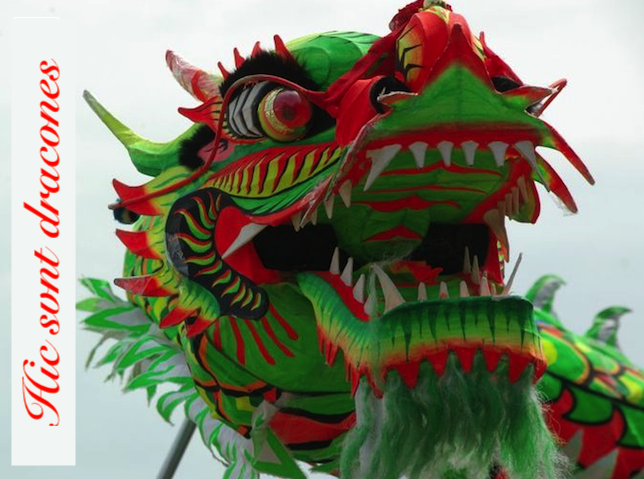
\includegraphics[width=0.75\textwidth]{imagenes/hic-svnt-dracones}
	\vspace{3cm}
\end{titlepage}

\tableofcontents




La confección de este texto es fruto de una larga experiencia como profesor de matemáticas de secundaria y para ello me he basado en mis más de treinta años de docencia  y en la de tantos autores que han contribuido a la explicación de estos conceptos a multitud de alumnos. En especial me he basado en los apuntes de `Cálculo diferencial e integral de funciones de una variable', del profesor Francisco Javier Pérez González, del Departamento de Análisis Matemático de la Universidad de Granada y apuntes del profesor J.A. Gálvez, del departamento de geometría y topología también de la universidad de Granada (ambos apuntes los encontré en la red), así como textos célebres como el Thomson, Apostol, Spivak y otros. También apuntes y problemas de libros de texto de segundo de bachillerato como el que usamos en mi IES los últimos años Anaya, asímismo he acudido a  los de la `Marea Verde', SM, `Curso práctico de matemáticas de COU' de ed. Edunsa y otros;  así como los apuntes y problemas encontrados en la web y, en ocasiones, de la inestimable Wikipedia.También he usado exámenes de EBAU de varias comunidades autónomas. Gracias a todos ellos por su inestimable ayuda para la confección de este pequeño texto que espero que sirva a alguien y que escribo libre de todo tipo de derechos.

Los apartados, teoremas y los ejercicios de mayor nivel estarán marcados con el símbolo $\divideontimes$. Exceden los contenidos de un curso de segundo de bachillerato pero son altamente recomendables para el alumnado que necesite ampliar sus conocimientos matemáticos en cursos posteriores.

\section{Cómo estudiar matemáticas}

 
Las Matemáticas son una asignatura que no deja indiferente a ningún estudiante. Algunos la aman y otros la odian; siendo este segundo grupo mucho más numeroso que el primero en la mayoría de las ocasiones. Sin embargo, muchos de los estudiantes que odian las matemáticas lo hacen porque no saben cómo estudiarlas para obtener buenos resultados.

Las Matemáticas son una de esas asignaturas en las que las horas de estudio no tienen una relación directa con la nota. Por mucho que hayas estudiado, si no eres capaz de solucionar el problema del examen, estás perdido. No obstante, existen algunas técnicas para aprender matemáticas que pueden hacer que, independientemente de tu nivel, le saques más partido a tu tiempo de estudio y aumentes tus probabilidades de éxito. ¡Hasta es posible que te acabes uniendo al grupo de amantes de las matemáticas!

\emph{Cómo Estudiar Matemáticas:}
 
\begin{enumerate}
	 

\item Práctica, Práctica y Más Práctica

Es imposible aprender matemáticas leyendo y escuchando. Para aprender matemáticas hay que ponerse el mono de trabajo y lanzarse a hacer ejercicios matemáticos. Cuanto más practiques, mejor. Cada ejercicio tiene sus particularidades y es importante haber realizado el máximo número de ejercicios posibles antes de enfrentarnos al examen. Este punto es el más importante de todos y la base del resto de técnicas para estudiar matemáticas de esta lista.

Una vez que entendiste los ejemplos explicados en clase, desarrolla ejercicios o problemas con solución para complementar tus conocimientos. Trata de hacerlos sin ver la respuesta y luego, si ni lo puedes terminar, ayúdate de la solución y sigue desarrollando, siempre preguntándote ?`por qué se realiza dicho paso? Se trata de que poco a poco no tengas necesidad de utilizar las soluciones y llegará el momento, después de unos pocos ejercicios, en que ya no necesites de ellas para desarrollar y entender completamente los problemas

No pienses que escuchando la explicación de muchos ejercicios y problemas, donde un profesor te explica y entiendes un 100$\%$, es lo más importante para aprender Matemáticas. La clave del éxito es \emph{¡PRACTICAR!}

\item Revisa los Errores

Cuando estés practicando con ejercicios, es muy importante que compruebes los resultados y, más importante aún, que te detengas en la parte que has fallado y examines el proceso en detalle hasta asimilarlo. De nada sirve comparar resultados si no sabes en qué te has equivocado. Por eso es conveniente que tengas unos buenos apuntes con problemas resueltos. De esta manera, evitarás cometer los mismos fallos en el futuro. También es recomendable apuntar todos tus fallos y repasarlos repetidamente antes del examen.

Toma buenos apuntes: Sé ordenado, utiliza un solo cuaderno para el curso y escribe claramente usando, en lo posible, tus propias palabras para que puedas entender cuando estudies. Copia todo lo que el profesor diga y escriba en la pizarra, anotando los porqués de cada paso, ya que uno siempre puede olvidar lo escuchado y cuando vuelvas a leer tus apuntes podrás recordarlos rápidamente.

Observa y apunta si el profesor hace hincapié en ciertos puntos basándose en repeticiones, ejemplos, diagramas, comentarios extensos, etc., éstos son casi siempre parte importante de los temas.

\item Domina los Conceptos Clave

¡No intentes aprenderte los problemas de memoria! Los problemas matemáticos pueden tener miles de variantes y particularidades, por lo que es inútil aprendernos problemas de memoria sin entenderlos. Es cambio, es mucho más efectivo dominar los conceptos importantes y el proceso de resolución de los problemas.

Recuerda que las Matemáticas son una asignatura secuencial, por lo que es importante asentar una base firme dominando los conceptos clave y teniendo claras las fórmulas matemáticas esenciales.

\item Consulta tus Dudas

Puede que en muchas ocasiones te sientas atascado en una parte de un problema o que simplemente no entiendas el proceso. Lo común en estos casos es simplemente pasar de ese problema y pasar al siguiente. Sin embargo, es recomendable despejar todas las dudas que tengas en la resolución de un problema.

Por tanto, puede ser buena idea estudiar junto a algún/a compañero/a con el que consultar dudas y trabajar juntos en problemas más complejos. O, mejor todavía, ¿por qué no te unes a un grupo de estudio en el que puedes plantear tus dudas y trabajar colaborativamente? Asimismo, recuerda plantearle al profesor/a las dudas que tengas, ya sea en clase o en una tutoría.

\item Crea un Ambiente de Estudio sin Distracciones.

Las Matemáticas son una asignatura que requiere más concentración que ninguna otra. Un ambiente de estudio adecuado y libre de distracciones puede ser el factor determinante para conseguir resolver ecuaciones o problemas de geometría, álgebra, trigonometría o complejos. Si te gusta estudiar con música, puede ser una buena idea escucharla de fondo para relajarte y favorecer un ambiente de máxima concentración; la música instrumental es la más recomendable en estas ocasiones.

¡Ah, y no olvides que es importante también tener confianza en uno mismo y afrontar el examen sabiendo que te has preparado adecuadamente!

\end{enumerate}

\emph{Empieza a Estudiar Matemáticas Ahora. ¡Es gratis!}

\section{Guía de lectura}	

En el apéndice \ref{Kit} tenéis lo que debéis recordar, indispensablemente, para abordar con comodidad el curso de segundo de bachillerato. Aseguraos de que conocéis y recordáis todas estas formulas que aparecen en el `Kit de supervivencia para Matemáticas-2'.

\subsection{Preliminares}

El tema empieza con una breve introducción histórica a los problemas que dieron lugar al cálculo infinitesimal.

Se comenta la terminología que se va a utilizar: axiomas, teoremas, condiciones necesarias y suficientes, ...

Puesto que el cálculo se basa, entre otros conceptos, en el cuerpo de los números reales, se exponen una serie de propiedades de los mismos. Lo más importante del tema será tener muy claro todo lo relativo a las desigualdades y valor absoluto. Para ello se dispone de muchos ejercicios resueltos y propuestos al final del capítulo.

Acabamos con la importancia de las demostraciones en matemáticas con ejemplos del principio de inducción, la reducción al absurdo y el principio del palomar.

\subsection{Funciones}

Empezamos el tema con el concepto de función real de variable real, dominio, recorrido y gráfica.

Pasamos a estudiar las operaciones básicas con funciones así como la composición y la existencia de función inversa en casos de inyectividad.

Seguidamente se estudian las transformaciones básicas de funciones y se habla de las funciones definidas a trozos.

Acaba el tema con una colección de ejercicios (resueltos y propuestos, con solución) para afianzar los conceptos estudiados.

\subsection{Límites y Continuidad}

Después de introducir el concepto de continuidad con un ejemplo de la física pasamos a un estudio intuitivo de los límites así como una colección de ejercicios para repasar el cálculo de límites.  Posteriormente damos las definiciones formales de estos importantes conceptos.

Continuamos el tema con el estudio de la continuidad de las funciones y con otra colección de ejercicios sobre este concepto.

El tema acaba con los importantes teoremas sobre funciones continuas en intervalos cerrados: Bolzano, Darboux y Weiertrass. A estos teoremas también les acompañan una batería de ejercicios resueltos y propuestos.

\subsection{La Derivada}

En el tema se repasan el concepto de derivada y las reglas de derivación de las funciones elementales, así como la regla de la cadena. Todo ello se supone conocido de cursos anteriores.

Se incide en la relación entre continuidad y derivabilidad y se introducen nuevas técnicas de derivación: la derivación implícita, logarítmica y de la función inversa. Se aprende a derivar funciones a trozos y se introducen las derivadas enésimas. Acabamos el tema con el importante concepto de `diferencial' como primera aproximación (lineal) de una función.

Como siempre, acompañamos el tema con una buena colección de ejercicios resueltos paso a paso así como una colección de ejercicios propuestos con su solución.

\subsection{Aplicaciones de la derivada}

Rectas tangente y Normal a una función en un punto.

Información de la primera derivada (crecimiento y extremos, extremos absolutos, `optimización de funciones').

Información de la segunda derivada (curvatura e inflexiones). 

Problemas de encontar parámetros dadas determinadas condiciones de la función.

Teoremas relativos a funciones derivables.:  los teoremas vistos, el th. de Roll (con sus tres hipótesis) asegura cuando una función tiene un extremo en un intervalo. El Teorema del Valor Medio (con sus dos hipótesis) asegura que se puede, al menos en un punto, trazar la tangente paralela a la cuerda que une los extremos de la función. Importantísima la regla de L'Hôpital, se aplica límites de cocientes con indeterminación $0/0$ ó $\infty / \infty$.

Acabamos el tema con la representación gráfica de funciones explícitas.

Aparte de incluir ejemplos de muchos casos, también hemos introducido problemas resueltos y propuestos con solución de cada uno de los apartados anteriores.

Acabamos el tema, como siempre, con una colección de problemas resueltos y propuestos del tema.

\subsection{Desarrollos de Taylor y MacLaurin}

El tema, como el símbolo $\divideontimes$ indica, excede de los objetivos de un curso de segundo de bachillerato, pero se ha intentado presentar de forma sencilla para que sirva como introducción a aquellos/as alumnos/as que deseen ampliar sus conocimientos matemáticos de cara a afrontar, más preparados, la nueva carrera elegida. 

Unas sencillas consideraciones sobre espacios vectoriales nos permiten introducir la fórmula de Taylor para funciones polinómicas. Hemos hecho una generalización para aproximar, bajo determinadas condiciones, una función $f(x)$ por un polinomio de Taylor de orden $n, \; P_n(x)$ y, a la vez, dar una cota del error cometido al hacer tal aproximación a través del resto de Lagrange.

Se ven los desarrollos de MacLaurin y Taylor para alguna funciones conocidas y se muestran unos ejemplos de su potenciabilidad para cálculo de valores en funciones complicadas sin más que calcular el valor numérico de un polinomio.

Entre las aplicaciones que hemos visto, con ejemplos incluidos, de estos desarrollos están las Condición Necesaria y Suficiente  para que un punto sea Extremo Relativo o Punto de Inflexión. También hemos visto la aplicación de los desarrollos de Taylor y MacLaurin al cálculo de límites.

Debido a la dificultad del tema, solo contiene ejemplos y algún ejercicio resuelto, pero no ejercicios propuestos.

\subsection{La integral indefinida}

Prestad mucha atención a este tema, es importantísimo para alumnos/as que deseen cursar estudios superiores que necesiten de una ampliación matemática fuerte. \emph{`A la facultad se debe llegar sabiendo integrar'}.

En el tema se define el concepto de primitiva o anti-derivada de una función y su generalización a la integral indefinida, así como sus propiedades (linealidad de la integral indefinida).

Se encuentran las integrales de las funciones elementales y se extienden a las funciones compuestas (regla de la cadena), lo que da lugar a la `tabla de integrales inmediatas', que aparecerá más desarrollada en el apéndice \ref{app:tabla-integrales}.

A continuación se estudian algunos métodos de integración: integración por partes, integración de funciones racionales e integración por cambio de variable o sustitución, apartado en el que se ven algunos casos sencillos.

Se da, como ampliación, el `método de Hermite' de integración de funciones racionales con raíces complejas múltiples en el denominador.  

Se estudian, con ejemplos y ejercicios resueltos,  el cálculo de primitivas bajo determinadas condiciones.

Aunque el tema, como todos los demás, está repleto de ejemplos, ejercicios resueltos y ejercicios propuestos con solución para cada apartado, al final se ofrece una colección de unos 100 ejercicios propuestos con solución para practicar. Recordad: \emph{`A la facultad se debe llegar sabiendo integrar'}.

Acabamos el tema con un apartado de `curiosidades'.

\subsection{La integral definida}

Empezamos el tema con una introducción histórica al a la integral definida como la solución al problema de encontrar el área bajo una curva. Definimos qué se entiende por trapecios mixtilíneos, particiones del intervalo de integración y dos aproximaciones, una por exceso ($U$) y otra por defecto ($L$) de las sumas de Riemann. Haciendo un paso al límite y teniendo en cuenta el teorema del  criterio del Sandwich en el cálculo de límites que se ve en el tema 3, se define la integral definida como `suma de infinitas cantidades infinitesimales'.

Pasamos a ver que cualquier función continua en un intervalo $]a,b[$, o que tenga un número finito de discontinuidades evitables o de salto finito en el intervalo de integración es integrable. Seguidamente, con la idea en mente de que la ID (Integral Definida) representa el área encerrada por $f$ (si $f>0$), exponemos las `propiedades de la ID', para acabar viendo el `teorema de la media para el calculo integral', que permite calcular el valor medio de una función ctna. en un intervalo $<f>$.

En la segunda sección es donde relacionamos este nuevo concepto de ID -- integral definida--  (cálculo de áreas bajo curvas) con la noción de Derivada (cálculo de la pendiente de la recta tangente a una función en un punto). Definiendo una nueva función llamada `función área' y derivándola encontramos la sorprendente relación entre ambos conceptos: `Teorema Fundamental del Cálculo Integral y Regla de Barrow'. Unos corolarios a estos teoremas nos permiten derivar integrales.

Estudiamos el caso del cambio de variable en ID, que exige que éste sea inyectivo y permite extender el cambio elegido a los límites de integración.

Hablamos también de lo que llamaremos integrales impropias: cuando alguno (o ambos) de los límites de integración son $\infty$ y cuando $f$ presenta discontinuidades asintóticas (de salto infinito) en el intervalo de integración.

Terminamos esta sección con unos cuantos ejemplos de todo lo visto en ella.

En la tercera sección, aplicaciones de la ID, vemos las aplicaciones al cálculo de límites, \emph{el cálculo de áreas de figuras planas} (este es el más importante en segundo de bachillerato), el cálculo de longitudes de arcos de curvas, el cálculo de volúmenes de los cuerpos de revolución y de sus áreas.

De todo ellos vemos muchos ejemplos así como ejercicios resueltos y propuestos (con solución).

Acabamos (casi) el tema con una vasta colección de ejercicios resueltos y propuestos (con solución).

Para finalizar (ahora sí), presentamos una sección de `Curiosidades y Aplicaciones de la ID'.

\subsection{Introducción a las ecuaciones diferenciales}

El estudio de ecuaciones diferenciales (ecuaciones que involucran a la variable independiente $x$, a una función de ella $y=f(x)$ y a sus derivadas $y', \; y'', ; \cdots$)  es un campo extenso en matemáticas puras y aplicadas, en física y en la ingeniería. Todas estas disciplinas se interesan en las propiedades de ecuaciones diferenciales de varios tipos.

Sin embargo, el contenido de este tema excede al nivel de bachillerato.  Es copia `casi' textual de los apuntes del catedrático J.A. Gálvez, del departamento de Geometría y Topología de la Universidad de Granada, que encontré en internet y al cual agradezco desde aquí su trabajo docente expuesto al público en general.

Si el lector/a lo considera demasiado complicado, puede saltar al siguiente capítulo, pero su importancia es crucial en física e ingenierías.

\subsection{Introducción al cálculo vectorial en $\mathbb R^3$}

En este tema se introducen los campos escalares y vectoriales, así como los conceptos de derivadas parciales, gradiente, operador nabla, derivada direccional, divergencia, rotacional, laplaciana y operador laplacina. Si al lector le resulta muy tediosso, puede pasarlo por alto, pero su importancia es crucial en física e ingenierías.

\subsection{Apéndices}
\begin{enumerate}[A) ]
\item Kit de supervivencia para matemáticas-ii
	\begin{itemize}
	\item Aritmética y Álgebra
	\item Complejos
	\item Trigonometría
	\item Geometría analítica y vectores 2D	
	\item Análisis
	\end{itemize}
\item Gráficas de las funciones elementales más conocidas
\item Tabla de derivadas
\item Desarrollos es serie de MacLaurin más usuales
\item Tabla de integrales. 
\end{enumerate}


\begin{figure}[H]
	\centering
	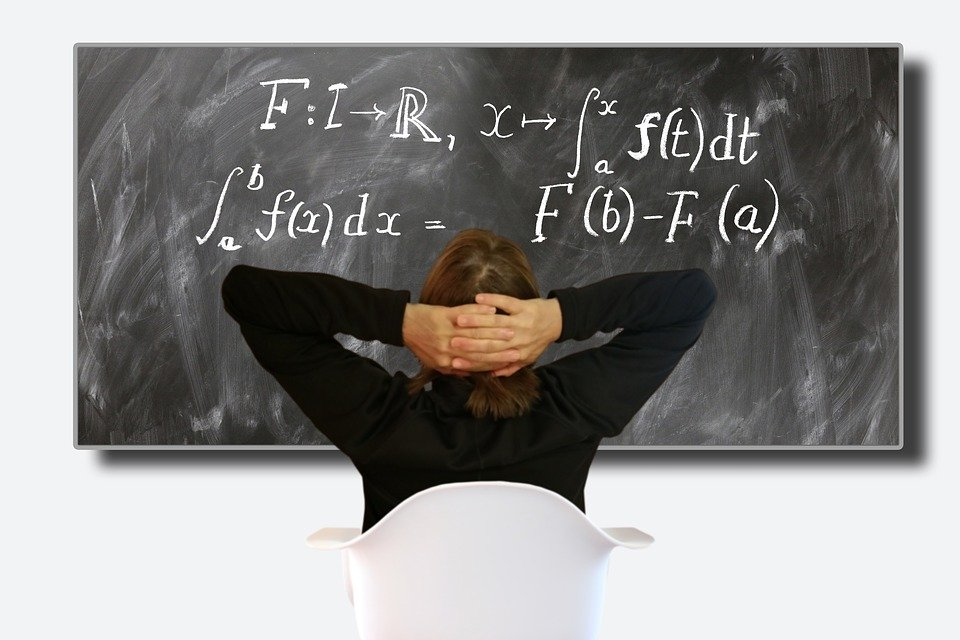
\includegraphics[width=1\textwidth]{imagenes/imagenes00/xiste00.png}
\end{figure}


	\textit{Este material es un conjunto de apuntes personales, que comparto gratuitamente en la red, basados en mi experiencia como profesor, varios textos citados anteriormente y webs de internet. Si hay algún contenido que no he incluido correctamente, hacédmelo saber por e-mail y lo editaré como se pida.  También se agradecería la comunicación de la detección de cualquier error.}

\vspace{10mm}
\emph{Este documento se comparte bajo licencia `Attribution-NonCommercial 4.0 International (CC BY-NC 4.0)'}

\vspace{10mm}

\begin{multicols}{2}
\begin{figure}[H]
	\centering
	
\includegraphics[width=.4
	\textwidth]{imagenes/imagenes00/licencia.png}
\end{figure}
\begin{figure}[H]
	\centering
	
\includegraphics[width=.3
	\textwidth]{imagenes/firma.png}
\end{figure}
\end{multicols}



\part{CÁLCULO DIFERENCIAL}
\chapter{Preliminares.}	\label{preliminares}

	\section{Introducción histórica}
	
		El cálculo infinitesimal es la \emph{matemática del cambio}, tiene dos ramas principales: el cálculo diferencial y el cálculo integral. Ambos forman un poderoso instrumento para atacar múltiples problemas de la física, ingenieras y otras ciencias, incluidas las ciencias sociales.
	
		En sus inicios, s. XVII, el cálculo surgió al buscar la solución a dos problemas fundamentales inspirados por la física: el problema del trazado de rectas tangentes a una función en un punto, que permitirá la posibilidad de encontrar valores óptimos (máximos o mínimos) para estas funciones y que dará como resultado el cálculo diferencial y, el segundo problema, determinar la longitud de una curva, el área que hay bajo la misma y el cálculo de volúmenes, que dará lugar al cálculo integral. Quizás el descubrimiento más importante es que hay una conexión inesperada entre dos problemas clásicos aparentemente no relacionados: encontrar tangentes a una curva y calcular áreas. Lo veremos en el capítulo de la Integral Definida y le llamaremos \textit{Teorema Fundamental del Cálculo Integral }.
	
		Derivadas e integrales resolvían problemas que habían puesto a prueba el ingenio de matemáticos anteriores. Velocidades, tangentes, máximos y mónimos podan encontrarse utilizando diferenciación. Longitudes, áreas y volúmenes podan calcularse por integración. Parecía que las pautas de la naturaleza estaban escritas en el lenguaje del cálculo infinitesimal. 
	
		Fue ya en el s. XIX, con la construcción del cuerpo de los números reales, del concepto de función real y del concepto de límite, cuando se establecieron de manera rigurosa los fundamentos del cálculo. 

		%\vspace{5mm}
	
		\begin{figure}[H]
			\centering
			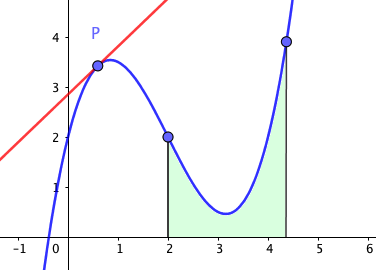
\includegraphics[width=0.5\textwidth]{imagenes/imagenes01/T01IM01.png}
			\caption{Los dos problemas clásicos del cálculo: trazado de tangentes y áreas bajo curvas.}
		\end{figure}
		
		Hemos visto como surgió el cálculo. Pero ?`\emph{qué es realmente el cálculo infinitesimal}?: El cálculo suele dividirse en dos partes, denominadas cálculo diferencial y cálculo integral. El cálculo diferencial investiga las propiedades de las razones de cambio de variables que están vinculadas por medio de ecuaciones. Por ejemplo, un resultado fundamental del cálculo diferencial es que si $y = x^n$, entonces la razón de cambio de $y$ con respecto a $x$ es $n x^{n-1}$. Resulta que cuando se usa la intuición para pensar en ciertos fenómenos (movimiento de los cuerpos, cambios en la temperatura, crecimiento de poblaciones y muchos otros), se llega a postular ciertas relaciones entre estas variables y sus razones de cambio. Estas relaciones se escriben en una forma conocida como ecuaciones diferenciales. Así, el objetivo principal de estudiar cálculo diferencial consiste en comprender qué son las razones de cambio y cómo escribir ecuaciones diferenciales. El cálculo integral proporciona métodos para recuperar las variables originales conociendo sus razones de cambio. La técnica para hacer esto se denomina integración, y el objetivo fundamental del estudio del cálculo integral es aprender a resolver las ecuaciones diferenciales proporcionadas por el cálculo diferencial.
	
	
	
	\section{ Axiomas, definiciones, teoremas $\; \divideontimes$}
	
	Para entender bien este apartado, el/la lector/a interesaso/a puede consultar el apéndice \ref{ap:logica} de `Intoducción a la lógica'. 
	
Suele decirse que en matemáticas no hay nada más que	axiomas y teoremas (bueno, también hay conjeturas, proposiciones, definiciones,...). Todo lo que se demuestra es un teorema, por ello el nombre teorema se reserva para resultados que se consideran realmente importantes y que ha costado esfuerzo llegar a probarlos. Se usan también los términos: corolario, lema, proposición, definición y otros. Pero la estructura de una teoría matemática  se resume en un conjunto de axiomas y de teoremas que se deducen de ellos mediante reglas de inferencia lógica. Veamos que es cada una de estas estructuras lógicas de las matemáticas.
	
		AXIOMA: enunciado cuya veracidad es admitida por todos/as y no necesita demostración.
	
		DEFINICIÓN: los objetos matemáticos existen mediante definiciones. Por ejemplo, un número puede ser natural y se llama número compuesto o número primo, par o impar, siempre que cumpla condiciones precisas y específicas. Estas condiciones son la definición del concepto.
	
		PROPOSICIÓN: enunciado cuya veracidad se ha demostrado.
	
		LEMA: proposición que es preciso demostrar antes de demostrar un teorema para que la demostración de este último no sea excesivamente larga.
	
		TEOREMA: enunciado en el que, a partir de una suposiciones iniciales (HIPÓTESIS) se consigue demostrar otro enunciado (TESIS).
	
		COROLARIO: son teoremas consecuencia inmediata de otro teorema anterior al que se le considera de mayor importancia.
		
		 Un teorema escrito en la forma H (hipótesis)$\; \to\; $ T (Tesis), se llama \emph{teorema directo} y se lee "si se verifica H, entonces se verificará T". Hay otros teoremas relacionados con el directo:
		
		\emph{Teorema contrario:} no H $\; \to\; $ no T
		
		\emph{Teorema recíproco:} T $\; \to\; $ H
		
		\emph{Teorema contrarrecíproco:} no T $\; \to\; $ no H
		
		Ejemplos:
		
		\hspace{10mm} Directo: Ser madrileño (H) implica ser español (T)
		
		\hspace{10mm} Recíproco: Ser español (T) implica ser madrileño (H): No se verifica, ser español no implica ser madrileño.
		
		\hspace{10mm} Contrario: no ser madrileño (no H) implica no ser español (no T): No se verifica, se puede ser español sin ser madrileño, p.e., siendo andaluz.
		
		\hspace{10mm} Contrarrecíproco: no ser español (no T) implica no ser madrileño (no H): Sí se verifica, si no eres español no puedes ser madrileño.
			
		\vspace{4mm} CONDICIONES NECESARIAS Y SUFICIENTES: 
		
		$M \to A \quad$: A es \emph{condición necesaria} para que se cumpla M. Ejemplo: M="ganar la liga de fútbol de primera división", A="jugar en primera división"	
		
		$B \to M \quad$: B es \emph{condición suficiente} para que se cumpla M. Ejemplo: M="ganar la liga de fútbol de primera división", B="ser el equipo con más puntos al finalizar la liga".
		
		$C \longleftrightarrow  M \quad$:  C es \emph{condición necesaria y suficiente} de M. Ejemplo: M="ganar la liga de fútbol de primera división", C="recibir el trofeo de campeón al finalizar la liga".
		
		
		\vspace{4mm} \emph{Nota:} Cuando acaba la demostración de un teorema es usual advertírselo al lector por si ha de volver a empezar a releer la misma. Para ello se suele escribir cosas como ``c.q.d'', como queramos demostrar; ``q.e.d'', quod erat demonstrandum (en latín) y, la que usaremos nosotros, que será el símbolo $\Box$ situado al final y a la derecha de la última línea de la demostración.
		
		

	\section{Los números reales}
	
	El hombre ha necesitado, a través de su historia, de los números naturales para contar, de los enteros para el comercio, de los racionales para sus construcciones. Ya los griegos (escuela pitagórica) se dieron cuenta de que existían otro tipo de números extraños a los que llamaron irracionales, lo que nos lleva a nuestro objetivo de los números reales, base del cálculo.
	
		Números naturales $\mathbb N$: 1, 2, 3, ...
	
		Números enteros $\mathbb Z$: ... , -2, -1, 0, 1, 2, 3, ...
	
		Números racionales $ \mathbb {Q} =\left\{\dfrac p q; \  p,q\in \mathbb {Z}; \ q>0; \ mcd\ (p,q)=1 \right\}$. Es decir, son el conjunto de las fracciones irreducibles de números enteros con denominador positivo (no nulo). Sabemos que su expresión decimal siempre es un número entero, decimal exacto o decimal periódico y sabemos pasar de escritura decimal (en estos casos) a escritura en forma de fracción y viceversa. 
		
		Pero hay números cuya expresión decimal es infinita y no periódica, luego no se pueden expresar como fracción ($\sqrt 2$ no es racional, lo veremos más adelante, en el apartado dedicado a la demostración por \emph{reducción al absurdo}) (sección \ref{reduc-absurd}). Este nuevo tipo de números son los IRRACIONALES ($\pi, \ e, \ \sqrt[3]{5}, \ ..$)
	
		Número reales $\mathbb R$: es el conjunto formado por todos los números racionales e irracionales.
	
		Dados $x,y \in \mathbb R$, representaremos por $x+y$ la suma de números reales y por $xy$ el producto.
	
		
	
	\subsection{Axiomas algebraicos}
		
		\begin{axio}[Axiomas Algebraicos] Responden de las propiedades de la suma y producto de números reales. Son los siguientes:	
		\end{axio}
 
	
		\begin{itemize}
		\item ASOCIATIVAS:  
			\begin{equation}
			\forall x,y,z  \in  \mathbb R: \quad
			(x+y)+z=x+(y+z);  \qquad (xy)z=x(yz)
			\end{equation}
	
		\item CONMUTATIVAS:  
			\begin{equation}
			\forall x,y  \in  \mathbb R: \quad
			x+y=y+x;  \qquad xy=yx
			\end{equation}
	
		\item ELEMENTOS NEUTROS:  Hay dos números reales \textit{distintos} $0$ y $1$ tales que $\forall x \in \mathbb R$ se verifica:
			\begin{equation}
		    0+x=x;  \qquad 1x=x
			\end{equation}
	
		\item ELEMENTOS OPUESTO E INVERSO:  Para cada número real $x$ hay un número real llamado \textit{opuesto} de x, que representamos por $-x$ tal que: 
			\begin{equation}
			x+(-x)=0
			\end{equation}
			Para cada número real $x$ distinto de cero, $x \neq 0$, hay un número real llamado \textit{inverso} que representamos por $x^{-1}$, tal que  
			\begin{equation}
			xx^{-1}=1
			\end{equation}
		\item DISTRIBUTIVA:  
			\begin{equation}
			\forall x,y,z  \in  \mathbb R: \quad
			(x+y)z=xz+yz
			\end{equation}
		\end{itemize}
	
		
	
		\begin{prop}
		Se verifican las siguientes igualdades:	
		\begin{equation}
		0x=0; \qquad (-x)y=-xy; \qquad (-x)(-y)=xy
		\end{equation}
		\end{prop}
	
		\begin{proof}
		
	 	Probaremos primero que 0x = 0. Por la propiedad distributiva:$(0 + 0)x = 0 x + 0 x$ . 
	 	
	 	
	 	Como consecuencia del elemento neutro es $0 + 0 = 0$. Obtenemos as que $0x=0x+0x$.
	 	Teniendo en cuenta el elemento neutro de la suma:  $0 x = 0$.
	 	Probaremos ahora que $(-x)y =  - (xy)$. Tenemos que $xy + (-x)y = (x + (-x))y = 0 y = 0$. Donde hemos usado el opuesto, la distributiva y el apartado anterior. 
		
		La igualdad $xy + (-x)y = 0$ nos dice, por el elemento opuesto, que $(-x)y$ es el opuesto de $xy$. Eso es justamente lo que queramos probar

		Finalmente, la igualdad $(-x)(-y) = xy$ es consecuencia inmediata de la anterior.
	
		\end{proof}

		El símbolo $-x$ debe leerse siempre el opuesto de $x$ y no menos $x$. La razón es que la palabra menos  remite a una idea de orden (si hay menos  es porque hay más ) y el significado de $-x$ es puramente algebraico y nada tiene que ver con la idea de orden de la que ni siquiera hemos hablado  !`No cometas el error de pensar que $-x$ es negativo!

		Notación. Suele escribirse $x - y$ en vez de $x + (-y)$. También, supuesto $y \neq 0$, se escribe $x/y$ o $\frac x y$ en vez de $xy^{-1}$.
	
		
	
	\subsection{Axiomas de orden}
		
		\begin{axio}[Axiomas de orden]
			La ordenación de números reales establece que su representación en una recta consiste en fijar un punto, \textit{origen}, donde se coloca el $0$ y los números situados a su derecha son los \textit{positivos}, representados por $\mathbb R^+$. Las propiedades del orden son:
		\end{axio}
		
		\begin{itemize}
		\item LEY DE TRICOTOMÍA. Para cada número real $x$ se verifica una sola de las tres siguientes afirmaciones:  $x=0$, $x$ es positivo, $-x$ es positivo.
		\item ESTABILIDAD DE $\mathbb R^+$. La suma y producto de números positivos también es un número positivo.
		\item RELACIÓN DE ORDEN. La ley de Tricotomía en particular dice que el $0$ no es positivo. Por otra parte, como $x+(-x)=0$, por la ley de estabilidad de $\mathbb R^+$ concluimos que $-x$ no es positivo. Los elementos del conjunto $\mathbb R^- = \{ -x: x\in \mathbb R^+ \} $ se llaman \textit{números negativos} y son los opuestos a los números positivos.
		\end{itemize}
	
		
		
		\begin{defi} Para $\;x,y  \in \mathbb R\;$, escribimos $\;x<y\;$ o $\; y>x\; $ para indicar que $\; y-x \in \mathbb R^+\; $ y escribimos $\; x\le y$ o $y \ge x\; $ para indicar $\; y-x \in \mathbb R^+ \cup \{ 0 \} = \mathbb R^+_0\; $(Notación: $\; \mathbb R^-_0=\mathbb R^-\cup \{ 0 \};\; \mathbb R^*=\mathbb R \sim \{ 0 \}\; $)
		\end{defi}
		
	
		\begin{prop}
		Para todo $x\neq 0$ se verifica que $x^2>0$. En particular, $1>0$.
		\end{prop}
	
		\begin{proof}
		Si $\;x\neq 0 \;$, por la ley de tricotomía o bien $x$ es positivo o bien $-x$ es positivo. Como $\; x^2=xx=(-x)(-x)\; $, concluimos que $x^2$ es positivo, nos apoyamos en la ley de estabilidad del producto en $\mathbb R^+$, ambas leyes de los axiomas de orden de los números reales.. En particular tenemos que $1^2=1>0$. !`El $1$ es positivo! 
		\end{proof}
		
		
	\subsection{Propiedades topológicas de los números reales}
	 
	 Daremos, sin demostración, las siguientes propiedades de los números reales:
	 
	
	\begin{enumerate}[Prop.R.1]
	
		\item $\mathbb R$ es \emph{arquimediano}: $\forall x \in \mathbb R \; \; \exists n \in \mathbb N \; : \; x<n$
		\item $\forall x \in \mathbb R \; \forall y \in \mathbb R^{+} \;  \exists n \in \mathbb N \: : \; x<ny $. Geométricamente significa que todo segmento ($x$), por grande que sea, se puede recubrir con unidades tan pequeñas como se quiera ($y$). De otro modo, con una regla, por pequeña que sea, se puede cubrir cualquier distancia (basta colocarla sucesivamente las veces que haga falta).
		\item $\mathbb R\; $es \emph{denso}: 
		
		$a)\quad \forall x,y \in \mathbb R$ con $x<y,\;\; \exists q \in \mathbb Q:\; \; x<q<y$
		
		$b)\quad \forall x,y \in \mathbb R$ con $x<y,\;\; \exists \alpha  \in \mathbb R \sim \mathbb Q: \; \; x<\alpha<y$
		
		 
	\end{enumerate}
	
	\subsection{Desigualdades}
	 Las desigualdades son un tema muy importante que hay que aprender a manejar correctamente mediante la práctica de muchos ejemplos y ejercicios. Siempre hay que respetar las reglas generales que las gobiernan y se dan en el siguiente teorema.	
			
		\begin{teor}[Reglas para trabajar con desigualdades.] 	
		Sean $x,y,z \in \mathbb R$ 
		\end{teor}
		\begin{enumerate}
			\item $x \le y \;$ e $\; y\le z\; $ implican que $\; x\le z$
			\item $x \le y \;$ e $\; y\le x\; $ implican que $\; x=y$
			\item Se verifica exactamente una de las tres relaciones: $\; x<y\; $, $\; x=y \; $ o $\; y<x$
			\item $x<y\; $ implica que $\; x+z<y+z\; $
			\item $x<y,\; z>0$ implican que $\; xz<yz$
			\item $x<y,\; z<0$ implican que $\; xz>yz$
			\item $xy>0\;$ sí, y solo si, $x$ e $y$ son los dos positivos o los dos negativos. En consecuencia, si $x\neq 0$, entonces $\; x^2>0\; $ y, en particular, $1>0$
			\item $z>0\;$ implica que $\; \frac 1 z >0$
			\item supuestos $x$ e $y$ ambos positivos o ambos negativos, se cumple que $\; x<y \; $ implica $\; \frac 1 y < \frac 1 x \;$
		\end{enumerate}
	
		\begin{proof}
			Todas estas propiedades son fáciles de probar. P.e., el apartado 5, si $x<y$ se tiene que $y-x>0$. Tomando $z>0$, también será $z(y-x)>0$, es decir, $zy-zx>0$, o sea $zx<zy$. Lo único que hay que tener en cuenta para demostrar todos los apartados de este teorema son las definiciones de los símbolos $<$ y $>$ y los axiomas algebraicos y de orden de los números reales. El resto de la demostración se deja como ejercicio.
		\end{proof}
		
		
	\subsection{Ínfimo y Supremo. Axioma de completitud $ \; \divideontimes$}
	
	Antes de enunciar el último axioma de los números reales, veamos las siguientes definiciones:
	
		\begin{defi} Sea $A \subset \mathbb R$, entonces
		
			\begin{itemize}
				\item [*] Si existe $x \in \mathbb R$ tal que $x>a$ para todo $a \in A$, entonces $x$ se llama 'cota superior' de A y se dice que el conjunto $A$ está 'acotado superiormente'.
				\item [*] Si existe $x \in \mathbb R$ tal que $x<a$ para todo $a \in A$, entonces $x$ se llama 'cota inferior' de A y se dice que el conjunto $A$ está 'acotado inferiormente'.
			\end{itemize}
		
		\end{defi}
		
		\begin{defi}
		Sea $A \subseteq  \mathbb R$ acotado superiormente y supongamos que existe un $a\in \mathbb R$ que satisface las siguientes dos condiciones:
		
			\begin{itemize}
				\item [---] $a$ es una cota superior de $A$
				\item [---] si $b\in \mathbb R$ es cota superior de $A$, entonces $a\le b$
			\end{itemize}
			
		Entonces $a$ es el 'supremo' de A, es 'la menor de las cotas superiores"
		\end{defi}

		\begin{defi}
		Sea $A \subseteq \mathbb R$ acotado inferiormente y supongamos que existe un $a\in \mathbb R$ que satisface las siguientes dos condiciones:
		
			\begin{itemize}
				\item [---] $a$ es una cota inferior de $A$
				\item [---] si $c\in \mathbb R$ es cota inferior de $A$, entonces $a\ge c$
			\end{itemize}
			
		Entonces $a$ es el 'ínfimo' de A, es 'la mayor de las cotas inferiores"
		\end{defi}
		
		\begin{axio}Axioma de completitud.
		
			\begin{itemize}
				\item [---] Todo conjunto no vacío de números reales acotado superiormente tiene supremo-
				\item [---] Todo conjunto no vacío de números reales acotado inferiormente tiene ínfimo.
			\end{itemize}
			
		\end{axio}

	
		\begin{defi} Se dice que un conjunto no vacío de números reales $A \subset \mathbb R$, tiene \emph{máximo} si hay un número $M\in A$ que es el mayor de todos los elementos de A, es decir, $x\le M,\; \forall x \in A$. En este caso escribimos $M=max\, A$. Si $\exists m \in A : m\le x;\, \forall x \in A$, m es el \emph{mínimo} de A, $m=min\, A$.
		
			De otro modo, si el supremo de $A$ está en $A$, se le llama máximo. Si el ínfimo de $A$ está en $A$, se le llama mínimo.
		\end{defi}
		
		
	
	
	\subsection{Valor absoluto}
	
	\begin{defi}[Valor Absoluto.] El valor absoluto de un número real $\, x\in \mathbb R\, $ se define como el número:
	\begin{equation}
		|x|=
		\begin{cases} 
		\;\;  x &\mbox{ si } x\ge 0 \\ 
		\; -x & \mbox{ si } x<0 
		\end{cases}
	\end{equation}	
	\end{defi}
		El valor absoluto es, en matemáticas el \textit{gran positivizador}, $|3|=3;\quad |-2|=2; \quad |0|=0$.
	
	\begin{defi}
	Para cada $\; x\in \mathbb R^+_0\; $, representamos	por $\; \sqrt x\; $ al único número \emph{mayor o igual que cero} cuyo cuadrado es igual a $x$.
	\end{defi}
	En consecuencia, $\; \sqrt {x^2}=|x|\; $ (En efecto, $\;|x|^2=x^2 \; $ y, además, $\;|x| \ge 0 \; $, por tanto: $\; \sqrt {x^2}=|x|\; $)
	
	\begin{teor}[Propiedades del valor absoluto.] 	
	\end{teor}
		\begin{enumerate}
		\item $|-x|=|x|$
		\item $|xy|=|x|\cdot|y|$
		\item $\left| \dfrac x y \right| = \dfrac {|x|}{|y|}$
		\item $|x|\le y\;  \mbox{ es equivalente a } -y\le x \le y $
		\item $|x+y|\le|x|+|y|\qquad$ \emph{\underline{Desigualdad Triangular}}
		\item $\left|\,  {|x|-|y|}\,  \right| \le|x-y|\qquad$ La igualdad se da solo si $xy\ge 0$ 
	\end{enumerate}
	
	\begin{proof}
		Usaremos la estrategia siguiente: a) Para probar que dos números positivos son iguales es suficiente probar que sus cuadrados son iguales; y b) Para probar una desigualdad entre dos números positivos es suficiente con probar esa desigualdad para sus cuadrados.
		Para probar 1, 2, y 3, pe. la 2, tenemos que: 
		
		$|xy|^2=(xy)^2=x^2y^2=|x|^2 |y|^2=\left( |x||y|\right)^2 $
		
		\vspace{2mm}\hspace{-7mm}
		Para la desigualdad triangular:
		
		$|x+y|^2=(x+y)^2=x^2+2xy+y^2=|x|^2+2xy+|y|^2\le $
		$|x|^2+2|xy|+|y|^2= \left( |x|+|y| \right)^2$
		
		\vspace{2mm}\hspace{-7mm}
		La última propiedad: $||x||-|y||^2=x^2-2|x||y|+y^2\le $
		$ x^2 - 2 x y +y^2=(x-y)^2=|x-y|^2 \qquad$ La igualdad se verifica si, y solo si, $xy=|xy|$, es decir, $xy\ge 0$
		\end{proof}
		
		
		
		\begin{proof}[Otra forma de demostar la desigualdad triangular: $|x+y|\le|x|+|y|\;$ ].
		
		
		 Consideraremos 4 casos:
			 i) $x\ge0;\;\;y\ge0;\; \; $
			 ii) $x\ge0;\;\;y\le0;\; \; $
			 iii) $x\le0;\;\;y\ge0;\; \; $
			 iv) $x\le0;\;\;y\le0$	
			
			
			En el caso i) se verifica también que $x+y\ge0\;$ y, obviamente: $|x+y|=x+y=|x|+|y|$. En este caso se verifica la igualdad.
			
			En el caso iv), tenemos que $x+y\le 0$ y nuevamente se verifica la igualdad: $|x+y|=-(x+y)=-x+(-y)=|x|+|y|$
			
			 En el caso ii), cuando $x\ge 0\; $ y $\; y\le0$ , debemos probar que $|x+y|\le x - y$. este caso lo subdividiremos en dos subcasos:
			
			\hspace{10mm}$\diamond$  Si $x+y\ge 0$, tendremos que demostrar que $x+y\le x-y$; es decir, $y\le -y$. lo cual es cierto ya que $y\le 0$ y por tanto $-y\ge 0$
			
			\hspace{10mm}$\diamond$ Si $x+y\le 0$, debemos demostrar que $-x-y\le x-y$, es decir, $-x\le x$, lo cual es cierto ya que $x\ge 0$ y por tanto $-x\le 0$
			
			 Finalmente, el caso iii) puede demostrarse intercambiando $x$ por $y$ en la propiedad anterior. 
		\end{proof}
		
		\begin{proof}[Una tercera demostración de la desigualdad triangular] Haciendo uso se las propiedades del valor absoluto:
		
		$-|x|\le x\le |x|;\quad -|y|\le y\le |y|\quad $ Sumando ambas expresiones:
		
		$-\left( |x|+|y| \right) \le x+y \le \left( |x|+|y| \right)\quad $	Lo cual implica que: $|x+y|\le |x|+|y|$
			
		\end{proof}
		
		 Una figura como demostración sin palabras.
		
		
		\begin{figure}[H]
			\centering
			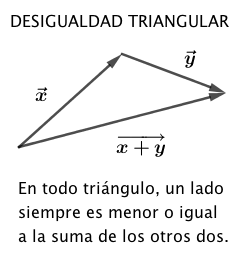
\includegraphics[width=0.4\textwidth]{imagenes/imagenes01/T01IM02.png}
			\caption {Desigualdad triangular: el módulo del vector suma de otros dos siempre es menor o igual a la suma de los módulos de los vectores sumados.}
		\end{figure}
		
		 \begin{defi} Llamamos \emph{distancia} entre dos números $x,y:\quad$ $\forall x,y \in \mathbb R:\; \; d(x,y)=|y-x|$
		\end{defi}
		
		 Se cumplen las siguientes propiedades para las distancias. La demostración se deja como ejercicio, se trata de aplicar las propiedades del valor absoluto.
		
		\begin{enumerate}[PD.1]
			\item  $\forall x \in \mathbb R:\; d(x,x)=0 $
			\item  $\forall x, y \in \mathbb R:\; d(x,y)=d(y,x)$
			\item  $\forall x, y, z \in \mathbb R:\; d(x,z) \le d(x,y)+d(y,z)$
		\end{enumerate}
		
		


		
	
	\subsection{Intervalos}
	
	\begin{defi} Es subconjunto de $I \subset \mathbb R$ tal que $\forall u,w \in I\; $, con $u\neq w\; $, y $\forall v \in \mathbb R\; $ con $u<v<w\; $ se cumpla que $v\in I$. Los intervalos pueden ser abiertos, cerrados y semiabiertos.\end{defi}
	
		\begin{figure}[H]
			\centering
			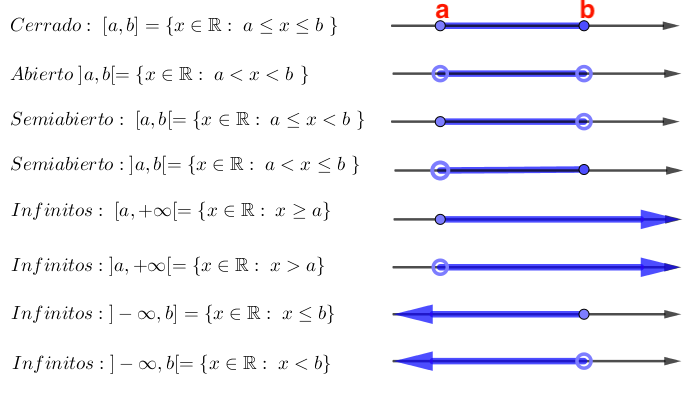
\includegraphics[width=0.7\textwidth]{imagenes/imagenes01/T01IM03.png}
		\end{figure}
		
		
		\begin{defi}[Entorno]: $\forall a \in \mathbb R, \; \forall r \in \mathbb R^{+}: $
		
		Se define el \emph{entorno} de centro $a$ y radio $r$ como todos los números reales cuya distancia a $a$ sea menor que $r$:
		
		$\quad E_r(a)=\{ \forall x \in \mathbb R \;  / \; d(a,x)<r \}=]a-r,a+r[$
		
		Se define el \emph{entorno reducido} de centro $a$ y radio $r$ como todos los números reales cuya distancia a $a$ sea menor que $r$, excluyendo al número $a$:
		
		$\quad E^*_r(a)=\{ \forall x \in \mathbb R \;  / \; 0<d(a,x)<r \}=]a-r,a+r[\sim \{a\}$
			
		\end{defi}
		
		\textbf{Valores Absolutos e Intervalos.}
		\begin{multicols}{2}
		\begin{itemize}
			\item $|x|=k \longleftrightarrow x=\pm k$
			\item $|x|<k \longleftrightarrow -k<x<k \longleftrightarrow ]-k,k[$
			\item $|x|\le k \longleftrightarrow -k\le x\le k \longleftrightarrow [-k,k]$
			\item $|x|> k \longleftrightarrow x>k\quad o \quad x<-k$
			\item $|x|\ge  k \longleftrightarrow x\ge k\quad o \quad x\le -k$
		\end{itemize}
		\begin{figure}[H]
			\centering
			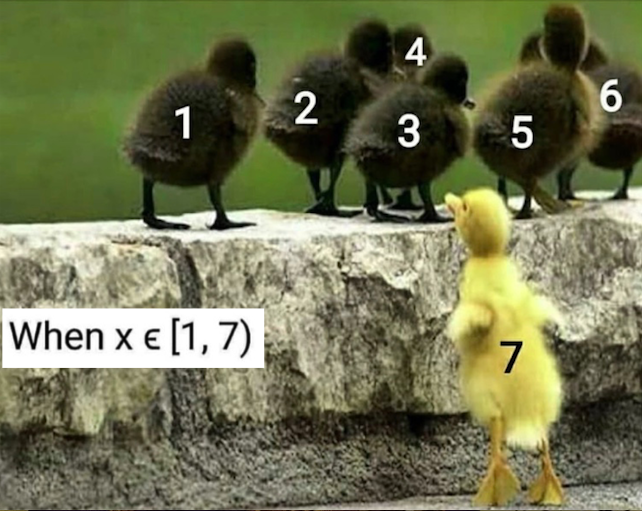
\includegraphics[width=0.4\textwidth]{imagenes/imagenes01/xiste01.png}
		\end{figure}
		\end{multicols}
		
		Recordando lo visto en la sección de supremo e ínfimo, en el intervalo $[2,5[, 2$ es el mínimo y $5$ el supremo.Además, como $2 \in [2,5[$, el intervalo tiene mínimo y éste es igual a $2$. Sin embargo, como $5 \notin [2,5[$ , el intervalo no tiene máximo
		
		\section{ Demostraciones en matemáticas $\; \divideontimes$} \label{demostraciones}
		
		\subsection{Principio de inducción matemática}
		\label{subsec:inducción}
		
		El \emph{Principio de inducción matemática} es un método de demostración que se usa para probar que ciertas propiedades matemáticas se verifican para todo número natural. Por ejemplo:
		$1^2+2^2+3^2+...+n^2=\frac 1 6 n (n+1)(2n+1)$
		
		Podemos comprobar fácilmente que se cumple esta relación para los valores $n$ concretos que se nos ocurra, pero queremos \emph{demostrar} que la relación es válida $\forall n\in \mathbb N$ y para ello usaremos el \emph{Principio de inducción matemática}, que podemos considerar como un axioma y lo entenderemos as:
		
		\begin{axio}[Principio de inducción matemática] Queremos probar que la propiedad $P(n)$ se verifica $\forall n\in \mathbb N$. Tendremos que seguir dos pasos:
			\begin{enumerate}
				\item Comprobaremos que el número 1 cumple la propiedad, es decir, $P(1)$ es cierta.
				\item Comprobaremos que si un número $n$ cumple la propiedad, \emph{entonces} también la satisface el número $n+1$. Es decir, si comprobamos que $P(n)$ es cierta, \emph{entonces} también lo es $P(n+1)$
			\end{enumerate}
			
			"Si tengo una escalera infinita y quiero poder llegar a cualquier peldaño, necesito dos cosas: un primer escalón y saber cómo dar un paso"
		\end{axio}

		
		\begin{ejem} \label{sum-cuad-induc}
		Probar que $\forall n\in \mathbb N$, se cumple:
		$1^2+2^2+3^2+...+n^2=\frac 1 6 n (n+1)(2n+1)$	
		\end{ejem}
		 Evidentemente, para $n=1$ se cumple: $1=1$
		
		\begin{proof}[Apliquemos el método de inducción.]
			
		Supongamos ahora que la propiedad es cierta para $n$, hemos de conseguir demostrar que también lo ha de ser para $n+1$, es decir, se ha de cumplir la propiedad cambiando la $n$ por $n+1$:
		
		$1^2+2^2+3^2+...+n^2+(n+1)^2=\frac 1 6 (n+1) (n+2)(2(n+1)+1)$ (*)
		
		Vamos a por ello, sumemos $(n+1)^2$ a ambos lados de la ecuación que suponemos válida para $n$:
		
		
		$1^2+2^2+3^2+...+n^2\; \; +(n+1)^2=\frac 1 6 n (n+1)(2n+1)\; \; +(n+1)^2=$
		(sacando $n+1$ factor común:)
		$=(n+1) \left( \frac 1 6 n (2n+1) +(n+1) \right)=$
		
		$=(n+1)\frac 1 6 \left(  n (2n+1) + 6(n+1) \right)=$
		$\frac 1 6 (n+1) (2n^2+7n+6)=$
		
		$=\frac 1 6 (n+1) (n+2) (2n+3)\; $ que es la expresión (*) que queramos demostrar.%$\Box$
		\end{proof}
		
		 
		Es necesario subrayar la importancia de la demostración de las dos partes del principio de inducción. Veamos un ejemplo de la importancia de la primera parte:
		
		\begin{ejem}
			Todo número natural es igual al número natural siguiente.
		\end{ejem}
		
		\begin{proof}[Mala aplicación del principio de inducción.]
			
		Aplicando la parte 2 del principio de inducción, resulta que si esto es cierto para $n$, es decir, $n=n+1$, basta con sumar $1$ a cada parte de la igualdad y escribir $n+1=n+1+1=n+2$, también será cierto para $n+1$.
		
		Obviamente la demostración no está acabada y el teorema es falso, pues falta comprobar la primera parte del método de inducción: la propiedad se cumple para $n=1$: falso, $1\neq 2$ %$\qquad \qquad \qquad \qquad \Box$
		\end{proof}
		
		Vamos a ver unos ejemplos a continuación que nos convenzan de la importancia de no quedarse con una conjetura encontrada sino que hay que demostrarla siempre.
		
		\begin{ejem}
			Sea $p(x)=x^4+x+41$, trinomio estudiado ya por Euler. Se tiene que $p(0)=41$, primo; $p(1)=43$, primo, y hasta $x=10$ se obtienen los números 47, 53, 61, 71, 83, 97, 113, 131 y 151 respectivamente, todos primos. Estaríamos tentados a afirmar que en este trinomio, al sustituir $x$ por cualquier número natural se obtiene un número primo, pero no es así, ya que, p.e., para $x=40$ tenemos $p(40)=40^2+40+41=40(40+1)+41=40\cdot 41+41=(40+1)\cdot 41=41^2$, que evidentemente no es un número primo.
		\end{ejem}
		
		 \begin{ejem} Consideremos los números de la forma $N(n)=2^{2^n}+1$. Para $n=0,1,2,3,4$ se obtienen $3, 5, 17, 257, 65537$, que son números primos. Fermat (s.XVII) aceptaba que todos los números obtenidos por esta fórmula eran primos. Fue Euler (s. XVIII) encontró $N(5)=4294967297=641\cdot 6700417$, compuesto.
		\end{ejem}
		
		\begin{ejem}
 			Leibniz (s. XVII) demostró que para cualquier número natural $n$, el número $n^3-n$ es siempre divisible por $3$, el número $n^5-n$ divisible por $5$, $n^7-n$ divisible por $7$. De ahí, supuso que si $k$ era un número natural impar, $n^k-n$ seria divisible por $k$, pero pronto observó que $2^9-2=510$ que no es divisible por $9$.
 		\end{ejem}
 		
 	    \begin{ejem}
 			$F(n)=991n^2+1$ no da nunca un cuadrado perfecto para $n=1,2,3,...$, por muchos das o años que nos dediquemos a ello. En efecto, el primer número natural para el que $F(n)$ resulta un cuadrado perfecto es:
 			
 			$n=12055735790331359447442538767.$
 		\end{ejem}
 		
 		 Con estos ejemplos podemos llegar a una sencilla pero importante conclusión: una conjetura puede ser cierta en muchos casos particulares pero si no hay demostración, nunca será un teorema.
		
		
		\subsection{Reducción al absurdo}
		\label{reduc-absurd}
		
		\begin{axio}[Reducción al absurdo]Una estrategia muy útil para demostrar que algo es cierto es suponer que es falso y llegar a una contradicción, el error habrá sido suponer que lo que queramos demostrar era falso, luego quedara demostrada su veracidad.	
		\end{axio}

		
		\begin{ejem}
			Demostremos que $\sqrt 2$ es irracional.
		\end{ejem}
		\begin{proof}[Apliquemos la demostración por reducción al absurdo.]
			
		Supongamos lo contrario, que $\sqrt 2\in \mathbb Q$, es decir, $\exists a, b\ \in \mathbb Z, \; b\neq 0\; , mcd(a,b)=1$ tales que $\sqrt 2 = \dfrac a b$, irreducible.
		
		Elevando al cuadrado: $2=\dfrac {a^2}{b^2} \to 2b^2=a^2$. Como a la izquierda de la igualdad hay un número par $2b^2$, la parte de la derecha también será par, $a^2$ ha de ser par, pero si el cuadrado de un. número es par es porque ese número también es par, $a$ es par, luego podremos escribir $a=2c$, para algún $c$.
		
		Volviendo ahora a la ecuación $2b^2=a^2$ y sustituyendo: $2b^2=(2c)^2=4c^2 \to b^2=2c^2$ con lo que $b^2$ también será par y lo mismo para $b$, por lo que $b=2d$, para algún $d$.
		
		Hemos conseguido reducir la fracción $\dfrac a b=\dfrac {2c}{2d}=\dfrac c d\; $, pero, por hipótesis $\dfrac a b\; $ era irreducible. Hemos llegado a una \emph{contradicción}, por lo que $\sqrt 2\notin \mathbb Q$
		\end{proof}
		
		
		\subsection{El principio del palomar}
		
		\emph{Si tienes más palomas que palomares, en un palomar debe haber al menos dos palomas.} Esta frase parece una tontera, pero tiene un contenido matemático muy profundo.
		
		\begin{axio}[Principio del palomar]. Si tenemos $n$ objetos sacados de $m$ categorías diferentes, con $n>m$, entonces tendremos al menos dos objetos de la misma categoría.
		\end{axio}
		
		\begin{ejem}
			Hay por lo menos 2 personas en España con el mismo número de pelos en la cabeza.
		\end{ejem}
		\begin{proof}[Aplicación del principio del palomar.]
			
		La cabeza de una persona tiene en torno a 150.000 cabellos y tener un millón de pelos requeriría de una cabeza gigante (nadie tiene un millón de pelos en la cabeza). Asignamos un palomar por cada número de 0 a 1.000.000 y asignamos una paloma a cada persona que irá al palomar correspondiente al número de pelos que tiene en la cabeza. Como en España hay más de un millón de personas, habrá al menos dos personas con el mismo número de pelos en la cabeza.  %$ \qquad \qquad \Box $
		\end{proof}
				
		
		\section{Ejercicios} \label{preliminares-ejercicios}
		
		\subsection{Ejercicios Resueltos}
		
		
		\begin{ejre}
			Supuesto $0<a<x<b$, probar que se cumple: 
			
			$\dfrac 1 x +\dfrac 1 {a+b-x} < \dfrac 1 a + \dfrac 1 b$
		\end{ejre}
		
		\begin{proofw}\renewcommand{\qedsymbol}{$\diamond$}
		
			No parece fácil, a partir del enunciado, llegar a lo que queremos demostrar. Vamos a \emph{trabajar hacia atrás} a ver si conseguimos llegar a la hipótesis. Luego, por elegancia matemática, bastara con reescribir el ejercicio al revés.
			
			Sumemos las expresiones que me dan para que demuestre:
			
			$\dfrac {a+b}{x(a+b-x)}<\dfrac {a+b}{ab}$; como los denominadores son positivos, podemos multiplicar en cruz sin que se altere el sentido de la desigualdad:
			
			 $(a+b)ab<(a+b)x(a+b-x)$. Como $(a+b)>0$, puede pasar dividiendo y cancelarse y queda: $ab<x(a+b-x) \to 0<ax+bx-x^2-ab=(x-a)(b-x)$ Pero como por hipótesis $0<a<x<b$ se tiene que $x-a>0$ y que $b-x>0$, luego, obviamente, $(x-a)(b-x)>0$. Solo queda recorrer ahora el camino hacia atrás.
		\end{proofw}
		
		\begin{ejre}
			Resuelve la ecuación: $|x-1|=3$, y las inecuaciones $|x-1|\le 3\; $ y $\; |x-1|>3$ 
		\end{ejre}
		
		\begin{proofw}\renewcommand{\qedsymbol}{$\diamond$} 
		
			
			* $|x-1| =3 \quad \rightarrow \left\{ 
			\begin{matrix} 
				x-1=3\quad \to \quad x=4 \\ 
				x-1=-3\quad \to \quad x=-2 
				\end{matrix} 
				\right. $
				
		
		 ** $|x-1|\; \le \; 3 \to -3\le x-1 \le 3$, pasando el $-1$ sumando: $-2\le x \le 4$. La solución son todos los números $x\in [-2,4]$ .
		
		 *** $|x-1|>3 \to x-1<-3 \vee x-1>3 \to x<-2 \vee x>4$. La solución es $]-\infty, -2[\; \cup\; ]4, \infty[$	
		\end{proofw}
		
		 \emph{Nota:} Usamos el símbolo $\vee$ como disyunción lógica \emph{o} ($\wedge$ es la conjunción lógica \emph{y}).
		
		\begin{ejre}
			Resuelve: $|2x+4|\ge 6$
		\end{ejre}
		
		\begin{proofw}\renewcommand{\qedsymbol}{$\diamond$}
		
			$|2x+4|\ge 6 \to 2x+4<-6 \; \vee \; 2x+4>6 \to 2x<-10\; \vee \; 2x>2 \to x<-5 \; \vee \; x>1$. Solución: $]-\infty, -5[\; \cup\; ]1, \infty[$
		\end{proofw}
		
		\begin{ejre}
			Resuelve: $|x^2+3|=5;\qquad |x^2+3|<5; \qquad |x^2+3|\ge 5$
		\end{ejre}
		
		\begin{proofw}\renewcommand{\qedsymbol}{$\diamond$}
		
			* $-5=x^2+3=5 \to 
			\left\{ 
			\begin{matrix} 
				x^2+3=-5\quad \to \quad x^2=-8 \to \quad \nexists x\\ 
				x^2+3=5\quad \to \quad x^2=2 \quad \to |x|=\sqrt 2 
				\end{matrix} 
				\right.$  
				
				Solución: $x=\sqrt 2\; \vee \; x=-\sqrt2$
				
				 ** $-5<x^2+3<5 \to -8<x^2<2$. La primera desigualdad no aporta nada, ya que $-8<x^2$ lo cumplen todos los números reales. Para la segunda, $x^2<2$, llevaremos todos los términos a la izquierda: $x^2-2<0$ y buscaremos los ceros de 
				$x^2-2$. 
				
				$\; x^2-2=0 \to x=\sqrt 2 \; \vee \; x=-\sqrt 2$ Dividiendo el eje real en 3 zonas, como muestra la siguiente figura, obtenemos la solución: $]-\sqrt 2;\, \sqrt 2[$
				
			\begin{figure}[H]
			\centering
				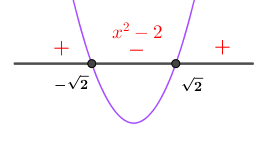
\includegraphics[width=0.4\textwidth]{imagenes/imagenes01/T01IM04.png}
			\end{figure}
				
				 *** $|x^2+3|\ge 5 \quad \to \quad x^2+3\le -5: \; x^2\le -8; \; \nexists x \qquad  \vee \qquad  x^2+3\ge 5: \; x^2\ge 2; \; x^2-2\ge 0$ De donde, procediendo como en el caso anterior para estudiar el signo de $x^2-2$ viendo previamente cuando $x^2-2=0$ y representando en $\mathbb R$ para estudiar los signos que toma $x^2-2$, usando la misma figura anterior, obtenemos como solución: $]-\infty, -\sqrt 2]\; \cup \; [\sqrt 2, \infty[$
		\end{proofw}
		
		\begin{ejre}
			Resuelve: $|x-1|+|4-2x|=4$
		\end{ejre}
		
		\begin{proofw}\renewcommand{\qedsymbol}{$\diamond$}
		
			Veamos cuando cambia el signo de los valores absolutos y representaremos en $\mathbb R$
			
			$x-1=0 \to  x=1; \qquad 4-2x=0 \to x=2$. Representamos en $\mathbb R$ los puntos $1$ y $2$ lo que nos divide el eje real en tres zonas donde analizar la ecuación como se muestra en la figura.
			
			\begin{figure}[H]
			\centering
				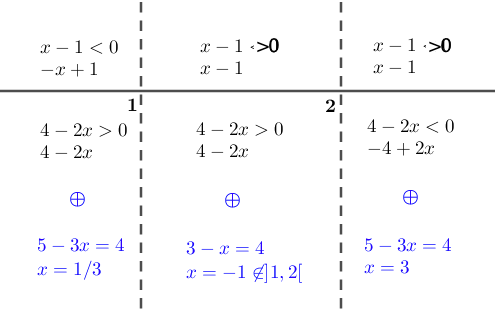
\includegraphics[width=0.85\textwidth]{imagenes/imagenes01/T01IM05.png}
			\end{figure}
			
			Soluciones:  $x=3\; $ y $\; x=1/3$.
		\end{proofw}
		
		\begin{ejre}
			Resuelve: $|x-1|\le2|x-3|$
		\end{ejre}
		
		\begin{proofw}\renewcommand{\qedsymbol}{$\diamond$}
		
			Recordemos la estrategia adoptada en la demostración del teorema 2, \emph{"para probar una desigualdad entre dos números positivos es suficiente con probar esa desigualdad para sus cuadrados"}
			
			$|x-1|\le 2|x-3| \to (x-1)^2 \le 4(x-3)^2$ Desarrollando los cuadrados y llevándolo toda a un miembro, obtenemos: $3x^2-22x+35\ge 0$.
			
			Para resolver una inecuación de segundo grado procedemos, como para resolver una inecuación de orden mayor o igual a $2$ o sobre un cociente de polinomios, buscando los ceros de la ecuación (numerador y denominador, si se trata de un cociente) y representando en el eje real donde se estudian los signos que toma el polinomio o cociente)
			$3x^2-22x+35=0 \to x=7/3 \; \vee \; x=5$. Por lo que hemos de estudiar, factorizando la expresión: $3(x-7/3)(x-5)\ge 0 \to (3x-7)(x-5)\ge 0$.
			
			En esta ocasión, vamos a resolver el problema con la ayuda de una tabla en lugar de una figura, donde estudiaremos los signos que toman los factores que forman la expresión a estudio.
			
			
			
		\begin{table}[H]
		\centering
		\begin{tabular}{|c|c|c|c|c|c|}
		\hline
	 		Intervalo & $]-\infty,7/3[$ & $7/3$ & $]7/3,5[$ & $5$ & $[5,\infty[$ \\ \hline
	 		$(3x-7)$ & $-$ & $0$ & $+$ & $+$ & $+$ \\ \hline
	 		$(x-5)$ & $+$  & $+$  & $+$ & $0$ & $-$ \\ \hline
	 		$(3x-7)(x-5)$& $-$ & $0$ & $+$ & $0$ & $-$  \\ \hline
		\end{tabular}
		\end{table}
			
		Puesto que buscábamos las zonas en que $(3x-7)(x-5)\ge 0$, la solución es: $[7/3, 5]$
			
		\end{proofw}
		
		\begin{ejre}
			Resuelve:  $\left| \dfrac {x+2}{x-6} \right| - \left| \dfrac {x-1}{x-3} \right| \le 0$ 		\end{ejre}
		
		\begin{proofw}\renewcommand{\qedsymbol}{$\diamond$}
		
			$\left| \dfrac {x+2}{x-6} \right| - \left| \dfrac {x-1}{x-3} \right| \le 0 \to \dfrac {|x+2|}{|x-6|} \le  \dfrac {|x-1|}{|x-3|} $. Como los denominadores son positivos, podemos multiplicar en cruz y el sentido de la desigualdad no varia.
			
			$|x+2|\cdot |x-3|\le |x-1| \cdot |x-6|$. Usando de nuevo la estrategia del teorema 2, 
				\emph{"para probar una desigualdad entre dos números positivos es suficiente con probar esa desigualdad para sus cuadrados"}.
			
			$(x+2)^2\cdot (x-3)^2\le (x-1)^2 \cdot(x-6)^2 \to ... \to 12x^3-72x^2+96x \le 0 $. dividiendo por 12 y factorizando (buscando ceros a la expresión), $x(x-2)(x-4)\le 0$. Veamos la tabla de signos.
			
			
	\begin{table}[H]
	\centering
	\begin{tabular}{|c|c|c|c|c|c|c|c|}
	\hline
	 Intervalos &$]-\infty, 0[$  &$0$  &$]0,2[$  &$2$ & $]2,4[$ & $4$ & $]4,\infty[$ \\ \hline
	 $x$& $-$ & 0 & + & + & + & + & + \\ \hline
 	 $x-2$& $-$ & $-$ & $-$ & 0 & + & + & + \\ \hline
 	 $x-4$& $-$ & $-$ & $-$ & $-$ & $-$ & 0 & +\\ \hline
 	 $x(x-2)(x-4)$& $-$ & 0 & + & 0 & $-$ & 0 & +\\ \hline
	\end{tabular}
	\end{table}
			
			Como nos queremos quedar con las zonas en que $x(x-2)(x-4)\le 0$, \emph{pero no podemos tomar, en ningún caso, ni el $3$ ni el $6$, que anularan los denominadores del ejercicio pedido}, la solución es:  $]-\infty, 0] \cup [2,4] \sim \{ 3 \}$



		\end{proofw}
		
		\begin{ejre}
			Resuelve $\left| \dfrac {3x+12}{x+2} \right| \ge 1$
		\end{ejre}
		
		\begin{proofw}\renewcommand{\qedsymbol}{$\diamond$}
		
			Establezcamos primero que en ningún momento podemos admitir la solución $x=-2$ puesto que anula un denominador de la inecuación de partida.
			
			$\left| \dfrac {3x+12}{x+2} \right| \ge 1 \to \dfrac {3x+12}{x+2} \le -1 \; (i)\quad \vee \quad \dfrac {3x+12}{x+2} \ge 1 \; (ii)$
			
			Resolveremos las dos inecuaciones $(i)$ e $(ii)$ por separado y tomaremos como solución la unión de las mismas, excluyendo al $-2$ si está en ellas.
 
 			Inecuación $(i): \quad \dfrac {3x+12}{x+2} \le -1 \to \dfrac {3x+12}{x+2} +1\le 0 \to \dfrac {4x+14}{x+2} \le 0$		
 			
 			Los ceros de esta expresión son $x=-7/2$ y $x=-2$ que dictarán los intervalos en que estudiar el signo del cociente. Lo vemos en la siguiente tabla:
 			
 			
 			
 			\begin{table}[H]
 			\centering
			\begin{tabular}{|c|c|c|c|c|c|}
			\hline
 			Intervalos&$]-\infty,-7/2[$  &$-7/2$  &$]-7/2,-2[$  & $-2$ &$]-2,\infty[$ \\ \hline
 			$4x+14$& $-$ & 0 & + &+  & +\\ \hline
 			$(x+2)$& $-$ & $-$  & $-$  &0  & +\\ \hline
 			$\dfrac {4x+14}{x+2}$& + & 0 & $-$ & $\nexists$ & +\\ \hline
			\end{tabular}
			\end{table}
			
			 Solución $(i):\qquad [-7/2,2[$
			
			Inecuación $(i): \quad \dfrac {3x+12}{x+2} \ge 1 \to \dfrac {3x+12}{x+2} -1\ge 0 \to \dfrac {2x+10}{x+2} \ge 0$	
			
			Los ceros de esta expresión son $x=-5$ y $x=-2$ que dictarán los intervalos en que estudiar el signo del cociente. Lo vemos en la siguiente tabla:
 			
 			
 			
 			\begin{table}[H]
 			\centering
			\begin{tabular}{|c|c|c|c|c|c|}
			\hline
 			Intervalos&$]-\infty,-5[$  &$-5$  &$]-5,-2[$  & $-2$ &$]-2,\infty[$ \\ \hline
 			$2x+10$& $-$ & 0 & + &+  & +\\ \hline
 			$(x+2)$& $-$ & $-$  & $-$  &0  & +\\ \hline
 			$\dfrac {2x+10}{x+2}$& + & 0 & $-$ & $\nexists$ & +\\ \hline
			\end{tabular}
			\end{table}
 			
 			 Solución $(i):\qquad ]-\infty,-5]\;  \cup \;  ]-2,\infty[$
 			
 			 Finalmente, la solución del problema la formarán la unión de los intervalos solución $(i)$ y $(ii)$, excluyendo, si es necesario al $\{ -2 \}$:
 			
 			 Solución:  $]-\infty, -5] \; \cup\;  [-7/2, -2[ \; \cup\;  ]-2, \infty[$
 			
		\end{proofw}
		
		
		
		\begin{ejre}
			 Resuelve: $4-|x|\le \left|\;  |2x| -6 \;   \right|$	 
		\end{ejre}
		
		\begin{proofw}\renewcommand{\qedsymbol}{$\diamond$}
				
				$4-|x|\le \left|\;  |2x| -6 \;   \right| \to 4\le \left|\;  |2x| -6 \;   \right|\; +|x|\; \to \; 4 \le 2|\;|x|-3 \; | +|x|$	
				
				\vspace{2mm} Los puntos críticos son (donde cambia el signo), en esta ocasión, 
				
				$|x|=0\to x=0; \qquad |x|-3=0 \to |x|=3 \to x=\pm 3$
				
				La siguiente tabla nos permitirá eliminar los valores absolutos en nuestra inecuación que presenta cuatro casos.
				
				
		\begin{table}[H]
		\centering
		\begin{tabular}{|c|c|c|c|c|}
		\hline
		 	Intervalos& $]-\infty, -3[$ & $[-3,0[$ & $[0,3[$ & $[3,\infty[$ \\ \hline
		 	$x$& $-$ & $-$ & + & + \\ \hline
		 	$|x|-3$& + & $-$ & $-$ & + \\ \hline
		 	casos& $i)$ & $ii)$ & $iii)$ & $iv)$ \\ \hline
		\end{tabular}
		\end{table}
			
			 $\circ$ Caso $i)\quad x\in \; ]-\infty,-3[$	
			
			$ 2|\;|x|-3 \; | +|x| \ge 4 \to 2 (\; |x|-3 \; )+(-x)\; = \; 2(-x-3)-x=-3x-6\ge 4$ 
			
			De donde: $x\le -10/3$
			
			\hspace{10mm}Sol $i):\quad ]-\infty,-10/3] \; \cap\;  ]-\infty,-3[ \; = \; ]-\infty,-10/3]$
			
			
			
			 $\circ$ Caso $ii) \quad x\in \; [-3,-0[$	
			
			$ 2|\;|x|-3 \; | +|x| \ge 4 \to 2(-\;(-x-3) \;) +(-x)=2((x+3)-x=x+6\ge 4  $
			
			De donde: $x\ge -2$
			
			\hspace{10mm}Sol $ii) \quad  [-3,0]\; \cap \; [-2,\infty[ \; = \; [-2,0[ $
			
			
			
			$\circ$ Caso $iii) \quad x\in \; [0,3[$	
			
			$ 2|\;|x|-3 \; | +|x| \ge 4 \to 2(-(x-3))+x=-x+6\ge 4 $
			
			De donde $x\le 2$
			
			\hspace{10mm} Solución $iii) \quad [0,3[ \; \cap \; ]-\infty, 2]\; = \; [0,2] $
			
			
			 $\circ$ Caso $iv) \quad x\in \; [3,\infty[$	
		
			$ 2|\;|x|-3 \; | +|x| \ge 4 \to 2(x-3)+x=3x+6\ge 4  $
			
			De donde $x\ge 10/3$
			
			\hspace{10mm} Solución $iv) \quad [3,\infty[\; \cap \; [10/3, \infty[ \; = \; [10/3, \infty[ $
			
			 Finalmente, la solución estará formada por la unión de las soluciones de los cuatro casos:
			
			\hspace{10mm} \emph{Solución final:} $]-\infty, -10/3]\; \cup \; [-2,2] \; \cup \; [10/3, \infty[$ 
			
		\end{proofw}
		
		
		\begin{ejre}
			Resuelve: $\dfrac {|x-1|-|2x+3|}{3x-4}\ge 0;\; x\neq \dfrac 4 3$
		\end{ejre}
		\begin{proofw}\renewcommand{\qedsymbol}{$\diamond$}
		
				Los puntos críticos, que hacen cambiar el signo a los argumentos del valor absoluto son, en este caso: $x-1=0 \to  x=1; \quad 2x+3=0 \to x=-3/2;\quad x\neq 4/3$ (anula el denominador).
				
				 Para resolver este problema volveremos a usar una imagen, de este modo el lector tiene dos modelos distintos de abordar el problema: en forma de tabla o de gráfico-imagen.
				
			\begin{figure}[H]
			\centering
				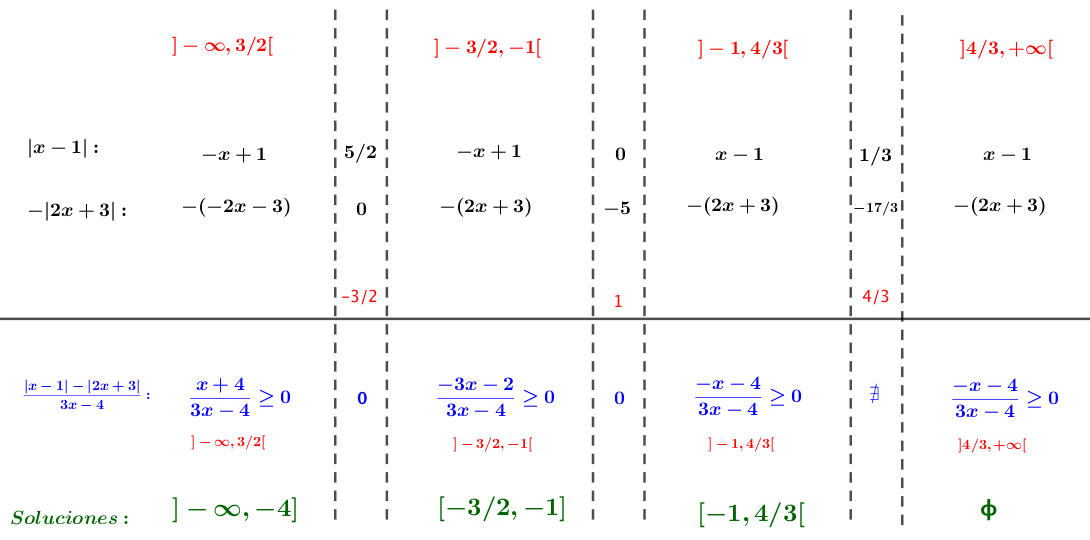
\includegraphics[width=1\textwidth]{imagenes/imagenes01/T01IM06.png}
			\end{figure}
			
			 La solución final es $\; ]-\infty, -4] \cup [-3/2,4/3[$
				
		\end{proofw}
		
	    \emph{Nota:}  $\emptyset$ es símbolo del conjunto vacío.
		
		
		
		\begin{ejre} $\divideontimes$.
			Demuestra la fórmula del \textbf{Binomio de Newton:}	
			\label{ejre:binomio-newton}
			\begin{equation}
				\forall a,b \in \mathbb R,\; \forall n \in \mathbb N: \quad (a+b)^n = \sum_{k=0}^n {\left( \begin{matrix} n \\ k \end{matrix}  \right)a^{n-k}\; b^k}
			\end{equation}
		\end{ejre}
		
		\begin{proofw}\renewcommand{\qedsymbol}{$\diamond$}
		
				Aplicaremos el \emph{Principio de inducción}: para $n=1$ la igualdad del enunciado se cumple  trivialmente.
				
				Supongamos la igualdad verdadera para $n$, entones, para $n+1$ tendremos (recordando las propiedades de los números combinatorios):
				
				\hspace{25mm}$(a+b)^{n+1}=(a+b)(a+b)^n=(a+b)\; \sum_{k=0}^n {\left( \begin{matrix} n \\ k \end{matrix}  \right)a^{n-k}\; b^k}=$
				
			    \hspace{25mm}$={\sum_{k=0}^n \left( \begin{matrix} n \\ k \end{matrix}  \right)a^{n+1-k}\; b^k}+\sum_{k=0}^n {\left( \begin{matrix} n \\ k \end{matrix}  \right)a^{n-k}\; b^{k+1}}$
				
				\hspace{25mm}$ =\sum_{k=0}^n {\left( \begin{matrix} n \\ k \end{matrix}  \right)a^{n+1-k}\; b^k}+\sum_{k=1}^{n+1} {\left( \begin{matrix} n \\ k-1 \end{matrix}  \right)a^{n+1-k}\; b^{k}} $
				
				\hspace{25mm} $ = a^{n+1}+b^{n+1}+\sum_{k=1}^n 
				\left[ \left( \begin{matrix} n \\ k \end{matrix}  \right) + \left( \begin{matrix} n \\ k-1 \end{matrix}  \right)    \right]a^{n+1-k}\; b^k=$
				
				\hspace{25mm} $=\sum_{k=0}^{n+1} {\left( \begin{matrix} n+1 \\ k \end{matrix}  \right)a^{n+1-k}\; b^k}$
				
		\end{proofw}
		
		
		
		\begin{ejre} $\divideontimes$.
			Demuestra que: $1^3+2^3+3^3+\; ...\; n^3= [n(n+1)/2]^2$
		\end{ejre}
		
		\begin{proofw}\renewcommand{\qedsymbol}{$\diamond$}
		
			Aplicamos el \emph{principio de inducción} y comprobamos, primero, que la fórmula se cumple para $n=1$, lo cual es obvio. Suponemos que se cumple para $n$ y veamos que ocurre para $n+1$
			
				 $1^3+2^3+3^3+\; ...\; n^3 \; \; +\; (n+1)^3\; =  [n(n+1)/2]^2 \; \; +(n+1)^3=$
				
				 $=  \left( \dfrac {n(n+1}{n} \right)^2 + (n+1)^3=\dfrac {(n^2+n)^2+4(n+1)^3}{4}= \frac 1 4 [n^4+6n^3+13n^2+12n+4]=$
				
				  $=\frac 1 4 [n^4+6n^3+13n^2+12n+4]=$factorizando por Ruffini: $=(n+1)^2(n+2)^2/4$
				
				=[que podemos escribir como] $=\left[ \dfrac {(n+1)(n+2)}{2} \right]^2$, que es la formula general al sustituir $n+1$ por $n$.
		\end{proofw}
		
		\begin{ejre} $\divideontimes$.
			Demostrar que no existe un número racional mínimo mayor que cero.
		\end{ejre}
		
		\begin{proofw}\renewcommand{\qedsymbol}{$\diamond$}
		
		En la demostración por reducción al absurdo se comienza por asumir lo contrario y nuestra tesis sería: existe un número racional mínimo mayor que cero: $r_0$.

		Ahora tomemos $x = r_0/2$. Por lo tanto $x$ es un número racional mayor que cero, y $x<r_0$. Eso es un absurdo, pues contradice la hipótesis de partida de que $r_0$ era el número racional mínimo. Por lo tanto se debe concluir que la proposición asumida como cierta: $``$hay un número racional mínimo mayor que cero$"$ es falsa.
		\end{proofw}
		
		\begin{ejre} $\divideontimes$.
			Demostrar que hay infinitos números primos.
		\end{ejre}
		
		\begin{proofw}\renewcommand{\qedsymbol}{$\diamond$}
		
		Existen numerosas demostraciones sobre que existen infinitos números primos, la primera de la que se tiene constancia es de Euclides, donde queda demostrado mediante 	\emph{Reductio ad absurdum} en la Proposición 20 del libro IX de Elementos (Hay más números primos que cualquier cantidad propuesta de números primos).
		
		Partiendo de suponer que lo cierto es lo contrario, por lo cual nuestra tesis quedara: $``$Los números primos son finitos$"$, entonces tenemos $n$ números primos que seran $P=p_1,\; p_2,\; ...,\; p_n$

		Entonces se toma ahora el siguiente número: $m=p_1 \cdot p_2 \cdot \; ...\cdot\; p_n+1$

		Tenemos que $m$ es el producto de todos los primos más uno, y $m$ no es un número primo, pues no se encuentra en la lista anterior, luego ha de ser un número compuesto.

 		Si dividimos $m$ por cualquiera de los primos que tenemos, todos ellos en $P$, nos da resto uno. Para que $m$ sea compuesto debería ser divisible por otro número que no está en nuestra lista de todos los números primos.
		
		Entonces llegamos a una contradicción de nuestra tesis $``$Los números primos son finitos$"$ que es falsa, por lo cual s existen infinitos números primos.
		\end{proofw}
		
		\begin{ejre} $\divideontimes$.
			Dados 5 puntos cualesquiera dentro de un triángulo equilátero de lado 2, al menos dos de ellos están a una distancia, el uno del otro, menor que 1.
		\end{ejre}
		
		\begin{proofw}\renewcommand{\qedsymbol}{$\diamond$}
		
			Está claro que por estar dentro de un triángulo equilátero de lado 2, cualesquiera dos puntos, de los cinco que hemos elegido, están a una distancia menor que 2, pero ?`podemos afirmar que siempre habrá dos de ellos que están a una distancia menor que 1?

			Para aplicar el principio del palomar se consideran los puntos medios de los lados del triángulo y se unen con segmentos, lo cual divide al triángulo en cuatro triangulitos equiláteros de lado 1. Como son cuatro triángulos de lado 1 (que serán nuestros palomares) y cinco puntos (que serán nuestras palomas), entonces habrá dos puntos en el mismo triángulo equilátero de lado 1, y esos dos están a una distancia menor que 1.
			
			\begin{figure}[H]
			\centering
				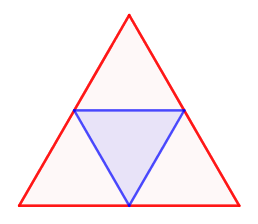
\includegraphics[width=0.3\textwidth]{imagenes/imagenes01/T01IM07.png}
			\end{figure}
		\end{proofw}
		
		%\clearpage.   corte de página
		
	
	\subsection{Ejercicios Propuestos}
	
		
		\begin{enumerate}[1).-  ]
		\item $4x+1<2x \qquad \qquad$ 
		
		\rightline{\textcolor{gris}{Solución: $]-\infty, -1/2[$}}
	
		\item $2x-1\ge0$
		 
		\rightline{\textcolor{gris}{Solución: $[1/2,\infty[$}}
		
		\item $\dfrac {2x+1}{x+3}>3$
		
		\rightline{\textcolor{gris}{Solución: $]-8,-3[$}}
	
		\item $x^3-3x^2-10x+24<0$
		
		\rightline{\textcolor{gris}{Solución: $]-\infty, -3[ \cup ]2,4[$}}
		
		\item $|x+2|\ge 5$
		
		\rightline{\textcolor{gris}{Solución: $]-\infty, -7] \cup [3,\infty[$}}
		
		\item $ \left| \dfrac 2 x -3 \right| \le 5$
		
		\rightline{\textcolor{gris}{Solución: $]-\infty,-1]\cup [1/4, \infty[$}}
		
		
		\item $ \left| \dfrac {2x-1} x \right| > 2$
			
		\rightline{\textcolor{gris}{Solución: $ ]-\infty, 0[\cup]0,1/4[ $}}
		
		\item $|x|+|x+1|=2$
		
		\rightline{\textcolor{gris}{Solución: $\{ -3/2;\; 1/2 \}$}}
		
		\item $|x-2|^2-5|x-2|+6=0$
		
		\rightline{\textcolor{gris}{Solución: $\{ -1, 0, 4, 5  \}$}}
		
		\item $|x-2|-|x+2|=|x|$
		 
		\rightline{\textcolor{gris}{Solución: $ \{ -4,0 \}$}}
		
		\item $|x^2+3x|=|x+3|$
		
		\rightline{\textcolor{gris}{Solución: $\{ -3, -1, 1 \} $}}
		
		\item $\dfrac {|x^2-16|}{x+4}\le \dfrac {x^2}{|x-1|}$
		
		\rightline{\textcolor{gris}{Solución: $ ]-\infty, -4[ \cup [4/5, 1[\cup ]1, \infty[  $}}
		
		\item $ \left|\dfrac {3|x|-x}{x+1} \right| < \dfrac 1 {x+1}$
		
		\rightline{\textcolor{gris}{Solución: $ ]-1/4, 1/2[$}}
		
		
		\end{enumerate}

		
		
	$\divideontimes$ AMPLIACIÓN: Aplicaciones \emph{curiosas}. \label{curiosidades1}
		
		\begin{multicols}{2}
			
		
		$\sqrt{12+\sqrt{12+\sqrt{12+...}}}=x$  
		
		
		$x^{x^{x^{...}}}=2$
		
		
		$\sqrt {x \sqrt {x \sqrt {x \sqrt {...}}}}=?$
		
		$7-\dfrac {12}{7-\dfrac {12}{7-\dfrac {12}{7-\dfrac {7}{12- ...}}}}=x$
		
		$\dfrac {1}{1+2\cdot \left( \dfrac {1}{1+2\cdot \left( \dfrac {1}{1+ ...} \right)} \right)}=x$
		
		$\sqrt{5+\sqrt{5-\sqrt{5+\sqrt{5- ...}}}}=\dfrac {a+\sqrt{b}}{c} \to \mbox{calcula: } a^2+b^2+c^2$
		
		\end{multicols}
		
		
		\textcolor{gris} {Resolvemos uno de estos problemas, p.e.:}
		
		\textcolor{gris} {$\dfrac {1}{1+2\cdot \left( \dfrac {1}{1+2\cdot \left( \dfrac {1}{1+ ...} \right)} \right)}=x \to x=\dfrac {1}{1+2[x]} \to x+2x^2=1;\; 2x^2+x-1=0$}
		
		\textcolor{gris} {$\to x=1 \vee x=-2 \mbox{ (sin sentido)}$ }


\vspace{4mm}

\textit{para la redacción de este capítulo me ha sido de gran ayuda los apuntes de catedrático de apuntes del catedrático F.J. Pérez Gonzalez, catedrático del departamento de Análisis Matemático de la Universidad de Granada. Muchas gracias por compartir tu saber.}


\chapter{Funciones}	

	\section{Función real de variable real}
	
		
Las funciones son las herramientas principales para la descripción matemática de una situación real. Todas las fórmulas de la Fí­sica no son más que funciones: expresan cómo ciertas magnitudes (por ejemplo el volumen de un gas) dependen de otras (la temperatura y la presión). El concepto de función es tan importante que muchas ramas de la matemática moderna se caracterizan por el tipo de funciones que estudian. No es de extrañar, por ello, que el concepto de función sea de una gran generalidad. Además, se trata de uno de esos conceptos cuyo contenido esencial es fácil de comprender aunque difí­cil de formalizar.

	En matemática, se dice que una magnitud es función de otra si el valor de la primera depende del valor de la segunda. Por ejemplo el área $A$ de un cí­rculo es función de su radio $r$ (el valor del área es proporcional al cuadrado del radio, $A = \pi\cdot r^2$). Del mismo modo, la duración $t$ de un viaje en tren entre dos ciudades separadas por una distancia $d$ de $150\;  km$ depende de la velocidad $v \; km/h$ a la que se desplace el tren (la duración $t$ es inversamente proporcional a la velocidad, $150 / v$). A la primera magnitud (el área, la duración) se la denomina \emph{variable dependiente}, y la magnitud de la que depende (el radio y la velocidad) es la \emph{variable independiente}.

	La palabra función fue introducida en Matemáticas por Leibniz, que utilizaba este término para designar cierto tipo de fórmulas matemáticas. Más tarde se vio que la idea de función de Leibniz tení­a un alcance muy reducido y, posteriormente, el significado de la palabra función fue experimentando generalizaciones progresivas. Actualmente, la definición de función es esencialmente la siguiente:
	
	\begin{defi}
		En análisis matemático, el concepto general de función, aplicación o mapeo se refiere a una regla que asigna a cada elemento de un primer conjunto $A$ (llamado \emph{Dominio o Campo de Existencia} de la función) un \underline{único elemento} de un segundo conjunto $B$ (llamado \emph{Recorrido o Rango} de la función).
		
		 Obsérvese que una función son tres cosas. el conjunto $A$ sobre el que actíúa la función, el conjunto $B$ en el que toma valores y la regla que la define. 
	
		 Esquemáticamente: $f: A \to B \; / \; \forall x \in A \leadsto \exists ! \; y=f(x) \in B$
		
	\end{defi}
	
		 En este curso nos van a interesar las \emph{funciones reales} ($B \in \mathbb R$) \emph{de variable real} ($A \in \mathbb R$).
	
	%\begin{figure}[H]
		%\centering
		%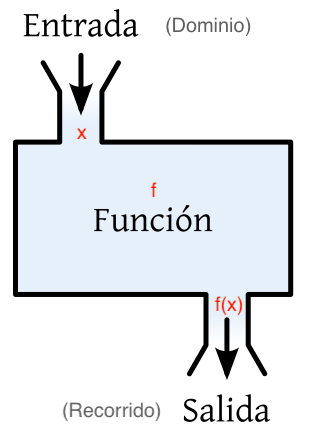
\includegraphics[width=0.3\textwidth]{imagenes/imagenes02/T02IM01.png}
		%\caption{Podemos considerar una función como una especie de máquina matemática que transforma unos números reales en otros.}
	%\end{figure}
	
	\begin{figure}[H]
		\centering
		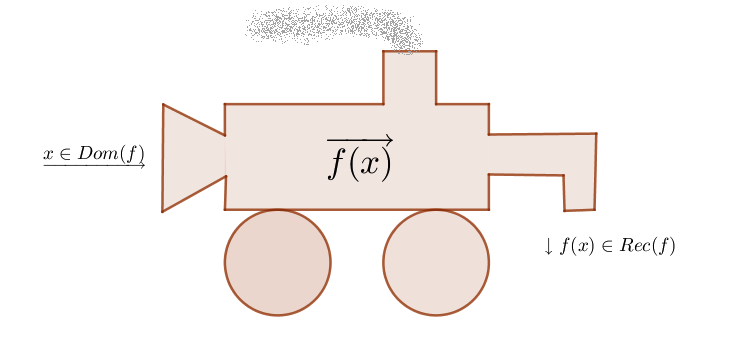
\includegraphics[width=0.7\textwidth]{imagenes/imagenes02/T02IM01b.png}
		\caption{Podemos considerar una función como una especie de máquina matemática que transforma unos números reales en otros.}
	\end{figure}
	

		
	 El dominio de una función puede restringirse según el contexto. Por ejemplo, el dominio de la función de área dado por $A = \pi r^2$ solamente permite que los radios $r$ sean positivos (ya que es una distancia). Cuando definimos una función $y =f(x)$ con una fórmula y el dominio no se da explí­citamente o está restringido por el contexto, se supone que es el máximo conjunto de valores de $x$ reales para los que la fórmula da valores reales de $y$; este dominio se llama dominio natural. Si queremos restringir el dominio de alguna manera, debemos especificarlo.
	\begin{multicols}{2}
	Los dominios naturales de las funciones polinómicas es $\mathbb R$, para las funciones racionales hay que excluir de $\mathbb R$ los números que anulen su denominador, las funciones radicales, de í­ndice par, el domino natural estará formado por todos los números $\mathbb R$ que hacen que el radicando sea no-negativo (desigualdad). Las funciones logarí­tmicas solo se pueden calcular si el argumento es positivo. Las tangentes no están definidas para múltiplos impares de $\pi/2$, etc.
	
		\begin{figure}[H]
			\centering
			\includegraphics[width=0.35
			\textwidth]{imagenes/imagenes02/xiste02.png}
		\end{figure}
		\end{multicols}
	 \begin{defi}
	Llamamos \emph{gráfica} de una función $f$ a los puntos del plano $(x,y)$ tales que $y=f(x)$. Más concretamente:
	
	$G(f)=\{ (x,y)\in 	\mathbb R^2 \; / \; x\in Dom(f) \wedge y=f(x) \in Rec(f)   \}$	
	\end{defi}
	
	 La gráfica de una función nos da mucha información. A partir de la gráfica podemos saber:
	
	\begin{itemize}
		\item \emph{$Dom(f)$} se puede obtener sin más que ``proyectar'' la función sobre el eje $OX$. La zona sombreada constituye el dominio de la misma. (En rojo en la figura \ref{fig:dom-rec})
		\item \emph{$Rec(f)$} se puede obtener sin más que ``proyectar'' la función sobre el eje $OY$. La zona sombreada constituye el recorrido de la misma. (En verde en la figura \ref{fig:dom-rec})

		\item \emph{Estrategia de la vertical:} sabemos que una curva es la gráfica de una función matemática si al trazar lí­neas verticales, éstas cortan ninguna o \underline{una sola vez} a la curva. (Lí­neas grises en la figura \ref{fig:dom-rec})
		
	\end{itemize}

	\begin{figure}[H]
		\centering
		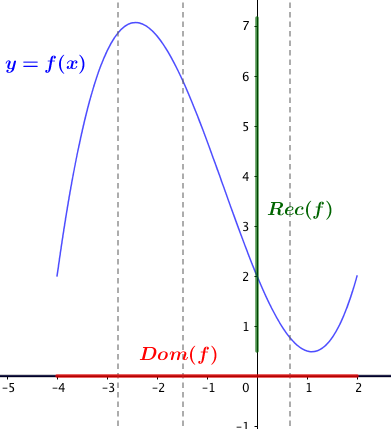
\includegraphics[width=0.5\textwidth]{imagenes/imagenes02/T02IM02.png}
		\caption{Gráfica de una función (azul), con su dominio (rojo) y recorrido (verde). Las lí­neas grises son la prueba de la vertical que asegura que $f$ es una función.}
		\label{fig:dom-rec}
	\end{figure}
		
	\begin{defi}[Igualdad de funciones]. 
	
	$f=g$ cuando $Dom(f)=Dom(g)\; $ y $\; f(x)=g(x),; \forall x\; $ en el dominio común.
		
	\end{defi}
		
	Es decir, dos funciones con la misma regla que las defina (fórmula) pero que tengan dominios diferentes se consideran funciones distintas.	
		
	
	\section{Operaciones con funciones}
		
		\begin{defi}{Funciones Elementales}
		
		En matemáticas, una \emph{función elemental} es una función construida a partir de una cantidad finita de funciones elementales fundamentales y constantes mediante operaciones racionales (adición, sustracción, multiplicación y división) y la composición de funciones usando exponenciales, logarí­tmicas, potenciales, constantes y las funciones trigonométricas y sus inversas, todas consideradas dentro del grupo de funciones elementales fundamentales.
			
		\end{defi}
		
		 Son \emph{funciones elementales fundamentales}:
		
		\begin{enumerate}
			\item Función constante: $f(x)=c,\; c\in \mathbb R$
			\item Función identidad: $f(x)=x$
			\item Función potencial: $f(x)=x^k,\; k\in \mathbb R \sim \{0\}$. Este tipo de funciones comprende a la función cuadrática $x^2$, la cúbica $x^3$, la raí­z $\sqrt x = x^{1/2}$, etc.
			\item Función exponencial: $f(x)=a^x,\; x\in \mathbb R,\; a\in \mathbb R^+ \sim \{ 1 \}$
			\item Función logarí­tmica: $f(x)=\log_a (x),\; x\in \mathbb R^+ ,\; a\in \mathbb R^+ \sim \{ 1 \}$
			\item Funciones trigonométricas: $f(x)=\sin x\; ; \quad f(x)=\cos x\; ; \qquad f(x)=\tan x \;  (x\neq (2k+1) \cdot 	\frac {\pi} {2}, \; k\in \mathbb Z)$
			\item Funciones trigonométricas inversas: $f(x)=\arcsin (x)\; (x\in [-1,1]); \quad f(x)=\arccos (x)\; (x\in [-1,1]); \quad f(x)=\arctan (x)\; (\forall x \in \mathbb R) $
		\end{enumerate}
		
		\begin{defi}{Suma, producto y cociente de funciones}.
			
			
			Dadas $f,g: A \to \mathbb R$, se define:
			
			\begin{itemize}
				\item producto por un número: $(kf)(x)=k\cdot f(x),\; k\in \mathbb R$, se representa por $kf$
				\item suma: $(f+g)(x)=f(x)+g(x)$, se representa por $f+g$
				\item producto: $(f\cdot g)(x)=f(x)\cdot g(x)$, se representa por $fg$
				\item cociente: $(f/g)(x)=f(x)/g(x),\; x\in A\; / \; g(x)\neq 0$, se representa por $f/g$
			\end{itemize}
			
		\end{defi}
		
		Obviamente un número se puede multiplicar por uno dado si existe el primero, dos números se pueden sumar, restar o multiplicar si ambos existen y, por último, dos números se pueden dividir si, existiendo ambos, el divisor es distinto de cero. Es por ello que:
		
		$Dom(k\cdot f)=Dom(f); \quad Dom(f+g)=Dom(f-g)=Dom(f\cdot g)=Dom(f) \cap Dom(g); \quad Dom(f/g)=Dom(f) \cap Dom(g)\sim \{x/g(x)=0 \}$

	\begin{prop} $\forall \; f,g,h : A \to \mathbb R\; $ se verifican las siguientes propiedades:
	
		\begin{enumerate}
			\item Asociativas: $(f+g)+h=f+(g+h); \qquad (fg)h=f(gh) $
			\item Conmutativas: $f+g=g+f; \qquad fg=gf$
			\item Distributiva: $(f+g)h=fh+gh$
		\end{enumerate}
	\end{prop}
	\begin{proof} La demostración es inmediata pues se reduce a las propiedades de los números reales.	
	\end{proof}

	\subsection{Composición de funciones y función inversa}
	
	

	\begin{defi}{Composición de funciones}.
	
	Sean $f:A \to \mathbb R, \; g:B \to \mathbb R$, tales que $f(A) \subset B$. En este caso, la función $h:A \to \mathbb R$ dada por $h(x)=g \left( f(x) \right)$ se llama \emph{composición de $g$ con $f$} y se representa por $h=g \circ f$. Es importante observar que la composición $h=g \circ f$ está definida solo si la imagen de $f$ está contenida en el dominio de $g$.
	
	
	La composición de funciones es asociativa, pero no-conmutativa.
	
	
	\begin{itemize}
		\item Asociativa: $(f \circ g) \circ h =f \circ (g \circ h) $
		\item No-Conmutativa: $f \circ g \neq g \circ f$
	\end{itemize}
		
	\end{defi}
	
	\begin{figure}[H]
		\centering
		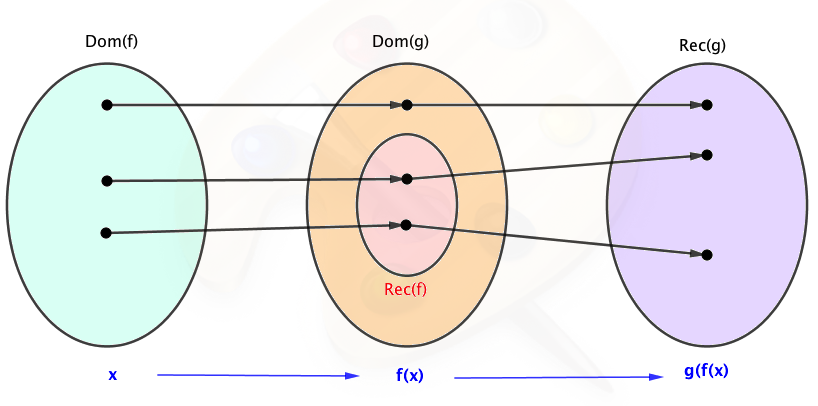
\includegraphics[width=0.6\textwidth]{imagenes/imagenes02/T02IM03.png}
		\caption{Composición de funciones.}
	\end{figure}
		

		\begin{defi}{Funciones Inyectivas}.
		
		 Se dice que $f:A\to \mathbb R$ es \emph{inyectiva} en un conjunto $C \subset A$ si en puntos distintos de $C$ toma valores distintos, es decir, si $\forall x,y \in C,\; x\neq y \to f(x) \neq f(y)$ 	
	
		\end{defi}
		\emph{Prueba de la lí­nea horizontal}. Dada la gráfica de una función, si al trazar lí­neas horizontales, paralelas al eje $OX$ cortamos más de una vez a la función, entonces no será inyectiva.
		
		\begin{figure}[H]
			\centering
			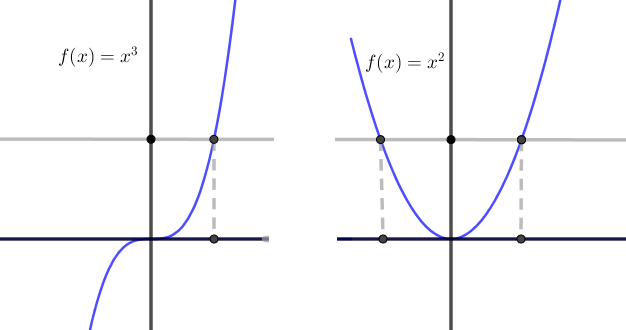
\includegraphics[width=0.6\textwidth]{imagenes/imagenes02/T02IM04.png}
			\caption{Prueba de la lí­nea horizontal: la primera función sí­ es inyectiva y la segunda no, la lí­nea horizontal corta más de una vez a la gráfica.}
		\end{figure}
		
		La importancia de la inyectividad está en que cuando resolvamos ecuaciones basadas en funciones inyectivas, la solución será única ($f(x)=x^2$ no es inyectiva, al resolver $x^2=4 \to x=|2|=\pm 2$, en cambio, $g(x)=x^3$ sí­ es inyectiva, por ello, $\sqrt [3] {-8}=-2$, tiene solución única). También es importante la inyectividad de una función a la hora de calcular su función inversa, como veremos a continuación.
		
		\begin{defi} {Función inversa} (de una función inyectiva).
		
		
			Si $f:A \to \mathbb R$ es una \emph{función inyectiva}, puede definirse una nueva función $f^{-1}:B=f(A) \to 	\mathbb R$, que llamaremos \emph{función inversa} de $f$, que $\forall y\in B=f(A), \; \exists ! x\in A: \; f(x)=y$. Equivalentemente, $f^{-1} \left(  f(x) \right)=x, \; \forall x \in A$ y también $f \left( f^{-1}(y)  \right) = y,\; \forall y \in B=f(A)$.

		\end{defi}
		
		Para calcular la inversa de una función (lo veremos en los ejercicios resueltos) escribiremos $y=f(x)$, cambiaremos las $x$ por las $y$ y, por último, despejaremos la $y=f^{-1}(x).$
		
		 Considerando una función (inyectiva) como una máquina que transforma unos números en otros, la función inversa serí­a como conectar la máquina al revés. Todo ello hace que se intercambien los papeles $x\leftrightarrow y$. En la gráfica de la función identidad $y=f(x)=x$ es en la que tanto $x$ como $y$ juegan el mismo papel, por ello \emph{las gráficas de $f$ y $f^{-1}$} serán \emph{simétricas} respecto de la bisectriz del primer y tercer cuadrante ( que es la gráfica de la función identidad $y=f(x)=x=I(x)\,)$.
		
		
		
		\begin{prop}{Propiedades de la función inversa.}
		\label{prop:funcion-inversa}
		\begin{itemize}
			
			\item $Dom(f^{-1})=Rec(f); \quad Rec(f^{-1})=Dom(f)$
			\item $ \left( f^{-1} \right) ^{-1} (x)=f(x) $
			\item $ (f \circ f^{-1}) (x)= I(x)=x; \quad (f \circ f^{-1})(x)=I(x)=x$
			\item $ \left( f \circ g   \right)^{-1}(x)=\left(  g^{-1}\circ f^{-1} \right)(x) $	
			
			\footnotesize{Esta última curiosa propiedad es caracterí­stica de las operaciones no conmutativas, en el producto de matrices (invertibles), que es no conmutativo, también se da de forma similar: $(A\cdot B)^{-1}=B^{-1}\cdot  A^{-1}$}
		\end{itemize}	
		
		\end{prop}
		
		\begin{proof}
			La demostración de estas propiedades algebraicas de la función inversa es la aplicación directa de la definición.
		\end{proof}
		
		\emph{Nota:} No hay que confundir \emph{función inversa} $f^{-1}(x)$, que es cuando la función `marcha al revés'  con la \emph{inversa de una función} que es $\dfrac 1 {f(x)}$.
		

		\begin{figure}[H]
			\centering
			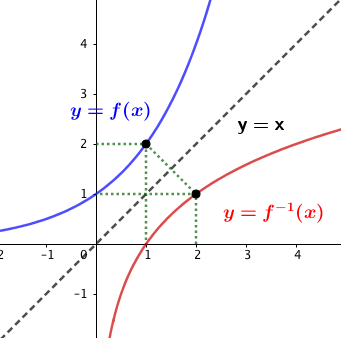
\includegraphics[width=0.3\textwidth]{imagenes/imagenes02/T02IM05.png}
			\caption{Gráficas de una función y su función inversas, simétricas respecto de $y=x$.}
		\end{figure}
		
		\textbf{Funciones arco.}
		
		 La función $y=\sin x$ es no-inyectiva, pero si nos quedamos con un tramo en que sí­ lo es, $[-\pi/2, \pi/2]  \; \;  \underrightarrow { \sin x } \; \;  [-1,1]$ podemos tomar su función inversa: $y=\arcsin x: [-1,1] \to [-\pi/2, \pi/2] $
		
		Se verifica que $\quad \sin (\arcsin x)=x; \qquad \arcsin (\sin x)=x$
		
		 Lo mismo para la función $y=\cos x$ es no-inyectiva, pero si nos quedamos con un tramo en que sí­ lo es, $[0, \pi]  \; \;  \underrightarrow { \cos x } \; \;  [-1,1]$ podemos tomar su función inversa: $y=\arccos x: [-1,1] \to [0, \pi] $
		
		Se verifica que $\quad \cos (\arccos x)=x; \qquad \arccos (\cos x)=x$
		
		
		
		\begin{figure}[H]
			\centering
			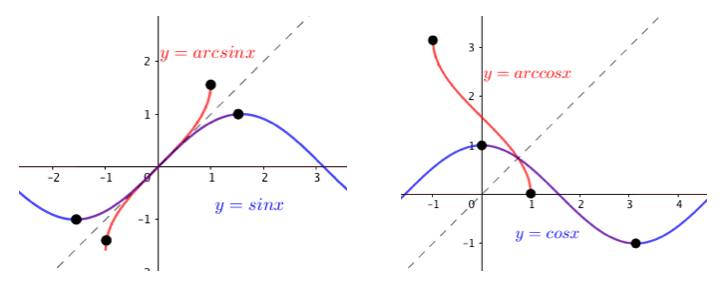
\includegraphics[width=0.8\textwidth]{imagenes/imagenes02/T02IM06.png}
			\caption{Funciones arco: arco seno y arco coseno y zonas de inyectividad de seno y coseno..}
		\end{figure}
		
		La función tangente es periódica, de periodo $\pi$. Tomando uno de estos periodos en que la tangente es inyectiva: $[-\pi/2, \pi/2] \; \;  \underrightarrow { \tan x } \; \; \mathbb R $, podemos tomar su función inversa: $y=\arctan x: \mathbb R \to [-\pi/2, \pi/2]$
		
		Se verifica que $\quad \tan (\arctan x)=x; \qquad \arctan (\tan x)=x$
		
		
		\begin{figure}[H]
			\centering
			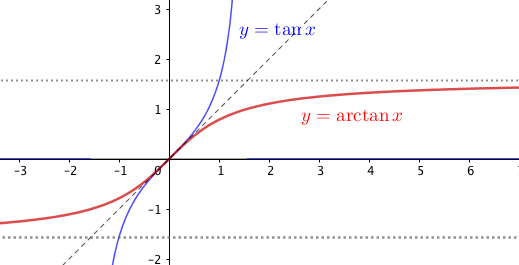
\includegraphics[width=0.6\textwidth]{imagenes/imagenes02/T02IM07.png}
			\caption{Función arco tangente.}
		\end{figure}
		
		

		
		\section{Transformaciones elementales de funciones}
		\subsection{Traslaciones}
		\begin{itemize}
			\item Traslaciones Verticales: $y=f(x)+k$
			
			Desplaza a la función $f(x)$ $k$ unidades hacia arriba si $k>0$ o hacia abajo si $k<0$
			
			\item Traslaciones Horizontales: $y=f(x+h)$
			
			Desplaza a la función $f(x)$ $h$ unidades hacia la izquierda si $h>0$ o hacia la derecha si $h<0$
		\end{itemize}
		
		\begin{figure}[H]
			\centering
			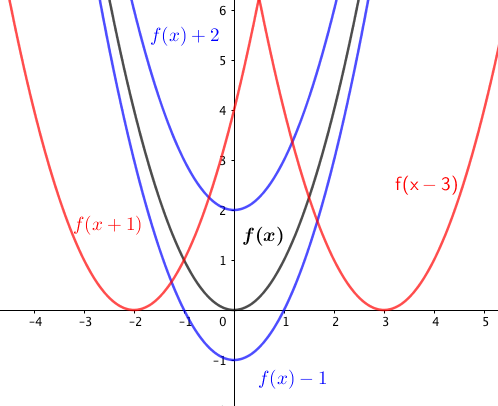
\includegraphics[width=0.4\textwidth]{imagenes/imagenes02/T02IM08.png}
			\caption{Traslaciones.}
		\end{figure}
		
		\subsection{Simetrí­as}
		
		\begin{itemize}
			\item $y=-f(x)$: Simetriza a la función respecto del eje $OX$
			\item $y=f(-x)$: Simetriza a la función respecto del eje $OY$
		\end{itemize}
		
		\begin{figure}[H]
			\centering
			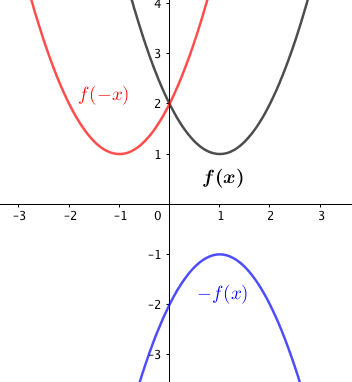
\includegraphics[width=0.3\textwidth]{imagenes/imagenes02/T02IM09.png}
			\caption{Simetrí­as.}
		\end{figure}
		
			\begin{defi} Paridad de una función.
			
			 Dada $f(x)$, calculamos $f(-x)$ y pueden pasar tres cosas:	
			
			\begin{itemize}
				\item [-] $f(-x)=f(x) \to $ función PAR, simétrica respecto de $OY$
				\item [-] $f(-x)=-f(x) \to $ función IMPAR, simétrica respecto de $OX$
				\item [-] Otra cosa $\to$ función sin paridad.
			\end{itemize}
			\end{defi}
			
		\begin{figure}[H]
		\centering
		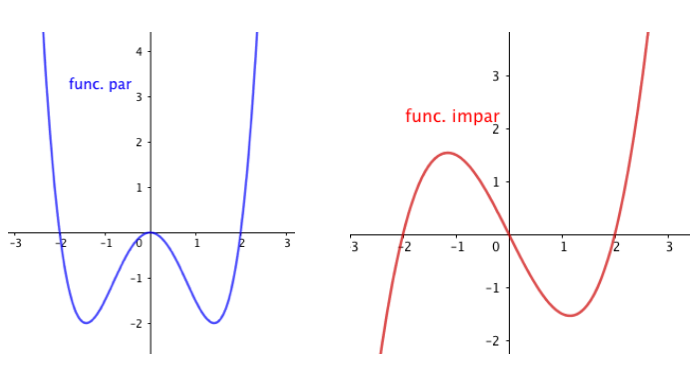
\includegraphics[width=0.5\textwidth]{imagenes/imagenes02/T02IM10.png}
		\caption{Paridad.}
		\end{figure}
		

		\subsection{Estiramientos y contracciones}
		\begin{itemize}
			\item Verticales: $y=b f(x)$. Para $b>1$ se produce un estiramiento vertical, para $0<b<1$ una contracción vertical.
			\item Horizontales: $y=f(ck)$. Para c>1 se produce un estiramiento horizontal, para $0<c<1$ una contracción horizontal.
		\end{itemize}
		
		\begin{figure}[H]
			\centering
			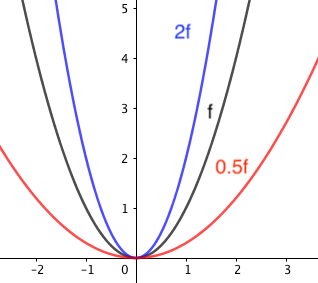
\includegraphics[width=0.3\textwidth]{imagenes/imagenes02/T02IM11.png}
			\caption{Estiramientos y contracciones verticales.}
		\end{figure}
		
		\subsection{Funciones monotónas, acotadas y periódicas}
		
		\begin{defi}Funciones monótonas.
		
		 Se dice que $f:A \to \mathbb R$ es monótona creciente (decreciente) en un conjunto $C\subset A$ si $\forall x_1, x_2 \in C$ con $x_1\le x_2$, entonces $f(x_1)\le f(x_2)$. ($f(x_1)\ge f(x_2)$, para decreciente).
		\end{defi}
		
		\begin{defi} Funciones acotadas.
		
		Una función $f(x)$ está acotada en un conjunto $A$ si existe un número real $K$ tal que $|f(x)|\le K,\; \forall x \in A$	
		
		Si no se especifica el conjunto $A$ se supone que es todo su $Dom(f)$ y, en tal caso, la gráfica de $f$ estará contenida en una banda horizontal definida por las rectas $y=k$ e $y=-k$
		
		\end{defi}
		
		\begin{defi} Funciones periódicas.
		
		Una función es periódica	 si existe un número real $T\neq 0$ tal que $f(x+T)=f(x)$. A este número $T$ se le llama periodo.
		
		Las funciones $\sin x$ y $\cos x$ son periódicas de periodo $2\pi$. La función $\tan x$ tiene periodo $\pi$.
		\end{defi}

		\begin{figure}[H]
			\centering
			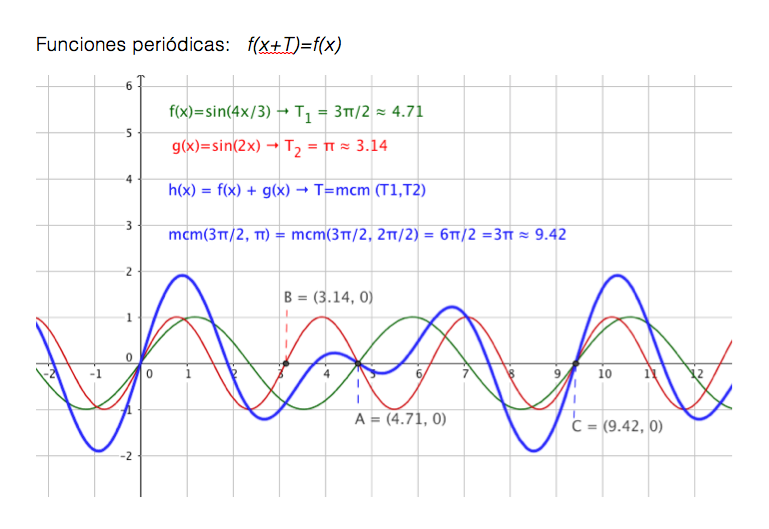
\includegraphics[width=0.6\textwidth]{imagenes/imagenes02/T02IM25.png}
			\caption{$\divideontimes$ Función periódica}
					\end{figure}
		
		\section{Otro tipo de funciones}
		
		\subsection{Funciones definidas a trozos}
		
		\begin{defi}{Función definida a trozos}.
		
		$f: A \to B$. Supongamos que A puede representarse como una unión de conjuntos disjuntos, con $A_i: \; A=\bigcup_{i=1}^{n}{{A}_{i}} $, entonces f es una \underline{función definida a trozos} si $\forall x \in A_i:\; f(x)=f_i(x),\; 1\le x \le n$
			
		\end{defi}

		
		 La función más famosa que ya vimos en el capí­tulo anterior fue el valor absoluto:
		
		\begin{equation*}
		|x|=
		\begin{cases} 
		\;\;  x &\mbox{if } x\ge 0 \\ 
		\; -x & \mbox{if } x<0 
		\end{cases}
		\end{equation*}
	
		 Otras funciones interesantes y también definidas a trozos son la \emph{parte entera} y la \emph{parte decimal} o mantisa de un número real, definidas como:
		 
		 Parte entera: $\left\lfloor x \right\rfloor = $ entero anterior o igual a x.
		 
		 Parte decimal: $Dec(x)=x-\left\lfloor x \right\rfloor$
		 
		 Vemos sus gráficas en la siguiente imagen.
		 
		\begin{figure}[H]
			\centering
			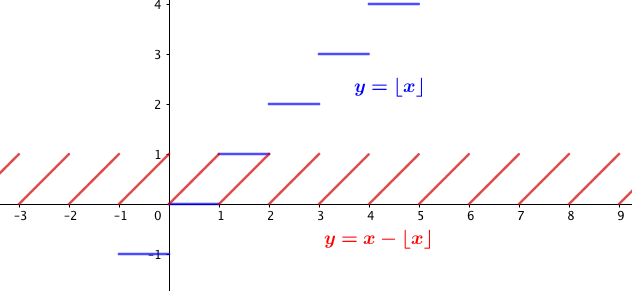
\includegraphics[width=0.7\textwidth]{imagenes/imagenes02/T02IM12.png}
			\caption{Funciones parte entera y parte decimal}
		\end{figure}
		
		 \begin{multicols}{2}
		 Otra función definida a trozos que merece especial interés es la \emph{función de Dirichlet}
		
		\begin{equation*}
		f(x)=
		\begin{cases} 
		\;\;  0 &\mbox{if } x \in \mathbb{Q} \\ 
		\; 1 & \mbox{if } x \in \mathbb{R} \sim \mathbb{Q} 
		\end{cases}
		\end{equation*}
		
		\begin{figure}[H]
			\centering
			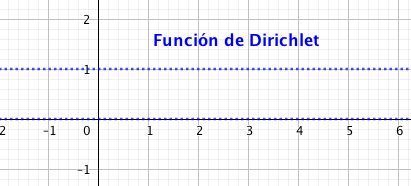
\includegraphics[width=0.4\textwidth]{imagenes/imagenes02/T02IM13.png}
			\caption{Función de Dirichlet (`discontinua' en todo su dominio).}
			\label{fig:dirichlet}
		\end{figure}
		\end{multicols}
		
		\subsection{Funciones hiperbólicas $\; \divideontimes$ }
		\label{subsec:func-hiperb}
		
		$\sinh (x)= \dfrac {e^x-e^{-x}}{2}; \qquad \cosh (x)= \dfrac {e^x+e^{-x}}{2}; \qquad \tanh (x)= \dfrac {e^x-e^{-x}}{e^x+e^{-x}}$
		
		\begin{prop} Las funciones hiperbólicas cumplen las siguientes propiedades:
		
		\begin{itemize}
			\item $\dfrac {\sinh (x)}{\cosh (x)}= \tanh (x)$
			\item $\cosh^2(x)-\sinh^2(x)=1 $
			\item $\sinh(x+y)=\sinh(x)\; \cosh (y) \; + \; \cosh(x) \; \sinh(x)$
			\item $\cosh(x+y)=\cosh(x)\; \cosh (y) \; - \; \sinh(x) \; \sinh(x)$
			%\item $(\sinh(x))'=\cosh(x); \qquad (\cosh(x))'=\sinh(x); \qquad (\tanh(x))'=\dfrac 1 {\cosh^2(x)}$
			\item El seno hiperbólico ($\sinh(x)$) y la tangente hiperbólica ($\tanh(x)$) son funciones \emph{impares}, el cosenos hiperbólico ($\cosh(x)$) es \emph{par}.
		\end{itemize}
			
		\end{prop}
		
		\begin{proof}
			La demostración es evidente a partir de las definiciones de las funciones hiperbólicas, por lo que se deja como ejercicio.
		\end{proof}

		\begin{figure}[H]
			\centering
			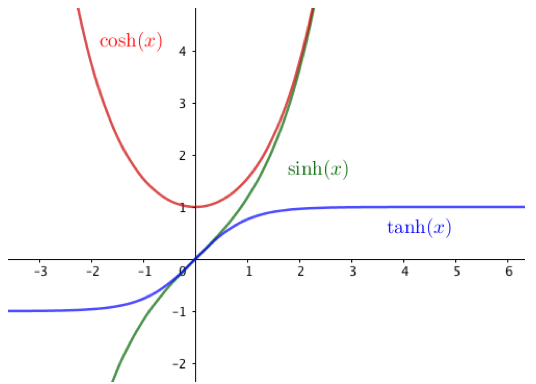
\includegraphics[width=0.5\textwidth]{imagenes/imagenes02/T02IM14.png}
			\caption{Funciones hiperbólicas.}
		\end{figure}
		
		 \small{La curva en paramétricas $x=\cosh (t);\; y=\sinh(t)$ verifica que $x^2-y^2=\cosh^2 (t)-\sinh^2(t)=1$, que corresponde a una \emph{hipérbola equilátera, por ello lo de funciones hiperbólicas. La curva en paramétricas $x=\cos (t);\; y=\sin(t)$  cumple que $x^2+y^2=1$, por ello al seno y coseno se les llaman funciones circulares.}
		
		
		\subsection{Función logí­stica  $\; \divideontimes$}
		
		Las poblaciones de seres vivos comienzan creciendo según la curva exponencial, pero con el tiempo llegan a invadir su espacio vital y su crecimiento se va amortiguando. La curva tí­pica de esta situación es la que se muestra en la siguiente figura.
		
		\begin{figure}[H]
			\centering
			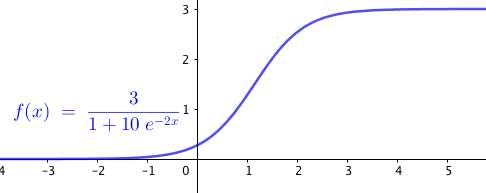
\includegraphics[width=0.4\textwidth]{imagenes/imagenes02/T02IM15.png}
			\caption{Función logí­stica.}
		\end{figure}
		
		 Función logí­stica: $f(x)=\dfrac {l}{1+ke^{-ax}}$
		
		\begin{itemize}
			\item [*] $l$ es la población lí­mite.
			\item [*] $1/(1+k)$ es la población con $x=0$
		\end{itemize}
		
		
		\section{Ejercicios}
		
		\subsection{Ejercicios Resueltos}
		
		\begin{ejre}
			De las siguientes gráficas que aparecen en la figura, ¿cuáles corresponden a una función matemática?, ¿cuáles son inyectivas?, determina el dominio y recorrido de cada una de ellas.
		\end{ejre}
		
		\begin{figure}[H]
			\centering
			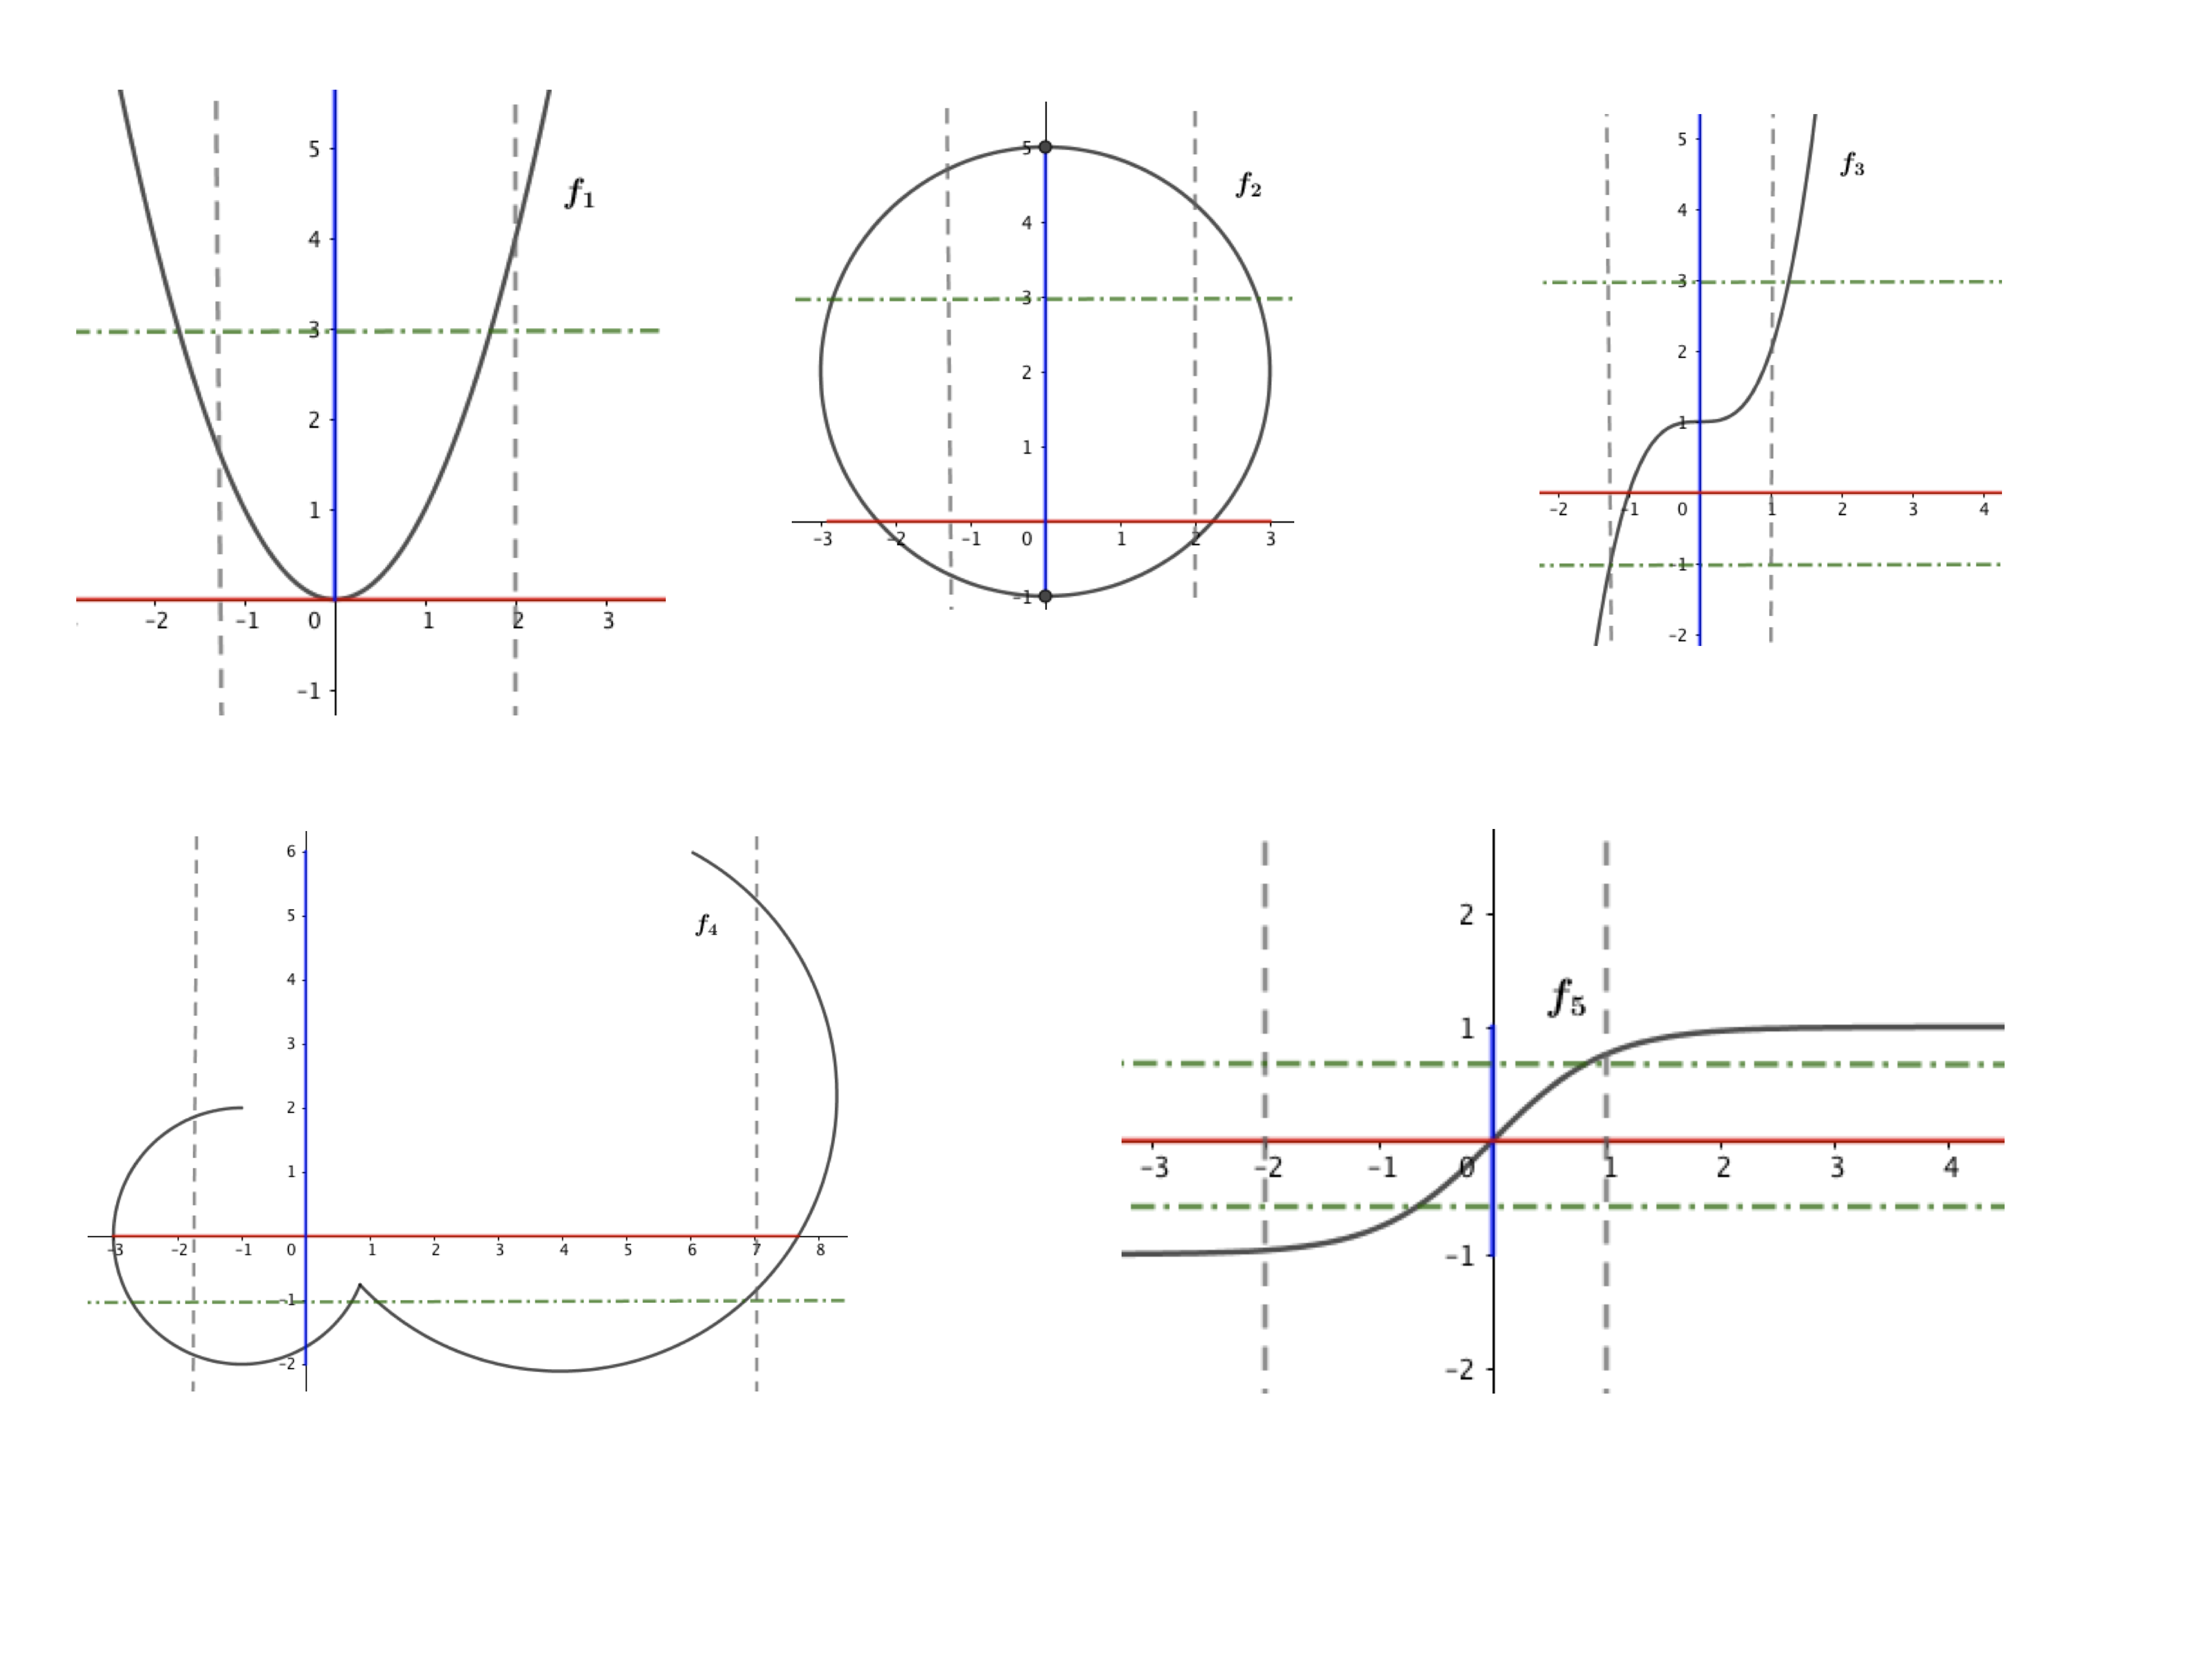
\includegraphics[width=1\textwidth]{imagenes/imagenes02/T02IM21.png}
			
		\end{figure}
		
		\begin{proofw}\renewcommand{\qedsymbol}{$\diamond$}
		En las gráficas aparece en rojo la proyección de la curva sobre $OX$, el dominio; en azul aparece la proyección de la curva sobre $OY$, el recorrido. Usamos la estrategia de la \emph{lí­nea vertical}, en gris, para saber si se trata de una verdadera función matemática y la estrategia de la \emph{lí­nea horizontal}, en verde, pasa averiguar si la función es inyectiva.
		
			 \begin{enumerate}
			 	\item [*] $f_1$: sí­ es función, no inyectiva, Dom=$\mathbb R$, Rec=$[0,\infty[$
			 	\item[*] $f_2$: no función, no inyectiva, 'dom'=$[3,4]$, 'rec'=$[-1,\infty]$
			 	\item [*] $f_3$: sí­ función, sí­ inyectica, Dom=Rec=$\mathbb R$
			 	\item [*] $f_4$: no función, no inyectiva, 'dom'=$[-3,8]$ aprox, 'rec'=$[-2,6]$ aprox.
			 	\item [*] $f_5$: sí­ función, sí­ inyectica, dom=$\mathbb R$, rec=$[-1,1]$
			 \end{enumerate}
		\end{proofw}
		
		
		
		
		\begin{ejre}
			Calcula los dominios (naturales) de las siguientes funciones:
			
		
		
		\begin{multicols}{2} 
		\begin{itemize}
		\item $f_1(x)=\dfrac 1 {1+x^2}$
		\item $f_2(x)=1+\sqrt x$
		\item $f_3(x)=\dfrac 1 {1-\sqrt x}$
		\item $f_4(x)=\sqrt{4-x^2}$
		\item  $f_5(x)=\dfrac 1 {\sqrt{4-x^2}}$
		\item $f_6(x)=\dfrac {1}{x-1} + \dfrac {1}{x+2} $
		\item $f_7(x)=\sqrt {1-x}+\sqrt {x-2}$
		\item $f_8(x)=\sqrt{1-x^2}+\sqrt{x^2-1}$
		\end{itemize}
		\end{multicols}
		

			
		\end{ejre}
		
		\begin{proofw}\renewcommand{\qedsymbol}{$\diamond$}
		
		Soluciones:
		
		\begin{itemize}
			\item [*]$f_1(x)=\dfrac 1 {1+x^2}:\qquad 1+x^2= 0 \to x=\pm \sqrt{-1} \notin \mathbb R \to \quad Dom(f_1)=\mathbb R $ 
			\item [*]$f_2(x)=1+\sqrt x: \qquad x\ge0 \to \quad Dom(f_2)=[0,\infty[=\mathbb R^+_*$
			\item [*]$f_3(x)=\dfrac 1 {1-\sqrt x}: \qquad x\ge 0,\;  $ pero $\; 1-\sqrt x \neq 0; \; \; x\neq \pm 1 \to \quad Dom(f_3)=\mathbb R^+_* \sim \{ \pm 1 \}= [0,1[ \cup ]1,\infty[$
			\item [*]$f_4(x)=\sqrt{4-x^2}: \qquad4-x^2\ge 0;\; 4-x^2=0; \; x=\pm 2$ Construimos una tabla en que estudiamos el signo de $4-x^2$.
			
		
			\begin{table}[H]
			\centering
			\begin{tabular}{|c|c|c|c|c|c|}
				\hline
				 Intervalos & $]-\infty,-2[$  & $-2$ & $]-2,2[$ & $2$ & $]2,\infty[$  \\ \hline
				 $4-x^2$& $-$ & 0 & + & 0 & $-$\\ \hline
			\end{tabular}
			\end{table}
			Luego, $Dom(f_4)=[-2,2]$
		
			\item[*]$f_5(x)=\dfrac 1 {\sqrt{4-x^2}}: \qquad $Ahora, $4-x^2>0$, no vale la opción $4-x^2=0$ porque producirí­a un cero en el denominador, por lo que, con la misma tabla anterior, $Dom(f_5)=]-2,2[$
			\item[*]$f_6(x)=\dfrac {1}{x-1} + \dfrac {1}{x+2}: \qquad D_1 \left( \frac {1}{x-1} \right)=\mathbb R \sim \{1\}; \quad D_2 \left( \frac {1}{x+2} \right)=\mathbb R \sim \{-2\} \to Dom(f_5)=D_1 \cap D_2 = \mathbb R \sim \{ -2,1 \}$
			
			
			\item[*] $f_7(x)=\sqrt{1-x}+\sqrt{x+2}: \qquad D_1: 1-x\ge 0 \to x\le 1:\; ]-\infty, 1]; \qquad D2: x-2\ge 0 \to x\ge 2: \; [2, \infty[ \quad \Rightarrow    \quad D(f_7)=D_1 \cap D_2 = \phi$
			
			\item[*]$f_8(x)=\sqrt {1-x^2}+\sqrt {^2-1}:$. Tanto $1-x^2$ como $x^2-1$ son $0$ cuando $x=\pm1$. Estudiamos los signos en la siguiente tabla:
			
			\begin{table}[H]
			\centering
			\begin{tabular}{|c|c|c|c|c|c|}
			\hline
 				Intervalos & $]-\infty,-1[$  & $-1$ & $]-1,1[$ & $1$ & $]1,\infty[$ \\ \hline
 				$1-x^2$ & $-$ & $0$ & $+$ & $0$  & $-$ \\ \hline
 				$x^2-1$ & $+$  & $0$  & $-$ & $0$  & $+$  \\ \hline
			\end{tabular}
			\end{table}
			
			Como $D_1=D(\sqrt{1-x^2})=]-\infty,-1]\cup [1,\infty]$, y $D_2=D(\sqrt{x^2-1})=[-1,1]$, entonces $Dom(f_8)=D_1 \cap D_2= \{ -1,1 \}$
			
			
		\end{itemize}
			
		\end{proofw}

		
		
		
		\begin{ejre} Dadas las funciones: $f(x)=x^2+1;\; (\forall x\ge0) \quad g(x)=\dfrac {3}{x-2}; \quad h(x)= \sqrt{x-3}$, inyectivas todas ellas en sus dominios de definición, calcula: 
		
		$g\cdot g;\quad g\circ g; \quad f\circ g; \quad g\circ f; \quad f^{-1}; \quad g^{-1}; \quad h^{-1}; \quad  f\circ f^{-1}; \quad (g \circ f)^{-1}; \quad f^{-1} \circ g^{-1} $ 
		
		Dominios y recorridos de todas ellas.
		
		\end{ejre}
		
		\begin{proofw}\renewcommand{\qedsymbol}{$\diamond$}
			
		Soluciones:
			
		\begin{itemize}
			
			
			\item [*] $g\cdot g \to g(x)\cdot g(x)= \dfrac {3}{x-2} \cdot \dfrac {3}{x-2} = \dfrac {9}{(x-2)^2}$
			\item [*] $g\circ g \to g(g(x))=g\left( \dfrac {3}{x-2} \right)=\dfrac {3}{\dfrac {3}{x-2}-2}=\dfrac {3x-6}{7-2x}$
			\item [*] $f\circ g \to f(g(x))=f \left( \dfrac {3}{x-2}  \right) = \left( \dfrac {3}{x-2}  \right)^2 +1 = \dfrac {x^4-4x+13}{x^2-4x+4}$
			
			\item [*] $ g\circ f \to g (f(x))=g(x^2+1)=\dfrac {3}{(x^2+1)-2} = \dfrac {3}{x^2-1} \quad  $ (Nótese que $g\circ f \neq f\circ g$)
			
			\item [*] $f^{-1} \to   y=x^2+1; x\leftrightarrow y: \; x=y^2+1; \; y^2=x-1; \; y=+\sqrt{x-1} \to f^{-1}(x)=+\sqrt{x-1}$
			\item [*] $g^{-1} \to  y=\dfrac {3}{x-2}; x\leftrightarrow y: \; x=\dfrac {3}{y-2}; \; x(y-2)=3; \; y=\dfrac {2x+3}{x} \to g^{-1}(x)=y=\dfrac {2x+3}{x}$
			\item [*] $h^{-1} \to y=\sqrt{x-3}; x\leftrightarrow y: \; x=\sqrt{y-3} ; \; x^2=y-3; y=x^2+3 \to h^{-1}(x)=x^2+3 $
			\item [*] $ f \left(f^{-1}(x) \right) =f (\sqrt {x-1})=(\sqrt{x-1})^2+1=x=I(x) \quad$ (Nótese que $f\circ f^{-1}=I$)
			\item [*] $ (g \circ f )^{-1} \to (g\circ f)(x)= \dfrac {3}{x^2-1}=y ; \; x\leftrightarrow y: \; \dfrac {3}{y^2-1}=x; \; y^2=\dfrac {3+x}{x}; \; y= \sqrt {\dfrac {3+x}{x}} \to  (g \circ f )^{-1}(x)=\sqrt {\dfrac {3+x}{x}}$
			\item [*] $f^{-1} \circ g^{-1} \to f^{-1} \left( g^{-1}  \right)(x)= f^{-1} \left( \dfrac {2x+3}{x} \right) = \sqrt{\left( \dfrac {2x+3}{x} \right)-1}= \sqrt{\dfrac {x+3}{x}} \to$
			
			 	$\left( f^{-1} \circ g^{-1} \right)(x)=\sqrt{\dfrac {x+3}{x}}\quad $ ( Nótese $\;(g \circ f )^{-1} =  f^{-1} \circ g^{-1} \; $ )
			 	\item [*] $Dom(f)=\mathbb R^+; \quad Rec(f)=Dom(f^{-1})=[1, \infty[; \quad Dom(g)=\mathbb R \sim \{2\}; \quad Rec(g)=Dom(g^{-1})=\mathbb R \sim \{0\}; \quad Dom(h)=[3,\infty[; \quad Rec(h)=Dom(h^{-1})=\mathbb R^+ \; $(por la zona de inyectividad de $h(x)=+\sqrt{x-3}$)
		\end{itemize}
			
		\end{proofw}
		
		
		
		\begin{ejre}
		Calcula la inversa de las funciones: $\quad f(x)=\arcsin (x^2-1); \qquad  g(x)=\ln (x^2+1)$
		\end{ejre}
		
		\begin{proofw}\renewcommand{\qedsymbol}{$\diamond$}
			
		Soluciones:
			
		\begin{itemize}
		\item[*] $y=\arcsin (x^2-1): \; x\leftrightarrow y: \; x=\arcsin (y^2-1); \; \sin x= \sin [\arcsin (y^2-1)]=y^2-1; \; y^2=\sin x +1; \; y=\sqrt{\sin x + 1} \; \to \; f^{-1}(x)=\sqrt{\sin x + 1}$	
		
		\item[*] $y=\ln (x^2+1): \; x\leftrightarrow y: \; x=\ln(y^2+1); \; e^x=e^{\ln (y^2+1)}=y^2+1; \; y^2=e^x-1; \; y=\sqrt{e^x-1} \; \to \; g^{-1}(x)= \sqrt{e^x-1}$
		\end{itemize}

		\end{proofw}
		
		
		
		
		
		\begin{ejre} Define como función a trozos: 
		\label{ejre:rompe-trozos}
			
			\begin{multicols}{2} 
			\begin{itemize}
			\item $f_1(x)=|4-x|$
			\item $f_2(x)=|-x^2-2x+3|$
			\item $f_3(x)=|\ln x|$
			\item $f_4(x)=|x|+x$
			\item $f_5(x)=|x+1|-|x-3|$
			\item $f_6(x)=|2x-4|-2|x-1|$
			\item $f_7(x)=\left| \dfrac {x^2-4}{x+1} \right|$
			\item $f_8(x)=\dfrac {|x+3|}{1+|x|}$
			\end{itemize}
			\end{multicols}
			\end{ejre}
		
		\begin{proofw}\renewcommand{\qedsymbol}{$\diamond$}
		
		Soluciones:
		
		
		\begin{itemize}
			\item [*] $f_1(x)=|4-x| \to 4-x=0;\; x=4$
			
			\begin{multicols}{2} 
			
			\begin{table}[H]
			\centering
			\begin{tabular}{|c|c|c|c|}
			\hline
			Intervalos & $]-\infty,4[$ & $4$ & $]4,\infty[$ \\ \hline
			$4-x$ & $+$ & $0$ & $-$ \\ \hline
		\end{tabular}
		\end{table}
		
		\begin{equation*}
		f_1(x)=
		\begin{cases} 
		\;\;  4-x &\mbox{if } x \le 4 \\ 
		\; x-4 & \mbox{if } x >4 
		\end{cases}
		\end{equation*}
		
		\end{multicols}
		
		\item [*] $f_2(x)=|-x^2-2x+3| \to -x^2-2x+3=0; \; x=-3, x=1 $
				\begin{table}[H]
				%\centering
				\begin{tabular}{|c|c|c|c|}
				\hline
				Intervalos & $]-\infty, -3[$ & $[-3,1[$ & $[1, \infty[$ \\ \hline
				$-(x-1)(x+3)$ & $-$ &  $+$ & $-$ \\ \hline	
				\end{tabular}
				\end{table}
			
			\begin{equation*}
				f_2(x)=
				\begin{cases} 
				\;  x^2+2x-3 &\mbox{si } x \le -3 \\ 
				\; -x^2-2x+3 &\mbox{si } -3\le x \le 1 \\
				\;  x^2+2x-3 &\mbox{si } x>1
				\end{cases}
			\end{equation*}
				
			
			
		\item[*] $f_3(x)=|\ln x| \to \ln x=0; \; x=e^0=1 \qquad \ln x:[0,\infty[ \to  \mathbb R[$
		
			\begin{multicols}{2} 
			
				\begin{table}[H]
					\centering
					\begin{tabular}{|c|c|c|c|}
					\hline
					Intervalos & $]0, 1[$ & $1$ & $]1, \infty[$ \\ \hline
					$\ln x$ & $-$ &  $0$ & $+$ \\ \hline	
					\end{tabular}
				\end{table}
			
				\begin{equation*}
					f_3(x)=
					\begin{cases} 
					\;  -\ln x &\mbox{si } 0<x<1 \\ 
					\; \ln x &\mbox{si } x\ge 1 
					\end{cases}
				\end{equation*}
				
			\end{multicols}
			
		\item [*] $f_4(x)=|x|+x$
			
				\begin{equation*}
					f_4(x)=
					\begin{cases} 
					\;  -x+x\; = \; 0 &\mbox{si } x<0 \\ 
					\; x+x\; = \; 2x&\mbox{si } x\ge 0 
					\end{cases}
				\end{equation*}
		
		\item [*] $f_5(x)=|x+1|-|x-3| \to x+1=0;x=-1; \; x-3=0; x=3$
		 
			\begin{multicols}{2} 
			
				\begin{table}[H]
					\centering
					\begin{tabular}{|c|c|c|c|}
					\hline
					Intervalos & $]-\infty, -1[$ & $[-1,3]$ & $]3, \infty[$ \\ \hline
					$x+1$ & $-$ &  $+$ & $+$ \\ \hline	
					$|x+1|$ & $-x-1$ & $x+1$ & $x+1$ \\ \hline
					$x-3$ & $-$ & $-$ & $+$ \\ \hline
					$|x-3|$ & $-x+3$ & $x-3$ & $x-3$ \\ \hline
					$f_5$ & $-4$ & $2x-2$ & $4$ \\ \hline
					\end{tabular}
				\end{table}
			
				\begin{equation*}
					f_3(x)=
					\begin{cases} 
					\;  -4 x &\mbox{si } x<1 \\ 
					\; 2x+2 &\mbox{si } -º\le x \le 3 \\
					\;    4   & \mbox{si } x>3
					\end{cases}
				\end{equation*}
				
			\end{multicols}
			
		\item[*] $f_6(x)=|2x-4|-2|x-1| \to 2x-4=0; x=2; \; x-1=0; x=1$ 
		
			\begin{multicols}{2} 
			
				\begin{table}[H]
					\centering
					\begin{tabular}{|c|c|c|c|}
					\hline
					Intervalos & $]-\infty, 1[$ & $[1,2]$ & $]2, \infty[$ \\ \hline
					$2x-4$ & $-$ &  $-$ & $+$ \\ \hline	
					  $|2x-4|$ & $-2x+4$  & $-2x+4$  & $2x-4$     \\ \hline
					 $x-1$  & $-$  & $+$  & $+$   \\ \hline
					 $-2|x-1|$  & $2x-2$  & $-2x+2$  & $-2x+2$   \\ \hline
					 $f_6$  & $2$  & $-4x+6$  & $-2$   \\ \hline 
					\end{tabular}
				\end{table}
			
				\begin{equation*}
					f_6(x)=
					\begin{cases} 
					\;  2 &\mbox{si } 0<1 \\ 
					\; -4x+6 &\mbox{si } 1\le x \le 2 \\ 
					\; -2 2 &\mbox{si } x>2
					\end{cases}
				\end{equation*}
				
			\end{multicols}
		
		\item[*] $f_7(x)=\left| \dfrac {x^2-4}{x+1} \right| \to x^2-4=0; x=\pm 2; ; x+1=0; x\neq -1$ 
		
			
			    
				\begin{table}[H]
					\centering
					\begin{tabular}{|c|c|c|c|c|}
					\hline
					Intervalos & $]-\infty, -2]$ & $]-2,-1[$&$]-1,2[$ & $[2, \infty[$ \\ \hline
					$x^2-4$ & $+$ &  $-$ & $-$ & $+$\\ \hline	
					$|x^2-4|$ & $x^2-4$ &  $-x^2+4$ & $-x^2+4$ & $x^2-4$\\ \hline
					$x+1$ & $-$ &  $-$ & $+$ & $+$\\ \hline
					$x+1$ & $-x-1$ &  $-x-1$ & $x+1$ & $x+1$\\ \hline
					$f_7$ & $-\dfrac{x^2-4}{x+1}$ &  $\dfrac{x^2-4}{x+1}$ & $-\dfrac{x^2-4}{x+1}$ & $\dfrac{x^2-4}{x+1}$\\ \hline
					
					\end{tabular}
				\end{table} 
			
				\begin{equation*}
					f_7(x)=
					\begin{cases} 
					\;  -\dfrac{x^2-4}{x+1} &\mbox{si } x\le -2 \\ 
					\; \dfrac{x^2-4}{x+1} &\mbox{si } -2<x< -1 \\
					\;  -\dfrac{x^2-4}{x+1} &\mbox{si } -1<x<2 \\ 
					\; \dfrac{x^2-4}{x+1} &\mbox{si } x\ge 2
					\end{cases}
				\end{equation*}
				
			\item[*] $f_8(x)=\dfrac {|x+3|}{1+|x|} \to x+3=0; x=-3; ; x=0$
		
				\begin{multicols}{2} 
			
				\begin{table}[H]
					\centering
					\begin{tabular}{|c|c|c|c|}
					\hline
					Intervalos & $]-\infty, -3[$ & $[-3,0]$ & $]0, \infty[$ \\ \hline
					$x+3$ & $-$ &  $+$ & $+$ \\ \hline	
					$x$   &  $-$  &  $-$  &  $+$ \\ \hline
					$f_8$   &  $\dfrac {-x-3}{1-x}$  &  $\dfrac {x+3}{1-x}$  &  $\dfrac {x+3}{1+x}$ \\ \hline
					\end{tabular}
				\end{table}
			
				\begin{equation*}
					f_8(x)=
					\begin{cases} 
					\;  \dfrac {x+3}{x-1} &\mbox{si } x<-3 \\ 
					\; \dfrac {x+3}{1-x} &\mbox{si } -3\le x \le 0 \\
					\; \dfrac {x+3}{1+x} & \mbox{si } x>0 
					\end{cases}
				\end{equation*}
				
				\end{multicols}
		
		
		\end{itemize}
		
			
		\end{proofw}
		
		
		\begin{ejre}
		Estudia la paridad de las siguientes funciones:
		
		\begin{multicols}{2} 
			\begin{itemize}
			\item $f_1(x)=x^2+1$
			\item $f_2(x)=x^5-x^3-x$
			\item $f_3(x=1-\cos x$
			\item $f_4(x)=\dfrac {x^4+1}{x^3-2x}$
			\item $f_5(x)=1-\sin x$
			\item $f_6(x)=x+\cos x$
			\item $f_7(x)=\sqrt{x^4-1}$
			\item $f_8(x)=\dfrac {x}{x^3-1}$
			\item $f_9(x)=e^{|x|}$
			\item $f_{10}(x)=\dfrac {|x|}{x^2-2x}$
			\item $f_{11}(x)=\arcsin x$
			\end{itemize}
			\end{multicols}
		
		\end{ejre}
		
		\begin{proofw}\renewcommand{\qedsymbol}{$\diamond$}	

		Soluciones:
		
		\begin{itemize}
		
			\item [*] $f_1(x)=x^2+1 \to f_1(-x)=(-x)^2+1=x^2+1=f_1(x) \quad $ PAR
			\item [*]  $f_2(x)=x^5-x^3-x \to f_2(-x)=(-x)^5-(-x)^3-(-x)=-x^5+x^3+x=-f_2(x) \quad $ IMPAR
			\item [*]  $f_3(x)=1-\cos x \to f_3(-x)=1-\cos (-x)=1-\cos x=f_3(x) \quad $ PAR
			\item [*]  $f_4(x)=\dfrac {x^4+1}{x^3-2x} \to f_4(-x)=\dfrac {(-x)^4+1}{(-x)^3-2(-x)}=\dfrac {x^4+1}{-x^3+2x}=-\dfrac {x^4+1}{x^3-2x}=-f_4(x) \quad $ IMPAR 
			\item [*]  $f_5(x)=1-\sin x \to  f_5(-x)=1-\sin (-x)=f_5(x)=1+\sin x \quad $ Sin paridad
			\item [*]  $f_6(x)=x+\cos x \to f_6(-x)=-x+\cos (-x)=-x+\cos x \quad  $ Sin paridad
			\item [*]  $f_7(x)=\sqrt{x^4-1} \to f_7(-x)=\sqrt{(-x)^4-1}=\sqrt{x^4-1}=f_7(x) \quad  $ PAR
			\item [*]  $f_8(x)=\dfrac {x}{x^3-1} \to f_8(-x)=\dfrac {-x}{(-x)^3-1}=\dfrac {-x}{-x^3-1}=\dfrac {x}{x^3+1} \quad $ Sin paridad
			\item [*]  $f_9(x)=e^{|x|} \to f_9(-x)=e^{|-x|}=e^{|x|}=f_9(x) \quad $ PAR
			\item [*]  $f_{10}(x)=\dfrac {|x|}{x^2-2x} \to f_{10}(-x)=\dfrac {|-x|}{(-x)^2-2(-x)}=\dfrac {|x|}{x^2+2x} \quad $ Sin paridad
			\item [*]  $f_{11}(x)=\arcsin x \to f_{11}(-x)=\arcsin (-x)=-\arcsin x = -f_{11}(x) \quad $ IMPAR
			
		\end{itemize}

		
		\end{proofw}
		
		\begin{ejre}
		Intenta dibujar la función: 
		\begin{equation*}
		f(x)=
		\begin{cases} 
		\;\;  x &\mbox{if } x \in \mathbb{Q} \\ 
		\; 0 & \mbox{if } x \in \mathbb{R} \sim \mathbb{Q} 
		\end{cases}
		\end{equation*}
		?`Observas algo interesante?
		\end{ejre}
		
		\begin{proofw}\renewcommand{\qedsymbol}{$\diamond$}
		
		Solución: \scriptsize{Solo `continua' en cero.}
		
			\begin{figure}[H]
			\centering
			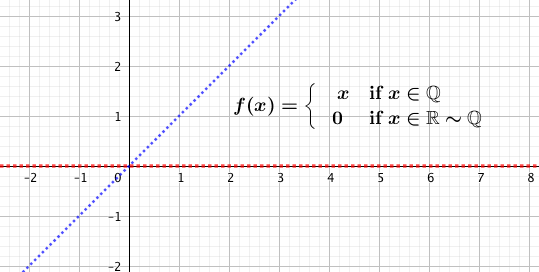
\includegraphics[width=0.5\textwidth]{imagenes/imagenes02/T02IM23.png}
			%\caption{Función solo continua en cero.}
			\end{figure}
			
		\end{proofw}
		
		\subsection{Ejercicios Propuestos}	
		
		
		\begin{enumerate}[1).-  ]
		\item A partir de la función representada en la siguiente gráfica, $f(x)$, estudia si es inyectiva, su dominio, su recorrido y, a partir de ella, representa:
		
			$f(x)+3; \quad f(x)-1; \quad f(x-2); \quad f(x+1); \quad 2f(x); \quad f(-x); \quad -f(x); \quad -f(-x)$
		
			\begin{figure}[H]
			\centering
			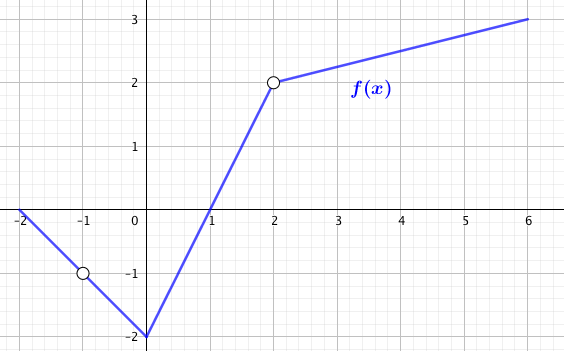
\includegraphics[width=0.6\textwidth]{imagenes/imagenes02/T02IM22.png}	
			\end{figure}
		
		
		\rightline{\textcolor{gris}{Solución:  \tiny{Sí­ inyectiva, $Dom(f)=[-2,-1[\cup ]-1,2[ \cup ]2,6]$; $\; Rec(f)=[-2,2[ \cup ]2,3]$}}}
		
		\item La \emph{función de Heaviside} es muy usada en ciencia, se define por:
		
			\begin{equation*}
			H(x)=
			\begin{cases} 
			\;\;  1 &\mbox{if } x \ge 0 \\ 
			\; 0 & \mbox{if } x<0 
			\end{cases}
			\end{equation*}
	
		Dibuja la función de Haeviside y también: $H(x)-2;\quad H(x-2); \quad -H(x-2)-2$
		
		\item Calcula el dominio de las siguientes funciones:
		
		\begin{multicols}{2} 
		\begin{enumerate}[a.]
		\item $f(x)=\ln{4-\sqrt x}$
		\item $f(x)=\dfrac 1 {\tan x}$
		\item $f(x)=\dfrac 1 {\sqrt {\tan^2 x - 1}}$
		\item $f(x)=\dfrac {2}{1-\cos x}$
		\item $f(x)=\dfrac {1}{\sin x - \frac 1 2}$
		\end{enumerate}
		\end{multicols}

		
		\rightline{\textcolor{gris}{Solución:  $D_a=[0,16[;\quad D_b=\mathbb R \sim \{ k\pi, (2k+1)	pi /2\};\; \forall k \in \mathbb Z$}}
		\rightline{\textcolor{gris}{ $D_c=[-\frac {\pi}{2}+k\pi, -\frac {\pi}{4}+k\pi[ \cup ] \frac {\pi}{4}+k\pi , \frac {\pi}{2} +k\pi  [ ; \; \forall k\in \mathbb Z$}}
		\rightline{\textcolor{gris}{ $D_d=\mathbb R \sim \{2k\pi; \; \forall k \in \mathbb Z \} \quad D_e= \mathbb R \sim \{ \frac {\pi}{6}+2k\pi, \; \frac {5\pi}{6}+2k\pi ;\;\forall k \in \mathbb Z \}$ }}
		
		
		\item Dadas las funciones: $f(x)=\sin x ; \quad g(x)=\pi x$, evalúa las expresiones siguientes:
		
		 	\begin{multicols}{3} 
			\begin{enumerate}[a.]
				\item $f(g(2))$
				\item $f(g(1/2))$
				\item $g(f(0))$
				\item $g(f(\pi /4))$
				\item $f(g(x))$
				\item $g(f(x))$
			\end{enumerate}
			\end{multicols}
			
			\rightline{\textcolor{gris}{Solución: a)$0$; b)$1$; c)$0$ }}
			\rightline{\textcolor{gris}{Solución: d)$\sqrt 2 \pi /2$;  e) $\sin \pi x$;  f) $\pi \sin x$ }}
		
		 
		 \item para los siguientes pares de funciones, calcula $f\circ f$, $g \circ f$ y los dominios de ambas composiciones.
		 
		 	\begin{multicols}{2}
		 	\begin{enumerate}[a. ]
		 		\item $f(x)=\frac 3 x \; ;\quad g(x)=x^2-1$
		 		\item $f(x)= \frac 1 x\; ; \quad g(x)=\sqrt{x+2}$
		 	\end{enumerate}	
		 	\end{multicols}
			
			\rightline{\textcolor{gris}{Solución: a) $D(f\circ g)=\mathbb R \sim \{ -1,1\}; \quad D(g\circ f)=\mathbb R \sim \{ 0\}$ }}
			\rightline{\textcolor{gris}{Solución: b) $D(f\circ g)=]-2, \infty[; \quad D(g\circ f)=]-\infty, -1/2] \cup ]0, \infty[$  }}

		 \item Determina $f\circ g$ siendo las funciones $f$ y $g$ las definidas definidas por: 
		 
		 	\begin{equation*}
			f(x)=
			\begin{cases} 
			\;\;  x+3 &\mbox{if } x<0 \\ 
			\; 2x^2+3 & \mbox{if } x\ge 0 
			\end{cases}
			\qquad g(x)=x+1
			\end{equation*}
		 
		 \item Calcula la inversa de la función $f(x)=\sqrt{\dfrac{x-1}{x+1}}$
		
		 \rightline{\textcolor{gris}{Solución: $y=\frac {x^2+1}{x^2-1} $}}

		

		
		\item Si $f(2^x)=x^2$, calcula $f(16)$
		 
		\rightline{\textcolor{gris}{Solución: 16}}
		
		
		
		\item Si $f(2x-1)=x$, calcula $f(2)$
		 
		\rightline{\textcolor{gris}{Solución: $3/2$}}
		
		
		
		\item Si $f(x+4)=2x+3$, calcula $f(f(f(f(x))))$
		 
		\rightline{\textcolor{gris}{Solución: $3x-155$}}
		
		
		
		\item Si $f(x)=\dfrac {x}{x-1}, \; x\neq 1$, calcula $(f\circ f \circ \cdots \circ f)_{9\mbox{ veces }}(x)$
		 
		\rightline{\textcolor{gris}{Solución: f(x)}}
		
		
		
		\item Si $f(x)=\dfrac {x+1}{x-1}$, calcula $f(f(f(f(2020))))$
		 
		\rightline{\textcolor{gris}{Solución: 2020 }}
		
		\item Si $f(f(f(f(x))))=16x+15$, calcula $f(7)$
		 
		\rightline{\textcolor{gris}{Solución: ayuda, considera $f(x)=ax+b$}}
		
		\item Sea $f(x)=x^3+3$, $g(f(x))=x,\; \forall x$, calcula $g(30)$
		 
		\rightline{\textcolor{gris}{Solución: 3}}
		
		\item $\divideontimes$. Sea $f(x)$ una función real de variable real tal que $f(x-5)=f(x+5)$ y se sabe que tiene 5 raí­ces reales distintas \scriptsize{(raí­z de $f(x)$ es cada una de las soluciones de la ecuación $f(x)=0$)} \normalsize{Calcula la suma de todas ellas.}
		 
		\rightline{\textcolor{gris}{Solución:25 }}
		
		
			
		\end{enumerate}
		

			




\chapter{Límites y Continuidad}	
\label{Límites y Continuidad}
	\section{Introducción}
	
		

	En este tema vamos a estudiar, con algún detalle, el importante concepto teórico que es el de \emph{continuidad}. Para motivar la definición que vamos a dar de continuidad, consideremos una ley física de la forma $T = f (l )$, que relaciona los valores de una variable independiente $l$ (la longitud de la cuerda de un péndulo) con otra variable dependiente $T$ (el periodo o tiempo en dar una oscilación completa).Si queremos usar dicha ley, hemos de medir un valor $l_0$ de la variable $l$ , y es inevitable que al hacerlo cometamos algún error el cual, naturalmente, influye en el correspondiente valor de $T$, que ya no será exactamente igual a $T_0 = f(l_0)$. Surge así la pregunta natural: ?`de qué forma el error en la medida de $l$ afecta al valor resultante de $T$ ? Es claro que si para valores de $l$ muy próximos a $l_0$ obtengo valores de $T$ muy diferentes entre sí, la ley `$f$' que relaciona $l$ con $T$ no tendrá ninguna utilidad práctica.

	Puesto que los errores de medida son inevitables, no es razonable tratar de obtener el verdadero valor $T_0$. Lo que sí puede hacerse es fijar una cota de error admisible para $T$ (la cual dependerá de cada situación concreta), llamemos $\varepsilon$ (épsilon) a dicha cota, $\varepsilon > 0$, y tratar de obtener otra cota de error $\delta$ (delta) $\delta > 0$, de tal forma que siempre que midamos $l_0$ con un error menor que $\delta$ tengamos la seguridad de que el valor resultante para $T$ se diferencie de $T_0$ en menos que $\varepsilon$. Esto es, $|f(l )-f(l_0)|=|T-T_0| < \varepsilon$ siempre que $|l-l_0| < \delta$. Cuando esto efectivamente pueda hacerse para cualquier cota de error $\varepsilon > 0$ diremos que la ley `$f$'  es continua en $l_0$.

	Cabe esperar que la cota de error $\delta$ dependa del $\varepsilon$ fijado en cada caso. Intuitivamente, cuanto más pequeño sea el error permitido en los datos finales, tanto mejor tendremos que medir la variable independiente. En general, la precisión $\delta$  con la que debemos medir $l_0$ para obtener un error final menor que $\varepsilon$, depende no solamente del valor fijado de $\varepsilon$ sino también del valor de $l_0$. Esto es fácil de entender, no es lo mismo medir una longitud de varios metros que otra de unos pocos milímetros, la precisión de nuestra medida debe ser mejor en este último caso.

\textcolor{gris}{La fórmula física que describe el periodo del péndulo físico es $T=k\; \sqrt{l}\; \quad k=\frac {1}{2\pi \sqrt{g} }=cte; (g text{ es la aceleración de la gravedad})$}

	Las ideas anteriores conducen, de forma natural, a la definición matemática de continuidad. En todo lo que sigue, la letra $A$ representará un conjunto no vacío de números reales. En la práctica $A$ será siempre un intervalo o una unión de intervalos. Recuérdese que la notación $f : A \to \mathbb R$ quiere decir que $f$ es una función real cuyo dominio es $A$. Es muy importante advertir que $A$ no tiene por qué coincidir con el dominio natural de la función. Esto es así porque con frecuencia estamos interesados en estudiar propiedades de una función en una parte de su dominio natural. Además, la continuidad de $f$ depende tanto de la `regla que la define' como del conjunto en donde estamos trabajando. 
	
	Toda la idea de función continua se basa en el concepto fundamental de \emph{límite}, que desarrollamos a continuación.
	
	
	\section{Límite de una función en un punto}
	
	Empezaremos con una definición \emph{informal} de límite y daremos, más tarde, la definición formal.
	
	\begin{defi}
	
	Sea $f(x)$ una función definida en un intervalo abierto alrededor de $x_0$, excepto, posiblemente, en el propio $x_0$. Si ocurre que $f(x)$ se aproxima tanto como queramos a $L$ a medida que estemos lo suficientemente cerca de $x_0$, diremos que \textit{el límite de $f(x)$ es $L$ cuando $x$ se acerca, o tiende, a $x_0$} y lo denotaremos así:
	
	\begin{equation}
		\underset { x\rightarrow x_0 }{ lim } {f(x)}=L
	\end{equation}
		
	\end{defi}

	
	Con esta definición \emph{informal} queremos decir que $f(x)$ se acerca al número $L$ tanto como queramos, sin más que tomar valores $x$ lo suficientemente cerca de $x_0$ (por cualquiera de sus lados). Veamos un ejemplo:
	
	\begin{ejem}
		Estudia $\quad \underset { x\rightarrow 1 }{ lim } \; {\dfrac {x^2-1}{x-1}}$
	\end{ejem}
	
	Para ello vamos a construir dos sucesiones que se vayan aproximando a $1$ por cada lado, con números mayores que $1$ ($1^+$, nos acercamos a $1$ por su derecha) y con números menores que $1$ ($1^-$, nos acercamos a $1$ por su izquierda) y observemos que hace la función a medida que nos acercamos más y más a $1$.
	
	
	\begin{table}[H]
	\centering
	\begin{tabular}{l|lll|l}
	\multicolumn{1}{c|}x{} & \multicolumn{1}{c}f(x){} & \multicolumn{1}{c}{} & \multicolumn{1}{c|}x{} &  f(x)
	
	\\ \cline{1-2} \cline{4-5} 
       
         $0.9$&$1.9$&    $\qquad \qquad$      &$1.1$&$2.1$   \\
         $0.99$&$1.99$&        &$1.01$&$2.01$    \\
         $0.999$&$1.999$&      &$1.01$&$2.01$      \\
         $...$&$...$&          &$...$&  $...$      \\
         $\to 1^-$&$\to 2$&    &$\to 1^+$&$\to 2$   \\
                     
	\end{tabular}
	\end{table}
	
	Decimos que $\quad \underset { x\rightarrow 1 }{ lim } \; {\dfrac {x^2-1}{x-1}} = 2$ queriendo indicar que $f(x)$ se aproxima a $2$ cada vez que $x$ se acerca a $1$ y esto es independiente del valor que tenga $f(1)$, que en este caso no existe.
	
	En algunas ocasiones se puede calcular  $\quad \underset { x\rightarrow x_0 }{ lim } {f(x)}$ calculando $f(x_0)$ y esto ocurre cuando no se produce una \emph{indeterminación}, algo que no sabemos calcular. Ya veremos que son y como reaccionar ante una de estas  \emph{indeterminaciones}. Por ejemplo, en el caso anterior, si queremos calcular  $\quad \underset { x\rightarrow 3 }{ lim } \; {\dfrac {x^2-1}{x-1}}$, basta con calcular $f(3)=4$, ya que en este caso, el cálculo de $f(3)$ no nos ha provocado ninguna indeterminación, si hubiésemos aplicado el método anterior de ir aproximándonos a $3$ por la izquierda y la derecha hubiésemos obtenido que el límite era $f(3)=4$. No ocurría lo mismo en el caso anterior, si deseamos calcular $f(1)$ obtendremos $\frac 0 0$, cuyo valor nos resulta desconocido (\emph{indeterminación}).
	
	
	\subsection{Límites laterales}
	
	
	Sea $x_0 \in \mathbb R$, para estudiar el $ \underset { x\rightarrow x_0}{ lim } \; {f(x)}$, si se obtiene límite $\infty$ o bien $x_0$ es el nexo de una función definida a trozos (punto en el que cambia la característica o fórmula de la función a la izquierda o derecha de $x_0$) estudiaremos los límites laterales, y además,
	
	\begin{equation}	
	\exists \underset {x\to x_0}{lim}{f(x)} \leftrightarrow \exists \underset {x\to x_0^+}{lim}{f(x)} \; \wedge \;  \exists \underset {x\to x_0^-}{lim}{f(x)} \; \mbox { y } \;   \underset {x\to x_0^+}{lim}{f(x)}= \underset {x\to x_0^-}{lim}{f(x)}
	\end{equation}
	
	 \emph{`El límite, si existe, es único'}
	
	\subsection{Límites infinitos}
	
	Continuamos con una definición, también informal de momento, de lo que entendemos por límite infinito de una función en un punto.
	
	\begin{defi}
	
	Sea $f(x)$ una función definida en un intervalo abierto alrededor de $x_0$, excepto, posiblemente, en el propio $x_0$. Si ocurre que $f(x)$ toma cada vez valores más y más grandes  a medida que estemos lo suficientemente cerca de $x_0$, diremos que \textit{el límite de $f(x)$ cuando $x$ se acerca, o tiende, a $x_0$} es $+\infty$ y lo denotaremos así:
	
	\begin{equation}
		\underset { x\rightarrow x_0 }{ lim } {f(x)}=+\infty
	\end{equation}
	
	Análogamente, diremos que $f(x)$ una función definida en un intervalo abierto alrededor de $x_0$, excepto, posiblemente, en el propio $x_0$, si ocurre que $f(x)$ toma cada vez valores más y más grandes pero negativos a medida que estemos lo suficientemente cerca de $x_0$, diremos que \textit{el límite de $f(x)$  cuando $x$ se acerca, o tiende, a $x_0$} es $-\infty$ y lo denotaremos así:
	
	\begin{equation}
		\underset { x\rightarrow x_0 }{ lim } {f(x)}=-\infty
	\end{equation}
		
	\end{defi}
	
	\begin{ejer}
		Estudia $\quad \underset { x\rightarrow 1 }{ lim } \; {\dfrac {1}{x-1}}$
	\end{ejer}

	
	Para ello vamos a construir dos sucesiones que se vayan aproximando a $1$ por cada lado, con números mayores que $1$ ($1^+$) y con números menores que $1$ ($1^-$) y observemos que hace la función a medida que nos acercamos más y más a $1$.
	
	
	\begin{table}[H]
	\centering
	\begin{tabular}{l|lll|l}
	\multicolumn{1}{c|}x{} & \multicolumn{1}{c}f(x){} & \multicolumn{1}{c}{} & \multicolumn{1}{c|}x{} &  f(x)
	
	\\ \cline{1-2} \cline{4-5} 
       
         $0.9$&$-10$&    $\qquad \qquad$      &$1.1$&$10$   \\
         $0.99$&$-100$&        &$1.01$&$100$    \\
         $0.999$&$-1000$&      &$1.01$&$1000$      \\
         $...$&$...$&          &$...$&  $...$      \\
         $\to 1^-$&$\to -\infty $&    &$\to 1^+$&$\to \infty$   \\
                     
	\end{tabular}
	\end{table}
	
	Decimos que $\quad \underset { x\rightarrow 1^- }{ lim } \; {\dfrac {1}{x-1}} = -\infty$ queriendo indicar que $f(x)$ se aproxima a $-\infty$ cada vez que $x$ se acerca a $1^-$ y esto es independiente del valor que tenga $f(1)$, que en este caso no existe. Análogamente, decimos que $\quad \underset { x\rightarrow 1^+ }{ lim } \; {\dfrac {1}{x-1}} = +\infty$ queriendo indicar que $f(x)$ se aproxima a $+\infty$ cada vez que $x$ se acerca a $1^+$ . Abusando del lenguaje, podemos decir que $\quad \underset { x\rightarrow 1 }{ lim } \; {\dfrac {1}{x-1}} = \infty$, sin especificar el signo con el cual la función diverge a $\infty$. Si por ambos lados ocurre que el límite diverge a $+\infty$ o $-\infty$ sí podemos precisar que $\quad \underset { x\rightarrow x_0}{ lim } \; {f(x)} = +\infty \quad $ ó $\quad \underset { x\rightarrow x_0}{ lim } \; {f(x)} = -\infty$

	

	
	\section{Límites en el infinito}
	
	 \begin{defi}.
	 
	 Decimos que $\underset {x \to \pm \infty}{lim}{f(x)}= L$ si para toda sucesión de originales $x$ que diverjan a $\infty$, los valores que va tomando $f(x)$ se aproximan más y más a $L$
	 
	 Decimos que $\underset {x \to \pm \infty}{lim}{f(x)}= \pm \infty$ si para toda sucesión de originales $x$ que diverjan a $\infty$, los valores que va tomando $f(x)$ se aproximan más y más a $\pm \infty$
	 
	 \begin{equation}
	 	\underset {x\to \pm \infty}{lim}{f(x)}=L \quad \mbox{o} \quad \underset {x\to \pm \infty}{lim}{f(x)}=\pm \infty
	 \end{equation}

	 	
	 \end{defi}

	\vspace{2mm} Los límites en el infinito requieren un tratamiento distinto a los límites de una función en un punto:
	
	\begin{itemize}
		\item [*] Las funciones polinómicas tienen límite infinito en el infinito, el signo lo determina el signo del coeficiente del término dominante del polinomio.
		\item [*] Para funciones racionales (cocientes de polinomios), si el grado del numerador es superior al del denominador, el límite es infinito. Si el denominador es el que posee grado mayor al denominador, el límite es cero. En el caso en que numerador y denominador sean del mismo grado, el límite en el infinito es el cociente de los coeficientes de los términos dominantes (del mismo grado) de numerador y denominador.
		\item ORDEN DE INFINITOS: 
		
		\hspace{10mm} $a>1;\; n>0; \; b>1:\; \mbox{ si } x \to \infty: \quad a^x>>x^x>>log_bx$
		\item Para calcular $\underset {x \to -\infty}{lim}{f(x)} = [\mbox{cambio } x=-t] =\underset {t \to +\infty}{lim}{f(-t)}$
	\end{itemize}
	
	 NOTA: cuando al calcular un límite la función se acerca a un número real $L$, decimos que $f(x)$ \emph{converge} a $L$. Si la función se aleja al $\infty$, decimos que $f(x)$ \emph{diverge} a $\infty$.

	
	 Veamos algunos ejemplos:
	
	\begin{ejem}Ejemplos de límites en el $\infty$.
	\begin{multicols}{2}
	\begin{itemize}
		\item $\underset {x \to \infty }{lim}{3x^2-4x^5+5x-2}=-\infty  $
		\item $\underset {x \to \infty }{lim}{\frac {3x^2-1}{3-2x^2}}=\frac {3}{-2}=-\frac 3 2  $
		\item $\underset {x \to \infty }{lim}{\frac {3x^2-1}{3x^4-2x^2}}=0$
		\item $\underset {x \to \infty }{lim}{\frac {3x^2-1}{3-2x}}=-\infty$ (denominador negativo)
		\item $\underset {x \to \infty }{lim}{x^3-e^x}=-\infty$ ($e^x>>x^3$, para $x>>1$)
	\end{itemize}	
	\end{multicols}
	\end{ejem}
	
	

	 
	\section{Límites a partir de gráficas}
	
		\begin{ejem} Calcula los límites de $f(x)$ cuando $x$ tiende a $0$, $2$ y $4$ a partir de la siguiente gráfica.
		
	    \begin{multicols}{2}
	    
		\begin{figure}[H]
			\centering
			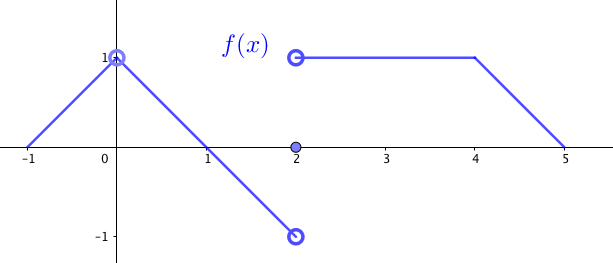
\includegraphics[width=0.5
			\textwidth]{imagenes/imagenes03/T03IM01.png}
		\end{figure}
		
		\begin{itemize}
			\item $\underset { x\rightarrow 0}{ lim } {f(x)}=1; \qquad \nexists f(1)$
			\item $\nexists \underset { x\rightarrow 2}{ lim } {f(x)}\text{:} \;  \underset { x\rightarrow 2-}{ lim } {f(x)}=-1; $
			
			$  \underset { x\rightarrow 2^+}{ lim } {f(x)}=1; \qquad  f(2)=0$
			\item $\underset { x\rightarrow 4}{ lim } {f(x)}=1; \qquad f(4)=1$
		\end{itemize}
	
	   \end{multicols}
	   
	   \end{ejem}
	   
	   \begin{ejem} Calcula los límites de $f(x)$ a partir de la siguiente gráfica, en los puntos $\{-4, -2, 0, 1, 3, 5, 7, 8, 10 \}$ y en $\pm \infty$.
	   
	   \begin{figure}[H]
			\centering
			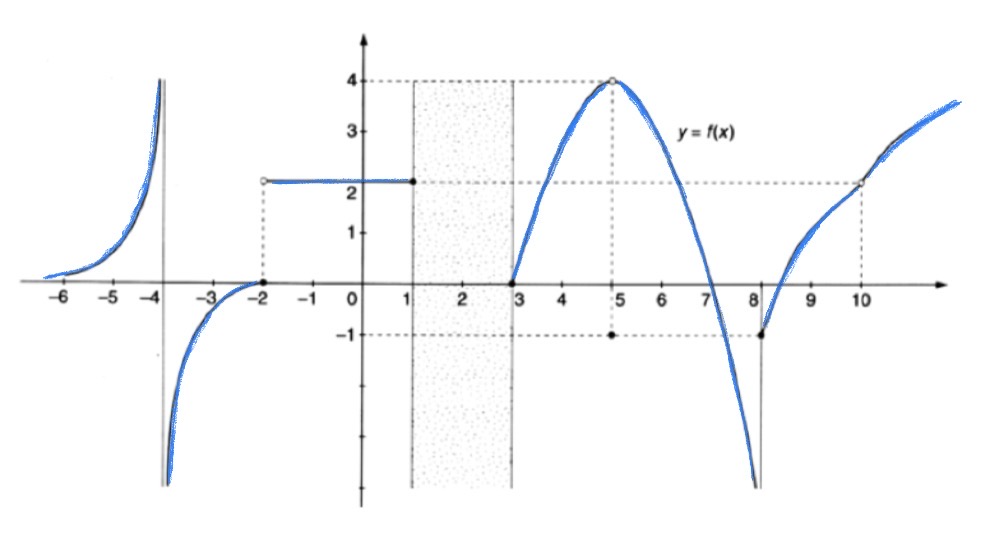
\includegraphics[width=.95
			\textwidth]{imagenes/imagenes03/T03IM02.png}
		\end{figure}
	   	
	   	\begin{itemize}
	   		\item $\underset {x \to -4^-} {lim} {f(x)}= +\infty; \quad \underset {x \to -4^+} {lim} {f(x)}=-\infty; \quad \nexists f(-4) $
	   		\item $\underset {x\to -2^-} {lim} {f(x)}=0; \quad \underset {x \to -2^+} {lim} {f(x)}=2; \quad f(2)=0$
	   		\item $\underset {x \to 0} {lim} {f(x)}=2; \quad f(0)=2$
	   		\item $\underset {x \to 1^- } {lim} {f(x)}=2; \quad \nexists \underset {x \to 1^+} {lim} {f(x)}; \quad f(1)=2$
	   		\item $\nexists \underset {x \to 3^-} {lim} {f(x)}; \quad \underset {x \to 3^+ } {lim} {f(x)}= 0; \quad f(3)=0 $
	   		\item $\underset {x \to 5} {lim} {f(x)}=4; \quad f(5)=-1$
	   		\item $\underset {x \to 7} {lim} {f(x)}=0; \quad f(7)=0$
	   		\item $\underset {x \to 8^-} {lim} {f(x)}=-\infty; \quad \underset {x \to 8^+} {lim} {f(x)}=-1; \quad f(8)=-1$
	   		\item $\underset {x \to 10} {lim} {f(x)}=2; \quad \nexists f(10)$
	   		\item $\underset {x \to -\infty}{lim}{f(x)}=0; \quad \underset {x \to \infty}{lim}{f(x)}=+\infty$
	   	\end{itemize}
	   	
	   \end{ejem}

	   \begin{ejem} Funciones exponencial y logarítmica.
	   	
	   	\begin{multicols}{2}
	    
			\begin{figure}[H]
			\centering
			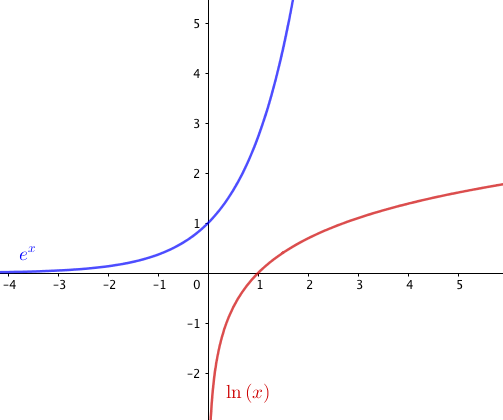
\includegraphics[width=0.3
			\textwidth]{imagenes/imagenes03/T03IM03.png}
			\end{figure}
		
			\begin{itemize}
			\item $\underset {x \to -\infty}{lim}{e^x}=0$
			\item $\underset {x \to +\infty}{lim}{e^x}=+\infty$
			\item $\underset {x \to 0^+}{lim}{\ln x}=-\infty$
			\item $\underset {x \to +\infty}{lim}{\ln x}=+\infty$
			\end{itemize}
	
	   \end{multicols}
	   	
	   \end{ejem}



		\begin{ejem}.
	   	
	   	\begin{multicols}{2}
	    
			\begin{figure}[H]
			\centering
			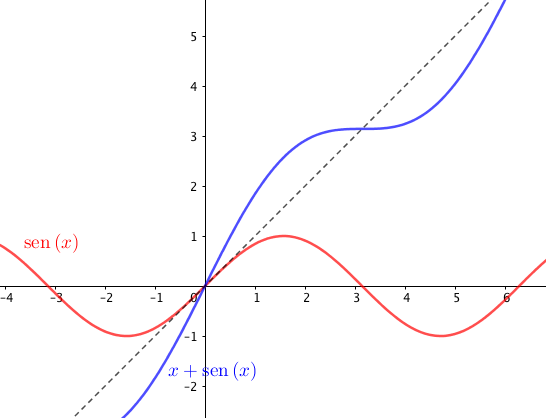
\includegraphics[width=0.4
			\textwidth]{imagenes/imagenes03/T03IM04.png}
			\end{figure}
		
			\begin{itemize}
			\item $\nexists \underset {x \to -\infty}{lim}{\sin x}$
			\item $\nexists \underset {x \to +\infty}{lim}{\sin x}$
			\item $\underset {x \to -\infty}{lim}{(x+\sin x)}=-\infty$
			\item $\underset {x \to +\infty}{lim}{(x-\sin x)}=+\infty$
			\end{itemize}
	
	   \end{multicols}
	   	
	   \end{ejem}.
	   
	   
	   \begin{ejem}.
	   	
	   	\begin{figure}[H]
			\centering
			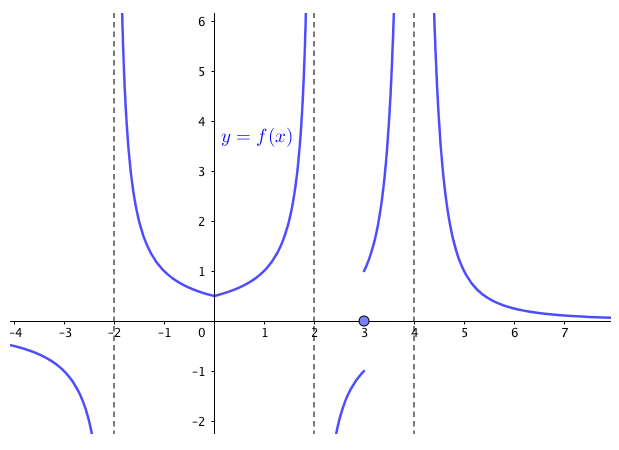
\includegraphics[width=0.8
			\textwidth]{imagenes/imagenes03/T03IM05.png}
			\end{figure}
		
	   	 	\begin{multicols}{2}
	   	 		\begin{itemize}
	   	 			\item $\underset {x\to -\infty}{lim}{f(x)}=0  $
	   	 			\item $\underset {x\to -2^{\mp}}{lim}{f(x)}=\mp \infty  $
	   	 			\item $\underset {x\to 0}{lim}{f(x)}=1/2=f(0)  $
	   	 			\item $\underset {x\to 2^{\mp}}{lim}{f(x)}=\pm \infty  $
	   	 			\item $\underset {x \to 3^{\mp}}{lim}{f(x)}=\mp 1; ;\ f(3)=0  $
	   	 			\item $\underset {x\to 4^{\mp}}{lim}{f(x)}=+\infty  $
	   	 			\item $\underset {x\to +\infty}{lim}{f(x)}=0  $
	   	 		\end{itemize}	
	   	 	\end{multicols}

	   \end{ejem}
	   
	   \section{Álgebra de límites. Indeterminaciones}
	   
		El siguiente teorema (que daremos sin demostración) nos enseña como calcular límites en un punto de funciones que son combinaciones aritméticas de otras funciones cuyos límites, en esos puntos, conocemos (siempre que no lleguemos a una \emph{indeterminación}).
		
		\begin{teor}{Álgebra de límites. }
		
		Sean $L, M, x_0, k \in \mathbb R \quad $, con $\quad \underset {x \to x_0}{lim}{f(x)}=L; \; \underset {x \to x_0}{lim}{g(x)}=M \quad \Rightarrow$
		
		\begin{itemize}
			\item [*] `El límite de la suma (de dos funciones) es la suma de los límites'.
			
				$\underset {x\to x_0}{lim}{(f(x)+g(x))}=\underset {x\to x_0}{lim}{f(x)}+\underset {x\to x_0}{lim}{g(x)}=L+M$
			\item [*]`El límite de la resta es la resta de los límites'.
			
				$\underset {x\to x_0}{lim}{(f(x)-g(x))}=\underset {x\to x_0}{lim}{f(x)}-\underset {x\to x_0}{lim}{g(x)}=L-M$
			\item [*]`El límite del producto es el producto de los límites'.
						
				$\underset {x\to x_0}{lim}{(f(x)\cdot g(x))}=\underset {x\to x_0}{lim}{f(x)} \cdot \underset {x\to x_0}{lim}{g(x)}=L\cdot M$

			\item [*]`El límite del producto de una constante por una función es el producto de la constante por el límite de la función'.
						
				$\underset {x\to x_0}{lim}{(k\cdot f(x))}=k\cdot \underset {x\to x_0}{lim}{f(x)}=k\cdot L$
				
			\item [*]`El límite del cociente es el cociente de los límites, siempre que el denominador no sea cero'.
						
				$\underset {x\to x_0}{lim}{\dfrac {f(x)} {g(x)}}= \dfrac {\underset {x\to x_0}{lim}{f(x)}} {\underset {x\to x_0}{lim}{g(x)}}=\dfrac L M; \quad M\neq 0$
				
				\item [*]`El límite de la potencia es la potencia de los límites' (siempre que no se produzca indeterminación).
						
				$\underset {x\to x_0}  {lim} { \left( f(x) ^ {g(x)} \right) } = \underset {x \to x_0}{lim}{f(x)} ^ { \underset {x \to x_0}{lim}{g(x)}  } = L^M$
				
				\end{itemize}
				
				Nota: todas estas propiedades también se cumplen cuando $x\to \pm\infty$
			
		\end{teor}
		
			\textbf{Indeterminaciones:} Llamamos \emph{indeterminación} a una expresión algebraica cuyo resultado nos es desconocido, surgen al aplicar el álgebra de límites  y obtener uno de estos $7$ resultados (\textit{indeterminaciones}):
				
				\begin{equation}
					\infty - \infty; \quad \infty \cdot 0; \quad \frac 0 0; \quad \frac {\infty}{\infty}; \quad 0^0; \quad \infty ^0; \quad 1^{\infty}
						\label{indeterminaciones}
				\end{equation}
				
				Para resolver estas indeterminaciones desarrollaremos estrategias que nos permitirán encontrar su valor sin aplicar el álgebra de límites:
				 
				\begin{itemize}
					\item En cocientes de polinomios factorizaremos por Ruffini.
					\item Si aparecen raíces cuadradas usaremos el método del conjugado
					\item En las indeterminaciones con potencias tomaremos logaritmos, pues se cumple que: $\ln {\underset {x \to x_0}{ lim}{f(x)} }= \underset {x \to x_0}{lim}{\ln f(x)}$
				\end{itemize}
				
		
		 
		 ATENCIÓN: no son indeterminaciones:
		
		
			\begin{figure}[H]
			\centering
			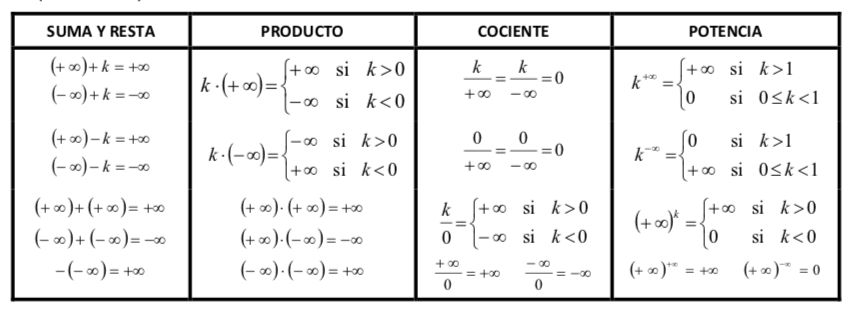
\includegraphics[width=1
			\textwidth]{imagenes/imagenes03/T03IM06.png}
			\end{figure}
	
	
	
	\section[Criterio del Sandwich y teorema de la conservación del signo $\; \divideontimes$]{Criterio del Sandwich y teorema de la conservación del signo $\; \divideontimes$}
	\sectionmark{Ths. Sandwid y conservación signo}
	
	\vspace{2mm}\begin{teor} {Teorema (criterio) del Sandwich.}
	\label{teor:Sandwich}
	Supongamos que $g(x)\le f(x) \le h(x)$ para todo $x$ en algún intervalo abierto que contenga a $x_0$, excepto posiblemente en el propio $x_0$, supongamos también que $\underset {x\to x_0}{lim}{g(x)}=\underset {x\to x_0}{lim}{h(x)}=L$, entonces: $\underset {x\to x_0}{lim}{f(x)}=L$
		
	\end{teor}
	
	\begin{ejem}.
	\label{ejem:sinx/x}
		
		\begin{multicols}{2}
			\begin{figure}[H]
			\centering
			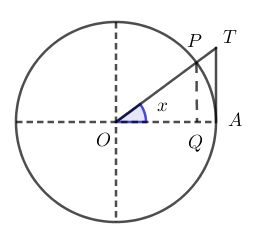
\includegraphics[width=0.4
			\textwidth]{imagenes/imagenes03/T03IM07.png}
		\end{figure}
		
		En una circunferencia de radio $1$ tomamos un ángulo $\widehat { AOP } $ de $x$ radianes. $\overline { PQ } =\sin  x; \quad \overline {TA}=\tan x; \quad $ arco $\; \widehat { PA } =x$
		
		Como $\overline {PQ}<\widehat{PA}<\overline{TA} \to \sin x < x < \tan x$
			
		Dividiendo por $\sin x \quad : 1< \dfrac {x}{\sin x}< \dfrac {1} {\cos x} \to 1> \dfrac {\sin x}{x} > \cos x$
		
		Tomando límites cuando $x\to 0: \quad 1 \ge \dfrac {\sin x}{x} \ge \cancelto {1}{\cos x} $
		
		Luego:  $\quad \underset {x\to 0}{lim}\; {\dfrac {\sin x}{x}}=1$
		\end{multicols}

		
	\end{ejem}
	
	\begin{teor}
	
	
	Si $f(x) \le g(x)$  para todo $x$ en algún intervalo abierto que contenga a $x_0$, excepto posiblemente en el propio $x_0$, y existen los límites de $f(x)$ y de $g(x)$ cuando $x\to x_0$, entonces: $\underset {x\to x_0}{lim}{f(x)} \le \underset {x\to x_0}{lim}{g(x)}$
		
	\end{teor}
	
	\begin{lema}Teorema de conservación del signo.
	\label{teor:conserva-signo}
	
	Sea $f:[a,b]\to \mathbb R$, continua en $x_o \in ]a,b[ \; \Rightarrow \mbox{ si } f(x_0)\neq 0 \to \exists \; E_{\delta}(x_0)=]x_0-\delta, x_0+\delta[ \;  / \; f(x) \mbox{ tiene el mismo signo que } f(x_0)$
		
	\end{lema}

	
	\begin{proof} Este lema (teorema) lo usaremos más tarde para la demostración del importantísimo teorema de Bolzano.
	
	Supongamos $f(x_0)>0 \to \mbox{ sea } \varepsilon>0 \;  / \; \varepsilon < f(x_0) \to 0<f(x_0)-\varepsilon<f(x_0)+\varepsilon$
	
	Como $f$ es continua en $x_0 \to \exists \; \delta>0 \; / \; \mbox { si } |x-x_0|<\delta \to |f(x)-f(x_0)|<\varepsilon$ 
	
	$-\varepsilon < f(x)-f(x_0) < \varepsilon \to 0<f(x_0)-\varepsilon<f(x)<f(x_0)+\varepsilon$
	
	Luego $f(x)>0, \; \forall x \in ]x_0-\delta, x_0+\delta[$
	
	La demostración es análoga si $f(x_0)<0$
		
	\end{proof}

	
	\section{Indeterminaciones $1^\infty,\; 0^0, \; \infty^0$}
	\label{sec-metodo-e}
	Este tipo de indeterminaciones se resuelven tomando logaritmos, pero dejaremos su resolución para capítulos posteriores, cuando veamos la \emph{Regla de L'Hôpital} en el capítulo \ref{AplicDeriv} `aplicaciones de las derivadas'. No obstante, existe un método `rápido' para las indeterminaciones $1^\infty$ que pasamos a detallar.
	
	\begin{teor}{Método del número $e$ para la indeterminación $1^\infty$}.
	\label{teor:metodo-numero-e}
	\begin{equation*}
		\mbox{si } \underset {x\to x_0}{lim}{{\left( f(x)\right)}^{g(x)} } \mbox{ presenta una indeterminación de la forma } 1^\infty \Rightarrow 
	\end{equation*}
		\begin{equation}
			\Rightarrow  \underset {x\to x_0}{lim}{{\left( f(x)\right)}^{g(x)} }=e^{\underset {x \to x_0}{lim}{(f(x)-1)\cdot g(x)}}	
		\end{equation}
	\end{teor}
	
	
	\begin{proof} La demostración consiste en transformar la expresión dada en la que define el número $e$.
	
		\begin{equation*}
		e=\underset {f(x)\to \infty}{lim} { {\left( 1+\dfrac {1}{f(x)} \right) }^{f(x)}}
		\end{equation*}
		
		Si $ \underset {x\to x_0}{lim}{{\left( f(x)\right)}^{g(x)} } $ va como $1^\infty$, vamos haciendo las siuientes transformaciones:
		
		\scriptsize{\vspace{2mm}$f(x)^{g(x)}= (1+f(x)-1)^{g(x)}=\left(1+\dfrac {1}{\dfrac {1}{(f(x)-1)}} \right)^{g(x)}=\left[  
			\left(1+\dfrac {1}{\dfrac {1}{(f(x)-1)}}\right)^{\dfrac {1}{f(x)-1}} 
			\right]^{(f(x)-1)\cdot g(x)}\quad $ } \normalsize
		
		Tomando límites cuando $x \to x_0$, Como $f(x)\to 1$, el límite del corchete es, por definición, el número $e$, así que tendríamos la expresión que queríamos demostrar:
		
		\begin{equation*}
			 \underset {x\to x_0}{lim}{{\left( f(x)\right)}^{g(x)} }=[1^\infty]=e^{\underset {x \to x_0}{lim}{(f(x)-1)\cdot g(x)}}	
		\end{equation*}
		 
		
	\end{proof}
	
	\section{Ejercicios de cálculo de límites}
	\subsection{Ejercicios resueltos de límites}	
	
	
	\begin{ejre} Calcula: $\quad \underset {x\to 1}{lim}\; { \frac {x^2+x-2}{x^2-x}}$
	
	\end{ejre}
	
	\begin{proofw}\renewcommand{\qedsymbol}{$\diamond$}
	
		$\underset {x\to 1}{lim}{ \frac {x^2+x-2}{x^2-x}}=\frac 0 0; \; $ indeterminación. Factorizaremos (Ruffini) el numerador y {denominador}:
		$\quad \underset {x\to 1}{lim}{ \frac {x^2+x-2}{x^2-x}}=
		\underset {x\to 1}{lim}{ \frac {\cancel{(x-1)}(x+2)}{\cancel{(x-1)}x}} = \underset {x\to 1}{lim}{\frac {x+2}{x}}=\frac 3 1 = 3$
	\end{proofw}
	
	\begin{ejre} Calcula: $\quad \underset {x\to 0}{lim}\; {\dfrac {\sqrt{x^2+100}-10}{x^2}}$
		
	\end{ejre}
	
	\begin{proofw}\renewcommand{\qedsymbol}{$\diamond$}

	$\quad \underset {x\to 0}{lim}{\dfrac {\sqrt{x^2+100}-10}{x^2}}=\frac 0 0\quad$ Indeterminación, aparecen raíces cuadradas, usaremos la \emph{técnica del conjugado}, multiplicar y dividir la expresión dada por la expresión conjugada de aquella donde aparece la raíz cuadrada:
	
	$\quad \underset {x\to 0}{lim}{\dfrac {\sqrt{x^2+100}-10}{x^2}}= \underset {x\to 0}{lim}{\dfrac {\sqrt{x^2+100}-10}{x^2}}\cdot \dfrac{\sqrt{x^2+100}+10}{\sqrt{x^2+100}+10} =$
	
	$ \underset {x\to o}{lim}{\dfrac {x^2+100-100}{x^2\; (\sqrt{x^2+100}+10)}}=\underset {x\to 0}{lim}{\dfrac {\cancel{x^2}}{\cancel{x^2}\; (\sqrt{x^2+100}+10)}}=\underset {x\to 0}{lim}{\dfrac 1 {\sqrt{x^2+100}+10}}=\dfrac 1 {10+10}=\dfrac 1 {20}$ 
	
	\end{proofw}
	
	\begin{ejre} Calcula: $\quad \underset {x \to -2}{lim}\; {\dfrac {x^2-4}{x^2+4x+4}} $
		
	\end{ejre}
	\begin{proofw}\renewcommand{\qedsymbol}{$\diamond$}
	
	$\quad \underset {x \to -2}{lim}{\dfrac {x^2-4}{x^2+4x+4}} = \frac 0 0\; $ (indeterminado, factorizamos) 	
	$= \underset {x \to -2}{lim}{\dfrac {(x-2) \cancel{(x+2)}}{(x+2)^ {\cancel{2}}}} = \underset {x \to -2}{lim} {\dfrac {x-2}{x+2}} = \dfrac {-4}{0}=\infty $  

	\end{proofw}
	
	Nota: en adelante, ante la presencia de un límite infinito no estudiaremos los límites laterales (diremos que se trata de un límite $\infty$ sin especificar el signo) pues, aunque dan mucha información, en temas futuros estudiaremos la derivada de una función y el estudio de su signo nos proporcionará la información que ahora obviamos. 
	
	\begin{ejre} Calcula: $\quad \underset {x \to 3}{lim}\; \left({\dfrac {x}{x-3} \cdot \dfrac {x^2-9}{x+1}}\right)$	
	\end{ejre}
	
	\begin{proofw}\renewcommand{\qedsymbol}{$\diamond$}
	
	$\underset {x \to 3}{lim}\; \left({\dfrac {x}{x-3} \cdot \dfrac {x^2-9}{x+1}}\right)=[\infty \cdot 0]= \underset {x\to 3}{lim}{\dfrac {x(x+3)\cancel{(x-3)}}
		{\cancel{(x-3)}(x+1)}}=\dfrac {18} 4=\dfrac 9 2$
	\end{proofw}
	
	\begin{ejre} Calcula $\quad \underset {x \to 3} {lim} \; {\dfrac {3x-x^2}{3-\sqrt {3x}}}$	
	\end{ejre}
	
	\begin{proofw}\renewcommand{\qedsymbol}{$\diamond$}
	
	$\underset {x \to 3} {lim} \; {\dfrac {3x-x^2}{3-\sqrt {3x}}}=[ 0 / 0]= \underset {x \to 3}{lim} { \dfrac {x(3-x)(3+\sqrt{3x})} {(3-\sqrt
	3x)(3+\sqrt
	3x)} }= \underset {x \to 3}{lim} { \dfrac {x\cancel{(3-x)}(3+\sqrt{3x})} {3\cancel{(3-x)}} }=6$	
	\end{proofw} 
	
	\begin{ejre} Calcula: $\quad \underset {x \to \infty}{lim}\; \left( {\dfrac {6x^2-1}{3x+2} - \dfrac {4x^2+2x}{2x-2}} \right)$
		
	\end{ejre}
	
	\begin{proofw}\renewcommand{\qedsymbol}{$\diamond$}

	 $\underset {x \to \infty}{lim}\; \left( {\dfrac {6x^2-1}{3x+2} - \dfrac {4x^2+2x}{2x-2}} \right)=[\infty -\infty]= $
	 
	 $\underset{x\to \infty}{lim}{\dfrac {(6x^2-1)(2x-2)-(4x^2+2x)(3x+2)}{(3x+2)(2x-2)}}=\underset{x\to \infty}{lim}{\dfrac {-26x^2+\cdots}{6x^2+\cdots}}=\frac {-13}{3}$
	\end{proofw}
	
	\begin{ejre} Calcula: $\quad \underset {x \to \infty}{lim}\; {\dfrac {e^x+1}{x^2+\ln x}}$
		
	\end{ejre}
	
	\begin{proofw}\renewcommand{\qedsymbol}{$\diamond$}

	$\underset {x \to \infty}{lim}\; {\dfrac {e^x+1}{x^2+\ln x}}=[e^x>>x^2]=+\infty$
	\end{proofw}
	
	
	\begin{ejre}Calcula $\quad \underset {x \to \infty}{lim}\; {(\sqrt{x^2-2x+1}-x+3)}$
		
	\end{ejre}
	
	\begin{proofw}\renewcommand{\qedsymbol}{$\diamond$}

	 $\underset {x \to \infty}{lim}\; {(\sqrt{x^2-2x+1}-x+3)}=[\infty - \infty]=$
	 
	 $=\underset {x \to \infty}{lim}\; {(\sqrt{x^2-2x+1}-(x-3))}\cdot \dfrac{(\sqrt{x^2-2x+1}+(x-3))}{(\sqrt{x^2-2x+1}+(x-3))}=$
	 
	 $=\underset{x\to \infty}{lim}{\dfrac {4x-8}{(\sqrt{x^2-2x+1}+(x-3))}}=\dfrac {4}{\sqrt{1}+1}=\dfrac 4 2=2$
	\end{proofw}
	
	\begin{ejre} Calcula: $\quad \underset {x \to\infty }{lim}\; {\dfrac {2x}{\sqrt{x^2+3x+4}-x}}$
		
	\end{ejre}
	
	\begin{proofw}\renewcommand{\qedsymbol}{$\diamond$}

	$\underset {x \to\infty }{lim}\; {\dfrac {2x}{\sqrt{x^2+3x+4}-x}}=[\mbox{mayor potencia de }x]=\dfrac {2}{\sqrt{1}-1}=\dfrac 2 0=\infty$
	\end{proofw}
	
	\begin{ejre}Calcula: $\quad \underset {x \to \infty}{lim}\; {\dfrac {\sqrt{2x^4-3x+1}-5x^2+1}{\sqrt {x^2-x+1}+3\sqrt{x^4-1}}}$
		
	\end{ejre}
	
	\begin{proofw}\renewcommand{\qedsymbol}{$\diamond$}

	$\underset {x \to \infty}{lim}\; {\dfrac {\sqrt{2x^4-3x+1}-5x^2+1}{\sqrt {x^2-x+1}+3\sqrt{x^4-1}}}=[\mbox{mayor potencia de }x]=$
	
	$=\underset {x\to \infty}{lim}{\dfrac {\sqrt{2}(x^2)-5(x^2)} {3(x^2)}}=\dfrac {\sqrt{2}-5}{3}$
	\end{proofw}
	
	
	\begin{ejre}Calcula: $\quad \underset{x \to  -\infty}{lim}\; {(\sqrt{
	x^2-2x+4}+x)}$
		
	\end{ejre}
	
	\begin{proofw}\renewcommand{\qedsymbol}{$\diamond$}

	$\underset{x \to  -\infty}{lim}\; {(\sqrt
	{x^2-2x+4}+x)}=[x=-t]=\underset{t \to  +\infty}{lim}\; {(\sqrt
	{t^2+2t+4}-t)}=[\infty- \infty]=$
	
	$=\underset{t \to  +\infty}{lim}\; {(\sqrt
	{t^2+2t+4}-t)}\cdot \dfrac {(\sqrt
	{t^2+2t+4}+t)}{(\sqrt
	{t^2+2t+4}+t)}=$
	
	$=\underset {t\to +\infty}{lim}{\dfrac {2t+4}{\sqrt{t^2+2t+4}+t}}=\frac {2}{1+1}=1$
	\end{proofw}
	
	
	\begin{ejre}Calcula: $\quad \underset{x \to \pm \infty}{lim}\; {\dfrac {\sqrt{x^2-2x}}{x}}$
		
	\end{ejre}
	
	\begin{proofw}\renewcommand{\qedsymbol}{$\diamond$}

	 $\quad \underset{x \to +\infty}{lim}\; {\dfrac {\sqrt{x^2-2x}}{x}}=\dfrac 1 1 = 1$
	 
	  $\quad \underset{x \to  -\infty}{lim}\; {\dfrac {\sqrt{x^2-2x}}{x}}=[x=-t]=\underset {t\to +\infty}{lim}{\dfrac {\sqrt{t^2+2t}}{-t}}= \dfrac 1 {-1}=-1$
	\end{proofw}
	
	\begin{ejre}Calcula: $\quad \underset{x\to 2}{lim}\; {\left(\dfrac {2x^2-x-1}{7-x}\right)^{\dfrac {1}{x-2}}}$
		
	\end{ejre}
	
	\begin{proofw}\renewcommand{\qedsymbol}{$\diamond$}

	$\underset{x\to 2}{lim}\; {\left(\dfrac {2x^2-x-1}{7-x}\right)^{\dfrac {1}{x-2}}}=[1^\infty]=exp \left\{ 
		\underset {x\to 2}{lim}
		{\left (\dfrac {2x^2-x-1}{7-x} -1 \right)\cdot \dfrac {1}{x-2}}
		\right\}=$
		
		$= exp \left\{\underset {x\to 2}{lim}
		{\dfrac {2x^2-8}{7-x} \cdot \dfrac {1}{x-2}}
		\right\}=
		exp 
		\left\{ 
		\dfrac {2(x+2)\cancel{(x-2)}} {(7-x)\cancel{(x-2)}}  
		\right\} 
		=e^{\frac 8 5}$
	\end{proofw}
	
	
	\begin{ejre}Calcula: $\quad \underset{x\to 0}{lim}\;{\dfrac {sin 3x}{2x}}$
		
	\end{ejre}
	
	\begin{proofw}\renewcommand{\qedsymbol}{$\diamond$}
	
	$\underset{x\to 0}{lim}\;{\dfrac {sin 3x}{2x}}=$[como vimos en la aplicación del criterio de Sandwich]=
	
	$=\underset {x\to 0}{lim}{ \dfrac {\sin (3x)} {\frac 2 3 \; (3x)}  }= \frac 3 2 \; \underset {x\to 0}{lim}{\dfrac {\sin (3x)}{(3x)}}= \frac 3 2 \cdot 1 = \frac 3 2$
	
	\end{proofw}
	
	\subsection{Ejercicios propuestos de cálculo de límites}
	
	\begin{multicols}{2}
	\begin{enumerate}
		\item $\underset{x\to +\infty}{lim}\;{\dfrac{3+2\sqrt{x}}{\sqrt{2x+1}}}$
		 
		\rightline{\textcolor{gris}{Solución: $\sqrt{2}$}}
		
		\item $\underset{x \to +\infty}{lim}\;{\left(\dfrac{x^2}{x-3}-\dfrac{x^2}{5-x}  \right)}$
		 
		\rightline{\textcolor{gris}{Solución: $-\infty$}}
		
		\item $\underset{x\to -\infty}{lim}\;{\dfrac{\sqrt{x^2-5}}{1-2x}}$
		
		\rightline{\textcolor{gris}{Solución: $1/2$}}
		
		 \item $\underset{x\to +\infty}{lim}\;{\left(\dfrac{x^2-5x}{x+1}-\dfrac{3x}{2} \right)}$
		
		\rightline{\textcolor{gris}{Solución: $-\infty$}}
		
		\item $\underset{x\to +\infty}{lim}\;{\left( x^2-\sqrt{x`4+2x} \right)}$
		
		\rightline{\textcolor{gris}{Solución: $0$}}
		
		\item $\underset{x\to \pm\infty}{lim}\;{\left(  \dfrac {3x+4}{2x+5}\right)^{x-1}}$
		
		\rightline{\textcolor{gris}{Solución: $\infty;\; 0$}}
		
		\item $\underset{x\to \infty}{lim}\;{\left( \dfrac {x^2+1}{x^2-1} \right) ^{x^2}}$
		
		\rightline{\textcolor{gris}{Solución: $e^2$}}
		
		\item $\underset{x\to +\infty}{lim}\;{\left( \dfrac {3x-4}{3x-2} \right) ^{\dfrac {x+1}{3}}}$
		
		\rightline{\textcolor{gris}{Solución: $e^{-2/9}$}}
		
		\item $\underset{x\to -\infty}{lim}\;{\left( 1-\dfrac{1}{x^2}\right)^{3x-2}}$
		
		\rightline{\textcolor{gris}{Solución: $1$}}
		
		\item $\underset{x \to -\infty}{lim}\;{\left( \dfrac {x-3}{x+2} \right) ^{x^2-5}}$
		
		\rightline{\textcolor{gris}{Solución: $+\infty$}}
		
		\item $\underset{x \to -\infty}{lim}\;{\left(\sqrt{x^2+2x}-\sqrt{x^2-4} \right)}$
		
		\rightline{\textcolor{gris}{Solución: $-1$}}
		
		\item $\underset{x\to \pm\infty}{lim}\;{\dfrac {e^x}{x^2-1}}$
		
		\rightline{\textcolor{gris}{Solución: $\infty;\; 0$}}
		
		\item $\underset{x\to \pm \infty}{lim}\;{(\sqrt{3x^2+2}-5x)}$
		
		\rightline{\textcolor{gris}{Solución: $\mp\infty$}}
		
		\item $\underset{x\to \pm \infty}{lim}\;{\dfrac {2x+3}{\sqrt{3x^2-1}}}$
		
		\rightline{\textcolor{gris}{Solución: $\pm \frac {2}{\sqrt{3}}$}}
		
		\item Calcula los límites cuando $x \to \pm \infty$ de la función: 
		
		\begin{equation*}
		f(x)=
		\begin{cases} 
		\;\;  \dfrac{1-x}{x+2} &\mbox{if } x\le 0 \\ 
		\; \dfrac {\mathrm{ln} x}{x} & \mbox{if } x>0 
		\end{cases}
		\end{equation*}
		
		\rightline{\textcolor{gris}{Solución: $0,\; -1$}}
		
		\item Calcula los límites cuando $x \to \pm \infty$ de la función: 
		
		\begin{equation*}
		g(x)=
		\begin{cases} 
		\;\;  \dfrac{2x}{\sqrt{x^2+1}} &\mbox{if } x\le 0 \\ 
		\; e^x-\mathrm{ln}x & \mbox{if } x>0 
		\end{cases}
		\end{equation*}
		
		\rightline{\textcolor{gris}{Solución: $\infty,\; -2$}}
		
		\item $\underset{x\to 1}{lim}\;{\dfrac {x^2-7x+6}{1-x}}$
		
		\rightline{\textcolor{gris}{Solución: $5$}}
		
		\item $\underset{x\to 1}{lim}\;{\dfrac {x^3-4x^2+5x-2}{(x^3-1)(x-2)}}$
		
		\rightline{\textcolor{gris}{Solución: $0$}}
		
		\item $\underset{x\to 2}{lim}\;{\dfrac {x^2+3x-10}{x^3-x^2-8x+12}}$
		
		\rightline{\textcolor{gris}{Solución: $\infty$}}
		
		\item $\underset{x\to 2}{lim}\;{\left[ \dfrac {3}{x^2-5x+6} - \dfrac{4}{x-2} \right]}$
		
		\rightline{\textcolor{gris}{Solución: $\infty$}}
		
		\item $\underset{x \to 2}{lim}\;{\dfrac {1-\sqrt{3-x}}{x-2}}$
		
		\rightline{\textcolor{gris}{Solución: $1/2$}}
		
		\item $\underset{x\to 0}{lim}\;{\dfrac {\sqrt{x+9}-3}{x^2}}$
		
		\rightline{\textcolor{gris}{Solución: $\infty$}}
		
		\item $\underset{x\to 0}{lim}\;{\dfrac {\sqrt{1+x}-\sqrt{1-x}}{3x}}$
		
		\rightline{\textcolor{gris}{Solución: $1/3$}}
		
		\item $\underset {x\to 0}{lim}\;{ \left( \dfrac{x^2+1}{2x+1} \right) ^{\dfrac 1 x} }$
		
		\rightline{\textcolor{gris}{Solución: $e^{1/2}$}}
		
		
		\item $\underset{x\to 0}{lim}\;{\dfrac {1-\cos x}{x^2}}$
		
		\rightline{\textcolor{gris}{Ayuda: multiplica y divide por $1+\cos x$}}
		
		\item $\underset{x\to \infty}{lim}\;{\dfrac {\left\lfloor x \right\rfloor }{x}}$
		
		\rightline{\textcolor{gris}{Ayuda: $x<\left\lfloor x \right\rfloor <x+1$}}
		
		\item $\underset{x\to \infty}{lim}\;{\sqrt[x]{x}}$
		
		\rightline{\textcolor{gris}{Ayuda: toma logaritmos}}
		
		\item $\underset{x\to \infty}{lim}\;{\log_{x} (x+1)}$
		
		\rightline{\textcolor{gris}{Ayuda: $x+1=x\cdot (1 + \frac 1 x)$}}
		
		\item $\underset{a\to b}{lim}\;{\dfrac {a\sqrt{a}-b\sqrt{b}}{\sqrt{a}-\sqrt{b}}}$
		
		\rightline{\textcolor{gris}{Solución: $3b$}}
		
		\item $\underset{x\to +\infty}{lim}\;{[\ln(x+1)-\ln(x)]}$
		
		\rightline{\textcolor{gris}{Solución: $0$}}
		
		\item $\underset {x\to \pm \infty}{lim}\; {(|x-3|-|x|)}$
		
		\rightline{\textcolor{gris}{Solución: $+\infty$, en ambos casos}}
		
		\item $\underset {x\to \pm \infty}{lim}\; {\dfrac {x+1}{x}}$
		
		\rightline{\textcolor{gris}{Solución: $x=\pm 1$}}
		
		\item Encuentra el valor de $a$ para que el siguiente límite sea una indeterminación $\underset {x\to -1}{lim}\; {\dfrac {ax^2+2x-6}{x^2-1}}$. Calcular el límite para ese valor de $a$.
		
		\rightline{\textcolor{gris}{Solución: $a=8; \quad$ límite $=7$ }}
		
		\item Determina el valor de $a$ para que $\underset {x\to \infty}{lim}\; { \left( \dfrac {3x-2}{3x-1} \right)^{\dfrac {ax-4}{5}} }=e^{2}$
		
		\rightline{\textcolor{gris}{Solución: $a=-30$}}
		
		\item Encuentra los valores de $a$ y $b$ para que $\underset {x\to +\infty}{lim}\;{(\sqrt{ax^2+x}-\sqrt{bx^2+3x})}=-\dfrac {\sqrt{2}}{2}$
		
		\rightline{\textcolor{gris}{Solución: $a=b=2$}}
		
	\end{enumerate}
	\end{multicols}
	
	\section{Definiciones formales de límites $\; \divideontimes$ }
	
	
	\begin{defi} \label{defi:limite} Definición (formal) de límite (finito) de una función en un punto.
	
	Sea $f(x)$ definida en un intervalo abierto alrededor de $x_0$, excepto posiblemente en el propio $x_0$. Decimos que	\textbf{límite de $f(x)$ cuando $x$ se aproxima a $x_0$ es el número L}, y escribimos:
	
	\begin{equation*}
		\underset {x\to x_0}{lim}\; {f(x)}=L
	\end{equation*}
	
	si, para cada número $\varepsilon >0$, existe un número $\delta > 0$ correspondiente, tal que para toda x,
	
	\begin{equation*}
		0<|x-x_0|<\delta \quad \Rightarrow \quad |f(x)-L|<\varepsilon
	\end{equation*}
	\end{defi}

	Cuando decíamos informalmente que el límite de $f(x)$ era $L$ cuando $x \to x_0$ queríamos decir que nos podíamos aproxminar todo lo que quisieramos a $L$, alejarnos de $L$ menos que cualquier cantidad positiva por pequeña que sea $\varepsilon>0$. Eso se traduce ahora en la expresión formal $|f(x)-L|<\varepsilon$. Para ello bastaba con tomar números lo suficientemente próximos a $x_0$ y eso lo determina ahora la cantidad $\delta(\varepsilon)>0$ del siguiente modo: $0<|x-x_0|<\delta$.
	
	
		
		
		\begin{ejem} Demuestra que $\underset {x\to 2}{lim}\;{2x-1}=3$.
		
		\begin{multicols}{2}
			\begin{figure}[H]
			\centering
			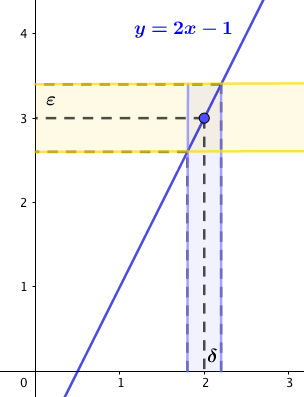
\includegraphics[width=0.2
			\textwidth]{imagenes/imagenes03/T03IM08.png}
		\end{figure}
		
		Cuando decimos que $\underset {x\to 2}{lim}\;{2x-1}=3$, queremos decir que nos podemos acercar tanto como queramos a $3$. 
		
		Si por ejemplo nos queremos acercar más que una pequeña cantidad $\varepsilon>0$, tendremos que encontrar el $\delta_{\varepsilon}$ que nos lo garantice. Así:
		\end{multicols}
		
		$|f(x)-3|=|(2x-1)-3|<\varepsilon; \quad |2x-4|<\varepsilon; \quad 2|x-2|<\varepsilon \quad \Rightarrow \quad |x-2|<\varepsilon/2=\delta$. Basta con tomar $\delta=\varepsilon/2$.
			
		

		\end{ejem}
		
		
		\begin{ejem} Comprueba, usando la definición de límite, que $\underset {x\to 1}{lim}\;{5x-3}=2$
		
			 $\underset {x\to 1}{lim}\;{5x-3}=2 \longleftrightarrow  \forall \varepsilon>0,\; \exists \delta_{\varepsilon}>0:\quad 0<|x-1|<\delta \Rightarrow |f(x)-2|<\varepsilon$
			
			$|f(x)-2|=|(5x-3)-2|=|5x-5|=5|x-1|<\varepsilon \Rightarrow |x-1|<\varepsilon/5=\delta$. 
			
			Basta tomar $\delta=\varepsilon/5$ para asegurarnos de separarnos del límite, $2$, menos que la cantidad prefijada $\varepsilon$. Si, por ejemplo quisiéramos estar a menos de $5$ millonésimas de $2$ con $f(x)$, bastaría tomar números $x$ que se alejen del $1$ menos de una millonésima.
		\end{ejem}
		
		\begin{ejem} Un ejemplo algo más complicado.
		Demuestra que $\underset{x\to 1}{lim}\;{\dfrac{2x}{2x^2-x-3}}=-1$
		
		Si $f(x)=\dfrac{2x}{2x^2-x-3} = \dfrac {2x}{(x+1)(2x-3)},\; x\neq-1; x\neq 3/2$, debemos probar que:
		
		$\forall \varepsilon>0,\; \exists \delta>0: \mbox{ si } x\in Dom(f)\sim \{ 1, -1, 3/2\}$ y si $0<|x-1|<\delta \to$ 
		
		
		\hspace{10mm}
		$\to\left| \dfrac{2x}{2x^2-x-3}-(-1) \right|<\varepsilon$
			
		 Para determinar $\delta$ en función de $\varepsilon$ partiremos de $|f(x)-L|$ para transformarla en factores que contengan a $|x-1|$ y $|g(x)|$, que deberemos acotar.
		
		 $\left| \dfrac{2x}{2x^2-x-3}+1 \right|= \left| \dfrac{(2x+3)(x-1)}{(x+1)(2x-3} \right|=\left| \dfrac{(2x+3)}{(x+1)(2x-3)} \right|\cdot |x-1|=|g(x)|\cdot|x-1|$
		
		Tenemos:  $0<|x-1|<\delta \to |g(x)|\cdot|x-1|<\varepsilon$
		
		 Ahora procederemos a la búsqueda apropiada de una $\delta$ para acotar $|g(x)|$.
		
		Como $x+1=0$ y $2x-3=0$ son dos \emph{asíntotas verticales} de la función $f$ (hacen que f se dispare al $\infty$) y siendo $x=3/2$ el punto más próximo a $x_0=1$ (el otro, $x=-1$ es más lejano), elegiremos $\delta_1=\frac 1 2 |\frac 3 2 - 1|=\frac 1 4$
		
		 Tenemos ahora que si $|x-1|<\delta<\delta_1 \to |x-1|<\frac 1 4 \leftrightarrow -\frac 1 4 < x-1 < \frac 1 4 \leftrightarrow \frac 3 4 < x < \frac 5 4$
		
		 Ahora acotaremos cada uno de los factores de $g(x)$:
		
		\begin{itemize}
		
			\item [*] $\frac 3 2 < 2x < \frac 5 2 \leftrightarrow \frac 9 2 < 2x+3 < \frac {11} {2} \to |2x+3|<\frac {11}2$
			\item [*] $\frac 3 2 < 2x < \frac 5 2 \leftrightarrow -\frac {3} 2 < 2x-3 < -\frac {11} {2} \leftrightarrow -2 < \dfrac {1}{2x-3}< -\frac {2}{3}\to \left| \dfrac {1}{2x-3} \right|<2$
			\item [*] $\frac 7 4 < x+1 < \frac 9 4 \leftrightarrow \frac 4 9 < \dfrac {1}{x+1} < \frac 4 7 \to \left| \dfrac {1}{x+1} \right| <\frac 4 7$
		\end{itemize}
		
		Entonces: $|g(x)|= \dfrac {|2x+3|}{|x+1|\cdot |2x-3|}< \frac {11}2 \cdot 2 \cdot \frac 4 7 = \frac {44} 7 \to |g(x)|<\frac {44} 7 =M$
		
		 Luego: $0<|x-1|<\delta \to \frac {44} 7 |x-1|< \varepsilon \to |x-1|<7\varepsilon/44=\delta_2$
		
		 Por tanto, eligiendo $\delta=min\{1/4,\; 7\varepsilon/44\}$ se tiene que:
		
		 $0<|x-1|<\delta \to \dfrac{|2x+3|}{|x+1|\cdot |2x-3|}<\frac {44}{7} \mbox { y } |x-1|<\frac {7\varepsilon}{44} \to $
		
		 $\to \dfrac{|2x+3|}{|x+1|\cdot |2x-3|}|x-1|<\frac {44}{7} \frac {7\varepsilon}{44}=\varepsilon$,
		
		 
		\hspace{20mm}Es decir: $ \left| \dfrac{2x}{2x^2-x-3}-(-1)  \right|<\varepsilon \qquad \qquad \qquad \qquad c.q.d.$
		\end{ejem}
		
		
		\begin{ejem} Demostración del teorema del límite de la suma visto en álgebra de límites.
		
		Sean $L, M,  \in \mathbb R \quad $, con $\quad \underset {x \to x_0}{lim}{f(x)}=L; \; \underset {x \to x_0}{lim}{g(x)}=M \quad \Rightarrow$

		
		$\Rightarrow \underset {x\to x_0}{lim}{(f(x)+g(x))}=\underset {x\to x_0}{lim}{f(x)}+\underset {x\to x_0}{lim}{g(x)}=L+M$
			
		\end{ejem}

		\begin{proof}[]%\renewcommand{\qedsymbol}{$\diamond$}
		Hemos de probar que dado $\varepsilon >0, \exists \delta>0$ tal que para todo $x: \; 0<|x-x_0|<\delta $, entonces se cumple que $| \left( f(x)+g(x) \right)- (L+M)|<\varepsilon$	
		
		Sea $\varepsilon'=\varepsilon/2$, por definición:
		
		 $\underset{x\to x_0}{lim}\;{f(x)}=L \leftrightarrow \forall \varepsilon'>0, \exists \delta_1>0: 0<|x-x_0|<\delta_1 \to |f(x)-L|<\varepsilon'$
		 
		 y $\underset{x\to x_0}{lim}\;{g(x)}=M \leftrightarrow \forall \varepsilon'>0, \exists \delta_2>0: 0<|x-x_0|<\delta_2 \to |g(x)-M|<\varepsilon'$
		 
		 Sea, ahora, $\delta=min\{\delta_1, \delta_2 \}$, entonces, para todo $x:\; 0<|x-x_0|<\delta$ se cumplirá que:
		 
		 $|f(x)-L|<\varepsilon'$ y $|g(x)-M|<\varepsilon'$ , entonces:
		 
		 $|f(x)-L|+|g(x)-M|<\varepsilon'+\varepsilon'=2\varepsilon'=\varepsilon$ 
		 
		 Por lo que: $|(f(x)+g(x))-(L+M)|= |(f(x)-L)+(g(x)-M)|\le(*)$
		 
		 $\le |f(x)-L|+|g(x)+L|<\varepsilon\qquad $(*) Desigualdad triangular.
		\end{proof}
		
		\begin{ejem} Demostración del teorema de la conservación del órden.
			
			Si $f(x) \le g(x)$  para todo $x$ en algún intervalo abierto que contenga a $x_0$, excepto posiblemente en el propio $x_0$, y existen los límites de $f(x)$ y de $g(x)$ cuando $x\to x_0$, ($M \mbox{ y }L$)entonces: $\underset {x\to x_0}{lim}{f(x)} \le \underset {x\to x_0}{lim}{g(x)}$, es decir $L<M$
		\end{ejem}
		\begin{proof}[]%\renewcommand{\qedsymbol}{$\diamond$}
		Usaremos el método de demostración por \emph{reducción al absurdo}: Supongamos que $L>M$.
		
		De acuerdo con el teorema de álgebra de límites acerca del límite de la resta: 	$\underset {x\to x_0}{lim}\;{g(x)-f(x)}=M-L$, en consecuencia, $\forall \varepsilon>0, \exists \delta>0: |(g(x)-f(x)-(M-L)|<\varepsilon$, siempre que $0<|x-x_0|<\delta$
		
		Como por hipótesis $L-M>0$, tomaremos $\varepsilon=L-M$ y con $\delta>0$ de modo que:
		
		$|(g(x)-f(x)-(M-L)|<L-M$, siempre que $0<|x-x_0|<\delta$.
		
		Como $a\le|a|$, para cualquier número real $a$, tenemos:
		
		$(g(x)-f(x))-(M-L)<L-M$, con $0<|x-x_0|<\delta$, que se simplifica en: $g(x)<f(x)$ siempre que $0<|x-x_0|<\delta$. Pero esto \emph{contradice} $f(x)\le g(x)$, por lo que la desigualdad $L>M$ es falsa. En consecuencia: $L\le M$
		\end{proof}
	
	\begin{defi}Definición (rigurosa) de límites laterales.
	
	$\underset{x\to x_0^+}{lim}\;{f(x)}=L \leftrightarrow \forall \varepsilon>0, \exists \delta>0: x_0<x<x_0+\delta \to |f(x)-L|<\varepsilon$
	
	$\underset{x\to x_0^-}{lim}\;{f(x)}=L \leftrightarrow \forall \varepsilon>0, \exists \delta>0: x_0-\delta<x<x_0 \to |f(x)-L|<\varepsilon$
	
		
	\end{defi}

	

	\begin{defi} Definición (rigurosa) de límite infinito de una función en un punto.
	
	 $\underset {x\to x_0}{lim}\; {f(x)}=+\infty \leftrightarrow \forall k \in \mathbb R,\; \exists \delta>0: 0<|x-x_0|<\delta \to f(x)>K $	
	
	 $\underset {x\to x_0}{lim}\; {f(x)}=-\infty \leftrightarrow \forall k \in \mathbb R,\; \exists \delta>0: 0<|x-x_0|<\delta \to f(x)<K $	
	\end{defi}
	
	\begin{ejem} Demuestra que $\underset {x\to 1}{lim}\;{\dfrac {1}{(x-1)^2}}=+\infty$
	
	Hemos de demostrar que $\forall K \in \mathbb R , \exists \delta>0: 0<|x-1|<\delta \to \dfrac {1}{(x-1)^2}>K$
	
	Pero $\dfrac {1}{(x-1)^2}>K \leftrightarrow (x-1)^2 < \dfrac 1 K$. Por otra parte, si $0<|x-1|<\delta$, será $|x-1|^2<\delta^2$, de donde $\dfrac {1}{|x-1|^2}>\dfrac {1}{\delta^2}$.
	
	Basta tomar $\delta^2<\dfrac 1 K$, o lo que es lo mismo, $\delta < \dfrac {1}{\sqrt{K}}$ para que si $0<|x-1|<\delta \to \dfrac {1}{|x-1|^2}>\dfrac 1 {\delta^2} > K $
	
	
	\end{ejem}

	
	\begin{defi} Definición (rigurosa) de límite finito de una función en el infinito.
	
	 $\underset {x\to +\infty}{lim}\; {f(x)}=L \leftrightarrow \forall \varepsilon>0 \, , \, \exists K>0: x>K: |f(x)-L|<\varepsilon$
	
	 $\underset {x\to +
	-\infty}{lim}\; {f(x)}=L \leftrightarrow \forall \varepsilon>0 \, , \, \exists  K<0: x<K: |f(x)-L|<\varepsilon$
	\end{defi}
	
	\begin{defi}Definición (rigurosa) de límite infinito en el infinito.
	
	$\underset {x\to +\infty}{lim}\;{f(x)}=+\infty \leftrightarrow \forall K\in \mathbb R, \exists \delta>0: x>\delta \to f(x)>K $
	
	$\underset {x\to +\infty}{lim}\;{f(x)}=-\infty \leftrightarrow \forall K\in \mathbb R, \exists \delta>0: x>\delta \to f(x)<K $
	
	$\underset {x\to -\infty}{lim}\;{f(x)}=+\infty \leftrightarrow \forall K\in \mathbb R, \exists \delta>0: x<\delta \to f(x)>K $
	
	$\underset {x\to -\infty}{lim}\;{f(x)}=-\infty \leftrightarrow \forall K\in \mathbb R, \exists \delta>0: x<\delta \to f(x)<K $
		
	\end{defi}
	
	\section{Continuidad}
	
	Informalmente hablando, una función $f$ definida sobre un intervalo $I$ es \emph{continua} si la curva que la representa, es decir el conjunto de los puntos $(x, f(x))$, con $x \in I$, `se puede dibujar sin levantar el lapiz del papel', sin `hoyos' ni `saltos'.
	
		\begin{figure}[H]
			\centering
			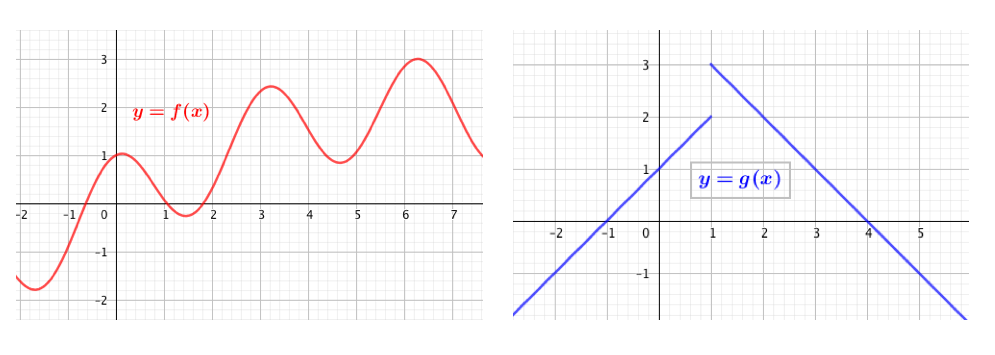
\includegraphics[width=1\textwidth]{imagenes/imagenes03/T03IM09.png}
			\caption{$f$ es continua, pero $g$ no lo es.}
		\end{figure}
	
	La \emph{continuidad}, en matemáticas, es una \emph{condición local}, es decir, una función es o no continua en un punto. Después extenderemos el concepto de continuidad a un intervalo diciendo que la función será continua en él si lo es en todos los puntos que los forman.
	
	\begin{defi} \label{def-ctndad} Continuidad de una función en un punto.
	
	Decimos que $f(x)$ es continua en $x_0\in Dom(f)$ si $\boxed{ \; \underset{x\to x_0}{lim}\;{f(x)}=f(x_0)\; }$ , es decir, 
	
	si $\forall \varepsilon>0, \exists \delta>0: 0<|x-x_0|<\delta \to |f(x)-f(x_0)|<\varepsilon$
		
	\end{defi}

	Esta definición, a la hora de aplicarla en la práctica al estudio de la continuidad de funciones, se traduce en `\underline{el método de los tres pasos}':
	
	$f(x)$ continua en $x_0$ si:
	
	\hspace{10mm} 1) $\exists f(x_0)$

	\hspace{10mm} 2) $\exists \underset{x\to x_0}{lim}\;{f(x)}$	
	
	\hspace{10mm} 3) $f(x_0)=\underset{x\to x_0}{lim}\;{f(x)}$
	
	\begin{defi}Discontinuidades.
	
	Si $f(x)$ no es continua en $x_0$, decimos que es `discontinua' en él.
	
	\vspace{4mm}TIPOS DE DISCONTINUIDADES: Aunque existen varios tipos de clasificar las discontinuidades según autores distintos, daremos como discontinuidades la siguiente clasificación:
	
	\begin{itemize}
		\item Discontinuidad evitable: $\exists f(x_0);\; \exists \underset{x\to x_0}{lim}\;{f(x)}; \mbox{ pero }f(x_0)\neq\underset{x\to x_0}{lim}\;{f(x)}$
		\item Discontinuidad de salto (finito): $\nexists \underset{x\to x_0}{lim}\;{f(x)} \mbox{ porque } \underset{x\to x_0^-}{lim}\;{f(x)}\neq \underset{x\to x_0^+}{lim}\;{f(x)}$. 
		
		Es decir, los límites laterales existen ambos, son finitos, pero distintos.
		\item Discontinuidad asintótica: $\underset{x\to x_0}{lim}\;{f(x)}=\infty$
		\item Discontinuidades de segunda especie: otros casos distintos a los anteriores.
	\end{itemize}
		
	\end{defi}

	\begin{figure}[H]
		\centering
		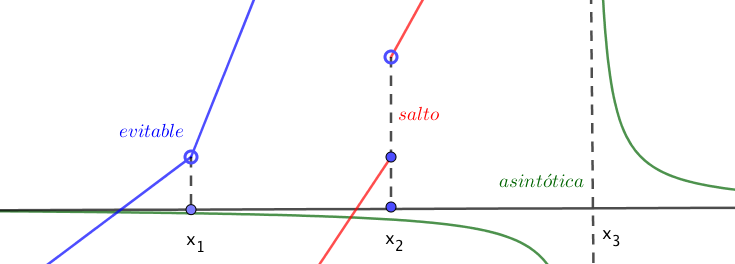
\includegraphics[width=0.7\textwidth]{imagenes/imagenes03/T03IM10.png}
		\caption{Tipos de discontinuidades.}
	\end{figure}

	\begin{defi}Continuidad lateral.
	
		$f(x)$ es continua por la derecha en $x_0$ si $\underset {x\to x_0^+}{lim}\;{f(x)}=f(x_0)$
		
		$f(x)$ es continua por la izquierda en $x_0$ si $\underset {x\to x_0^-}{lim}\;{f(x)}=f(x_0)$
		
	\end{defi}

	\begin{defi}Continuidad en un intervalo.
	
	$f(x)$ es continua en un intervalo abierto $]a,b[$ si lo es $\forall x \in ]a,b[$
	
	$f(x)$ es continua en un intervalo cerrado $[a,b]$ si lo es en el intervalo abierto $]a,b[$ y es continua por la derecha en $a$ y continua por la izquierda en $b$
		
	\end{defi}
	
	\subsection{Continuidad de las funciones elementales}
	
	\begin{teor} Álgebra de funciones continuas.
	
	Sean $f$ y $g$ dos funciones continuas en $x_0$, entonces, las siguientes combinaciones son continuas en $x_0$:
	
	\begin{enumerate}
		\item Sumas: $f+g$
		\item Restas: $f-g$
		\item Productos $f\cdot g$
		\item Producto por constantes: $k\cdot f; \quad \forall k\in \mathbb R$
		\item Cocientes: $f/g$, siempre que $g(x_0)\neq 0$
		\item Potencias: $f^{r/s}$, con $r$ y $s$ enteros y f definida en un intervalo que contenga a $x_0$
		\item Composición: si $f$ continua en $x_0$ y $g$ continua en $f(x_0) \to f\circ g$ continua en $x_0$ 
	\end{enumerate}
		
	\end{teor}

	\begin{proof}
		Demostraremos, p.e., la primera de las propiedades:
		
		$\underset {x\to x_0}{lim}\; {(f+g)(x)}=\underset {x\to x_0}{lim}\; {(f(x)+g(x))}=\underset {x\to x_0}{lim}\; {f(x)}+\underset {x\to x_0}{lim}\; {g(x)} =f(x_0)+g(x_0)=(f+g)(x_0)$ Lo que prueba que $(f+g)$ es continua en $x_0$.
	\end{proof}
	
	\vspace{4mm}Continuidad de funciones elementales:
	\begin{itemize}
		\item Las funciones polinómicas son continuas en todo $\mathbb R$
		\item Las funciones racionales son continuas en su dominio. Presentarán discontinuidades cuando se anule el  denominador.
		\item Las funciones radicales son continuas en sus dominios de definición.
		\item Las funciones $\sin x$ y $\cos x$ y sus combinaciones son continuas en todo $\mathbb R$
		\item La función $\tan x$ presenta discontinuidades asintóticas en $x=(2k+1)\dfrac {\pi}{2},\; \forall k\in \mathbb Z$
		\item La función exponencial es siempre continua.
		\item La función logarítmica es continua en su dominio.
	\end{itemize}
	
	\subsection{Asíntotas}
	\label{subsec-asintotas}
	
	Las asíntotas responden del comportamiento infinito de una función en un punto, son las llamadas \emph{asíntotas verticales}. Independientemente de éstas, otras asíntotas responden del comportamiento finito o infinito de una una función en el infinito, son las llamadas \emph{asíntotas horizontales u oblícuas}.
	
	\begin{defi}.
	
	\begin{itemize}
		
		\item Asíntota Vertical (AV): Decimos que $x=x_0$ es AV de $f(x)$ si $\underset{x\to x_0}{lim}\;{f(x)}=\infty$. Suelen ser valores que anulan el denominador de la función.
		
		Independientemente de que existan o no AV, llamamos:
		
		\item Asíntota Horizontal (AH): Decimos que la recta horizontal $y=b\in \mathbb R$ es AH de $f(x)$ si $\underset{x\to \infty}{lim}\;{f(x)}=b$
		
		En el caso de que no existan AH, puede que la función en el infinito se comporte según una recta oblícua, $y=mx+n$, donde $m$ y $n$ se calculan como se indica a continuación:
		
		\item Asíntota Oblícua (AO) [ si no hay AH]: Decimos que la recta $y=mx+n$ es AO de $f(x)$ si $\underset{x\to x_0}{lim}\;{\dfrac {f(x)} {x} }=m\in \mathbb R$ y $\underset{x\to x_0}{lim}\;{(f(x)-mx)}=n \in \mathbb R$
	\end{itemize}
		
	\end{defi}
	
	Los polinomios no tienen ningún tipo de asíntota.
	
	Una función puede tener ninguna, una, varias, incluso infinitas asíntotas verticales ($y=\tan x$) y las funciones jamás podrán cortar a las asíntotas verticales. En cambio, las funciones pueden tener o no asíntotas horizontales u oblícuas, solo una de ellas o ninguna (aunque pueden ser dos distintas cuando $x\to +\infty$ o $x\to -\infty$) y la función puede cortarla en múltiples ocasiones.

	\begin{figure}[H]
			\centering
			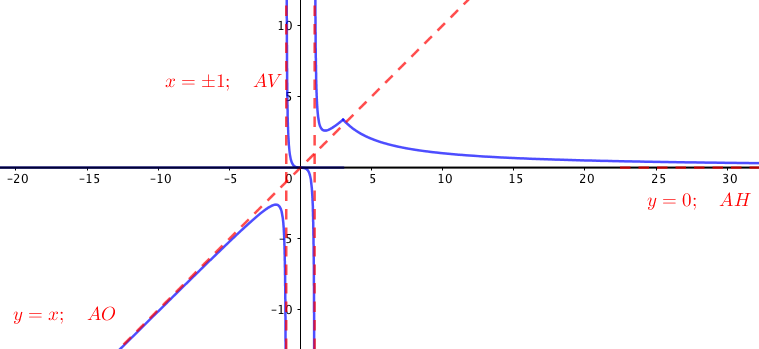
\includegraphics[width=0.75
			\textwidth]{imagenes/imagenes03/T03IM15.png}
		\end{figure}
	
	
	\section{Ejercicios de continuidad}
	\subsection{Ejercicios resueltos de continuidad}
	
	
	
	\begin{ejre} Clasifica las discontinuidades de la  función:  $f(x)=\dfrac {x^3-2x^2+x-2}{x^2-x-2} $
		
	\end{ejre}
	
	\begin{proofw}\renewcommand{\qedsymbol}{$\diamond$}
	
	$x^2-x-2=0 \to x=-1 \wedge x=2$
	
	\begin{itemize}
		\item Continuidad en x=2:
		
		$1) \quad \nexists f(2)=0/0$
		
		$2) \quad \underset{x\to 2}{lim}\; {f(x)}=[0/0;\; mbox{ind.}] =\underset{x\to 2}{lim}\; {\dfrac {(x^2+1)\cancel{(x-2)}}{(x+1)\cancel{(x-2)}}}=\underset {x\to 2}{lim}\; {\dfrac {x^2+1}{x+1}}=5/2$
		
		$3) $ no coinciden
		
		Luego $f(x)$ en $x=2$ es \emph{discontinua evitable}.
		
		\item Continuidad en $x=-1$
		
		$1)\quad \nexists f(1)=-6/0$
		
		$2) \quad \underset {x\to -1}{lim}\; {f(x)}=-6/0=\infty$
		
		$3) $ no coinciden
		
		Luego $f(x)$ en $x=-1$ presenta una \emph{discontinuidad asintótica}.
		\item $\forall x\in \mathbb R \sim \{-1,2 \}$, la función es continua.
	
	\end{itemize}
		
	\end{proofw}
	
	\begin{ejre} Calcula las continuidad de $f(x)=\left\{ \begin{matrix} \dfrac{x+2}{x^2-4} & x\neq -2 \\ k & x=-2 \end{matrix} \right. $
		
	\end{ejre}
	
	\begin{proofw}\renewcommand{\qedsymbol}{$\diamond$}
	
	Hemos de estudiar la continuidad en el nexos de la función, $x=-2$ y, también, en $x=2$ puesto que anula un denominador.
	
	\begin{itemize}
		\item Continuidad en x=2
		
		$1)\quad \nexists f(2)=4/0$
		
		$2)\quad \underset {x\to 2}{lim}\;{\dfrac {x+2}{x^4-4}}=4/0=\infty$
		
		$3)$ no coinciden
		
		$f(x)$ en $x=2$ tiene una \emph{discontinuidad asintótica}
		
		\item Continuidad en $x=-2$
		
		$1)\quad f(-2)=k$
		
		$2) \quad \underset {x\to -2}{lim}\;{\dfrac {x+2}{x^4-4}}=[0/0 \mbox{ind}]=\underset {x\to -2}{lim}\;{\dfrac {\cancel{(x+2)}}{\cancel{(x+2)}(x-2)}}=\underset {x\to -2}{lim}\;{\dfrac {1}{x-2}}=-1/4$
		
		$3) \quad $ si $k=-1/4$, $f(x)$ \emph{continua} en $x=-2$, pero si $k\neq -1/4$, entonces $f(x)$ tendrá una \emph{discontinuidad evitable} en $x=-2$
		
	\end{itemize}
		
	\end{proofw}
	
	\begin{ejre} Calcula la continuidad de $f(x)=\dfrac {x}{\ln (x-2)}$
		
	\end{ejre}
	
	\begin{proofw}\renewcommand{\qedsymbol}{$\diamond$}
	
	Es fácil comprobar que $Dom(\ln (x-2))=]2,+\infty[$, pero el denominador se anula cuando $\ln(x-2)=0 \to x-2=e^0=1 \to x=3$. Hemos, pues, de estudiar la continuidad en x=3, en el resto del domino, la función es continua.
	
	$1)\quad \nexists f(3)=3/0$
	
	$2)\quad \underset {x\to 3}{lim}\; {f(x)}=3/0=\infty$
	
	$3) $ no coinciden, $f(x)$ en $x=3$ tiene una \emph{discontinuidad asintótica}.
	
	Luego $f(x)$ es ctna. $\forall x \in ]2,+\infty[\, \sim \{3\}$, presentando en $x=3$ una discontinuidad asintótica. 
	
		
	\end{proofw}
	
	
	\begin{ejre} Estudia la continuidad de $f(x)=\left\{ \begin{matrix} 
	|x+2| & x<-1 \\ 
	x^2 & -1\le x < 1 \\
	2x+1 & x>1 
	\end{matrix} \right. $	
	\end{ejre}

	\begin{proofw}\renewcommand{\qedsymbol}{$\diamond$}
	
	$f(x)=\left\{ \begin{matrix} 
	|x+2| & x<-1 \\ 
	x^2 & -1\le x < 1 \\
	2x+1 & x>1 
	\end{matrix} \right. = 
	\left\{ \begin{matrix} 
	-x-2 & x<-2 \\
	x+2 & -2\le x<-1 \\ 
	x^2 & -1\le x < 1 \\
	2x+1 & x>1 
	\end{matrix} \right.$

		Puesto que no hay ningún denominador que se anule, solo hemos de estudiar la continuidad en los nexos de la función: $x=\{-2, -1, 1 \}$. En el resto de números reales la función es continua.
		
		\begin{itemize}
			\item Continuidad en $x=-2$
			
			$1) \quad \exists f(-2)=(-2)+2=0$
			
			$2) \quad \exists \underset{x\to -2^-}{lim}\;{f(x)}= \underset{x\to -2^-}{lim}\;{-x-2}=-(-2)-2=0;\qquad \exists \underset{x\to -2^+}{lim}\;{f(x)}= \underset{x\to -2^+}{lim}\;{x+2}=(-2)2=0 \quad \Rightarrow \quad \exists \underset{x\to -2}{lim}\;{f(x)}=0$
			
			$3) $ Coinciden, luego $f(x)$ es \emph{continua} en $x=-2$
			
			\item Continuidad en $x=-1$ 
			
			$1)\quad f(-1)=(-1)^2=1$
			
			$2) \quad \underset {x\to -1^-}{lim}\; {x+2}=-1+2=1; \qquad \underset {x\to -1^-}{lim}\; {x^2}=(-1)^2=1 \quad \Rightarrow \quad \exists \underset{x\to -1}{lim}\;{f(x)}=1$
			
			$3) $ Coinciden, luego $f(x)$ es \emph{continua} en $x=-1$
			
			\item Continuidad en $x=1$
			
			$1)\quad \nexists f(1)$
			
			$2) \quad \underset {x\to 1^-}{lim}\; {x^2}=1; \qquad \underset {x\to 1^+}{lim}\; {2x+1}=3 \quad \Rightarrow \quad \nexists \underset{x\to 1}{lim}\;{f(x)}$ Los límites laterales son finitos y distintos.
			
			$3) $ No coinciden. $f(x)$ tiene una \emph{discontinuidad de salto} en $x=1$
			
			
		\end{itemize}
		
	
	\end{proofw}
	
	\begin{ejre}Estudia las asíntotas de $f(x)=\dfrac {3x-1}{x+2}$
		
	\end{ejre}
	
	\begin{proofw}\renewcommand{\qedsymbol}{$\diamond$}
		
		$\underset {x\to -2}{lim}\;{\dfrac {3x-1}{x+2}}=-7/0=\infty \to x=-2$ AV
		
		$\underset {x\to \infty }{lim}\;{\dfrac {3x-1}{x+2}}=3\to y=3$ AH (luego $\nexists$ AO) 
		
	\end{proofw}

	\begin{ejre} Estudia las asíntotas de $f(x)=\dfrac {x^3+4x^2}{x^2+1}$
		
	\end{ejre}
	
	
	\begin{proofw}\renewcommand{\qedsymbol}{$\diamond$}
	
	$\nexists x_0 \; / \; \underset {x\to x_0}{lim}\;{f(x)}=\infty$, ya que $x^2+1\neq 0, \; \forall x$. Luego $\nexists$ AV
	
	$\underset {x\to \infty}{lim}\;{f(x)}=\infty$, ya que el numerador es de grado mayor al denominador, por ello $\nexists$ AH. Veamos si $\exists$ AO: $y=mx+n$
	
	$m=\underset {x\to \infty}{lim}\;{\dfrac {f(x)}{x}}=\underset {x\to \infty}{lim}\;{\dfrac {x^3+4x^2}{x^3+x}}=1$. 
	
	Busquemos ahora $n=\underset {x\to \infty}{lim}\;{\left(\, f(x)-1\cdot x \right)}=\underset {x\to \infty}{lim}\;{ \left( \dfrac {x^3+4x^2}{x^2+1}-x \right) }=\underset {x\to \infty}{lim}\;{\dfrac {4x^2-x}{x^2+1}=4}\to $ 
	
	$\to y=x+4$ es la AO.
		
	\end{proofw}
	
	\begin{ejre} Estudia las asíntotas de $f(x)=\dfrac {x^4}{x^2+1}$
		
	\end{ejre}
	
	\begin{proofw}\renewcommand{\qedsymbol}{$\diamond$}
	
	Como $x^2+1\neq 0 \to \nexists$ AV
	
	Como $\underset {x\to \infty}{lim}\;{f(x)}=\infty \to \nexists $ AH
	
	Como $\underset {x\to \infty}{lim}\;{\dfrac {f(x)}{x}}=\underset {x\to \infty}{lim}\;{\dfrac {x^4}{x^3+x}}=\infty \to \nexists m \to \nexists $ AO
	
	Esta función no tiene ningún tipo de asíntota.
	
	\end{proofw}
	
	
	
	\begin{ejre} Calcula las asíntotas de la función $f(x)=\sqrt{
	x^2-2x}$
		
	\end{ejre}
	
	\begin{proofw}\renewcommand{\qedsymbol}{$\diamond$}
	
	Es fácil comprobar que la función no tiene ni asíntotas verticales ni horizontales y que su dominio es $]-\infty,0]\cup[2,\infty[$. Veamos pues sus asíntotas oblícuas, en plural, porque la raíz puede tener comportamiento distinto en $\pm \infty$.
	
	*  AO cuando $x\to +\infty$: $\quad y=mx+n$
	
	$m=\underset {x\to +\infty}{lim}\; {\dfrac {\sqrt{x^2-2x}}{x}}=1$; $\quad n=\underset {x\to +\infty}{lim}\; {(\sqrt{x^2-2x}-x)}=[\infty - \infty: \mbox{conjugado}]= \underset {x\to +\infty}{lim}\; {\dfrac {-2x}{\sqrt{x^2-2x}+x}}=\dfrac {-2}{1+1}=-1$; $\qquad y=x-1:$ AO ($x\to +\infty$).
	
	\vspace{3mm}* AO cuando $x\to -\infty$: $\quad y=mx+n$
	
	$m=\underset {x\to -\infty}{lim}\; {\dfrac {\sqrt{x^2-2x}}{x}}=[x=-t]=\underset {t\to +\infty}{lim}\; {\dfrac {\sqrt{t^2+2t}}{-t}}=-1$; $\quad n=\underset {x\to -\infty}{lim}\; {(\sqrt{x^2-2x}+x)}=
	[x=-t]=\underset {t\to +\infty}{lim}\; {(\sqrt{t^2+2t}-t)}=[\infty - \infty: \mbox{conjugado}]= \underset {t\to +\infty}{lim}\; {\dfrac {2t}{\sqrt{t^2+2t}+t}}=\dfrac {2}{1+1}=1$; $\qquad y=-x+1:$ AO ($x\to -\infty$).
	
	
		
	\end{proofw}
	
		
	\begin{ejre} Calcula las asíntotas de $f(x)=\dfrac {|x|}{x+1}$
		
	\end{ejre}
	
	\begin{proofw}\renewcommand{\qedsymbol}{$\diamond$}
	
	Obviamente, $f(x)$ es una función definida a trozos:
	
		\begin{equation*}
		f(x)=
		\begin{cases} 
		\;\;  \dfrac {-x}{x+1} &\mbox{si } x< 0 \\ 
		\; \dfrac {x}{x+1} & \mbox{si } x \ge 0 
		\end{cases}
		\end{equation*}
		
		$\underset {x\to -1}{lim}\; {f(x)}= \underset {x\to -1}{lim}\; {\dfrac {-x}{x+1}}=-1/0=\infty \qquad x=-1$: AV
		
		$\underset {x\to +\infty}{lim}\;{f(x)}= \underset {x\to +\infty}{lim}\;{\dfrac {x}{x+1}}=1 \qquad y=1$: AH $(x\to +\infty)$
		
		$\underset {x\to -\infty}{lim}\;{f(x)}= \underset {x\to -\infty}{lim}\;{\dfrac {-x}{x+1}}=[x=-t]=\underset {t\to +\infty}{lim}\;{\dfrac {t}{-t+1}}=-1 \qquad y=-1$: AH $(x\to -\infty)$
		
		
		
	\end{proofw}
	
	\begin{ejre} Demostrar que la función de Diriclhet (figura \ref{fig:dirichlet}) no es continua en ningún punto.
	
	\begin{equation*}
		f(x)=
		\begin{cases} 
		\;\;  0 &\mbox{if } x \in \mathbb{Q} \\ 
		\; 1 & \mbox{if } x \in \mathbb{R} \sim \mathbb{Q} 
		\end{cases}
		\end{equation*}
		
	\end{ejre}

	\begin{proofw}\renewcommand{\qedsymbol}{$\diamond$}
		
		Sea $x_0 \in \mathbb Q$, siempre podemos construir una sucesión de números irracionales $ \{ \alpha_n \} \to x_0$, pero entonces, al acercarnos a $x_0$ con estos números irracionales, $f(\alpha_n)=1, \; \forall n$, al ser $\alpha_n$ irracionales. es decir: $\underset{\alpha_n \to x_0}{lim}\;{f(x)}=1\neq f(x_0)=0$, por ser $x_0$ racional. Luego $f(x)$ no puede ser continua en ningún número racional.
		
		Sea $x_1 \in \mathbb R \sim \mathbb Q$, siempre podemos construir una sucesión de números racionales $ \{ \beta_n \} \to x_1$, pero entonces, al acercarnos a $x_1$ con estos números racionales, $f(\beta_n)=0, \; \forall n$, al ser $\beta_n$ racionales. es decir: $\underset{\beta_n \to x_1}{lim}\;{f(x)}=0\neq f(x_1)=1$, por ser $x_1$ irracional. Luego $f(x)$ no puede ser continua en ningún número iracional.
		
		Conclusión: f(x) no es continua en ningún número real.
		
	\end{proofw}

	
	
	
	
	\subsection{Ejercicios propuestos de continuidad}
	
	\emph{Los ejercicios de cálculo de asíntotas los dejaremos para cuando estudiemos el tema de `representación gráfica de funciones explícitas'.}
	
		\begin{enumerate}[1).-  ]
		
		\item Estudia la continuidad de $f(x)=\dfrac {x^3-2x^2-3x}{x^2-x-6}$
		
		\rightline{\textcolor{gris}{Solución: $x=-2$ asintótica; $x=3$ evitable.}}
		
		\item Calcula las continuidad de $f(x)=\left\{ \begin{matrix} e^{1-x^2} & x\le -1 \\ -\dfrac 1 x & x>-1 \end{matrix} \right. $
		
		\rightline{\textcolor{gris}{Solución: $x=-1$, salto; $x=0$, asintótica}}
		
		\item Calcula el valor de $\quad k \quad$ para que la siguiente función sea continua en todo $\mathbb R$  $\qquad f(x)=\left\{ \begin{matrix} \dfrac{x^3-1}{x-1} & x\neq 1 \\ \ln k & x=1 \end{matrix} \right. $
		
		\rightline{\textcolor{gris}{Solución: $k=e^3$}}
		
		\item Estudia la continuidad de las funciones siguientes:
		
		$a)\quad  f(x)=\left\{ \begin{matrix} e^x & x< 1 \\ \ln x & x\ge1 \end{matrix} \right. $ $\qquad \qquad b)\quad  f(x)=\left\{ \begin{matrix} \dfrac 1 x & x< 1 \\  2x-1 & x\ge1 \end{matrix} \right. $ 
		
		\rightline{\textcolor{gris}{Solución: $a)\quad x=1 \mbox{ salto; }\qquad b) \quad x=0 \mbox{ asintótica; } x=1 \mbox{ continua.}$}}
		
		\item La siguiente función es continua en $]-1,+\infty[$, halla el valor de $a$
		 
		 $f(x)=\left\{ \begin{matrix} x^2-4x+3 & -1<x<0 \\ \dfrac{x^2+a}{x+1} & x\ge0 \end{matrix} \right. $
		 
		 \rightline{\textcolor{gris}{Solución: $a=3$}}
		 
		 \item Calcula el valor de $t$ para que la siguiente función sea continua en $x=2$.
		 
		 $f(x)=\left\{ \begin{matrix} 
		|x-1|-t & x\le -2 \\ 
		x-5 & x>2  
		\end{matrix} \right.$

		\rightline{\textcolor{gris}{Solución: $t=4$}}
		
		\item Encuentra los valores de $a$ y $b$ para que la siguiente función sea continua y si gráfica pase por el origen de coordenadas.
		 
		 $f(x)=\left\{ \begin{matrix} 
		\ln x - 1 & x>1 \\ 
		2x^2+ax+b & x\le 1  
		\end{matrix} \right.$

		\rightline{\textcolor{gris}{Solución: Ayuda, pasar por el origen supone que si $x=0 \to y=0\quad a=3;\; b=0$}}
		
		\item Encuentra los valores de $a$ y $b$ para que la siguiente función sea continua en $\mathbb R$ y pase por el punto $(-1,2)$.
		 
		 $f(x)=\left\{ \begin{matrix} 
		ax^2+b & |x|\le 2 \\ 
		\dfrac {1}{x^2} & |x|>2  
		\end{matrix} \right.$

		\rightline{\textcolor{gris}{Solución:  $a=3/4;\; b=-11/4$}}
		
		
		\item Encuentra el valor de $m$ para que la siguiente función tenga límite finito en $x=3/2$ y calcula su valor:
		$f(x)=\left\{ \begin{matrix} 
		\dfrac {9-mx^2}{3-2x} & x\neq 3/2 \\ 
		1 & x=3/2  
		\end{matrix} \right.$
		
		\rightline{\textcolor{gris}{Solución:  $m=4;\; \mbox{límite}=6$}}
		
		\item .
		
		\begin{figure}[H]
			\centering
			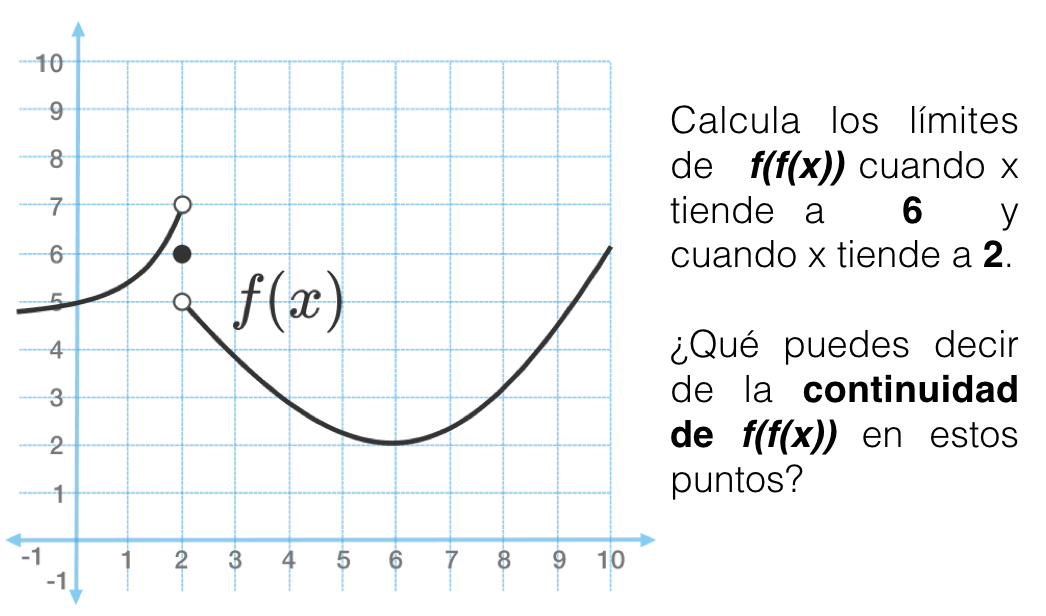
\includegraphics[width=0.75
			\textwidth]{imagenes/imagenes03/T03IM11.png}
		\end{figure}
		
		\rightline{\textcolor{gris}{Solución:  $f(f(6^-))=f(2^+)=5; \quad f(f(6^+))=f(2^+)=5; \quad f(f(6))=6 \quad \mbox{evitable}$}}
		\rightline{\textcolor{gris}{  $f(f(2^-))=f(7^-)=2.5; \quad f(f(2^+))=f(5^-)=2.5; \quad f(f(2))=2 \quad \mbox{evitable}$}}
		
		\item Calcula las asíntotas de a) $f(x)=\dfrac {x^3-x^2+1}{2x^2-x+3} \qquad$ b) $f(x)=\dfrac {x^5+2x^2-5}{x^4-1}$
		
		\rightline{\textcolor{gris}{Solución: a) $y=\frac 1 2 x-\frac 1 4 \quad $ b) $x=\pm 1; \; y=x$ }}
		
		\item Calcula las asíntotas de a) $f(x)=\dfrac {\sqrt{1-x}}{3x} \qquad$ b) $f(x)=\dfrac {x+\sqrt{x^2+1}}{x}$
		
		\rightline{\textcolor{gris}{Solución: a) $x=0; \; y=0 \; (x\to -\infty) \quad$ b) $x=0; \; y=2 \; (x\to +\infty); \; y=0 \; (x\to -\infty)$}}
		
		\item Calcula las asíntotas de a) $y=\ln{\dfrac {x^2-1}{x^2+1}}\qquad$ b) $y= \dfrac {e^x-1}{e^x+1}$
		
		\rightline{\textcolor{gris}{Solución: a) $x=\pm 1; \; y=0\quad$ b)$\nexists AV; \; y=\pm 1 \; (x\to \pm \infty)$ }}
		
		\item Calcula las asíntotas de a) $y=\ln \dfrac {x}{x+1}\qquad$ b) $y=\dfrac {e^{|x-1|}}{x^2+2x-3}$
		
		\rightline{\textcolor{gris}{Solución: a) $x=1^-;\; x=0^+; \; y=0 \quad$ b) $x=-3; \; x=1; \; \nexists AH; \; \nexists AO$}}
		
		\item Considera la función $f(x)=\dfrac {ax+8}{bx+6}$. Encuentra los valores de $a$ y $b$ para que las rectas $x=2$ e $y=-4$ sean, respectivamente, su asíntota vertical y horizontal.
		
		\rightline{\textcolor{gris}{Solución $a=12;\quad b=-3$ }}
		
		\item Hallar $a$ y $b$ para que la siguiente función sea continua en todo $\mathbb R$.
		
		$f(x)=
		\begin{cases}
		a(x-1)2 & \mbox{ si } x\le 0 \\	
		\sin (b+x) & \mbox{ si } 0<x<\pi \\	
		\dfrac \pi x & \mbox{ si } x\ge \pi 
		\end{cases}
		$
	
		\rightline{\textcolor{gris}{Solución: $a=-1; \; b=\dfrac {3\pi}{2}+2k\pi,\; k\in \mathbb Z$ }}
		
		\item Hallar $a$ y $b$ para que la siguiente función sea continua en todo $\mathbb R$.
		
		$f(x)=
		\begin{cases}
		a \; e^{ \dfrac {\sin^2 x}{x} }+b \cos x & \mbox{ si } x< 0 \\	
		6 & \mbox{ si } x=0 \\	
		3a \; \dfrac {\sin x}{x}+b(x-1) & \mbox{ si } x>0 
		\end{cases}
		$
		
		\rightline{\textcolor{gris}{Solución:$a=b=3$}}
		
		\item Estudia la continuidad de la función: $f(x)=\dfrac {e^x}{x^2+k}$
		
		\rightline{\textcolor{gris}{Solución:Si $k>0$, $f$ comtinua en todo $\mathbb R$;}}
		
		\rightline{\textcolor{gris}{Si $k\le 0$, f tiene discont. asintóticas en $x=\pm \sqrt{-k}$ }}
		
		\item Estudia la continuidad de la función: $f(x)=
		\begin{cases}
		1 & \mbox{ si } x=0\\	
		\dfrac {|\sin x|}{x} & \mbox{ si } x \neq 0
		\end{cases}$
		
		\rightline{\textcolor{gris}{Solución:$f$ discontinua de salto en $x=0$ }}
		
		\item Dada la función:  $f(x)=\dfrac {|x-2|}{|x-1|-1}$,
		
		$a) \quad $ Define la función a trozos.
		
		$b) \quad $ Estudia su continuidad.
		
		\rightline{\textcolor{gris}{Solución: hay que romper la función como aprendimos en el ejercicio \ref{ejre:rompe-trozos}.}}
		\rightline{\textcolor{gris}{El denominador se anula para $x=2$ y para $x=0$}}
		\rightline{\textcolor{gris}{$f(x)= \dfrac {x-2}{2} \quad \ si \quad x<1$ }}
		\rightline{\textcolor{gris}{$f(x)=-1 \quad si \quad 1\le x < 2 \sim \{0\}$}}
		\rightline{\textcolor{gris}{$f(x)=1 \quad si \quad x>2$}}
		\rightline{\textcolor{gris}{Continua en $x=1$; discontinua de salto en $x=2$; discontinua asintótica en $x=0$}}
		
		\item Calcula $a$ y $b$ para que la siguiente función sea continua en $\mathbb R$
		
		$f(x)=
		\begin{cases}
		\dfrac 1 {e^x} & \mbox{ si } x\le 0 \\	
		a\; \cos x + b & \mbox{ si } 0< x \le \pi \\
		\sin x - a\; x & \mbox{ si } x> \pi 
		\end{cases}$
	
		\rightline{\textcolor{gris}{Solución: $a=\dfrac 1 {2(\pi - 1)}; \quad b=\dfrac 1 2$}}

		\item Estudia la continuidad de $f(x)=\begin{cases}
		|x+2| & \mbox{ si } 	x<-1 \\
		x^2 & \mbox{ si } 	-1\le x \le 1 \\
		2x+1 & \mbox{ si } 	x>1 
		\end{cases}$ 
		
		\rightline{\textcolor{gris}{Solución: Discontinua de salto en $x=1$}}
	
		\end{enumerate}
		
			
	\section[Propiedades de las funciones continuas en intervalos cerrados] {Propiedades de las funciones continuas en intervalos cerrados \sectionmark{Propiedades funciones continuas}} 
	\sectionmark{Propiedades funciones continuas} 
	
	\label{prop-func-ctnas}


		\begin{figure}[H]
			\centering
			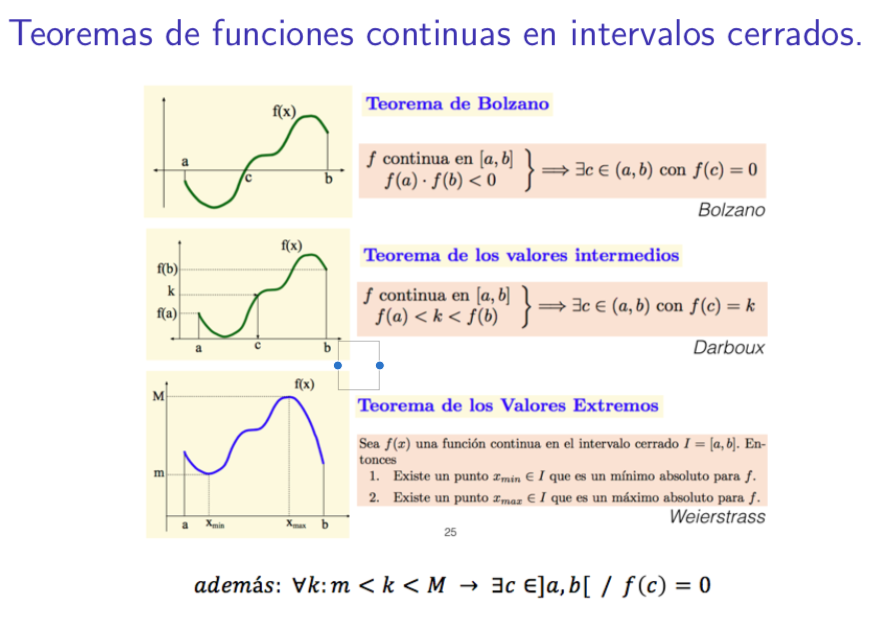
\includegraphics[width=1\textwidth]{imagenes/imagenes03/T03IM12.png}
		\end{figure}
	

	\begin{teor}{Principio de Intervalos Encajados. G. Cantor}.
	
	Sea $I_n$ usa sucesión de intervalos cerrados y encajados, es decir, $I_n=[a_n,b_n];\; I_{n+1}=[a_{n+1},b_{n*1}]$, con $I_{n+1} \subset I_n,; \forall n\in \mathbb N$ y tales que su longitud tiende a cero (se hace cada vez más pequeña): $\underset {n \to +\infty}{lim}\;{long(I_n)} = \underset {n \to +\infty}{lim}\;{(b_n-a_n)} = 0 \quad \Rightarrow \quad \exists \;!\; c\in \mathbb R: \; \underset { n\ge 1 }{ \bigcap  } { \; I_{ n } \; }=\left\{ c \right\} $
		
	\end{teor}
	
	La demostración de este teorema excede de las pretensiones del presente texto y se basa en que toda sucesión monótona y acotada alcanza el supremo o el ínfimo.
	
	
	
	\begin{teor}Teorema de Bolzano: 
		
	
Si f, continua y toma distinto signo en los extremos de un intervalo cerrado, se anula en algún punto intermedio.



 $f : [a,b] \to  \mathbb R,\; continua; \; f(a)\cdot f(b)<0 \Rightarrow \exists \; c \in ]a,b[: \; f(c)=0$ 

	\end{teor}

	\begin{proof}.
	\begin{multicols}{2}
	Dividimos $[a, b]$ por la mitad. Si en el punto medio $f$ vale $0$, hemos concluido. Si no, elegimos, de los dos intervalos en que hemos dividido $[a,b]$ el semiintervalo $[a_1,b_1]$ en cuyos extremos $f$ tiene distinto signo. Lo dividimos de nuevo. . . Repitiendo la operación, obtenemos una sucesión de intervalos encajados $[a_n, b_n]$, de longitud $(b - a)/2n$ que tiende a cero, y , por el \emph{Principio de intervalos encajados de Cantor}, define un punto único $c$ en el que la función es nula. De lo contrario, al ser $f$ continua, $\underset {x\to c}{lim}\; {f (x)} = f (c) \neq 0$ y existirá un entorno de $c$ en el que $f$ toma el signo del límite (Teorema de Conservación del Signo -lema \ref{teor:conserva-signo}-). Pero en todo entorno de $c$ existen puntos en que $f$ es mayor que $0$ y puntos en los que es menor. Entonces, por reducción al absurdo, $f(c) = 0$. 

	\begin{figure}[H]
 		\centering
		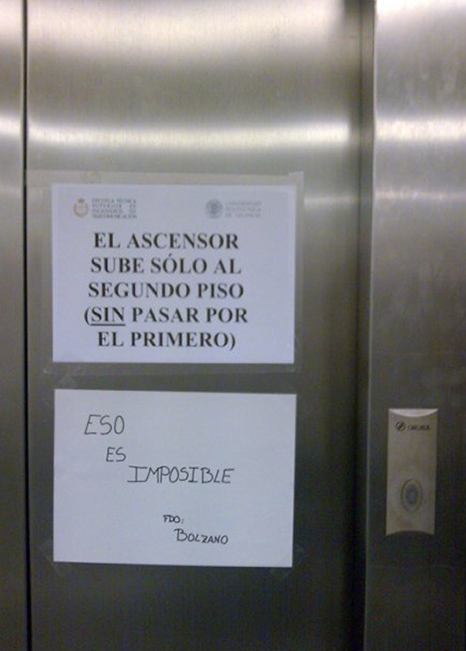
\includegraphics[width=.3\textwidth]{imagenes/imagenes03/xiste03.png}
	\end{figure}
	\end{multicols}

\end{proof}

	OBSERVACIONES SOBRE EL TEOREMA DE BOLZANO:
	
	\begin{itemize}
		\item Geométricamente, el teorema asegura que una curva continua en un intervalo cerrado que tome valores de distinto signo en los extremos del intervalo cortará, al menos una vez, al eje OX.
		\item La condición de continuidad en el intervalo cerrado es totalmente necesaria, sin ella el teorema no tiene por qué cumplirse, como muestra la siguiente figura.
		
		\begin{figure}[H]
 		\centering
			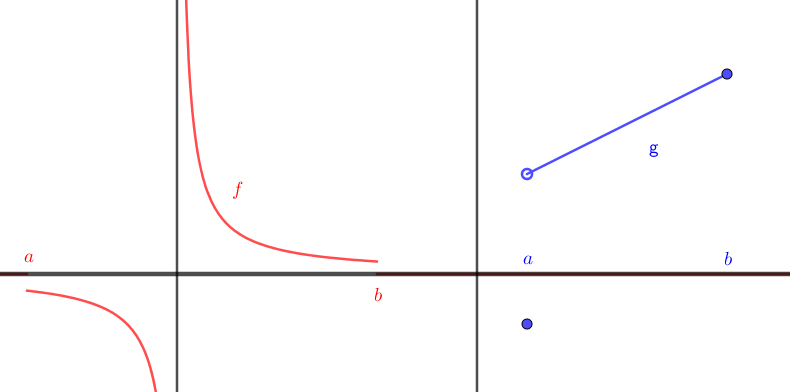
\includegraphics[width=.6\textwidth]{imagenes/imagenes03/T03IM14.png}
			\caption{$f$ no continua en $]a,b[$, tiene una discontinuidad asíntótica en $0\in [a,b]$ ; $g$ no continua en $[a,b]$, discontinua en $a$ por la derecha}
		\end{figure}
		
	\end{itemize}


	\begin{teor} Propiedad de Darboux (del valor intermedio):
	
	 Si $f$, continua en $[a,b]$, tal que toma valores distintos en $a$ y en $b$, entonces toma todos los valores intermedios, al menos una vez, entre $f(a$) y $f(b)$ 
	 
	 $f \mbox{ continua } [a,b], \mbox{supongamos, sin límite de generalidad, que } f(a)<f(b) \rightarrow \forall \; y \; / \; f(a)<y<f(b), \; \exists c \in ]a,b[ : f(c)=y$
	\end{teor}

	\begin{proof}
		
 	Definimos $g(x) = f(x) - y$, que cumple $g(a) < 0, \; g(b) > 0$ $\quad g(a)=f(a)-y <0;\; g(b)=f(b)-y>0 \quad , \mbox{ por hipótesis} $. Entonces, por el teorema de Bolzano, $\exists \; c \in  ]a, b[ \; / \;  g(c) = f (c) - y = 0 \to   f (c) = y$

 	\end{proof}
 


	\begin{teor} Teorema de Weierstrass (o de los valores extremos): 
		
	
	Toda función continua en un intervalo cerrado alcanza en él un máximo y un mínimo. 
	
	\end{teor}
	
	\begin{proof}.
		
	\begin{itemize} 
	
	
	\item [*] $f$ está acotada en $[a, b]$. Supongamos que no. Dividimos $[a, b]$ en dos semiintervalos. Elegimos aquél en que $f$ no está acotada (al menos no lo está en uno de ellos). Lo dividimos de nuevo. . . Repitiendo la operación, obtenemos una sucesión de intervalos encajados que define un punto $\alpha$, tal que $f$ no está acotada en ningún entorno suyo. Pero, al ser $f$ continua, $\underset {x\to \alpha }{lim}\;{f(x)} = f(\alpha)$ y $f$ está acotada en un entorno de  $\alpha$, llegamos a una contradicción.
	
	\item [*] Al ser $f$ acotada en $I = [a, b]$, $f(I)$ tiene supremo $M$ e ínfimo $m$. Veamos que son máximo y mínimo (f los alcanza). En efecto, si $M$ no es alcanzado por $f$, la función $g(x) = \dfrac {1}{M - f(x)}$ será continua en $I$, por lo tanto acotada. Entonces $\exists \; k \; / \;  \dfrac {1}{M-f(x)} < k, \; \forall x \in I \Rightarrow  f(x) < M  - \dfrac 1 k$, y $M$ no sería el supremo. 
	
		Es decir, $x_1,\; x_2 \; \in \;  I \; /\;  f(x1) = m,\;  f(x2) = M $
		
	\end{itemize}

 
 	\end{proof}
 	
	\begin{coro}
 		Una función continua transforma un intervalo cerrado en un intervalo cerrado.
 	\end{coro}
 	
 	\begin{proof}.
 	
 	
 	\begin{itemize}
 		
 	
 	
 	 \item [*] Por el teorema de Weierstrass, $f$ , continua en $[a, b]$, alcanza en él un máximo $M$ y un mínimo $m$.
 	
 	 \item [*] Por la propiedad de Darboux, $f$ alcanzará todos los valores comprendidos entre $m$ y $M$, con lo que $[a, b]$ se transforma en $[m, M]$.
 	 
 	 \end{itemize}
 
 
 	\end{proof}
	
 		\begin{figure}[H]
 		\centering
			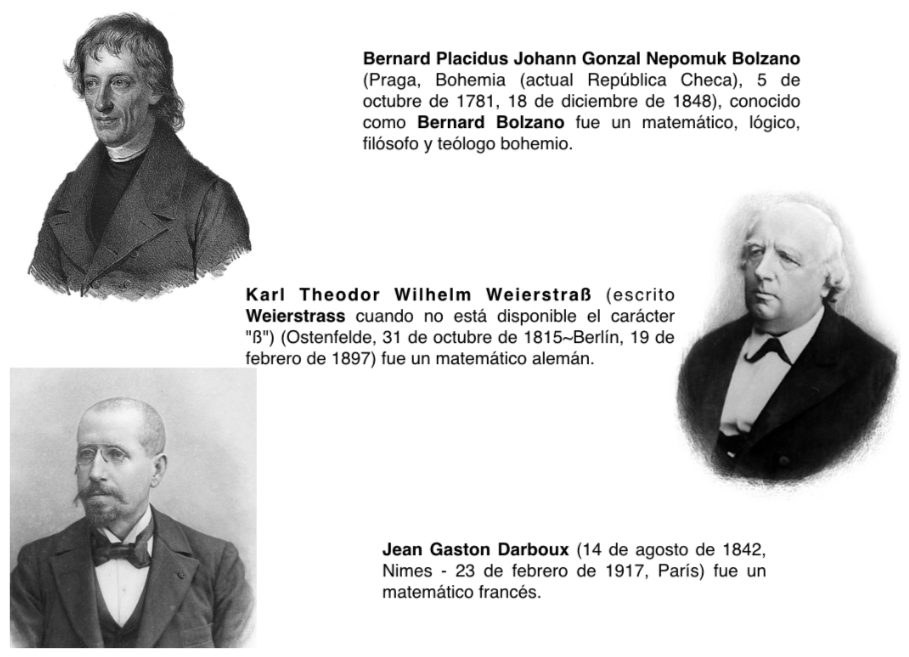
\includegraphics[width=1\textwidth]{imagenes/imagenes03/T03IM13.png}
		\end{figure}
 	
	\section{Ejercicios de teoremas de funciones continuas}
	
	\subsection{Ejercicios resueltos de teoremas de funciones continuas}
	
	
	\begin{ejre} Demuestra que la ecuación $x^3+x^2-2x$ tiene al menos una raíz en el intervalo $[1/2,3/2]$		
	\end{ejre}
	
	\begin{proofw}\renewcommand{\qedsymbol}{$\diamond$}
	
	Definimos $f(x)=x^3+x^2-2x$, que es una función continua en todo $\mathbb R$ por ser polinómica, por lo que es continua en $[1/2,3/2]$. Además, $f(1/2)=-5/8<0$ y $f(3/2)=21/8>0$. Se verifican, pues, las hipótesis del teorema de Bolzano, por lo que $\exists \; c \in [1/2,3/2] \; / \; f(c)=0$, es decir, $\exists \; c \in [1/2,3/2] \; / \; c^3+c^2-2c=0$ y es esa $c$ la raíz buscada.
	\end{proofw}
	
	
	\begin{ejre} ?`Es posible aplicar el teorema del valor intermedio en $[-2,4]$ a la función 		$f(x)=\left\{ \begin{matrix} 
		2x-1 & -2\le x <2 \\ 
		x+4 & 2 \le x \le 4  
		\end{matrix} \right.$ ?
	\end{ejre}
	
	\begin{proofw}\renewcommand{\qedsymbol}{$\diamond$}
		
	

	La función, por ser ambos trozos polimómicos, es continua en todo su dominio excepto, tal vez, en el nexo $x=2$, donde hemos de estudiar la continuidad.
	
	Continuidad en $x=2$
	
	$1)\quad \exists f(2)=2+4=6$
	
	$2)\quad \nexists \underset {x\to 2}{lim}\;{fx}$ porque no coinciden los límites laterales: $\underset{x\to 2^-}{lim}\;{2x-1}=3\neq 6 =\underset{x\to  2^+}{lim}\;{x+4}$
	
	$3) \quad $ no coinciden, f(x) es \emph{discontinua de salto} en $x=2$
	
	Al no ser $f(x)$ continua en $[-2,4]$, no se puede aplicar el teorema del valor intermedio.

	\end{proofw}
	
	\begin{ejre} Determinar si el polinomio $x^4-4x^2-1$ tiene alguna raíz negativa.		
	\end{ejre}
	
	\begin{proofw}\renewcommand{\qedsymbol}{$\diamond$}

	Hemos de encontrar un intervalo en $\mathbb R^-$ en que la función tome valores de distinto signo en sus extremos, ya que continua siempre lo será al ser un polinomio.
	
	Es fácil encontrar que en $[-3,0]$ ocurre lo dicho, $f(0)=-1<0$, $f(-3)=81-36-1=44>0$. Luego se puede aplicar el teorema de Bolzano y seguro que $\exists \; c \in ]-3,0[, \quad c<0;\quad \; / \; f(c)=c^4-4c^2-1=0$ 
	\end{proofw}
	
	\begin{ejre} Prueba que la ecuación $x=\cos x$ tiene solución positiva.		
	\end{ejre}
	
	\begin{proofw}\renewcommand{\qedsymbol}{$\diamond$}
	
	Es fácil encontrar un intervalo en $\mathbb R^+$ en que la función $f(x)=x-\cos x$, que evidentemente es continua, tome valores de distinto signo, p.e. $[0,\pi/2]$. 
	
	$f(0)=0-\cos (0)=0-1=-1<0; \quad f(\pi/2)=\pi/2-\cos(\pi/2)=\pi/2-0=\pi/2>0$. Lo cual prueba que $f(x)$ verifica el teorema de Bolzano en $[0,\pi/2]$, por lo que seguro que $\exists \; c \in ]0,\pi/2[$, es decir, $c>0$, tal que $f(c)=c-\cos(c)=0 \to c=\cos(c)$
	\end{proofw}
	
	
	\begin{ejre} 	Demuestra que existe un punto $x=c$ en el que la función $f(x)=x^2+x\cdot 2^x$ toma el valor $2$. 	
	\end{ejre}
	
	\begin{proofw}\renewcommand{\qedsymbol}{$\diamond$}
	Definimos la función $h(x)=f(x)-2=x^2+x\cdot 2^x - 2$ que es continua en todo $\mathbb R$ y al considerarla en el intervalo $[0,1]$ ocurre que toma valores de distinto signo en los extremos (compruébese) por lo que es susceptible de aplicarle el teorema de Bolzano, que demostraría la tesis que queremos probar.
	
	\end{proofw}
	
	\begin{ejre} 	$\divideontimes$. Suponiendo que la temperatura varía de forma continua, prueba que siempre hay dos puntos antípodas en el ecuador terrestre que están a la misma temperatura. 	
	\end{ejre}
	\begin{proofw}\renewcommand{\qedsymbol}{$\diamond$}
	
	Sea $L$ la longitud del ecuador terrestre (unos cuarenta mil kilómetros). Sea $T:[0,L]\to \mathbb R$	la función que a cada punto $x\in[0,L]$ le hace corresponder su temperatuta $T(x)$, medida en grados centígrados, que hay en dicho punto del ecuador. Suponemos (razonablemente) que $T(x)$ es una función continua. Se trata de probar que hay algún punto $c\in [0,L/2]$ tal que $T(c)=T(c+L/2)$ (lo de $L/2$ es por lo que los puntos han de ser antípodas). Consideremos la función $f(x)=T(x+L/2)-T(x)$, definida en el intervalo $[0,L/2]$. Se tiene que $f(0)=T(0+L/2)-T(0)=T(L/2)-T(0)$ y que $f(L/2)=T(L/2+L/2)-T(L/2)=T(L)-T(L/2)=T(0)-T(L/2)$, Ya que $L=0$, $L$ vuelve a ser el punto de partida pues el ecuador es una curva cerrada. Basta darse cuenta de que $f(0)$ y $f(L/2)$ son opuestos ($f(0)\cdot f(L/2)<0)$ y $f$ continua en $[0,L/2] \Rightarrow$ se cumple el teorema de Bolzano y $\exists \; c \in ]0,L/2[ \; / \; f(c)=0 \to T(c+L/2)-T(c)=0 \to T(c)=T(c+L/2)$, dos puntos antípodas en el ecuador que están a la misma temperatura.
	\end{proofw}

	
	\subsection{Ejercicios propuestos de teoremas de funciones continuas}
	
	
	
	\begin{enumerate}
		\item ?`Se puede asegurar que la función $f(x)=\tan x$ tiene una raíz en $[\pi/4, 3\pi/4]$ ?
		 
		\rightline{\textcolor{gris}{Solución: No, es discontinua en $\pi/2$}}
		
		\item Demuestra que existe al menos un número real que cumple: $\sin x = x-2$
		 
		\rightline{\textcolor{gris}{Solución: Bolzano a $f(x)=x-\sin x-2$ en $[0,\pi]$}}
		
		\item Demuestra que las funciones $f(x)=x\; \sin x$ y $g(x)=\ln x$ se cortan en $[2,3]$
		 
		\rightline{\textcolor{gris}{Solución: Bolzano a $h(x)=f(x)-g(x)$}}
		
		\item Demuestra que las funciones $f(x)=e^x$ y $g(x)=\dfrac 1 x$ se cortan en un $x>0$.
		 
		\rightline{\textcolor{gris}{Solución: Bolzano a $h(x)=f(x)-g(x)$ en $[0.1, 1]$}}
		
		\item ?`Se puede afirmar que $x^3+x^2-7x+1=0$ tiene al menos una solución en $]0,1[$ ? ?`Y en $]-1,0[$ ?
		 
		\rightline{\textcolor{gris}{Solución: Bolzano a $f(x)=x^3+x^2-7x+1=0$ en los intervalos indicados.}}
		\rightline{\textcolor{gris}{En el primer intervalo sí y en el segundo no}}
		
		\item Calcular, con un error menor a una décima, una raíz positiva del polinomio $x^3+x-1$
		 
		\rightline{\textcolor{gris}{Solución: Bolzano a $f(x)=x^3+x-1$ en $[0,1]$.}}
		\rightline{\textcolor{gris}{\tiny{Dividir en intervalo en 10 partes y localizar el cambio de signo.}}}
		\rightline{\textcolor{gris}{\tiny{Proceder así, dividiendo en 10 partes el intervalo en que se}}}
		\rightline{\textcolor{gris}{\tiny{ produzca el cambio de signo, hasta alcanzar la precisión deseada.}}}

		 
		\item Prueba que la función $f(x)=(x-a)^2\cdot (x-b)^2+x$ toma el valor $(a+b)/2$ para algún valor de $x$.
		 
		\rightline{\textcolor{gris}{Solución: Bolzano a $h(x)=f(x)-\dfrac {a+b}{2}$ en $[a,b]$}}
		
		
		\item Sea $f(x)=x\; \sin \left( \dfrac {\pi}{4}\; x  \right)$. Demuestra que $\exists \; \alpha\in ]0,4[: \; f(\alpha)=f(\alpha+1)$
		 
		\rightline{\textcolor{gris}{Solución: $g(x)=f(x+1); \; h(x)=g(x)-f(x), $ Bolzano en $[0,4]$}}
		
		\item La función $f(x)=\tan x\; $ toma valores de distinto signo en $[\pi/4, 3\pi/4]$ y, sin embargo, no se anula en él. ?`Contradice este ejemplo el teorema de Bolzano?
		
			\rightline{\textcolor{gris}{Solución: La función es no es continua en $[\pi/4, 3\pi/4]$, }}
			
			\rightline{\textcolor{gris}{tiene una discontinuidad asintótica en $x=\pi/2=$}}
		
		\item Demostrar que $x^5+x=1$ tiene, al menos, una solución real.
		
		\rightline{\textcolor{gris}{Solución: $f(x)=x^5+x-1$ en $[0,1]$ y Bolzano}}
		
		\item Dada $f(x)=\dfrac {4x-2}{x^2+1}$, demuestra que $\exists c \in ]0,2[\; / \; f(c)=1$
		
		\rightline{\textcolor{gris}{Solución: Considera $g(x)=f(x)-1$ en $[0,2]$ y Bolzano}}
		
		\item ?`Existe algún número real igual a su cubo menos una unidad?
		
		\rightline{\textcolor{gris}{Solución: Define $f(x)=x-(x^3-1)$, en $[0,2]$ y Bolzano}}
		
		
		\item $\divideontimes$. Un automovilista sale el sábado de Valencia a Madrid a las 8h y el domingo regresa de Madrid a Valencia a la misma hora. sabiendo que tardó el mismo tiempo en ambos viajes, prueba que en algún momento del domingo se encontraba a la misma distancia de Valencia que a la que se encontraba el sábado en ese momento.
		
		\rightline{\textcolor{gris}{ \tiny Solución: {$f(t$) distancia a Madrid el sábado, $g(t)$ distancia a Valencia el domingo definida en $[8,T]$,}}}
		\rightline{\textcolor{gris}{\tiny{ $T$ tiempo total del viaje. Aplica Bolzano a $h(t)=f(t)-(F(T)-g(t)$, con $f(T)=$ distancia Valencia-Madrid)}}}
		
		
	\end{enumerate}	
		
\chapter{La Derivada}	\label{ch-la-derivada}

	\section{Intoducción histórica}
	
	En cálculo diferencial y análisis matemático, la derivada de una función es la razón de  cambio instantánea con la que varía el valor de dicha función matemática, según se  modifique el valor de su variable independiente. La derivada de una función es un \emph{concepto local}, es decir, se calcula como el límite de la rapidez de cambio media de la función en cierto intervalo, cuando el intervalo considerado para la variable independiente se torna cada vez más pequeño. Por eso se habla del valor de la derivada de una función en un punto dado.
		
	
	Un ejemplo habitual aparece al estudiar el movimiento: si una función representa la posición de un objeto con respecto al tiempo, su derivada es la velocidad de dicho objeto para todos los momentos. Un avión que realice un vuelo transatlántico de 
$4500 km$ entre las $12:00$ y las $18:00$, viaja a una velocidad media de $750 km/h$. Sin embargo, puede estar viajando a velocidades mayores o menores en distintos tramos de la ruta. En particular, si entre las $15:00$ y las $15:30$ recorre $400 km,$ su velocidad media en ese tramo es de $800 km/h$. Para conocer su velocidad instantánea a las $15:20$, por ejemplo, es necesario calcular la velocidad media en intervalos de tiempo cada vez menores alrededor de esta hora: entre las $15:15$ y las $15:25$, entre las $15:19$ y las $15:21$.
	
El valor de la derivada de una función en un punto también puede interpretarse geométricamente, ya que se corresponde con la pendiente de la recta tangente a la gráfica de la función en dicho punto. La recta tangente es, a su vez, la gráfica de la mejor aproximación lineal de la función alrededor de dicho punto. 

\underline{Historia de la derivada}.
	
Los problemas típicos que dieron origen al cálculo infinitesimal comenzaron a plantearse en la época clásica de la antigua Grecia (siglo III a. C.), pero no se encontraron métodos sistemáticos de resolución hasta diecinueve siglos después (en el siglo XVII por obra de Isaac Newton y Gottfried Leibniz).
	
	En lo que atañe a las derivadas existen dos conceptos de tipo geométrico que le dieron origen:
	

		\hspace{5mm} * El problema de la tangente a una curva (Apolonio de Perge)
		
		\hspace{5mm} * El Teorema de los extremos: máximos y mínimos (Pierre de Fermat)
	
	En su conjunto dieron origen a lo que actualmente se conoce como cálculo diferencial.
	
	
	En el siglo XVII, los matemáticos perdieron el miedo que los griegos les habían tenido a los infinitesimales: Johannes Kepler y Bonaventura Cavalieri fueron los primeros en usarlos, empezaron a andar un camino que llevaría en medio siglo al descubrimiento del cálculo infinitesimal.
	
	A mediados del siglo XVII las cantidades infinitesimales fueron cada vez más usadas para resolver problemas de cálculos de tangentes, áreas, volúmenes; los primeros darían origen al cálculo diferencial, los otros al cálculo integral.

	A finales del siglo XVII se sintetizaron en dos conceptos los algoritmos usados por sus predecesores, en lo que hoy llamamos `derivada' e `integral'. La historia de la matemática reconoce que Isaac Newton y Gottfried Leibniz son los creadores del cálculo diferencial e integral. Ellos desarrollaron reglas para manipular las derivadas (reglas de derivación) e Isaac Barrow demostró que la derivación y la integración son operaciones inversas.
	

	Newton desarrolló en Cambridge su propio método para el cálculo de tangentes. En 1665 encontró un algoritmo para derivar funciones algebraicas que coincidía con el descubierto por Fermat. A finales de 1665 se dedicó a reestructurar las bases de su cálculo, intentando desligarse de los infinitesimales, e introdujo el concepto de \emph{fluxión}, que para él era la velocidad con la que una variable `fluye' (varía) con el tiempo.

	Gottfried Leibniz, por su parte, formuló y desarrolló el cálculo diferencial en 1675. Fue el primero en publicar los mismos resultados que Isaac Newton descubriera 10 años antes, de manera independiente. En su investigación conservó un carácter geométrico y trató a la derivada como un \emph{cociente incremental} y no como una velocidad, viendo el sentido de su correspondencia con la pendiente de la recta tangente a la curva en dicho punto.
	
	Leibniz es el inventor de diversos símbolos matemáticos. A él se deben los nombres de cálculo diferencial y cálculo integral, así como los símbolos de derivada $\; \dfrac {dy}{dx}\; $ y del símbolo integral $\int$.

	
	\section{Concepto de derivada. Interpretación geométrica y física}
	\label{IG-derivada}
	
	
	La derivada de una función puede interpretarse geométricamente como la pendiente de una curva, y físicamente como una razón `instantánea' de cambio. 
	
	\subsection{Tangente a una curva}
	 
	En la primera mitad del siglo XVII no se conocían métodos generales para calcular la tangente a una curva en un punto de la misma. Este problema se presentaba con frecuencia en mecánica, en óptica y en geometría, y generalmente se resolvía, de forma geométrica, con técnicas adaptadas a cada caso particular. La dificultad está en que, siendo la tangente una recta, se precisa conocer dos puntos de la misma, o bien un punto y su pendiente, para poderla determinar. 
	 
	 Supongamos que queremos hallar la tangente a una curva de ecuación cartesiana $y = f (x)$ en el punto $(a, f (a))$. La estrategia, usada primero por Pierre de Fermat y más tarde por Newton, consiste en aproximar la tangente por rectas secantes cuyas pendientes sí pueden calcularse directamente. En particular, consideremos la recta que une el punto $(a, f (a))$ con un punto cercano, $(x, f (x))$, de la gráfica de $f$ . Esta recta se llama una secante (recta que corta a la curva, pero no es tangente a la curva). La pendiente de esta secante es: $\dfrac {f(x) -f(a)} {x-a}$ dicho número suele llamarse \emph{cociente incremental} de $f$ en $a$. 
	 
	 \begin{multicols}{2}
	 	
	 

     
	Observa que una secante es una buena aproximación de la tangente, siempre que el punto $(x, f (x))$ esté próximo a $(a, f (a))$. Estas consideraciones llevan a definir la tangente a la gráfica de $f$ en el punto $(a, f (a))$ como la recta que pasa por dicho punto y cuya pendiente es igual al límite: $\underset{x\to a}{lim}\;{\dfrac {f(x)-f(a)}{x-a}}$ supuesto, claro está, que dicho límite exista. 
	
	 \begin{figure}[H]
			\centering
			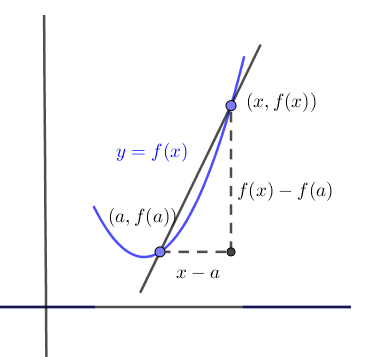
\includegraphics[width=0.4\textwidth]{imagenes/imagenes04/T04IM01.png}
			\caption {Recta secante.}
		\end{figure}
   
		\end{multicols}
		
\subsection{Razón de cambio puntual y velocidad instantánea}
	  
Muchas leyes de la Física, la Química, la Biología o la Economía, son funciones que relacionan una variable `dependiente' $y$ con otra variable `independiente' $x$, lo que suele escribirse en la forma $y = f(x)$. Si la variable independiente cambia de un valor inicial $a$ a otro $x$, la variable $y$ lo hace de $f(a)$ a $f(x)$. La razón de cambio promedio o \emph{`tasa de variación media'} de $y = f(x)$ con respecto a $x$ en el intervalo $[a, x]$ es: $\dfrac {f(x)-f(x)}{x-a}$
	  
	  Con frecuencia interesa considerar la razón de cambio en intervalos cada vez más pequeños. Esto lleva a definir lo que podemos llamar `razón de cambio instantáneo' o \emph{`tasa de variación instantánea'} de $y = f (x)$ con respecto a $x$ en el punto $a$ como: $\underset {x\to a}{lim}\;{\dfrac {f(x)-f(a)}{x-a}}$

	  El ejemplo más conocido de esto que decimos es el de un móvil que se mueve a lo largo de una recta sobre la cual hemos elegido un origen. Sea $s(t)$ la posición del móvil en el tiempo $t$, es decir, la distancia con signo del móvil al origen en el tiempo $t$. La razón de cambio promedio tiene en este caso una interpretación física natural: $\dfrac{s(a+h)-s(a)}{h}$ 
	  
	  Es la velocidad media del móvil en el intervalo de tiempo comprendido entre $a$ y $a + h$. Parece intuitivo que, en cada instante, el móvil se mueve con una determinada velocidad instantánea. Pero no hay manera de medir directamente una velocidad instantánea; un instante quiere decir una posición en la recta: la velocidad instantánea del móvil para $t = a$ es la velocidad que tiene cuando está en la posición $s(a)$. La velocidad instantánea es una abstracción de un característica física del movimiento, pero no es una magnitud que podamos observar directamente. La única definición razonable de velocidad instantánea es como la razón de cambio puntual (tasa de variación instantánea): $\underset{h\to 0}{lim}\:{\dfrac {s(a+h)-s(a)}{h}}$.
	  
	  \subsection{Definición de derivada}
	  
	  \begin{defi}
	  Se dice que $f:I\to \mathbb R$ es `devivable' en un punto $a\in I$, y se denota por $f'(a)$, si existe y es finito el límite:	
	  
	  \begin{equation}
	  	\boxed{	\quad f'(a)=\underset {x\to a}{lim}\;{\dfrac{f(x)-f(a)}{x-a}}\; \in \mathbb R \quad}
	  \end{equation}
	  
	  
	  Una notación totalmente equivalente se consigue al sustituir $x$ por $a+h$, si $x\to a$, entonces $a+h \to a$, o, lo que es lo mismo, $h\to 0$ y tenemos:
	  
	  \begin{equation}
	  		\boxed{\quad f'(a)=\underset {h\to 0}{lim}\;{\dfrac{f(a+h)-f(a)}{h}} \; \in \mathbb R \quad }
	  \end{equation}
	  
	  Esta \textbf{notación $f'(a)$} para la derivada de una función en un punto es debida a \textbf{Lagrange}. 
	  
	  Nótese que la derivada de una función en un punto es un número real.
	  \end{defi}
	  
	  $\divideontimes$ Atendiendo a la definición formal de límite vista en el capítulo anterior (definición \ref{defi:limite}), $f$ es `derivable' en $a$ si existe un número $f'(a)$ de modo que para cualquier $\varepsilon>0$, por pequeño que sea, somos capaces de encontrar un $\delta>0$ tal que para todo $x\in I, \; x\neq a$ y con $|x-a|<\delta$ se cumple que $\left|\dfrac {f(x)-f(a)}{x-a} - f'(a) \right|<\varepsilon$
	  
	  
	  \section{Función derivada}
	  
	  \begin{defi}
	  Sea $f:I\to \mathbb R$, derivable en todo punto de $I$. Llamamos función derivada de $f$ y la representamos por $f'$ a la función: $f':I\to \mathbb R$ tal que a cada punto $x\in I$ le hace corresponder su derivada en ese punto, $f'(x)$.	
	  \end{defi}
	  
	  \subsection{Otras notaciones para las derivadas}
	  
	   \begin{multicols}{2}
	   $\quad$
	   
	  Aparte de la \textbf{notación de Lagrange: $f'(x)$} que acabamos de ver, hay otras notaciones para las derivadas.
	  	\begin{figure}[H]
			\centering
			\includegraphics[width=0.5\textwidth]{imagenes/imagenes04/xiste04.png}
			\label{mates-fisics}
		\end{figure}
		\end{multicols}
	
	\vspace{-5mm}
	
	  Notación de \textbf{diferencial de Leibniz, $\dfrac {\dd f(x)}{\dd x} $}. Se lee derivada de $f(x)$ respecto de $x$. Esta notación tiene la ventaja de sugerir la derivada como cociente de elementos infinitesimales (diferenciales) y es muy usada en física. Veremos su enorme utilidad práctica y enorme sencillez cuando estudiemos la derivada de las funciones compuestas y la derivada de la función inversa.
	  
	
	  Con esta notación, la derivada de una función en un punto se representa como:  $\eval{ \dfrac {\dd f(x)}{\dd x} }_{x=a} $, o también como $\left( \dfrac {\dd f(x)}{\dd x}  \right)\; (a)$
	  
	  
	  
	  
	  Notación de \textbf{Newton: $ \dot { y }=y' $}. Esta notación, aunque incómoda, sigue utilizándose en mecánica para referirse a la derivada temporal de una variable:  $\dot {x}= \dfrac {\dd x(t)}{\dd t}=x'(t)$

	  
	Notación de \textbf{Euler: $D_x \; f=f'(x)$}
	
	\subsection{Rectas Tangente y Normal a una función en un punto. Elementos de una curva relacionados con la derivada}
	 \label{subsec:RTN} 
	  
	  \begin{defi}Recta tangente a una curva. Supuesto $f$ derivable en $a$, la ecuación:
	  
	  \begin{equation}
	  	\boxed{\; y-f(a)=f'(a)\cdot(x-a) \; }
	  	\label{eq:recta-tangente}
	  \end{equation}
	  	
	  	Es la ecuación de la recta tangente a $f(x)$ en el punto $(a,f(a))$
	  \end{defi}
	  
	  \begin{defi}Recta Normal a una curva. Supuesto $f$ derivable en $a$, con $f'(a)\neq 0$, la ecuación:
	  
	  \begin{equation}
	  	\boxed{ \; y-f(a)=-\dfrac 1 {f'(a)}\cdot(x-a) \; }
	  	\label{eq:recta-normal}
	  \end{equation}
	  	
	  	Es la ecuación de la recta normal (perpendicular) a $f(x)$ en el punto $(a,f(a))$
	  \end{defi}
	  
	  
	   $\divideontimes$ \textbf{Elementos de una curva relacionados con la derivada.}
	  
	 \begin{figure}[H]
		\centering
		\includegraphics[width=0.5\textwidth]{imagenes/imagenes04/T04IM02.png}
		\caption {Elementos de una curva relacionados con la derivada.}
	\end{figure}
	
	\begin{itemize}
		\item La pendiente de la recta tangente (la que pasa por los puntos VP) es $\tan \theta = y'$.
		\item La pendiente de la recta normal (la que pasa por los puntos UN) es $\tan \alpha = \tan (\pi/2 + \alpha)=-1/y'$.
		\item El segmento $\overline {TM}$ es la \textbf{subtangente}. Su longitud viene dada por $\overline  {TM}=y \; \cot( \theta ) = y/y'$ 
		\item El segmento $\overline{MN}$ es la \textbf{subnormal}. Su longitud viene dada por $\overline{MN}=y\; \tan(\theta)=yy'$.	
		\item Los segmentos interceptados por los ejes $OX$ y $OY$ con la tangente son:
		
		
		\begin{equation*}
		\begin{cases}
		\overline{OT}=\overline{OM}-\overline{TM}=x-y/y'  \\ 
		\overline{OV}=\overline{PM}-\overline{PQ}=y-x\; \tan(\theta)=y-xy'   
		\end{cases}
		\end{equation*}
		
		
		\item Los segmentos interceptados por los ejes $OX$ y $OY$ con la normal son:
		
		\begin{equation*}
		\begin{cases}
			\overline{ON}=\overline{OM}+\overline{MN}=x+y\; \tan (\theta)=x+yy'  \\ 
			\overline{OU}
			=\overline{OH}+\overline{HU}=y+x\; \tan (\phi)=y+x\; \tan (\pi/2 - \theta)=y+x/y' 
		\end{cases}
		\end{equation*}
		
	%\begin{equation*}
	%\begin{pmatrix*}[l]
	%\overline{OT}=\overline{OM}-\overline{TM}=x-y/y'  \\ 
	%\overline{OV}=\overline{PM}-\overline{PQ}=y-x\; \tan(\theta)=y-xy' 
	%\end{pmatrix*}
	%\end{equation*}
		
		
		\end{itemize}
	
	
	 \begin{figure}[H]
			\centering
			\includegraphics[width=0.9\textwidth]{imagenes/imagenes04/T04IM07.png}
			\caption {Recuerda la interpretación de derivada.}
			\label{img:mantra-derivada}
	\end{figure}
	
	
	
	\section{Derivadas laterales}
	
	\begin{defi} Derivadas laterales.
	
	Decimos que \textbf{$f$ es derivable por la izquierda en $a$}, y lo representamos por $f'_{-}(a)$ (análogamente \textbf{ $f$derivable por la derecha en $a$}, $f'_{+}(a)$) si existen y son finitos los límites:
	
		\begin{equation}
		\label{ref:derivada-lateral}
			f'_{-}(a)=\underset{x\to a^-}{lim}\;{\dfrac {f(x)-f(a)}{x-a}} \qquad ; \qquad f'_{+}(a)=\underset{x\to a^+}{lim}\;{\dfrac {f(x)-f(a)}{x-a}}
		\end{equation}
		
		Analogamente:
		\begin{equation}
			f'_{-}(a)=\underset{h\to 0^-}{lim}\;{\dfrac {f(a+h)-f(a)}{h}} \qquad ; \qquad f'_{+}(a)=\underset{h\to 0^+}{lim}\;{\dfrac {f(a+h)-f(a)}{h}}
		\end{equation}
		
		
		Teniendo en cuenta la relación entre límites y límites laterales, está claro que una función es derivable en un punto si existen, son finitas y coinciden sus derivadas laterales.
		
		\begin{equation}
			\exists f'(a) \leftrightarrow \exists f'_-(a), \; \exists f'_+(a) \; \wedge \; f'_-(a)=f`_+(a)
		\end{equation}
		
	\end{defi}
	
	\begin{multicols}{2}
		
	Cuando en una función $f$ continua en un punto $a$ las derivadas laterales existen, son finitas, pero distintas, decimos que en $a$ la función tiene un 	\emph{Punto Anguloso}, hay no una sino dos rectas tangentes distintas a la izquierda y a la derecha de $a$. Así como intuitivamente una función es continua en un punto si se puede dibujar, en un entorno de ese punto, sin `levantar el lápiz del papel', una función será derivable si \underline{además} el comportamiento en un entorno de ese punto es \emph{suave}, no abrupto, como aparece el la imagen de al lado.
	
	\begin{figure}[H]
		\centering
		\includegraphics[width=0.3\textwidth]{imagenes/imagenes04/T04IM03.png}
		\caption {Punto anguloso.}
	\end{figure}
	
	\end{multicols}
	
	
	\section{Relación entre continuidad y derivabilidad}
	
	
	El siguiente teorema demuestra que la condición de derivabilidad es más fuerte o restrictiva que la de continuidad.
	
	\begin{teor}
	\label{teor:deriv-cont}
		Todo función derivable en un punto, es continua en él.
	\end{teor}

	\begin{proof}
		Sea $f:I\to \mathbb R$, derivable en $a$, es decir, $\exists f'(a)=\underset{x\to a}{lim}\;{\dfrac {f(x)-f(a)}{x-a}} \in \mathbb R$
		
		Consideremos la igualdad: $f(x)=f(a)+(x-a) \cdot \dfrac {f(x)-f(a)}{x-a} \qquad x\in I; \; x\neq a $, tomando límites cuando $x\to a$ se deduce que:
		
		$\underset {x\to a}{lim }{f(x)}= \underset {x\to a}{lim }{ f(a)+{(x-a)} \cdot \dfrac {f(x)-f(a)}{(x-a)} }=f(a)+\cancelto {0}{(x-a)} \cdot f'(a)= f(a)$, lo que indica que f(x) es continua en $a$.
		
	\end{proof}
	
	Obviamente, si una función no es continua en en punto no se podrá trazar una recta tangente en él, por lo que será no-derivable. Pero el hecho de que sea continua no asegura que sea derivable.
	
	El recíproco del teorema anterior no se cumple, no todas las funciones continuas son derivables, sirva como contraejemplo la figura anterior o, incluso, la función valor absoluto.
	
	
		\begin{figure}[H]
			\centering
			\includegraphics[width=0.8\textwidth]{imagenes/imagenes04/T04IM06.png}
			\caption{Funciones continuas y no derivables.}
		\end{figure}
		
		\begin{figure}[H]
			\centering
			\includegraphics[width=0.6\textwidth]{imagenes/imagenes04/T04IM08.png}
			\caption{Verde: no continua en cero; Roja: continua en cero, pero no derivable; azul: continua y derivable en cero.}
			\label{fig:ctndaddvbdad}
		\end{figure}
		
		
	
	\begin{ejem} Calcular la derivada de la función $f(x)=|x|$ en el punto $a=0$
		
	\begin{multicols}{2}
		

	$f'(0)=\underset{h\to 0}{lim}\;{\dfrac {f(0+h)-f(0)} {h}}=\underset {h\to 0}{lim}\; {\dfrac {f(h)}{h}}$. Es necesario estudiar límites laterales (derivadas laterales) pues $0$ es el nexo de la función a trozos valor absoluto de $x$.
	
	$f'_-(0)=\underset{h\to 0^-}{lim}\;{\dfrac {-h}{h}}=-1 \qquad f'_+(0)=\underset{h\to 0^+}{lim}\;{\dfrac {+h}{h}}=+1$
	
	Como $f'_-(0)=-1\neq 1=f'_+(0) \to \nexists f'(0)$, la función no es derivable en el $0$, aunque sí continua, por lo que en $0$ la función presenta un punto anguloso.
	
	\begin{figure}[H]
			\centering
			\includegraphics[width=0.4\textwidth]{imagenes/imagenes04/T04IM04.png}
			\caption{Función Valor Absoluto.}
		\end{figure}
		
	\end{multicols}
	
	\end{ejem}
	
	\begin{ejem} Usando la definición de derivada, calcula las rectas tangente y normal a $f(x)=2x^2+3x+1$ en el punto $a=-1 \qquad $\scriptsize{\textcolor{gris}{$f'(x)=4x+3 \to f'(-1)=4(-1)+3=-1$}}
	
	\normalsize
	Usemos una de las dos definiciones:
	
	$f('-1)=\underset {x\to -1}{lim}\;{\dfrac {f(x)-f(-1)}{x-(-1)}}= \underset {x\to -1}{lim}\;{\dfrac {2x^2+3x+1-0}{x+1}}=$
	
	$\underset {x\to -1}{lim}\;{\dfrac {2x^2+3x+1}{x+1}}=[0/0; \; ind]= \underset {x\to -1}{lim}\;{\dfrac {\cancel{(x+1)}(2x+1)}{\cancel{(x+1)}}}=$
	
	$\underset {x\to -1}{lim}\;{(2x+1)=2(-1)+1=-1}$
	
	Usando la otra definición:
	
	$f'(-1)=\underset {h\to 0}{lim}\; {\dfrac {f(-1+h)-f(-1)} {h}}= \underset {h\to 0}{lim}\; {\dfrac {2(-1+h)^2+3(-1+h)+1-0} {h}}=$
	
	$=\underset {h\to 0}{lim}\; {\dfrac {2(-1+h)^2+3(-1+h)+1-0} {h}}= \underset {h\to 0}{lim}\; {\dfrac {2h^2-h} {h}}=[0/0;\; ind]=$
	
	$ = \underset {h\to 0}{lim}\; {\dfrac {\cancel{h}(2h-1} {\cancel{h}}}=\underset {h\to 0}{lim}\; {(2 \cancelto{0}{h} - 1)}=-1$
	
	En cada caso, una de las dos definiciones es más útil que la otra.
	
	Puesto que tanto la recta tangente como la normal pasan por el punto $(-1,f(-1))=(-1,0)$ y teniendo en cuenta las ecuaciones de ambas rectas, ecuación \ref{eq:recta-tangente} y ecuación \ref{eq:recta-normal}, tenemos:
	
	Recta tangente a $f(x)$ en $x=-1 \quad \to \quad y-0=-1(x-(-1)); \quad y=-x-1$
	
	Recta normal a $f(x)$ en $x=-1 \quad \to \quad y-0=-\dfrac {1}{-1}(x-(-1)); \quad y=x+1$
	
	\end{ejem}
	
	\begin{ejem}  $\divideontimes$
	
	Dada la función $f(x)=\frac 1 2 x^2-2x+3$, calcula	$f'(4)$, las rectas tangente y normal en $x=4$ y los segmentos subtangente y subnormal.
	
	Es fácil comprobar que $f'(4)=2$, que la recta tangente es $y=2x-5$ y la recta normal $y=-\frac 1 2 x +5$. El segmento subtangente mide $6$ y el subnormal $1.5$
	
		\begin{figure}[H]
			\centering
			\includegraphics[width=0.7\textwidth]{imagenes/imagenes04/T04IM05.png}
			\caption{Subtangente y subnormal.}
		\end{figure}
	
	\end{ejem}
	
	\begin{ejem} Aplicando la definición de derivada, calcula $f'(2)$ a la función: $f(x)=\dfrac {2x}{x-1}$.
	
	$f'(2)=\underset {h\to 0}{lim}\;{\dfrac {f(2+h)-f(2)}{h}}= \underset {h\to 0}{lim}\;{\dfrac { \dfrac{2(2+h)}{(2+h)-1}-4}{h}} = \underset {h\to 0}{lim}\;{\dfrac {\dfrac {4+2h}{h+1}-4}{h}}=\underset {h\to 0}{lim}\;{\dfrac {4+2h-4(h+1)}{h(h+1)}}=\underset {h\to 0}{lim}\;{\dfrac {-2 \cancel{h}}{\cancel{h}(h+1)}}=\dfrac {-2}{1}=-2$
		
	\end{ejem}
	
	\begin{ejem} Calcula, aplicando la definición de derivada, $f'(4)$ para $f(x)=\sqrt{2x+1}$
	
	$f'(4)=\underset {x \to 4}{lim}\; {\dfrac {f(x)-f(4)}{x-4}}= \underset {x \to 4}{lim}\; {\dfrac {\sqrt{2x+1}-3}{x-4}}=[0/0\; ind]= $
	
	$\underset {x \to 4}{lim}\; {\left( \dfrac {\sqrt{2x+1}-3}{x-4}\cdot \dfrac {\sqrt{2x+1}+3}{\sqrt{2x+1}+3} \right) } = \underset {x \to 4}{lim}\; {\dfrac {2x+1-9}{(x-4)\cdot(\sqrt{2x+1}+3) }} = $
	
	$\underset {x \to 4}{lim}\; {\dfrac {2\cancel{(x-4)}}{\cancel{(x-4)}\cdot(\sqrt{2x+1}+3) }}= \underset {x \to 4}{lim}\; {\dfrac {2}{\sqrt{2x+1}+3 }}=\dfrac {2}{3+3}=\dfrac 2 6 =\dfrac 1 3$
		
	\end{ejem}
	
	\begin{ejem} Para la siguiente función, comprueba que en $x=1$ es continua, pero no derivable.
	
	\begin{equation*}
		f(x)=
		\begin{cases} 
		\;\;  3x-2 &\mbox{ si } x\le 1 \\ 
		\; x^2 & \mbox{ si } x>1 
		\end{cases}
	\end{equation*}
	
	Continuidad en x=1 (método de los tres pasos):
	
	$1) \quad \exists f(1)=3(1)-2=1$
	
	$2) \quad \exists \underset{x\to 1^-}{lim}\;{3x-2}=1=\underset{x\to 1^+}{lim}\;{x^2}=\underset{x\to 1}{lim}\;{f(x)}$
	
	$3) \quad $ Coinciden. Luego $f(x)$ continua en $x=1$
	
	Estudiemos ahora la derivabilidad en $x=1$:
	
	$1) \quad \exists f'_-(1)=\underset {x\to 1^-}{lim}\;{\dfrac {f(x)-f(1)}{x-1}}=\underset {x\to 1^-}{lim}\;{\dfrac {3x-2-1}{x-1}}=\underset {x\to 1^-}{lim}\;{\dfrac {3\cancel{(x-1)}}{\cancel{(x-1)}}}=3$
	
	$2) \quad \exists f'_+(1)=\underset {x\to 1^+}{lim}\;{\dfrac {f(x)-f(1)}{x-1}}= \underset {x\to 1^+}{lim}\;{\dfrac {x^2-1}{x-1}}=\underset {x\to 1^+}{lim}\;{\dfrac {(x+1)\cancel{(x-1)}}{\cancel{(x-1)}}}=2$
	
	$3) \quad f'_-(1)=3\neq 2=f'_+(1) \to \nexists f'(1)$ y la función es no derivable en $x=1$
	
	Tenemos una función que en $x=1$ es continua pero no derivable porque las derivadas laterales existen ambas, son finitas, pero distintas. Decimos que en $x=1$ la función $f(x)$ tiene un \emph{punto anguloso.}
	\end{ejem}
	
	\section{Álgebra de derivadas}
	
	\begin{teor}Álgebra de derivadas
	\label{teor:algebra-derivadas}
	
	Sean $f$ y $g$ dos funciones derivables en un cierto intervalo $I$ y sea $x\in I$, sea $k\in \mathbb R$, entonces se cumplen las siguientes reglas de derivación:
	
	\begin{itemize}
		\item $(k\cdot f)'(x)=k\cdot f'(x)$
		
		Derivada de constante por función: la constante no se deriva y se multiplica por la derivada de la función.
		
		\item $(f+g)'(x)=f'(x)+g'(x)$
		
		Derivada de la suma es igual a la suma de derivadas.
		
		\item $(f-g)'(x)=f'(x)-g'(x)$
		
		Derivada de la resta es igual a la resta de derivadas.
		
		\item $(f\cdot g)'(x)=f'(x)\cdot g(x)+f(x)\cdot g'(x)$
		
		Derivada del producto es igual a la derivada de la primera función por la segunda sin derivar, más la primera sin derivar por la derivada de la segunda función.
		
		\item $\left( \dfrac f g \right)'(x)=\dfrac {f'(x)\cdot g(x) - f(x)\cdot g'(x)}{g^2(x)}$
		
		Derivada del cociente es igual a la derivada del numerador por el denominador sin derivar, \underline{menos} el numerador sin derivar por la derivada del denominador; todo ello dividido por el denominador al cuadrado.

	\end{itemize}
	
			
	\end{teor}
	
	\begin{proof}
		
		$\divideontimes$  Demostraremos alguna de ellas:
		
		Derivada de la suma:
		
		$(f+g)'(x)=\underset {h\to 0}{lim}\;{\dfrac {(f+g)(x+h)-(f+g)(x)}{h}}=$
		
		$\underset {h\to 0}{lim}\;{\dfrac {f(x+h)+g(x+h)-(f(x)+g(x))}{h}}$
		
		$=\underset {h\to 0}{lim}\;{\left\{\dfrac {f(x+h)-f(x)}{h}+\dfrac {g(x+h)-g(x)}{h}\right\}}=\underset {h\to 0}{lim}\;{\dfrac {f(x+h)-f(x)}{h}}+ \underset {h\to 0}{lim}\;{\dfrac {g(x+h)-g(x)}{h}}=f'(x)+g'(x)$
		
		Derivada del cociente:
		
		$\left( \dfrac f g \right)'(x)=\underset{h\to 0}{lim}\;
		{ \dfrac { \left(\dfrac{f}{g}\right)(x+h)-\left(\dfrac{f}{g}\right)(x)   }{h}}= \underset {h\to 0}{lim}\;{\dfrac { \dfrac {f(x+h)}{g(x+h)} - \dfrac{f(x)}{g(x)} }{h}}=$
		
		$ =\underset {h\to 0}{lim}\; {\dfrac {f(x+h)g(x)-f(x)g(x+h) }{h g(x+h)g(x)}}= $
		
		$\underset {h\to 0}{lim}\; {\dfrac {f(x+h)g(x) \textbf{-f(x)g(x)+f(x)g(x)}-f(x)g(x+h) }{h \; g(x+h)\; g(x)}}=$
		
		$=\underset {h\to 0}{lim};{\dfrac {1}{g(x+h)g(x)} \cdot \left[ \dfrac {f(x+h)-f(x)}{h}\cdot g(x) - f(x)\cdot \dfrac {g(x+h)-g(x)}{h} \right]}=$
		
		$=\dfrac {1}{g^2(x)}[f'(x)g(x)-f(x)g'(x)]$
		
		
	\end{proof}
	
	\section{Derivadas de las funciones elementales}
	
	Demostraremos solo algunas de ellas.
	
	\begin{teor} Derivadas funciones elementales.
		
		\begin{itemize}
			\item $f(x)=k \to f'(x)=0$
			\item $f(x)=x \to f'(x)=1$
			\item $f(x)=x^n \to f'(x)=n\cdot x^{n-1}$
			\item $f(x)=a^x \to f'(x)=\ln a \cdot a^x; \quad f(x)=e^x \to f'(x)=e^x$
			\item $f(x)=\log_a x \to f'(x)=\dfrac {1}{\ln a \cdot x}; \quad f(x)=\ln x \to f'(x)=\dfrac 1 x$
			\item $f(x)=\sin x \to f'(x)=\cos x$
			\item $f(x)=\cos x \to f'(x)=-\sin x$
			\item $f(x)=\tan x =\dfrac {\sin x}{\cos x}\to f'(x)=1+\tan^2 x= \dfrac {1}{\cos^2 x}$
			\item etc. Ya ampliaremos todo esto en una tabla de derivadas.
		\end{itemize}
		
	\end{teor}

	\begin{proof}   $\divideontimes$ Demostraremos solo algunas de ellas.
	
	Derivada de la función identidad:
	
	$f(x)=x \to f'(x)=\underset{h\to 0}{lim}\;{\dfrac {f(x+h)-f(x)}{h}}=\underset {h \to 0}{lim}\;{\dfrac {x+h-x}{h}}=\underset{h\to 0}{lim}\;{1}=1$
	
	\vspace{4mm}Derivada de la función potencial:
	
	$f(x)=x^n \to f'(x)=\underset {h\to 0}{lim}\;{\dfrac {f(x+h)-f(x)}{h}}=\underset{h\to 0}{lim}\;{\dfrac {(x+h)^n - x^n}{h}}=$
	
	Teniendo en cuenta la fórmula del binomio de Newton demostrada en el ejercicio resuelto \ref{ejre:binomio-newton}:
	
	\noindent \footnotesize{$= \underset {h\to 0}{lim}\;{\dfrac { \cancel{\left( \begin{matrix} n \\ 0 \end{matrix} \right) x^n} + \left( \begin{matrix} n \\ 1 \end{matrix} \right) x^{n-1}\; h + \left( \begin{matrix} n \\ 2 \end{matrix} \right) x^{n-2} h^2 + ... + \left( \begin{matrix} n \\ n-1 \end{matrix} \right) x h^{n-1} + \left( \begin{matrix} n \\ n \end{matrix} \right) h^n \; -\; \cancel{x^n}   }{h}}=$}
	
	\noindent  $=\underset{h\to 0}{lim}\;{\dfrac {\cancel{h}\cdot \left[\left( \begin{matrix} n \\ 1 \end{matrix} \right) x^{n-1)} + \left( \begin{matrix} n \\ 2 \end{matrix} \right) x^{n-2} \cancelto{0}{h} + \left( \begin{matrix} n \\ 3 \end{matrix} \right) x^{n-3}\cancelto{0}{h^2} + ... + \left( \begin{matrix} n \\ n \end{matrix} \right) \cancelto{0}{h^{n-1}}   \right]}{\cancel{h}}} $\normalsize{$=$}
	
	$ = \left( \begin{matrix} n \\ 1 \end{matrix} \right) x^{n-1}= \dfrac {n!}{1!\cdot (n-1)!}x^{n-1}=n\; x^{n-1}$
	
	\vspace{4mm}Derivada de la función seno:
	
	$f(x)=\sin x \to f'(x)=\underset{h\to 0}{lim}\;{\dfrac {\sin(x+h)-\sin x}{h}}=  $
	
	$\underset{h\to 0}{lim}\;{\dfrac {(\cancel{\sin x} \; \cancelto{1}{\cos h} \; + \; \cos x\; \sin h)-\cancel{\sin x}}{h}}=$

	Teniendo en cuenta que $\underset {h\to 0}{lim}{\dfrac {\sin h}{h}}=1$ tal y como vimos en el ejemplo \ref{ejem:sinx/x}, tenemos que:	
	
	$=\underset{h\to 0}{lim}\;{\cos x \; \cancelto{1}{ \dfrac {\sin h}{h}} }=\cos x$
		
	\end{proof}
	
	
		\section{Ejercicios elementales de derivadas}
	
	Aunque estos ejercicios ya deben saberse del curso anterior, haremos y propondremos algunos como repaso.
	
	\subsection{Ejercicios resueltos de derivadas simples}
	
	
	\begin{ejre} Deriva las siguientes funciones:
	
	\begin{multicols}{2}
	
	\begin{enumerate}
		\item $f(x)=\sqrt x$
		\item $f(x)=\dfrac 1 x$
		\item $f(x)=\cot x$
		\item $f(x)=7x^3-4x^2-3x+5$
		\item $f(x)=\dfrac {3x-1}{5x^2-4}$
		\item $f(x)=e^x\cdot \sin x$
		\item $f(x)=\sqrt{x}\; e^x\; \cos x$
		\item $f(x)=\dfrac {\sin x + \cos x}{\sin x - \cos x}$
	\end{enumerate}
		
	\end{multicols}

		
	\end{ejre}
	
	
	
	\begin{proofw}\renewcommand{\qedsymbol}{$\diamond$}
	
	Resolvamos:
		
		\begin{enumerate}
			\item $y=\sqrt{x}=x^{\frac 1 2} \to y'=\frac 1 2 x^{\frac 1 2 - 1}= \frac 1 2 x^{-\frac 1 2}= \dfrac {1}{2 \sqrt {x}}$. 
			
			Como la raíz cuadrada es tan común en ciencia, vale la pena recordar su derivada. $y=\sqrt{x} \to y'=\dfrac {1}{2 \sqrt {x}}$
			\item $y=\dfrac 1 x = x^{-1}\to y'=-1\; x^{-1-1}=-1 x^{-2}=-\dfrac 1 {x^2}$
			
			Como en el caso anterior, al ser la inversa muy común también es conveniente recordar su derivada: $y=\dfrac 1 x \to y'=-\dfrac 1 {x^2}$
			
			\item $y=\cot x=\dfrac {\cos x}{\sin x} \to y'=\dfrac {(\cos x)'\cdot (\sin x) - (\cos x)\cdot (\sin x)' }{\sin^2 x}$
			
			$=\dfrac {-\sin^2 x - \cos^2 x}{\sin^2 x}= \dfrac {-1}{\sin^2 x}$
			
			\item $y=7x^3-4x^2-3x+5 \to y'=21x^2-8x-3$
			
			\item $y=\dfrac {3x-1}{5x^2-4} \to y'=\dfrac {3(5x^2-4)-(3x-1)10x}{(5x^2-4)^2}=\dfrac {-15x^2+10x-12}{(5x^2-4)^2}$
			
			\item $y=e^x \; \sin x \to y'= e^x \; \sin x +e^x \; \cos x=e^x\; (\sin x + \cos x) $
			
			\item $y=\sqrt{x} \; e^x \cos x = \sqrt{x} \; (e^x \cos x) \to y'= \dfrac {1}{2 \sqrt{x}}\cdot (e^x \cos x) + \sqrt{x} \cdot (e^x \cos x)' = \dfrac {1}{2 \sqrt{x}}\cdot (e^x \cos x) + \sqrt{x} \cdot (e^x \cos x + e^x (-\sin x)) = \dfrac {1}{2 \sqrt{x}}\cdot (e^x \cos x) + \sqrt{x} \cdot (e^x \cos x - e^x \sin x)$
			
			\item $y=\dfrac {\sin x + \cos x}{\sin x - \cos x} \to $
			
			$y'=\dfrac {(\cos x - \sin x)(\sin x - \cos x)-(\sin x + \cos x)(\cos x + \sin x)}{(\sin x - \cos x)^2}=$
			
			$\dfrac {-2}{(\sin x - \cos x)^2}$
			
		\end{enumerate}
		
	\end{proofw}

	
	
	\subsection{Ejercicios propuestos de derivadas simples}
	
	\begin{enumerate}
		\item $y=-\dfrac {x^3+x-1}{2} \qquad $ \textcolor{gris}{$\to \quad y'=-\frac 3 2 x^2-\frac 1 2$}
		\item $y=- \frac 2 {x^3}+ \frac 3 {x^2}-4x \qquad$ \textcolor{gris}{$\to \quad y'=\frac 6 {x^4}-\frac 6 {x^3}-4$}
		\item $y=\dfrac {5x^4-3x^3}{x^5} \qquad$ \textcolor{gris}{$\to \quad y'=-\frac 5 {x^2}+\frac 6 {x^3}$}
		\item $y=\sqrt{x^3} \qquad$ \textcolor{gris}{$\to \quad y'=\frac 3 2 \sqrt{x}$}
		\item $y=-3 \sqrt{x}-2 \sqrt[3]{x^2} \qquad$ \textcolor{gris}{$\to \quad y'= \dfrac{-3}{2\sqrt{x}}-\dfrac{4}{3\sqrt[3]{x}}$}
		\item $y=\dfrac{\sqrt{x}\; \sqrt[3]{x}}{\sqrt[4]{x}} \qquad $ \textcolor{gris}{$\to \quad y'=\dfrac {7}{12\; \sqrt[12]{x^5}}$}
		\item $y=\dfrac{e^x \; \sin x}{x^2 \; \ln x} \qquad$ \textcolor{gris}{$\to \quad y'= \dfrac {x^2 \ln x \; e^x (\sin x +\cos x)- e^x \sin x (2x \ln x + x)}{x^4 \ln^2 x}$ }
		
	\end{enumerate}
	
	\section{Derivada de la función compuesta: `Regla de la cadena'}
	
		\begin{teor} Regla de la Cadena.
	\label{teor:regla-cadena}	
	
	Sea $f:]a,b[\to \mathbb R$ y $g:]c,d[\to \mathbb R$ , con $Rec(f) \subset ]c,d[ \quad \to \quad (g\circ f)(x)=g(f(x))$
	
	Conocidos $f'(x)$ y $g'(x)$, se trata de encontrar $(g\circ f)'(x)$.
	
	Esta relación se conoce como la `derivada de la función compuesta' o `regla de la cadena' y es de enorme utilidad en el cálculo de derivadas.
	
	Demostraremos que, en las condiciones anteriores, se cumple que:
	
	\begin{equation}
		(g\circ f)'(x)=g'\left( f(x)\right) \cdot f'(x)
	\end{equation}
	
	\end{teor}
	
	\begin{proof}Calculemos $(g\circ f)'(x)$ aplicando la definición de derivada:
	
	$(g\circ f)'(x)=\underset {h \to 0}{lim}\; {\dfrac {(g \circ f)(x+h)-(g\circ f)(x)}{h}}=\underset {h \to 0}{lim}\; {\dfrac {g\left(f(x+h)\right)-g\left(f(x)\right)}{h}}$
	
	$=\underset {h \to 0}{lim}\; { \dfrac {g\left(f(x+h)\right)-g\left(f(x)\right )}{f(x+h)-f(x)} \cdot \dfrac {f(x+h)-f(x)}{h}  }= g'(f(x))\cdot f'(x)$
		
	\end{proof}
	
	La \emph{regla de la cadena} puede aplicarse a la composición de más de dos funciones:
	
	
	$(h\circ g \circ f)'(x)= h'((g\circ f)(x))\cdot (g \circ f)'(x)=h'(g(f(x))\cdot g'(f(x))\cdot f'(x)$
	
	\begin{ejem} Sea $f(x)=5x+2; \quad g(x)=x^2.\qquad \mbox{Calcular } (g\circ f)'(x)$
	
	$(g\circ f)(x)=g(f(x))=g(5x+2)=(5x+2)^2$
	
	$(g \circ f)'(x)=g'(f(x))\; f'(x)$
	
	$g(x)=x^2 \to g'(x)=2x; \qquad g'(5x+2)=2\cdot (5x+2)$
	
	$f(x)=5x+2 \to f'(x)=5$
	
	$(g\circ f)'(x)= 2\cdot (5x+2) \cdot 5 = 10(5x+2)=50x+20$
	
	\textcolor{gris}{Cosa que, en este caso podemos comprobar (no así en el siguiente ejemplo) ya que $(g\circ f)(x)=(5x+2)^2=25x^2+20x+4 \quad \to \quad (g\circ f)'(x)=50x+20$}
		
	\end{ejem}
	
	\begin{ejem} Deriva la función $y=\sin(3x^2-1)$
	
	Si nos acostumbramos a usar la notación $y=\sin(u)$, cuando $u$ sea a su vez una función de $x$, podemos decir que $y'=(\cos u) \cdot u'$, con ello:
	
	$y'=(\cos(3x^2-1))  \cdot  (6x)$, que escribiremos más cómodamente, para evitar confusiones, como: $y'=6x \; \cos (3x^2-1)$
		
	\end{ejem} 
	
	
	\begin{ejem} Derivar $y=\ln(\sin x)$ usando la notación de Leibniz.
	
	Puesto que $\sin x \neq x \to \sin x=u$, con lo cual hemos de derivar $y=\ln u$, siendo $u=\sin x$.
	
	En notación de Leibniz: $\dfrac {\dd y}{\dd x}= \dfrac {\dd y}{\dd u} \cdot \dfrac {\dd u }{\dd x}= \dfrac 1 u \cdot \cos x= \dfrac 1 {\sin x}\; \cos x= \cot x$	
	\end{ejem}

	Algunas veces ayuda pensar en la regla de la cadena de esta manera: si $y=g(f(x)) \to y'=\dfrac {\dd y}{\dd x}=g'(f(x))\cdot f'(x)$. Es decir, derivar la función más externa $g'$ y evaluarla en la función interna $f$ y, después, multiplicar por la derivada de la función más interna $f'$, podríamos decir que consiste en derivar `de fuera hacia adentro'.
	
	\begin{ejem} Deriva la función $y=e^{\sin (3x^2-1)}$
	
	Derivando de fuera hacia adentro, tendremos: $y'=e^{\sin (3x^2-1)}\cdot \cos(3x^2-1) \cdot 6x$, que, reordenando quedará como: $ y'=6x \; \cos(3x^2-1) \; e^{\sin (3x^2-1)}$	
	\end{ejem}
	
	\section{Derivación implícita. Derivación logarítmica}
	
	DERIVACIÓN IMPLÍCITA: Vamos a ver cómo derivar una expresión implícita, en que la variable independiente no está despejada (función explícita). Supongamos $y=f(x)$, entonces, si se tiene una expresión del tipo:
	
	$g(x)+a_ny^n+a_{n-1}y^{n-1}+ \dots + a_1y+a_0=0$
	
	Teniendo en cuenta que $(y^n)'=(f^n(x))'=nf^{n-1}(x)\; f'(x)=n\; y^{n-1}\; y'$
	
	Tendríamos, derivando: $g'(x)+n a_n y^{n-1}\; y' +\dots +a_1\; y' =0$
	
	Y, despejando $y'=\dfrac {-g'(x)}{n\; a_n\; y^{n-1} + \dots + a_1}$
	
	\begin{ejem} Deriva la función $x^2+y^2=4$ \textcolor{gris}{(ecuación de una circunferencia de radio 2 centrada en el origen de coordenadas)}.
	
	$2x+2y\cdot y'=0 \to 2y\; y'=-2x \to y'=-x/y$	
	\end{ejem}

	Aunque en este ejemplo hubiésemos podido despejar $y$ y derivar explícitamente, no siempre es posible hacerlo. Veamos el siguiente ejemplo:
	
	\begin{ejem} Deriva $e^{xy}+3x^2y^3=\sen(x+y)$
	
	$e^{xy}\cdot (y+xy')+ 6 x y^3 + 3x^2 \cdot 3y^2\; y' = (\cos(x+y))(1+y') $ y, de ahí, despejar $y'$.
	
	$e^{xy}xy'+9x^2y^2y'-\cos(x+y)y'=\cos(x+y)-e^{xy}y - 6xy^3$
	
	$y'=\dfrac{\cos(x+y)-e^{xy}y - 6xy^3}{e^{xy}x+9x^2y^2-\cos(x+y)}$ 
	
	Para la derivación implícita es conveniente recordar que así como $(x)'=1; \; (y)'=y'$
	\end{ejem}
	
	DERIVACIÓN LOGARÍTMICA: La derivada de la función logarítmica, la regla de la cadena y la derivación implícita nos proporcionan un método de derivación extraordinariamente útil en el caso de grandes productos cocientes y potencias $\left( \dfrac {(3x^2-1)^7 \cdot \tan^3 x}{\sqrt[7]{sin^5 x}\cdot e^{\sin x}} \right)$, así como en las funciones que no son ni potenciales ($x^k,\; k=cte$) ni exponenciales ($k^x$), algunos autores les llaman funciones potenciales-exponenciales. Nos referimos a funciones del tipo $f(x)^{g(x)}$ como, por ejemplo $x^x$ o $(\sin x)^{\tan x}$, es decir, funciones expresadas por potencias en que tanto base como exponente son, a su vez, funciones de $x$.
	
	Los pasos a seguir en el caso de la aplicación de la derivación logarítmica son:
	
	\begin{enumerate}
		\item Tomar logaritmos en la expresión a derivar y aplicar sus propiedades.
		\item Derivar implícitamente
		\item Despejar y'
	\end{enumerate}
	
	\begin{ejem} Deriva la función $y=x^x$ (*)
	
	$1) \quad \ln y = \ln x^x = x \cdot \ln x$
	
	$2) \quad y'/y= 1 \; \ln x + x \; \frac 1 x = (\ln x + 1)$
	
	$3) \quad y'=(\ln x + 1) \cdot y=(\ln x + 1)\; x^x$ (*)
		
	\end{ejem}
	
	\begin{ejem} Deriva $y=(\sin x)^{\tan x}$
	
	$1) \quad \ln y= \tan x \; \ln (\sin x)$
	
	$2) \quad y'/y= \dfrac 1 {\cos^2 x}\; \ln (\sin x) + \tan x\; \dfrac {\cos x}{\sin x} = \dfrac {\ln (\sin x)}{\cos^2 x} + 1$
	
	$3) \quad y'= \left( \dfrac {\ln (\sin x)}{\cos^2 x} + 1 \right) \; (\sin x)^{\tan x}$
		
	\end{ejem}
	
	\begin{ejem} Deriva la función: $y=\dfrac {(3x^2-1)^7 \cdot \tan^3 x}{\sqrt[7]{sin^5 x}\cdot e^{\sin x}}$
	
	
	$1) \quad \ln y= 7 \ln (3x^2-1) + 3 \ln (\tan x) - \frac 5 7 \ln (sin x) - \sin x$
	
	$2) \quad y'/y= 7 \dfrac {6x}{3x^2-1} + 3 \dfrac {1 + \tan^2 x}{\tan x} - \frac 5 7 \dfrac {\cos x}{\sin x}- \cos x$
	
	$3) \quad y'= \left(  \dfrac {42x}{3x^2-1} +  \dfrac {3(1 + \tan^2 x)}{\tan x} - \frac 5 7 \cot x- \cos x  \right) \cdot \dfrac {(3x^2-1)^7 \cdot \tan^3 x}{\sqrt[7]{sin^5 x}\cdot e^{\sin x}}$
		
	\end{ejem}

	Los dos primeros ejemplos de derivación logarítmica no se pueden hacer de otro modo, el tercer ejemplo se puede derivar como un cociente pero piénsese en la complejidad del mismo. La derivación logarítmica es imprescindible cuando tenemos funciones del tipo $f(x)^{g(x)}$ pero muy útil en otros casos (productos , cocientes y potencias que el logaritmo rompe fácilmente en sumas y restas)
	
	
	\section{Derivada de la función Inversa}
	
	\begin{teor} Derivada de la función inversa.
	
	
	
	Sean $I, \; J$ dos intervalos abiertos, $y=f(x):I \to J$ una función biyectiva (En matemáticas, una función es biyectiva si es al mismo tiempo inyectiva y sobreyectiva; es decir, si todos los elementos del conjunto de salida tienen una imagen distinta en el conjunto de llegada, y a cada elemento del conjunto de llegada le corresponde un elemento del conjunto de salida.)
		
		Si $f'(x)\neq 0,\; \forall x \in I \Rightarrow (f^{-1})'(x)=\dfrac {1} {f' \left(  f^{-1}(x) \right)} $
	\end{teor}
	
	\begin{proof}Para la demostración del teorema de la función inversa conviene recordar la propiedad vista en la proposición \ref{prop:funcion-inversa}:  $(f\circ f^{-1})(x)=x$
	
	Sin más que aplicar la regla de la cadena, tenemos:
	
	$(f\circ f^{-1})'(x)=f'(f^{-1}(x))\cdot (f^{-1})'(x)=1\to (f^{-1})'(x)= \dfrac {1} {f' \left(  f^{-1}(x) \right)}$
		
	\end{proof}

	
	\begin{ejem} Derivar la función $y=\arctan x$
	
	$y=\arctan x \to x=\tan y \Rightarrow (\arctan)'(x)=\dfrac {1}{(\tan)'(y)}=\dfrac {1}{1+ \tan^2 y}=\dfrac {1}{1+x^2}$
		
	\end{ejem}
	
	La notación de Leibniz simplifica enormemente la derivada de la función inversa:  $\dfrac {\dd y}{\dd x}= \dfrac {1}{\dfrac {\dd x}{\dd y}}$ Según esto, el ejemplo anterior se convierte en:
	
	$y=\arctan x \leftrightarrow x=\tan y \Rightarrow$
	
	$(\arctan)'(x)=\dfrac {\dd y}{\dd x}= \frac {\dd }{\dd x} (\arctan x) = \dfrac {1}{\dfrac {\dd (tan y)}{\dd y}}= \dfrac {1}{1+\tan^2 y}=\dfrac {1}{1+x^2}$
	
	
	\begin{ejem} Calcula la derivada de $y=\arccsc x$ (arccsc es el arco cosecante).
	
	$y=\arccsc x \leftrightarrow x=\csc y = \dfrac 1 {\sin y} \to \sin y= \dfrac 1 x$ (*)
	
	$y'=(\arccsc x)'=\dfrac {\dd y}{\dd x}= \dfrac {1}{\dfrac {\dd x}{\dd y}}= \dfrac {1}{-\dfrac {1}{\sin^2 y}\; \cos y}=-\dfrac {\sin^2 y}{\cos y}= -\dfrac {\sin^2 y}{\sqrt{1-\sin^2 y}}= -\dfrac {\dfrac {1}{x^2}}{\sqrt{1-\dfrac {1}{x^2}}}=-\dfrac {1}{x\sqrt{x^2-1}} $
		
	\end{ejem}
	
	\begin{ejem} $\divideontimes$ Calcula la derivada de $y=\mathrm{arg\;sinh}\; x$ (Visto en la subsección \ref{subsec:func-hiperb})
	
	Es fácil comprobar que si $y=\sinh x \to y'=\cosh x$. Se deja como ejercicio al lector.
	
	El $\mathrm{arg\;sinh}\; x$ es la función inversa del $\sinh x$, por ello: $y=\mathrm{arg\;sinh}\; x \to x=\sinh y$
	
	$\dfrac {\dd y}{\dd x}= \dfrac {1}{\dfrac {\dd x}{\dd y} }= \dfrac 1 {\cosh y} \Rightarrow$ [Recordando la relación entre las funciones hiperbólicas: $\cosh^2 x - \sinh^2 x=1 \to \cosh y=\sqrt{\sinh^2 y + 1}$  $\Rightarrow (\mathrm{arg\;sinh}\; x)'\dfrac {1}{\sqrt{\sinh^2 y + 1}}=\dfrac {1}{\sqrt{x^2+1}}$
	\end{ejem}
	
	\section{Tabla de derivadas}
	
	Em el apéndice \ref{app:tabla-derivadas} aparece una tabla más completa de las derivadas de las funciones elementales.
	
	ALGEBRA DE DERIVADAS:
		
		$(k\cdot f)'=k\cdot f' \; \quad (f\pm g)'=f' \pm g'\ ;  \quad (f\cdot g)'=f'\cdot g + f\cdot g' \ ; \quad \left({\dfrac f g}\right) '=\dfrac {f'\cdot g - f\cdot g'}{g^2}$
		
		\vspace{5mm}
		
		REGLA DE LA CADENA:  $\left({g\left (f(x) \right)}\right)' = g'\left(f(x) \right) \cdot f'(x)$
		
		\vspace{5mm}
		

		TABLA DE DERIVADAS:
		
		
		 \begin{table}[hbt]
		  \centering
		   \begin{tabular}{|l|l||l|l|}
		   \hline
		  $f(x)$ & $f'(x)$ & $f(x)$ & $f'(x)$\\[5pt] \hline \hline
		   $k$ & $0$ & $x$ & $1$\\ \hline
		   $x^n$ & $n\ x^{n-1}$ & $u^n$ & $n\ u^{n-1}\ \textbf {u'}$\\ \hline
		   $\sqrt{x}$ & $\dfrac {1}{2 \sqrt{x}}$ & $\sqrt{u}$ & $\dfrac {1}{2\ \sqrt{u}}\ \textbf {u'}$\\[10pt] \hline
		   $e^x \ || \quad a^x$ & $e^x \ || \quad a^x\ \ln a$ & $e^u\ || \quad a^u$ & $e^u \ \textbf {u'}\ || \quad a^u\ \ln a\ \textbf {u'}$\\ \hline
		   
		   $\ln x\ || \quad \log_a x$ & $\dfrac {1} {x}\ || \quad \dfrac {1}{x \ \ln a}$ & $\ln u\ || \quad \log_a u$ & $\dfrac {1}{u}\ \textbf {u'}\ || \quad \dfrac {1}{u\ \ln a}\ \textbf {u'}$\\[10pt] \hline
		   $\sin x$ & $\cos x$ & $\sin u$ & $\cos u\ \textbf {u'}$ \\ \hline
		   $\cos x$ & $-\sin x$ & $\cos u$ & $-\sin u\ \textbf {u'}$ \\ \hline
		   $\tan x$ & $\dfrac {1}{\cos^2 x}=1+\tan^2 x$ & $\tan u$ &  \footnotesize{$\dfrac {1}{\cos^2 u} \ \textbf {u'} = (1+\tan^2 u)\ \textbf {u'}$}\\[10pt] \hline
		   $\arcsin x$ & $\dfrac {1}{\sqrt{1-x^2}}$ & $\arcsin u$ & $\dfrac {1}{\sqrt{1-u^2}}\ \textbf {u'}$ \\[10pt] \hline
		   $\arccos x$ & $\dfrac {-1}{\sqrt{1-x^2}}$ & $\arccos u$ & $\dfrac {-1}{\sqrt{1-u^2}}\ \textbf {u'}$ \\[10pt] \hline
		   \vspace{2mm}
		   $\arctan x$ & $\dfrac {1}{1+x^2}$ & $\arctan u$ & $\dfrac {1}{1+u^2}\ \textbf {u'}$ \\ \hline
		  \end{tabular}
		\end{table}
		
	
	\vspace {10mm}
	
	DERIVADA FUNCIÓN INVERSA:   
	
	$(f^{-1})'(x)=\dfrac 1 {f'(f^{-1}(x))};\ \quad Leibniz: \dfrac {dy}{dx}=\dfrac {1}{\dfrac {dx}{dy}}$
	
	\vspace {5mm}
	
	DERIVACIÓN IMPLÍCITA:  Para funciones implícitas:$\phi(x,y)$. Tener en cuenta que $(y)'=y'$
	
	\vspace {5mm}
	
	DERIVACIÓN LOGARÍTMICA: Para funciones del tipo $(f(x))^{g(x)}$, tomar logaritmos en la expresión y derivar implícitamente.

\section{Derivadas de funciones a trozos}
	
	Para derivar una función definida a trozos (perdiendo un poco el rigor, puesto que en lo siguiente supondremos que $f'$ sea continua y no tiene por qué serlo) se deriva en los trozos \textit{abiertos} (desigualdades estrictas) y, previo estudio de la continuidad, se mira si las derivadas laterales coinciden en los nexos (si esto no ocurre, estaremos ante \textit{puntos angulosos}). Es evidente (teorema \ref{teor:deriv-cont}) que si una función no es continua, no será derivable.
	
	\begin{ejem} Deriva la función:
	
	\hspace{20mm}  $y=
	\begin{cases}
		x^2 & \mbox{ si } x\le 1 \\
		2x-1 & \mbox{ si } 1<x<3 \\
		4-x & \mbox{ si } 3\le x \le 4 \\
		x-4 & \mbox{ si } x>4
	\end{cases} .$
	
	Estudiando previamente la continuidad de $f(x)$ en los nexos $\{1,3,4 \}$ pues en en resto de números reales la función es continua, pues todos sus trozos son polinomios, haciendo el estudio riguroso de los tres pasos en cada uno de los puntos de estudio (se deja como ejercicio para el lector), se obtiene que: $f_-(1)=1=f_+(1)$, continua en $x=1$; $f-(3)=5\neq 1=f_+(3)$, función discontinua de salto en $x=3$, por lo que $\nexists f'(3)$ y $f-(4)=0=f_+(4)$, función continua en $x=4$.
	
	Obtengamos ahora la función $y'=f'(x)$ derivando solo en los intervalos abiertos (desigualdades estrictas):
	
		\hspace{20mm} $y'=f'(x)=
	\begin{cases}
		2x & \mbox{ si } x< 1 \\
		2 & \mbox{ si } 1<x<3 \\
		-1 & \mbox{ si } 3< x <4 \\
		1 & \mbox{ si } x>4
	\end{cases} .$
	
	Veamos, ahora, las derivadas laterales en los nexos:
	
	$f'_-(1)=\underset{x\to 1^-}{lim}\;{f(x)}=\underset{x\to 1^-}{lim}\;{2x}=2\cdot 1=2; \qquad f'_+(1)=\underset{x\to 1^+}{lim}\;{f(x)}=\underset{x\to 1^+}{lim}\;{2}=2 \quad \Rightarrow \quad f_-(1)=f_+(1)=2 \quad \to \quad \exists f'(1)=2$
	
	Al ser $f$ discontinua en $x=3 \quad \nexists f'(3)$
	
	$f'_-(4)=\underset{x\to 4^-}{lim}\;{f(x)}=\underset{x\to 4^-}{lim}\;{-1}=-1; \qquad f'_+(4)=\underset{x\to 4^+}{lim}\;{f(x)}=\underset{x\to 4^+}{lim}\;{1}=1 \quad \Rightarrow \quad f_-(4)=-1\neq 1=f_+(4) \quad \to \quad \nexists f'(4)$, en $x=4$ la función es continua pero no derivable (derivadas laterales finitas y distintas), en $x=4$ hay un Punto Anguloso.
		
	\end{ejem}
\section{Derivadas sucesivas   $\; \divideontimes$    }
\label{derivadas-sucesivas}
	
	Si $f'$ es derivable, podemos construir $(f')'=f''$ que llamaremos función \textit{derivada segunda}. Así, sucesivamente, podemos hablar de $f''', f^{iv}, f^{v},\;  ... \; f^{n)}$ \textbf{Derivadas sucesivas}.
	
	\begin{ejem} Calcula la derivada enésima de la función $y=\ln x$
	
	$y=\ln x \to y'=\dfrac 1 x = x^{-1} \to y''=(-1)x^{-2} \to y'''=(-1)(-2)x^{-3} \to  y^{iv}=(-1)(-2)(-3)x^{-4} \to \dots \to y^{n)}=(-1)^{n-1}(n-1)!\; x^{-n}=\dfrac{(-1)^{n-1}(n-1)!}{x^n}$
	
	Esta conjetura a la que hemos llegado, para ser rigurosos, necesitaría una demostración por el método de inducción.
		
	\end{ejem}
	
	\begin{ejem} Calcula la derivada enésima de $y=\sin x$
	
	$y=\sin x \to y'=\cos x \to y''=-\sin x \to y'''=-\cos x \to y^{iv}=\sin x =y$ y, a partir de ahí se repite cada 4 veces. 
	

	
	Una forma elegante de escribir esto es recordar la fórmula trigonométrica $y=\cos x=\sin (x+\frac \pi 2)$
	
		$y=\sin x \to y'=\cos x=\sin (x+\frac \pi 2) \to y''=\cos (x+\frac \pi 2)=\sin (x+\frac \pi 2+ \frac \pi 2)=\sin (x+2\frac \pi 2) \to y'''=\sin (x+3\frac \pi 2) \to \dots \to y^{n)}=\sin (x+n\frac \pi 2)$
	
	\end{ejem}
	
	\begin{ejem} 
	Obviamente, si $y=e^x \to y^{n)}=e^x$ 
		
	\end{ejem}
	
	 \emph{Fórmula de LEIBNIZ para la derivada enésima de un producto}. Damos esta fórmula por su belleza matemática que, obviamente, tiene que ver con la fórmula del binomio de Newton: $\; \divideontimes$
	
	\begin{equation}
	\footnotesize{
		(f\cdot g)^{n)}=
		\left( \begin{matrix} n \\ 0 \end{matrix} \right) 
		f^{n)} \; g + 
		\left( \begin{matrix} n \\ 1 \end{matrix} \right)
		f^{n-1)}\; g' + 
		\left( \begin{matrix} n \\ 2 \end{matrix} \right) 
		f^{n-2)}\; g'' 
		+ \dots + 
		\left( \begin{matrix} n \\ n-a \end{matrix} \right)  
		f'\; g^{n-1)}+ 
		\left( \begin{matrix} n \\ n \end{matrix} \right) 
		f \; g^{n)} 
		}
	\end{equation}
	
	\subsection{Otras notaciones para derivadas enésimas $\; \divideontimes$ }
	
	\begin{itemize}
		\item \normalsize{Lagrange}: $y'; \quad y''; \quad y'''\; \quad \cdots$
		\item Leibniz: $\dfrac {\dd y}{\dd x}; \quad \dfrac {\dd^2 y}{\dd x^2}; \quad \dfrac {\dd^3 y}{\dd x^3}; \quad \cdots$ 
		
		Que se leen: derivada de y respecto de x; derivada segunda de y respecto de x dos veces, derivada tercera de y respecto de x tres veces, ...
		\item Newton: $\dot { y } ;\quad \ddot { y } ;\quad \dddot { y } ;\quad \cdots $
		\item Euler: $D\; y; \quad D_2\; y; \quad D_3\; y; \quad \cdots$ 
	\end{itemize}
	
	
	
	\section{La diferencial}
	%\vspace{-10mm}
				\begin{multicols}{2}
					
				

				
				$f$ dvble. en $I$, $x_0 \in I$, se define la  \textbf{diferencial de f en $x_0$ con incremento $h$} como:
				
	
				$df_h (x_0)=f'(x_0)\cdot h=f'(x_0)\cdot \Delta x$
				
			
				$df_h (x_0)$ es una aprox. de $\Delta f_h (x_0)$:
				
				$\Delta f_h(x_0)= f(x_0+h)-f(x_0) \simeq$
				
				$\simeq f'(x_0)\cdot h = f'(x_0)\cdot \Delta x = df_h(x_0)$
				
			
				Despejando: 
				
				$\boxed {\; f(x_0+h)\simeq f(x_0)+f'(x_0)\cdot h \; }$ 
				
			
		\begin{figure}[H]
			\centering
			\includegraphics[width=0.40\textwidth]{imagenes/imagenes04/T04IM13.png}
			\caption {La Diferencial.}
		\end{figure}
			
		\end{multicols}	
		
		
		Estamos aproximando el valor de una función en un punto de difícil cálculo, $f(x_0+h)$, por el valor de esa función en un punto cercano y fácil de calcular, $f(x_0)$, y un término lineal (polinomio de primer grado) en $h$, $f'(x_0)\cdot h$. Esta aproximación será mejor cuanto menor sea $h$ y es \textit{la primera aproximación de una función}: en vez de considerar el crecimiento de la función $f(x_0+h)$, tomamos lo que crece su recta tangente $f(x_0)+f'(x_0)\cdot h$. Tomando derivadas de orden superior se encuentran polinomios de mayor grado que proporcionan mejores aproximaciones, son los desarrollos en serie de Taylor que veremos en futuros capítulos..
		
	
	
		En la práctica se usa:  $h=\Delta x= dx$ que se llama \textit{diferencial de x} (una cantidad muy pequeña -infinitesimal- en notación de Leibniz). Así: $df(x)=f'(x)\cdot dx = \dfrac {\dd f(x)}{\dd x}\dd x$
		
		\begin{ejem} Calcula un valor aproximado de $\sqrt{15.8}$
		
		Consideremos la función $f(x)=\sqrt{x}$, que es fácil calcular en el punto $x_0=16$, pero que es difícil calcular en el punto $x_0+h=15.8\to h=-0.2$. Como $f(x_0)=f(16)=\sqrt{16}=4; $ y $\; f'(x)=\dfrac {1}{2\sqrt{x}}\to f'(x_0)=f'(16)=\dfrac {1}{2\sqrt{16}}=\dfrac 1 8$, tendremos:
		
		$f(x_0+h)\simeq f(x_0)+f'(x_0)\cdot h$ 
		
		$f(16-0.2)=f(15.8)=\sqrt{15.8}\simeq f(16)+f'(16)\cdot (-0.2)=4+\dfrac 1 8 (-0.2)=4-0.025=3.975 \qquad $  \textcolor{gris}{El verdadero valor es $\sqrt{15.8}=3,974921382870358$}
			
		\end{ejem}
		
		\begin{ejem} Calcula $\dd (\ln \sqrt{1-\sin x})$
		
		$\dd y = f'(x) \dd x \to \dd (\ln \sqrt{1-\sin x})= \dfrac {1}{\sqrt{1-\sin x}} \dfrac {1}{2\sqrt{1-\sin x}}(-\cos x)\; \dd x=\dfrac {\cos x}{2(\sin x - 1)} \dd x$	
			
		
					
		\end{ejem}
		
		\begin{ejem} Las dimensiones de un cilindro son $5 \; dm$ de altura y $2 \; dm$ de radio. Calcula un valor aproximado de la variación que experimenta el volumen del cilindro si, manteniéndose constante la altura, el radio aumente en un $3 \%$
		
		El volumen del cilindro viene dado por la expresión $V=\pi r^2 \; h$. Si suponemos que la $h$ se mantiene constante, tenemos $V(r)=\pi r^2 \; h$. Al pasar el radio del valor $r=2\; dm$ al valor $r+\dd r=2+ 0.03\cdot 2=2.06 \; dm$, el volumen experimentará un cambio $\Delta V=V(r+\dd r)-V(r)$, pero estamos buscando una aproximación con la diferencial:
		
		$\Delta V \approx \dd  V =  \pi \; 2 r \; \dd r\; h= 2 \pi h r \dd r = 2 \pi \; 5 \cdot 2 \cdot 0.06 \approx 3.77 \; dm^3$ 
		\end{ejem}
		
			\section{Ejercicios de derivadas}
	\subsection{Ejercicios resueltos de derivadas}
	
	\begin{ejre} Utilizando la definición de derivada, calcula $f'(2)$ para los siguientes casos:
	
	$a) \quad f(x)=\dfrac {x-1}{x+1}; \qquad b) \quad f(x)=\sqrt{x+2}$
	\end{ejre}
	
	\begin{proofw}\renewcommand{\qedsymbol}{$\diamond$}
	
	$a) \quad f'(2)=\underset{x\to 2}{lim}\;{\dfrac {f(x)-f(2)}{x-2}}= \underset{x\to 2}{lim}\; {\dfrac {\dfrac {x-1}{x+1}-\dfrac 1 3}{x-2}}=\underset{x\to 2}{lim}\; {\dfrac {3(x-1)-(x+1)}{3(x+1)(x-2)}}=\underset{x\to 2}{lim}\; {\dfrac {2\cancel{(x-2)}}{3(x+1)\cancel{(x-2)}}}=\dfrac 2 9$
	
	$b) \quad f'(2)=\underset{h\to 0}{lim}\;{\dfrac {f(2+h)-f(2)}{h}}=\underset{h\to 0}{lim}\;{\dfrac {\sqrt{h+4}-2}{h}}=[0/0;\mbox{ ind }]= \underset{h\to 0}{lim}\;{\dfrac {\sqrt{h+4}-2}{h}}\cdot \dfrac {\sqrt{h+4}+2}{\sqrt{h+4}+2}=\underset{h\to 0}{lim}\;{\dfrac {\cancel{h}}{\cancel{h}\cdot(\sqrt{h+4}+2) }}=\dfrac 1 4$
	
	\end{proofw}
	
	\begin{ejre} Determina la diferencial para cada una de las siguientes funciones: $f(x)=x^4-2x^2+1;\quad g(x)=e^{2x^2+1}$	
	\end{ejre}
	
	\begin{proofw}\renewcommand{\qedsymbol}{$\diamond$}
	
	$\dd f= (4x^3-4x)\; \dd x \qquad \dd g= 4x\; e^{2x^2+1}\; \dd x$
	\end{proofw}
	
	\begin{ejre} Calcula un valor aproximado de las expresiones: 
	
	$\quad \dfrac 1 {4.001}; \quad \dfrac {1}{2,01^3}$	
	\end{ejre}
	
	\begin{proofw}\renewcommand{\qedsymbol}{$\diamond$}
	
	$\dfrac 1 {4.001} \to f(x)=\dfrac 1 x;\quad x_0+h=4.001;\quad h=0.001; \quad x_0=4; \quad f'(x)=-\dfrac 1 {x^2}$
	
	$f(x_0+h) \approx f(x_0)+f'(x_0) \cdot h \Rightarrow \dfrac 1 {4.001} \approx 0.25 + (-0.0625)\cdot 0.01 \approx 0.24994$
	
	$\quad$
	
	$\dfrac {1}{2,01^3} \to f(x)=\dfrac 1 {x^3};\quad x_0+h=2.01;\quad h=0.01; \quad x_0=2; \quad f'(x)=-\dfrac 3 {x^4}$
	
	$f(x_0+h) \approx f(x_0)+f'(x_0) \cdot h \Rightarrow \dfrac 1 {2,01^3} \approx 0.125 + (-0.1875)\cdot 0.01 \approx 0.12313$
	\end{proofw}

	\begin{ejre} 	Comprueba que la siguiente función es continua y derivable. Calcula $f'(0);\; f'(1);\; f'(3)$. Calcula $f'(x)$ y comprueba si hay algún punto en que $f'(x)=5$
	
			$f(x)=
		\begin{cases}
		3x-1 & \mbox{ si } x< 1 \\
		x^2+x & \mbox{ si } x\ge 1  
		\end{cases} ;$
	\end{ejre}
	
	\begin{proofw}\renewcommand{\qedsymbol}{$\diamond$}
	
	Continuidad de $f(x)$ en $x=1$, en el resto siempre continua (polinomios):
	
	$1) \quad \exists f(1)=1^2+1=2$
	
	$2) \quad \exists \underset{x\to 1^-}{lim}\;{3x-1}=2=\underset{x\to 1^+}{lim}\;{x^2+x}=\underset{x\to 1}{lim}\;{f(x)}$
	
	$3) \quad $Coinciden, luego $f(x)$ es continua en $x=1$. Para ver si es derivable estudiaremos si coinciden sus derivadas laterales a partir de $f'(x)$.
	
	Calculemos, ahora, $f'(x)$ derivando solo en los intervalos abiertos:
	
	$f'(x)=
		\begin{cases}
		3 & \mbox{ si } x< 1 \\
		2x+1 & \mbox{ si } x >1  
		\end{cases} ; \qquad \mbox{?`} \exists f'(1)?$
		
		$f'_-(1)=\underset{x\to 1^-}{lim}\;{f'(x)}=\underset{x\to 1^-}{lim}\;{3}=3$
		
		$f'_+(1)=\underset{x\to 1^+}{lim}\;{f'(x)}=\underset{x\to 1^+}{lim}\;{2x+1}=3$
		
		Como $f'_-(1)=3=f'_+(1) \Rightarrow \exists f'(1)=3$. Muchos autores reescriben la función derivada incluyendo este último resultado, $f'(1)=3$, por ejemplo así:
		
			$f'(x)=
		\begin{cases}
		3 & \mbox{ si } x\le 1 \\
		2x+1 & \mbox{ si } x >1  
		\end{cases} $
		
		Contestemos ahora a las restantes preguntas $f'(0)= 3;\quad f'(1)=3;\quad  f'(3)=7$
		
		Probemos, por último, si $\exists x \; / \;  f'(x)=5$
		
		$\mbox{si }x\le 1 \to f'(x)=3 \neq 5$. Para $x\le 1$ la ecuación propuesta $f'(x)=5$ no tiene solución.
		
		$\mbox{si }x> 1 \to f'(x)=2x+1 =5 \leftrightarrow x=2 \in ]1,+\infty[$. Para $x> 1$ la ecuación propuesta $f'(x)=5$ sí tiene solución, $x=2$.
		
	
	\end{proofw}
	
	\begin{ejre} 	Calcula los valores de $m$ y $n$ para que $f$ sea derivable en todo $\mathbb R$ 
	
		$f(x)=
		\begin{cases}
		x^2-5x+m & \mbox{ si } x\le 1 \\
		-x^2+nx & \mbox{ si } x >1  
		\end{cases} $
		
		?`En qué puntos es $f'(x)=0$?
	\end{ejre}
	
	\begin{proof}[]
	\renewcommand{\qedsymbol}{$\diamond$}
	
	Por ser una función a trozos, ambos polinómicos, $f(x)$ es continua en todo $\mathbb R$ excepto, tal vez, en el nexo $x=1$ donde estudiamos la continuidad con el método de los tres pasos:
	
	$1) \quad \exists f(1)=1^2-5+m=-4+m$
	
	$2) \quad \exists \underset{x\to 1^-}{lim}\;{x^2-5x+m}=-4+m$
	$ \exists \underset{x\to 1^+}{lim}\;{-x^2+nx}=-1+n$
	Para que $\exists \underset{x\to 1}{lim}\;{f(x)}$, los límites laterales han de coincidir, por lo que: $-4+m=-1+n \to m-n=3 \quad (1*)$
	
	$3) \quad$ Coinciden siempre que se cumpla la condición $(1*)$ y $f(x)$ será continua en $x=1$ y, probablemente derivable.
	
	Estudiemos fa función derivada:
	
	$f'(x)=
		\begin{cases}
		2x-5 & \mbox{ si } x< 1 \\
		-2x+n & \mbox{ si } x >1  
		\end{cases} ; \qquad \mbox{?`} \exists f'(1)?$
		
	$f'_-(1)=2-5=-3; f'_+(1)=-2+n \Rightarrow $ Para que $\exists f'(1)$, las derivadas laterales debe coincidir, por lo que exigimos que $-3=-2+n \to n=-1 \quad (2*)$
	
	De las condiciones exigidas $(1*)$ y $(2*)$ tenemos un sistema de dos ecuaciones con dos incógnitas cuya solución es:
	
	$\begin{cases}
		m-n=3 \\
		n=-1
	\end{cases}  \qquad \Rightarrow \qquad m=2 \; \wedge \; n=-1$
	
	Recopilando, escribimos ahora $f'(x)$ como queda y estudiaremos si $f'(x)=0$ tiene solución.
	
	$f'(x)=
		\begin{cases}
		2x-5 & \mbox{ si } x\le 1 \\
		-2x-1 & \mbox{ si } x >1  
		\end{cases}$
	
	Para $x\le 1 :\; f'(x)=2x-5=0 \mbox{ si } x=\dfrac 5 2 = 2.5 \notin ]-\infty,1[ $. No hay solución.
	
	Para $x> 1 : \; f'(x)=-2x-1=0 \mbox{ si } x=-\dfrac 1 2 = -0.5 \notin ]1,+\infty[ $. No hay solución.
	
	Luego, $\nexists x \; / \; f'(x)=0$. Esta función no tiene puntos de derivada nula.
	\end{proof}
	
\begin{ejre} Calcula $f'$ y $f''$ para la función:
	
	$f(x)=x\cdot |x|=
	\begin{cases}
		-x^2 & \mbox { si } x<0 \\
		x^2  & \mbox { si } x\ge 0
	\end{cases}$	
	\end{ejre}
	
	\begin{proofw}\renewcommand{\qedsymbol}{$\diamond$}
	La función es continua en todo $\mathbb R$ excepto, tal vez, en $x=0$ por ser nexo. Pero, abreviando: $f-(0)=0=f_+(0)=f(0)$, continua en $x=0$, continua en todo $\mathbb R$.
	
	$f'(x)=
		\begin{cases}
		-2x & \mbox{ si } x< 0 \\
		2x & \mbox{ si } x >0  
		\end{cases} ; \qquad  \exists f'(0)=f'_-(0)=f'_+(0)=0$
		
		La función derivada $f'$ también es continua en todo $\mathbb R$:
		
	$f'(x)=
		\begin{cases}
		-2x & \mbox{ si } x< 0 \\
		2x & \mbox{ si } x \ge0  
		\end{cases}$	
		
		Calculemos la derivada segunda:
		
	$f''(x)=
		\begin{cases}
		-2 & \mbox{ si } x< 0 \\
		2 & \mbox{ si } x >0  
		\end{cases} ; \qquad   f''_-(0)=-2 \neq f''_+(0)=2 \to \nexists f''(0)$	
		
		Es decir:
		
		$f''(x)=
		\begin{cases}
		-2 & \mbox{ si } x< 0 \\
		2 & \mbox{ si } x >0  
		\end{cases}$
		
		Conclusión: $f'$ es continua en todo $\mathbb R$, pero $f''$ solo es continua en $\mathbb R \sim \{0\}$
	
	\end{proofw}
	
	\begin{ejre} 	Estudia la derivabilidad de la función 
	$f(x)=\dfrac 1 {1+|x|}$
	\end{ejre}
	
	\begin{proofw}\renewcommand{\qedsymbol}{$\diamond$}
	
	$f(x)=\dfrac 1 {1+|x|}=
	\begin{cases}
		\dfrac 1 {1-x} & \mbox{ si } x<0 \\
		\dfrac 1 {1+x} & \mbox{ si } x\ge0
	\end{cases}$
	
	Función continua en todo $\mathbb R$ por que sus denominadores no se anulan nunca ($1-x\neq 0, \; x<1$ y $1+x\neq 0, \; x\ge1$). Además, $f_-(0)=1=f_+(0)=f(0)$, la función es continua en el $0$.
	
	Calculemos la función derivada:
	
		$f'(x)=
		\begin{cases}
		\dfrac {1}{(1-x)^2} & \mbox{ si } x< 0 \\
		\dfrac {-1}{(1+x)^2}  & \mbox{ si } x >0  
		\end{cases} ; \qquad   f'_-(0)=1 \neq f'_+(0)=-1 \to \nexists f'(0)$	
		
	La función es derivable en todo $\mathbb R \sim \{0\}$; en $x=0$ hay un P.A.
	
	\end{proofw}
	
	\begin{ejre} $f(x)=\begin{cases}
	\dfrac {1}{1+e^{\dfrac 1 x}} & \mbox{ si } x \neq 0 \\
	0 & \mbox{ si } x=0
	\end{cases}$. Estudia la continuidad de $f(x)$ y calcula $f'(1)$.
		
	\end{ejre}
	
	\begin{proofw}\renewcommand{\qedsymbol}{$\diamond$}
	
	Continuidad de $f$ en $x=0$, resto continua.
	
	$1) \quad f(0)=0$
	
	$2) \quad \nexists \underset{x\to 0}{lim}\;{f(x)}$ porque los límites laterales son finitos pero distintos.
	
	$\underset{x\to 0^-}{lim}\;{\dfrac {1}{1+e^{\dfrac 1 x}}}=\dfrac {1}{1+e^{\dfrac 1 {-0}}}=\dfrac {1}{1+e^{-\infty}}=\dfrac {1}{1+0}=1$
	
	$\underset{x\to 0^+}{lim}\;{\dfrac {1}{1+e^{\dfrac 1 x}}}=\dfrac {1}{1+e^{\dfrac 1 {+0}}}=\dfrac {1}{1+e^{+\infty}}=\dfrac {1}{1+\infty}=\dfrac 1 \infty=0$
	
	$3) \quad $ No coinciden. $f$ es discontinua de salto en $x=0$ ($\to \nexists f'(0)$)
		
	$f'(x)= -\dfrac {1}{\left( 1+e^{\dfrac 1 x} \right)^2} e^{\dfrac 1 x} \left( -\dfrac 1 {x^2}\right)=\dfrac {e^{\dfrac 1 {x}}}{x^2\; \left( 1+e^{\dfrac 1 x} \right)^2} \to f'(1)=\dfrac e {(1+e)^2}$
		
	\end{proofw}
		
	\begin{ejre} El radio de un círculo crece a una velocidad de  $2\; m/s$	. Encuentra la velocidad de crecimiento del área del círculo cuando el radio es de $5\; m$. Haz lo mismo si se trata de una esfera, calcula la velocidad con que crecería el volumen en esas condiciones.
	\end{ejre}
	
	\begin{proofw}\renewcommand{\qedsymbol}{$\diamond$}
	
	\hspace{5mm} $r(t)=2t\; m/s;\; r(m);\; t(s)$
	
	$S(t)=\pi \; r^2(t)=\pi\; (2t)^2= 4\pi t^2$
	
	La velocidad de crecimiento del área la da su derivada:
	
	$S'(t)=8\pi\; t \qquad \mbox{ si } r=5=2t \to t=5/2\; s \Rightarrow S'(5/2)=8\pi \dfrac 5 2 = 20 \pi \; cm^2/s $
	
	Para el volumen de la esfera: $V=\frac 4 3 \pi \; r^3$ y la velocidad de crecimiento:
	
	$V'(t)=\dfrac 4 3 \pi 3r^2=4\pi r^2 \Rightarrow V'(5/2)=4\pi \dfrac 5 2=10\pi \; cm^3/s$
	
	\end{proofw}
	
	
	\begin{ejre} 	La altura de un triángulo equilátero aumenta a una velocidad de $3\; cm/s$. Calcula la velocidad a la que aumentará el área cuando la altura sea de $5\; cm$.
	\end{ejre}
	
	\begin{proofw}\renewcommand{\qedsymbol}{$\diamond$}
	 
	\begin{multicols}{2}
	
	\begin{figure}[H]
		\centering
		\includegraphics[width=0.3\textwidth]{imagenes/imagenes04/T04IM14.png}
	\end{figure}
		$h(t)=3t; \; t(s);\; h(cm)$
		
		Pitágoras: $l^2= \left(\dfrac l 2 \right)^2+ h^2$
		
	
		$ l=\dfrac {2 \sqrt{3}}{3}\; h \to l(t)=\dfrac {2 \sqrt{3}}{3} \; 3t =2 \sqrt{3} \; t$
		
		
		
		$S(t)=\dfrac 1 2 l(t) \cdot h(t)= \dfrac 1{ \cancel{2}} \cancel{2} \sqrt{3} t \cdot 3t=3 \sqrt{3} t^2$
		\end{multicols}
		La velocidad de crecimiento del área es su derivada:
		


	$S'(t)= \dv {S(t)}{t}=3\sqrt{3}\cdot 2t= 6\sqrt{3}t$. Cuando $h=5=3t \to t=5/3\; s \Rightarrow S'(5/3)=6\sqrt{3}\cdot \dfrac 5 3=10\sqrt{3}\; cm^2/s$
	
	\end{proofw}
	
	
	\begin{ejre} Un depósito esférico elástico, de $10\; cm$ de radio, lleno de He, se vacía a razón de $-1\; l/min$. Calcula la velocidad de disminución de la superficie del depósito cuando el radio se reduce a la mitad.
		
	\end{ejre}
	
	\begin{proofw}\renewcommand{\qedsymbol}{$\diamond$}
		
	$r_0=10\; cm = 1 \; dm$. Trabajaremos las distancias en $dm$, áreas en $dm^2$ y, así, volúmenes en $dm^3=l$.
	
	$V_0=\frac 4 3 \pi r_0^3=\frac {4\pi}{3}\; l \to V(t)=\frac {4\pi}{3}-t; \quad V(l); \; t(min)$
	
	$\frac {4\pi}{3}-t=\frac {4\pi}{3}r^3(t) \to r(t)=\sqrt[3]{1-\frac {3}{4\pi}t}$
	
	Cuando el radio se reduce a la mitad: $0.5=\sqrt[3]{1-\frac {3}{4\pi}t} \to \frac 1 8 = 1-\frac {3}{4\pi}t \to t=\frac {7\pi}{6} min$
	
	$S(t)=4\pi r^2(t)=4\pi \left( 1 - \frac {3}{4\pi} t \right)^{2/3}$
	
	$S'(t)=4\pi \frac 2 3 \left( 1 - \frac {3}{4\pi} t \right)^{-1/3} \left( \frac {-3}{4\pi} \right)= -2 \left( 1 - \frac {3}{4\pi} t \right)^{-1/3}$
	
	$S'(\frac {7\pi}{6})=-2 \left(1- \frac {3}{4\pi} \frac {7\pi}{6} \right)^{\frac {-1}{3}}= -2 \left( 1-\frac 7 8 \right)^{\frac {-1}{3}}=\frac {-2}{\sqrt[3]{1/8}}=-4 \; dm^2/min$
		
	\end{proofw}
	
	
	\begin{ejre} Vaciado de un tanque.
	
	\begin{multicols}{2}
	
	\begin{figure}[H]
	\centering
	\includegraphics[width=0.3\textwidth]{imagenes/imagenes04/cilindro.png}
	\end{figure}
	
	$\quad$
	
	?`Qué tan rápido baja el nivel de líquido en un tanque cilíndrico vertical, si lo drenamos a una razón de $3000 \; l/min$?
		
	\end{multicols}

	\end{ejre}
	
	\begin{proofw}\renewcommand{\qedsymbol}{$\diamond$}
		
	Vamos a medir $r(m)$ y $h(m)$ con lo cual, el volumen del cilindro será $V=\pi r^2\; h \; (m^3) = 1000 \pi r^2\; h (l)$, ya que $1 \; m^3 = 1000 \; l$.
	
	Vamos a resolver el problema usando la notación de Leibniz para la derivada.
	
	A medida que pasa el tiempo $t$, tendremos que tanto el volumen como la altura del líquido en el cilindro serán función de $t: \quad V(t); \; h(t)$.
	
	Derivemos la expresión 	$V(t)=1000 \pi r^2 \; h(t)$ respecto del tiempo $t$:
	
	$\dv {V}{t}= 1000\pi r^2\; \dv {h}{t}$, $\quad r$ es constante. Como $\dv {V}{t}=-3000$, despejando $\dv {h}{t}$ obtenemos:
	
	$\dv {h}{t}= - \frac {3000}{1000 \pi r^2}=\frac {-3}{\pi r^2}\; m/min$.
	
	La velocidad con que baja el líquido en el tanque es inversamente proporcional al cuadrado del radio del mismo, si $r$ es grande, el líquido bajará a poca velocidad, pero si $r$ es pequeño, el líquido bajará a mayor velocidad.
	
	\textcolor{gris}{El mismo problema resuelto con notación de Lagrange sería:}
	
	\textcolor{gris}{$V(t)=1000\pi r^2 h(t); \quad V`(t)=-3000\; l/min \to V'=1000 \pi r^2 h'=-3000$}
	
	\textcolor{gris}{$ \to h'(t)=-\frac 3 {\pi r^2}\; m/min$}
		
	\end{proofw}
	
	\begin{ejre} El globo ascendente.
	
	
	
	\begin{multicols}{2}
	
	\begin{figure}[H]
	\centering
	\includegraphics[width=0.4\textwidth]{imagenes/imagenes04/globo.png}
	\end{figure}
	Un globo aerostático que asciende en línea recta desde el nivel del suelo es rastreado por un observador que está a $500\; m$  del punto de elevación. El momento en el que el ángulo de elevación es de $\pi/4$, el ángulo crece a razón de $0.14\; rad/min$. ?`Qué tan rápido se está elevando el globo en ese momento? 		
	\end{multicols}

		
	\end{ejre} 
	
	
	\begin{proofw}\renewcommand{\qedsymbol}{$\diamond$} 
	
También usaremos la notación de Leibniz en la resolución de este problema.
	
	Tenemos: $t(min); \quad \theta (t); \quad y(t)$. Además, $\dv {\theta}{t}=0.14 \; rad/min \mbox{  cuando  } \theta=\pi/4$.
	
	Queremos encontrar $\dv {y}{t}$ en el instante en que $\theta=\pi/4$.
	
	De la figura observamos que: $\frac y {500}=\tan \theta \to y=500 \tan \theta$
	
	Usando la regla de la cadena y derivando respecto a $t$, tenemos que:
	
	$\dv {y}{t}=\frac {500}{\cos^2 \theta} \dv {\theta}{t} \quad to \quad $. En $\theta=\pi/4$ y $\dv {\theta}{t}=0.14 \quad $
	
	$\to \dv {y}{t}=140 \; m/min \qquad \textcolor{gris}{(\cos(\pi/4)=\sqrt{2}/
	2)}$ 
		
	\end{proofw}


	\subsection{Ejercicios propuestos de derivadas}
	
	\emph{Los problemas de encontrar rectas tangentes y normales a una función en un punto los dejaremos para el siguiente capítulo de `Aplicaciones de las derivadas'.}

	\begin{enumerate}
		\item Deriva las siguientes funciones:
		
		
		$a) \quad y=\dfrac {\sin x}{1+\cos x} \Rightarrow \textcolor{gris}{y'=\dfrac {1}{1+\cos x}}$
		
		$b) \quad y=\cos (\sin^2 5x)   \Rightarrow \textcolor{gris}{ y'= -10 \sin 5x\; \cos 5x\; \sin(\sin^2 5x) }$	
		
		$c) \quad y= \tan(5x-7)  \Rightarrow \textcolor{gris}{ y'=\dfrac {5}{\cos^2 (5x-7)} }$
		
		$d) \quad y=2\sqrt{\cos 3x}   \Rightarrow \textcolor{gris}{ y'= -\dfrac{6\sin 3x}{\sqrt{\cos 3x}}}$
		
		$e) \quad y=\ln \sqrt{\dfrac {1 + \sin x}{1-\sin x}}   \Rightarrow \textcolor{gris}{ y'= \dfrac 1 {\cos x}}$
		
		$f) \quad y= \ln(\sin^2 x)  \Rightarrow \textcolor{gris}{ y'= \dfrac 2 {\tan x}}$
		
		$g) \quad y= \ln(\cos x)  \Rightarrow \textcolor{gris}{ y'= - \tan x }$
		
		$h) \quad y=x^{\sin x}   \Rightarrow \textcolor{gris}{ y'=\left( \cos x \; \ln x + \dfrac {\sin x}{x}  \right) }\cdot x^{\sin x}$
		
		$i) \quad y= \sqrt[\tan x]{x}  \Rightarrow \textcolor{gris}{ y'=\dfrac {\sin x \; \cos x - \ln x}{x\;  \cos^2x\; \sin^2 x} }\cdot \sqrt[\tan x]{x}$
		
		$j) \quad y= e^{\ln (\atan \sqrt
		x)}  \Rightarrow \textcolor{gris}{ y'= \dfrac 1 {2(1+x)\sqrt{x}} }$
		
		$k) \quad y=\dfrac {1}{\sqrt{5}} \arcsin \left( \dfrac {3\cos x + 2}{3+2\cos x} \right)   \Rightarrow \textcolor{gris}{ y'= -\dfrac {1}{3+2\cos x}}$
		
		$l) \quad y=\arccos \left(\dfrac {1-x^2}{1+x^2} \right)   \Rightarrow \textcolor{gris}{ y'= \dfrac {2}{1+x^2}}$
		
		$m) \quad y= \arctan \left(\dfrac {3 \sin x}{4+5\cos x} \right)  \Rightarrow \textcolor{gris}{ y'= \dfrac {3}{5+4\cos x} }$
		
		$n) \quad y= \sqrt { 1+\sqrt{x} }  \Rightarrow \textcolor{gris}{ y'=\dfrac {1}{4 \sqrt{x} \sqrt{\sqrt{x}+1}} } $
		
		$o) \quad y= \ln \sqrt{\dfrac {1+x}{1-x}}  \Rightarrow \textcolor{gris}{ y'= \dfrac {1}{1-x^2}}$
		
		$p) \quad y= 7^{x^2+2x}  \Rightarrow \textcolor{gris}{ y'= 2(x+1)\; \ln 7 \; 7^{x^2+2x} }$

		$q) \quad y= \dfrac {e^x-1}{e^x+1}  \Rightarrow \textcolor{gris}{ y'=\dfrac {2e^x}{(e^x+1)^2} }$
		
		$r) \quad y= x^2 \sin x + 2x \cos x -2 \sin x  \Rightarrow \textcolor{gris}{ y'= x^2\cos x}$
		
		$s) \quad y= \sin (2x) +\sin^2 x + \sin^2(2x)  \Rightarrow \textcolor{gris}{ y'= 2\cos(2x)+ 2 \sin x \; \cos x+ 4 \sin(2x) \; \cos (2x)}$
		
		$t) \quad y= \ln \sqrt{x^2+x+1}-\frac {1}{\sqrt{3}}\arctan \dfrac {2x+1}{\sqrt{3}}  \Rightarrow \textcolor{gris}{ y'= \dfrac {x}{x^2+x+1}}$

		$u) \quad y=\dfrac {\cos 2x + \sin 2x}{\cos 2x - \sin 2x}   \Rightarrow \textcolor{gris}{ y'= \dfrac {4}{(\cos 2x - \sin 2x)^2} }$
		
		$v) \quad y= \arcsin \left(\dfrac {1}{\ln x} \right)  \Rightarrow \textcolor{gris}{ y'=\dfrac {-1}{x\; \ln x \; \sqrt{(\ln x)^2-1}} }$
		
		$w) \quad 4x^2+y^2+4x-12y-6=0   \Rightarrow \textcolor{gris}{ y'= \dfrac {4x+2}{y+6}}$
		
		$x) \quad xy=e^x+y   \Rightarrow \textcolor{gris}{ y'= \dfrac {e^x-y}{x-1}}$
		
		$y) \quad \sqrt{xy}=\ln y   \Rightarrow \textcolor{gris}{ y'= \dfrac {y^2}{2\sqrt{xy}-xy}}$
		
		$z) \quad \sin(3x^2y^5)+e^{x^2+y^2}=2xy^3   \Rightarrow \textcolor{gris}{ y'= \dfrac {2y^3-6xy^5\cos(3x^2y^5)-2xe^{x^2+y^2}}{15x^2y^4\cos(3x^2y^5)+2ye^{x^2+y^2}-6xy^2} }$
		
		\item Aplica la definición de derivada para calcular en cada caso: 
		
		$a)\quad f(x)=x+\dfrac 1 x;\qquad b) \quad g(x)=\sqrt{x^2+1}$
		
		\rightline{\textcolor{gris}{Solución: $a)\quad f(x)=1 - \dfrac 1 {x^2}; \qquad b)\quad g(x)=\dfrac {x}{\sqrt{x^2+1}}$}}
		
		\item Determina $\dd f$ para cada una de las funciones siguientes:
		
		$a)\quad f(x)=\ln \dfrac {4}{x^2} \qquad b)\quad f(x)=\sqrt[3]{x^2+2}$
		
		\rightline{\textcolor{gris}{Solución: $a)\quad \dd f= -\dfrac 2 x \; \dd x; \qquad b)\quad \dd f= \dfrac {2x\; \sqrt[3]{x^2+2}}{3(x^2+2)} \; \dd x$ }}
		
		\item Usando la diferencial, calcula un valor aproximado de:
		
		$\sqrt{122}; \qquad \sqrt{1370}; \qquad \log_2 130; \qquad \sqrt[4]{260}; \qquad \sqrt[3]{103825}; \qquad 3^{4.001};\qquad  \log 10001$
		
		
		\rightline{\textcolor{gris}{Solución: $11.045;\quad 37.014;\quad 7.0225;\quad 4.3536;\quad 47.0003;\quad 81.089; \quad 4.000043$}}
		
		\item Estudia la continuidad y derivabilidad de las siguientes funciones:
	
	
	\begin{multicols}{2}
		
		
		$f(x)=
	\begin{cases}
		e^x & \mbox{ si } x\le 0 \\
		1 & \mbox{ si } 0<x<3 \\
		-x^2+3x+2 & \mbox{ si } x\ge 3 
	\end{cases} ;$
	
	$g(x)=
	\begin{cases}
		x^2+2x+1 & \mbox{ si } x< -1 \\
		2x+2 & \mbox{ si } -º \le x \le 2 \\
		-x^2+8x & \mbox{ si } x>2 
	\end{cases} ;$
		
	\end{multicols}
		
		\rightline{\textcolor{gris}{Solución:$f$ no continua en $x=3$, por tanto, no dvble. $f$ ctna. en $x=0$, pero no dvble., PA }}
		\rightline{\textcolor{gris}{$g$ es continua en $x=-1$, pero no dvble., PA. $g$ es no continua en $x=2$, por tanto, no dvble.}}
		
		\item Calcula las derivadas enésimas de las funciones:
		
		$a)\quad f(x)=e^{ax}; \qquad b) \quad g(x)=\ln (1+x)$
		
		
		\rightline{\textcolor{gris}{Solución: $a)\quad f^{n)}(x)= a^n\; e^{ax}\; ; \qquad g^{n)}(x)=\dfrac {(-1)^n \cdot (n-1)!}{x^{n+1}}$ }}
		
		
		\item Dada $f(x)=e^x \cos x$, demuestra que $f''(x)-2f'(x)+2f(x)=0$
		
		\rightline{\textcolor{gris}{Solución: sí se cumple.}}
		
		\item Calcula $a$ y $b$ para que las siguientes funciones sean derivables en todo $\mathbb R:$
	\begin{multicols}{2}
		
		$f(x)=
	\begin{cases}
		ax^2+3x & \mbox{ si } x\le 2 \\
		x^2-bx-4 & \mbox{ si } x>2 
	\end{cases} ;$
	
	$g(x)=
	\begin{cases}
		x^3-x & \mbox{ si } x\le  0 \\
		ax+b & \mbox{ si } x>0  
	\end{cases} $
	
	\end{multicols}

		
		\rightline{\textcolor{gris}{Solución: Para $f(x): \quad a=2; \; b=-7; \qquad $ Para $g(x): \quad a=-1; \; b=0$ }}
		
		\item $f:[0,5]\to \mathbb R:\; f(x)=\begin{cases}
		ax+bx^2 & \mbox{ si } 0\le x < 2 \\
		c+\sqrt{x-1}  & \mbox{ si } 2 \le x \le 5	
		\end{cases}$. Derivable en $]0,5[$ y con $f(0)=f(5)$. Determina $a$, $b$ y $c$
		
		\rightline{\textcolor{gris}{Solución: $a=-3/2; \; b=1/2; \; c=-2$}}
		
		
	\item Determina $a$ y $b$ para que sea continua y derivable la función:
	
	$f(x)=\begin{cases}
		\dfrac {1-x}{e^x} & \mbox{ si } x<0 \\
		x^2+ax+b & \mbox{ si } x\ge 0	
		\end{cases}$
		
	\rightline{\textcolor{gris}{Solución:$a=-2; \; b=1$ }}
		
	
	\item Determina el valor de $m$ para que la siguiente función sea continua. Calcula, si es posible, $f'(0)$.
	
	$f(x)=\begin{cases}
		m(x+1)e^{2x} & \mbox{ si } x\le 0 \\
		\dfrac {(x+1)\sin x}{x} & \mbox{ si } x > 0	
		\end{cases}$
		
	\rightline{\textcolor{gris}{Solución: $m=1; \quad \nexists f'(0):\; f'_-(0)=2 \neq f'_+(0)=+\infty$}}
		
		
		\item Estudia la continuidad y derivabilidad de $f(x)=|1-|x||$
		
		\rightline{\textcolor{gris}{Solución: Recordar como romper $f$ en trozos según el ejercicio \ref{ejre:rompe-trozos}}}
		\rightline{\textcolor{gris}{Continua en $\mathbb R$; derivable en $\mathbb R \sim \{-1,0,1\}$}}
		
		
		\item Estudia la continuidad y derivabilidad de $f(x)=x^2+2x-|x|$
		
		\rightline{\textcolor{gris}{Solución: Continua en $\mathbb R$; derivable en $\mathbb R \sim \{0\}$ }}
		
		
		\item Estudia la derivabilidad de las siguientes funciones:
		
		\begin{multicols}{2}
		\begin{enumerate}[a) ]
			\item $y=|x-2|$
			\item $y=|x^2+6x-8|$
			\item $y=x+|x-3|$ 
			\item $y=x^2+|x|$
		\end{enumerate}
			
		\end{multicols}

		
		\rightline{\textcolor{gris}{Solución: $a)\;$ derivable en todo $\mathbb R \sim \{2\}$; $\quad b)\;$ derivable en todo $\mathbb R \sim \{-4,-2\}$}}
		\rightline{\textcolor{gris}{ $c)\;$ derivable en todo $\mathbb R \sim \{3\}$; $\quad d)\;$ derivable en todo $\mathbb R \sim \{0\}$}}
		
		\item Calcula la continuidad y derivabilidad de la función: $f(x)=\dfrac {|x|}{x^2-1}$
		
		
		\rightline{\textcolor{gris}{Solución: $f(x)$ es continua en todo $\mathbb R \sim \{-1,1\}$ y derivable en todo $\mathbb R \sim \{-1,1\}$}}
		
		\item Determina el valor del parámetro $a$ para que la función $f$ sea derivable en todo su dominio de definición.
		
		$f(x)=
	\begin{cases}
	x\; \ln x & \mbox{ si } 0\le  x \le 1 \\
		a\; (1-e^{1-x}) & \mbox{ si } x>1  
	\end{cases} $
		
		\rightline{\textcolor{gris}{Solución: $a=1$}}
		
		\item Indica los puntos de derivada nula de las funciones:
		
		$a) \quad f(x)= \cos 2x - 2 \cos x; \qquad b) \quad g(x)=\sqrt{4x-x^2}$
		
		\rightline{\textcolor{gris}{Solución: $f(x)=0\to x=\dfrac \pi 3 + 2 k \pi;\; x= \dfrac {5\pi}{3}+2k\pi; \; \forall k\in \mathbb Z; \qquad g(x)=0 \to x=2$}}
		
		\item Determina el aumento de volumen experimentado por un ortoedro de $15\; dm$ de altura y cuya base es un cuadrado de $20\; dm$ de lado, sabiendo que éste aumenta en $1\; cm$ su longitud. Hazlo de forma exacta y de forma aproximada \emph{(por la diferencial)}.
		
		\rightline{\textcolor{gris}{Solución: $\Delta V=60.15\; dm^3;\quad \dd V \approx 60\; dm^3$}}
		
		\item. Encuentra la derivada de la siguiente función y comprueba que es una constante:
		
		$y= \arctan \sqrt{\dfrac {1-\cos x}{1+\cos x}};\; \mbox{ con } 0\le x < \pi$
		
		Ayuda: ten en cuenta la fórmula de la $\tan \left( \dfrac x 2 \right)$
		
		\rightline{\textcolor{gris}{Solución: $y=\dfrac x 2 \to y'=\dfrac 1 2$ }}
		
		
		\item Encuentra los valores de $a$ y $b$ para que $f(x)$ sea continua. Para esos valores, estudia la derivabilidad de $f(x)$
		
		$f(x)=
		\begin{cases}
		2x+a  & \mbox{ si } x < 1 \\
		ax+b  & \mbox{ si } -1 \le x < 0 \\
		3x^2+2  & \mbox{ si } x\ge 0 
		\end{cases} $
		
		\rightline{\textcolor{gris}{Solución: $f(x)$ será continua si $a=2$ y $b=2$. Es derivable en todo $\mathbb R \sim \{0\}$}}
		
		\item El radio de una esfera crece con una velocidad de $3\; cm/s$. Calcula la velocidad de crecimiento del volumen de la esfera cuando en radio mide $5 \; cm$.
		
		\rightline{\textcolor{gris}{Solución: Ayuda: $ r(t)=3t: \; r(m); t(s) \quad \mbox{ veloc. crecto. volumen: } 300\pi \; cm^3/s$ }}
		
		\item ?`Cuánto aumenta, aproximadamente, el lado de un cuadrado si el área pasa de $9\; m^2$ a $9.1 \; m^2$?
		
		\rightline{\textcolor{gris}{Solución: $0.017 \; m$}}
		
		\item Calcular una aproximación del volumen de chapa necesaria para construir una esfera hueca de $40\; cm$ de diámetro exterior y de espesor $0.2\; cm$.
		
		\rightline{\textcolor{gris}{Solución: $320\pi\; cm^3$}}
		
		\emph{`La derivada de una función mide la velocidad (instantánea) de cambio (crecimiento) de dicha función'}
		
		\item Se bombea gas a un globo esférico a razón de $6 \; m^3/min$. Si la presión se mantiene constante, ?`Cuál es la velocidad con que cambia el radio del globo cuando el diámetro es de $120\; cm$?
		
		\rightline{\textcolor{gris}{Solución: $1.326\; m/min$}}
		
		\item Una persona camina a una velocidad constante de $3\; m/s$ y se aleja horizontalmente, en línea recta, de una farola que se encuentra a $10\; m$ de altura. Sabiendo que la persona mide $1.70\; m$ de altura, calcula:
		
			$a)\quad $ La longitud de la sombra cuando la persona está a $5 \; m$ de la base de la farola.
			
			$b)\quad$ La velocidad de crecimiento de la sombra a los $t$ segundos de empezar a caminar.
			
		
		\rightline{\textcolor{gris}{Solución: $1.024\; m; \quad 0.614\; m/s$ }}
		
		\item Un móvil se mueve con velocidad constante de $2 \; m/s$ en el primer cuadrante, sobre la recta $x=1$, a partir del punto $M(1,0)$ situado a $1\; m$ del origen. Otener, razonadamente:
		
		$a) \quad$ Las coordenadas del punto $M(t)$ donde está situado el móvil al cabo de $t\; s$.
		
		$b) \quad$ La función $m(t)$ igual a la pendiente de la recta que para por el punto $O(0,0)$ i el punto $m(t)$
		
		$c) \quad$ La derivada de la función $m(t)$.
		
		\rightline{\textcolor{gris}{Solución: $M(t)=(1,2t);\quad m(t)=2t;\quad m'(t)=2$}}
		
		\item En un triángulo rectángulo, uno de los catetos mide $8\; cm$ y decrece a razón de $1\; cm/min$; el otro cateto mide $6\; cm$ y crece a razón de $2\; cm/min$. Calcula la velocidad a la que crece el área al cabo de 2 minutos.
		
		\rightline{\textcolor{gris}{Solución: $2\; cm^2/min$}}
		
		\item Un incendio crece en forma circular uniformemente. El radio del área quemada crece a velocidad constante de $1.8 m/min$. Calcula la velocidad de crecimiento del área del incendio cuando el radio llega a los $45\; m$.
		
		\rightline{\textcolor{gris}{Solución: $2035.75\; m^2/min$}}
	
	\vspace{4mm}
		
	\item Llenado de un tanque cónico.
		
	\begin{multicols}{2}
	\begin{figure}[H]
	\centering
	\includegraphics[width=0.3\textwidth]{imagenes/imagenes04/cono.png}
	\end{figure}
	
	En un tanque cónico, el agua entra a razón de $9\; m^3/min$. El tanque está colocado con el vértice hacia abajo y tiene una altura de $10\; m$ y el radio de su base es de $5\; m$. ?`Qué tan rápido sube el nivel del agua cuando la profundidad de la misma es xde $6\; m$?
	\end{multicols}
		
	\rightline{\textcolor{gris}{Solución: $0.32 \; m/min$}}
		
	\vspace{4mm}
	
	\item Vaciado de un depósito cónico.
	
	Un cono con el vértice invertido de $r=45\; m$ y $h=6\; m$ se está vaciando a razón de $50 \; m^3/m$. Calcular la velocidad a la que baja el nivel del líquido cuando el agua tiene $5\; m$ de profundidad y la velocidad con que cambia el radio en ese momento. 
	
	
	\rightline{\textcolor{gris}{Solución: $\eval {\dv {h}{t}}_{h=5}= -1.13\; cm/min; \quad \eval {\dv {r}{t}}_{h=5}=-8.5 \; cm/s$}}
	
	
 
		
	\item $\divideontimes$  Un globo y una bicicleta..
		
	\begin{multicols}{2}
	\begin{figure}[H]
	\centering
	\includegraphics[width=0.4\textwidth]{imagenes/imagenes04/bici-globo.png}
	\end{figure}
	Un globo aeróstático se eleva dede una posición horizontal a una razón constante de $1\; m/s$. Justo cuando el globo está a $65 \; m$ sobre el suelo, una bicicleta que se mueve a una velocidad cosntante de $17\; m/s$ pasa por debajo de él. ?`Qué tan rápido aumenta la distancia $s(t)$ entre la bicicleta y el globo $3 \; s$ después.
	\end{multicols}
		
	\rightline{\textcolor{gris}{Solución: }}
		
		
		
		
		\item Considera las funciones:  $f(x)=\dfrac 1 2 \ln \dfrac {1+x}{1-x}$ y $g(x)=\ln \sqrt{\dfrac{1-x}{1+x}}$. Determina:
		
		$a) \quad$ Las derivadas de $f(x)$ y $g(x)$
		
		$b) \quad$ Los dominios de $f(x)$ y $g(x)$
		
		$c) \quad$ La expresión simplificada de $f(x)+g(x)$ y el recorrido de esta función.
		
		\rightline{\textcolor{gris}{Solución: $f'(x)=\dfrac 1 {1-x^2}=-g'(x); \quad D(f)=D(g)=]-1,1[$}}
		 \rightline{\textcolor{gris}{$f(x)+g(x)=0 \to Rec(f+g)=\{0\}$}}
		
		
		\item $\divideontimes$ Recordando la definición de funciones hiperbólicas dadas en la subsección \ref{subsec:func-hiperb}, comprueba que se cumplen las siguientes igualdades:
		
		\begin{enumerate}[a) ]
		\item $\cosh^2 x - \sinh^2 x=1$
		\item $\sinh(x+y)=\sinh x \cosh y + \cosh x \sinh y$
		\item $\cosh(x+y)=\cosh x \cosh y + \sinh x \sinh y$
		\item $\sinh' x= \cosh x$
		\item $\cosh'x=\sinh x$
		\item $\tanh'x=\dfrac {1}{\cosh^2 x}$
		
		\end{enumerate}
		
		
		
		
		
		\item $\divideontimes$ Encuentra solución para la ecuación: $f'(x)=f^{-1}(x)$
		
		\rightline{\textcolor{gris}{Ayuda: No hay más forma de intentar resolver el problema}}
		 \rightline{\textcolor{gris}{que probando por una función potencial $y=kx^n$}} 
		 \rotatebox{180}{\leftline{\textcolor{gris}{\scriptsize{más ayuda: $x^r=k \to r=0 \wedge k=1$} }}}
		 \rightline{\textcolor{gris}{Solución: $y=\dfrac {1}{\sqrt[\varphi+1]{\varphi}}x^{\varphi}$, con $\varphi$ el número de oro (también válida con $\varphi^{-1}$})}
		
	\end{enumerate}
	
	

	
	
	




	

\chapter{Aplicaciones de las derivadas}	
\label{AplicDeriv}

La derivada tiene una gran variedad de aplicaciones además de darnos la pendiente de la tangente a una curva en un punto, se pueden usar las derivadas para estudiar el crecimiento de las funciones, la existencia de  valores máximos y mínimos, su curvatura, etc.

\section{Rectas Tangente y Normal a una función en un punto}



Como vimos en la subsección \ref{subsec:RTN}

	\begin{multicols}{2}

	\begin{defi}
	Recta tangente a una curva. 
	Supuesto $f$ derivable en $a$, 
	la ecuación:
	  
	 \begin{equation}
	  	\boxed{ \; y-f(a)=f'(a)\cdot(x-a)\; }
	  	\label{eq:recta-tangente}
	  \end{equation}
	  	
	  Es la ecuación de la recta tangente a $f(x)$ en el punto $(a,f(a))$
	 \end{defi}
	  
	 
	 	
	

	 \begin{defi}Recta Normal a una curva. Supuesto $f$ derivable en $a$, con $f'(a)\neq 0$, la ecuación:
	  
	  	\begin{equation}
	  	\boxed{\; y-f(a)=-\dfrac 1 {f'(a)}\cdot(x-a)\;} 
	  	\label{eq:recta-normal}
	  	\end{equation}
	  	
	  	Es la ecuación de la recta normal (perpendicular) a $f(x)$ en el punto $(a,f(a))$
	  \end{defi}

	 \begin{figure}[H]
		\centering
		\includegraphics[width=0.4\textwidth]{imagenes/imagenes05/T05IM01.png}
		\caption {Rectas tangente y normal a $f(x)$ en el punto $(a.f(a))$.}
	\end{figure}
	
	 \end{multicols}
	
	Veremos, a continuación cuatro tipos de ejemplos de cálculos de rectas tangentes: el usual, cuando nos dan alguna condición sobre la tangente, cuando la función es implícita, y cuando nos piden que la recta tangente pase por un punto exterior a la curva.
	
	\begin{ejem}
		Calcula la ecuación e la recta tangente a la función $f(x)=\dfrac {3x+2}{2x-1}$ en el punto $x=1$.
		
		En nuestro caso vamos a usar la ecuación \ref{eq:recta-tangente} y para nosotros $a=1 \to $
		$f(1)=5; \quad f'(x)=\dfrac{-7}{(2x-1)^2}; \quad f'(1)=-7$
		
		La ecuación de la recta tangente a $f(x)$ en $x=a=1$ es: $\quad y-5=-7(x-1)$
		
	\end{ejem}
	
	\begin{ejem}
		Encuentra la recta tangente a la función $3x^2+2x+1$ que sea paralela a la recta $r:\; 8x-y+1=0$
		
		La recta $r$, escrita en forma explícita (con la $y$ despejada) es: $y=8x+1$, por lo que su pendiente es $m_r=8$. Recordemos que las rectas paralelas son las que tienen la misma pendiente, así que nuestra recta tangente (RT) buscada ha de ser tal que $m_{RT}=m_r=8$. Pero `la pendiente de la recta tangente a una función en un punto es la derivada en ese punto', (recuerda el `mantra' de la imagen \ref{img:mantra-derivada}). Por todo ello, hemos de buscar un punto $a$ donde trazar la tangente, de modo que $f'(a)=m_{RT}=8$
		
		$y'=f'(x)=6x+2 \to f'(a)=6a+2=8; \; 6a=6;\; a=1$. Hemos de buscar la RT a $f(x)$ en $x=1$: $\quad \Rightarrow y-f(1)=f'(1)\cdot (x-1) \to y-6=8(x-1)$
	\end{ejem}
	
	\begin{ejem}
	Encuentra la ecuación de la recta tangente a la elipse $\dfrac{x^2}{25} + \dfrac {y^2}{16} =1$ en $x_0=4$
	 \begin{multicols}{2}
	 La ecuación \ref{eq:recta-tangente} dice: $y-f(a)=-\dfrac 1 {f'(a)}\cdot(x-a)$. 
	
	Nuestro $a=x_0=4$, tanto para buscar $y(4)=f(4)$ como $y'(4)=f'(4)$, hemos de sustituir en la ecuación de la elipse (podemos encontrar más de una solución) como en la ecuación de la derivada implícita:
	
	$\dfrac 1 {25} 2x + \dfrac 1 {16} 2y\cdot y' =0$ (derivada*).
	
	Si $x=4 \to $ elipse:  $\dfrac {16}{25}+\dfrac {y^2}{16}=1 \to y=\pm 12/5$
	
	Tenemos dos puntos, $(4,\frac {12}{5})$ y $(4,-\frac {12}{5})$ donde sustituir en la ecuación de la derivada implícita (derivada*), para encontrar la $y'(4)=f'(4)$ correspondiente. $(4,\pm\frac {12}{5} \to $ (derivada*) $\to \dfrac 1 {25} 2\cdot 4 + \dfrac 1 {16} 2 \left(\pm 	\dfrac {12}{5}  \right) \cdot y' =0$
	
	Las dos rectas tangentes son:
	
	$x=4;\quad y=\dfrac {12}{5}; \quad y'(4,\dfrac {12}{5})=-\dfrac {16} {5} \Rightarrow  y- \dfrac {12}{5} =-\dfrac {16} {5} \cdot (x-4)$
	
	$x=4;\quad y=-\dfrac {12}{5}; \quad y'(4,-\dfrac {12}{5})=\dfrac {16} {5} \Rightarrow  y+ \dfrac {12}{5} =\; \dfrac {16} {5} \cdot (x-4)$
	
	\begin{figure}[H]
		\centering
		\includegraphics[width=0.5\textwidth]{imagenes/imagenes05/T05IM02.png}
	\end{figure}
	
	
	 \end{multicols}
		
	\end{ejem}
	

	
	\begin{ejem}
		Encuentra la ecuación de la recta tangente a la curva $y=x^2-5x+3$ que pase por el punto (`exterior') $P(2,-7)$.
		
		Comprobamos que, efectivamente, $P(2,-7) \notin y=x^2-5x+3$
	
	Escribamos la ecuación general de la RT a $f(x)$ en un punto arbitrario $x=a$. Luego, determinaremos esa $a$ exigiendo que esa RT pase por el punto  $P(2,-7)$.
	
	$f(a)=a^2-5a+3;\quad f'(x)=2x-5; \; f'(a)=2a-5 \quad \to y-(a^2-5a+3)=(2a-5)\cdot (x-a) \quad \Rightarrow y=(2a-5)x+(3-a^2)\; $: Ecuación de la RT a $f$ en $a$. Hagamos que esta recta pase por $P(2,-7) \to x=2 \leftrightarrow y=-7$:
	
	$-7=(2a-5)2+(3-a^2)\to a^2-4a=0 \to $ Hay dos soluciones $a=0\; \wedge \; a=4$
	
	RT en $x=0 \to f-f(0)=f'(0)(x-0) \to y-3=-5x$
	
	RT en $x=4 \to f-f(4)=f'(4)(x-4) \to y+1=3(x-4)$
	
	Se deja al lector comprobar que ambas rectas pasan por el punto $P(2,-7)$
	
	\end{ejem}



	\begin{defi}{$\divideontimes$  Ángulo que forman dos funciones en el punto de intersección de éstas:}
	
	\begin{figure}[H]
		\centering
		\includegraphics[width=0.7\textwidth]{imagenes/imagenes05/T05IM13.png}
	\end{figure}
	
	Sean $f$ y $g$ dos funciones que se intersectan en $x_0$. Definimos el ángulo que forman entre ellas como aquel que forman sus rectas tangentes en $x_0$:
	
	$\theta =|\theta_{f}-\theta_{g}| \to \tan \theta = \tan |\theta_{f}-\theta_{g}| =\left| \dfrac {\tan \theta_{f}-\tan \theta_{g}}{1+\tan \theta_{f}\; \cdot \; \tan \theta_{g} } \right| = \left| \dfrac {m_r - m_g}{1+m_r \cdot m_g } \right|$
	
	$\qquad \Rightarrow \quad \theta = \arctan \left| \dfrac {f'(x_0)-g'(x_0)}{1+f'(x_0)\cdot g'(x_0)}  \right|$

	\end{defi}

\section[Crecimiento y Extremos Relativos: información obtenida de la primera derivada]{Crecimiento y Extremos Relativos: información obtenida de la primera derivada\sectionmark{Crecimiento y extremos: y'}}
\sectionmark{Crecimiento y extremos: y'}

\label{ExtremosRelativos}

	\begin{defi}
		Se dice que f es `creciente' en $x_0$ si existe un $\delta>0$ de modo que para cualquier $0<h<\delta$, se cumple que $f(x_0-h)\le f(x_0) \le f(x_0+h)$
		
		Si las desigualdades se conservan estrictas, se dice de $f$ es `estrictamente creciente' en $x_0$
		
		La definición es análoga (cambiando el sentido de las desigualdades) para las funciones `decrecientes'.
	\end{defi}
	
	
		
	

	
	\begin{teor}
	$f:]a,b[\to \mathbb R$, derivable en $x_0 \in ]a,b[$	 y tal que $f'(x_0)>0 \Rightarrow f $ es `estrictamente creciente' en $x_0$
	\end{teor}
	
	\begin{proof}
		$f'(x_0)=\underset{h\to 0}{lim}\;{\dfrac {f(x_0+h)-f(x_0)}{h}}>0$. Por el teorema \ref{teor:conserva-signo} de conservación del signo del límite, existirá un entorno de $x_0$ en el que $[f(x_0+h)-f(x_0)]/h>0$, por o que numerador y denominador tendrán el mismo signo.
		\begin{itemize}
			\item Si $h>0$, llamo $h=k: \quad f(x_0+k)-f(x_0)>0 \to f(x_0+k)>f(x_0)$
			\item Si $h<0$, llamo $h=-k: \quad f(x_0-k)-f(x_0)<0 \to f(x_0-k)<f(x_0)$
		\end{itemize}
		
		De ambas desigualdades se deduce que: $f(x_0-k)<f(x_0)<f(x_0+k)$, lo que demuestra que $f$ es `estrictamente creciente' en $x_0$
	\end{proof}
	
	\begin{teor}\label{CS-extremos}
		$f:]a,b[\to \mathbb R$, derivable en $x_0 \in ]a,b[$	 y tal que $f'(x_0)<0 \Rightarrow f $ es `estrictamente decreciente' en $x_0$
	\end{teor}
	
	\begin{proof}
		La demostración es totalmente análoga a la del teorema anterior.
	\end{proof}
	
	\begin{figure}[H]
		\centering
		\includegraphics[width=0.5\textwidth]{imagenes/imagenes05/T05IM03.png}
		\caption{$f'(x_1)>0; \; f \mbox{creciente } x_1. \quad  f'(x_2)<0; \; f \mbox{creciente } x_2. $}
	\end{figure}
	
	\underline{Observación}: El que $f'(x_0)>0$ es una condición suficiente, pero no necesaria, para que la función sea estrictamente creciente en $x_0$. Puede que $f'(x)=0 \; \vee \; \nexists f'(x_0) $ y la función sea estrictamente creciente en esos puntos. Ver figura de al lado.
	
	\begin{figure}[H]
		\centering
		\includegraphics[width=0.7\textwidth]{imagenes/imagenes05/T05IM04.png}
	\end{figure}

	EXTREMOS RELATIVOS.
	
	\begin{defi}
		$f:]a,b[\to \mathbb R; \; x_0\in ]a,b[$. Se dice que $f$ tiene un `máximo relativo o local' en $x_0$ si existe un $\delta>0 \; / \; f(x)\le f(x_0), \; \forall x \in E_{\delta}(x_0)=]x_0-\delta, x_0+\delta[$
	\end{defi}
	
	\begin{defi}
		Análogamente, sea $f:]a,b[\to \mathbb R; \; x_0\in ]a,b[$. Se dice que $f$ tiene un `mínimo relativo o local' en $x_0$ si existe un $\delta>0 \; / \; f(x)\ge f(x_0), \; \forall x \in E_{\delta}(x_0)=]x_0-\delta, x_0+\delta[$
	\end{defi}

	
	\begin{defi}
	$f:]a,b[\to \mathbb R; \; x_0\in ]a,b[$. Se dice que $f$ tiene un `extremo relativo' en $x_0$ si $f$ presenta en $x_o$ un `máximio un `mínimo'.	
	\end{defi}
	
	En un máximo, $x_M$, la función pasa de ser creciente a su izquierda a decreciente a su derecha, lo contrario ocurre con un mínimo, $x_m$, que la función pasa de decreciente a creciente al atravesar a $x_m$ de izquierda a derecha.
	
	\begin{teor}
		$f:]a,b[\to \mathbb R; \; x_0\in ]a,b[;\ f\; $ derivable en $x_0$ y $x_0\; $ extremo de $\; f \Rightarrow f'(x_0)=0$.
	\end{teor}
	\begin{proof}
		Si $f$ es derivable en $x_0$, siendo $x_0$ extremo de $f$, tenemos:
		\begin{itemize}
			\item $f$ no es creciente en $x_0 \to f'(x_0)\ngtr 0$
			\item $f$ no es decreciente en $x_0 \to f'(x_0)\nless  0$
		\end{itemize}
		Necesariamente, si $\exists f'(x_0)$ y no puede ser ni mayor ni menor que cero: $f'(x_0)=0$
	\end{proof}

	%\begin{multicols}{2}

	La condición necesaria para que una función tenga un máximo o mínimo (extremo) relativos en $x_0$ es que su primera derivada en dicho punto se anule, $f'(x_0)=0$, pero esta condición no es suficiente. Valgan, como contraejemplos, las funciones $x^3$ con derivada nula en $0$, pero creciente en $0$, no es extremo; y la función $|x|$ que sí tiene un mínimo relativo en $0$ pero $f'(0)\neq 0; \; \nexists f'(0)$.
	
	\begin{figure}[H]
		\centering
		\includegraphics[width=0.6\textwidth]{imagenes/imagenes05/T05IM05.png}
	\end{figure}
	
	%\end{multicols}
	
	\begin{defi} PUNTOS CRÍTICOS:  Llamamos puntos críticos de la primera derivada, $PC(y')$ a aquellos puntos en que o bien $y'=f'(x)=0$, o bien $\nexists y; \; \nexists f'(x)$.
	\end{defi}
	
	\begin{multicols}{2}
	 
	\begin{figure}[H]
		\centering
		\includegraphics[width=0.5\textwidth]{imagenes/imagenes05/T05IM06.png}
	\end{figure}
	
	La figura muestra que los posibles extremos relativos de la función se producen en los puntos críticos de su primera derivada. Ello nos servirá como procedimiento para encontrar los extremos relativos de una función. Los $PC(f')$ serán los `candidatos' a máximos o mínimos.
	
	\end{multicols}
	
	ALGORITMO PARA ENCONTRAR LOS EXTREMOS DE UNA FUNCIÓN:	
	
	\begin{enumerate}
		\item Calculamos $y'=f'(x)$
		\item Buscamos los $PC(y')=\begin{cases}
							y'=0 \to x_1, x_2, \cdots \\
							\nexists y' \to x_3, x_4, \cdots	
							\end{cases}$
		\item Se tabulan en la recta $\mathbb R$ los puntos críticos obtenidos y se estudia, en los intervalos que aparecen, el signo que toma $y'$. Donde $y'>0 \to y \nearrow $ (creciente) ;  Donde $\;  y'<0 \to y \searrow $ (decreciente). Si en un determinado punto la función cambia su crecimiento, tendremos un extremo.
	\end{enumerate}
	
	La siguiente imagen intenta explicar como determinar los extremos de la imagen anterior.
	
	
	\begin{figure}[H]
		\centering
		\includegraphics[width=0.9\textwidth]{imagenes/imagenes05/T05IM07.png}
	\end{figure}
	
	\begin{ejem} Calcula los intervalos de crecimiento y de decrecimientos, así como los extremos relativos de la función:  $f(x)=x^3-6x^2+9x$
	
	\noindent \small{$y'=f'(x)=3x^2-12 x+9 \to PC(y') =\begin{cases}
	y'=0 \to 3x^2-12x+9=0 \to x=1 \; \wedge \; x=3 \\
	\nexists y' \ \nexists x \mbox{ siempre existe y'}
	\end{cases}$}
	
	\normalsize{Los} $PC(y')$ son el $1$ y el $3$, lo representamos en una tabla y estudiamos el signo de la primera derivada (crecimiento de la función) en los intervalos que aparecen:
	
	\begin{table}[H]
	\centering
	\begin{tabular}{|c|c|c|c|c|c|}
	\hline
	Crecto. &$]-\infty,1[$  & $1$ & $]1,3[$ & $3$ & $]3,+\infty[$ \\ \hline
 	$f':\; $ &  $+$ & $0$ & $-$ & $0$ & $+$ \\ \hline
 	$f;\;$ & $\nearrow$  & $M(1,4)$ & $\searrow$ & $m(3,0)$ & $\nearrow$ \\ \hline
	\end{tabular}
	\end{table}
	
	Muchos autores dan la información, para mi redundante, siguiente:
	
	\hspace{10mm} $f \mbox{ es creciente en} ]-\infty,3[\cup ]3,+\infty[$
	
	\hspace{10mm} $f \mbox{ es decreciente en} ]-1,-3[$
	
	\hspace{10mm}  $F \mbox{ tiene un } M(1,4) \mbox{ y un } m(3,0)$
	
	Considero toda esta información redundante porque se observa directamente de la tabla anterior (o gráfico, como veremos en ejemplos posteriores) .
	
		
	\end{ejem}
	
	\begin{ejem} Calcula los intervalos de crecimiento y de decrecimientos, así como los extremos relativos de la función:  $f(x)=\dfrac{x^3}{x^2-1}$
	
	$y'=\dfrac {x^4-3x^2}{(x^2-1)^2}$
	$\to PC(y')=\begin{cases}
	y'=0 \to x^2(x^2-3=0 \to x=0;\; x=\pm \sqrt{3} \\
	\nexists y' \to (x^2-1)^2=0 \to x^2-1=0\to x=\pm 1
	\end{cases}$
	
	\begin{table}[H]
	\centering	
	\begin{tabular}{|c|c|c|c|c|c|}
	\hline
 	Crecto.& $]-\infty,-\sqrt{3}[$ & $-\sqrt{3}$ & $]-\sqrt{3},-1[$ & $-1$ & $]-1,0[$ \\ \hline
 	$f':\;$& $+$ & $0$ & $-$ & $\nexists$ & $-$ \\ \hline
 	$f:\;$& $\nearrow$ & $M(-\sqrt{3},-3\sqrt{3}/2)$ & $\searrow$ & $AV$ & $\searrow$ \\ \hline
	\end{tabular}
	\end{table}
	
	\begin{table}[H]
	\centering	
	\begin{tabular}{|c|c|c|c|c|c|c|}
	\hline
 	(sigue)& $0$ & $]0,1[$ & $1$ & $]1,\sqrt{3}[$ & $\sqrt{3}$ & $]\sqrt{3},+\infty[$ \\ \hline
 	$f':\;$& $0$ & $-$ & $\nexists$ & $\-$ & $0$ & $+$\\ \hline
 	$f:\;$& $I(0,0)(*)$ & $-$ & $AV$ & $-$ & $m(\sqrt{3},3\sqrt{3}/2)$ & $\nearrow$\\ \hline
	\end{tabular}
	\end{table}
	
	En el punto $(0,0)$ la función, aunque $f'(0)=0$, no tiene ni M ni m, hay un `punto de inflexión', algo que estudiaremos con la segunda derivada.
	
	\end{ejem}

	\begin{ejem} Calcula los intervalos de crecimiento y de decrecimiento, así como los extremos relativos de la función:
	\label{ejem:extremos-trozos}
	
	$f(x)=\begin{cases}
	  2 & \mbox{ si } x\le -4  \\
	   x + 2& \mbox{ si }  -4<x<2 \\
	 4-x^2 & \mbox{ si } -2 \le x \le <2  \\
	  x-2 & \mbox{ si } 2< x <6  \\
	  10-x& \mbox{ si } x>6   
	\end{cases} \to 
	f'(x)=
	\begin{cases}
	  0 & \mbox{ si } x< -4  \\
	  1 & \mbox{ si }  -4<x < -2 \\
	 -2x & \mbox{ si } -2<x<2  \\
	  1 & \mbox{ si } 2 < x < 6  \\
	  -1 & \mbox{ si } x>6   
	\end{cases}
	$
	
	\noindent Estudiaremos primero la continuidad para decidir si $\mbox{ ?` } \exists f'(-4), f'(-2), f'(2), f'(6) \mbox { ? }$
	
	La función es continua en todo $\mathbb R$ por ser todo trozos polinómicos excepto, tal vez, en los nexos o nodos de función donde hay que estudiar  la continuidad. Un estudio rápido (rigurosamente hay que hacer el método de los tres pasos para cada nexo) releva que:
	
		
	\begin{itemize}

	\item $f_-(-4)=2 \neq -2 =f_+(-4) \to f $ discontinua salto en $x=-4 \to \nexists  f'(-4)$. 
	
	\item $f_-(-2)=0=f'_+(-4) \to f $ continua en $x=-2:\quad f'_-(-2)=1	\neq f'_+(-2)=4 \to \nexists f'(-2)$ En $x=-2$ hay un punto anguloso $PA$.
	
	\item $f_-(2)=0=f_+(2) \to f $ continua en $x=2:\quad f'_-(2)=-4 	\neq f'_+(2)=1 \to \nexists f'(2)$ En $x=2$ hay un punto anguloso $PA$.
	
	\item $f_-(-6)=4=f_+(6) \to f $ continua en $x=6:\quad f'-(6)=1 \neq -1 =f'_+(6)$. En $x=6$ hay un $PA$. 
	
	$PC(y')$: Veamos cuando $y'=0$ y cuando $\; \nexists y'$:
	
	$\nexists \; y'$ cuando $x=-4$, pero no nos importa ya que no es continua en él; también  $\nexists \; y'$  en $x \in \{-2, 2 , 6\}$
	
	$y'=0 \to \begin{cases}
	x<-4: & y':\; 0 \;  \forall x<-4 \to \tiny{\mbox{f cte., ni M ni m}} \normalsize{.} \\
	-4<x<-2  & y':\;  1 \neq 0 \\
	-2<x<2 & y':\;  -2x=0 \to x=0 \\
	2<x<6 & y':\;  1 \neq 0 \\
	x>6 & y':\;  -1 \neq 0
 	\end{cases} $
 	
 	$ f'(x)=0 \to x=0$

	Hemos de estudiar el signo de $f'(x)$ en los segmentos en que $\{-2, 0, 2 , 6\}$ dividen a $\mathbb R$. En este caso usaremos un gráfico en vez de una tabla para que el lector pueda comparar su sencillez.
	
	
	\end{itemize}
	
	
	\begin{figure}[H]
		\centering
		\includegraphics[width=1\textwidth]{imagenes/imagenes05/T05IM09.png}
	\end{figure}
			
	\end{ejem}


	\subsection{Extremos Absolutos}
	
	Los \emph{`extremos absolutos'} de $y=f(x)$ en un intervalo cerrado $[a,b]$, como es obvio (véase la imagen adjunta) se alcanzarán en los extremos relativos de $f$ en $]a,b[$, o en los límites del intervalo $x=a$ , $x=b$. Por ello, para estudiar \emph{`extremos absolutos'} de $y=f(x)$ en un intervalo cerrado $[a,b]$ procederemos buscando los puntos críticos de la primera derivada en el intervalo abierto $PC(y')\in\;  ]a,b[$ y tabulado la función en esos valores encontrados y, también, en $x=a$ y en $x=b$. Donde $y=f(x)$ tomo el valor más grande, tendremos el `máximo absoluto' y donde alcance el más pequeño, el `mínimo absoluto'. Todo ello puede ocurrir en más de un punto.
	
	
	\begin{figure}[H]
		\centering
		\includegraphics[width=1\textwidth]{imagenes/imagenes05/T05IM08.png}
		\caption{Extremos absolutos de $f(x)$ en $[a,b]$.}
	\end{figure}
	
	
	\begin{ejem} Calcula los extremos Absolutos de la función:  $f(x)=x^3-6x^2+9x$ en los intervalos:
	
	$\quad a)\; [0,4] \qquad b)\; [0,5]$
	
	Procedemos, en principio igual que para buscar extremos relativos, buscamos $PC(y')$:
	
	$y'=f'(x)=3x^2-12 x+9 \to $
	
	$PC(y') =\begin{cases}
	y'=0 \to 3x^2-12x+9=0 \to x=1 \; \wedge \; x=3 \\
	\nexists y' \ \to  \nexists x ; \mbox{ siempre existe y'}
	\end{cases}$
	
	Ahora, para cada intervalo pedido, hemos de tabular la función $y=f(x)$ en los extremos relativos de $y'$ interiores al intervalo y en los límites de éstos.
	
	\begin{table}[H]
	\centering
	\begin{tabular}{|c|c|c|c|c|c|c|c|c|c|c|}
	\cline{1-5} \cline{7-11}
	 $a) \; \;  x$& 0& 1 & 3 & 4 & $\qquad$ & $b)\; \;  x$ & 0 & 1 & 3  & 5 \\ \cline{1-5} \cline{7-11} 
 	$y=f(x)$& 0 & 4 & 0 & 4 & $\qquad$ &$ y=f(x)$  & 0 & 4 & 0 & 20 \\ \cline{1-5} \cline{7-11} 
	\end{tabular}
	\end{table}
	
	En el apartado $a)$, intervalo $[0,4]$, la función alcanza el máximo absoluto, de valor $4$, en dos puntos, $x=1 \; \wedge \; x=4$ y alcanza el valor mínimo absoluto, de valor $0$, también en dos puntos $x=0\; \wedge \; x=3$.
	
	En el apartado $b)$, intervalo $[0,5]$, la función alcanza el máximo absoluto, de valor $20$, en el punto, $x=5$ y alcanza el valor mínimo absoluto, de valor $0$, también en dos puntos $x=0\; \wedge \; x=3$.
	
	\end{ejem}
	
	\begin{ejem}
		Calcula los extremos Absolutos de la función:  $f(x)$ en los intervalos $a)\; [-2,3]$ y $b)\; [-2,7]$
		
		\noindent $f(x)=\begin{cases}
		4-x^2 & \mbox { si }	 -2 \le x \le 2 \\
		x-2 & \mbox{ si } x>2
	\end{cases} \quad \to$
	$f'(x)=\begin{cases}
	-2x & \mbox { si }	 -2<x<2 \\
	1 & \mbox { si }	 x>2
	\end{cases} \quad \mbox{ ?`}\exists f'(2)?$
	
	Por abreviar, como en el ejemplo \ref{ejem:extremos-trozos}, hemos derivado la función en los intervalos abiertos. Estudiamos a continuación la continuidad y la derivavibilidad en los nexos.
	
	La función ex continua en $[-2,+\infty]$ que es su dominio de definición y también en el nexo: $f_-(2)=0=f_+(2)$, continua en $x=2$.
	
	$f'_-(2)=-4 \neq f'_+(2)=1 \to x=2 ; \; \nexists f'(2)$
	
	$f'(x)=0$ solo en $-1<x<2: \to  -2x=0 \to x=0$
	
	Los $PC(y')$ son $\{-2,0\}$. Estudiemos los extremos absolutos tabulando la función en los $PC(y')$ en el interior de los intervalos considerados y en los límites de los mismos:
	
	\begin{table}[H]
	\centering
	\begin{tabular}{|c|c|c|c|c|c|c|c|c|c|c|}
	\cline{1-5} \cline{7-11}
	 $a);\ \;  x$& -2& 0 & 2 & 3 & $\qquad$ & $b)\; \;  x$ & -2 & 0 & 2  & 7 \\ \cline{1-5} \cline{7-11} 
 	$y=f(x)$& 0 & 4 & 0 & 1 & $\qquad$ &$ y=f(x)$  & 0 & 4 & 0 & 5 \\ \cline{1-5} \cline{7-11} 
	\end{tabular}
	\end{table}
	
	
	Por lo que $f(x)$ en $[-2,3]$ alcanza el máximo absoluto en el punto $MA(0,4)$ y en mínimo absoluto en los puntos $mA(\pm 2,0)$.
	
	$f(x)$ alcanza en $[-2,7]$ el máximo absoluto en el punto $MA(7,5)$ y en mínimo absoluto en los puntos $mA(\pm 2,0)$.

	
	\end{ejem}
	
	\begin{teor} Criterio de la derivada segunda para la determinación de máximos y mínimos.
	\label{teor-crit-deriv2}
		
		Sea $f:]a,b[ \to \mathbb R: \; / \; f'(x_0)=0, \; \mbox{ con } x_0\in \; ]a,b[ \Rightarrow$
		
		\begin{itemize}
			 \item $\qquad \mbox{ si } f''(x_0)<0 \to f $ tiene un `máximo' en $x_0$.
			\item $\qquad \mbox{ si } f''(x_0)>0 \to f $ tiene un `mínimo' en $x_0$.
		\end{itemize}
		
	\end{teor}
	
	\begin{proof}
		Si $f''(x_0)<0 \to y'=f'(x)$ será decreciente en $x_0$, como $f'(x_0)=0$, deberá ocurrir que $\exists \delta>0: \; f'(x_0-\delta)>f'(x_0)>f'(x_0+\delta)$, por lo que $f$ es creciente en puntos $x_0-\delta$ y en decreciente en puntos $x_0+\delta$: como en $x_0$ la función para de ser creciente a su izquierda a decreciente a su derecha, en $x_0$ hay un `máximo'.
		
		La demostración es análoga para el caso de que $f''(x_0)>0$, en $x_0$ habrá un `mínimo'.
		
		\begin{figure}[H]
		\centering
		\includegraphics[width=.5\textwidth]{imagenes/imagenes05/T05IM10.png}
		\caption{Criterio de la segunda derivada para M y m.}
	\end{figure}
		 
	\end{proof}

	
	
	\subsection{Optimización de funciones}
	
	En muchas esferas de la actividad humana surgen, frecuentemente, \emph{problemas de optimización}, es decir, problemas que obligan a encontrar los valores necesarios de algunas variables para que una determinada magnitud $F$ alcance el valor óptimo (M o m).
	
	Piénsese, p.e., en una fábrica donde se quieren enlatar conservas en botes cilíndricos de $1 \; l$ de capacidad. Lógicamente les aparecerá el problema de averiguar las dimensiones del bote que resulte más barato de fabricar. La lata óptima será la que, conteniendo el $1 \; l$ de capacidad, tenga superficie total mínima, por lo que se necesitará menos material para su fabricación.
	
	En este caso se desea averiguar los valores de las variables $r$ (radio) y $h$ (altura) del bote, para que la magnitud $S$ (superficie total del bote) sea mínima. Evidentemente $r$ y $h$ no pueden ser cualesquiera, pues han de cumplir con la condición de que el volumen de la lata sea $1 \; l$.
	
	En muchos casos, estos problemas de optimización se resuelven por el siguiente método:
	
	\begin{itemize}
		\item Si $F$ es la magnitud a optimizar, se expresa $F$ en función de las variables que la definen $F=F(x,y,z,\cdots)$.
		\item Las variables $x,y,x,\cdots$ se expresan en función de una sola de ellas, p.e. $x$. Normalmente, los datos del problema permiten hacerlo.
		\item Con esto, la magnitud $F=F(x)$ quedará como función de una sola variable (que es la parte del análisis a que está dedicado este libro, existe también el análisis matemático en varias variables). Entones, para encontrar los valores óptimos o extremos, procederemos como ya sabemos de apartados anteriores: buscando los $PC(F')$ y, según estemos en un intervalo cerrado o no, procederemos como hemos aprendido.
		\item El problema acaba al reinterpretar el resultado final obtenido.
	\end{itemize}
	
	\begin{ejem} En una fábrica donde se quieren enlatar conservas en botes cilíndricos de $1 \; l$ de capacidad, encontrar las dimensiones del bote que resulte más económico en cuanto a materia prima para su fabricación (el que disponga de superficie total mínima).
	
	\begin{multicols}{2}
	
	\begin{figure}[H]
		\centering
		\includegraphics[width=.2\textwidth]{imagenes/imagenes05/T05IM11.png}
	\end{figure}
	
	$V=\pi\; r^2\; h \; (dm^3) = \pi\; r^2\; h \; (l) = 1 \; (l)$
	
	$ \to h=\dfrac {1}{\pi \; r^2 \quad}$ (*)

	$h \; (dm); \; \; r\; (dm)$
	
	
	\end{multicols}

	$S(r)=2S_B+S_L=2\pi r^2+2\pi r h=(*)=2\pi r^2 + 2 \pi r \dfrac {1}{\pi r^2}=2\pi r^2 + \dfrac 2 r$
	
	$S'(r)=4\pi r - \dfrac 2 {r^2} \to PC(y')= \begin{cases}
 	y'=0 \to r^3 = \dfrac {1}{2 \pi} \to r=\sqrt[3]{\dfrac {1}{2 \pi}} \approx 0.54\; dm \\
 	\nexists y' \to r=0
 	\end{cases}$	
 	
 	Puesto que las condiciones del problema nos imponen $r \in \mathbb R_*^+=]0,+\infty[$, el único punto crítico es $r=0.54$. Representando en $\mathbb R$.
 	
 	\begin{multicols}{2}
 	
 	La mínima superficie se alcanza para $r=0.54\; dm$, por (*) $\; h=1.08\; dm$, y el área mínima es de $S(0.54)=5.5\; dm^2$. Obviamente para $V=1\; l$
 	
 	\begin{figure}[H]
	\centering
	\includegraphics[width=.3\textwidth]{imagenes/imagenes05/T05IM12.png}
	\end{figure}
	
 	\end{multicols}
 	
 	Nótese la curiosidad de que en este bote de área mínima prácticamente coinciden la altura con el diámetro.

	\end{ejem}

	
\section[Curvatura (concavidad y convexidad) e Inflexiones: información obtenida de la segunda derivada]{Curvatura (concavidad y convexidad) e Inflexiones: información obtenida de la segunda derivada\sectionmark{Curvatura e Inflexiones: y''}}
\sectionmark{Curvatura e Inflexiones: y''}


	$f$ drvble. en $]a,b[$ y $x_0\in ]a,b[$
	
	\begin{defi} $f$ es `cóncava' en $x_0$ $\; (\cup)\; $ si en un entorno de $x_0$ la tangente se encuentra por debajo de la función ($f`(x)$ es creciente en $x_0$).
		
	\end{defi}
	
	\begin{defi} $f$ es `convexa' en $x_0$ $\; (\cap)\; $ si en un entorno de $x_0$ la tangente se encuentra por encima de la función ($f`(x)$ es decreciente en $x_0$).
		
	\end{defi}

	
	\begin{figure}[H]
	\centering
	\includegraphics[width=.5\textwidth]{imagenes/imagenes05/T05IM14.png}
	\end{figure}
	
	

	\begin{teor} Curvatura (concavidad y convexidad) y segunda derivada.
	\begin{multicols}{2}
		\begin{itemize} 
			\item si $f''(x_0)>0 \to f \mbox { cóncava en }  x_0 \ \cup; $
			\item si $f''(x_0)<0 \to f \mbox { convexva en }  x_0 \; \cap$
		\end{itemize}
		\begin{figure}[H]
		\centering
		\includegraphics[width=0.35\textwidth]{imagenes/imagenes05/xiste05.png}
		\end{figure}
	\end{multicols}
		
	\end{teor}
	Muchos autores prefieren hablar de curvatura o concavidad hacia arriba $(\cup)$ y de curvatura o concavidad hacia abajo $(\cap)$ en lugar de concavidad y convexidad directamente. 
	
	\emph{Es fácil recordar que lo positivo en esta vida ($f''(x_0)>0)$ es la felicidad $(\cup,\; $ sonrisa).}
	
	\begin{proof}
		Si $f''(x_0)>0 \to y'=f'(x)$ es, como función, creciente en $x_0$ y las tangentes quedan por debajo de la curva.
	\end{proof}

	
		
	

	
	\begin{defi} Punto de Inflexión.
	
	$x_0$ es un $PI$ de $f$ si la recta tangente a $f$ en $X_0$ atraviesa a la gráfica de $f$, para cualquier entorno de $x_0$. En estos puntos la función no es ni cóncava ni convexa sino que pasa de ser una cosa a la otra al pasar de izqda. a la dcha. de $x_0$
	\end{defi}
	
	
	
	\begin{teor} Si $x_0$ es $PI$ de $f \to f''(x_0)=0$.
	
	Esta condición es necesaria pero no suficiente. También se puede presentar una inflexión en puntos de no derivabilidad de la función (PA). Lo veremos en el siguiente ejemplo.
		
	\end{teor}
	
	
	
	\begin{proof}
	Usaremos una figura que lo aclare.
	
	\begin{multicols}{2}
	
$\quad$
	
		Obvio, pues a la derecha e izquierda de $x_0$ la función cambia su concavidad, la segunda derivada pasará de ser $+$ a $-$ al pasar de izqda. a dcha. de $x_0$ o al revés.
	
	\begin{figure}[H]
	\centering
	\includegraphics[width=.25\textwidth]{imagenes/imagenes05/T05IM15.png}
	\end{figure}
	\end{multicols}
	\end{proof}
	
	ALGORITMO PARA ENCONTRAR LAS INFLEXIONES DE UNA FUNCIÓN:	
	
	\begin{enumerate}
		\item Calculamos $y''=f''(x)$
		\item Buscamos los $PC(y'')=\begin{cases}
							y''=0 \to x_1, x_2, \cdots \\
							\nexists y'' \to x_3, x_4, \cdots	
							\end{cases}$
		\item Se tabulan en la recta $\mathbb R$ los puntos críticos obtenidos y se estudia, en los intervalos que aparecen, el signo que toma $y''$. Donde $y''>0 \to y \; \cup $ (cóncava) ;  Donde $\;  y''<0 \to y \; \cap  $ (convexa). Si en un determinado punto la función cambia su curvatura (concavidad o convexidad), tendremos un punto de inflexión.
	\end{enumerate}

	\begin{ejem} Estudia la curvatura e inflexiones de 
	
	$f(x)=\begin{cases}
		|x^2-4| & \mbox{ si } x<3 \\
		x^2-10x+25 & \mbox{ si } x\ge 3
		\end{cases}$
		
	$y=f(x)=\begin{cases}
	x^2-4 & \mbox{ si } x<-2 \\
	4-x^2 & \mbox{ si } -2\le x \le 2 \\
	x^2-4 & \mbox{ si } 2<x<3 \\
	x^2-10x+26 & \mbox{ si } x\ge 3
	\end{cases} $ 
	
	Se deja a lector comprobar que $f(x)$ es ctna. en todo $\mathbb R$	
	
	$y=f'(x)=\begin{cases}
	2x & \mbox{ si } x<-2 \\
	-2x & \mbox{ si } -2< x < 2 \\
	2x & \mbox{ si } 2<x<3 \\
	2x-10 & \mbox{ si } x> 3
	\end{cases} \qquad \nexists f'(-2); \; \nexists f'(2); \nexists f'(3);$  
	
	Son 3 puntos angulosos, donde $\nexists f'(x)$; además, $f'(x)=0 \leftrightarrow x=0 \; \wedge \; x=5$. Esto sería necesario si deseáramos encontrar los extremos relativos de $f(x)$, así como sus intervalos de crecimiento y decrecimiento.
	
	$y=f''(x)=\begin{cases}
	2 & \mbox{ si } x<-2 \\
	-2 & \mbox{ si } -2< x < 2 \\
	2 & \mbox{ si } 2<x<3 \\
	2 & \mbox{ si } x> 3
	\end{cases} \qquad \nexists f''(-2); \; \nexists f''(2); \nexists f''(3)$  
	
	Tenemos como $PC(y'')=\begin{cases}
	y''=0 \to \nexists x \mbox{ la y'' no se anula}  \\
	\nexists f''(x) \to x \in \{-2,2,3\} \mbox{ (ya no existía y') }
	\end{cases}
	$
		
	\begin{figure}[H]
	\centering
	\includegraphics[width=.7\textwidth]{imagenes/imagenes05/T05IM16.png}
	\end{figure}
			
	\end{ejem}
	
	\begin{ejem}
	Calcula la Curvatura e Inflexiones	de $f(x)=x^5+2x$
	
	$y=x^5+2x \to y'=5x^4+2 \to y''=20x^3 \to PC(y'')=\begin{cases}
	y''=0 \leftrightarrow x=0 \\
	\nexists y'' : \; \nexists x
	\end{cases}$
	
	Evidentemente, para $x<0:\; y''<0$ y para $x>0: \; y''>0$, la función pasa de tener concavidad hacia abajo (convexa) a la izquierda del cero a concavidad hacia arriba (cóncava) a la derecha del cero, en $x=0$ hay pues un `punto de inflexión:' $I(0,f(0))=I(0,0)$.
	\end{ejem}


\section{Ejercicios de aplicaciones de las derivadas}
\subsection{Ejercicios resueltos de aplicaciones de las derivadas}

\underline{Rectas tangente y Normal.}

	\begin{ejre}
			Considera las funciones $f(x)=x^2-2x+3$ y $g(x)=ax^2+b$. Calcula:
			
			$\qquad a) \; $ $a$y $b$ para que las gráficas de $f$ y $g$ sean tangentes en el punto de abcisa $x=2$
			
			$\qquad b) \;$ Para los valores encontrados, busca la ecuación de la recta tangente común a ambas funciones. 
			
	\end{ejre}
		
	\begin{proofw}\renewcommand{\qedsymbol}{$\diamond$}
	
	Obviamente, las funciones son ctnas. y dervbles. en todo $\mathbb R$ por ser funciones polinómicas.
	
	Calculemos las derivadas en $x=2:\quad f'(x)=2x-2;\; f'(2)=2; \quad g'(x)=2ax; \; g'(2)=4a\; $ Las gráficas de $f$ y $g$ serán tangentes en $x=2$ si lo son sus rectas tangentes (forman ángulo cero, tienen la misma pendiente), por ello $f'(2)=g'(2) \to 2=4a \to a=1/2$
	Busquemos las rectas tangentes y veremos que son iguales: $f(2)=3$; $g(2)=2+b\; (a=1/2)$. Como las dos rectas han de pasar por el mismo punto $3=2+b \to b=1$
	
	$RT$ a $f$ en $x=2\qquad \to \qquad y-3=2(x-2) \to y=2x+1$
	
	$RT$ a $g$ en $x=2\qquad \to \qquad y-3=2(x-2) \to y=2x+1 \qquad (a=1/2 \; \wedge b=1)$
	
	\end{proofw}
	
	\begin{ejre}
	Dada la función $f(x)=\ln \left( \dfrac {x^2}{x-1} \right)$, definida para $x>1$, encuentra un punto $(a,f(a))$ tal que la recta tangente a la gráfica de $f(x)$ en ese punto sea paralela al eje $OX$.	
	\end{ejre}
	
	\begin{proofw}\renewcommand{\qedsymbol}{$\diamond$}

		Dos rectas son paralelas si tienen la misma pendiente. La ecuación del eje $OX$ es $y=0$, por lo que $m_{OX}=0$. Buscamos pues, un punto $a$ en que $m_{RT(a)}=f'(a)=0$.
		
		$y'=f'(x)= \dfrac {\cancel{x-1}}{x^2} \cdot \dfrac {2x(x-1)-x^2\cdot 1}{(x-1)^{\cancel{2}}}=\dfrac {\cancel{x}(x-2)}{x^{\cancel{2}}(x-1)}=\dfrac {x-2}{x(x-1)}$
		
		$f'(a)=0 \to \dfrac {a-2}{a(a-1)}=0 \to a-2=0 \to a=2; \quad f(2)=\ln 4$
		
		El punto pedido es $(2,\ln4)$ y la $RT$ es $y-	\ln4=0(x-2) \to y=\ln4$, función constante, recta horizontal, pendiente cero, paralela al eje $OX$.
		
	\end{proofw}

	\begin{ejre}
		Se considera la función $f(x)=x^2+m$, donde $m>0$ es una constante.
		
		$\qquad a) \; $Para cada valor de $m$ encuentra el valor de $a>0$ tal que la RT en $(a,f(a))$ pase por el origen de coordenadas.
		
		$\qquad b) \; $ Hallar el valor de $m$ para que la recta $y=x$ sea tangente a la gráfica f(x).
	\end{ejre}
	
	\begin{proofw}\renewcommand{\qedsymbol}{$\diamond$}
		
	

		\hspace{5mm}$a) \quad RT$ en $(a,f(a))$: 
		
		$\quad f(a)=a^2+m; \quad f'(x)=2x; \; f'(a)=2a; $
		
		$\quad y-(a^2+m)=2a(x-a)$ 
		
		Como ha de pasar por 
		
		$(0,0) \to \cancelto{0}{y}-(a^2+m)=2a(\cancelto{0}{x}-a) \to -a^2-m=-2a^2; \; a^2=m;\; a=+\sqrt{m} \quad (m>0)$
		
		\vspace{4mm}
		
		$b) \quad y=x \to m=1 \to f'(a)=2a=1 \to a=1/2$
		
		$RT$ en $a=1/2$: $\quad y-f(1/2)=f'(1/2)(x-1/2)$
		
		$y-(1/4+m)=1(x-1/2) \to y=x+1/4-m\; \equiv  \;  y=x \leftrightarrow m=1/4$
	\end{proofw}

	\begin{ejre}
		Demostrar que el área el triángulo formado por los ejes coordenados y la recta tangente en cualquier punto a la ecuación $xy=1; \; x>0$ es siempre constante.
	\end{ejre}
	
	\begin{proofw}\renewcommand{\qedsymbol}{$\diamond$}
	
	La función es $y=f(x)=\dfrac 1 x; \quad f'(x)=-\dfrac 1  {x^2}$. En estas condiciones. la ecuación de la recta tangente en $(a,f(a)$ es : $y-\dfrac 1 a =- \dfrac 1 {a^2}\; (x-a)$. Busquemos las intersecciones de la recta tangente con los ejes coordenados, que serán los catetos del triángulo rectángulo formado cuya área buscamos:
	
	$x=0 \to RT:\; y-\dfrac 1 a = -\dfrac 1 {a^2}\; (-a)=\dfrac 1 a \to y=\dfrac 2 a=y_c$ (cateto vertical).
	
	$y=0 \to RT:\; -\dfrac 1 a =-\dfrac 1 {a^2}\; (x-a) \to -\dfrac 1 a =-\dfrac 1 {a^2}\; x + \dfrac 1 a \to x=21=x_c$ (cateto horizontal):
	
	El área del triángulo es: $S=\dfrac {x_c\cdot y_c}{2}=\dfrac {2a \cdot \dfrac 2 a}{2}=\dfrac 4 2 = 2 $, constante independientemente del punto $a$ de tangencia.	
	\end{proofw}

	
	\underline{Máximos, mínimos. Puntos de inflexión.}
	
	
	
	\begin{ejre} Halla los máximos, mínimos y puntos de inflexión de la siguiente función: $ y=x^3-6x^2+9x$
		
	\end{ejre}
	
	\begin{proofw}\renewcommand{\qedsymbol}{$\diamond$}
	
	%\vspace{3mm}
	
	$y=x^3-6x^2+9x; \quad y'=3x^2-12x+9; \quad y''=12x-12$
	
	$PC(y') \to 3x^2-12x+9 =0 \to x=1 \; x=3$, obviamente, $\nexists x \; \nexists y'$
	
	En este sencillo caso no es necesario ni una tabla ni un gráfico, ya qye $y'=f'(x)$ como función, es una parábola hacia arriba que pasa por el $1$ y el $3$, por lo que $x<1:\; y'>0;\; y \nearrow\; $; $\; 1<x<3:\; y'<0;\; y \searrow\; $; $\; x>3:\; y'>0;\; y \nearrow\; $ Por lo que podemos asegurar que hay un máximo en $M(1,4)$ y. un mínimo en $m(3,0)$
	
	$PC(y'') \to 12x-12=0 \to x=1;\quad x<1; \; y''<0; \; y\; \cap ; \quad  x>1; \; y''>0; \; y\; \cup \Rightarrow I(1,4)$
	
	\end{proofw}
	
	\begin{ejre} Halla los intervalos de crecimiento y los extremos de la siguiente función: $ y=\dfrac {2x^2-3x}{2-x}$
		
	\end{ejre}
	
	\begin{proofw}\renewcommand{\qedsymbol}{$\diamond$}
	
	$y'=\dfrac {(4x-3)(2-x)-(2x^2-3x)(-1)}{(2-x)^2}=\dfrac {-2(x^2-4x+3)}{(2-x)^2}$
	
	$PC(y')=\begin{cases}
	 y'=0  & \mbox { si   } \quad x^2-4x+3=0 \to x=1; \; x=3 \\
	 \nexists y'  & \mbox { si   } \quad  (x-2)^2=0 \to x=2 
	\end{cases}$
	
	Estudiemos los signos que toma $y'$ en cada uno de los intervalos en que los $PC(y')$ dividen al eje $\mathbb R$.
	
	\begin{table}[H]
	\centering
	\begin{tabular}{|c|c|c|c|c|}
	\hline
 	Crecto.& $]-\infty,1[$ & $]1,2[$ & $]2,3[$ & $]3,+\infty[$ \\ \hline
	$y':$& $-$  & $+$  & $+$  & $-$  \\ \hline
 	$y:$& $\searrow$ & $\nearrow$ & $\nearrow$ & $\searrow$ \\ \hline
	\end{tabular}
	\end{table}
	
	La función presenta un mínimo en $m(1,-1)$ y un máximo en $M(3,-9)$.
	\end{proofw}
	
	\begin{ejre}
		Estudia la curvatura e inflexiones de las funciones:
		
		$a)\quad y=x^4-6x^2; \qquad b)\quad y=x\; e^x$
	\end{ejre}
	
	\begin{proofw}\renewcommand{\qedsymbol}{$\diamond$}
	
	\hspace{5mm} $a)\quad y'=4x^3-12x; \quad y''=12x^2-12 \to PC(y'') \mbox{ solo } x=\pm 1 \; (y''=0)$
	
	Fácilmente se puede observar, sin necesidad de hacer una tabla, que al ser $y''$ una parábola hacia arriba que corta a $OX$ en los  puntos $\pm 1$ ,para $x<-1 \to y''>0 \to y''\: \cup $ y para $-1<x<1 \to y''<0 \to y''\: \cap $ y para $x>1 \to y''>0 \to y''\: \cup $ . Hay pues dos inflexiónes en $I(\pm 1,f(\pm 1))=(1,-5)$
	
	\vspace{3mm}
	
	$b)\quad y'=e^x+x\;e^x=(x+1)\; e^x \to y''=e^x+(x+1)e^x=(x+2)\; e^x\; $ Puesto que $y''$ existe siempre, para los $PC(y'')$ nos limitaremos a buscar $y''=0=(x+2)e^x; \quad e^x \neq 0 \to x=-2$. Puesto que $e^x >0,\; \forall x$, el signo de $y''$ lo dará el factor $x-2$. También, sin necesidad de tabla, podemos deducir:
	
	$x<-2 \to y''<0\to y''\; \cap; \quad x>-2 \to y''>0 \to y''\; \cup \quad$. 
	
	Tenemos una inflexión en $I \left( -2,\dfrac{-2}{e^2} \right)$
	
	\end{proofw}
	
	\begin{ejre}
		Determina la monotonía (crecimiento y decrecimiento) y los extremos relativos de la función $y=x\ln x$
	\end{ejre}
	
	\begin{proofw}\renewcommand{\qedsymbol}{$\diamond$}
	
	Obviamente estudiamos la función en $]0,+\infty[; \quad $ $y'=\ln x +x \dfrac 1 x = \ln x +1$	 Puesto que en el dominio de definición $\exists y'$, nos limitamos a estudiar $y'=\ln x+1=0 \to \ln x=-1 \to x=e^{-1}=\dfrac 1 e $, que es nuestro único punto crítico. Sin necesidad de tabla podemos comprobar que:
	
	$0<x<\dfrac 1 e:\: y'<0 \to y\; \searrow \; ; \quad x>\dfrac 1 e :\; y'>0 \to y\; \nearrow \; \; $Tenemos un $m(1/e,-1/e)$
	
	\end{proofw}

	\begin{ejre}
	Estudia la monotonía y extremos de 
	
	$y=\begin{cases}
	   x^2+7x-4 & \mbox{ si } x<2  \\
	  2x^2+3x & \mbox{ si } x\ge 2
	\end{cases}$	
	\end{ejre}

	\begin{proofw}\renewcommand{\qedsymbol}{$\diamond$}
	
	La función es continua en todo $\mathbb R$ por ser ambos trozos polinómicos y, también lo es en x=2 (se deja al lector la comprobación rigurosa del método de los tres pasos). $f_-(2)=14=f_+(2)$.
	
	 $y'=\begin{cases}
	   2x+7 & \mbox{ si } x<2  \\
	 4x+3 & \mbox{ si } x> 2
	\end{cases} \quad f'_-(2)=11=f'_+(2) \to \exists f'(2)=11 $
	
	\noindent \footnotesize{$PC(y'): \begin{cases}
 	\nexists y': \; \nexists x \mbox{ y' existe siempre.}\\
 	y'=0: \; \begin{cases}
 	x<2 & 2x+7=0 \to x=-3.5 \; \mbox{sí es -3.5<2} \\
 	x>2 &4x+3=0 \to x=-0.75  \; \mbox{no es -0.75>2; solución no  válida}
 	\end{cases}
 	\end{cases}$}
	
	\normalsize{Tenemos} un solo $PC(y'):\; x=-3,5$. Es fácil comprobar que para $x<-3.5; \; y'<0 \to y\; \searrow \; ; \quad x>3.5; \; y'>0 \to y \;  \nearrow$. Hay un $m(-3.5,f(-3.5))=m(-3.5, -16.25)=m\left(-\dfrac 7 2, -\dfrac {65}4 \right)$
	\end{proofw}
	
	\begin{ejre} Estudia la monotonía, extremos, curvatura e inflexiones de la función: $f(x)=x\; |x|$
		
	\end{ejre}
	
	\begin{proofw}\renewcommand{\qedsymbol}{$\diamond$}
	
	$y=\begin{cases}	
	 -x^2 & \mbox{ si } x<0 \\
	 x^2	& \mbox{ si } x\ge 0
	\end{cases}; \quad 
	y'=\begin{cases}	
	 -2x & \mbox{ si } x<0 \\
	 2x	& \mbox{ si } x>\ge 0 \; (*)
	\end{cases}; \quad
	y''=\begin{cases}	
	 -2 & \mbox{ si } x<0 \\
	 2	& \mbox{ si } x>0
	\end{cases}$
	
	Es fácil comprobar por el lector que las función $f$ y $f'$ son continuas y derivables en todo $\mathbb R;\ $ (*) , pero no admite segunda derivada en $x=0 ; \; \nexists f''(0)$
	
	También es fácil comprobar que $PC(y'): \; x=0 $ en que $y'=0$, ya que $\exists f'(x);\ \forall\; x$. Pues bien, $x<0: \; y'>0; \; y: \; \nearrow; \quad x>0: \; y'>0; \; y:\; \nearrow$. Por lo que la función es creciente en todo $\mathbb R; \quad \nexists M;\; \nexists m$
	
	En cuanto a los $PC(y'')$ vemos que siempre es $y'' \neq 0$, pero $\nexists f''(0)$. Observando los signos, vemos que $x<0: \; y''<0; \; y:\; \cap; \quad x>0: \; y''>0; \; y: \; \cup$. Hay una inflexión en el punto $I(0,0)$.
	
	\end{proofw}
	
	\begin{ejre}
	Determina el valor de los parámetros $\{a,b,c\}$, para que la función $f(x)=x^3+ax^2+bx+c$	 tenga un extremos relativo en el punto de abcisa $2$ y un punto de inflexión en $(1,2)$.
	\end{ejre}

	\begin{proofw}\renewcommand{\qedsymbol}{$\diamond$}
	
	Como $f(x)$ es una función polinómica, $f,\; f', \; f''$ existen siempre y los únicos puntos críticos de $y'$ han de proceder de $y'=0$, como los $PC(y'')$ lo harán de $y''=0$
	
	El hecho de presentar un extremo relativo en el punto de abcisa $x=2$ implica, necesariamente, que $f'(2)=0$ (cond. 1)
	
	Tener una inflexión en (1,2) implica dos cosas, por una parte $f''(1)=0$ (cond. 2) y, por otra, la función pasará por el punto $(1,2)$, es decir, $x=1 \leftrightarrow y=2$ (cond. 3)
	
	$y=f(x)=x^3+ax^2+bx+c; \quad y'=f'(x)=3x^2+2ax+b \quad y''=f''(x)=6x+2a$
	
	Al imponer estas tres condiciones obtendremos un sistema formado por la tres incógnitas $\{a,b,c\}$, que nos permitirán determinar su valor.
	
	
	
	\begin{enumerate}[Cond. 1. ]	
	\item	$f'(2)=0 \to 12+4a+b=0 $ (eq.1)
	\item   $f''(1)=0 \to 6+2a=0$ (eq.2)
	\item   $x=1 \leftrightarrow y=2 \to 2=1+a+b+c$ (eq. 3)
	\end{enumerate}
	
	Tenemos el sistema de ecuaciones:
	
	$\begin{cases}
	14+4a+b=0 & \quad \quad 14-12+b=0 \to b=-2\\
	6+2a=0 & \quad a=-3\\
	2=1+a+b+c & \quad \quad \quad \quad 2=1-3-2+c \to  \to c=6
	\end{cases}$
	
	Solución: $a=-3; \; b=-2; \; c=6$
	
	$\divideontimes$ \underline{Ampliación}: El extremo relativo que tiene $f(x)$ en $x=2$, ?`es máximo  mínimo? $\quad$ \textcolor{gris}{Ayuda: estudia el signo $f'(x)$ a la izqda. y decha. de $x=2$, único punto crítico de $y'$, para los valores encontrados de $a,\; b,\; c$ }

	\end{proofw}
	
	\begin{ejre}
		Encuentra el valor de $k$ para que la función $y=\dfrac {e^x}{x^2+k}$ tenga un solo extremo. ?`Ese extremo es M ó m?
	\end{ejre}

	\begin{proofw}\renewcommand{\qedsymbol}{$\diamond$}
		

	$y'=f'(x)=\dfrac {e^x \; (x^2+k) - e^x \; 2x }{(x^2+k)^2} = \dfrac {e^x \; (x^2-2x+k) }{(x^2+k)^2}$	
	
	Hagamos $y'=0=e^x \; (x^2-2x+k)$, (si $\nexists y'$, tampoco existirías $y$ y no podría haber extremo allí). Como $e^x>0; (\neq 0 ;\ \forall \; x)$, necesariamente $x^2-2x+k=0$ que es una ecuación de segundo grado y, para que tenga \underline{solución única}, es necesario que el discriminante (\textcolor{gris}{$\Delta=b^2-4a \cdot c=0$}), por lo que: $(-2)^2-4(1)(k)=0 \Rightarrow  k=1$
	
	En este caso, $y'=f'(x)=\dfrac {e^x (x^2-2x+1)}{(x^2+1)^2}$
	
	$y'=0 \to (e^x \neq 0)\; x^2-2x+1=0 \Rightarrow x=1$	
	
	Puesto que el denominador de $y'$ es siempre positivo, así como el factor $e^x$ del numerado, el signo de $y'$ lo da $x^2-2x+1=(x-1)^2$, que siempre es positivo, por lo que la función es creciente en todo $\mathbb R$. En $x=1$ hay pues un $PI:\; I(1,e/2)$

	\end{proofw}



\underline{Problemas de OPTIMIZACIÓN.}

	\begin{ejre} Se desea construir un cono de $10 \; cm$ de generatriz y capacidad máxima, ?`cuales han de ser sus dimensiones?	
	\end{ejre}
	
	\begin{proofw}\renewcommand{\qedsymbol}{$\diamond$}
	Necesitamos un pequeño dibujo:
	\begin{multicols}{2}
	\begin{figure}[H]
	\centering
	\includegraphics[width=.2\textwidth]{imagenes/imagenes05/T05IM17.png}
	\end{figure}
	
	\footnotesize{Pitágoras: $10^2=h^2+r^2 \to r^2=100-h^2$ (*)}
	
	\vspace{3mm}
	
	\normalsize{Volumen del cono: $V=\dfrac 1 3 \pi r^2 \; h =(*)= \dfrac \pi 3 (100-h^2)\; h= \dfrac \pi 3 (100h-h^3)$}
		
	\end{multicols}

	Para encontrar las dimensiones mínimas de la capacidad del cono, busquemos los $PC(V'): \to V'=\dfrac \pi 3 (100-3h^2)$. Los únicos puntos críticos pueden provenir, en esta ocasión, de $V'=0 \to h=+\sqrt{100/3} \approx 5.77 \; cm$. Obviamente hemos tomado la solución $h>0$ y se deja al al lector comprobar que se trata de un mínimo (por ejemplo, usando el criterio de la segunda derivada y comprobando que $V''(+\sqrt{100/3})<0$).
	
	Para esta $h=+\sqrt{100/3}$, calculamos por (*) el radio correspondiente, obteniendo $r=+\sqrt{200/3} \approx 8.16\; cm$. Con estos valores, el volumen mínimo del cono es $V=\dfrac {2000\pi}{9\sqrt{3}}\approx 403.07 \; cm^3$
	\end{proofw}
	
	\begin{ejre} Sean $a$ y $b$ dos números positivos cuyo producto es $a\cdot b=16$, ?`puede ser $a+b$ menor que 7?
		
	\end{ejre}
	
	\begin{proofw}\renewcommand{\qedsymbol}{$\diamond$}
	
	Como $a\cdot b=16 \to b=\dfrac {16}{a}$ (*). Construyamos la función suma  $S(x)=a+b=(*)=a+ \dfrac {16}{a}$, que es continua y derivable, $S'(a)=1-\dfrac {16}{a^2}$, en $]0,+\infty[$, ya que $a>0$. Asi que, los únicos $PC(S')$ los vamos a obtener de igualar $S'=0\to a=4$, pues $a>0$. Es fácil observar que para $0<a<4: \to  y'<0 \to y:\ \searrow$  y para $x>4: \to y'>0 \to y:\; \nearrow$. Luego hay un mínimo en $(4,S(4))=S(4,8)$ por lo que la suma de $a+b$ nunca puede ser menor a $7$ (de hecho, $8$ será su valor mínimo).
	
	\end{proofw}
	
	\begin{ejre} En un cuadrado de lado $10\; cm$ queremos apoyar un cilindro cuya área lateral sea de $50 \; cm^2$. ?`Cuál debe ser el radio del cilindro para que su volumen sea máximo?.
		
	\end{ejre}
	
	\begin{proofw}\renewcommand{\qedsymbol}{$\diamond$}
	
	Hagamos una figura que aclare el problema.
	
	\begin{multicols}{2}
	
	\begin{figure}[H]
	\centering
	\includegraphics[width=.25\textwidth]{imagenes/imagenes05/T05IM18.png}
	\end{figure}
	
	$A_L: \quad  2\pi r h = 50 \to h=\dfrac {25}{\pi r}$ (*)
	
	$V_C: \quad V = \pi r^2 h = (*) = 25 r$
	
	$V'_C(r)=25 \to \nexists PC(V')$
	
	$V'>0, \; \forall r\in ]0,5] \to $ f siempre creciente
		
	\end{multicols}
	
	Luego $V$ alcanza el máximo para $r=5\; cm$ (diámetro $10\; cm$, lados del cuadrado donde se apoya y, para este $r$ se obtiene $(*):\; h=5 / \pi \approx 1.50\; cm$. El volumen máximo, para estas condiciones es $V=\pi \; 5^2\; dfrac {5}{\pi}= 125 \; cm^3 $  (Buscamos $M$ de $V$ en $r\in[0,5]$; un $M_{Abs}$, deberíamos tabular $V$ en $\{0,5\}$ pues no hay $PC(V')\in]0,5[$)
	
	\end{proofw}
	
	\begin{ejre} Dos postes de $12m$ y $18m$ de altura distan entre sí $30m$. Se desea tender un cable que una un punto del suelo entre los dos postes con los extremos de ambos. ?`Dónde hay que colocar el punto de anclaje en el suelo para que la longitud del cable sea mínima?
		
	\end{ejre}
	
	\begin{proofw}\renewcommand{\qedsymbol}{$\diamond$}
	
	
	\begin{multicols}{2}
	
	\begin{figure}[H]
	\centering
	\includegraphics[width=.35\textwidth]{imagenes/imagenes05/T05IM19.png}
	\end{figure}
	
	\hspace{6mm}Pitágoras-1: $12^2=x^2+l_1^2$; 
	
	Pitágoras-2: $18^2=(30-x)^2+l_2^2$
	
	Longitud del cable: $L(x)=l_1+l_2$
	
	Abreviando: 
	
	$L(x)= \sqrt{x^2+144}+ \sqrt{x^2-60x+1224}$
		
	\end{multicols}
	
	A la búsqueda de los puntos crítico de $L'(x)$. Atención, $x\in [0,30]$ por las condiciones del problema.
	
	$L'(x)= \dfrac {2x}{2\sqrt{x^2+144}} + \dfrac {2x-60}{2\sqrt{x^2-60x+1224}}= $
	
	$=\dfrac {x\sqrt{x^2-60x+1224}+(x-30)\sqrt{x^2+144}}{\sqrt{x^2+144} \cdot \sqrt{x^2-60x+1224}}$
	
	$L'=0$ si lo es el numerador que es una ecuación irracional. Separando las raíces en los dos miembros de la ecuación y elevando al cuadrado se obtiene una ecuación de segundo grado cuyas soluciones son $x=12$ y $\cancel{x=-60}$ obviamente no aceptable.  Se deja al lector la comprobación de lo dicho.
	
	También se le deja el comprobar que para $x=12$, $L$ presenta un mínimo (estudiando el signo de $L'$ a la izqda. y dcha. de $x=12$)
	
	El punto de anclaje hay que situarlo a $12m$ del poste pequeño de $12m$ de alto y a $18m$ del poste grande de $18m$.
	
	\textcolor{gris}{Casualidad: pensad que se han obtenido dos triángulos isósceles.}
	
	\end{proofw}


	
	\begin{ejre} Se ha observado que en una carretera de salida de una gran ciudad la velocidad de los coches entre las 2 horas y las 6 horas de la tarde viene dada por: $v(t)=t^3-15t^2+72t+8$ para $t \in[2,6]; \quad t(h);\ v(km/h)$. ?`A qué hora circulan los coches con mayor y menor velocidad?
		
	\end{ejre}
	
	\begin{proofw}\renewcommand{\qedsymbol}{$\diamond$}
	
	Atención: nos piden que busquemos M y/o m en un intervalo cerrado, $[2,6]$, por lo que buscaremos los puntos críticos de $v'(t)$ en  $]2,6[$ y construiremos una tabla donde calcular $v(t)$ en estos puntos críticos y en los límites del intervalos $t=2\; \wedge \; t=6$.
	
	\begin{multicols}{2}

	$v'(t)=3t^2-30t+72 \to v'(t)= 0 \leftrightarrow x=4 \; \wedge \; x=6 $
	
	\begin{table}[H]
	\centering
	\begin{tabular}{|c|c|c|c|}
	\hline
	 $t(h)$& 2 & 4 & 6 \\ \hline
	$v(km/h)$ & 100 & 120 & 116 \\ \hline
	\end{tabular}
	\end{table}
	
	\end{multicols}
	
	La velocidad máxima, de $120 km/h$ se obtiene para $t=4h$ y la velocidad mínima de $100 km/h$ se obtiene para $t=2h$.
	
	\end{proofw}
	
	
	
	\begin{ejre} Descomponer el número
	81 en dos sumandos de forma que el producto del primer sumando por el cuadrado del segundo sea máximo.
	\end{ejre}
	
	\begin{proofw}\renewcommand{\qedsymbol}{$\diamond$}
	
	$81=x+y \to x=81-y (*); \quad P=x\cdot y^2=(*)=(81-y)y^2=81y^2-y^3$
	
	$P'(y)=162y-3y^2=3y(54-y)  \to  PC(P'):\; P'=0=3y(54-y) \to  y=0 \; \wedge \; y=54$
	
	Usaremos el criterio de la segunda derivada para averiguar si se trata de M o m cada uno de los resultados obtenidos, aunque en este, como en tantos otros problemas, el contexto es más que suficiente para decidir.
	
	$P''(y)=162-6y \ to \begin{cases}
 	y=0 \to P''(0)=162>0 \to y=0 \mbox{ mín.} \\
 	y=54 \to P''(54)=-162<0 \to y=54 \mbox{ máx.} 
	 \end{cases}$
	 
	 Soluciones: $y=0; \; x=81 \to P=0: \mbox{ mímimo;} \; y=54; \; x=27 \to P=1458 \; \mbox{máximo}$
	 
	\end{proofw}


	\begin{ejre} Una multinacional ha estimado que anualmente sus ingresos en euros vienen dados por la función: $I(x) = 28x^2 + 36000x$ , mientras que sus gastos (también en euros) pueden calcularse mediante la función $G(x) = 44x^2 + 12000x + 700000$, donde $x$ representa la cantidad de unidades vendidas.
	
	Determinar:
	\begin{enumerate}[a) ]

	\item La función que define el beneficio anual en euros.
	\item La cantidad de unidades que deben ser vendidas para que el beneficio sea máximo. Justificar que es máximo.
	\item El beneficio máximo.

	\end{enumerate}
	
	\vspace{-3mm}
	\textcolor{gris}{(este tipo de problemas de optimización suelen aparecer más en las matemáticas de las ciencias sociales)}
		
	\end{ejre}
	
	\begin{proofw}\renewcommand{\qedsymbol}{$\diamond$}
$B(x)=I(x)-G(x)=-16x^2 + 24000x - 700000 \to  B'(x)=-32x+24000 \to B'=0 \leftrightarrow x=750\;$ artículos. Se deja al lector comprobar que efectivamente se trata de una máximo y que los beneficios máximos ascenderán a  $8300000 $ euros.
	
	\end{proofw}
	
\vspace{7mm}
	
	\begin{ejre}  Problema del ogro.
	\begin{multicols}{2}

	$\divideontimes$ Todos los días debes recorrer la distancia desde A hasta B, que es de 2u. El 50. $\%$ de las veces aparece, a mitad del camino, un ogro que crea una muralla infranqueable, centrada en el camino, también de 2 u. Averigua cuál es el camino que minimiza la distancia media a recorrer para ir desde A hasta B.

	\begin{figure}[H]
	\centering
	\includegraphics[width=.4\textwidth]{imagenes/imagenes05/T05IM20.png}
	\end{figure}
	\end{multicols}
	
	
	\end{ejre}
	
	\begin{proofw}\renewcommand{\qedsymbol}{$\diamond$}
	
	\begin{multicols}{2}
	
	\begin{figure}[H]
	\centering
	\includegraphics[width=.35\textwidth]{imagenes/imagenes05/T05IM21.png}
	\end{figure}
	
	\small{Nos dirigiremos todos los días hacia la barrera con un ángulo $\alpha$. Si no está el ogro (el $50\%$ de las veces, $n/2$,  cruzaremos la barrera hasta el punto B. A esta trayectoria la llamaremos \textcolor{roig}{$l_1$}. La otra mitad de las veces $n/2$, al encontrarnos con el ogro, subiremos toda la barrera y, desde allí, iremos a nuestro destino que se encuentra a $\sqrt{2}\; u$ de distancia, llamaremos a esta trayectoria \textcolor{blau}{$l_2$}.}
		
	\end{multicols}

\normalsize{La longitud media que recorreremos es}: 

$L_M=\frac n 2 \textcolor{roig}{l_1}+\frac n 2 \textcolor{blau}{l_2}$: $\qquad l_1= \dfrac {1}{\cos \alpha} + \dfrac {1}{\cos \alpha} =\dfrac {2}{\cos \alpha} ; \quad l_2=\dfrac {1}{\cos \alpha} +1-\tan \alpha + \sqrt{2}$
	
	$ L_M=\frac n 2 l_1 + \frac n 2 l_2= \frac n 2  \left[ \dfrac {3}{2 \cos \alpha} + \dfrac {1} {2} \tan \alpha+ \dfrac {\sqrt{2}+1}{2} \right] \Rightarrow$
	
	$\Rightarrow L'=\frac n 2 \left[ \dfrac {3 \sin \alpha}{2 \cos^2 \alpha} - \dfrac {1}{2 \cos^2 \alpha} \right]; \qquad $ como $\cos \alpha \neq 0; (\alpha = 90^o$ no tendría sentido, necesariamente (para los $PC(L_M')$), ha de ocurrir que $L_M'(\alpha)=0 \to \sin \alpha = 1/3 \to \alpha\approx19.5^o$. El punto al que nos debemos dirigir en todas las ocasiones, para minimizar nuestro trayecto, es a $19.5^o$ del centro de la muralla.
	
	\end{proofw}
	
	\begin{ejre} Dentro de una cartulina rectangular se desea hacer un dibujo que ocupe un rectángulo $R$ de $600 cm^2$de área de manera que:
	

		Por encima y por debajo de R deben quedar unos márgenes de $3 cm$ de altura cada uno. Los márgenes izquierda y derecha de R deben tener una anchura de $2 cm$ cada uno.
		
	Obtener razonadamente:
	
	
 	$\quad a)\; $ El área de la cartulina en función de la base $x$ del rectángulo $R$.
 	
 
 	 
 	 $\quad b)\; $El valor de $x$ para el cual el área de la cartulina es mínima. 
 	
 	$\quad c)\; $Las dimensiones de dicha cartulina de área mínima.
	 
	 
	  	
	\end{ejre}

	\begin{proofw}\renewcommand{\qedsymbol}{$\diamond$}
	
	De nuevo, necesitamos de una figura.
	
	\begin{multicols}{2}
	\begin{figure}[H]
	\centering
	\includegraphics[width=.4\textwidth]{imagenes/imagenes05/T05IM22.png}
	\end{figure}
	
	$x\; h=600 \to h=\dfrac {600} x; \; x>0$ (*)
	
	Las medidas de la cartulina son: $base=x+4; \; altura=h+6$
	
	Y el Área: $A=base\cdot altura= (x+4)(h+6)=(*)=(x+4)\left(\dfrac {600}{x}+6\right)= 624+6x+\dfrac {2400}{x}$.
	
		
	\end{multicols}

	Para el área mínima: $A'= 6-\dfrac{2400}{x^2}$, que como $x>0$, para buscar los $PC(A')$ haremos $A'=0 \to x=+20$ (solo aceptamos la solución positiva).
	
	Se deja al lector comprobar que se $x=20cm$ trata de un mínimo y que la cartulina tiene la base de $24cm$ y la altura de $36cm$, siendo el área mínima de $864cm^2$.
	\end{proofw}

	\begin{ejre} Un proyectil está unido al punto $(0, 2)$ por una cuerda elástica y tensa. El proyectil recorre la curva $y = 4 -x^2$ de extremos $( -2, 0)$ y $(2, 0)$. Obtener razonadamente:

	$\quad a)\; $ La función de la variable $x$ que expresa la distancia entre un punto cualquiera $(x, 4 -x^2)$ de la curva $y=4-x^2$ y el punto $(0,2)$. 
	
	$\quad b)\; $ Los puntos de la curva $y = 4 -x^2$ para $ - 2 \le  x \le  2$ que se encuentren a mayor y menor distancias absolutas del punto $(0,2)$. 
	\end{ejre}
	
	\begin{proofw}\renewcommand{\qedsymbol}{$\diamond$}

	El vértice de la parábola esta en $V(0,4)$ y corta al eje $OX$ en los puntos $(\pm 2, 0)$
	
	$d\left( (0,2); (x,4-x^2)  \right)= +\sqrt{x^2+(2-(4-x^2))}=\sqrt {x^4-3x^2+4}; \quad -2\le x \le 2$
	 
	 $d'=\dfrac {4x^3-6x^2}{2 \sqrt {x^4-3x^2+4}}$
	 
	 Como el denominador $2d\neq 0$, pues $d\neq 0$ en -$2\le x \le 2$. Necesariamente, $PC(d') \to d'=0$
	
	\begin{multicols}{2}

	$d'=0 \to 2x(2x^2-3)=0 \leftrightarrow x=0 \; x=\pm \sqrt{6}/2$. Como buscamos M.m en un intervalo cerrado $[-2,2]$, buscamos M, m Absolutos y hemos de tabular la función $d$ en $\{\pm 2; \; \pm \sqrt{6}/2; \; 0 \}$
	
	\begin{figure}[H]
	\centering
	\includegraphics[width=.3\textwidth]{imagenes/imagenes05/T05IM23.png}
	\end{figure}
	
	\end{multicols}
	
	
	
		
	\begin{table}[H]
	\centering
	\begin{tabular}{|c|c|c|c|c|c|}
	\hline
	 x& -2 & $-\sqrt{6}/2$ & 0 & $\sqrt{6}/2$ & 2 \\ \hline
 	d&  2.83& 1.32 & 2 & 1.32 & 2.83 \\ \hline
	\end{tabular}
	\end{table}	
		
	
	

	
	La distancia máxima absoluta es de 2.83 u y se encuentra en dos puntos $(\pm2,0)$. 	La distancia mínima es de 1.32 y y también se alcanza en dos puntos $(\pm \sqrt{6}/2, 5/2)$
	
	\end{proofw}

	\begin{ejre} Se desea construir un campo rectangular con vértices A, B, C y D de manera que: los vértices A y B sean puntos del arco de la parábola $y=4-x^2$; $\; -2\le x\le 2\; $, y el segmento de extremos A y B es horizontal. Los vértices C y D sean puntos del arco de la parábola $y=x^2-16\; $,$\; -4\le x\le 4$, y el segmento de extremos C y  D es horizontal.Los puntos A y C deben tener la misma abcisa, cuyo valor es el número real positivo $x$Los puntos B y D deben tener la misma abcisa, cuyo valor es el número real negativo $-x$. Se pide obtener razonadamente:
 
	$\quad a) \; $ La expresión $S(x)$ del área del campo rectangular en función del número real positivo $x$. 
	
	$\quad b) \; $ El número real positivo $x$ para el que el área $S(x)$ es máxima.  
	
	$\quad c) \;$ El valor del área máxima	
	
	\end{ejre}

	\begin{proofw}\renewcommand{\qedsymbol}{$\diamond$}
	
	
	Necesitamos una figura (por construcción, $x \in ]0,2]$:
	\begin{multicols}{2}
	
	
	\begin{figure}[H]
	\centering
	\includegraphics[width=.4\textwidth]{imagenes/imagenes05/T05IM24.png}
	\end{figure}
	 $A(x, 4-x^2); \; B(-x, 4-x^2)$
	 
	 $C(x,x^2-16); \; D(-x, x^2-16)$
	 
	 base rectángulo: $2x$
	 
	 altura rectángulo; $4-x^2-(x^2-16)=20-2x^2$
	 
	 área: $S(x)=2x(20-2x^2)=40x-4x^3; \;  x \in ]0,2]$
	 
	 $s'(x)=40-12x^2$, como $\nexists x\; / \; \nexists S'$, necesariamente $PC(S'): \; S'=0\to x=+\sqrt {10/3} \; \in ]0,2]$
	 
	\end{multicols}

	 Se deja al lector comprobar que esta es la solución que conduce a un área máxima $S_{max}=\frac {80}3	\frac {\sqrt{10}} 3 \approx 48.69\; u^2$
	\end{proofw}
	
	\begin{ejre} A las 7 de la mañana, una lancha A está situada a $150 km$ al este de otra lancha B. La lancha A navega hacia el oeste a una velocidad constante de $40 km/h$ y la lancha B se dirige hacia el norte a $30 km/h$. Si se mantienen estos rumbos, averiguar razonadamente a qué hora estarán ambas lanchas a distancia mínima.	
	\end{ejre}

	\begin{proofw}\renewcommand{\qedsymbol}{$\diamond$}	
	
	Necesitaremos un dibujo para resolver este problema.
	\begin{multicols}{2}
	$d(t)=+\sqrt{(30t)^2+(150-40t)^2}=$
	
	$=\sqrt{2500t^2-12000t+22500}$
	
	$=10\sqrt{25t^2-120t+225}	$
	

	
	$d'(t)=10 \dfrac {50t-120}{2\sqrt{25t^2-120t+225}}$ 	
	\begin{figure}[H]
	\centering
	\includegraphics[width=.45\textwidth]{imagenes/imagenes05/T05IM25.png}
	\end{figure}
	\end{multicols}	
	Como el denominador no puede ser cero (crompruébelo el lector), los únicos $PC(d')$ provendrán de $d'=0=50t-120 \to t=2.4\; h$, que también se deja al lector el comprobar que es un mínimo (recuérdese que, por las condiciones del problema, $t\in[0,\infty]$).

	La distancia mínima ocurre a las $2.4\; h$ de que empiecen a moverse las lanchas, es decir, a las $7+2.4=9.4=9\; h \; 24\; min$. Calcule el lector la distancia mínima en $km$ a que se encuentran las lanchas sin más que sustitutir $t=2.4$ en la ecuación que da la distancia entre barcas $d(t)$
	
	\end{proofw}

	

\subsection{Ejercicios propuestos de aplicaciones de las derivadas}

	\underline{Rectas tangente y Normal.}

	\begin{enumerate}
		\item Un vehículo espacial despega de un planeta con una trayectoria dada por $y=30x-0.5x^2\; (x \mbox{ e } y \mbox { en } km)$. La dirección del vehículo nos la proporciona la recta tangente en cada punto. Determina la dirección del vehículo cuando está a $4\; km$ sobre el horizonte.
		 
		\rightline{\textcolor{gris}{Solución: supondremos que los $4\; km$ sobre el horizonte }}
		\rightline{\textcolor{gris}{son en la dirección horizontal: $x=4\; km$}}
		\rightline{\textcolor{gris}{ $RT(x=4):\; y=26x+8 ; \; m=8 \tan \theta \to \theta=87.9^o$}}
		
		\item Determina los puntos de la gráfica $y=x^3-3x+2$ en los que su tangente sea paralela a las rectas $\quad a) \; y=0; \quad b)\; y=2x$
		
		\rightline{\textcolor{gris}{Solución: $a)\; x=\pm 1\quad b)\; x=\pm \sqrt{5/3}$}} 
		
		\item Determina las rectas tangentes a la función $y=4x^3-12x$ en los puntos en que la pendiente es 12. ?`Cuál es el menor valor que puede tener la pendiente a esta curva? ?`En qué puntos se alcanza?
		
		\rightline{\textcolor{gris}{Solución: $m=12 \leftarrow x=\pm1;$}}
		\rightline{\textcolor{gris}{ $m(x)=f'(x) \mbox{ tiene un mínimo en } x=0 \mbox{ y } m(0)=f'(0)=0$}}
		
		\item Determina los coeficientes $a$, $b$ y $c$ de la función $f(x)=ax^3+bx+c$, que pase por el punto $A(1,2)$ y sea $y=x$ su recta tangente en $O(0,0)$.
		
		\rightline{\textcolor{gris}{Ayuda: Pase $(1,2)\to x=1; y=2; \;$ pase $(0,0) \to x=0); \; y=0\; y=x$}}
		 \rightline{\textcolor{gris}{$y=x \; RT$ en  $x=0 \to f'(0)=1 \quad   \to \quad \Rightarrow \;  a=-1/2; \; b=3/2; \; c=0$}}
		
		\item Encuentra la ecuación de las rectas tangentes a las funciones el los puntos que se indican:
		
		\begin{multicols}{2}
		\begin{enumerate}[a) ]	
		\item $y=\ln(\tan 2x)\; $ en $x=\pi/8$
		\item $y=\sqrt{\sin 5x}\; $ en $x=\pi/6$
		\item $x^2+y^2-2x-8y+15=0\; $ en $x=2$
		\item $y=(x^2+1)^{\sin x}\; $ en $x=0$
		\end{enumerate}
		\end{multicols}
 
		\rightline{\textcolor{gris}{Solución: $a)\; y=4x-\pi/2; \quad b)\; y-\sqrt{2}/2=-5\sqrt{6}/4\cdot (x-\pi/6)$}} 
		\rightline{\textcolor{gris}{$c) \; y=-x+7 \; \wedge \; y=x+1; \quad d)\; y=1$}}
		
		\item Halla un punto de la gráfica de la función $y=2\sqrt{x}$ en el que la tangente forme un ángulo de $60^o$ con el eje $X$. Escribe la ecuación de la recta tangente.
		
		\rightline{\textcolor{gris}{Solución: $(1/3,2\sqrt{3}/3; \; RT:\; y=\sqrt{3}x+\sqrt{3}/3$}} 
		
		\item Encuentra ls puntos de la curva $y=3x^2-5x+12$ en los que la recta tangente pase por el origen de coordenadas.
		
		\rightline{\textcolor{gris}{Solución: $y=-17x; \;  y=7x$}} 
		
		\item Encuentra la ecuación de la RT a $y=x^3+3x^2-5$ que sea perpendicular a la recta $2x+6y+1=0$
		
		\rightline{\textcolor{gris}{Solución: $3x+y+6=0$}}
		
		\item Encuentra la ecuación normal a la parábola $y=x^2-6x+2$ perpendicular a la recta que une el origen de coordenadas con el vértice de la parábola.
		
		\rightline{\textcolor{gris}{Solución: $4x-4y-21=0$}}
		
		\item Encuentra la normal a la curva $y=x\ln x$ que sea paralela a la recta $2x-2y+3=0$
		
		\rightline{\textcolor{gris}{Solución: $x-y-3e^{-2}=0$}}
		
		\item Encuentra la RT a $x^2(x+y)=a^2(x-y)$ en el origen de coordenadas.
		
		\rightline{\textcolor{gris}{Solución: $y=x$}}
		
		\item Encuentra las RT a $y^2+4x=0$ que pase por $P(2,1)$.
		
		\rightline{\textcolor{gris}{Solución: $x+2y-4=0;\; \; x-y-1=0$}}
		
		\item Encuentra la ecuación de las recta normal a la hipérbola $4x^2-y^2=36$, que sean paralelas a la recta $2x+5y-4=0$.
	
		\rightline{\textcolor{gris}{Solución: $2x+5y-50=0; \; \; 2x+5y+50=0$}}
		
		
	\underline{Máximos mínimos. Puntos de inflexión.}
	
		\item Encuentra el ángulo que forman las rectas tangentes a la función $y=x^4-6x^2$ trazadas en sus puntos de inflexión.
		
		\rightline{\textcolor{gris}{Solución: $14.83^o$}}
		
		\item Estudia Los extremos relativos de $f(x)=0.4x^5+0.5x^4-4x^3$. ?`$x=0$ es M o m?
		
		\rightline{\textcolor{gris}{Solución: $M(-3,51.3); \; I(0,0); \; m(3,-11.2)$}}
		
		\item En un experimento, la cantidad de agua en función del tiempo viene dada por la función $C(t)=\dfrac 2 3 + 10t+ \dfrac {10}{t}+\dfrac {240}{t^3}$, con $t\in [1,10]\; $, $t(h)\; $ y $\; C(l)$. Calcula cuál es la cantidad mínima de agua y en que momento se obtiene.
		
		\rightline{\textcolor{gris}{Solución: \scriptsize{Ayuda, se trata de M.m Absolutos} (intervlo cerrado): $m(3,C(3))=m(3\; h; 43.9\; l)$}}
		
		\item Calcula los extremos absolutos de $f(x)=\ln (x^2+1) + (x-3) $ en el intervalo $[-2,3]$
		
		\rightline{\textcolor{gris}{Solución: $m_A(-2, \ln5 - 5); \; M_A(3,\ln 10)$}}
		
		\item Estudia la monotonía y extremos de la función: $y=(x-1)^4 (x+1)^2 (x-3)$.
		
		\rightline{\textcolor{gris}{Solución:$M(-1,0);\; m(-3.76,-4.7); \; M(1,0); \; m(12.15,-12)$}}
		
		\item Estudia la monotonía y extremos de la función: $y=|x^3|+\dfrac 3 x$.
		
		\rightline{\textcolor{gris}{Solución: $m(1,4); \ x=0 \mbox{ discont. asint.}$}}
		
		
		\item Encuentra los extremos relativos de las funciones:
		
		\begin{multicols}{2}
		\begin{enumerate}[a) ]
		\item $y=\dfrac{x^2-5x+4}{x^2+5x+4}$
		\item $y=\dfrac x 3 - \sqrt[3]{x}$
		\item $y= \arctan \left(\dfrac {x}{1+x^2} \right)$
		\item $y= \dfrac {x^3}{e^{x^2}}$
		\item $y= x^3-3\ln x + 2$
		\item $y= |x|+\dfrac {4}{x-5}$
		\end{enumerate}	
		\end{multicols}

		
		\rightline{\textcolor{gris}{Solución: a) M en -2 y m en 2; b) M en -1; m en 1; c) m en -1; M en 1}}
		
		\rightline{\textcolor{gris}{d) m en $-\sqrt{3}/2$; M  en $\sqrt{3}/2$; e) m en 1; f) m en 0; M en 3; m en 7}}
		
		\item Encuentra las relaciones que han de cumplir los coeficientes de un polinomio general de $4^o$ grado para que tenga $2$, $1$ o ningún punto de inflexión.
		
		\rightline{\textcolor{gris}{Solución:$y=ax^4+bx^3+cx^2+d^x+e$}}
		\rightline{\textcolor{gris}{2 PI: $\; 3a^2>bc; \quad$; 1 PI: $\; 3a^2=bc; \quad$ Ningún PI: $;\ 3a^2<bc; \quad \forall d,\; e$}}
		
		\item Calcula $p$ y $q$ para que la función $f(x)=\dfrac {x^2+px+q}{x}$ Tenga un máximo igual a $-1$ y un mínimo igual a $1$. 
		
		\rightline{\textcolor{gris}{Solución: $p=0; \; q=1/4$}}
		
		\item Sea $f(x)=\dfrac {ax^2+1}{a+x}$, tiene un extremo relativo en $x=1$. Determina el valor de $a$. 
		
		\rightline{\textcolor{gris}{Solución: $a=1/2$}}
		
		\item Para la función $f(x)=\dfrac {3x^2-5x+5}{2x^2-3x+4}$, comprueba que es continua y que $\underset {x\to \pm \infty}{lim}\;{f(x)}=3/2$. Estudiando sus intervalos de monotonía, determina entre qué números toma todos sus valores.
		
		\rightline{\textcolor{gris}{Solución: $f(x) \subset [1, 35/23]$}}
		
		\item $\divideontimes$ Encuentra los intervalos de monotonía de la función $y=x+|\sin x|$.
		
		\rightline{\textcolor{gris}{Solución: Creciente en todo $\mathbb R$}}
		
		\item $\divideontimes$ Encuentra los intervalos de monotonía de $y=x\; \sin (\ln (x))$ \textcolor{gris}{Cuidado con el dominio}.
		
		\rightline{\textcolor{gris}{Solución: m en $x=e^{\dfrac {3\pi}{4}+2k\pi}$; M en $ x=e^{\dfrac {3\pi}{4}+2(k+1)\pi} \quad \forall k \in \mathbb N$ }}

		
	
	\underline{Problemas de OPTIMIZACIÓN.}
		
		\item Hallar los puntos de la parábola $y=x^2-1$ que se encuentre a una distancia mínima del punto $A(-2,-1/2)$
		
		\rightline{\textcolor{gris}{Solución: $m(-1,0)$}}
		
		\item Encuentra las dimensiones del rectángulo de mayor área inscrito en una circunferencia de radio $R$
		
		\rightline{\textcolor{gris}{Solución: $x=y=\sqrt{2}\; R; \quad S=\sqrt{2}R \cdot \sqrt{2}R= 2 R^2$}}
		
		\item Encuentra los puntos de la curva $y=\dfrac {1}{1+x^2}$ (`curva de Agnesi') en que la recta tangente tiene pendiente máxima y determina el valor de esa pendiente.
		
		\rightline{\textcolor{gris}{Solución: El punto es $(-\sqrt{3}/3,3/4); \quad $  la pendiente máxima es   $3\sqrt{3}/8$}}
		
		\item Se va a construir un depósito de $1500 m^3$ de capacidad, con forma de caja abierta por la parte superior. Su base es un cuadrado y las paredes laterales son cuatro rectángulos iguales perpendiculares a la base. El precio de cada $m^2$ de la base es de $15$ euros y el precio de cada $m^2$ de pared lateral es de $5$ euros.
		
	Obtener, razonadamente, el coste total del depósito en función de la longitud $x$ de un lado de la base, así como las longitudes del lado de la base y de la altura del depósito para que dicho coste total sea mínimo. ¿Cuál es este coste mínimo? 	
	
	
		\rightline{\textcolor{gris}{Solucción $C(x)=15x^2+\dfrac {3000}{x}; \; x\in \mathbb R^+ \quad x_m=10m; \; y_m=15m; \; C_m=4500\; $ euros. }}
		
		
		
		
		
		\item  Se considera el triángulo $T$ de vértices $O = (0, 0)$ , $A = (x, y)$ y $B = (0, y)$, siendo $x>0,\;y>0$ , y tal que la suma de las longitudes de los lados $\overline{OA}$ y $\overline{AB}$ es $30m$.
		 
		Obtener razonadamente el área del triángulo $T$ en función de $x$, el valor de $x$ para el que dicha área es máxima y el valor de dicha área máxima.
		
		\rightline{\textcolor{gris}{Solución:$A_T=\dfrac {x\sqrt{900-60x}}{2}; \; 0<x<15; \quad x_M=10m; \quad A_M=86.6025m^2$}}
		
		\item Se estudió el movimiento de un meteorito del sistema solar durante un mes. 
		
		
		Se obtuvo que la ecuación de la trayectoria $T$
		es $y^2=2x+9$, siendo $-4.5\le x \le 8$ e $y \ge 0$, estando situado el Sol en el punto $(0,0)$. Obtener razonadamente:
		
	$\quad a)\; $ La distancia del meteorito al Sol desde un punto $P$ de su trayectoria cuya abcisa es $x$.

	$\quad b)\; $ El punto P de la trayectoria $T$ donde el meteorito alcanza la distancia mínima al Sol. 
	
	$\quad c)\; $ Distancia minima del meteorito al Sol.

		
		\rightline{\textcolor{gris}{Solución:$d(P,\odot)=\sqrt{x^2+2x+9}; \; -4.4\le x \le 8; \quad x_m=1\; u; \quad d_{min}=\sqrt{8}\; u$}}
		
		\item Se tiene un cuadrado de mármol de lado $80 cm$. Se produce la rotura de una esquina y queda un pentágono de vértices $A = (0, 20)$, $B = (20, 0)$, $C = (80, 0)$, $D = (80, 80)$ y $E = (0, 80)$. Para obtener una pieza rectangular se elige un punto $P = (x , y)$ del segmento $\overline{AB}$ y se hacen dos cortes paralelos a los ejes $X$ e $Y$. Así se obtiene un rectángulo cuyos vértices son los puntos $P=(x,y),\; F=(80,y),\;  D=(80,80), \;  G=(x,80)$.
		Obtener razonadamente, el valor de $x$ para el que el área del rectángulo $R$ es máxima y el valor de esa área.
		
		\rightline{\textcolor{gris}{Solución: $x=10cm; \; A=4900cm^2$}}
		
		\item Se divide un alambre de longitud $100 cm$ en dos partes. Con una de ellas, de longitud $x$, se construye un triángulo equilátero y con la otra, de longitud $100 - x$, se construye un cuadrado. 
		?`Cual ha de ser el valor de $x$ para que la suma de las áreas de ambas figuras sea mínima?. ?`Y para que sea máxima? 
		\textcolor{gris}{Nota: recuérdese que buscamos M y m Absolutos en $x\in [0,100]$}
		
		\rightline{\textcolor{gris}{Solución: $x_m=56,5cm;\; A_m=182.4cm^2; \quad x_M=0cm; \; A_M=625$}}
		
		 \rightline{\textcolor{gris} {Para el máximo, todo el alambre se usa para construir un cuadrado de lado $25cm$}}
				
\end{enumerate}

\vspace{-5mm}

\section{Teoremas relativos a funciones derivables}

	
	\subsection{Teorema de Rolle}
	
	No siempre es fácil hallar los puntos críticos de una función. El teorema de Rolle indica las condiciones suficientes para que una función presente puntos críticos en un intervalo.
	
	
	\begin{teor} TEOREMA DE ROLLE: $f(x)$ continua en $[a,b]$ y derivable en $]a,b[$, tal que $f(a)=f(b)$  (tome valores iguales en los extremos) $\Rightarrow$ existe, al menos, un $c\in]a,b[$ tal que $f'(c)=0$
	\end{teor}
		

	\begin{proof}: 
	\begin{multicols}{2}
	
	Por el teorema de Weierstrass de funciones continuas en intervalos cerrados, existen, al menos $ x_M , \; x_m \; \in [a,b] $ donde $f(x)$  alcanza el máximo y en mínimo absolutos.
	
	Si $x_M$ o $x_m \; \in ]a,b[$, a ese punto le llamamos $c$ del teorema y ya hemos encontrado el punto crítico enunciado por Rolle, pues al ser $f$ derivable, $f'(c)=0$.
	
	Si ni $x_M$ ni $x_m$ pertenecen a $]a,b[\to $ necesariamente $x_M=a, \; x_m=b$ o al revés. Tanto da, el máximo absoluto y el mínimo absoluto se alcanzarían en los límites $a$ y $b$ del intervalo, pero como por hipótesis, $f(a)=f(b)$, necesariamente $f(x)=cte \to f'(x)=0, \; \forall x=c\in]a,b[$ y el teorema también quedaría demostrado. 
	
	\begin{figure}[H]
		\centering
		\includegraphics[width=0.5\textwidth]{imagenes/imagenes05/T05IM27.png}
		\caption {Teorema Rolle}	
	\end{figure}
	\end{multicols}
	\end{proof}
	
	
	
	NOTA: Las tres hipótesis del teorema de Rolle son no-redundantes, es decir, con que falle una sola de ellas no se puede aplicar el teorema.
 	\begin{figure}[H]
		\centering
		\includegraphics[width=0.9\textwidth]{imagenes/imagenes05/T05IM26.png}
		%\caption {Las hipótesis del T. Rolle son no-redundantes.}
	\end{figure}
	
	
	\subsection{Teorema del Valor Medio (TVM), de los incrementos finitos o de Bonet-Lagrange}
	
	\begin{teor}   $f(x)$ continua en $[a,b]$ y derivable en $]a,b[$, existe, al menos, un punto  $c\in ]a,b[$, donde la recta tangente en $(c(f(c))$ es paralela a la recta secante que une los extremos de la curva en el intervalo cerrado: $(a,f(a)); \; (b,(f(b))$.
	
	Es decir: $f \; ctna\;  [a,b]\; \wedge \; f \; dvble \;  ]a,b[ \; \Rightarrow \exists \; c\in \; ]a,b[\; : \quad f'(c)=\dfrac {f(b)-f(a)}{b-a}$
		
	\end{teor}
	
	\begin{proof}
		La recta secante que pasa por los puntos  $(a,f(a)); \; (b,(f(b))$ tiene por pendiente $m_{sec}=\dfrac {f(b)-f(a)}{b-a}$ y como pasa por $(a,f(a))$, su ecuación es: $r_{sec}:\; y-f(a)= \dfrac {f(b)-f(a)}{b-a} \cdot (x-a)$. Llamamos a esta recta, con la $y$ despejada, función $g(x)=y=f(a)+ \dfrac {f(b)-f(a)}{b-a} \cdot (x-a)$
		
		%\clearpage
		
		\begin{multicols}{2} 
		
		Es sencillo comprobar ahora, se deja como ejercicio al lector, que si construimos una nueva función 
		
		$h(x)=f(x)-g(x)=$
		
		$f(x)-f(a)- \dfrac {f(b)-f(a)}{b-a} \cdot (x-a)$, 
		
		cumple las tres hipótesis exigidas en el teorema de Rolle, por lo que 
		
		$\exists \; c\in]a,b[ \quad / \; h'(c)=0$, 
		
		de lo que se deriva, inmediatamente, la tesis del TVM.
		
		\begin{figure}[H]
		\centering
		\includegraphics[width=0.4\textwidth]{imagenes/imagenes05/T05IM28.png}
		\caption {Teorema Valor Medio.}
		\end{figure}
		\end{multicols}
		
		\end{proof}
		
		\vspace{-3mm}
		
		En toda función ctna. dvble en in $I$, se puede trazar, al menos en un punto del abierto de $I$ una recta tangente que sea paralela al segmento que une los extremos de la curva en $I$
	
	\subsection{Teorema de Cauchy o del valor medio generalizado $\; \divideontimes$}
	
	\begin{teor}
	\label{ThCauchy}
	$f(x) \;  \wedge \; g(x) \; ctnas\;  [a,b]\; \wedge \;  dvbles \;  ]a,b[ \; $. Entonces existe al menos un punto $c\; \in\; ]a,b[$, tal que:
	$\left(f(b)-f(a) \right)\; g'(c)= \left(g(b)-g(a) \right)\; f'(c)$
	
	En el caso en que $g(b) \neq g(a) \; \wedge \; g'(c)\neq 0$, entonces se puede escribir:
	$\dfrac{f'(c)}{g'(c)} = \dfrac {f(b)-f(a)}{g(b)-g(a)}$
	
	\end{teor}
	
	\begin{proof}
	Definimos $h(x)=(g(b)-g(a)) \cdot (f(x)-f(a)) - (f(b)-f(a)) \cdot (g(x)-g(a))$
	
	Como $f(x)$ y $g(x)$ son ctnas. en $[a,b]$ y dvbles. en $]a,b[$, es fácil comprobar que $h(a)=h(b)$ y la función $h(x)$ cumple las tres hipótesis del th. de Rolle en $[a,b]$. Luego, existe un $c\; \in ]a,b[ \; / \; h'(c)=0$
	
	Derivando: $h'(c)=(g(b)-g(a)) \cdot f'(x) - (f(b)-f(a)) \cdot g'(x)$. Como $h'(c)=0 \to $
	
	$\to 0=(g(b)-g(a)) \cdot f'(c) - (f(b)-f(a)) \cdot g'(c)$
	
	De donde se deduce: $\left(f(b)-f(a) \right)\; g'(c)= \left(g(b)-g(a) \right)\; f'(c)$
	
	Si $g(b)-g(a)\neq 0 \; \wedge \; g'(c)\neq 0 \to$
	
	$\dfrac{f'(c)}{g'(c)} = \dfrac {f(b)-f(a)}{g(b)-g(a)}$ 
	
	\end{proof}
	El Th. de Cauchy se usa para la demostración de otros teoremas, p.e., la regla de L'Hôpital y el Th. de Taylor que veremos en el próximo tema.
	
	\subsection {Corolarios}
	\begin{coro}  
		$f(x) \;   ctna\; [a,b] \;  \wedge \;  dvble \;  ]a,b[ \; / \; f'(x)=0, \; \forall x\; \in ]a,b[ \; \Rightarrow \; f(x)$ es constante en todo $[a,b]$
	\end{coro}
	
	\begin{proof}
		Sea $a+h\; \in\;  ]a,b[ \to $ (th. \ref{teor:conserva-signo} conserv. signo límite) $f(a+h)-f(a)=f'(c)\cdot h$ Por hipótesis $f'(c)=0\to f(a+h)-f(a)=0 \to f(a+h)=f(a);\; \forall a+h\; \in \; ]a,b[ $ Luego, $f$ constante en $[a,b]$.
	\end{proof}

	\begin{coro} `Teorema fundamental del cálculo integral': 
	\label{teor:fdmtalCI}
		
		$f(x) \;  \wedge \; g(x) \; ctnas\;  [a,b]\; \wedge \;  dvbles \;  ]a,b[ \; $, si $f'(x)=g'(x); \; \forall \;x\; \in \,]a,b[ \; \Rightarrow \; f(x)-g(x)\;  $,  es una función constante en $[a,b]$.
		
	\end{coro}
	
	\begin{proof}
	Basta con aplicar el teorema anterior a la función $h(x)=f(x)-g(x)$.	
	\end{proof}


	
	\subsection{Regla de L'Hôpital}
	
	\begin{teor} $\divideontimes$ Teorema de L'Hôpital.
	
	$f(x)$ y $g(x)$ continuas y tales que $f(a)=0\; $ ó $(\infty)$  y $g(a)=0\; $ ó $(\infty)$. Entonces:
	
	$\underset {x\to a}{lim}\; {\dfrac {f(x)}{g(x)}}= \underset {x \to a}{lim}\; {\dfrac {f'(x)}{g'(x)}}$

	\end{teor}
	
	 El teorema también se verifica si $x\to a^{\pm} $ o $x\to \pm \infty$.
	 
	 
	\begin{proof}
		 
		 $\dfrac {f'(x)}{g'(x)}= $
		 $\dfrac 
		  { \underset {h\to 0}{lim}\;{\dfrac {f(x+h)-f(x)}{h}}} { \underset {h\to 0}{lim}\;{\dfrac {g(x+h)-g(x)}{h}} }= \underset {h\to 0}{lim}\;{\dfrac {f(x+h)-f(x)}{g(x+h)-g(x)}} $
		  
		  Hemos utilizado la propiedad del álgebra de límites que dice que `el límite del cociente es el cociente de los límites'.
		  
		  $\underset {x\to a}{lim }\; {\dfrac {f'(x)}{g'(x)}}$
		  $=\underset {x\to a}{lim} \; \underset {h\to 0}{lim}\; { \dfrac {f(x+h)-f(x)}{g(x+h)-g(x)}  }$
		   $=\underset {h\to 0}{lim} \; \underset {x\to a}{lim}\; { \dfrac {f(x+h)-f(x)}{g(x+h)-g(x)}  }$
		   
		   Como $f(x)$ y $g(x)$ son ctnas., $\underset {x\to a}{lim}\;{f(x+h)}=f(a+h) \; \wedge \; \underset {x\to a}{lim}\;{f(x)}=f(a) $ y, análogamente, $\underset {x\to a}{lim}\;{g(x+h)}=g(a+h) \; \wedge \; \underset {x\to a}{lim}\;{g(x)}=g(a) $ 
		   
		    $\underset {x\to a}{lim }\; {\dfrac {f'(x)}{g'(x)}}=\underset {h\to 0}{lim}\; { \dfrac {f(a+h)-f(a)}{g(a+h)-g(a)}}$
		    
		    Como inicialmente hemos establecido que $f(a)=0 \; \wedge \; g(a)=0$
		    
		      $ \underset {x\to a}{lim}\;{\dfrac {f'(x)}{g'(x)}}=\underset {h\to 0}{lim}\; { \dfrac {f(a+h))}{g(a+h)}}$
		      
		      Por ser $f$ y $g$ ctnas:
		      
		       $ \underset {x\to a}{lim}\; {\dfrac {f'(x)}{g'(x)}}=
		       \underset {h\to 0}{lim}\;\; \underset {x\to a}{lim}\; { \dfrac {f(a+h))}{g(a+h)}}$
		       
		       Invirtiendo, como antes, el orden de los límites:
		       
		       $ \underset {x\to a}{lim}\; {\dfrac {f'(x)}{g'(x)}}=
		       \underset {x\to a}{lim}\;\; \underset {h\to 0}{lim}\; { \dfrac {f(a+h))}{g(a+h)}}$
		       
		       Finalmente:
		       
		       $ \underset {x\to a}{lim}\; {\dfrac {f'(x)}{g'(x)}}=
		       \underset {x\to a}{lim}\; { \dfrac {f(x)}{g(x)}}$
		    
	\end{proof}
	
	\underline{!`OBSERVACIONES!}: 
	
		La regla de L'Hôpital se aplica, solo, a indeterminaciones $0/0$ ó $\infty/\infty$:
		
	\begin{equation}
	\label{qg:LHOPITAL}		
	\underset{x\to a}{lim}\;{\dfrac {f(x)}{g(x)}}=
	\underset{x\to a}{lim}\;{\dfrac {f'(x)}{g'(x)}}
	\end{equation}
	 
	 
	
 		$\circ \;$ Si al calcular $\underset {x \to a}{lim} \; {\dfrac{f'(x)}{g'(x)}}$ nos volvemos a encontrar en las condiciones que establece la regla (indeterminación $0/0$ ó $\infty/\infty$) se puede aplicar de nuevo la regla las veces que sea necesario (mientras se cumplan las condiciones de la misma).

 		$\circ \;$ Para el resto de indeterminaciones ($\infty - \infty; \; 0\cdot \infty ;\; 0^0 ;\;   \infty^0;\; 1^{\infty}  $) hay que transformarlas en $\;\; \frac 0 0 \quad or\quad \frac {\infty}{\infty} $
	
	El modo general (hay más sencillos) de transformar el resto  de indeterminaciones a aquellas en que se puede aplicar la regla de L'Hôpital son:
	
	$\qquad \circ \quad f-g=[\infty-\infty]= \dfrac {\frac 1 g - \frac 1 f}{\frac 1 {fg}} =[0/0]	$
	
	$\qquad \circ \quad f\cdot g = [0\cdot \infty]= \dfrac {f}{\frac 1 g} =[0/0]$
	
	$\qquad \circ \quad \infty^0; \; 0^0;\; 1^{\infty} \to $ tomando logaritmos ( aunque para el último caso tenemos un método más rápido basado en el número teorema  $e$ (teorema \ref{teor:metodo-numero-e}) ).

	\underline{Respecto de la Regla de L'Hopital}:
		
	
		$\circ \;$A veces se convierte en una pescadilla que se muerde la cola: $\underset{x\to \infty}{lim}{\dfrac{\sqrt{1+x^2}}{x}}$ (basta con dividir, numerador y denominador, por $x$)
	
	 	
	
		$\circ \;$ No funciona siempre, puede fallar aunque exista el límite: $\underset{x\to \infty}{lim}{\frac{2x+\cos x}{x+\sin x}}$ (basta con dividir, numerador y denominador, por $x$)
		
		$\circ \;$ La regla de L'Hôpital se puede aplicar tantas veces haga falta, siempre que aparezca la indeterminación $0/0$ ó $\infty/\infty$. Un error muy frecuente es seguir aplicándola cuando desaparece tal indeterminación.
		
		
		$\circ \;$ Si al aplicar la regla de L'Hôpital repetidas veces, cuando se cumplan las condiciones, no se llega a ningún camino o éste empeora, habría que pensar en usar otro método.
		
		\begin{figure}[]
			\centering
			\includegraphics[width=1\textwidth]{imagenes/imagenes05/T05IM44.png}
		\end{figure}
		
		\begin{figure}[]
			\centering
			\includegraphics[width=1\textwidth]{imagenes/imagenes05/T05IM45.png}
		\end{figure}
		
		\subsection{Infinitésimos equivalentes}
		
		\begin{equation*}
		\alpha \sim \beta \leftrightarrow \underset {x\to a}{lim}\; {\dfrac {\alpha}{\beta}} = 1
		\end{equation*}
		
	
		 \begin{teor}{PRINCIPIO DE SUSTITUCIÓN}: Si en el cálculo de un límite se sustituye un factor o divisor por un infinitésimo equivalente, el límite no varía. (!`No se debe realizar sustitución si está sumando o restando!)
		 
		
		 \end{teor} Sustitución de infinitésimos equivalentes.
		 
	
		 
		 \begin{proof}
		 Supongamos $x\to a: \; \alpha (x) \sim \beta (x) \Rightarrow \underset {x\to a}{lim }\; { \dfrac {\alpha (x)}{ f(x) } }= \underset {x\to a}{lim }\;  
		 {\left(  \dfrac {\alpha (x)}{ f(x) } \cdot \dfrac {\beta (x)}{ \beta (x) } \right)}=  
		 \cancelto{1}{\underset {x\to a}{lim }\; { \dfrac {\alpha (x)}{ \beta (x) } } }
		 \cdot \underset {x\to a}{lim }\; { \dfrac {\beta (x)}{ f(x) } } =\underset {x\to a}{lim }\; { \dfrac {\beta (x)} {f(x)}}$ El límite es el mismo si sustituimos $\alpha (x)$ por su infinitésimo equivalente $\beta (x)$.
		 \end{proof}
		 

		\underline{Son infinitésimos equivalentes, cuando $x\to 0$}:
		 
		
		$\boxed{ \; \sin x \sim x\:; \quad \cos x \sim 1 - \frac 1 2 x^2\:; \quad \tan x \sim x\:; \quad e^x	 \sim 1 + x\:; \quad \ln (1+x) \sim x \; }$ 



	
\section{Ejercicios de Teoremas relativos a funciones derivables} 

\subsection{Ejercicios de resueltos de Teoremas relativos a funciones derivables}

	\begin{ejre} Comprueba que $f(x)=x^3-18x$ verifica las hipótesis del T. de Rolle en el intervalo $[0,3\sqrt{2}]$ y encontrar el punto que asegura el teorema
		
	\end{ejre}
	\begin{proofw}\renewcommand{\qedsymbol}{$\diamond$}	
		
		Al ser $f$ una función polinómica, es ctna. y dvble. en todo $\mathbb R$. Falta comprobar la tercera hipótesis: $f(0)=0$; $f(3\sqrt{2})=(3\sqrt{2})^3-18(3\sqrt{2})=54\sqrt{2}-54\sqrt{2}=0$, efectivamente $f(0)=f(3\sqrt{2})$
	\end{proofw}
	
	
	
	
	\begin{ejre} Comprobar si $f(x)=|x-2|$ cumple las hipótesis del Th. de Rolle en $[0,4]$
		
	\end{ejre}
	
	\begin{proofw}\renewcommand{\qedsymbol}{$\diamond$}	
	
	$f(x)=|x-2|=\begin{cases}
	2-x &; \;  0\le x<2 \\
	x-2 &; \;   2 \le x \le 4
	\end{cases} \quad \to \quad f'(x)=\begin{cases}
	-1 &; \;   0<x<2 \\
	1 &; \;   2<x<4 
	\end{cases}$
	
	$\nexists f'(2): \; f'_-(2)=-1\neq 1 =f'_+(2))$
	
	Aunque, evidentemente f es ctna en todo $\mathbb R$ y $f(0)=f(4)=2$, no se cumple la segunda hipótesis de que $f$ sea dvble.en $]0,4[$, ya que $\nexists f'(2)$ con $2\; \in \; ]0,4[$. Luego no se puede aplicar el teorema.
	\end{proofw}
	
	
	\begin{ejre} Aplica el Th. del Valor Medio en $[-1,3]$ a la función $f(x)=x^3$
		
	\end{ejre}
	\begin{proofw}\renewcommand{\qedsymbol}{$\diamond$}	
	
	Al ser $f$ polinómica es ctna y dvble en todo $\mathbb R$, en particular, será ctna. en $[-1,2]$ y dvble. en $]-1,3[$. Al cumplirse las hipótesis del Th. de V. M., aplicamos el mismo y la tesis nos asegura que $\exists \; c\;\in\ ]-1,3[ \quad / \quad f'(c)=\dfrac {f(3)-f(-1)}{3-(-1}$
	
	$f'(c)=3c^2=\dfrac {27-(-1)}{3-(-1}=\dfrac {28}{4}= 7 \to c^2= \dfrac 7 3 \to c= \pm \sqrt{\dfrac 7 3} \approx \pm 1.53$
	
	Como $ c\;\in\ ]-1,3[ \to c=+\sqrt{\dfrac 7 3}$

		
	\end{proofw}
	
	
	\begin{ejre} Para la función $f(x)=3x^2$, encontrar un punto en que la tangente a la curva en. dicho punto sea paralela a la cuerda que une los puntos $(0,0)$ y $(4,48)$.
		
	\end{ejre}
	\begin{proofw}\renewcommand{\qedsymbol}{$\diamond$}	
	
	Realmente, lo que nos piden en la aplicación geométrica del T.V.M. en el intervalo $[0,4]$.
	
	$f$, polinómica, es ctna. y dvble. en todo $\mathbb R$, por lo que lo es en el intervalo considerado. Al cumplirse las hipótesis del th., lo aplicamos:
	
	$\exists \; c\; \in \; ]0,4[ \; / \; f'(c)=\dfrac {f(4)-f(0)}{4-0}=m_{cuerda}$
	
	$f'(c)=6c=\dfrac {48-0}{4-0}=\dfrac {48}{4}= 12 \to c=2\; \in \; ]0,4[$
	
	\textcolor{gris}{Compruebe, si lo desea, el lector que la recta tangente a $f(x)$ en $x=2$ es paralela a la cuerda que pasa por $(0,f(0))$ y $(4,f(4))$.}
		
	\end{proofw}
	
	
	\begin{ejre} Aplicar, si es posible, el T.V.M. en el intervalo $[-2,0]$ a la función $y=f(x)=\begin{cases}
		\; \; \; \; \dfrac 1 x \; & \; -2\le x \le -1\\
		\dfrac {x^2-3}{2} \; & \; -1 < x \le 0
		\end{cases}	$
		
	\end{ejre}
	\begin{proofw}\renewcommand{\qedsymbol}{$\diamond$}	
		
		El T.V-M tiene solo dos hipótesis, que $f$ sea ctna en $[-2,0]$ y dvble en $]-2,0[$. Al ser ambos trozos continuos y dvbles $(x\neq 0; -2\le x\le-1)$, bastará solo con comprobar que $f$ en ctna. en $-1$ y dvble. en $-1$.
		
		$y=f(x)=\begin{cases}
		\; \; \; \; \dfrac 1 x \; & \; -2\le x \le -1\\
		\dfrac {x^2-3}{2} \; & \; -1 < x \le 0
		\end{cases}; \quad y'=f'(x)=\begin{cases}
		 -\dfrac 1 {x^2} \; & \; -2< x < -1\\
		\; \; \; x \; & \; -1 < x < 0
		\end{cases}	$	
		
		$f_-(-1)=-1=f_+(-1)$; $f$ ctna. en $x=-1$
		
		$f'_-(-1)=-1=f'_+(-1)$; $f$ dvble. en $x=-1$
		
		Luego $f(x)$ en ctna. en $[-2,0]$ y dvble. en $]-2,0[$, por el TVM $\exists \; c\; in\; ]-2,0[ \; / \; $
		
		$f'(c)=\dfrac {f(0)-f(-2)}{0-(-2)}= \dfrac {-3/2 - (-1/2)}{0-(-2)}= \dfrac {-1}{2}$
		
		Busquemos ese $c$ cuya existencia asegura el T.V.M.:
		
		$\circ\; \; $ si $-2<x<-1: \quad f'(c)=-\dfrac{1}{c^2}=-\dfrac 1 2 \to c^2=2 \to c=\pm\sqrt{2} \; $. En el intervalo considerado solo es válida la solución $c=-\sqrt{2} \; in \; ]-2,-1[$
		
		$\circ\; \; $ si $-1<x<0: \quad f'(c)=x=-\dfrac 1 2\; $ Solución también válida por estar en el intervalo considerado $c=-\dfrac 1 2 \; \in \; ]-1,0[$
		
		El problema tiene admite dos soluciones (El T.V.M. asegura que existe, al menos , una): $c=-\sqrt{2} \; \wedge \; c=-\dfrac 1 2$
		
	\end{proofw}


	\begin{ejre} Calcula $a$, $b$ y $c$ para que la función $f(x)= \begin{cases}
		x^2+ax+b \; ;&  x<2 \\
		cx+1 \; ;& x\ge2
		\end{cases}$ Cumpla las hipótesis de Th. Rolle en $[0,4]$ y aplíquese, si es posible.
		
	\end{ejre}
	\begin{proofw}\renewcommand{\qedsymbol}{$\diamond$}	
		
		Puesto que tenemos una función a trozos, ambos polinómicos, $f$ es ctna. y dvble en todo $\mathbb R$ excepto, tal vez, en el nexo $x=2$ donde estudiaremos la ctndad. y dvbdad.
		
		H1-Th Rolle: $f_-(2)=4+2a+b=2c+1=f_+(2) \to 2a+b+2c=-3$ (*ec.1) y la función será ctna. en $x=2$ y, por lo dicho anteriormente, ctna. en $[0,4]$
		
		H2-Th. Rolle $f'(x)= \begin{cases}
		2x+a \; ;&  x<2 \\
		c \; ;& x>2
		\end{cases} \quad \to \quad f'_-(2)=4+a=c$ (*ec.2) y la función será derivable en $x=2$ y, por lo dicho anteriormente, dvble.. en $]0,4[$
		
		H3-Th. Rolle: $f(0)=b; \; f(4)=4c+1 \to b=4c+1$ (*ec.3) y se cumplirá la tercera hipótesis del Th. de Rolle.
		
		Tenemos 3 ecuaciones con 3 incógnitas: $\begin{cases}
			2a+b+2c=-3 \\
			4+a=c \\
			b=4c+1
			\end{cases} \Rightarrow \small{a=-3; \wedge \; b=5; \; c=1}$
			
		En este caso: $f'(x)= \begin{cases}
		2x-3 \; ;&  x<2 \\
		1 \; ;& x>2
		\end{cases}$ 
		
		El th. de Rolle asegura que existe un $\lambda \; in \; ]0,4[\; ; / \; f'(\lambda)=0$
		
		$\circ \;$ si $0<x<2:\; f'(\lambda)=2\lambda-3=0 \to \lambda=3/2 \; \in ]0,2[$, solución válida.
		
		$\circ \;$ si $2 < x < 4 : \; f(\lambda)=1 \neq 0 \to \nexists \; \lambda=$, no hay solución en este subintervalo.
		
		$\circ \;$ si $x=-2:\; f'(-2)=1\neq 0$ Tampoco habría solución.
		
		La solución, única en este caso, es que el punto de derivada nula se da en $\lambda=3/2$		
		
	\end{proofw}
	
	\begin{ejre} Calcula los siguientes límites:
	\begin{multicols}{2}
	\begin{enumerate} [a) ]
	\item $\underset {x \to 0 }{lim} \; {\dfrac {e^x-1} {x} }$
	\item $\underset {x\to 1 }{lim}\; {\dfrac {1+\cos (\pi x)}{x^2-2x+1} }$
	\item $\underset {x\to 0^+ }{lim} \; { \dfrac {\mathrm{ln} (\cos (3x)} {\mathrm{ln}  (\cos (2x)} } $
	\item $\underset {x\to 0} {lim} \; {\dfrac {x-\sin x}{x^3}}$
	\item $\underset {x\to 0} {lim}\; { (1+2x) ^ {\left( \dfrac {1} {3x} \right) }} $
	\item $\underset {x\to 0}{lim}\; {x^{\; \sin x}}$
	\item $\underset {x\to 0 }{lim}\; {\left(\dfrac 1 x -\cosec x  \right)}$
	\item $\underset {x\to 0^+}{lim}\; {x^3 \; \mathrm{ln}x}$
	\item $\underset {x\to \infty}{lim}\;{ \left(  \dfrac {2^x+3^x}{2}   \right)  ^ { \dfrac {1}{x}  }   }$
	\item $\underset {x \to -3}{lim}\;{\dfrac {x^3-3x^2-45x-81}{x^3+3x^2-9x-27}}$
	\end{enumerate}
	\end{multicols}
		
	\end{ejre}
	\begin{proofw}\renewcommand{\qedsymbol}{$\diamond$}	Soluciones:
	
	$a) \quad \underset {x \to 0 }{lim} \; {\dfrac {e^x-1} {x} } =[0/0; \; ind:\; L'H]=\underset {x \to 0 }{lim} \; {\dfrac {e^x} {1} }=\dfrac 1 1 = 1$	
	
	$b) \quad \underset {x\to 1 }{lim}\; {\dfrac {1+\cos (\pi x)}{x^2-2x+1} } = [0/0; \; ind:\; L'H] = \underset {x\to 1 }{lim}\; {\dfrac {-\pi\; \sin (\pi x)}{2x-2} }= [0/0; \; ind:\; L'H] =\underset {x\to 1 }{lim}\; {\dfrac {-{\pi}^2\; \cos (\pi x)}{2} }= {\pi}^2/2$
	
	$c) \quad \underset {x\to 0^+ }{lim} \; { \dfrac {\mathrm{ln} (\cos (3x)} {\mathrm{ln}  (\cos (2x)} } = [0/0; \; ind:\; L'H] = \underset {x \to 0^+ } {lim} \; { \dfrac {\dfrac {-3\sin (3x)} {\cos (3x)} } { \dfrac {-2\sin (2x)}  {\cos (2x)} } }  = \dfrac 3 2 \; \underset {x\to 0^+}{lim}\;{\dfrac {\tan 3x}{\tan 2x}} = [0/0; \; ind:\; L'H] = \dfrac 3 2 \; \underset {x\to 0^+}{lim}\;{\dfrac {3(1+3\tan^2 3x)}{2(1+2\tan^2 2x)}}=\dfrac 9 4$
	
	$d) \quad \underset {x\to 0} {lim} \; {\dfrac {x-\sin x}{x^3}}=[0/0; \; ind:\; L'H] =\underset {x\to 0} {lim} \; {\dfrac {1-\cos x}{3x^2}}=[0/0; \; ind:\; L'H] = \underset {x\to 0} {lim} \; {\dfrac {\sin x}{6x}}=[0/0; \; ind:\; L'H] = \underset {x\to 0} {lim} \; {\dfrac {\cos x}{6}}= \dfrac 1 6$
	
	$e) \quad \underset {x\to 0} {lim}\; { (1+2x) ^ {\left( \dfrac {1} {3x} \right) }} = L =[1^\infty ; \; ind: \; \mbox{ tomamos logaritmos} ]$
	
	$\mathrm{ln} \;  L=  \underset {x\to 0} {lim}\;   \mathrm{ln} \;  {(1+2x)} ^ { \left( \dfrac {1} {3x} \right) } =[\mbox { aplicamos propiedades de los logaritmos} ] =$
	
	$= \underset {x\to 0}{lim} \;{ \dfrac {\mathrm{ln} (1+2x)}{3x} } = [0/0; \; ind: \; L'H]= \underset {x\to 0}{lim} \;{ \dfrac {\dfrac {2}{1+2x}}{3} }= \underset {x \to 0}{lim} \; {\dfrac {2}{3(1+2x)}}=2/3$
	
	Como $\mathrm{ln} \;L=3/2\to L=e^{3/2}$
	
	--- Al tratarse de la indeterminación $1^\infty$, también podríamos haber usado el método rápido del número $e$, visto en la sección \ref{sec-metodo-e}:
	
	$\underset {x\to 0} {lim}\; { (1+2x) ^ {\left( \dfrac {1} {3x} \right) }}  =[1^\infty:\; \mbox{ [método del número e] }= exp \left\{ \underset {x\to 0}{lim}\; { (1+2x-1) \cdot \dfrac {1}{3x} }  \right\} = exp \left\{ \underset {x\to 0}{lim}\; {\dfrac {2x}{3x}} \right\} =e^{2/3}$
	
	$f) \quad \underset {x\to 0}{lim} \; {{x} ^{\; \sin x}}=L= [0^0; \; ind: \; \mbox{ tomamos } \mathrm{ln}] \to \mathrm{ln}\; L= \underset {x\to 0}{lim } \; {\sin x \cdot \mathrm{ln} x} = [0\cdot \infty: \; \mbox{ convertimos el producto en un cociente }]=\underset{x\to 0}{lim}\;{\dfrac {\mathrm{ln}x}{\dfrac 1 x }}=[\infty / \infty: \; L'H]=\underset {x \to 0} {lim} \; { \dfrac { \dfrac {1}{x}}{- \dfrac {1}{x^2}} } =\underset {x\to 0}{lim}\;{(-x)}=0 \to \mathrm{ln}L=0 \to L=e^0=1$
	
	$g) \quad \underset {x\to 0 }{lim}\; {\left(\dfrac 1 x -\cosec x  \right)}= \underset {x\to 0 }{lim}\; {\left(\dfrac 1 x - \dfrac 1 {\sin x}  \right)}=[\infty - \infty: \mbox{ convirtamos la resta} $
	$ \mbox{ en un cociente ]}= \underset {x\to 0}{lim}\;{\dfrac {\sin x - x}{x \; sinx}}=[0/0:\; L'H] = 
	\underset {x\to 0}{lim}\;{\dfrac {\cos x - 1}{\sin x + x \cos x}}=[0/0:\; L'H]= \underset {x\to 0}{lim}\;{\dfrac {-\sin x }{\cos x + (\sin x + x (-\sin x)) }}= 0/1=0$
	
	$h) \quad \underset {x\to 0^+}{lim}\; {x^3 \; \mathrm{ln}x}=[0 \cdot \infty: \mbox { convirtamos en cociente }]=\underset {x\to 0^+}{lim}\;{\dfrac{\mathrm{ln}x}{x^3}}=\underset {x\to 0^+}{lim}\; {\dfrac {- \dfrac 1 x }{3x^2}}=\underset {x\to 0^+}{lim}\;{\dfrac {-1}{3x^3}}=-\infty$.
	
	$i) \quad \underset {x\to \infty}{lim}\;{ \left(  \dfrac {2^x+3^x}{2}   \right)  ^ { \dfrac {1}{x}  }   } = [\infty ^0: \; ind: \mbox { tomamos logaritmos }]=L $
	
	$\mathrm{ln} \; L = \underset {x\to \infty}{lim}\;{\dfrac {\dfrac {2^x+3^2}{2}}{x}}= \underset {x\to \infty}{lim}\;{\dfrac {2^x+3^x}{2x}} [\infty / \infty: \; l'H \;$ (bastaría recordar que $a^x>>x$ para $x>>1$ y $a>1$ - órden de infinitos]$=\underset{x\to \infty}{lim}\;{\dfrac {2^x\; \mathrm{ln}2+3^x\; \mathrm{ln}3}{2}}=\dfrac {\infty}{2}=\infty \quad \Rightarrow \quad \mathrm{ln}\; L=\infty \to L=e^{\infty}=\infty$.
	

	$j) \quad \underset {x \to -3}{lim}\;{\dfrac {x^3-3x^2-45x-81}{x^3+3x^2-9x-27}} = [0/0; \; ind: \mbox{ Ruffini o l'H }] \underset {x \to -3}{lim}\;{\dfrac {3x^2-6x-45}{3x^2+6x-9}}=[0/0; \; ind: \mbox{ Ruffini o l'H }]=\underset {x \to -3}{lim}\;{\dfrac {6x-6}{6x+6}}=\dfrac {-24}{-12}=2$
	\end{proofw}
	
	
	
	\begin{ejre} $\divideontimes$ Utilizando infinitésimos equivalentes, calcula los siguientes límites:
	
	$\sin x \sim x\:; \quad \cos x \sim 1 - \frac 1 2 x^2\:; \quad \tan x \sim x\:; \quad e^x	 \sim 1 + x\:; \quad \ln (1+x) \sim x$ 
	
		\begin{multicols}{2}
		
	\begin{enumerate} [a) ]
	\item $\underset {x \to 0 }{lim} \; {\dfrac {e^x-1} {x} }$
	\item $\underset {x\to 0 }{lim}\;{\dfrac {\tan x}{x}}$
	\item $\underset {x\to 0}{lim}\;{\dfrac {1-cos x}{x}}$
	\item $\underset {x\to 0 }{lim}\;{\dfrac {x-\sin 3x}{\sin 5x}}$
	\item $\underset {x\to a}{lim}\;{ \dfrac {\sin x - \sin a}{x-a} }$
	
	\end{enumerate}
	\end{multicols}
	\end{ejre}
	
	
	
	\begin{proofw}\renewcommand{\qedsymbol}{$\diamond$}	
	Soluciones:
	
	$a)\quad \underset {x \to 0 }{lim} \; {\dfrac {e^x-1} {x} }=[e^x \sim 1+x]=\underset {x \to 0 }{lim} \; {\dfrac {1+x-1} {x} }=1$
	
	$b) \quad \underset {x\to 0 }{lim}\;{\dfrac {\tan x}{x}}=[\tan x \sim x]=\underset {x\to 0 }{lim}\;{\dfrac { x}{x}}=1$
	
	$c) \quad \underset {x\to 0}{lim}\;{\dfrac {1-cos x}{x}}=[\cos x \sim 1-\frac 1 2 x^2]=\underset {x\to 0}{lim}\;{\dfrac {1-(1-\frac 1 2 x^2)}{x}}=\underset {x\to 0}{lim}\;{\dfrac {\frac 1 2 x^2}{x}}=\underset {x\to 0}{lim}\;{\frac 1 2 x}=0$
	
	$d) \quad \underset {x\to 0 }{lim}\;{\dfrac {x-\sin 3x}{\sin 5x}} =[\mbox{ rompemos la fracción en dos }] = \left( \underset {x\to 0 }{lim}\;{ \dfrac {x}{\sin 5x} } \right) - \left( \underset {x\to 0 }{lim}\;{ \dfrac {\sin 3x}{\sin 5x} } \right) =[\sin ax 	\sim ax]= \left( \underset {x\to 0 }{lim}\;{ \dfrac {x}{ 5x} } \right) - \left( \underset {x\to 0 }{lim}\;{ \dfrac {3x}{ 5x} } \right) = \frac 1 5 -\frac 3 5=-\frac 2 5$
	
	$e) \quad \underset {x\to a}{lim}\;{ \dfrac {\sin x - \sin a}{x-a} }=\left[ \mbox { fórmula: }  \sin x - \sin a = 2 \;  \sin {\left( \dfrac {x-a}{2} \right)}   \cdot \cos { \left( \dfrac {x+a}{2} \right) } \; \right] =$
	
	$= \underset {x\to a}{lim}\;{ \dfrac {2 \;  \sin {\left( \dfrac {x-a}{2} \right)}   \cdot \cos { \left( \dfrac {x+a}{2} \right) }}{x-a} } =$
	
	$= \underset {x\to a}{lim}\;{ \dfrac {2 \;  \sin {\left( \dfrac {x-a}{2} \right)}   \cdot }{x-a} } \cdot \underset {x\to a}{lim}\;{ \cos { \left( \dfrac {x+a}{2} \right) } } =$
	
	$=\left[ \sin \left ( \dfrac {x-a}{2}\right) \sim \dfrac {x+a}{2} \right] = \underset {x\to a}{lim}\;{ 2 \; \dfrac { (x-a) }{\dfrac {x-a}{2}} } \cdot \underset {x\to a}{lim}\;{ \cos { \left( \dfrac {x+a}{2} \right) } }= 2 \; \frac 1 2 \; cos(a) = \cos a$ 
	\end{proofw}
	

	





	\begin{ejre} Calcula $\underset{x\to 0}{lim}\;{\dfrac {\sin x}{x}}$ (Ver ejercicio resuelto \ref{ejem:sinx/x})
	\end{ejre}
	
	\begin{proofw}\renewcommand{\qedsymbol}{$\diamond$}	
		
		Resolveremos el problema de dos maneras (más) distintas:
		
		R DE L'Hôpital: $\underset{x\to 0}{lim}\;{\dfrac {\sin x}{x}}=[0/0; \; ind: \;  L'H] =\underset{x\to 0}{lim}\;{\dfrac {\cos x}{1}}= \dfrac {\cos 0}{1}=\dfrac 1 1 = 1$
		
		INFINITES. EQUIV.: $ \underset{x\to 0}{lim}\;{\dfrac {\sin x}{x}}= [\; x\to 0: \; \sin x \sim x \; ]=\underset{x\to 0}{lim}\;{\dfrac { x}{x}}= \underset{x\to 0}{lim}\;{1}=1$
	\end{proofw}




 \subsection {Ejercicios propuestos de Teoremas relativos a funciones derivables}

\begin{enumerate} 
\item Psra $y=x^3-5x^2+3x+2$, aplica si es posible, el T.V.M. en $[0,4]$


\rightline{\textcolor{gris}{Solución: Hay dos puntos $c=\dfrac {5 \pm  \sqrt{13}}{3}$ }}

\item La función $f(x)=|\cos x|$ toma el mismo valor en los extremos del intervalo $[0,\pi]$. ?`existe algún punto, en el interior de este intervalo, donde la derivada sea nula?

\rightline{\textcolor{gris}{Solución: $\nexists \; f'(0)$, no se cumplen las hip. del Th. Rolle, no se puede asegurar la hipótesis. }}


\item Sea $f(x)$ una función continua y derivable tal que $f(0)=3$. Calcula el valor de $f(5)$ para asegurar que en $[0,5]$ existe un punto $c$ con derivada nula ($f'(c)=0$).
 
\rightline{\textcolor{gris}{Solución: Th. Rolle: $f(5)=43$ }}


\item Calcula $a$ y $b$ para que en $[2,6]$ se cumplan las hip. del T.V.M. y, aplíquese en su caso, para la función $f(x)=\begin{cases}
	ax-3 ; \; & 2\le x < 4 \\
	-x^2+10x+b ; \; & 4\le x \le 6
	\end{cases}$

\rightline{\textcolor{gris}{Solución: $a=2 ; \; b=19; \; \quad   c=9/2$ }}


\item Calcula los límites de las siguientes funciones:
\begin{multicols}{2}
\begin{enumerate}[a) ]
\item $\underset {x\to 0}{lim}\;{\dfrac {\mathrm{ln}x}{x}}$
\item $\underset {x\to o}{lim}\;{\dfrac {\sin x - x}{\tan x - x}}$
\item $\underset {x\to 0 }{lim}\;{\dfrac {(1-\cos x)\; \sin x}{x^2}}$
\item $\underset {x\to 0 }{lim}\;{\dfrac {x-\sin x}{\tan x - \sin x}}$
\item $\underset {x\to 0 }{lim}\;{\dfrac 1 {\sin x}- \dfrac 1 x}$
\item $\underset {x\to 0 }{lim}\;{x^x}$
\item $\underset {x\to 0}{lim}\;{ (1-\cos x){2x}}$
\item $\underset {x\to \infty }{lim}\;{(\mathrm{ln}x)^ {\dfrac {1}{e^x}}}$
\item $\underset {x\to 1}{lim}\;{\dfrac{x}{\mathrm{ln}x} - \dfrac {1}{\sin(x-1)}}$
\item $\underset {x\to \infty}{lim}\;{x\left(2^{\dfrac 1 x}-1 \right)}$
\item $\underset {x\to 1}{lim}\;{x^{\dfrac {1}{1-x}}}$
\end{enumerate}	
\end{multicols}



\rightline{\textcolor{gris}{Solución: $a)\; 0\quad b)\; -1/2 \quad c); 0 \quad d)\; 1/3 \quad e); 0\quad f)\; 1\quad g)\; 1\quad h)\; 1\quad i)\; 3/2 \quad j) \; \mathrm{ln}2 \quad k)\; 1/e$ }}
	
\end{enumerate}

	
	
\section{Representación gráfica de funciones explícitas}

Una de las importantes aplicaciones de lo aprendido hasta ahora es la `representación gráfica de funciones'. Para ello, aunque el método es, muchas veces redundante, se basa en los siguientes pasos:

	\begin{enumerate}
	\item DOMINIO Y CONTINUIDAD: valores para los que f(x) está definida y si presenta algún tipo de discontinuidad en su dominio de definición.
	\item SIMETRÍAS Y PERIODICIDAD: Recordad que si $f(-x)=f(x)$, la función es PAR y simétrica respecto del eje $OY$. Si  $f(-x)=-f(x)$. la función es IMPAR y simétrica respecto del origen de coordenadas.

	Una función era periódica de periodo $T$ si $f(x+T)=f(x)$. Bastaría con estudiar $f(x)$ en un periodo y repetirla.

	\item  CORTES CON LOS EJES:	 $x=0 \to y?; \quad y=0 \to x?$
	
	Recordad que una función puede cortar al eje $OY$ una o ninguna vez, para los cortes con el eje $OX$ no hay ninguna restricción.
	
	\item ASÍNTOTAS: Recordad lo visto en la subsección \ref{subsec-asintotas}
	
		\hspace{10mm} $\circ\;$ Asíntota Vertical (AV): Decimos que $x=x_0$ es AV de $f(x)$ si $\underset{x\to x_0}{lim}\;{f(x)}=\infty$. Suelen ser valores que anulan el denominador de la función.
		
		Independientemente de que existan o no AV, llamamos:
		
		\hspace{10mm} $\circ\;$ Asíntota Horizontal (AH): Decimos que la recta horizontal $y=b\in \mathbb R$ es AH de $f(x)$ si $\underset{x\to \infty}{lim}\;{f(x)}=b$
		
		En el caso de que no existan AH, puede que la función en el infinito se comporte según una recta oblícua, $y=mx-n$, donde $m$ y $n$ se calculan como se indica a continuación:
		
		\hspace{10mm} $\circ\;$ Asíntota Oblícua (AO), si no hay AH: Decimos que la recta $y=mx+n$ es AO de $f(x)$ si $\underset{x\to x_0}{lim}\;{\dfrac {f(x)} {x} }=m\in \mathbb R$ y $\underset{x\to x_0}{lim}\;{(f(x)-mx)}=n \in \mathbb R$
		
	\item INF. PRIMERA DERIVADA: Los $PC(y')$ se representan en $\mathbb R$ y donde:
	
	 $y'>0 \to y \; \nearrow; \quad y'<0 \to y \; \searrow \;$.  Si hay cambio en el crecimiento a la dcha. e izqda. de un punto $a$ y $\exists \; f(a)$, decimos que en $x=a$ hay un extremos relativo. (También se puede usar el criterio de la derivada segunda - teorema \ref{teor-crit-deriv2})
	 
	 \item INF. SEGUNDA DERIVADA: Los $PC(y'')$ se representan en $\mathbb R$ y donde:
	
	 $y''>0 \to y \; \cup; \quad y'<0 \to y \; \cap \;$.  Si hay cambio en la curvatura a la dcha. e izqda. de un punto $a$ y $\exists \; f(a)$, decimos que en $x=a$ hay un punto de inflexión. 
	 
	 \item Con toda la información recogida en los puntos anteriores, inténtese representar la función.	 

	
\end{enumerate}




	
\section{Ejercicios de representación de funciones}




\subsection{Ejercicios resueltos de representación de funciones}


\begin{ejre} Representa la función $y=x^3-3x^2+4$
	
\end{ejre}

\begin{proofw}\renewcommand{\qedsymbol}{$\diamond$}	

$f$ ctna, dvble, en todo su dominio $\mathbb R$ y carece de asíntotas por ser un polinomio.


Cortes: $x=0 \to y=4; \quad y=0=x^3-3x^2+4 = [\mbox{ Ruffini }]=(x+1)(x-2)^2 \to x=-1 \; \wedge \; x=2 \quad \Rightarrow \quad \textbf {(0,4); \; (-1,0); \; (2,0)}$

\begin{multicols}{2}
Monotonía y extremos: $y'=3x^2-6x \to PC(y')\to y'=0=3x(x-2) \to x=0 \; \wedge \; x=2$ Al ser $y'$ una parábola hacia arriba que corta a $OX$ en $x=0 \; \wedge \; x=2$, tendremos:  $x<0: \;y'> to y\; \nearrow; \quad 0<x<2: \; y'<0 \to y\; \searrow \quad x>2; \; y'>0 \to y\; \nearrow$ Habrá un { $\textbf{M(0,4)}$} y un $\textbf{m(2,0)}$.

Curvatura e inflexiones: $y''=6x-6  \to PC(y'') \to y''=0=6x-6 \to x=1$. Analizando el signo de $y''$ tenemos: $x<1:	\; y''<0 \to y\; \cap \; ; \quad x>1:\; y''>0 \to y\; \cup$. Hay pues una $I(1,f(1))= \textbf{I(1,2)}$

Con todo ello (fijarse en lo destacado en negrita), intentamos un esbozo de la gráfica.
	
		\begin{figure}[H]
			\centering
			\includegraphics[width=0.3\textwidth]{imagenes/imagenes05/T05IM30.png}
		\end{figure}
\end{multicols}
	
\end{proofw}


\begin{ejre} Representa la función: $y=\dfrac {1}{x^2+1}$
	
\end{ejre}

\begin{proofw}\renewcommand{\qedsymbol}{$\diamond$}	

$Dom(f)=\mathbb R: \quad x^2+1\neq 0$

Costes, solo $\textbf{(0,1)}$

AH: $\underset {x\to \infty}{lim }\;{ \dfrac {1}{x^2+1}  }=0 \to \textbf{y=0:\; AH}$

Crecimiento: $y'=-\dfrac {2x}{(1+x^2)^2} \to PC(y) \to y'=0 \to x=0$

$x<0: \; y'>0 \to y\; \nearrow; \quad x>0:\; y'<0 \to y\; \searrow$ Hay un $\textbf{M(0,0)}$
	
Curvatura: $y''=\dfrac {-2(x^2+1)^{\cancel{2}}-(-2x)2\cancel{(x^2+1)}(2x)}{(x^2+1)^{\cancel{4}3}}=\dfrac {6x^2-2}{(x^2+1)^3}$
\begin{multicols}{2}
	
$PC(y'') \to y''=0 \to x=\pm \sqrt{3}/3$ Como el denominador de $y''$ es siempre positivo, el signo de $y''$ lo da el numerador, que es una parábola hacia arriba con cortes en $OX$ en $\pm \sqrt{3}/3$, por lo que: $x<-\sqrt{3}/3:\; y''>0 \to y\; \cup \quad -\sqrt{3}/3<x<\sqrt{3}/3:\; y''<0 \to y\; \cap \quad x>\sqrt{3}/3: \; y''>0 \to y\; \cup$. Hay pues dos inflexiones en, aproximadamente,  $\textbf{I( -0.58, 0.75)}$ y $\textbf{I( 0.58, 0.75)}$

Dibujemos la función:
		\begin{figure}[H]
			\centering
			\includegraphics[width=0.4\textwidth]{imagenes/imagenes05/T05IM31.png}
			\caption{Curva de Agnesi.}
		\end{figure}
\end{multicols}

\end{proofw}


\begin{ejre} Representa la función: $y=\dfrac {x^2+1}{x^2-2x}$

	
\end{ejre}

\begin{proofw}\renewcommand{\qedsymbol}{$\diamond$}	
	$Dom(f)=\mathbb R \sim \{0,2\}$, ya que $x^2-2x=x(x-2)=0 \leftrightarrow x=0 \; \wedge \; x=2$
	
	Cortes: $x=0 \to \nexists \; y \; ; \quad y=0 \to x^2+1=0: \; \nexists x$. \textbf{La función no corta a los ejes coordenados}.
	
	Asíntotas:  como $\underset {x\to 0}{lim }\;{\dfrac {x^2+1}{x^2-2x}}=1/0=\infty \to \textbf{x=0: \; AV}\; ; \quad  \underset {x\to 2}{lim }\;{\dfrac {x^2+1}{x^2-2x}}=5/0=\infty \to \textbf{x=2: \; AV}$
	
		$\underset {x\to \infty}{lim}\; {\dfrac {x^2+1}{x^2-2x}}=1 \to \textbf{y=1: \; AH}$
		
		\noindent Crecimiento: $y'=\cdots=\dfrac {-2x^2-2x+2}{(x^2-2x)^2} \to \begin{cases}
 			\nexists \; y' \to x=0 \; \wedge \; x=2 \\
 			y'=0=-2x^2-2x+2 \to x=\dfrac {-1\pm \sqrt{5}}{2}
 			\end{cases}$
 			
 			Estudiemos el signo de $y'$ en una tabla:
 			
 	\begin{table}[H]
 	\centering
	\begin{tabular}{|c|c|c|c|c|c|}
	\hline
 	Crecto.& $]-\infty,\frac {-1-\sqrt{5}}{2}[$ & $]\frac {-1-\sqrt{5}}{2},0[$ & $]0,\frac {-1+\sqrt{5}}{2}[$ & $]\frac {-1+\sqrt{5}}{2},2[$  & $]2,\infty[$ \\ \hline
 	$y'$& $-$ &  $+$  & $+$   &  $-$  &  $-$  \\ \hline
 	$y$& $\searrow$ & $\nearrow$ &  $\nearrow$ & $\searrow$ & $\searrow$ \\ \hline
	\end{tabular}
	\end{table}
	
		Se observa un $\textbf{m(-1.62,0.62}$ y un $\textbf{M(0.62,-1.62}$
		
		Como la curvatura se va a complicar mucho, intentaremos el dibujo con lo estudiado hasta ahora.
		
		\begin{figure}[H]
			\centering
			\includegraphics[width=0.9\textwidth]{imagenes/imagenes05/T05IM32.png}
		\end{figure}
		
\end{proofw}


\begin{ejre} Representa la función: $y=\dfrac {x^2-5x+7}{x-2}$
	
\end{ejre}

\begin{proofw}\renewcommand{\qedsymbol}{$\diamond$}	

Dominio: $D(f)=\mathbb R \sim \{2\}$

Cortes: $x=0 \to y=-7/2; \quad y=0 \to \nexists x$. Cortes en $\textbf { (0,-7/2) } $

Asíntotas: $\underset{x\to 2}{lim}\;{\dfrac {x^2-5x+7}{x-2}}=1/0=\infty \to \textbf{ x=2: \; AV   }  $

$\underset {x\to \infty}{lim}\;{\dfrac {x^2-5x+7}{x-2}}=\infty \to {\nexists \; AH} $. Busquemos si hay AO:

$m=\underset {x\to \infty}{lim}\;{\dfrac {f(x)}{x}}=\underset {x\to \infty}{lim}\;{ \dfrac {x^2-5x+7}{x(x-2)} }=1$

$n=\underset {x\to \infty}{lim}\; {(f(x)- 1\cdot x)}=
\underset {x\to \infty}{lim}\;{\left( \dfrac {x^2-5x+7}{x-2}-x \right)}=\cdots=\underset {x\to \infty}{lim}\;{\left( \dfrac {-3x+7}{x-2} \right)}=-3 \quad \to \quad \textbf{y=x-7: \; AO }$

Crecimiento: $y'=\cdots= \dfrac {x^2-4x+3}{(x-2)^2} \to \begin{cases}
 \nexists \; y' \to x=2 \\
 y'=0=x^2-4x+3 \to x=1; \; x=3	
 \end{cases}$
 
 Estudiamos el signo de $y'$ en una tabla (pensando un poco no es necesario: el denominador siempre es positivo y el numerador, que dictará el signo, es una parábola).
 
 	\begin{table}[H]
 	\centering
	\begin{tabular}{|c|c|c|c|c|}
	\hline
 	Crecto. & $]-\infty,1[$ & $]1,2[$ & $]2,3[$ & $]3,\infty[$ \\ \hline
 $y'$	& $+$ & $-$ & $+$ & $-$ \\ \hline
  $y$	& $\nearrow$ &$\searrow$  & $\searrow$ & $\nearrow$ \\ \hline
	\end{tabular}
	\end{table}
	
	Hay un $\textbf{M(1,-3)} $ y un $\textbf{m(3,1)}$
	
	Con la información recogida intentamos dibujar la función:
	
	\begin{figure}[H]
		\centering
		\includegraphics[width=0.9\textwidth]{imagenes/imagenes05/T05IM33.png}
	\end{figure}
	
\end{proofw}




\begin{ejre} Representa una función $y=f(x)$ sabiendo que $D(f)=\mathbb R \sim \{-2\}$. Es derivable en todo su dominio $\underset {x\to \pm\infty}{lim}\;{f(x)}=\mp 1\; \; $; $\; \underset {x\to 2}{lim}\; {f(x)}=\infty \; $ ; $\; f(0)=0; \; f/7)=0; $ ; $f'(x)=0 \leftrightarrow x=4 \; $ ; $\; f(4)=2\; ; \; f''(4)<0$ , tambien sabemos que $x<-2: \;  y'>0 \to y\; \nearrow$
	
\end{ejre}

\begin{proofw}\renewcommand{\qedsymbol}{$\diamond$}	

Al ser $f'(4)=0\; \wedge \; f''(4)<0 \; \wedge \; f(4)=2$, deducimos que hay un máximo en $M(4,2)$

También sabemos que $f$ será creciente en $x<-2$

Para que se cumplan todas las propiedades (verde), la función más sencilla la hemos dibujado en azul y hemos necesitado introducir dos inflexiónes (en verde) que no menciona el problema.

	\begin{figure}[H]
		\centering
		\includegraphics[width=0.85\textwidth]{imagenes/imagenes05/T05IM35.png}
	\end{figure}
	
\end{proofw}


\begin{ejre} Representa la función $y=|x|-|x-3|-|x+1|$
	
\end{ejre}

\begin{proofw}\renewcommand{\qedsymbol}{$\diamond$}	
  
  Primero romperemos la función a trozos:
\begin{multicols}{2}
	
Recordando lo aprendido el el ejercicio \ref{ejre:rompe-trozos}, sobre romper funciones a trozos, se deja al lector que compruebe que:
	

$y=\begin{cases}
-x-4 & \mbox { si }	x<-1 \\
x-2 & \mbox { si }	-1\le x < 0 \\
3x-2 & \mbox { si } 0\le x < 3 \\
x+4 & \mbox { si } x \ge 3
\end{cases}$

Como la función es tan básica no requiere de mayor estudio que dibujar sus cuatro trozos rectilíneos, aunque se sugiere al lector que busque los ceros y la monotonía y extremos.

\begin{figure}[H]
		\centering
		\includegraphics[width=0.5\textwidth]{imagenes/imagenes05/T05IM36.png}
	\end{figure}
\end{multicols}

\end{proofw}

\begin{ejre} Representa la función $y=\dfrac {\mathrm{ln}|x|}{x}$
	
\end{ejre}

\begin{proofw}\renewcommand{\qedsymbol}{$\diamond$}	

Obviamente, $y=f(x)=\begin{cases}
					\dfrac {\mathrm{ln}(-x)}{x} &; \; x<0 \\
					\dfrac {\mathrm{ln}(x)}{x} &; \; x>0 
					\end{cases}\; \; \;  \nexists \;  f(0)$
					
Dominio: $D(f)=\mathbb R \sim \{0\}$

Cortes: $x=0 \to \nexists \; y\; ; \quad y=0=\mathrm{ln}|x| \to |x|=1 \to x=\pm 1$. Los únicos puntos de corte son $\textbf{(-1,0)}$ y  $\textbf{(1,0)}$

Asíntotas: estudiemos que ocurre cerca del cero y en $\pm \infty$:

$\underset {x\to o^-}{lim}{\dfrac {\mathrm{ln}(-x)}{x}} = -\infty/o^-=+\infty \qquad \underset {x\to o^+}{lim}{\dfrac {\mathrm{ln}(x)}{x}} = -\infty/o^+=-\infty \quad $ 


!`$ \; x \to 0^- \rightarrow y\to +\infty \; ; \quad  x \to 0^+ \rightarrow y \to -\infty \; $ !

$\underset {x\to -\infty}{lim}{\dfrac {\mathrm{ln}(-x)}{x}} = [x=-t] = \underset {t\to +\infty}{lim}{\dfrac {\mathrm{ln}(t)}{-t}}= [\infty / \infty: 	\; L'H]=\underset {t\to +\infty}{lim}{\dfrac {\dfrac 1 t}{-1}} =\underset {t\to +\infty}{lim}{ -\dfrac 1 t }=0$

$\underset {x\to +\infty}{lim}{\dfrac {\mathrm{ln}(x)}{x}} = [\infty / \infty: 	\; L'H]= \underset {x\to +\infty}{lim}{ -\dfrac 1 x }=0 \qquad \textbf{y=0:\; AH}$

Monotonía:   $y'=f'(x)=\begin{cases}
					\dfrac{1-\mathrm{ln}(-x)}{x^2} &; \; x<0 \\
					\dfrac{1-\mathrm{ln}(x)}{x^2} &; \; x >0 
					\end{cases}\; \; \;  \nexists \;  f'(0)$
					
$PC(y')=\begin{cases}
\nexists \;  f'(x) \leftrightarrow x=0 \\
y'=0: \; \begin{cases}
 			x<0: \; ln(-x)=1 \to -x=e \leftarrow x=-e\\
 			x>0: \; ln(x)=1 \to x=e 
 			\end{cases}	
\end{cases}$

Estudiamos los signos de $y'$ en los intervalos en que los $PC$ dividen al eje $\mathbb R$.

	\begin{table}[H]
	\centering
	\begin{tabular}{|c|c|c|c|c|}
	\hline
	Crecto. & $]-\infty ,e[$ & $]-e,0,[$ & $]0,e[$  & $]e,+\infty[$ \\ \hline
 	$y'$ & $-$  & $+$ & $+$ & $-$ \\ \hline
 	$y$& $\searrow$ & $\nearrow$  & $\nearrow$ & $\searrow$ \\ \hline
	\end{tabular}
	\end{table}
		
	Hay un mínimo en $\textbf{m (-e,- 1/e)}$ y un máximo en $\textbf{M(e,-1/e)}$


	\begin{figure}[H]
		\centering
		\includegraphics[width=0.7\textwidth]{imagenes/imagenes05/T05IM37.png}
	\end{figure}
	
	Nótese que hemos hecho un cambio en la escala para mejorar la representación.

\end{proofw}


\begin{ejre} Representa la función $y=\dfrac {2x+1}{e^-x}$
	
\end{ejre}

\begin{proofw}\renewcommand{\qedsymbol}{$\diamond$}	


Es evidente que podemos reescribir la función como $y=\dfrac {2x+1}{e^-x}= (2x+1)\cdot e^x$
Dominio: $D(f)=\mathbb R$

Cortes: $x=0 \to y=1\; ; \quad y=0 \to 2x+1=0 \to x=-1/2$ Hay dos cortes con los ejes: $\textbf{(0,1)}$ y $\textbf{(-1/2,0)}$

Asíntotas: estudiemos el comportamiento de $f(x)$ en $\pm \infty$, ya que la exponencial tiene comportamiento distinto-

$\underset {x\to + \infty}{lim}{(2x+1)\cdot e^x}=\infty $

$\underset {x\to - \infty}{lim}{(2x+1)\cdot ex}= [x=-t]\underset {t\to + \infty}{lim}{(2t+1)\cdot e^{-t}}=\underset {t\to + \infty}{lim}{\dfrac {2t+1}{e^t} }= [\infty / \infty: \; L'H] = \underset {t\to + \infty}{lim}{\dfrac {2}{e^t} } = 2/\infty = 0$

!`$\; x\to +\infty \leftrightarrow y \to +\infty \; ; \quad x\to -\infty \leftrightarrow y \to 0 \; $ !

Crecimiento: $y'=2 e^x + (2x+1)e^x=(2x+3)e^x \to PC(y') \leftrightarrow y'=0 \to x=-3/2$


	
Fácilmente comprobamos que $x<-3/2 \to y'<0 \to y\; \searrow\; ; \quad x>-3/2 \to y'>0 \to y\; \nearrow$. Tenemos, pues, un mínimo en $\; \;$ !` $m(-3/2,-2e^{-3/2})$ !

Curvatura e inflexiones: $y''=2e^x+(2x+3)e^x=(2x+5)e^x \to PC(y'') \leftrightarrow y''=0 \to x=-5/2  $ Tenemos una inflexión en !` $I(-5/2, -6e^{-5/2}$ !

	\begin{figure}[H]
		\centering
		\includegraphics[width=0.75\textwidth]{imagenes/imagenes05/T05IM38.png}
	\end{figure}

	
\end{proofw}

\begin{ejre} Representa $y=2 \sin x + \cos 2x$
	
\end{ejre}

\begin{proofw}\renewcommand{\qedsymbol}{$\diamond$}	

Dominio: $D(f)=\mathbb R$

Periodicidad: como $sin (x)$ es periódica cada $x=2\pi \to T_1=2\pi$; $\cos(2x)$ es periódica cada $2x=2\pi \to T_2=\pi$. El periodo de la función será, si una se repite cada  $T_1=2\pi$ y otra cada $T_2=\pi$, la función se repetirá cada $T=mcm\{T_1, T_2\} \to T=2\pi$. Nos limitaremos a estudiar cortes, máximos y mínimos en $[0,2\pi]$, luego basta con repetor indefinidamente la función.

Cortes: $x=0 \to y=1$; $\quad \textbf{(0,1)}$

$y=0=2 \sin x + \cos 2x \to 2\sin x + (\cos^2 x-\sin^2 x)=0 \to  2\sin x + (1-\sin^2 x x-\sin^2 x)=0 \to -2\sin^2 x +2\sin x +1 =0 \to \sin x = \dfrac {1 \pm \sqrt{3}}{2} $

$x=\arcsin \left(\dfrac {1 + \sqrt{3} } {2} \right) \to \nexists \; x$

$x=\arcsin \left(\dfrac {1 - \sqrt{3} } {2} \right) \to  
\begin{cases}
	x \approx -21.47^o = -21.47  \approx -0.37  rad (+2\pi) \approx 5.91\; rad \\
	x \approx 180^o +21.47^o = \approx \pi+0.37 \approx 3.51 rad 
\end{cases}$


 Tendremos infinitos puntos de corte con OX en  !` $(3.51 \pm 2k\pi,0)\;\wedge \;(5.91 \pm 2k\pi,0)\; \forall k \in Z$ !

Monotonía y extremos: $y'=2\cos x -2\sin (2x)= 2[\cos x - 2 \sin x \; \cos x] = 2 \cos x \; (1-2\sin x) \to PC(y') \leftrightarrow y'=0= 2 \cos x \; (1-2\sin x) \to $

$y'=0 \leftrightarrow $

\noindent \footnotesize{$\begin{cases}{2}
\cos x=0 \to x=90^o = \pi/2 rad \; \wedge \; x= 270^o = 3\pi /2 rad \\
1-2\sin x=0;; \sin x=1/2 \to x=30^o =\pi /6 rad \; \wedge \ x=180^o-30^o = 150^o = 5\pi/6 rad	
\end{cases}$}

\normalsize{Se} deja al lector comprobar si se trata de máximos o mínimos, p.e., aplicando el criterio de la segunda derivada.

!`Hay $\infty \; M \; \wedge \; m: \quad M(\frac \pi 6 + 2k\pi, 1.5); \; M(\frac {5\pi}{6} +2k\pi,1.5); \; m(\frac \pi 2 + 2k\pi, 1); \; m(\frac {3\pi}{2}+2k\pi, -3$ 

Dejamos como ejercicio al lector el estudio de la curvatura e Inflexiones.

	\begin{figure}[H]
		\centering
		\includegraphics[width=.8\textwidth]{imagenes/imagenes05/T05IM39.png}
	\end{figure}
	
\end{proofw}

\begin{ejre} Representa $y=\dfrac {\sqrt{x^4+1}}{|x|}$
	
\end{ejre}

\begin{proofw}\renewcommand{\qedsymbol}{$\diamond$}	

Obviamente $y=\dfrac {\sqrt{x^4+1}}{|x|}=\begin{cases}
			-\dfrac {\sqrt{x^4+1}}{x} & \mbox{ si } x<0 \\
			\dfrac {\sqrt{x^4+1}}{x} & \mbox{ si } x>0
			\end{cases}\; ; \quad \nexists f(0)$
			
Dominio: $D(f)=\mathbb R \sim \{0\}$

Cortes: $x=0 \to \nexists y\; ; \quad y=0 \to x^4+1\neq 0: \; \nexists x$. No hay puntos de corte.

Asíntotas: Cuidado, las raíces pueden tener comportamiento distinto en $\pm \infty$. No es nuestro caso, pero hemos de estudiar lo que ocurre en $\pm \infty$ porque nuestra función es a trozos.$\underset {x\to 0^{\pm}}{lim}\;{ \dfrac {\sqrt{x^4+1}}{|x|} }= +\infty$, por lo que $\textbf{x=0: \; AV}$.

Al ser el numerador de grado ($4^{\frac 1 2}=2$) mayor al numerador $1$, $\; \underset{x\to \pm \infty}{lim}\; {\dfrac {\sqrt{x^4+1}}{|x|}}=\infty $ y !` $\nexists  \; AH $ !

Vamos a buscar las AO por pasos, cuando $x\to +\infty$ y cuando   $x\to -\infty$:


$\circ \quad x\to +\infty \qquad m=\underset{x\to +\infty}{lim }\;{ \dfrac { \dfrac {\sqrt{x^4+1}} {x} } {x}}= \underset{x\to +\infty}{lim }\;{ \dfrac {\sqrt{x^4+1}}{x^2} }=1$

$n=\underset {x\to +\infty}{lim }\;{ \dfrac {\sqrt{x^4+1}}{x} - x }  = \underset {x\to +\infty}{lim }{ \left(  \dfrac {\sqrt{x^4+1}-x^2}{x} \right)}=[\infty - \infty;:\; ind]=$

$=\underset {x\to +\infty}{lim }{ \left(  \dfrac {\sqrt{x^4+1}-x^2}{x} \right)  \cdot \left(  \dfrac {\sqrt{x^4+1} +1 }{\sqrt{x^4+1} +1}   \right) }= \underset {x\to +\infty}{lim };{ \dfrac {\cancel{x^2}+1+\cancel{x}^2}{x}}=0$. Luego $\textbf{y=x:\; AO}$ por la derecha.

$\circ \quad x\to \infty \qquad$ Se deja al lector, que tras el cambio $[x=-t]$, compruebe que $\textbf{y=-x:\; AO}$ por la izquierda.

Monotonía y extremos. Es fácil comprobar que:

$y'=\begin{cases}
			-\dfrac{x^4-1}{x^2 \sqrt{x^4+1}} & \mbox{ si } x<0 \\
		\dfrac{x^4-1}{x^2 \sqrt{x^4+1}} & \mbox{ si } x>0
			\end{cases}\; ; \quad \nexists f'(0)$

$PC(y') \to \begin{cases}
 \nexists \; y' \leftrightarrow x=0 \\
 y'=0 \leftarrow x^4-1=0 \to x=\pm 1	
 \end{cases}$	
 
 %Estudiemos los signos de $y'$

 
 	\begin{table}[H]
 	\centering
	\begin{tabular}{|c|c|c|c|c|}
	\hline
 	Crecto& $]-\infty,-1[$ & $]-1,0[$ & $]0,1[$ & $]1,+\infty[$ \\ \hline
	$y'$&$-$  & $+$  & $+$  & $-$  \\ \hline
	$y$& $\searrow$ & $\nearrow$ & $\searrow$ & $\nearrow$ \\ \hline
	\end{tabular}
\end{table}



Se observa un $m_1=(-1,\sqrt 2)$ y otro en  $m_2=(1(,\sqrt 2)$

	\begin{figure}[H]
		\centering
		\includegraphics[width=0.7\textwidth]{imagenes/imagenes05/T05IM40.png}
	\end{figure}	
	


\end{proofw} 



\subsection{Ejercicios propuestos de representación de funciones}

\begin{enumerate}
	
	\item  Representa las siguientes funciones:
	
	\begin{enumerate}[a) ]
	\begin{multicols}{2}
	\item $y=x^3+3x*2-x-3$
	\item $y=x^4-3x^2+2$
	\item $y=x^4-4x+3$
	\item $y=\dfrac {3}{x^2-3x}$
	\item $y=\dfrac {x}{1+x^2}$
	\item $y=\dfrac {5-x}{x^2-16}$
	\item $y=\dfrac {(x+3)(x-5)^2}{x^2(x-1)(x-2)^3}$
	\item $y=\dfrac {x^2(x+3)(x-4)}{(x-1)^2(x-3)^2}$
	\item $y=x+\dfrac 1 {x^2}$
	\item $y=\sqrt{1-x^2}$
	\item $y=\sqrt{x^2-1}$
	\item $y=\dfrac {x^2-5x}{x-2}$	
	\end{multicols}
	\end{enumerate}
	

	
	\rightline{\textcolor{gris}{Solución: Ver imagen: Ejercicios propuestos de representación de funciones 1}}
	
	\begin{figure}[]
		\centering
		\includegraphics[width=1
		\textwidth]{imagenes/imagenes05/T05IM41.png}
		\caption{Ejercicios propuestos de representación de funciones 1}
	\end{figure}
	
	
	
	\item  Representa las siguientes funciones:
	
	\begin{enumerate}[a) ]
	\begin{multicols}{2}
	\item $y=\dfrac {x^2-2x}{x-5}$
	\item $y=x\; e^x$
	\item $y=x\; e^{-x}$
	\item $y=\dfrac{e^x}{x}$
	\item $y=e^{1/x}$
	\item $y=\dfrac {\mathrm{ln}x}{x}$
	\item $y=\dfrac {x^2}{\sqrt{x^2-1}}$
	\item $y=\dfrac {x}{\sqrt[3]{x^2-1}}$
	\item $y=(\cos x-1)^2$
	\item $y=\mathrm{ln}(x^3-3x+2)$
	\item $y=\dfrac {\cos 3x}{1+\cos 2x}\; \mbox{ en } [0,2\pi]$ (Ayuda: dejar todo en función de $\cos x$)
	
	\end{multicols}
	\end{enumerate}
	
	\rightline{\textcolor{gris}{Solución: Ver imagen: Ejercicios propuestos de representación de funciones 2} }
	
	\begin{figure}[]
		\centering
		\includegraphics[width=1
		\textwidth]{imagenes/imagenes05/T05IM42.png}
		\caption{Ejercicios propuestos de representación de funciones 2}
	\end{figure}
	
	\item  Representa una función $y=f(x)$ sabiendo que $\underset {x\to +\infty} {lim} \; {f(x)} =0 \; $ ;
	$\underset {x\to -\infty} {lim} \;{\dfrac {f(x)}{x}}=-1 \; $ ; $\underset {x\to -\infty}{lim}\;{ \left( f(x)-(-1)\;x \right) }=-1 \; $ ; $\underset {x\to 2^{\pm}}{lim}\;{f(x)}=+\infty \; $ ; $f(3)=2 \; $ ; $f'(x)=0 \leftrightarrow x=0; \; f(0)=0)$
	
	\rightline{\textcolor{gris}{Solución: Obviamente $y=0$ es AH por la dcha.;}}
	\rightline{\textcolor{gris}{$y=-x-1$ es AO por la izqda.; $x=2$ es AV;}}
	\rightline{\textcolor{gris}{ pasa por $(3,2)$ y hay un extremos (M ó m) en $(0,0)$ }}
	
	\begin{figure}[H]
		\raggedleft
		\includegraphics[width=0.4
		\textwidth]{imagenes/imagenes05/T05IM43.png}
		
		\end{figure}
	
	
\end{enumerate}


\section{Ejercicios finales del tema}

Presentamos una colección de problemas  resueltos y propuestos con solución que intenten recoger todo lo aprendido en el tema.

\subsection{Ejercicios resueltos}

	\vspace{5mm}
	\begin{ejre} Estudiar la continuidad y derivabilidad de las siguientes funciones en $x=0$, la gráfica de las cuales aparece en la figura \ref{fig:ctndaddvbdad}
	\end{ejre}
	
	\textcolor{gris}{Verde: no continua en cero; Roja: continua en cero, pero no derivable; azul: continua y derivable en cero.}
	
	$a) \; \textcolor{verd}{f(x)}=\sin \left( \dfrac 1 x \right) \quad 
	b)\; \textcolor{roig}{g(x)}= x\; sin \left( \dfrac 1 x \right) \quad 
	c)\; \textcolor{blau}{h(x)}=x^2\; \sin \left( \dfrac 1 x \right) \quad$
	
	\begin{proofw}\renewcommand{\qedsymbol}{$\diamond$}	
	
	Estudiemos las tres funciones:
	
	$\circ \quad \underset {x\to 0}{lim}\;{f(x)}=\underset {x\to 0}{lim}\;{\sin \left( \dfrac 1 x \right)}=\sin (\infty)=[ \mbox{no existe este límite}]$. Al no poder definir f(0), la función no es continua en cero, luego, obviamente, no derivable.
	
	$f(x)$ no se puede dibujar, de un solo trazo, en un entorno de $0$.
	
	$\circ \quad \underset {x\to 0}{lim}\;{g(x)}=\underset {x\to 0}{lim}\;{x\; sin \left( \dfrac 1 x \right)}= $ [ producto de una función que tiende a cero ($x$) por una función acotada en [-1,1], $\; \sin \left( \dfrac 1 x \right) = 0\cdot k=0; \; \forall\; k\; \in \; [-1,1]$ Basta definir $g(0)=0$ para que $g(x)$ sea ctna. en $x=0$
	
	Veamos ahora que no es derivable en cero, $\nexists \; g'(0)$
	
	$g'(0)=\underset {x \to 0}{lim }\;{\dfrac {g(x)-g(0)}{x-0}}=[\; g(0)=0 \; ]=\underset {x \to 0}{lim}\;{ \dfrac {x\; \; \sin \left( \dfrac 1 x \right)}{x}} = \underset {x\to 0}{lim}\:{\sin \left( \dfrac 1 x \right)}=\sin (\infty)=[ \mbox{no existe este límite}] \to \nexists \; g'(0)$
	
	Aunque $g(x)$ sí se puede dibujar de un solo trazo en un entorno de $0$, es imposible imaginar cómo trazar la recta tangente en $0$. por ello es continua, pero no derivable.
	
	$\circ \quad \underset {x\to 0}{lim}\;{h(x)=}\underset {x \to 0}{lim}\; { x^2\; \sin \left( \dfrac 1 x \right) }$= [ por el mismo motivo que en g(x), cero por un número entre -1 y 1 siempre da cero ] =$0\cdot k=0; \; \forall\; k\; \in \; [-1,1]$. Basta con definir $h(0)=0$ para que $h(x)$ sea ctna. en $0$.
	
	Veamos ahora que sí es derivable en cero, $\exists \; h'(0)$ 
	
	$h'(0)= \underset {x\to 0}{lim }\; { \dfrac {h(x)-h(0)} {x-0}}=[\; h(0)=0 \; ] = \underset {x\to 0}{lim }\; {.\dfrac { x^2\; \sin \left( \dfrac 1 x \right) }{x} = \underset {x\to 0}{lim}\; {x\; \sin \left( \dfrac 1 x \right)}}=0\cdot k=0; \; \forall\; k\; \in \; [-1,1] \to \exists \; h'(0)=0$
	
	La función $h$ se puede dibujar de un solo trazo en un entorno de cero y, claramente, la recta tangente en $x=0$ es horizontal, se puede trazar, luego $h$ es devivable en $0$.
		
		
	Dada la importancia el ejercicio, repetimos la figura	 \ref{fig:ctndaddvbdad}
	
	\begin{figure}[H]
			\centering
			\includegraphics[width=0.7\textwidth]{imagenes/imagenes04/T04IM08.png}
			\caption{Verde: no continua en cero; Roja: continua en cero, pero no derivable; azul: continua y derivable en cero.}
			\label{fig:ctndaddvbdad}
		\end{figure}
		
	\end{proofw} 
		
	\begin{ejre} Calcula los valores de los parámetros $a$, $b$ y $c$ para que la siguiente función cumpla las hipótesis del Th. de Rolle en $[-2,2]$. 
	$y=\begin{cases}
	ax+b\; & x<1 \\
	x^2+cx\; & x\ge 1
	\end{cases}$	
	\end{ejre}
	
	\begin{proofw}\renewcommand{\qedsymbol}{$\diamond$}	
	$y=\begin{cases}
	ax+b\; & x<1 \\
	x^2+cx\; & x\ge 1
	\end{cases} \qquad \to \qquad y'=\begin{cases}
	a\; & x<1 \\
	2x+c\; & x > 1
	\end{cases}$
	
	$y$ e $y'$ son polinóminas: ctnas. y dvbles. en todo $\mathbb R$ excepto quizás en el nexo $x=1$
	
	Continuidad en $x=1$:(método rápido)  $f-(1)=a+b=1+c=f_+(1)$ (*ec-1) 
	
	Derivabilidad en x=1: $f'_-(1)=a=1+c=f'_+(1)$ (*ec-2)
	
	$f(2)=f(-2) \to -2a+b=4+2c$ (*ec-3)
	
	Resolviendo el sistema se obtiene: $a=-1/4 ;\; b=-1 ;\; c=-9/4 ;\; $
	\end{proofw}
	
	\begin{ejre} Desde un punto $O$de la orilla del mar, un nadador debe alcanzar una boya que dista $3km$ de la costa y $3	\sqrt{5} km$ del punto $O$. Si recorriendo la orilla (que suponemos recta y plana) su velocidad media es de $5km/h$ y nadando de $3km/h$, ?`cuánto tiempo deberá caminar hasta lanzarse al mar para alcanzar la boya en el menor tiempo posible?
		
	\end{ejre}
	
	\begin{proofw}\renewcommand{\qedsymbol}{$\diamond$}	
	Hagamos un dibujo del problema:
	
	\begin{multicols}{2}
		\begin{figure}[H]
			\centering
			\includegraphics[width=0.3\textwidth]{imagenes/imagenes05/T05IM46.png}
		\end{figure}
	\small{$\overline{OA}$ distancia que recorre por la orilla; $\overline{AB}$ distancia que recorre nadando.}
	
	\small{Llamemos $t_a=x$ al tiempo en $h$ que corre por la orilla: $\overline{OA}=5x\; km$}	
	
	\small{Calculemos por Pitágoras la distancia $\overline{OC}=D \quad  D^2+3^2=(3\sqrt{5})^2 \to D= 6 =\overline{OC}$}

	\end{multicols}



\normalsize{Calculemos} $\overline{AB}$: tenemos un triángulo rectángulo $ACB$ en que $\overline{BC}=3km$ y $\overline{AC}=6-5x$.
	De Pitágoras en $ABC$, obtenemos: $\overline{AB}^2=3^2+(6-5x)^2 \to \overline{AB}=\sqrt{25x^2-60x+45}$ 
	
	El tiempo que invertirá nadando será de ($\; v=s/t \to t=s/v\; $), $\; t_n=\frac 1 5 \sqrt{25x^2-60x+45}$
	
	El tiempo total empleado para ir de $O$ a $B$ será: $t=t_a+t_n=x+\frac 1 5 \sqrt{25x^2-60x+45}$. Obviamente, $x>0$
	
	Para buscar el mínimo de $t$, calculemos $t'$ y busquemos sus $PC(t')$.
	
	$t'=1+ \frac 1 5 \dfrac {50x+-60}{2 \sqrt{25x^2-60x+45}}=
	\dfrac {3\sqrt{5}\sqrt{5x^2-12x+9}+25x-30}{3\sqrt{5}\sqrt{5x^2-12x+9}}$ 
	
	$PV(t'):$ Como el denominador nunca es cero, solo hemos de buscar cuando $t'=0=3\sqrt{5}\sqrt{5x^2-12x+9}+25x-30$; es decir, $3\sqrt{5}\sqrt{5x^2-12x+9}=30-25x\; $ (*). Tenemos una ecuación irracional, con la parte irracional (raíz) aislada en un solo miembro: elevaremos ambos miembros al cuadrado. \emph{!`Cuidado, al provenir de una ecuación irracional, no todas las soluciones pueden ser buenas, habrá que comprobarlas en la ecuación inicial! (*).}
	
	$\left( 3\sqrt{5}\sqrt{5x^2-12x+9} \right)^2 =(30-25x)^2 \to \cdots \to 80x^2-192+99=0 \to x \approx \{1.65; \; 0.75\}$
	
	El lector puede comprobar que $0.75$ es una solución válida, verifica la ecuación (*), pero no así para $1.65$ que no verifica (*).
	
	Luego tenemos un único punto crítico para $t'$, cuando $t=1.65h$. No es difícil comprobar que $0<t<0.75 \to t'<0 \to t\; \searrow; \quad x>0.75 \to t'>0 \to t\; \nearrow  $, lo que confirma que $x=0.75h=45min$ es el tiempo mínimo que ha de andar por la orilla el nadador antes de lanzarse al mar. Dejamos al lector que calcule, si lo desea el tiempo de nado, el tiempo total empleado así como las distancias recorridas a pie y nadando.
	
	\end{proofw}
	
	
	
	\begin{ejre}De todos los cilindros que pueden inscribirse en una esfera de $9m$ de radio, encuentra las dimensiones del que tiene mayor volumen, y el volumen de éste.	
	\end{ejre}
	
	\begin{proofw}\renewcommand{\qedsymbol}{$\diamond$}	
		
		Necesitaremos un dibujo para aclarar el problema.

	
	\begin{multicols}{2}
		
		\begin{figure}[H]
			\centering
			\includegraphics[width=0.4\textwidth]{imagenes/imagenes05/T05IM29.png}
		\end{figure}
		
		Pitágoras: $x^2+y^2=9^2 \to x^2=81-y^2$ (*)
		
		Las dimensiones del cilindro son $r$ y $h=2y$, por lo qe el Volumen es: $V(x,y)=\pi\; r^2\; h = \pi \; r^2 \; 2y = 2\pi \ x^2 \; y$
		
		Teniendo en cuenta la relación (*)= $V(y)=\pi (81-y^2)2y=162\pi \; y - 2\pi \;y^3$
		
		$V'(y)=162\pi - 6\pi \; y^2 \to PC(V'):\; V'=0\to y=\pm 3\sqrt{3}$. Obviamente solo admitimos la solución $y=3\sqrt{3}$
	
	\end{multicols}
	
	Como $y\; \in \; [0,18]$, deberíamos tabular $V$ en $\{0, 3\sqrt{3}, 18\}$, pero dadas las condiciones geométricas del problema no va a ser necesario. Tanto para $y=0$ como para $y=18$ tenemos cilindros de volumen cero (mínimos absolutos), así que $y=3\sqrt{3}$ es la solución del volumen máximo:
	
	Las dimensiones de este cilindro de volumen máximo son $h=2y=6\sqrt{3} \; m$, $r=x=3\sqrt{6} \; m$ y el $V=342\pi \sqrt{3}\;  m^3$
		
	\end{proofw}

	\begin{ejre} Un pueblo está situado en el punto $A (0, 4)$ de un sistema de referencia cartesiano. El tramo de un río situado en el término municipal del pueblo describe la curva $y=x^2/4$ siendo $-6\le x \le 6.$
	 
Obtener razonadamente, la distancia entre un punto $P (x, y)$ 
del río y el pueblo en función de la abcisa $x$ de $P$. El punto o puntos del tramo del río situados a distancia mínima del pueblo. Y  el punto o puntos del tramo del río situados a distancia máxima del pueblo. 
	
	\end{ejre}
	
	\begin{proofw}\renewcommand{\qedsymbol}{$\diamond$}	
	Empecemos con un dibujo:
	
	
	
	\begin{multicols}{2}
	
	$d=d(\overline{AP})= +\sqrt{(x-0)^2+(y-4)^4}=+\sqrt{(x-0)^2+(\dfrac {x^2}{4}-4)^4}=\sqrt{\dfrac {x^4}{16}-x^2+16}; \quad$ con $x\; \in \; [-6,6]$
	
	Ahora solo falta encontrar $d'$ y sus $PC$
	
	$d'=\dfrac {\dfrac {4x^3}{16}-2x}{2\sqrt{\dfrac {x^4}{16}-x^2+16}}$
	
	
		\begin{figure}[H]
			\centering
			\includegraphics[width=0.4\textwidth]{imagenes/imagenes05/T05IM50.png}
		\end{figure}
	\end{multicols}
	Para averiguar los $PC(d')$, como el denominador representa una distancia y es siempre positivo, bastará con estudiar cuando $d'=0 \to \dfrac {x^3}{4}-2x=0 \to x=\{0, \pm 2\sqrt{2}\}$
	
	Dejamos ya al lector tabular los valores de $d$ en $x=\{0, \pm 2\sqrt{2}\}$ y en $x=\pm 6$, ya que estamos estudiando Máximos y mínimos Absolutos de una función en un intervalo cerrado. La solución es:
	
	La distancia mínima del río al pueblo, que es de $\sqrt{12}m$, se obtiene en los puntos de coordenadas $(\pm2\sqrt{2},2)$ y la distancia máxima de $7.81 m$ aprox., se alcanza en los puntos $(\pm 6,9)$.
	
	
	
	\end{proofw}
	
	\begin{ejre}Las coordenadas iniciales de los móviles $A$ y $B$ son $(0,0)$ y $(250,0)$, respectivamente, siendo $1 km$ la distancia del origen de coordenadas a cada uno de los puntos $(1,0)$ y $(0,1)$. 
	
	El móvil $A$ se desplaza sobre el eje $OY$ desde su posición inicial hasta el punto $(0,375/2)$ con velocidad de $30 km/h$ y, simultáneamente, el móvil $B$ se desplaza sobre el eje $OX$ desde su posición inicial hasta el origen de coordenadas con velocidad de $40 km/h$.Obtener, razonadamente: 
	
	$a)\quad$La distancia  $f(t)$  entre los móviles $A$ y $B$ durante el desplazamiento, en función del tiempo $t$ en horas desde que comenzaron a desplazarse
	
	$c)\quad$El tiempo $T$ que tardan los móviles en desplazarse desde su posición inicial a su posición final, y los intervalos de crecimiento y decrecimiento de la función $f$ a lo largo del trayecto.
	
	$c)\quad$Los valores de $t$ para los que la distancia de los móviles es máxima y mínima durante su desplazamiento y dichas distancias máxima y mínima.	
	\end{ejre}
	
	\begin{proofw}\renewcommand{\qedsymbol}{$\diamond$}	
	Necesitaremos un gráfico que nos aclare el problema:
	
	\begin{multicols}{2}
		\begin{figure}[H]
			\centering
			\includegraphics[width=0.5\textwidth]{imagenes/imagenes05/T05IM51.png}
		\end{figure}
		En el primer párrafo del problema nos dice que las unidades de los ejes son $km$. El móvil $A$ deberá recorrer $375/2=187.5 km$ a $30km/h$. Empleará un tiempo en ello $T_A=6.25h$. El móvil $B$ ha de recorrer $250 km$ a $40km/h$, para lo que empleará $T_B=6,25\; h$ (recordad: $v=d/t \to t=d/v$). La respuesta al apartado $b$ es que los dos móviles alcanzan sus objetivos en el mismo tiempo $T=T_A=T_B=6.25h=6h:15min$	
	\end{multicols}
	Al cabo de $t \; (h)$ del comienzo del viaje, el móvil $A$ ha recorrido en el eje $OY$ una distancia de $30t\; km$, ocupará la posición $A(t)=(0,30t)$. El móvil $B$ habrá recorrido $40 t \; km$ hacia el origen de coordenadas, estará pues en la posición $B(t)=(250-40t,0)$. Estos, ($30t$ y $250-40t$) son los catetos de nuestra hipotenusa $d(t)$ que nos da la distancia entre móviles en el instante $t$ y cuya expresión buscamos. Por Pitágoras:
	
	$d(t)=+\sqrt{(30t)^2+(250-40t)^2}=\sqrt{2500t^2-20000t+62500}\; $ , que es la respuesta al apartado $a$
	
	Para responder al apartado $c$, en que nos piden $d$ máx. y min. absolutos en $[0,6.25]\ $ ; buscaremos los puntos críticos de $d'(t)$ en $]0,6.25[$ y tabularemos $d(t)$ el los puntos críticos encontrados y también en los límites del intervalo considerado $t=0$ t $t=6.25$.
	
	$d'(t)=\dfrac {5000t-20000}{2\sqrt{2500t^2-20000t+62500}}$
	
	Como el denominador representa una distancia va a ser siempre positivo y los únicos $PC(d')$ provendrán de $d'=0=5000t-20000 \to t=4\; h$
	
	Sustituyendo de $d(t)$, se obtiene: $\; d(0)=250; \; d(4)=150; \; d(6.25)=187.5 \;  $. Conclusión, los móviles se encuentran a distancia máxima de $250km$ al comienzo del movimiento $t=0\; h$ y se encuentran a la mínima distancia de $150km$ al cabo de $4\; h$ del comienzo del movimiento.
	\end{proofw}
	
	\begin{ejre}
		Determina las dimensiones de una varilla rígida de volumen máximo que puede girar por la esquina recta de un pasillo de $1m$ de anchura.
	\end{ejre}
	

	
	\begin{proofw}\renewcommand{\qedsymbol}{$\diamond$}	
	
	\begin{multicols}{2}
		
	\begin{figure}[H]
		\centering
		\includegraphics[width=0.35\textwidth]{imagenes/imagenes05/T05IM53.png}
	\end{figure}
		\hspace{5mm}$\sin \theta = \dfrac  {1}  {a} \to a(\theta)= \dfrac {1}{\sin \theta}$ 
		
		$\cos \theta = \dfrac  {1}  {b} \to b(\theta)= \dfrac {1}{\cos \theta}$
		
		Llamamos $L$ a la longitud de la varilla rígida, cuyo máximo queremos determinar. Obviamente:
		
		$L(\theta)=a(\theta)+b(\theta)=\dfrac {1}{\sin \theta} + \dfrac {1}{\cos \theta}$
		
		$L'(\theta)=-\dfrac {\cos \theta}{\sin^2 \theta} - \dfrac {-\cos \theta}{\cos^2 \theta}=\dfrac {\sin^3 \theta - \cos^3 \theta}{\sin^2 \theta \cdot \cos^2 \theta}; \quad \theta\; \in\; ]0,\pi/2[$
	\end{multicols}

	Como en $\theta\; \in\; ]0,\pi/2[ \quad \sin \theta \neq 0 \quad \wedge \quad \cos \theta \neq 0 \quad \to \quad PC(L') \leftrightarrow L'=0$
	
	$L'=0 \to \sin^3 \theta - \cos^3 \theta = 0 \quad \to \quad \sin^3 \theta = \cos^3 \theta \leftrightarrow \sin \theta = \cos \theta \Rightarrow x=\pi/4$	
	
	Como $0<x<\pi/4: \; \sin \theta < \cos \theta \to y'<0 \to y\; \searrow$
	
	Como $\pi/4<x<\pi/2: \; \sin \theta > \cos \theta \to y'>0 \to y\; \nearrow$
	
	Conclusión: en $\theta = \pi/4$ hay un Máximo, de valor $a=\sqrt{2}=b \to L_{max}=2\sqrt{2} \; m$. \textcolor{gris}{(Para un pasillo de anchura $D$, la longitud máxima de una varilla rígida que puede girar es de $L–{max}=2\sqrt{2}D$)}
	
	\end{proofw}

	
	
	
\subsection{Ejercicios propuestos}

\begin{enumerate}

\item Una partícula se mueve a lo largo de la gráfica de la curva $y=f(x)=\dfrac {2x}{1-x^2}$, para x>1. En el punto $P(2,-4/3)$ la deja y se desplaza al lo largo de la recta tangente a dicha curva.

	$\quad a) \quad$ Halla la ecuación de esa recta tangente.
	
	$\quad b) \quad$ Si la partícula se desplaza de derecha a izquierda, halla el punto $Q$ en que la partícula se encuentra a la asíntota vertical más próxima al punto $P$.
	
	$\quad c) \quad$ Si el despazacimiento es de izquierda a derecha, halla el punto $R$ en que la partícula se encuentra en el eje $OX$.
	
\rightline{\textcolor{gris}{Solución: $a) \; RT: \; y = \frac {10}{9}x-\frac {32}{9}; \; b) \; Q(1,-\frac {22}{9});º\; c)\; R(\frac {16}{5},0)$ }}


	
\item Calcula la ecuación de la recta tangente y de la recta normal a la función $f(x)=\dfrac {\mathrm{ln}x}{x}$, en los puntos de corte de $f(x)$ con los ejes coordenados.

\rightline{\textcolor{gris}{Solución: Como $D(f)=\mathrm {R^+_{*}}$, él unico corte es con $OX$ y corta en $x=1$ }}
\rightline{\textcolor{gris}{$RT: \; y=x-1; \quad RN: \; y=-x+1$ }}

\item Hallar el valor de $a$ para el cual la curva $y=2x^3-3x^2+a$ y la recta $y=12x-1$ sean tangentes. ¿Cuál es el punto de tangencia?

\rightline{\textcolor{gris}{Solución: $a=-8; \quad (-1,-13); \quad \vee \quad a=19; \quad (2,23)$}}

\item Hallar $m$ para que la recta tangente a la curva $y=\sqrt{25-x^2}$, en el punto de abcisa $x=4$, sea perpendicular a la recta $y=mx$.

\rightline{\textcolor{gris}{Solución: $m=3/4$}}

\item La recta $y=6x+a$ es tangente a la función $y=\dfrac {bx-1}{bx+1}$, en el punto $x=0$. Calcula $a$ y $b$.

\rightline{\textcolor{gris}{Solución: $a=-1; \; b=3$}} 

\item Si una recta tangente a $x^4-2x^2-x+y=0$, en el pinto $(-1,0)$ es tamnbién tangente a la misma curva en otro punto $P$. determina sus coordenadas.

\rightline{\textcolor{gris}{Solución: $P(1,2)$}}

\item $\divideontimes$ Encuentra las ecuaciones de la RT y RN a la función:
 
$y=\sqrt{5+x^2\sqrt{5+x^2\sqrt{5+x^2\sqrt{\cdots}}}}$, en el punto de abcisa $x=2$.

\rightline{\textcolor{gris}{Solución: Ayuda, recuerda los problemas de ampliación del tema 1 (\ref{curiosidades1})}}
\rightline{\textcolor{gris}{Solución: $RT:\; 10x-3y-5=0; \quad RN\; 3x+10y-56=0$}}

\item Encuentra el valor de los parámetros $a,\; b,\; c\; $ y $\; d\; $, sabiendo que $f(x)=ax^3+bx^2+cx+d$ tiene por recta tangente en el pinto de inflexión $I(1,0); \quad RT:\; 3x+y-3=0$ y que tiene un extremo relativo en $x=0$. ¿El extremo es Máximo o mínimo?

\rightline{\textcolor{gris}{Solución: $a=3;\;b=-9;\;c=6;\;d=0$}}

\item Determina el valor de las constantes $a$, $b$ y $c$ para que $f(x)=x(ax^2+bx+c)$ tenga un punto de inflexión en $x=-2$ y que en dicho punto, la recta tangente tenga por ecuación $10x+y+8=0$ 

\rightline{\textcolor{gris}{Solución: $a=1; \; b=6; \; c=2$}}

\item Hallar los valores de $m$ para que $y=x^4+4x^3+mx^2+3x-2$ sea convexa en todo $\mathrm{R}$.

\rightline{\textcolor{gris}{Solución: $m\ge6$}}

\item Determina un punto de la curva $y=x\; e^{-x^2}$ en que la pendiente de la recta tangente sea máxima.

\rightline{\textcolor{gris}{Solución: $x=0$}}

\item Sea $f(x)=a\sin 3x +b\cos 3x$. Hallar $a$ y $b$ para que se cumpla la igualdad: $f''(x)+4f'(x)+3f(x)=10\cos 3x$.

\rightline{\textcolor{gris}{Solución: $a=2/3; \; b=-1/3$}}

\item 	Se quiere construir un estadio vallado de $1000$ metros 
cuadrados de superficie. El estadio está formado por un 
rectángulo de base x y dos semicírculos exteriores de 
diámetro $x$, de manera que cada lado horizontal del 
rectángulo es diámetro de uno de los semicírculos. El 
precio de un metro de valla para los lados verticales del 
rectángulo es de $1$ euro y el precio de un metro de valla 
para las semicircunferencias es de $2$ euros. Se pide obtener, 
razonadamente: 

La longitud del perímetro del campo en función de x,  el 
coste f(x) de la valla en función de x, así como  el valor de 
x para el que el coste de la valla es mínimo. 

\rightline{\textcolor{gris}{Solución: $P(x)=\dfrac {2000}{x}+\dfrac \pi 2 x^2; \quad \mbox{coste valla: } f(x)=\dfrac {2000}{x}+\dfrac {3\pi} 2 x^2$;}}
 \rightline{\textcolor{gris}{el coste es mínimo para $x \approx 65.15m$}}

\clearpage

\item Resuelve:

\begin {multicols} {2}
	\begin{figure}[H]
		\centering
		\includegraphics[width=0.35\textwidth]{imagenes/imagenes05/T05IM47.png}
	\end{figure}
	
	Para diseñar un escudo se dibuja un triángulo$T$ de vértices $A = (0, 12)$, $B=(x,x^2)$ y $C=(-x,x^2)$, siendo $x^2 <12$.
	
	Obtener, razonadamente, el área del triángulo $T$ en función de la abscisa $x$ del vértice $B$ y las coordenadas de los vértices $B$ y $C$ para que el área del triángulo T sea máxima.
\end {multicols}


\rightline{\textcolor{gris}{Solución: $A(x)=12x-x^3; \quad $}}
\rightline{\textcolor{gris}{Área máxima para $x=2 \to B(2,4); ; C(.2,4)$}}

\item Se desea unir un punto $M$ situado en un lado de una calle, de $6 m$ de anchura, con el punto $N$ situado en el otro lado de la calle, $18 m$ más abajo, mediante dos cables rectos, uno desde $M$ hasta un punto $P$, situado al otro lado de la calle, y otro desde el punto $P$ hasta el punto $N$. 

Se representó la calle en un sistema cartesiano y resultó que $M 
= (0, 6)$ , $P = (x, 0)$ y $N = (18, 0)$ . El cable $MP$ tiene que ser más grueso debido a que cruza la calle sin apoyos 
intermedios, siendo su precio de $10 euros/m$. El precio del 
cable $PN$ es de $5 euros/m$. Obtener, razonadamente: el 
costo total $C$ de los dos cables en función de la abcisa $x$ del punto $P$, cuando $0 \le x \le 18$, y el valor de $x$, con $0\le x\le 18$, para el que el costo total $C$ es mínimo. Calcula también  el valor de dicho costo total mínimo. 

\rightline{\textcolor{gris}{Solución: $C(x)=10\sqrt{x^5+26}+5; \quad $ Coste mínimo para: $\; x=\sqrt{12}m $ }}
\rightline{\textcolor{gris}{Precio mínimo: $\; 141.96 $ euros}}

\item Una empresa decide lanzar una campaña de propaganda de uno de sus productos editando un texto que ocupa $18 cm^2$ en hojas rectangulares impresas a una cara, con márgenes superior e inferior de $2 cm$ y laterales de $1 cm$. Se pide calcular, razonadamente, las dimensiones de la hoja para las que el consumo de papel sea mínimo 

\rightline{\textcolor{gris}{Solución: El papel es mínimo para $5 cm ; \times ; 10cm$}}

\item Un proveedor vende un producto a un comerciante al precio de $300$ euros la unidad. El comerciante incrementa la cantidad de $300$ euros en un $40\%$ para obtener el precio de venta al público. El comerciante sabe que a ese precio 
	venderá $50$ unidades cada mes y que durante el mes de rebajas por cada $3$ euros de reducción en el precio de venta de la unidad conseguirá un incremento de ventas de $5$ unidades. Se pide determinar, razonadamente, el 
número de unidades que debe pedir al proveedor para venderlas en el mes de rebajas y el precio de venta de cada unidad, para maximizar sus beneficios durante ese periodo. 

\rightline{\textcolor{gris}{Solución: Debe pedir $125\; u$ y vender cada unidad a $375$ euros.}}

\item Encuentra las dimensiones de un cilindro circular recto de volumen máximo que puede inscribirse en un cono de radio $R$ y altura $H$.

\rightline{\textcolor{gris}{Solución: El cilindro debe tener $r=2R/3; \; h=H/3; \; V_{ci}=4/9\; V–{co}$}}


\item 

	\begin{multicols}{2}
	De una lámina circular de radio $a$ se quiere cortar un sector circular para formar un cono recto. Si el cono debe tener volumen máximo, ?`cuál ha de ser el ángulo $\theta$ a cortar?
	\begin{figure}[H]
		\centering
		\includegraphics[width=.2\textwidth]{imagenes/imagenes05/T05IM55.png}
	\end{figure}
		
	\end{multicols}
	
\rightline{\textcolor{gris}{Solución: $\theta=\dfrac {2\sqrt{2 \pi}}{\sqrt{3}}$}}

\item Considera una función $f(x)$ que es ctna. y dvble, en todo $\mathrm R$ y tal que $f(0)=0$ y $f(2)=2$. Prueba que existe algún $c\in ]0,2[$ tal que $g'(c)=1$. Enuncia los teoremas que te bases para demostrarlo.

\rightline{\textcolor{gris}{Solución: El teorema del valor medio.}}

\item La función $f(x)$ es ctna. en $[0,5]$ y dvble. en $]0,5[$, además, $f(0)=f(5)$. Calcula, razonadamente, $a$, $b$ y $c$, siendo $f(x)=\begin{cases}
		bx^2 + ax & \mbox{ si } 0 \ge x < 2 \\
		c+\sqrt{x-1} & \mbox{ si } 2 \ge x \ge 5
		\end{cases}$
		
\rightline{\textcolor{gris}{Solución: $a=-3/2; \quad b)=1/2; \quad c=-2$.}}

\item Sea $f(x)=x^3+ax^2+bx+5$. Encuentra $a$ y $b$ para que $f$ tenga en $x=1$ un punto de inflexión de tangente horizontal.

\rightline{\textcolor{gris}{Solución: $a=-3; \quad b=3$}}

\item Determina el valor de $a$ sabiendo que existe y es finito el límite

 
$\underset {x\to 0}{lim}\;{\dfrac {e^x-e^{-x}+ax}{x-\sin x}}$. Calcula dicho límite.

\rightline{\textcolor{gris}{Solución: $a=-2$; límite $=2$}}

\item Calcula los siguientes límites (recuerda que puedes usar infinitésimos equivalentes):
	\begin{multicols}{2}
	\begin{enumerate}
	\item $\underset{x\to 0^+}{lim}\;{\left( \cos x \right)}^{\frac 1 x}$
	\item  $\underset{x\to0}{lim}\;{\dfrac {\sqrt{1+x}-\sqrt{1-x}}{x}}$
	\item  $\underset{x\to 1}{lim}\;{x^{\frac {1}{1-x}}}$
	\item  $\underset{x\to \dfrac {x \cdot \cos x - \sin x}{x^3}}{lim}\;{}$
	\item  $\underset{x\to-\infty}{lim}\;{\left( \dfrac {5-x^2}{3-x^2}\right)}^{\frac {3x^2+1}{2x}}$
	\item  $\underset{x\to 0}{lim}\;{\dfrac {\sin x - \frac 1 2 \sin 2x}{x^3}}$
	\item $\underset{x\to 2}{lim}{\dfrac {\sqrt{13-x^2}-3}{x-2}}$
	\item $\underset{x\to 0}{lim}{\dfrac {x^4 - \frac 1 3 x^3}{x-\tan x}}$
	\item $\underset{x\to 0 }{lim}\; {\dfrac {\mathrm{ln}(1+\sin x)}{\sin x - \tan x}}$
	\item $\underset{x\to 0}{lim}\; {(\tan^2 x)^{\sin x}}$
	\end{enumerate}	
	\end{multicols}

\rightline{\textcolor{gris}{Soluciones: $a)\; ;1\quad b)\; 1/3;\quad c)\; 1/e; \quad d)\; -1/3; \quad e)\; 1$}}
\rightline{\textcolor{gris}{$ f)\; 1/2; \quad g)\; -2/3; \quad h)\; 1\quad i)\; -\infty; \quad j)\; 1 $}}

\item Calcula los siguientes límites (recuerda que puedes usar infinitésimos equivalentes):
	\begin{multicols}{2}
	\begin{enumerate}
	\item  $\underset{x\to +\infty}{lim}\;{\dfrac {e^x}{x^{35}-25}}$
	\item  $\underset{x\to +\infty}{lim}\;{\dfrac {\mathrm{Log}(x^{34}-56)}{2x^2}}$
	\item  $\underset{x\to 0}{lim}\;{\dfrac {1-\cos^2 2x}{3x^2}}$
	\item  $\underset{x\to 0}{lim}\;{\dfrac {e^x-\cos x}{x\; \cos x}}$
	\item  $\underset{x\to 0^+}{lim}\;{x^2 \; \mathrm{ln}x}$
	\item  $\underset{x\to 0}{lim}\;{\dfrac {1-\cos x + \sin^2 2x}{\sin^2 2x}}$
	\item  $\underset{x\to 0}{lim}\;{\dfrac {1+x-e^x}{\sin^2 x}}$	
	\item  $\underset{x\to 0}{lim}\;{\left( \dfrac 1 {x^2}\right)^{\tan x}}$
	\item  $\underset{x\to +\infty}{lim}\;{x\; [\mathrm{ln}(x+1)-\mathrm{ln}(x)]}$
	\item  $\underset{x\to 0}{lim}\;{\dfrac {e^x-x \cos x -1}{\sin x - x +1 -\cos x}}$
	\end{enumerate}	
	\end{multicols}

\rightline{\textcolor{gris}{Soluciones: $a)\; +\infty;\quad b)\; 0;\quad c)\; 0; \quad d)\; 1; \quad e)\; 0$}}
\rightline{\textcolor{gris}{$ f)\; 9/2; \quad g)\; -1/2; \quad h)\; 1 \quad i)\; 1; \quad j)\;  1$}}


\item Calcula el valor de $k$ para que  $\underset{x\to 0}{lim}\;{(e^x+kx)^\frac 1 x}=e^4$ 

\rightline{\textcolor{gris}{Solución: $k=3$}}

\item Calcula las asíntotas de las funciones $f(x)=\dfrac {x+\sqrt{x^2+1}}{x}$ y $g(x)=\dfrac {x^3}{x^2-4x+4}$

\rightline{\textcolor{gris}{Soluciónes: $f(x):\quad x=0:\; AV;	\quad y=1:\;  AH (+\infty); \quad y=0:\; AH (-\infty)$}}
\rightline{\textcolor{gris}{ $g(x):\quad x=2:\; AV; \quad y=x+3:\; AO$}}
 \item Sea $f(x)=\begin{cases}
	-x^2-2x & \mbox{ si } x\ge 0 \\
	x\; \mathrm{ln}x & \mbox{ si } x>0
	\end{cases}$. Estudia la continuidad, derivabilidad, crecimiento y extremos relativos.
	
\rightline{\textcolor{gris}{Solución: $f(x)$ es ctna. y dvble en todo $\mathrm {R} $; $\quad M(-1,1); \quad I(0,0); \quad m(1/e,-1/e)$}}

\item Representa las siguientes funciones:
	\begin{multicols}{2}
	\begin{enumerate}
	\item $f(x)=\dfrac {e^x}{x-2}$
	\item $f(x)=\dfrac {2x+1}{e^{-x}}$
	\item $f(x)=x^2\; e^{2x}$
	\item $\dfrac {x}{\mathrm{ln}x}$
	\item $f(x)=\dfrac {\sin x}{\sin x + \cos x}$
	\item $f(x)=x^2 \; e^{\frac 1 x}$
	\end{enumerate}	
	\end{multicols}

\rightline{\textcolor{gris}{Solución: Imagen adjunta}}
	\begin{figure}[H]
		\centering
		\includegraphics[width=1\textwidth]{imagenes/imagenes05/T05IM54.png}
	\end{figure}
\end{enumerate}




	
	

	
		

\chapter{Aproximación local de una función $\; \divideontimes$ }	
\chaptermark{Aprox. local función}
\section{Preliminares Introducción a las series de potencias}

Una \emph{serie de potencias} en torno al punto $x_0$ es una expresión del tipo:
\begin{equation}
	\label{serie-potencias}
	\sum _{ k=0 }^{ \infty }{a_n(x-x_0)^n}=a_0+a_1x+a_2x^2+a_3(x-x_0)^3\cdots 
\end{equation}

Donde $x$ es una variable y los coeficientes $a_n$ son constantes. Se dice que una serie de potencias `converge' en el punto $x=r$  si $\underset{N\to \infty}{lim }\;{\sum _{ k=0 }^{ N }{a_n(x-r)^n}}$ existe y es finito. En caso contrario se dice que la serie es divergente.

Obviamente, la serie de potencias \ref{serie-potencias} es convergente en $x=x_0$, ya que: 

$\sum _{ k=0 }^{ \infty }{a_n(x-x_0)^n}=a_0+0+0+\cdots =a_0$

	\begin{multicols}{2}
	Pero, ¿qué se puede decir de la convergencia de la serie \ref{serie-potencias} para otros valores de x?: las series de potencias convergen en un cierto intervalo de centro $x_0$ y diverge fuera de él. 

	Para cada serie de potencias existe un número $\rho; (0\le \rho \le \infty)$, llamado `radio de convergencia', de modo que la serie converge para $|x-x_0|<\rho$ y diverge para $|x-x_0|>\rho$. Si $\rho=\infty$, la serie de potencias converge para todo $\mathbb R$; si $\rho=0$, la serie solo converge en $x_0$.

	\begin{figure}[H]
		\centering
		\includegraphics[width=0.25
	\textwidth]{imagenes/imagenes06/xiste06.png}
	\end{figure}
	\end{multicols}

Existen distintos \emph{criterios} para determinar si una serie es o no convergente y cual es su radio de convergencia, citamos, entre otros:
\begin{itemize}
	\item \emph{Criterio del cociente: } Si $\underset {n\to \infty}{lim}{\left| \dfrac {a_{n+1}}{a_n} \right|}=L$, donde $0\le L \le \infty$, entonces, el radio de convergencia de la serie de potencias $\sum _{ k=0 }^{ \infty }{a_n(x-x_0)^n}$ es $\rho=\dfrac 1 L$. con $\rho=\infty \leftrightarrow L=0 \quad \wedge \quad \rho=0 \leftrightarrow L=\infty$.
	
	Si este límite no existe, no podemos asegurar nada., hay que usar otros criterios.
	\item \emph{Criterio de la raíz: } Si $\underset{n\to \infty}{lim}{\sqrt[n]{|a_n|}}=L$,  con  $ 0\le L \le \infty$, entonces, el radio de convergencia de la serie de potencias $\sum _{ k=0 }^{ \infty }{a_n(x-x_0)^n}$ es, también  $\rho=1/L$, con las mismas observaciones anteriores.
\end{itemize} 

\section[Introducción a los desarrollos de Taylor y MacLaurin]{Introducción a los desarrollos de Taylor y MacLaurin \sectionmark{Intro. desarrollo Taylor}}
\sectionmark{Intro. desarrollo Taylor}

Puesto que este tema excede del temario usual de un curso de segundo de bachillerato, se ha optado por hacer su exposición más sencilla (no en la forma usual definiciones-teoremas) aún perdiendo un poco el rigor matemático en favor de la facilidad expositiva.

En este tema estudiaremos la aproximación de una función $f(x)$ en un entorno de un punto de su dominio, $a$ (`aproximación local') mediante funciones polinómicas $g(x)$ \emph{osculatrices}, es decir, tales de $f(a)=g(a); \; f'(a)=g'(a); \; f''(a)=g''(a); \; \cdots  ; \; f^{n)}(a)=g^{n)}(a)$.

Para la obtención de estas funciones deduciremos las fórmulas de \emph{Taylor} y \emph{MacLaurin} y estudiaremos las aplicaciones de estos desarrollos al cálculo de límites y determinación de extremos e inflexiones.

Aproximada una función pos estos métodos, el cálculo del valor de una función en un punto, $f(x)$, se simplifica enormemente al tener que calcular el valor de un polinomio en ese punto $g(x)$. Evidentemente se comete un error al hacer tal sustitución que dependerá del punto donde se realiza el cálculo, de la función que tengamos y del orden del polinomio que tomemos para hacer la sustitución de $f(x)$ por $g(x)$.


	\begin{figure}[]
		\centering
		\includegraphics[width=1\textwidth]{imagenes/imagenes06/T06IM01.png}
		\caption{Taylor y MacLaurin.}
	\end{figure}
	
	\begin{multicols}{2}
	El problema de la aproximación local de una función real de variable real $f(x)$ en un punto $a 	\in  D(f)$ consiste en hallar otra función real de variable real $g(x)$ cuyos valores se diferencien `lo menos posible' de los de $f(x)$ en un entorno de $a$, así como conocer una cota del error cometido en tal sustitución ($f$ por $g$).
	\begin{figure}[H]
		\centering
		\includegraphics[width=0.25\textwidth]{imagenes/imagenes06/T06IM02.png}
	\end{figure}
	\end{multicols}
	
	En general, las funciones $g(x)$ más sencillas que resuelven estos problemas son los polinomios \textcolor{gris}{(fáciles de calcular para cualquier valor, de derivar, de integrar, ...)} Para obtenerlas deduciremos la ``Fórmula de Taylor''.
	
	\begin{figure}[H]
		\centering
		\includegraphics[width=1\textwidth]{imagenes/imagenes06/T06IM06.png}
		\caption{Aproximaciones de $\sin x$ con polinomios osculatrices.}
	\end{figure}
	
	\section{Fórmula de Taylor para funciones polinómicas}
	
	Sabemos que $\left( \mathcal{P}(x), +, \cdot\right)$, (donde  $\mathcal{P}(x)$ es el conjunto de los polinomios de una variable real) tiene estructura de `espacio vectorial'. 
	
	El conjunto $\left\{1, (x-a),(x-a)^2,(x-a)^3,\cdots \right\}$ forma una base de $\mathcal{P}(x)$, por ello, cualquier polinomio se podrá expresar de forma única en esta base:
	
	$p(x)=a_0+a_1(x-a)+a_2(x-a)^2+a_3(x-a)^3+\cdots +a_n(x-a)^n$ (*)
	
	Veamos ahora si descubrimos que relación hay entre los coeficientes del polinomio $a_i$ y las derivadas sucesivas de $p(x)$ en $x=a$:
	
	$p(x)=a_0+a_1(x-a)+a_2(x-a)^2+\cdots +a_n(x-a)^n \to p(a)=a_0$
	
	$p'(x)=a_1+2a_2(x-a)+3a_3(x-a)^2+\cdots +n a_n(x-a)^{n-1} \to p'(a)=a_1$
	
	$p''(x)=2a_2+3\cdot 2 a3 (x-a)+ \cdots + n(n-1)a_n(x-a)^{n-2} \to p''(a)=2!\; a_2$
	
	$p'''(x)=3\cdot 2 a_3+ \cdots + n(n-1)(n-2)a_n (x-a)^{n-3}\to p'''(a)=3!\; a_3$
	
	$\cdots \cdots \cdots \cdots \cdots \cdots \cdots$
	
	$p^{n)}(x)=n(n-1)(n-2)(n.3)\cdots 3\cdot 2 a_n \to p^{n)}(a)=n!\; a_n  $
	
	Llevando todos estos resultados a la expresión (*), tenemos:
	
	\begin{equation}
		\label{Taylor-polinomios}
		  p(x)=p(a)+\dfrac {p'(a)}{1!} (x-a)+\dfrac {p''(a)}{2!} (x-a)^2+\cdots +\dfrac {p^{n)}(a)}{n!} (x-a)^n 
	\end{equation}
	
	\centerline{``Fórmula de Taylor para funciones polinómicas''}
	
	En el caso en que $a=0$, se obtiene la llamada ``Fórmula de MacLaurin para funciones polinómicas''.
	
	\begin{equation}
		\label{MacLaurin-polinomios}
		 p(x)=p(0)+\dfrac {p'(0)}{1!} x+\dfrac {p''(0)}{2!} x^2+\dfrac {p'''(0)}{3!}x^3+\cdots +\dfrac {p^{n)}(0)}{n!} x^n 
	\end{equation}
	%\vspace{3mm}
	\begin{ejem}
	Escribir la fórmula de Taylor de $p(x)=	4-x-2x^2+2x^3$, en el punto $a=1$
	
	$\quad $
	
	$p(x)=	4-x-2x^2+2x^3 \quad \to \quad p(1)=3$
	
	$p'(x)=-1-4x+6x^2 \quad \to \quad  p'(1)=1$
	
	$p''(x)= -4+12x \quad \to \quad  p''(1)=8$
	
	$p'''(x)=12 \quad \to \quad p'''(1)=12$
	
	Con esto:  $\qquad (x)=3+\dfrac {1}{1!}(x-1)+\dfrac {8}{2!}(x-1)^2+\dfrac {12}{3!}(x-1)^3$
	
	Simplificando: $\quad  p(x)= 3+(x-1)+4(x-1)^2+2(x-1)^3$
	
	\textcolor{gris}{Dejamos al lector que compruebe que se trata del mismo polinomio sin más que desarrollar las potencias de éste último.}
	\end{ejem}
	
	\section[Fórmula de Taylor para funciones $f(x)$ que admiten derivadas sucesivas]{Fórmula de Taylor para funciones $f(x)$ que admiten derivadas sucesivas\sectionmark{Fórmula de Taylor}}
	\sectionmark{Fórmula de Taylor}
	
	Taylor, en el siglo $XVIII$, logró generalizar la fórmula anterior, no solo para funciones polinómicas, sino para todo tipo de funciones $f(x)$ que admitan derivadas sucesivas.
	
		\begin{multicols}{2}
		Sea $f(x)$ definida y derivable hasta orden $n$ en $[a,b]$, tal que $f^{n)}(x)$ sea ctna. en $]a,b[$. Llamaremos ``Polinomio de Taylor de grado $n$ para $f(x)$ en el punto $x=\alpha$'' \textit{(usamos $\alpha$ para diferenciarlo del extremo interior del intervalo $a$)}, a la expresión:
		\begin{figure}[H]
		\centering
		\includegraphics[width=.4\textwidth]{imagenes/imagenes06/T06IM03.png}
		\end{figure}
		\end{multicols}
		
	\begin{equation}
		\label{Taylor}
		\boxed{ \quad P_{n,f,\alpha}(x)=f(\alpha)+\dfrac {f'(\alpha)}{1!} (x-\alpha)+\dfrac {f''(\alpha)}{2!} (x-\alpha)^2+\cdots +\dfrac {f^{n)}(\alpha)}{n!} (x-\alpha)^n \quad}
	\end{equation}
	\centerline{\emph{``Polinomio de Taylor de grado $n$ para $f(x)$ en el punto $x=\alpha$''}}
	
	Para un punto $\beta \in [a,b]$ próximo a $\alpha$, podemos escribir:
	
	$ f(\beta)=f(\alpha)+\dfrac {f'(\alpha)}{1!} (\beta-\alpha)+\dfrac {f''(\alpha)}{2!} (\beta-\alpha)^2+\cdots +\dfrac {f^{n)}(\alpha)}{n!} (\beta-\alpha)^n \; + \; \textbf{E}$
	
	Donde $E$ mide el error cometido al sustituir $f(\beta)$ por $P_{n.f.\alpha}(\beta)$:
	
	$E=f(\beta)- \left[ f(\alpha)+\dfrac {f'(\alpha)}{1!} (\beta-\alpha)+\dfrac {f''(\alpha)}{2!} (\beta-\alpha)^2+\cdots +\dfrac {f^{n)}(\alpha)}{n!} (\beta-\alpha)^n   \right]$, que es el llamado \emph{' término complementario'} y depende de $\alpha$, $\beta$, $n$, incluso, claro está, de $f$.
	
	Supongamos $\beta$ y $n$ fijos y hagamos variar $\alpha$, con ello determinaremos $E(\alpha)$.
	
	$E'(\alpha)=\cancel{-f'(\alpha)}+\cancel{\dfrac{f'(\alpha)}{1!}}-\bcancel{\dfrac {f''(\alpha)}{1!}(\beta-\alpha)} +\bcancel{\dfrac {2f''(\alpha)}{2!}(\beta-\alpha)}-\cdots - \dfrac {f^{n+1)}(\alpha)}{n!}(\beta-\alpha)^n$
	
	
	Luego  $E'(\alpha)=-\dfrac {f^{n+1)(\alpha)}}{n!}(\beta-\alpha)^n$
	
	A partir de esta expresión podemos calcular $E(\alpha)$ aplicando el Teorema \ref{ThCauchy} de Cauchy:
	
	\begin{equation*}
		\dfrac {E(\beta)-E(\alpha)}{\Phi(\beta)-\Phi(\alpha)}=\dfrac {E'(\theta)}{\Phi'(\theta)} \qquad \mbox{ con } \alpha<\theta<\beta
	\end{equation*}
	
	Eligiendo una función $\Phi$ que junto con $E$ cumplan las condiciones del th. de Cauchy.
	
	Como $E(\beta)=0$, elegiremos una $\Phi(x)$ que también se anule en $\beta$. Las más sencillas son: 
	
	$\Phi(x)= (\beta-x)^{n+1}; \quad \Phi(x)= (\beta-x); \quad \Phi(x)= (\beta-x)^p$
	
	Elegimos, es este caso, la primera de las opciones y aplicamos el th. de Cauchy:
	
	\begin{equation*}
		\dfrac{-E(\alpha)}{-(\beta-\alpha)^{n+1}}=\dfrac {-\dfrac {f^{n+1)}(\theta)}{(n+1)!}(\beta-\theta)^n}{-(n+1)(\beta-\theta)^n}
	\end{equation*} 
	
	
	De donde:
	
	\begin{equation}
		E(\alpha)= \dfrac {f^{n+1)}(\theta)}{(n+1)!}\; (\beta-\alpha)^{n+1}
	\end{equation}
	\centerline{\emph{`Forma de \textbf{LAGRANGE} del término complementario'}} 
	\vspace{1mm}
	
	
	Si hubiésemos tomado la segunda opción para $\Phi$, hubiésemos obtenido:
	
	\begin{equation*}
		E(\alpha)=\dfrac {f^{n+1)}(\theta)\; (\beta-\theta)^n}{n!}\; (\beta-\alpha)
	\end{equation*}
	\centerline{\emph{`Forma de CAUCHY del término complementario'}} 
	\vspace{1mm}
	
	Y si hubiésemos elegido la tercera opción:
	
	\begin{equation*}
		E(\alpha)=\dfrac {f^{n+1}(\theta)\; (\beta-\theta)^{n-p+1}}{n! \cdot p}\; (\beta - \alpha)^p
	\end{equation*}
	\centerline{\emph{`Forma de SCHLÖLMILCH del término complementario'}} 
	\vspace{1mm}
	
	Sustituyendo en la fórmula que proporciona $f(\beta)$ se obtiene la '' Fórmula o desarrollo de TAYLOR'' de una función $f(x)$ que admite de derivadas sucesivas. Los términos complementarios expresan el error cometido al aproximar $f(x)$ por $P_n(x)$. En general, el error es mayor cuanto menor es el grado del polinomio y cuanto más alejada esté $x$ de $\alpha$.
	
	El término complementario más usado es el de Lagrange. A estos términos complementarios también se les llama restos.
	
	Haciendo $\beta=x$:
	
	\begin{equation}
		\label{Desarrollo-Taylor}
		\boxed{
		\begin{split}
		\quad f(x)=\left[f(\alpha)+\dfrac {f'(\alpha)}{1!}(x-\alpha)+\dfrac {f''(\alpha)}{2!} (x-\alpha)^2 + \cdots + \dfrac {f^{n}(\alpha)}{n!} (x-\alpha)^n    \right] + \\ 
		+\boxed{\; \dfrac {f^{n+1)}(\theta)}{(n+1)!}\; (x-\alpha)^{n+1}\; } \quad \mbox{con } \alpha < \theta <x .\quad 
		\end{split}
		}
	\end{equation} 
	\centerline{\emph{Desarrollo de Taylor con resto de Lagrange.}} 
		
	El último término del desarrollo es el resto de Lagrange, abreviadamente podríamos escribir:  $f(x)=P_n(x)+E$
	
	Otra forma de escribir este desarrollo es haciendo $x -\alpha=h$:
	
	\begin{equation}
		\label{Desarrollo-Taylor-h}
		\boxed{
		\begin{split}
		\quad f(\alpha+h)=\left[f(\alpha)+\dfrac {f'(\alpha)}{1!}\; h+\dfrac {f''(\alpha)}{2!}\; h^2 + \cdots + \dfrac {f^{n}(\alpha)}{n!} \; h^n    \right]  + \\
		+\boxed{\; \dfrac {f^{n+1)}(\alpha+\theta \cdot h)}{(n+1)!}\; h^{n+1}\; } \quad \mbox{con } 0 < \theta <1 .\quad 
		\end{split}}
	\end{equation}
	
	Al ser $0 < \theta <1 \; $, $\; \alpha+\theta\cdot h$ es un punto intermedio del intervalo de extremos $\alpha$ y $\alpha+h$.
	
	Haciendo $\alpha=0$, tenemos el desarrollo de Maclaurin:
	
	
	\begin{equation}
		\label{Desarrollo-Maclaurin}
		\boxed{
		\begin{split}
		\quad f(x)=\left[f(0)+\dfrac {f'(0)}{1!}\; x+\dfrac {f''(0)}{2!}\; x^2 + \cdots + \dfrac {f^{n}(0)}{n!} \; x^n    \right]  + \\
		+\boxed{\; \dfrac {f^{n+1)}(\theta \; x)}{(n+1)!}\; x^{n+1}\; } \quad \mbox{con } 0 < \theta <1 .\quad 
		\end{split}}
	\end{equation}
	\centerline{\emph{Desarrollo de MacLaurin con resto de Lagrange.}}
	
	
	\section{Aproximaciones locales de algunas funciones}
	
	Recordando los resultados obtenidos en la sección \ref{derivadas-sucesivas} de derivadas sucesivas:
	
	\begin{ejem} Desarrollo de MacLaurin de la función exponencial: $f(x)=e^x$
	
	$n=1 \to e^x=1+	\dfrac {1}{1!}x+ \boxed{\; \dfrac {e^{\theta x}}{2!}x^2}\; $
	
	$n=2 \to e^x=1+	\dfrac {1}{1!}x+ \dfrac {1}{2!}x^2+ \boxed{\; \dfrac {e^{\theta x}}{3!}x^3}\; $
	
	$n=3 \to e^x=1+	\dfrac {1}{1!}x+ \dfrac {1}{2!}x^2+ \dfrac {1}{3!}x^3+\boxed{\; \dfrac {e^{\theta x}}{4!}x^4}\; $
	
	etc $\cdots$
	
	Se dice que $P_1(x)=1+x$ es el polinomio osculatriz de primer grado de o aproximación lineal (\textit{diferencial}) de $e^x$ en el punto $0$; $P_2(x)=1+x+\frac 1 2 x^2$ es el polinomio osculatriz de segundo grado de o aproximación cuadrática  de $e^x$ en el punto $0$; $P_3(x)=1+x+\frac 1 2 x^2+ \frac 1 6 x^3$ es el polinomio osculatriz de tercer grado de o aproximación cúbica  de $e^x$ en el punto $0$;	$\cdots$
	
	Esquemáticamente:  
	\begin{equation}\label{MacLaurin-exp}
		\boxed{\quad { e }^{ x }\; =\; \sum _{ k=1 }^{ n }{ \dfrac { 1 }{ k! } \; { x }^{ k } } 	\quad +\quad \dfrac { { e }^{ \theta x } }{ (k+1)! } { x }^{ k+1 } \quad}  
	\end{equation}
	\centerline{\emph{Desarrollo de MacLaurin de $e^x$.}}
	
	Como ejercicio, vamos a calcular con aproximación lineal, cuadrática y cúbica, el valor aproximado que da el desarrolla para $e^{0.4}$, así como intentar acotar los errores cometidos.
	
	\vspace{2mm}
	
	$n=1 \to e^{0.4}=1+0.4=1.4 $. Aproximación lineal.
	
	$E=\dfrac {e^{\theta x}}{2!}\; (0.4)^2 < dfrac {e^1}{2}\; 0,16 < \dfrac {3}{2} \cdot (0.16)=0.24 \qquad 0<\theta x< 0,4$
	
	\vspace{2mm}
	
	$n=2 \to e^{0.4}=1+0.4+\frac 1 2\;  0.4^2=1.48 $. Aproximación cuadrática.
	
	$E=\dfrac {e^{\theta x}}{3!}\; (0.4)^3 < dfrac {e^1}{6}\; 0,064 < \dfrac {3}{6} \cdot (0.064)=0.24 \qquad 0<\theta x< 0,032$
	
	
	%\begin{multicols}{2}

	$\quad$
	
	$n=2 \to e^{0.4}=1+0.4+\frac 1 2 \; 0.4^2+ \frac 1 {6}\; 0.4^3 =1.490666\cdots $. Aproximación cúbica.
	
	$E=\dfrac {e^{\theta x}}{4!}\; (0.4)^4 < \dfrac {e^1}{24}\; 0,0256 < \dfrac {3}{24} \cdot (0.0256)=0.24 \qquad 0<\theta x< 0,0032$
	
	$\quad$
	
	Mostramos una figura que represente $e^x$ y las sucesivas aproximaciones $ P_1; P_2; P_3$
	
	\begin{figure}[H]
	\centering
		\includegraphics[width=.4\textwidth]{imagenes/imagenes06/T06IM04.png}
		\end{figure}
	%\end{multicols}
	
	\end{ejem}
	 
	 \begin{ejem}  Desarrollo de MacLaurin de la función seno: $f(x)=\sin x$
	 
	 En la sección \ref{derivadas-sucesivas} vimos que $\sin^{n)}(x)=\sin (x+n\frac \pi 2)$
	 
	 En $x=0$, para $n=0\to \sin 0=0; \quad n=1\to \sin (\pi/2)=1; \quad n=2\to \sin (2\pi/2)=\sin (\pi)=0; \quad n=3 \to \sin (3\pi/2)=-1; \quad \cdots $. Solo quedan las derivadas impares.
	 
	 El desarrollo de MacLaurin, hasta orden 6 (desarrollar hasta orden 5 es tontería, ya que el término de orden 6 es par, cero. De este modo, el error cometido se medirá con el término séptimo y nos dará más precisión). ¡OJO, $x$ en radianes!
	 
	 $\sin x= \dfrac {1}{1!}x-\dfrac {1}{3!}x^3+\dfrac {1}{5!}x^5 +\dfrac {\sin \theta x}{7!}x^7; \quad 0<\theta <x$
	 
	 
	 Calculemos una aproximación de quinto grado del $\sin(0.2)$, así como una cota del error cometido:
	 
	 
	  $\sin 0.2= \dfrac {1}{1!}0.2-\dfrac {1}{3!}0.2^3+\dfrac {1}{5!}0.2^5=1.988669333\cdots$

	  Acotemos el error: $|E|=\left| \dfrac {\sin (\theta x)}{7!} \right|\; 0.2^7 < \; [\; \sin (\theta x) < 1 \;] < 0,000000002539683 < 0,0000000026 $
	  
	  Adjuntamos una imagen al ejemplo.
	  
	\begin{figure}[H]
	\centering
		\includegraphics[width=.6\textwidth]{imagenes/imagenes06/T06IM05.png}
	\end{figure}
	
	El desarrollo completo de la función $\sin x$ es:
	
	$\sin x \approx x-\dfrac{x^3}{3!}+\dfrac{x^5}{5!}-\dfrac{x^7}{7!}+\cdots$. Escrito más brevemente e incluyendo el resto de Lagrange:
	
	\begin{equation}\label{MacLaurin-exp}
		\boxed{\quad \sin x \; =\; \sum _{ k=1 }^{ n }{ \dfrac {(-1)^k}{(2k+1)!}\;x^{2k+1}  +\dfrac {(1)^{2k+3}}{(2k+3)!} \; x^{2k+3}\quad}}  
	\end{equation}
	\centerline{\emph{Desarrollo de MacLaurin de $\sin x$.}}
	
	\end{ejem}
	
	\begin{ejem}Desarrollo de Taylor para de la función logarítmica  $f(x)=\mathrm{ln}\;x$, en un entorno de $\alpha=e$:
	
	$\mathrm{ln}\; x = 1 + \dfrac 1 1 \dfrac 1 e (x-e) +- \dfrac 1 2 \dfrac 1 {e^2} (x-e)^2 + \cdots + \dfrac {(-1)^{n-1}}{n} \dfrac 1 {e^n} (x-e)^n + $
	
	$ + \dfrac {(-1)^n}{n+1} \dfrac 1 {\theta ^{n+1}} (x-e)^{n+1} \qquad e < \theta < x \quad \vee \quad 0 < x < \theta < e$
	
	Como aplicación, calcularemos un polinomio de tercer grado osculatriz para aproximar $\mathrm{ln}\; 3$ y una cota del error cometido.
	
	$\mathrm{ln}\; 3 = 1+ \frac 1 e 3-e)- \frac 1 {2e^2}(3-x)^2+ \frac 1 {3e^3}(3-e=^3 = 1.09861$
	
	$|E|=|\; - \frac 1 4 \frac 1 {\theta^4} (3-e)^4  \;| < 0.00004; \quad (e<\theta<3) \;$
		
	\end{ejem}
	
	En el apartado de Apéndices, \ref{tabla-maclaurin},  aparecerá una relación de los desarrollos de MacLaurin más usados, así como sus `radios de convergencia'.
	
	\section{Aplicaciones de la fórmula de Taylor}
	
	\subsection{Determinación de máximos y mínimos}
	
	Sabemos, por la observación del teorema \ref{CS-extremos}, que la condición necesaria para que una función $y=f(x)$ tenga en extremos relativo en $x=c$ es que $f'(c)=0$. 
	 
	 También, por el teorema \ref{teor-crit-deriv2} criterio de la segunda derivada, sabemos que si $f'(c)=0\; \vee \ \; f''(c)=0$, tenemos dudas y no podemos asegurar nada (solo que en $x=c$ la tangente es horizontal, pero podría tratarse de un extremo o de una inflexión).
	 
	 Vamos a desarrollar un método que resolverá todos los posibles casos que se presenten basado en el desarrollo de Taylor con resto de Lagrange de $f(x)$.
	 
	 \vspace{2mm}
	 
	 Sea $y=f(x)$, definida y derivable hasta orden $n$ en $[a,b]$, tal que $f^{n)}(x)$ sea continua en $[a,b]$ y derivable en $]a,b[$. Admitimos. además, que en un punto $x=c$ se cumple que $f'(c)=f''(c)=f'''(c)=\cdots = f^{n)}(c)=0$, con $a<c<b$
	 
	 Usando la fórmula de Taylor con resto de Lagrange, ecuación \ref{Desarrollo-Taylor-h}:
	 
	 $f(c+h)=f(c)+0+0+0+\cdots+0+\dfrac {f^{n+1)}(c+\theta h)}{(n+1)!} h^{n+1}$ 
	 
	 Distinguiremos ahora dos casos, según sea $n+1=m$ par o impar \emph{($m$ es el índice de la primera derivada que no es nula en  $x=c$)}:
	 
	 \begin{itemize}
	 	\item Si m es par: al pasar $h$ de valores negativos a positivos, $h^{n+1}=h^m$ no cambia de signo, mientras que la derivada $f^{n+1)}(c+\theta h)$ conserva el mismo signo que en el punto $c$ por ser $f^{n+1)}(x)$ continua (teorema \ref{teor:conserva-signo} de la conservación del signo). Si $|h|$ es menor que cierto $\delta>0$, entonces, el incremento de la función conserva el mismo signo que la derivada $f^{n+1)}(c)$, luego como $|h|< \delta$ :
	 	
	 	$\circ \quad$ si $f^{n+1)}(c)<0 \to f(c-h)<f(c)>f(c+h) \to c\; $ máximo
	 	
	 	$\circ \quad$ si $f^{n+1)}(c)>0 \to f(c-h)>f(c)<f(c+h) \to c\; $ mínimo.

	\vspace{2mm}CONCLUSIÓN-1: La `condición necesaria y suficiente` para que $y=f(x)$ que admite derivadas sucesivas hasta orden $n$ en $[a,b]$ y tal que $f^{m)}(x)$ es continua en $[a,b]$ y derivable en $]a,b[$ tenga en un punto $c \in [a,b]$ un extremo (máximo o mínimo) relativo es que la primera derivada que no se anule en $x=c$ sea de orden par. Si esta derivada es negativa, en $c$ habrá un máximo relativo y, si es positiva, en $c$ habrá un mínimo.
	
	\item Si m es impar: al pasar $h$ de valores negativos a positivos, $h^{n+1}=h^m$ si cambia de signo, mientras que la derivada $f^{n+1)}(c+\theta h)$ conserva el mismo signo que en el punto $c$ por ser $f^{n+1)}(x)$ continua (teorema \ref{teor:conserva-signo} de la conservación del signo). Si $|h|$ es menor que cierto $\delta>0$, entonces, el incremento de la función conserva el mismo signo que la derivada $f^{n+1)}(c)$, luego como $|h|< \delta$ :
	 
	
	 $\circ \qquad  f(c-h)<f(c)<f(c+h) \quad \wedge \quad f(c-h)>f(c)>f(c+h)$	
	 
	 La curva queda atravesada por la tangente y en $c$ tenemos un punto de inflexión de tangente horizontal ($f'(c)=0$).
	 
	 \vspace{2mm}CONCLUSIÓN-2: La `condición necesaria y suficiente` para que $y=f(x)$ que admite derivadas sucesivas hasta orden $n$ en $[a,b]$ y tal que $f{m)}(x)$ es continua en $[a,b]$ y derivable en $]a,b[$ tenga en un punto $c \in [a,b]$ un punto de inflexión  (de tangente horizontal: $f'(c)=0$) es que la primera derivada que no se anule en $x=c$ sea de orden impar. 
	 
	 \end{itemize}
	 
	 
	\begin{ejem}
		Hallar los extremos relativos de la función 
		
		$f(x)=(x^2-3x+2)^4$	
			
		$f'(x)=4(x^2-3x+2)^3(2x-3)=0 \leftrightarrow x=3/2 \; \wedge \; x=1 \; \wedge \; x=2 $
		   
		$f'(3/2)=0; \; f''(3/2)<0 \to x=3/2\; $ máximo local
		
		$f'(1)=f''(1)=f'''(1)=0; \; y^{iv}(1)>0 \to x=1\; $ mínimo local
		
		$f'(2)=f''(2)=f'''(2)=0; \; y^{iv}(2)<0 \to x=1\; $ máximo local
		
	\end{ejem}
	
	\begin{ejem} Encuentra los PI de $y=(x+3)^5$
	
	$y'=5(x+3)^4=0 \leftrightarrow x=-3$
	
	$y'(-3)=y''(-3)=y'''(-3)=y^{iv}(-3)=0; \; y^{v}{-3}=5!>0 \to x=-3\; $ P.I.
	
	\end{ejem}
	
	\subsection{Aplicaciones de la fórmula de Taylor al cálculo de límites}

	Si es posible, se bebe sustituir cada expresión de la expresión cuyo límite se desea calcular por el desarrollo adecuado de Taylor. El problema del cálculo de límites se reduce al problema del cálculo de límites de funciones polinómicas.
	
	\begin{ejem}
	Calcula $\quad \underset{x\to 0}{lim}\;{\dfrac {\tan 2x - 2 \tan x}{x \; \tan x \; \tan 2x}}$	
	
	MacLaurin: (Apéndice \ref{tabla-maclaurin})
	
	$\tan x=x+x^3/3+ \cdots$
	
	$\tan 2x = 2x + (2x)^3/3 + \cdots = 2x + \frac 8 3 x^3 + \cdots $
	
	Sustituyendo:
	
	$\underset{x\to 0}{lim}\;{\dfrac {\tan 2x - 2 \tan x}{x \; \tan x \; \tan 2x}}= \underset{x\to 0}{lim}\; { \dfrac {  (2x + \frac 8 3 x^3 + \cdots ) - 2\; (x+x^3/3+ \cdots) }  {  x\cdot (x+x^3/3+ \cdots) \cdot(2x + \frac 8 3 x^3 + \cdots )   }    } =$
	
	$ = \underset{x\to 0}{lim}\;{\dfrac {2x^3+\cdots}{2x^3+\cdots}}=1$ 
	
	$\quad$
	
	Compare el lector la rapidez del cálculo por este método o aplicando la regla de L'Hôpital.

	\end{ejem}
	
	\begin{ejem} Calcula $\underset{x\to 0}{lim}\;{\dfrac {\tan x \; \arctan x- x^2}{x^6}}$
	
	Se necesita derivar al menos 5 veces (L'H) numerador y denominador para resolver el límite.
	
	Si sustituimos las expresiones por los desarrollos de MacLaurin (Apéndice \ref{tabla-maclaurin}) y hacemos cuatro operaciones con los polinomios, tendremos:
	
	$\underset{x\to 0}{lim}\;{\dfrac {\tan x \; \arctan x- x^2}{x^6}}= \underset{x\to 0}{lim}{\dfrac {\frac 2 9 \; x^6 + \cdots }{x^6}}\;=2/9$
	
	\end{ejem}
	



\section{Ejercicios resueltos}

	\begin{ejre} Calcula $\underset{x\to 0}{lim}\;{\dfrac {(\cos x -1)(\mathrm{ln}((1+x)-x)-\frac 1 4 x^4}{x^5}}$
		
	\end{ejre}

	\begin{proofw}\renewcommand{\qedsymbol}{$\diamond$}	

	Acudiendo al apéndice\ref{tabla-maclaurin} de los desarrollos de MacLaurin:
	
	$\underset{x\to 0}{lim}\;{\dfrac {(\cos x -1)(\mathrm{ln}((1+x)-x)-\frac 1 4 x^4}{x^5}} = -1/6$
	\end{proofw}

	\begin{ejre} Sea $f(x)=e^{2x}$. En contrar el órden $n$ del polinomio de Taylor de$f$ en $x_0=0$ (MacLaurin) tal que al aproximar $f(1)=e^2$ por el $P_n$ encontrado, el error sea menor que $\dfrac 1 {1000}$ (una milésima).
		
	\end{ejre}
	
	\begin{proofw}\renewcommand{\qedsymbol}{$\diamond$}	
		
		$f'(x)=2e^{2x}; \; f''(x)=2^2 e^{2x}; \; f'''(x)=2^3 e^{2x}; \cdots ; \; f^{n)}(x)=2^n e^{2x}$
		
		Por ello:
		
		$f(0)=1; \; f'(0)=2; \; f''(2)=2^2; \; f'''(2)=2^3; \cdots ; \; f^{n)}(0)=2^n$
		
		El polinomio de MacLaurin de orden $n$ es:
		
		$P_n(x)=1+ 2x+\dfrac{4}{2}x^2+\dfrac{8}{6}x^3+ \cdots + \dfrac{2^n}{n!}x^n$
		
		Vamos a por el resto de Lagrange:
		
		$E_n(x)=\dfrac{2^{n+1}\; e^{2\theta}}{(n+1)!}\; x^{n+1}$
		
		Como $\theta\in]0,x[$, con $x>0$, tenemos: (queremos calcular $f(1); \quad \theta=1$)
		
		
		$E_n(1)=\dfrac{2^{n+1}\; e^{2 \theta}}{(n+1)!}\; 1^{n+1} < 
		\dfrac{2^{n+1}\; e^{2\cdot 1}}{(n+1)!}\; 1^{n+1} <
		 \dfrac{2^{n+1}\; 3^{2}}{(n+1)!} < \dfrac {18\cdot 2^n}{(n+1)!} < \dfrac {1}{100}  $
		
		
		La última ecuación $\dfrac {18\cdot 2^n}{(n+1)!} < \dfrac {1}{100}  $, que nos sirve para determinar el grado $n$ que hemos de tomar para aproximar $f(1)$ por $P_n(1)$ solo puede ser resuelta por `tanteo'. Probando, encontramos:
		
		$E_{10}(1)<\dfrac {2^{10+1}3^2}{(10+1)!}=\dfrac {8}{17325}\approx 0.00046\cdots < \dfrac {1}{1000}$
		
		Puede el lector calcular $P_{10}(1)$ y comparar (con una calculadora) con el valor de f(1) para comprobar que el error que se comete es, efectivamente, menor que una milésima.

	\end{proofw}

	\begin{ejre} Probar que $\quad \forall \; x \; \in \; \mathbb{R}\; : \quad e^x \; \ge \; 1 + x$
		
	\end{ejre}
	\vspace{-3mm}
	\begin{proofw}\renewcommand{\qedsymbol}{$\diamond$}	
		Acudiendo al desarrollo es serie de MacLaurin de la función $e^x$:
		
		$e^x=1+x+E\ge 1+x \qquad \mbox{ ya que } \quad E=\dfrac {e^c}{2!}x^2\ge 0$
	\end{proofw}

	
	

	 	
	

	

\part{CÁLCULO INTEGRAL.}
\chapter{Integral Indefinida}
	
\section{Primitiva de una función}

Nuestro problema va a ser: dada $f:[a,b]\to \mathbb R$, ?`será posible encontrar otra función $F:]a,b[\to \mathbb R$, tal que su derivada coincida con $f$, es decir, que $F'(x)=f(x)\,$? Si es así, ?`será $F$ única?.

\begin{defi}
Sea $f:[a,b]\to \mathbb R$ una función real de variable real, decimos que 	$F:]a,b[\to \mathbb R$ es una \textbf{primitiva} de $f$ si y solo sí $F'(x)=f(x)$
\end{defi}

\begin{ejem}
$f(x)=2x \to F(x)=x^2$ es una primitiva de $f$, ya que $F'=2x=f$.

Pero $F(x)=x^2-5$ también lo es, y $F(x)=x^2+17 ; \; \cdots$

\end{ejem}

\begin{teor} 
Si una función $f(x)$ admite una primitiva $F(x)$, realmente tiene \textbf{infinitas primitivas}, todas las de la forma $F(x)+\mathcal C$	, siendo $\mathcal C$ una constante (un número real indeterminado). Esta $\mathcal C \in \mathbb R$ es la llamada \textbf{constante de integración.}
\end{teor}
\begin{proof}
Evidentemente: $ \left( F(x)+\mathcal C  \right)'=F'(x)+0=F'(x)=f(x)$
\end{proof}

\begin{ejem}
	Encontrar todas las primitivas de $f(x)=\cos x$
	
	$F(x)=\sin x + \mathcal C \textcolor{gris}{\quad \to \quad F'(x)=\cos x = f(x)}$
\end{ejem}

\section{Integral Indefinida}

\begin{defi}
Al conjunto de todas las primitivas de una función $f(x)$, es decir, a $F(x)+\mathcal C	$, se le llama \textbf{integral indefinida} de $f(x)$ y se denota así:

\begin{equation}
 \int f(x)\; \dd x = F(x) + \mathcal C	
\end{equation}

Expresión que se lee como `integral indefinida de $f(x)$ diferencial de $x$ es igual a $F(x)$ más la constante de integración' 

\end{defi}

\begin{ejem}
 Encuentra las siguientes integrales indefinidas.
\begin{multicols}{2}
$\displaystyle \int (2x)\; \dd x = x^2 + \mathcal C$	

$\displaystyle \int \cos x\; \dd x = \sin x + \mathcal C$
\end{multicols}	
\end{ejem}

La integración es la operación contraria a la derivación, incluso hay autores que a la primitiva (o a la integral indefinida) le llaman la \emph{antiderivada}.

	\begin{figure}[H]
			\centering
			\includegraphics[width=0.7
			\textwidth]{imagenes/imagenes07/T07IM01.png}
		\end{figure}

	\begin{ejem}
		$F(x)=x^3+2x+3$, ?`es una primitiva de $f(x)=3x^2+2?$
		
	$F'(x)=(x^3+2x+3)'=	3x^2+2=f(x)\; $. Sí lo es, aunque sabemos que hay infinitas, esta es una de ellas.
	\end{ejem}

	\begin{ejem}
		Encuentra una primitiva $F(x)$ de $f(x)=3x^2+2$, tal que $F(-1)=2$
		
		En el ejemplo anterior hemos visto que una primitiva de $f(x)$ es  $F(x)=x^3+2x+3$, pero todas ellas son: $\displaystyle \int (3x^2+2) \; \dd x =x^3+2x+\mathcal C \to F(x) =x^3+2x+\mathcal C$
		
		Ahora vamos a determinar $\mathcal C$, pues tenemos que la primitiva $F(x)$ que buscamos ha de cumplir la condición $F(-1)=2$.
		
		$F(x)=x^3+2x+\mathcal C \to F(-1)=(-1)^3+2(-1)+\mathcal C= -3 + \mathcal C =2 \to \mathcal C=5  $
		
		La primitiva buscada es: $F(x)=x^3+2x+5$	
	\end{ejem}
	
	\section{Propiedades de las integrales indefinidas}
	
	\begin{teor}
	Si $F$ y $G$ son, respectivamente, primitivas de $f$ y $g$, entonces ($\to $), $F\pm G$ es una primitiva de $f \pm g$	
	\end{teor}
	\begin{proof}
		En efecto: $(F \pm G)'=F' \pm G'=f \pm g=(f\pm g)$, de donde:
		\begin{equation}
			\int (f(x)\pm g(x))\; \dd x = \int f(x)\; \dd x \pm \int g(x)\; \dd x 
		\end{equation}
	\centerline {\textbf{`La integral de la suma (resta) es la suma (resta) de integrales'.}	}
	\end{proof}
	
	\begin{teor}
	Si $F$ es una primitiva de $f$ y $ k\in \mathbb R$, entonces ($\to$), $k\cdot F$ es una primitiva de $k\cdot f$
	\end{teor}
	\begin{proof}
		Efectivamente, $(k\cdot F(x))'=k\cdot F'(x)=k\cdot f(x)=(k\cdot f(x))$, de donde
		\begin{equation}
			\int (k\cdot f(x))\; \dd x= k\cdot \int f(x)\; \dd x
		\end{equation}
		\centerline {\textbf{`En la integral de una constante por una función,}}
		\centerline {\textbf{podemos sacar la constante fuera del signo integral'}}
	\end{proof}
	\begin{teor} {LINEALIDAD DE LA INTEGRAL INDEFINIDA.}
	\label{linealidad-II}
		\begin{equation}
			\boxed{	\quad \int \left( a\; f(x)+ b\; g(x) \right) \; \dd x = a\cdot \int f(x) \; \dd x + b\cdot \int g(x) \; \dd x 	\quad}\; \; ; \quad a,b\in\mathbb R 
		\end{equation}
	\end{teor}
	
	\begin{ejem} Sabiendo que $\int e^x \dd x =e^x + \mathcal C_1 \quad \wedge \quad \int \cos x \dd x=\sin x + \mathcal C_2$, 
	
	calcula:  $\int (3e^x-2\cos x) \dd x$ 
	
	
	Por la linealidad de la integral indefinida, tenemos:
		
	$\int (3e^x-2\cos x) \; \dd x = 3 \cdot \int e^x \; \dd x - 2 \cdot  \int \cos x \; \dd x = 3\; e^x -2 \;  \sin x + \mathcal C$ 
	\end{ejem}
	
	\begin{teor} Integrales de las funciones elementales.	
	\begin{itemize}
		\item Funciones potenciales: Es evidente que $\int 5x^4\; \dd x= x^5 + \mathcal C \to \int x^4\; \dd x = \dfrac {x^5}{5} + \mathcal C$, de donde se deduce, en general: 
		
		$ \quad \boxed{  \int x^n \; \dd x = \dfrac {x^{n+1}}{n+1} + \mathcal C \; ; \; n\neq -1 } $
		
		\item Funciones logarítmicas ($n=-1$) :  $ \boxed{ \displaystyle  \int \dfrac 1 x \; \dd x = \mathrm{ln} \;  |x| + \mathcal {C} } $ , ya que $(\mathrm{ln} x)'=\dfrac 1 x$
		
		\item Funciones exponenciales: Como $(e^x)'=e^x$, deducimos: $\boxed{ \int e^x \; \dd x = e^x + \mathcal C }$
		
		\item Funciones trigonométricas Sabido que $(\sin x)'=\cos x$ y que $(\cos x)'=-\sin x$, tenemos: $\boxed{ \int \sin x \; \dd x= - \cos x + \mathcal C } \quad$ y $\quad \boxed{ \int \cos x \; \dd x=  \sin x + \mathcal C } $
		\item Trigonométricas inversas: Recordando las derivadas de $\arcsin x$ y de $arctan x$, podemos deducir: $\boxed{\displaystyle  \int \dfrac {1}{\sqrt{1-x^2}} \; \dd x = \arcsin x + \mathcal C } \quad $ y que $\quad \boxed{\displaystyle  \int \dfrac {1}{1+x^2} \; \dd x = \arctan x + \mathcal C } $
	\end{itemize}
	\end{teor}
	\begin{proof}
		Las demostraciones están incluidas en el propio teorema.
	\end{proof}

\begin{ejem}
Calcula $\int (5x^4-6x^3+4x-7) \; \dd x$	

Aplicando la linealidad de la integral indefinida, llamado por algunos autores `método de descomposición' para el cálculo integral y fijándonos en la integración de funciones potenciales que aparece en la tabla: $\displaystyle \int x^n \; \dd x = \dfrac {x^{n+1}}{n+1} +\mathcal{C}; \; n\neq -1$, tendremos:
	
	$\int (5x^4-6x^3+4x-7) \; \dd x= 5 \dfrac {x^5}{5}-6 \dfrac {x^4}{4} + 4 \dfrac {x^2}{2} -7x + +\mathcal{C} =	 x^5-3 \dfrac {x^4}{2} + 2 x^2 -7x + +\mathcal{C} $

\end{ejem}	

\begin{ejem} Calcula las siguientes integrales: 
\begin{multicols}{2}
\begin{enumerate}[a) ]
\item $\displaystyle \int \sqrt{x}\; \dd x$
\item $\displaystyle \int \dfrac {3 \sqrt[4]{x}}{5 \sqrt[3]{x^2}}\; \dd x$
\item $\displaystyle \int \left(4x^3-3x^2+2-\dfrac 5 x +\dfrac {7}{x^5} +\sin x  \right)\; \dd x $
\item $\displaystyle \int \tan^2 x \; \dd x $
\end{enumerate}
\end{multicols}
$\circ \quad a)\; $ Como $\sqrt{x}=x^{1/2}$, aplicamos la integral potencial y tenemos:

$\displaystyle \int \sqrt{x}\; \dd x =\displaystyle \int x^{1/2}\; \dd x = \dfrac {x^{1/2+1}}{1/2\; + \; 1}+ \mathcal C=\dfrac {x^{3/2}}{3/2\; + \; 1}+ \mathcal C=\dfrac { 2x \sqrt{x} } { 3 } + \mathcal C$

$\circ \quad b)\; $ Expresaremos el integrando como una única potencia e $x$ (división de potencias de la misma base) y usaremos la fórmula de integrales potenciales.

$\dfrac {3 \sqrt[4]{x}}{5 \sqrt[3]{x^2}}=\dfrac {3 \cdot  x^{1/4}}{5 \cdot x^{2/3}}= \dfrac 3 5 x^{1/4\; -\; 2/3}=\dfrac 3 5 x^{-5/3}$

$\displaystyle \int \dfrac {3 \sqrt[4]{x}}{5 \sqrt[3]{x^2}}\; \dd x=\displaystyle \int \dfrac 3 5 x^{-5/3} \; \dd x \; $ =[ linealildad de la I.I.] $\; = \displaystyle \dfrac 3 5 \int  x^{-5/3} \; \dd x = \dfrac 3 5 \cdot \dfrac {x^{-5/3+1}}{-5/3+1}+\mathcal C= \frac 3 5 \; \dfrac {x^{-2/3}}{-2/3}+ \mathcal c = \dfrac {-27}{10 \sqrt[3]{x^2}}+\mathcal C $

$\circ \quad c)\; $ Usando el método de descomposición (linealidad de la integral indefinida), podemos integrar directamente la integral como:

 $\displaystyle \int \left(4x^3-3x^2+2-\dfrac 5 x +\dfrac {7}{x^5} +\sin x  \right)\; \dd x = 4 \dfrac {x^4}{4}-3\dfrac {x^3}{3}-2 x-5 \mathrm{ln} |x|+ 7 \dfrac {x^-4}{-4}-\cos x + \mathcal C= x^4-x^3-2x-5 \mathrm{ln} |x|-\dfrac {7}{4x^4}-\cos x+\mathcal C$
 
 $\circ \quad d)\; $ Para esta integral vamos a necesitar `mucha ASTUCIA': sumaremos y restaremos $1$ al integrando (con lo cual, queda inalterado) y aplicaremos el método de descomposición. Conviene recordar  una de las formas de escribir $(\tan x)'=1+\tan^2 x$. Hay que reconocer que la primera vez que se ve esta forma de integrar $\tan^2 x$ asombra, pero con la práctica se le irán ocurriendo `ideas felices' también al lector.
 
 $\displaystyle \int \tan^2 x \; \dd x =\displaystyle \int (\tan^2 x  \; + 1 - \; 1)\; \dd x =\displaystyle \int (\tan^2 x \; + \; 1) \; \dd x - \displaystyle \int 1 \; \dd x = \tan x \; - x \; +\mathcal C$
\end{ejem}

\begin{teor} Integrales de las funciones compuesta ampliación de las fórmulas de integración obtenidas a la regla de la cadena.
	
	Funciones potenciales:  ahora, para poder tener como resultado de una integral de tipo potencial $\dfrac {f^{n+1} (x)}{n+1}$, en el integrando debe estar su derivada: 
	
	$\left( \dfrac {f^{n+1} (x)}{n+1} \right)' = \dfrac {1}{n+1} (n+1)\;  f^n (x)\cdot \textbf{f'(x)}$. Obsérvese que en el integrando debe aparecer, necesariamente, $\textbf{f'(x)}$, por ello: $   \int f^n \cdot \textbf{f'} \; \dd x = \dfrac {f^{n+1}}{n+1} + \mathcal C \; ; \; n\neq -1  $
		
		Y lo mismo ocurre para todas las integrales de las funciones elementales vistas anteriormente, p.e. como $(\cos f(x))'=- \textbf{f'(x)} \cdot \sin f(x)$.
		
		Las fórmulas anteriores se convierten en:
	
	\begin{multicols}{2}
			
	 $ \boxed{ \displaystyle \int f^n \cdot \textbf{f'} \; \dd x = \dfrac {f^{n+1}}{n+1} + \mathcal C \; ; \; n\neq -1 } $
	
	 $ \boxed{ \displaystyle  \int \dfrac 1 f \cdot \textbf{f'} \; \dd x = \mathrm{ln} \;  |f| + \mathcal {C} }$
	
	  $ \boxed{ \displaystyle \int e^f \cdot \textbf{f'} \; \dd x = e^f + \mathcal C } $
	
	 $ \boxed{ \displaystyle \int \textbf{f'} \cdot \sin f \; \dd x=  - \cos f + \mathcal C } $ 
	
	 $ \boxed{ \displaystyle \int \textbf{f'} \cdot \cos f \; \dd x=  \sin f + \mathcal C }  $
	

	  $ \boxed{ \displaystyle  \int \dfrac {\textbf{f'}} {\sqrt{1-f^2}} \; \dd x = \arcsin f + \mathcal C } $

	 $\boxed{ \displaystyle  \int \dfrac {\textbf{f'}}{1+f^2} \; \dd x = \arctan f + \mathcal C } $
	 
	 \end{multicols}

	 
	 \begin{figure}[H]
		\centering
		\includegraphics[width=0.5
		\textwidth]{imagenes/imagenes07/xiste07.png}
	\end{figure}

	
	
\end{teor}

\begin{proof}
	Las demostraciones están incluidas en el propio teorema.
\end{proof}

\begin{ejem} Integra las siguientes funciones:
\begin{multicols}{2}
\begin{enumerate}[a) ]
	\item $\displaystyle  \int (3x-2)^4\; \dd x$
	\item $\displaystyle  \int e^{5x} \; \dd x$
	\item $\displaystyle  \int \tan x \; \dd x$
	\item $\displaystyle  \int 5x^2  \; \cos (6x^3-5)\; \dd x$
\end{enumerate}
\end{multicols}

$\circ \quad a) \quad \displaystyle \int (3x-2)^4\; \dd x =\;$ \small{[necesitamos un 3 en el integrando : multiplicamos y dividimos por 3 y usamos la linealidad de la I.I.] }$\; = {\frac 1 3} \displaystyle \int 3 \; (3x-2)^4\; \dd x \; $ =[podemos aplicar la fórmula de integración potencial para funciones compuestas] = $\; \frac 1 3 \dfrac {(3x-4)^5}{5}+\mathcal C=  \dfrac {(3x-4)^5}{15}+ \mathcal C$

$\circ \quad b) \quad \displaystyle  \int e^{5x} \; \dd x= \displaystyle  \frac 1 5 \; \displaystyle \int 5 \; e^{5x} \; \dd x= \frac 1 5 e^{5x} + \mathcal C$

$\circ \quad c) \quad \displaystyle  \int \tan x \; \dd x = \displaystyle  \int \dfrac {\sin x}{\cos x} \; \dd x = $
$\displaystyle - \int (-sin x) \cdot \dfrac {1}{\cos x} \; \dd x $
$\textcolor{gris}{ = \displaystyle  \int \dfrac 1 f \cdot \textbf{f'} \; \dd x = \mathrm{ln} \;  |f| + \mathcal {C}} =$

$=- \mathrm{ln} |\cos x| + \mathcal C$

$\circ \quad d) \quad \displaystyle  \int 5x^2  \; \cos (6x^3-5)\; \dd x= $ 
\small{[ necesitamos un $18x^2$ dentro del símbolo integral, tenemos $5x^2$. No hay problema: el 5 puede salir y multiplicamos y dividimos por 18. !`Lo que no se pede hacer es multiplicar o dividir por $x$, solo por $k\in \mathbb R$! ]} 
$\; = \displaystyle 5 \int x^2  \; \cos (6x^3-5)\; \dd x =$

$= \displaystyle 5\; \frac 1 {18} \int 18 x^2  \; \cos (6x^3-5)\; \dd x \; $ = [ Usando la integración trigonométrica para funciones compuestas ] = $\; \frac 5 {18}\; \sin (6x^3-5)+ \mathcal C$ 

\end{ejem}
	

	
	\section{Tabla de integrales inmediatas}
	
	Se llaman así porque se obtienen directamente de las tablas de derivadas. 
	
	En el apéndice \ref{app:tabla-integrales} `Tabla de integrales inmediatas', aparecen más ampliada que aquí.
	

\begin{table}[h]
\centering
\def\arraystretch{2}
\begin{tabular}{|c|c|}
\hline
\multicolumn{2}{|c|}{Tabla de integrales inmediatas} \\ \hline
      \emph{Función elemental} & 	\emph{Función compuesta}      \\ \hline
  $\displaystyle \int k \; \dd x=kx+\mathcal{C}$    &  $\quad$        \\ \hline
   $\displaystyle \int x^n \; \dd x = \dfrac {x^{n+1}}{n+1} +\mathcal{C}; \; n\neq -1$         &   $\displaystyle \int f'\cdot  f^n \; \dd x = \dfrac {f^{n+1}}{n+1} +\mathcal{C}; \; n\neq -1$          \\ \hline
     $\displaystyle \displaystyle \int {\dfrac 1 x \; \dd x} = \mathrm{ln}|x|+\mathcal{C}$      &     $\displaystyle \displaystyle \int {\dfrac {f'} {f} \; \dd x} = \mathrm{ln}|f|+\mathcal{C}$       \\ \hline
 $\displaystyle \int e^x\; \dd x= e^x +\mathcal{C}$          &    $\displaystyle \int f' \cdot  e^f\; \dd x= e^f +\mathcal{C}$         \\ \hline
  $\displaystyle \int a^x\; \dd x= \dfrac {a^x}{\mathrm{ln}a} +\mathcal{C}$          &    $\displaystyle \int f' \cdot  a^f\; \dd x= \dfrac{a^f}{\mathrm{ln}a} +\mathcal{C}$         \\ \hline
  $\displaystyle \int \sin x \; \dd x= - \cos x + \mathcal{C}$         &  $\displaystyle \int f'\cdot \sin f \; \dd x= - \cos f + \mathcal{C}$           \\ \hline
    $\displaystyle \int \cos x \; \dd x=\sin x + \mathcal{C}$         &  $\displaystyle \int f'\cdot \cos f \; \dd x= \sin f + \mathcal{C}$           \\ \hline
     $\displaystyle \int \sinh x \; \dd x=  \cosh x + \mathcal{C}$         &  $\displaystyle \int f'\cdot \sinh f \; \dd x= \cosh f + \mathcal{C}$           \\ \hline
        $\displaystyle \int \cosh x \; \dd x=  \sinh x + \mathcal{C}$         &  $\displaystyle \int f'\cdot \cosh f \; \dd x= \sinh f + \mathcal{C}$           \\ \hline
    $\displaystyle \int \dfrac {1}{\sqrt{1-x^2}}\; \dd x = \arcsin x + \mathcal{C}$       &      $\displaystyle \int  \cdot \dfrac {f'}{\sqrt{1-f^2}}\; \dd x = \arcsin f + \mathcal{C}$         \\ \hline
     $\displaystyle \int \dfrac {1}{1+x^2}\; \dd x = \arctan x + \mathcal{C}$      &     $\displaystyle \int \dfrac {f'}{1+f^2}\; \dd x = \arctan f + \mathcal{C}$        \\ \hline
\end{tabular}
\end{table}

\section{Ejercicios de integrales inmediata.}
\subsection{Ejercicios resueltos de integrales inmediatas}

\begin{ejre} Calcula las siguientes integrales inmediatas:
\begin{multicols}{2}
\begin{enumerate}[a) ]
	\item $\displaystyle \int \dfrac {x^2-x+5}{x} \dd x$
	\item $\displaystyle \int (3x^2-5x+7-3\sqrt[4]{x^3}) \dd x$
	\item $\displaystyle \int \dfrac {6x^2-3}{4x^3-6x} \dd x$
	\item $\displaystyle \int \dfrac {1 + \tan^2 \sqrt{x}}{\sqrt{x}} \dd x$
	\item $\displaystyle \int \dfrac {\dd x}{\sqrt{3-5x^2}}$
	\item $\displaystyle \int \dfrac {3\; \dd x}{x\; \mathrm{ln} x}$
\end{enumerate}	
\end{multicols}
\end{ejre}

\begin{proofw}\renewcommand{\qedsymbol}{$\diamond$}	
Nos preguntaremos si nuestra integral es de tipo potencial o logarítmico ($n=-1$), exponcencial, tipo seno o coseno o tipo arcotangente o arcoseno. 

	$\circ \quad  a) \quad \displaystyle \int \dfrac {x^2-x+5}{x} \dd x= \displaystyle \int \left( x - 1 + 5 \dfrac 1 x  \right) \dd x= \dfrac {x^2}{2} - x +5 \mathrm{ln} |x|+ \mathcal C$
	
	$\circ \quad b) \quad \displaystyle \int (3x^2-5x+7-3\sqrt[4]{x^3}) \dd x= \displaystyle \int  (3x^2-5x+7-3x^{3/4}) \dd x= 3 \dfrac {x^3}{3} - 5 \dfrac {x^2}{2} +7x - 3 \dfrac {x^{7/4}}{7/4}+\mathcal C= x^3 -\dfrac 5 2 x^2 +7x - \dfrac {12}{7} \sqrt[4]{x^7}+\mathcal C $
	
	$\circ  \quad c) \quad \displaystyle \int \dfrac {6x^2-3}{4x^3-6x} \dd x= \displaystyle \int \dfrac {3(2x^2-1)}{2(2x^3-3x)} \dd x= \displaystyle \dfrac 3 2 \int \dfrac {(2x^2-1)}{(2x^3-3x)} \dd x =\; $ 
	
	\small{Esta integral es de tipo logarítmico, luego en el numerador necesitamos la derivada del denominador que es $6x^2-3$ y no $2x^2-1$. Lo arreglamos multiplicando y dividiendo por $3$ (más fácilmente, introduciendo el $3$ que hemos sacado del numerador)} 
	
	$\; =\displaystyle \dfrac 3 2 \; \dfrac 1 {(3)} \int \dfrac {(3)\cdot (2x^2-1)}{(2x^3-3x)} \dd x= \displaystyle  \dfrac 1 2 \int \dfrac {6x^2-3}{(2x^3-3x)} \dd x= \dfrac 1 2 \mathrm{ln} |2x^3-3x| + \mathcal C$
	
	$\circ \quad d) \quad \displaystyle \int \dfrac {1 + \tan^2 \sqrt{x}}{\sqrt{x}} \dd x = \displaystyle \int  \dfrac {1} {\sqrt{x}} \cdot (1 + \tan^2 \sqrt{x}) \;  \dd x\; = $ 
	
	\small{ tenemos una integral de tipo $\tan x; \mbox{ ya que } (\tan x)'=1+\tan^2 x	$ ; solo nos falta la `regla de la cadena': $(\tan \sqrt(x))' = (1+\tan^2 \sqrt(x))\cdot (\sqrt(x))'$, pero $( \sqrt{x} )'=\dfrac {1}{2 \sqrt{x}}\; $ }
	
	$= \displaystyle 2 \int  \dfrac {1} {2\sqrt{x}} \cdot (1 + \tan^2 \sqrt{x}) \;  \dd x= 2 \tan \sqrt x + \mathcal C$ 
	
	$\circ \quad e) \quad \displaystyle \int \dfrac {\dd x}{\sqrt{3-5x^2}}=\;$ [Esta integral `tiene pinta' de $\arcsin f$]  $=\; \displaystyle \int \dfrac {\dd x}{\sqrt{3(1-\frac 5 3 x^2)}}= \dfrac {1}{\sqrt{3}} \displaystyle \int \dfrac {\dd x}{\sqrt{1-\frac 5 3 x^2}}= \dfrac {1}{\sqrt{3}} \displaystyle \int \dfrac {\dd x}{ \sqrt {1- \left( \frac {\sqrt 5} {\sqrt 3} x \right)^2} } = $ 
	
	 Para aplicar la regla de la cadena, falta tener en el integrando $f'=\left( \sqrt{\dfrac 5 3 }\; x \right)'=\sqrt{\dfrac 5 3}$;  pues multiplicamos y dividimos por $\sqrt{\dfrac 5 3}\; $ 
	
	$ = \dfrac {1}{\sqrt{3}}\cdot \dfrac {1}{\sqrt{\dfrac 5 3}} \displaystyle \int \dfrac {\sqrt{\dfrac 5 3}}{ \sqrt {1- \left( \frac {\sqrt 5} {\sqrt 3} x \right)^2} } \; \dd x = \dfrac {\sqrt{5}}{5	}\; \arcsin \left(\sqrt{\frac 5 3}\; x  \right) + \mathcal C$
	
	$\circ \quad f) \quad  \displaystyle \int \dfrac {3\; \dd x}{x\; \mathrm{ln} x} = \displaystyle 3 \int \dfrac {1 }{x}\; \dfrac {1}{\mathrm{ln} x} \; \dd x =\; $ [ Como  $(\mathrm{ln} x)'= 1/x$, tenemos una integral de tipo logarítmico:$\;\;$ ] $\;\; \; =\; 3\;  \mathrm {ln}\;  (\mathrm{ln} \;  x) + \mathcal C$
	
	\end{proofw}

\begin{ejre} Calcula las siguientes integrales inmediatas:
\begin{multicols}{2}
\begin{enumerate}[a) ]
	\item $\displaystyle \int \sqrt{x} (x^3+1) \dd x$ 
	\item $\displaystyle \int 3x (x^2+2)^3 \dd x$
	\item $\displaystyle \int \dfrac {(1+\sqrt x)^2}{\sqrt x} \dd x$
	\item $\displaystyle \int \dfrac {3x\dd x}{\sqrt[3]{x^2+3}}$
	\item $\displaystyle \int \sin^3 x \; \cos x \; \dd x$
	\item $\displaystyle \int \dfrac {e^x}{2e^x-3} \dd x$
\end{enumerate}	
\end{multicols}
\end{ejre}
	
\begin{proofw}\renewcommand{\qedsymbol}{$\diamond$}
	
Nos preguntaremos si nuestra integral es de tipo potencial o logarítmico ($n=-1$), exponcencial, tipo seno o coseno o tipo arcotangente o arcoseno. 

$\circ \quad  a) \quad \displaystyle \int \sqrt{x} (x^3+1) \dd x\; $ [ multipliquemos el integrando ] =$\; \displaystyle \int x^{1/2} (x^3+1) \dd x =\displaystyle \int  (x^{7/2}+x^{1/2}) \dd x= \dfrac {x^{9/2}}{9/2} + \dfrac {x^{3/2}}{3/2} + \mathcal C= \dfrac {2 \sqrt{x^2}}{9} + \dfrac {2 \sqrt{x^3}}{3} + \mathcal C$
	
$\circ \quad b) \quad \displaystyle \int 3x (x^2+2)^3 \dd x\; $ = [ la integral es de tipo potencial, arreglemos $f'$ ]=

$\; = \displaystyle 3  \frac 1 2 \int 2x (x^2+2)^3 \dd x= \frac 3 2 \dfrac {(x^2+3)^3}{3}+\mathcal C=\dfrac {(x^2+3)^3}{2}+\mathcal C$

$\circ \quad c) \quad \displaystyle \int \dfrac {(1+\sqrt x)^2}{\sqrt x} \dd x\; $ =[ Esta integral es de tipo potencial ] =
$\; \displaystyle (2) \int \dfrac {1} {(2)\sqrt{x}} \cdot  ( 1+\sqrt{x} )^2 \dd x = 2  \dfrac {( 1+\sqrt{x} )^3}{3}+\mathcal C=    \dfrac {2( 1+\sqrt{x} )^3}{3}+\mathcal C$

$\circ \quad d) \quad \displaystyle \int \dfrac {3x\dd x}{\sqrt[3]{x^2+3}}= 3 \displaystyle \int \dfrac {x\dd x}{\sqrt[3]{3(1/3\; x^2+1)}}=\dfrac {3} {\sqrt[3]{3}} \displaystyle \int \dfrac {x\dd x}{ \sqrt[3] {\left( \dfrac  {x^2}{3}+1 \right)}  }\;= $ 

Si $f=x^2/3 \to f'=2/3 \; x\;$, luego necesitamos $2/3$ en el numerador del integrando 
 
  $\; =  \dfrac {3} {\sqrt[3]{3}} \left( \dfrac 3 2 \right)  \displaystyle \int \dfrac {\left(\dfrac 2 3 \right)x\dd x}{ \sqrt[3] { \left( \dfrac  {x^2}{3}+1 \right) }  } = \dfrac {9}{2 \sqrt[3]{3} } \displaystyle \int \dfrac {2x}{3} \left(\dfrac {x^2}{3}+1  \right)^{1/3}\; \dd x= \dfrac {9}{2 \sqrt[3]{3} } \dfrac {\left(\dfrac {x^2}{3}+1  \right)^{1/3+1}}{1/3 + 1}+ \mathcal C= \dfrac {27}{8 \sqrt[3]{3} } \dfrac {\left(\dfrac {x^2}{3}+1  \right)^{1/3+1}}{4/3}+ \mathcal C=\dfrac {27}{ 8 \sqrt[3]{3} } \sqrt[3] { \left (\dfrac {x^2}{3} + 1  \right)^{4} } + \mathcal C $ 

$\circ \quad e) \quad \displaystyle \int \sin^3 x \; \cos x \; \dd x\; $ =[ Esta integral es claramente potencial ]= $\;  \dfrac {\sin^4 x}{4}+\mathcal C$

$\circ \quad f) \quad \displaystyle \int \dfrac {e^x}{2e^x-3} \dd x= \displaystyle \int e^x \; \dfrac {1}{2e^x-3} \dd x$ =\small{[ integral típicamente potencial, a falta de un 2 en el numerador, pero $n=-1$, logarítmica pues ]}=$ \; \dfrac {1}{(2)}\displaystyle \int (2) e^x \; \dfrac {1}{2e^x-3} \dd x= \dfrac {\mathrm{ln}|2e^x-3|}{2}+\mathcal C$ 
\end{proofw}

\begin{ejre} Calcula las siguientes integrales inmediatas:
\begin{multicols}{2}
\begin{enumerate}[a) ]
	\item $\displaystyle \int (1+\tan x)^2 \dd x$
	\item $\displaystyle \int \left( \dfrac {e^x-4}{e^{2x}}\right) \dd x$
	\item $ \displaystyle \int \frac {2 \sin x \; \cos x}{1+\sin^2 x} \dd x$
	\item $\displaystyle \int \frac {\cos x}{1+\sin^2 x} \dd x$
	\item $\displaystyle \int x\; e^{\sin (x^2)}\; \cos (x^2)\; \dd x$
	\item $\displaystyle \int \dfrac {\sin(\mathrm{ln}x)}{x} \dd x$
\end{enumerate}	
\end{multicols}
\end{ejre}
	
\begin{proofw}\renewcommand{\qedsymbol}{$\diamond$}	

	$\circ \quad a) \quad \displaystyle \int (1+\tan x)^2 \dd x = \displaystyle \int (1+2\tan x +\tan^2 x) \dd x= \displaystyle \int (1 +\tan^2 x) \dd x + \displaystyle \int 2\tan x  \dd x = \tan x - 2 \mathrm{ln}|\cos x|+ \mathcal C$


 	\hspace{-7mm} $\circ \quad b) \quad \displaystyle \int \left( \dfrac {e^x-4}{e^{2x}}\right) \dd x= \displaystyle \int (e^{-x} -4e^{-2x})   \dd x=\displaystyle (-1) \int (-1)\; e^{-x}    \dd x+\displaystyle -4  \dfrac {1}{(-2)} \int (-2)\; e^{-2x}    \dd x = -e^{-x} +2 e^{-2x}+\mathcal C$
	
 	\hspace{-7mm} $\circ \quad c) \quad \displaystyle \int \frac {2 \sin x \; \cos x}{1+\sin^2 x} \dd x= \displaystyle \int (2 \sin x \; \cos x)\cdot  \frac {1}{1+\sin^2 x} \dd x \; $ = \small{[ tipo logarítmico ]} \normalsize{=} $\;  \mathrm{ln} (1+\sin^2 x) +\mathcal C\; $ \small{( nótese que es este caso no hemos puesto $|\cdot|$ al logaritmo al ser su argumento siempre positivo )} \normalsize{.}
	
 	\hspace{-7mm} $\circ \quad d) \quad \displaystyle \int \frac {\cos x}{1+\sin^2 x} \dd x= \displaystyle \int \frac {\cos x}{1+(\sin x)^2} \dd x\; $ \small{ [ integral claramente de tipo arcotangente ] } \normalsize{$\; =  \arctan (\sin x) + \mathcal C$}
	
 	\hspace{-7mm} $\circ \quad e) \quad \displaystyle \int x\; e^{\sin (x^2)}\; \cos (x^2)\; \dd x= \displaystyle \dfrac {1}{(2)} \int (2) x\; \cos (x^2)\;  e^{\sin (x^2)} \; \dd x =\frac 1 2  e^{\sin^2 x}+ \mathcal C$
	
	   \hspace{-7mm} $\circ \quad f) \quad \displaystyle \int \dfrac {\sin(\mathrm{ln}x)}{x} \dd x = \displaystyle \int \dfrac 1 x \cdot \sin(\mathrm{ln}x) \dd x = - \cos(\mathrm{ln})x + \mathcal C$
\end{proofw}

\begin{ejre} Calcula las siguientes integrales inmediatas:
\begin{multicols}{2}
\begin{enumerate}[a) ]
	\item $\displaystyle \int \dfrac {\sen x - \cos x}{\sin x + \cos x} \; \dd x$
	\item $\displaystyle \int \sin x \; \cos x  \; \dd x$
	\item $\displaystyle \int \dfrac {x}{\sqrt{1-x^4}} \; \dd x$
	\item $\displaystyle \int \sin x \;  3^{\; \cos x + 2} \; \dd x$
	\item $\displaystyle \int \dfrac {1}{x\; \mathrm{ln}x} \; \dd x$
	\item $\displaystyle \int \dfrac {1}{\sqrt{x}(1+x)} \; \dd x$
\end{enumerate}	
\end{multicols}
\end{ejre}
	
\begin{proofw}\renewcommand{\qedsymbol}{$\diamond$}	



	$\circ \quad a) \quad \displaystyle \int \dfrac {\sen x - \cos x}{\sin x + \cos x} \; \dd x = \displaystyle (-1)\int \dfrac {-\sen x +\cos x}{\sin x + \cos x} \; \dd x = \displaystyle -1\int \dfrac {\cos x - \sin x}{\sin x + \cos x} \; \dd x = \; $ \small{ [ el numerador es directamente el denominador ] } = \normalsize{$ - \mathrm{ln} \left| \sin x + \cos x \right| + \mathcal C$}
	
	
	$\circ \quad b) \quad \displaystyle \int \sin x \; \cos x  \; \dd x= \;$  
	
Integral de tipo potencial, podemos considerar tanto $f=\sin x$ como $f=\cos x$, pero elegiremos la primera, ya que el $\cos x = f'$ directamente, sin necesidad de introducir ningún signo menos. Si elegimos la otra opción obtenemos otro resultado pero, al  diferir en una constante, se trata de la misma integral (relación fundamental de la trigonometría) 

$\;= \displaystyle \int (\sin x)^1 \; \cos x  \; \dd x = \dfrac {(\cos x)^2}{2} + \mathcal C  = \dfrac {\cos^2 x}{x} + \mathcal C$
	
	$\circ \quad c) \quad \displaystyle \int \dfrac {x}{\sqrt{1-x^4}} \; \dd x= \displaystyle  \dfrac{1}{(2)} \int \dfrac {(2)\; x}{\sqrt{1-(x^2)^2}} \; \dd x= \; $ \small{[ integral de tipo arcoseno ]} \normalsize{ $\; = \dfrac 1 2 \arcsin x + \mathcal C $}
	
	$\circ \quad d) \quad \displaystyle \int \sin x \; 3^{\; \cos x + 2} \; \dd x= \; $ \small{[ integral de tipo exponencial, pero la base no es $e$, la diferencia es que ahora se arrastra una constante $\mathrm{ln}3$. Ver apéndice \ref{app:tabla-integrales} `Tabla de integrales inmediatas' ]} \normalsize{}$\; = \displaystyle(-1) \int -\sin x \; 3^{\; \cos x + 2} \; \dd x= - \dfrac {3^{\; \cos x + 2}}{\mathrm{ln}3} + \mathcal C$
	
	$\circ \quad e) \quad \displaystyle \int \dfrac {1}{x\; \mathrm{ln}x} \; \dd x= \int \dfrac {1}{x} \cdot \dfrac {1} {\mathrm{ln}x} \; \dd x =\; $ \small{[ Integral tipo logarítmico ]} \normalsize{ $\; = \mathrm {ln} |\mathrm {ln} x| + \mathcal C$}
	
	$\circ \quad f) \quad \displaystyle \int \dfrac {1}{\sqrt{x}(1+x)} \; \dd x = \; $ \small{[Esta integral, de tipo arcotangente, requiere de cierta astucia]}  \normalsize{$\; = \displaystyle (2) \int \dfrac {1}{(2) \sqrt{x} \left( 1+(\sqrt{x})^2 \right)} \; \dd x =(2) \int \dfrac {1}{(2) \sqrt{x}} \; \dfrac {1}{\ 1+(\sqrt{x})^2 } \; \dd x =2 \arctan (\sqrt{x})+\mathcal C$}
\end{proofw}

\begin{teor}{Integrales inmediatas de valores absolutos.}

Se trata de integrar funciones de la forma 

$F(x)= \int |f(x)| \dd x$ donde $F(x)$ es una primitiva cualquiera. 

Como $f(x)$ es ctna., tanbién lo es $|f(x)|$, por tratarse de una composición de funciones continuas.

Romperemos $f(x)$ a trozos e integraremos a trozos. Para cada trozo aparecerá una constante de integración $C_i$, que guardarán relación entre ellas, pues:

Al ser $F(x)$ derivable, necesariamente será continua (ver teorema y demostración \ref{teor:deriv-cont}). 

Al exigir que $F(x)$ sea continua, determinaremos las relaciones entre las distintas constantes de integración que aparecerán y quedará la primitiva en función de una sola constante de integración.
\end{teor}

\begin{proof}
Recordad el teorema de que derivabilidad implica continuidad, visto en el capitulo \ref{ch-la-derivada}, teorema \ref{teor:deriv-cont}

Como, evidentemente, $F(x)$ es derivable: $F'(x)=|f(x)|$	 (la derivada de la primitiva (o de la integral indefinida) es el integrando). Luego, necesariamente, $F(x)$ ha de ser continua.
\end{proof}


\begin{ejre} Calcula:
	
		 $a) \quad \displaystyle \int |x+2| \; \dd x \qquad$
		 $b) \quad \displaystyle \int (3+|x|) \; \dd x \qquad$
		 $c) \quad \displaystyle \int 3x\: |x-2| \; \dd x $
	
\end{ejre}
\begin{proofw}\renewcommand{\qedsymbol}{$\diamond$}


$a) \quad$ Rompamos la función $f(x)=\begin{cases}
								-x-2 &; \; x<-2 \\
								x+2  &; \; x\ge -2
								\end{cases}\; $ Y ahora, integremos a trozos.
	$F(x)=\begin{cases}
			-\frac {x^2}{2}-2x+\mathcal {C}_1 &; \; x<-2 \\
			\frac {x^2}{2}+2x+\mathcal {C}_2  &; \; x\ge -2
			\end{cases}\; $ Exijamos ahora que $F$ sea ctna. en $x=-2$.
			
	Vamos a aplicar el método rápido (recordad que, para mayor rigor, hay que seguir el método de los tres pasos (definición \ref{def-ctndad}).
	
	$F_-(2)=2+\mathcal {C}_1=F_+(-2)=6+\mathcal {C}_2 \to \mathcal {C}_2=4+\mathcal {C}_1$ Llamado $\mathcal {C}_1=\mathcal {K}$, podemos escribir $F(x)$ así:
	
	$F(x)=\begin{cases}
			-\frac {x^2}{2}-2x+ \mathcal {K} &; \; x<-2 \\
			\frac {x^2}{2}+2x+4+\mathcal {K}  &; \; x\ge -2
			\end{cases}\; $

$b) \quad$ Rompamos la función $f(x)=\begin{cases}
								3-x  &; \;  x<0 \\
								3+x  &; \;  x\ge 0
								\end{cases} \;$ 


Integramos a trozos: $F(x)=\begin{cases}
						-\frac {x^2}{2}+\mathcal{C}_1 &; \; x<0 \\
						\frac {x^2}{2}+\mathcal{C}_2 &; \; x\ge 0
								\end{cases}$
								
$F$ ha de ser ctna. en $x=0 \to F_-(0)=\mathcal {C}_1=F_+(0)=\mathcal {C}_2 \to \mathcal {C}_1=\mathcal {C}_2=\mathcal {K}$

Luego: $F(x)=\begin{cases}
			-\frac {x^2}{2}+\mathcal{K}&; \; x<0 \\
			\frac {x^2}{2}+\mathcal{K} &; \; x\ge 0
			\end{cases}$
			
$c) \quad$ Rompamos la función $f(x)=\begin{cases}
								-3x^2+6x+  &; \;  x<2 \\
								3x^2-6x  &; \;  x\ge 2
								\end{cases} \;$
							
Integramos a trozos: $F(x)=\begin{cases}
				-x^3+3x^2+\mathcal{C}_1 &; \; x<2 \\
				x^3-3x^2+\mathcal{C}_2 &; \; x\ge 2
					\end{cases}$
					
Exigimos ctndad. en $x=2 \to F_-(2)=4+\mathcal{C}_1=F_+(2)=-4+\mathcal{C}_2 \to \mathcal{C}_2=8+\mathcal{C}_1$, llamando $\mathcal{C}_1=\mathcal{K}; \; \; F(x)\; $ será:

 $F(x)=\begin{cases}
		-x^3+3x^2+\mathcal{K} &; \; x<2 \\
		x^3-3x^2+8+\mathcal{K} &; \; x\ge 2
		\end{cases}$


\end{proofw}

\subsection{Ejercicios propuestos de integrales inmediatas}
\begin{multicols}{2}
\begin{enumerate}[a) ]
\item $\displaystyle \int \dfrac {\sin x}{\sqrt{\cos x}} \dd x \textcolor{gris}{= -2 \sqrt{\cos x}+\mathcal C}$ 
\item $\displaystyle \int \dfrac {x^2}{x^3-2} \dd x \textcolor{gris}{=\dfrac 1 3 \mathrm{ln} |x^3-2|+\mathcal C}$
\item $\displaystyle \int \dfrac {e^{\tan x}}{\cos^2 x} \; \dd x \textcolor{gris}{= e^{\tan x} +\mathcal C}$ 
\item $\displaystyle \int \dfrac {1}{2+3x^2} \; \dd x \textcolor{gris}{ = \dfrac {\sqrt{6}}{6}\; \arctan \left( \sqrt{ \dfrac {3x}{2} } \right) +\mathcal C }$ 
\item $\displaystyle \int \dfrac {1}{(x-3)^2} \; \dd x \textcolor{gris}{= -\dfrac {1}{x-3} +\mathcal C}$ 
\item \footnotesize{ $\displaystyle \int (x^2+1) \sin (3x^2+3) \; \dd x \textcolor{gris}{= \dfrac {-1}{3} \cos (x^3+3x) +\mathcal C}$ } \normalsize{.}
\item  $\displaystyle \int \dfrac {\sin x + \cos x}{\cos x} \; \dd x \textcolor{gris}{= -\mathrm{ln}|\tan x|+ x +\mathcal C}$ 
\item  $\displaystyle \int \dfrac {e^{1/x^2}}{x^3} \; \dd x \textcolor{gris}{= -1/2 \; e^{1/x^2} +\mathcal C}$ 
\item  $\displaystyle \int \dfrac x 2 \; 2^{3-5x^2} \; \dd x \textcolor{gris}{= \dfrac {-5} {\mathrm{ln} 2}\; 2^{3-5x^2}+\mathcal C}$
\item  $\displaystyle \int 	\tan^2 3x \; \dd x \textcolor{gris}{= \dfrac {\tan 3x}{3}-x +\mathcal C}$
\item  \footnotesize{ $\displaystyle \int \left( x^2+\dfrac {1}{\sqrt[3]{x}} \right)^2 \; \dd x \textcolor{gris}{= \dfrac {x^5}{5}+\dfrac {3 x^2 \sqrt[3]{x^2}}{4}+3\sqrt[3]{x} +\mathcal C}$ \normalsize{.}
\item  $\displaystyle \int \dfrac {\mathrm{ln} x}{x} \; \dd x \textcolor{gris}{= \frac 1 2 \mathrm{ln}^2 x +\mathcal C}$}
\item  $\displaystyle \int \dfrac {\dd x }{3x-7} \; \textcolor{gris}{= \frac 1 3 \mathrm{ln}|3x-7| +\mathcal C}$
\item  $\displaystyle \int \sqrt{x^2+1}\; x \; \dd x \textcolor{gris}{= \frac 1 3 \sqrt{(x^2+1)^3} +\mathcal C}$
\item  $\displaystyle \int \dfrac {\cos x}{\sin^2 x} \; \dd x \textcolor{gris}{= - \dfrac {1}{\sin x} +\mathcal C}$
\item  \small{$\displaystyle \int \dfrac {\dd x}{\cos^2 x \cdot \sqrt{\tan x - 1}} \;  \textcolor{gris}{= 2 \sqrt{\tan x - 1} +\mathcal C}$} \normalsize{.}
\item  $\displaystyle \int \dfrac {\sin 2x}{(1+\cos 2x)^2} \; \dd x \textcolor{gris}{= \dfrac {1}{2(1+\cos 2x)} +\mathcal C}$
\item  $\displaystyle \int \dfrac {\arctan x}{1+x^2} \; \dd x \textcolor{gris}{= \frac 1 2 \arctan^2 x +\mathcal C}$
\item  $\displaystyle \int e^{x^2+4x+3}\; (x+2) \; \dd x \textcolor{gris}{= \frac 1 2 e^{x^2+4x+3} +\mathcal C}$
\item  $\displaystyle \int \dfrac {\dd x}{1+2x^2} \;  \textcolor{gris}{= \frac {1}{\sqrt{2}} 	\arctan (\sqrt{2} \; x) +\mathcal C}$
\item  $\displaystyle \int \dfrac {\cos x}{a^2+\sin^2 x} \; \dd x \textcolor{gris}{= \frac 1 a \arctan \left(\dfrac {\sin x}{a} \right) +\mathcal C}$
\item  \footnotesize{$\displaystyle \int 	\dfrac{\arccos x - x}{\sqrt{1-x^2}} \; \dd x \textcolor{gris}{= \frac 1 2 (\arcsin x)^2+\sqrt{1-x^2} +\mathcal C}$} \normalsize{.}
\item  $\displaystyle \int \dfrac {\dd x }{\sqrt{1-x^2}\cdot \arcsin x} \; \textcolor{gris}{= \mathrm{ln} |\arcsin x| +\mathcal C}$
\end{enumerate}
\end{multicols}

$w)\quad \displaystyle \int |2x-1| \;  \dd x =  \textcolor{gris}{= \begin{cases}
	-x^2+x+\mathcal K &;\; x<1/2  \\
	x^2-x+1/2+\mathcal K &;\;  x\ge 1/2
	\end{cases}}$ 
	
$x)\quad \displaystyle \int |\frac x 2 - 2| \;  \dd x =  \textcolor{gris}{= \begin{cases}
	-\frac {x^2}{4}+2x+\mathcal K &;\;  x<4 \\
	\frac {x^2}{4}-2x+8+\mathcal K &;\;  x\ge 4
	\end{cases}}$ 
	
$y)\quad \displaystyle \int |\frac {2x}{3}-4| \;  \dd x =  \textcolor{gris}{= \begin{cases}
	-\frac {x^2}{3}+4x+\mathcal K &;\;  x<6 \\
	 \frac {x^2}{3}-4x+24+\mathcal K &;\;  x\ge 6
	\end{cases}}$ 
	
$z)\quad \displaystyle \int e^{|x|} \;  \dd x =  \textcolor{gris}{= \begin{cases}
	-e^{-x}+ \mathcal K &;\;  x<0 \\
	e^x -2+ \mathcal K &;\;  x\ge 0
	\end{cases}}$ 


\section{Algunos métodos de integración}
\section{Integración por partes}

\begin{teor}{Método de integración por partes}.

Sean $u(x)$ y $v(x)$ dos funciones integrables. Recordad que $\dd f(x) = f'(x)\;  \dd x$, más sencillamente escribiremos $\dd f$
\begin{equation}
\label{partes}
	 \boxed{\; \displaystyle \; \int u\cdot \dd v = u\; v - \displaystyle \int v\cdot \dd u \;} 
\end{equation}
\end{teor}
\begin{proof} En efecto, si recordáis la derivada del producto: $(u \cdot v)' = u'\; v + u\; v'$, pues ahora escribimos la `diferencial del producto':

$\dd (u\cdot v)= u \cdot \dd v + v \cdot \dd  u\; $, despejando: $\; u \cdot \dd v = \dd (u\cdot v) - v \cdot \dd  u$	

Integrando esta última expresión, recordad que $\int f'(x)\; \dd x= \int \dd f = f\; $, ya que $(f)'=f'$, tenemos:

$\; \int u \cdot \dd v = \cancel{\int} \cancel{\dd }(u\cdot v) - \int v \cdot \dd  u$	 \emph{(Espero que no haya ningún matemático leyendo estos tachones por el bien de sus vestiduras XD )}, es decir:

\begin{multicols}{2}
\vspace{2mm} \centerline{$\; \int u \cdot \dd v = (u\cdot v) - \int v \cdot \dd  u$	}

\vspace{3mm} La regla nemotécnica para recordar esta fórmula, dice así:

\vspace{3mm} ``\underline{U}n \underline{d}ía \underline{v}i \underline{u}na \underline{v}aca \underline{v}estida \underline{d}e \underline{u}niforme'' 

	\begin{figure}[H]
			\centering
			\includegraphics[width=0.25
			\textwidth]{imagenes/imagenes07/T07IM02.png}
	\end{figure}
\end{multicols}
\end{proof}

\emph{Observaciones al método por partes}. Este método se suele aplicar en los siguientes casos:

$\circ \quad \displaystyle \int p(x) \;  \sin x \; \dd x ;\; (\cos x)\; \; ; \quad \displaystyle \int p(x) \; e^x \; \dd x \quad \to \quad u=p(x)$

$\circ \quad \displaystyle \int e^x \; \sin x \dd x ; \; (\cos x) \; \quad \to \quad u= e^x \mbox{ o } u=\sin x \; (\cos x)$; pero siempre el mismo cambio. suelen ser \emph{integrales cíclicas} como veremos en ejemplos.

$\circ \quad \displaystyle \int \mathrm {}ln x \; \dd x \; ; \; \displaystyle \int \arcsin x \; \dd x \; ; \; \displaystyle \int \arctan x \; \dd x \quad \to \quad u=$ función transcendente.

La integral de la suma es la suma de integrales, ¡pero no así con el producto!. El método por partes se usa para resolver la integral de un producto donde, al menos, una de las funciones `u' la sabemos derivar (`du') y la otra `dv' la tomamos para para integrar (`v').

Si al usar el método por partes llegamos a una integral más complicada, podemos probar a intercambiar la elección de `u' y `v'.

\begin{ejem}
	Calcula las siguientes integrales:
	\begin{multicols}{2}
	\begin{enumerate}[a) ]
		\item $\displaystyle \int \mathrm{ln} x \; \dd x$
		\item $\displaystyle \int x^2\; e^x\; \dd x$
		\item $\displaystyle \int x\; \sin x\; \dd x$
		\item $\displaystyle \int e^x\; \sin x\; \dd x$
		\item $\displaystyle \int \arcsin x \; \dd x$
		\item $\displaystyle \int x^2 \; \cos x \; \dd x$
		\item $\displaystyle \int x \: \mathrm{ln}x \; \dd x$
		\item $\displaystyle \int \arctan x \; \dd x$
		\item $\displaystyle \int (3x^2+2x-5)\; e^x\; \dd x$
	\end{enumerate}	
	\end{multicols}
	\vspace{3mm}
	$a) \quad \displaystyle \int \mathrm{ln} x \; \dd x = \; $ (Partes) $ \; \left[ \begin{matrix} u=\mathrm{ln}x & \to & du=\frac 1 x \dd x \\ \dd v= \dd x & \to & v=x \end{matrix} \right] = x\cdot \mathrm{ln}x - \int \cancel{x} \frac {1} {\cancel{x}} \dd x =x\cdot \mathrm{ln}x - \int \dd x= x\cdot \mathrm{ln}x -x +\mathcal C = x\cdot (\mathrm{ln}x -1)+\mathcal C\; $ \textcolor{gris}{Compruebe el lector que la derivada de la integral es, realmente, el integrando.}
	
	$b) \quad \displaystyle \int x^2\; e^x\; \dd x \; =$ (partes) $\; \left[ \begin{matrix} u=x^2 & \to  & \dd u = 2x \dd x \\ \dd v = e^x \dd x & \to & v=\int e^x \dd x = e^x \end{matrix} \right]= x^2 e^x- \int 2x e^x \dd x=x^2 e^x- 2\int x e^x \dd x\; $ =(partes en la segunda integral, de nuevo) $\;\displaystyle  \left[ \begin{matrix} u=x & \to & \dd u = \dd  x \\ \dd v=e^x \dd x  & \to & v=e^x \end{matrix} \right] = x^2 e^x- 2 \left(x e^x - \int e^x \dd x \right)= x^2 e^x - 2 x e^x + e^x + \mathcal C= (x^2-2x+1)\; e^x +  \mathcal C\; $ \textcolor{gris}{Compruebe el lector que la derivada de la integral es, realmente, el integrando.}

	$c) \quad \displaystyle \int x\; \sin x\; \dd x = \; $ (partes)
	$ \displaystyle \left[ \begin{matrix} u=x & \to & \dd u=\dd x \\ \dd v= \sin x \dd x & \to & v=\int \sin x \; \dd x = -\cos x \end{matrix} \right]= -x\cos x - \int (-\cos x) \dd x = -x\cos x +\int \cos x \dd x= -x \cos x + \sin x +\mathcal C$
	
	$d) \quad \displaystyle I=\int e^x\; \sin x\; \dd x= \; $
	
	Llamamos I a esta integral porque es una `integral cíclica', al aplicar el método por partes varias veces , volverá a aparecer I, despejaremos y encontraremos su valor. Al final añadiremos la constante de integración $\mathcal C$. Da igual llamar $u$ a la parte exponencial o a la parte trigonométrica, pero todas las veces que apliquemos `partes' tomaremos la misma elección.
	
	$=\; $ (partes) $ \displaystyle \left[ \begin{matrix} u=e^x & \to & \dd u = e^x \dd x  \\ \dd v = \sin x \dd x & \to & v=-\cos x \end{matrix} \right] = -e^x \cos x - \int (-\cos x) e^x \dd x=  -e^x \cos x + \int \cos x \; e^x \dd x= \;$ (partes a la segunda integral, con la misma elección de $u$ y $\dd v$) 
	
	$ \left[ \begin{matrix} u=e^x  & \to & \dd u = e^x \dd x \\ \dd v= \cos x \dd x & \to & v=\sin x \end{matrix} \right] = \displaystyle  -e^x \cos x + \left( e^x \sin x -\int e^x \; \sin x \; \dd x \right) = e^x (\sin x - \cos x) - \int e^x \; \sin x \; \dd x$
	
	Otra vez aparece la integral de partida $I$ (el método, en este caso es `cíclico'). Tenemos:
	
	$\displaystyle I= e^x (\sin x - \cos x) - I \to 2I = e^x (\sin x - \cos x)  \to I = \dfrac {e^x (\sin x - \cos x)}{2} + \mathcal C$
	
	Nótese que hemos introducido la constante de integración al acabar la integral.
	
	$e) \quad \displaystyle \int \arcsin x \; \dd x= \; $ (partes)
	$ \left[ \begin{matrix} u=\arcsin x & \to & \dd u = \dfrac {1}{\sqrt {1-x^2}} \dd x \\ \dd v= \dd x  & \to & v=x \end{matrix} \right] \; =\displaystyle x \arcsin x - \int \dfrac {x \; \dd x}{\sqrt{1-x^2}} =\; \;  $ 
	(La última integral es, claramente una inmediata potencial) 
	$\; = \displaystyle x \arcsin x - \frac {1}{(-2)} \int (-2) \; x \cdot (1-x^2)^{-1/2} \; \dd x= x \arcsin x + \frac 1 2 \frac {(1-x^2)^{1/2}}{1/2}+\mathcal C= x \arcsin x + \sqrt{1-x^2}+\mathcal C$
	
	
	$f) \quad \displaystyle \int x^2 \; \cos x \; \dd x= \; $ \small{(partes) $ \left[ \begin{matrix} u=x^2 & \to & \dd u= 2x \dd x \\\dd v= \cos x \dd x  & \to & v=\sin x \end{matrix} \right] \; $} \normalsize{=} $ \displaystyle x^2 \sin x - \int 2x\sin x \dd x=$ \small{(de nuevo partes, $u$ a la parte polinómica de la segunda integral)} \normalsize{=} $ \left[ \begin{matrix} u=x   & \to & \dd u=\dd x \\ \dd v = \sin x \dd x & \to & v= -\cos x \end{matrix} \right] \; =\displaystyle x^2 \sin x - 2 \left( -x\cos x - \int (-\cos x) \dd x \right)= x^2 \sin x + 2x\cos x + 2\int \cos x \dd x = x^2\sin x +2x\cos x+2\sin x +\mathcal C $
	
	$g) \quad \displaystyle \int x \: \mathrm{ln}x \; \dd x= \;$ (partes, en esta ocasión tomaremos para derivar (u) a la parte logarítmica, es cuestión de probar y si la cosa si complica, cambiar de elección.)
	
	\small{$ \displaystyle \left[ \begin{matrix} u=\mathrm{ln}x & \to & \dd u = \frac 1 x \dd x \\ \dd v = x \dd x & \to & v= \frac {x^2}{2} \end{matrix} \right]\;$} \normalsize{=} $\frac {x^2} {2} \mathrm{ln} x- \int \frac {x^2}{2} \frac 1 x \; \dd x  = \frac {x^2} {2} \mathrm{ln} x- \frac 1 2 \int x\; \dd x =  \frac {x^2} {2} \mathrm{ln} x -\frac {x^2}{4}+\mathcal C$
	
	
	$h) \quad \displaystyle \int \arctan x \; \dd x= \; $ (partes) $ \left[ \begin{matrix} u=\arctan x  & \to & \dd u = \dfrac {1}{1+x^2} \dd x  \\ \dd v = \dd x & \to & v=x \end{matrix} \right] \; =  \displaystyle x \arctan x - \int \frac {x}{1+x^2} \dd x =  x \arctan x - \frac {1}{(2)} \int \frac {(2)x}{1+x^2} \dd x =x \arctan x - \frac 1 2 \mathrm{ln} (1+x^2) +\mathcal C $
	
	$h) \quad \displaystyle \int (3x^2+2x-5)\; e^x\; \dd x =  $ (partes) $ \left[ \begin{matrix} u=3x^2+2x-5 & \to &  \dd u = (6x+2) \dd x \\ \dd v = e^x \dd x & \to & v=e^x \end{matrix} \right] \; = e^x(3x^2+2x-5)-\int (6x+2)e^x \dd x=  $ (partes) $ \displaystyle \left[ \begin{matrix} u=6x+2 & \to & \dd u= 6 \dd x \\ \dd v = e^x \dd x & \to & v=e^x \end{matrix} \right] \; = e^x(3x^2+2x-5) - \left((6x+2)e^x - \int 6 e^x \dd x  \right)= (3x^2-4x-7)e^x+6\int e^x \dd x= (3x^2-4x-7)e^x+6e^x +\mathcal C= (3x^2-4x-1)\; e^x +\mathcal C$
\end{ejem} 


\subsection{Ejercicios resueltos del método por partes}

\begin{ejre} Resuelve las siguientes integrales por el método de integración por partes:
\begin{multicols}{2}
\begin{enumerate}[a) ]
	\item $\displaystyle \int (x^2+3x)\; e^{-2x} \; \dd x $
	\item $\displaystyle \int 2x\; \sin (3x)  \; \dd x $
	\item $\displaystyle \int e^{-x} \sin (2x)  \; \dd x $
	\item $\displaystyle \int (-x^7+5x^3-2x)\; \mathrm{ln} (3x) \; \dd x $
\end{enumerate}
\end{multicols}	
\end{ejre}

\begin{proofw}\renewcommand{\qedsymbol}{$\diamond$}	 

$a) \quad \displaystyle \int (x^2+3x)\; e^{-2x} \; \dd x = \; \left[ \begin{matrix} u=x^2+3x  & \to & \dd u= (2x+3) \dd x \\   \dd v= e^{-2x} \dd x& \to & v= \frac {1}{-2} \int (-2) e^{-2x} \dd x=-\frac {e^{-2x}}{2} \end{matrix} \right] \; = -\dfrac {e^{-2x}}{2} (x^2+3x) - \int - \frac {e^{-2x}}{2} (2x+3) \dd x =  -\dfrac {e^{-2x}}{2} (x^2+3x) + \frac 1 2 \int  e^{-2x} (2x+3) \dd x = \; \left[ \begin{matrix} u=2x+3   & \to & \dd u = 2 \dd x \\ \dd v= e^{-2x} \dd x & \to  & v=-\frac {e^{-2x}}{2}  &   \end{matrix} \right] =  -\dfrac {e^{-2x}}{2} (x^2+3x) + \frac 1 2 \left( -((2x+3) \frac {e^{-2x}}{2}   + \int \frac {e^{-2x}}{\cancel{2}} \; \cancel{2} \; \dd x \right) = -\dfrac {e^{-2x}}{2} (x^2+3x) - \dfrac 1 2 \-((2x+3) \frac {e^{-2x}}{4}   + \dfrac 1 2 \int e^{-2x}  \; \dd x =-\dfrac {e^{-2x}}{2} (x^2+3x) - \dfrac 1 2 \-((2x+3) \frac {e^{-2x}}{4}  - \dfrac {e^{-2x}}{4} + \mathcal C =-\dfrac {e^{-2x}}{2} (x^2+4x+2)+ \mathcal C$



$b) \quad \displaystyle \int 2x\; \sin (3x)  \; \dd x = \; \left[ \begin{matrix} u=2x & \to & \dd u = 2 \dd x \\ \dd v = \sin 3x\; \dd x  & \to & v= -\frac 1 3 \cos 3x \end{matrix} \right] \; =  -\frac 2 3 \; x \; \cos x + \frac 2 3 \int \cos 3x \; \dd x = -\frac 2 3 \; x \; \cos x + \frac 2 9 \; \sin 3x + \mathcal C$ 

$c) \quad \displaystyle I = \int e^{-x} \sin (2x)  \; \dd x = \; \left[ \begin{matrix} u=\sin 2x & \to & \dd u = 2\; \cos 2x \;  \dd x  \\  \dd v= e^{-x} \dd x  & \to & v= -e^{-x} \end{matrix} \right]=$

$ =   -\sin 2x \; e^{-x} + 2  \int e^{-x}\; \cos 3x \; \dd x = \;   \left[ \begin{matrix} u=\cos 3x & \to & dd u = \frac 1 3 \sin 3x \ \\ \dd v = e^{-x} \dd x & \to & v=-e^{-x} \end{matrix} \right] \; = -\sin 2x \; e^{-x} + 2 \left( -e^{-x}\; \cos 3x-\int -e^{-x} \; \frac 1 3 \; \sin 3x \; \dd x = \right) =  -\sin 2x \; e^{-x} -2 \; e^{-x}\; \cos 3x +\frac 2 3 \int \sin 3x \; \dd x =-\sin 2x \; e^{-x} -2 \; e^{-x}\; \cos 3x +\frac 2 3 \; \frac {-1}{3} \;\cos 3s \; + \mathcal C =$

$= -\sin 2x \; e^{-x} -2 \; e^{-x} \; \cos 3x -2 \sin 2x + \mathcal C$


$d) \quad \displaystyle \int (-x^7+5x^3-2x)\; \mathrm{ln} (3x) \; \dd x = \; $ \footnotesize{$ \left[ \begin{matrix} u=\mathrm{ln} (3x)  &  \cdot \to &  \dd u= \frac 1 {3x}3 \; \dd x = \frac 1 x \dd x \  \\  dv=(-x^7+5x^2-2x) \dd x & \to & v= - \frac {x^8}{8}+ \frac {5x^3}{3}-x^2 \end{matrix} \right] \;$} \normalsize{=} $ (- \frac {x^8}{8}+ \frac {5x^3}{3}-x^2)\cdot   \mathrm{ln} (3x) - \int (- \frac {x^8}{8}+ \frac {5x^3}{3}-x^2) \; \frac 1 x \; \dd x =(- \frac {x^8}{8}+ \frac {5x^3}{3}-x^2)\cdot   \mathrm{ln} (3x) - \int (- \frac {x^7}{8}+ \frac {5x^2}{3}-x) \; \dd x =(- \frac {x^8}{8}+ \frac {5x^3}{3}-x^2)\cdot   \mathrm{ln} (3x) - (- \frac {x^9}{72}+ \frac {5x^4}{12}-\frac {x^2}{2}) + \mathcal C=$
\end{proofw}

\begin{ejre} Calcula las siguientes integrales:
\begin{multicols}{2}
\begin{enumerate}[a) ]
\item $\displaystyle \int \mathrm{ln}(1-x) \; \dd x $
\item $\displaystyle \int \mathrm{ln}(x^2+1) \; \dd x $
%\item $\displaystyle \int x\cdot \cos^2 x \; \dd x $
\item $\displaystyle \int x^n\; \mathrm{ln}x \; dd x$
\item $\displaystyle \int \cos(\mathrm{ln}x) \; \dd x $	
\end{enumerate}
\end{multicols}
\end{ejre}

\begin{proofw}\renewcommand{\qedsymbol}{$\diamond$}	

Son integrales por partes.

$a) \quad  \displaystyle \int \mathrm{ln}(1-x) \; \dd x = \;  \left[ \begin{matrix} u=\mathrm{ln}(1-x) & \to & \dd u= \frac {-1}{1-x}\; \dd x \\ \dd v = \dd x & \to & v=x \end{matrix} \right] \; = x\; \mathrm{ln}(1-x) - \int \dfrac {-x}{1-x}\; \dd x =$

\small{(Usamos un poco de astucia: sumamos y restamos $1$ al numerador del integrando)}\normalsize{.}

$= \displaystyle  x\; \mathrm{ln}(1-x) - \int \dfrac {\left((-x+1)-1\right)}{1-x}\; \dd x = x\; \mathrm{ln}(1-x) - \int \dfrac {-x+1}{1-x}\; \dd x + \int \dfrac 1 {1-x} \; \dd x=x\; \mathrm{ln}(1-x) - \int 1\; \dd x + (-1) \int \dfrac {-1}{1-x} \dd x = x \mathrm{ln}(1-x)-x-\mathrm{ln}(1-x)+ \mathcal C = (x-1)\mathrm{ln}(1-x) - x + \mathcal C $


$b) \quad   \displaystyle \int \mathrm{ln}(x^2+1) \; \dd x =\; \left[ \begin{matrix} u=\mathrm{ln}(x^2+1) & \to & \dd u = \frac {2x}{x^2+1} \; \dd x \\
    \dd v = \dd x   & \to & v = x \end{matrix} \right] \; = x \; \mathrm{ln}(x^2+1) - 2\int \frac { x^2}{x^2+1}\; \dd x= x \; \mathrm{ln}(x^2+1) - 2\int \frac { x^2+1-1}{x^2+1}\; \dd x= x \; \mathrm{ln}(x^2+1) - 2 \left( \int 1\; \dd x - \int \frac { -1}{x^2+1}\; \dd x  \right) =x \; \mathrm{ln}(x^2+1) -2x +2 \arctan x +\mathcal C$ 


$c) \quad \displaystyle \int  x^n\; \mathrm{ln}x \; dd x = \;\left[ \begin{matrix}  u=\mathrm{ln}x & \to & \dd u = \frac 1 x \dd x \\ \dd v = x^n \dd x & \to & v= \frac {x^{n+1}}{n+1} \end{matrix} \right]\; =\frac {x^{n+1}}{n+1} \; \mathrm{ln}x - \int \frac {x^{n+1}}{n+1} \; \frac 1 x \; \dd x =\; =\frac {x^{n+1}}{n+1} \; \mathrm{ln}x - \dfrac {1}{n+1} \int   x^n\; \dd x = \frac {x^{n+1}}{n+1} \; \mathrm{ln}x - \dfrac {x^{n+1}}{(n+1)^2}+\mathcal C\; \; $ . ¡Siempre que $n \neq -1$, si $n=-1$ se deja que la resuelva el lector \textcolor{gris}{Solución: $\dfrac {\mathrm{ln}^2 x}{2}+\mathcal C\; $}!


$d) \quad \displaystyle I= \int \cos(\mathrm{ln}x) \; \dd x =\; $ \small{$\left[ \begin{matrix} u=\cos(\mathrm{ln}x) & \to & \dd u = -\sin(\mathrm{ln}x) \frac 1 x \dd x \\ \dd v = \dd x & \to & v=x \end{matrix} \right]\;$} \normalsize{=} $x\cos(\mathrm{ln}x) + \int \sin(\mathrm{ln}x) \dd x=$ \small{$\left[ \begin{matrix} u=\sin(\mathrm{ln}x) & \to & \dd u = \cos(\mathrm{ln}x) \frac 1 x \dd x \\ \dd v = \dd x & \to & v=x  \end{matrix} \right]\;$} \normalsize{=}  $x\cos(\mathrm{ln}x) + x\sin(\mathrm{ln}x)- \int \cos(\mathrm{ln}x) \; \dd x =$

Luego, tenemos: $\displaystyle I= x \cdot  \left( \sin (\mathrm{ln} x) + \cos (\mathrm{ln} x) \right)-I \to I= \dfrac {x \cdot  \left( \sin (\mathrm{ln} x) + \cos (\mathrm{ln} x) \right)}{2}+\mathcal C$ 
	
\end{proofw}


\subsection{Ejercicios propuestos del método por partes}

	\begin{enumerate}[a) ]
	
	
	\item $\displaystyle \int \dfrac {4-2x^2}{x}\; \mathrm{ln} x \; \dd x \textcolor{gris}{=2 \mathrm{ln}^2 x+ \dfrac{x^2}{2}+\mathcal C}$
	
	\item $\displaystyle \int \sqrt{x}\; \mathrm{ln}x \; \dd x \textcolor{gris}{=\dfrac {2 \sqrt{x^3} \mathrm{ln x}}{3}  - \dfrac {4 \sqrt{x^3}}{9}+\mathcal C}$
	
	\item $\displaystyle \int (2x^3+5x^2-2)\; \mathrm{ln} x \; \dd x \textcolor{gris}{= \mathrm{ln} x \cdot \left(  \dfrac{x^4}{2} + \dfrac {5x^3}{3} -2x \right)+ \dfrac {9x^4+40x^2-144x}{72}+\mathcal C}$
	
	\item $\displaystyle \int e^x\; \cos (3x) \; \dd x \textcolor{gris}{=\dfrac {e^x}{10}\; \left( \cos (3x) +3 \sin (3x)  \right)+\mathcal C}$
	
	\item $\displaystyle \int (3x^2-2x+3)\; \cos(5x-1) \; \dd x $
	
	\footnotesize {$\textcolor{gris}{= \dfrac {1}{125} \left[ 7x^2 \cos(5x-1) -50x\sin(5x-1)+30x\cos(5x-1)+69\sin(5x-1)-10\cos(5x-1) \right]+\mathcal C}$}
	
	\item $\displaystyle \int \mathrm{ln} (1-x) \; \dd x \textcolor{gris}{=-x-(1-x)\; \mathrm{ln}(1-x)+\mathcal C}$
	
	\item $\displaystyle \int x \arctan x \; \dd x \textcolor{gris}{=\dfrac  {(x^2+1)\arctan x}{2} -\dfrac x 2 +\mathcal C}$
	
	\item $\displaystyle \int e^{ax}\; \sin bx \; \dd x \textcolor{gris}{= \dfrac{e^{ax}}{a^2+b^2}\; (a \sin bx - b \cos bx) +\mathcal C}$
	
	\item $\displaystyle \int \dfrac {\arctan x}{x^2} \; \dd x \textcolor{gris}{=- \dfrac {\arctan x}{x}- \dfrac 1 2 \mathrm{ln}\left(\dfrac {x^2+1}{x^2}\right)+\mathcal C}$
	
	\end{enumerate}

%   $\left[ \begin{matrix} 1 & \to & 2 \\ 3 & \to & 4 \end{matrix} \right]$   PARA Int.por PARTES


\section{Integración de funciones racionales}

Nuestra misión va a ser integrar funciones racionales, serán integrales del tipo: $\displaystyle \int \frac {p(x)}{q(x)}\; \dd x$.

Si $\text{grado}(p(x)) < \text{grado} (q(x))$, abordaremos seguidamente el problema (*), pero si $\text{grado}(p(x)) \ge  \text{grado} (q(x))$, entonces efectuaremos la división, cuya `prueba' permitirá escribir $p(x)=c(x)\cdot q(x) \; + \; r(x) \to \dfrac {p(x)}{q(x)}= \dfrac {c(x)\cdot q(x) \; + \; r(x)}{q(x)}= c(x) + \dfrac {r(x)}{q(x)}$. Por el método de descomposición: 
$\displaystyle \int \frac {p(x)}{q(x)}\; \dd x = \int\left( c(x) + \dfrac {r(x)}{q(x)} \right) \; \dd x = \int c(x)\; \dd x + \int   \dfrac {r(x)}{q(x)} \; \dd x$. La primera integral es polinómica y no reviste ningún  problema y la segunda de ella es a las que vamos a dedicarnos (*).

\emph{!`Atención!}: si  $\text{grado}(p(x)) \ge  \text{grado} (q(x))$, lo primero que haremos será dividir los polinomios y separar el cociente que dará lugar a una integral polinómica y la segunda integral será racional con $\text{grado}(p(x)) < \text{grado} (q(x))$ que son a las que vamos a dedicarnos ahora.

\hspace{20mm} $\boxed {\; \displaystyle \int \frac {p(x)}{q(x)}\; \dd x\; $, con $\; \text{grado}(p(x)) < \text{grado} (q(x))} \; $

La primera tarea que tenemos es encontrar las raíces reales y complejas del denominador: el `teorema fundamental del álgebra' asegura que un polinomio de grado $n$ tiene `exactamente' $n$ raíces $\mathbb R$ o $\mathbb C$, incluyendo su multiplicidad (como veremos en ejemplos). Hay que revolver pues $q(x)=0$ y encontrar todas sus raíces.

Supongamos que q(x) tiene. en $x=a$ una raíz real simple (RRS), en $x=b$ una raíz real triple (RRM(3)) y en $x=r \pm s\; i$ una raíz real `compleja conjugada' (RCS). El caso de las raíces complejas múltiples se resuelven por el método de Hermite que daremos como una ampliación.. Supongamos también que $k$ es el coeficiente del término dominante de q(x). Es evidente que podemos escribir:

\centerline{$\displaystyle q(x)=k\; (x-a)\; (x-b)^3\;  \left(\;  (x-r)^2+s^2 \; \right)$}

En este caso, la descomposición de la fracción $\dfrac {p(x)}{q(x)}$ puede descomponerse em \emph{`fracciones simples'} como:

\hspace{10mm} $\dfrac {p(x)}{q(x)} = \dfrac {A}{x-a} +\dfrac {B_1}{x-b} +\dfrac {B_2}{(x-b)^2} +\dfrac {B_3}{(x-b)^3} +\dfrac {Mx+N}{(x-r)^2+s^2} $

Donde $A, \; B_1, \; B_2, \; B_3, \; M \text { y } N\; $ son constantes a determinar, lo haremos reduciendo el miembro de la derecha a común denominador y, cuando los denominadores sean iguales, igualaremos los numeradores. Entonces tendremos una igualdad entre dos polinomios: `dos polinomios son iguales si toman valores numéricos iguales', ello nos determinará un sistema de ecuaciones lineales (SEL) que nos permitirá   determinar el valor de las constantes \emph{(siempre usaremos las RRS como una de las posibilidades para el cálculo de los valores numéricos)}.

Nótese que nuestra integral de partida, descompuesta en fracciones simples y aplicando el método de descomposición (linealidad de la integral indefinida), quedará reducida a:



\small{$\displaystyle \int \frac {p(x)}{q(x)}\; \dd x\; = \int \dfrac {A}{x-a}\; \dd x +\int \dfrac {B_1}{x-b}\;  \dd x +\int \dfrac {B_2}{(x-b)^2}\; \dd x +\int \dfrac {B_3}{(x-b)^3}\; \dd x +\int \dfrac {Mx+N}{(x-r)^2+s^2} \; \dd x$}\normalsize{

\vspace{4mm}\normalsize{Donde se observa que las RRS dan lugar a un $\mathrm{ln}$; las RRM dan lugar a un $\mathrm{ln}$ y las demás son integrales de `tipo potencial' y la parte de integral debida a la RCS la veremos en ejemplos porque dará lugar a `un $\mathrm{ln}\; \text { y un } \; \arctan $', usaremos para ello `el método de Herón de completar cuadrados'. }

Veamos ejemplos de todos los casos:

\begin{ejem}  $\displaystyle \int \dfrac {x \; \dd x}{x^2-3x-4}\; \dd x$

Como el numerador es de grado menor al denominador, no hay que dividir. Pasamos, directamente, a buscar las raíces del denominador:

$x^2-3x-4 = 0 \to x=4 \; \wedge \; x=-1$. Ambas RRS, con lo que la descomposición en fracciones simples será:

$ \dfrac {x }{x^2-3x-4} = \dfrac {A}{x-4} + \dfrac {B}{x+1}$. Reduciendo a común denominador:


$ \dfrac {x}{x^2-3x-4} = \dfrac {A(x+1)+B(x-4)}{(x-4)(x+1)}$

Como los denominadores son iguales, igualamos los numeradores:

$ x = A(x+1)+B(x-4) \to 
\left[ \begin{matrix} x=-1 & \to & -1=-5B &\to& B=1/5 \\ 
x=4 & \to & 4= 5A &\to& A=4/5 \end{matrix} \right]$

Tendremos que integrar la fracción: $ \dfrac {x }{x^2-3x-4} = \dfrac {4/5}{x-4} + \dfrac {1/5}{x+1}$.

$\displaystyle \int  \dfrac {x }{x^2-3x-4}\; \dd x = \int \dfrac {4/5}{x-4} \; \dd x + \int \dfrac {1/5}{x+1}\; \dd x $. Ambas claramente logarítmicas.

$ \displaystyle \int \dfrac {x }{x^2-3x-4} \; \dd x = 4/5 \mathrm{ln}|x-4|+1/5 \mathrm{ln}|x+1|+\mathcal C$.
	
\end{ejem}


\begin{ejem} $\displaystyle \int \dfrac {x^4-x^3-x-1}{x^3-x^2}\; \dd x$

Ahora sí es el numerador de grado superior al denominador, primero que todo hay que dividir. El resultado es:

$\dfrac {x^4-x^3-x-1}{x^3-x^2}= x + \dfrac {-x-1}{x^3-x^2}=x - \dfrac {x+1}{x^3-x^2}$

Nos centramos en la segunda fracción, que ya es de grado de numerador menor que denominador y la descompondremos en fracciones simples:

Raíces del denominador $x^3-x^2=x^2(x-1)=0 \to \begin{cases}
 						x^2=0 & x=0 \text{ RRM(2)} \\
 						x-1=1 & x=1 \text{ RRS}
 						\end{cases}$
 
 La descomposición será: $\dfrac {x^4-x^3-x-1}{x^3-x^2}= \dfrac{A}{x-1} + \dfrac{B}{x} + \dfrac{C}{x^2} $. 
 
 Reduciendo a común denominador:  $\dfrac {x^4-x^3-x-1}{x^3-x^2}= \dfrac {Ax^2 + Bx(x-1)+C(x-1)}{x^2(x-1)} $. Como los denominadores son iguales, también lo serán los numeradores:
 
 $x^4-x^3-x-1= Ax^2 + Bx(x-1)+C(x-1) $. Determinemos las constantes:
 
 $\left[ \begin{matrix} x=0  \text{ (RR)} & \to & -1=-C  & \to & C=1 \\ x=1 \text{ (RR)} & \to & -2=A  & \to & A=-2  \\ x=-1 & \to & 2=-2+2B-2  & \to & B=3 \end{matrix} \right] $ La integral inicial, con la división y esta descomposición en fracciones simples se convertirá en: una integral polinómica, dos integrales logarítmicas y una integral potencial (RRM(2)).
 
 $\displaystyle \int \dfrac {x^4-x^3-x-1}{x^3-x^2}\; \dd x= \int x\; \dd x - \int \dfrac {x+1}{x^3-x^2} \; \dd x= \int x \; \dd x - \int \dfrac {-2}{x-1} \; \dd x - \int \dfrac {3}{x} \; \dd x -\int \dfrac {1}{x^2}\; \dd x = \frac {x^2}{2} +2 \mathrm{ln} |x-1| -3 \mathrm{ln}|x|-\dfrac 1 x + \mathcal C  $

\end{ejem}

\begin{ejem} $\displaystyle \int \dfrac {5x-3}{4x^2-6x+7}\; \dd x$
	
	Como numerador es de menor grado que denominador, no hay que dividir. Vamos, directamente, a buscar las raíces del denominador:
	
	$4x^2-6x+7=0 \to \delta = (b^4-4ac)= (-6)^2-4\cdot 4\cdot 7<0
\to RCS$. No es necesario buscarlas, usaremos el método de Herón de completar cuadrados.

$4x^2\; \textbf{-}\; 6x+7$ se asemeja al cuadrado de una diferencia (el doble producto es negativo). Intentaremos ajustar un binomio tal que al elevarlo al cuadrado nos reproduzca el cuadrado del primero y el doble producto del primero por el segundo. El cuadrado del segundo lo ajustaremos restando lo que sobre:

$4x^2\; \textbf{-}\; 6x+7= (2x -  \boxed { ? } )^2$. Ajustado cual debe ser el primer término del binomio, para que al cuadrado coincida con el primer término de nuestro trinomio de RCS que queremos transformar en el cuadrado de un binomio, intentemos buscar el segundo término $ \boxed { ? } \; $ ajustando el doble producto:

$6x=2\cdot 2\cdot  \boxed { ? } \to 6=4 \;  \boxed { ? } \to  \boxed { ? } = 3/2$

Desarrollemos el binomio encontrado y comparemos con el trinomio al que queremos que se parezca:  $(2x-\frac 3 2)^2=4x^2-6x+\frac 9 4$ y nuestro trinomio de la RCS es $4x^2\; \textbf{-}\; 6x+7$.  ?`Cómo arreglar esto?.!`Fácil, sobran 9/4 y falta 7!, luego:

 $4x^2\; \textbf{-}\; 6x+7= (2x-\frac 3 2 )^2 -\frac 9 4 + 7$. Compruebe el lector que la igualdad es correcta.
 
 La descomposición en factores simples ya está hecha. Fijaos que: 
 
 $\dfrac {5x-3}{4x^2-6x+7}= \dfrac {Mx+N}{4x^2-6x+7}=\dfrac {Mx+N}{(2x-\frac 3 2 )^2 -\frac 9 4 + 7} \to M=5 \; \wedge \; N=-3$
 
 Nuestra integral es, ahora:  $\displaystyle \int \dfrac {5x-3}{4x^2-6x+7}\; \dd x = \int \dfrac {5x-3}{(2x-\frac 3 2 )^2 -\frac 9 4 + 7} \; \dd x $
 
 $ = \int \dfrac {5x-3}{(2x-\frac 3 2 )^2 + \frac {19} {4}} \; \dd x$
 
 Ya tenemos preparada la integral de RCS (este proceso, el método de Herón, se repite para todas las RCS. Si hay más raíces, la determinación de $M$ y $N$ no es tan sencilla. Lo veremos en otros ejemplos.
 
 Este tipo de integral correspondiente a RCS: 
 
 $\displaystyle \int \dfrac {Mx+N} {(ax+b)^2+c} \; \dd x$ se resuelve siempre igual: primero se busca el $\mathrm{ln}\text { denominador }$  ajustando el numerador adecuadamente y, con la parte sobrante del arreglo se busca un $\arctan$. Es el llamado método `el  logaritmo + el arcotangente'
 
 
 $ \displaystyle \int \dfrac {5x-3}{4x^2-6x+7} \; \dd x\; = $ [buscamos el logaritmo: el numerador debe ser $8x-6$, no $5x-3$. Primero `convirtamos un $5$ en un $8$] $\; = \displaystyle \int \dfrac {5(x-3/5)}{4x^2-6x+7} \; \dd x\; = 5\;  \frac {1} {\textbf{8}}\; \int  \dfrac {\textbf{8} \; (x-3/5)}{4x^2-6x+7} \; \dd x\; = \frac 5 8 \; \int  \dfrac  {(8x-24/5)}{4x^2-6x+7} \; \dd x\; = $ [nuestro numerador ya se parece más a $8x-6$, para arreglarlo, sumaremos y restaremos $6$ al numerador del integrando] = $ \displaystyle\frac 5 8 \; \int  \dfrac  {(8x-6 + 6 -24/5)}{4x^2-6x+7} \; \dd x\; = 
 \frac 5 8 \; \int  \dfrac  {(8x-6 + \frac 6 5)}{4x^2-6x+7} \; \dd x\; = \frac 5 8 \; \int  \dfrac  {8x-6 }{4x^2-6x+7} \; \dd x\;   +   \frac 5 8 \; \int  \dfrac  { \frac 6 5}{4x^2-6x+7} \; \dd x\; = $
 
 De la primera integral ya hemos extraído la parte `logarítmica' y ahora, con la segunda y poniendo el denominador en forma de cuadrado por el método de Herón, iremos a buscar la `parte arcotangente', lo que completará el proceso.
 
 $= \displaystyle \frac 5 8 \mathrm{ln} (4x^2-6x+7) + \frac 3 4 \int \dfrac  { 1}{(2x-\frac 3 2 )^2 + \frac {19} {4}} \; \dd x\; = $ De la segunda integral hemos de convertirla en tipo arcotangente ($\displaystyle \int \dfrac {u'}{1+u^2}\; \dd x = \arctan u$). Empecemos buscando el $1$ del denominador, para ello sacaremos $\frac {19}{4}$ factor común del denominador.
 
 $= \displaystyle \frac 5 8 \mathrm{ln} (4x^2-6x+7) + \frac 3 4 \int \dfrac  { 1} { \frac {19}{4} 
 \left( 
 \frac {4}{19}
 ((2x-\frac 3 2 )^2 + 1 
 \right)} \; \dd x\; = $
 
  $= \displaystyle \frac 5 8 \mathrm{ln} (4x^2-6x+7) + \frac 3 4 \cdot \dfrac  { 1} { \frac {19}{4}}
  \int 
  \dfrac {1} {\frac {4}{19}\left( 
 (2x-\frac 3 2 )^2 + 1 
 \right)}
  \; \dd x\; = $
  
  Intentemos que el denominador sea $u^2+1$, hemos de introducir 
  $\frac {4}{19}$ 
  dentro del cuadrado del binomio, obviamente, entrará como 
  $\frac {2}{\sqrt{19}}$
  
    $= \displaystyle \frac 5 8 \mathrm{ln} (4x^2-6x+7) + \frac {3}{19}  \int 
  \dfrac {1}{\left [ \frac {2}{\sqrt{19}} \left( 2x-\frac 3 2 \right) \right]^2 + 1  }
  \; \dd x\; = $
  
  Ya tenemos nuestra $u^2; \quad u=\displaystyle \frac {2}
 {\sqrt{19}}\; \left(2x-\dfrac 3 2 \right) \to  u'= \frac  {2}{\sqrt{19}}\cdot 2 =\frac {4}{\sqrt{19}}  $.
  
   Esto es lo que debe aparecer en el numerador de nuestra integral ($u'$), !`fácil!:
   
   $= \displaystyle \frac 5 8 \mathrm{ln} (4x^2-6x+7) + \frac {3}{19} \cdot \frac {\sqrt{19}}{4} \int 
  \dfrac { \left(\frac {4}{\sqrt{19}} \right) }{\left [ \frac {2}{\sqrt{19}} \left( 2x-\frac 3 2 \right)  \right]^2 +1  }
  \; \dd x\; = $ 
  
  $= \displaystyle \frac 5 8 \mathrm{ln} (4x^2-6x+7) + \frac {3 \sqrt{19}}{76}\; \arctan \left( \dfrac{\sqrt{19}}{19}\;(4x-3) \right)+ \mathcal C$
 
\end{ejem}

\begin{ejem} $I=\displaystyle \int\dfrac {8x^2+6x+6}{x^3-3x^2+7x-5} \; \dd x$

No hay que dividir, pasamos directamente a buscar las raíces del denominador:

$x^3-3x^2+7x-5=0$ Por Ruffini intentamos factorizar el polinomio probando (regla de Cardano-Vietta) por los div($\pm \frac {-5}{1})$, div($5$)= $  \{ 1, -1, 5, -5 \} $ y obtenemos:
$x^3-3x^2+7x-5=(x-1)\cdot (x^2-2x+5)$. Como la segunda ecuación no tiene soluciones reales: $x=1\; \text {RRS}; \quad x^2-2x+5\; \text {RCS}$. con lo que la descomposición del integrando en fracciones simples quedará como:


$\displaystyle\dfrac {8x^2+6x+6}{x^3-3x^2+7x-5} =\dfrac{A}{x-1} + \dfrac {Mx+N}{x^2-2x+5}= \dfrac {A(x^2-2x+5)+(Mx+N)\; (x-1)}{(x-1)\cdot (x^2-2x+5) }$

Al ser los denominadores iguales, igualamos los numeradores y daremos valores a $x$, (el valor $x=1$ es óptimo pues proviene de una RR) para determinar las contantes $A$, $M$ y $N$:

$8x^2+6x+6 = A(x^2-2x+5)+(Mx+N)\; (x-1) \to $

$\to \left[ \begin{matrix} x=1  & \to & 20=4A & \to & A=5 \\
x=0  & \to & 6=25-N & \to & N=19\\
x=1 & \to & 8=40+(-M+19)(-2) & \to &  M=3\end{matrix} \right] $


Con lo que la integral se convierte en:

$I=\displaystyle \int \dfrac{5}{x-1}\; \dd x + \int \dfrac {3x+19}{x^2-2x+5}\; \dd x=\; $ [la primera es logarítmica y la segunda `logaritmo + arcotangente', para lo cual usaremos el método de Herón (completar cuadrados)]

$=\displaystyle 5 \mathrm{ln}|x-1|+\int \dfrac {3x+19}{x^2-2x+5}\; \dd x=\; $ [Para buscar primero el logaritmo, el numerador del integrando debe ser $2x-2$ y es $3x+19$. Arreglémoslo.]

$=\displaystyle 5 \mathrm{ln}|x-1|+\int \dfrac {3(x+19/3)}{x^2-2x+5} \; \dd x= \displaystyle 5 \mathrm{ln}|x-1|+3\;\frac {1} {(2)} \;  \int \dfrac {(2)(x+19/3)}{x^2-2x+5}\; \dd x= \displaystyle 5 \mathrm{ln}|x-1|+\frac {3} {(2)}\;  \int \dfrac {2x\textbf{-2+2}+38/3}{x^2-2x+5}\; \dd x=  \displaystyle 5 \mathrm{ln}|x-1|+\frac {3} {2}\; 
\left(  \int \dfrac {2x-2}{x^2-2x+5}\; \dd x + \int \dfrac {44/3}{x^2-2x+5}\; \dd x \right) =\; $  [la primera de las integrales es la parte logarítmica y con la segunda y el método de Herón, buscaremos la parte arcotangente]

$\displaystyle 5 \mathrm{ln}|x-1|+\frac {3} {2}\; 
 \mathrm{ln}(x^2-2x+5) + \frac {3} {2}\; \int \dfrac {44/3}{x^2-2x+5}\; \dd x  = \displaystyle 5 \mathrm{ln}|x-1|+\frac {3} {2}\; 
 \mathrm{ln}(x^2-2x+5) + 22\; \int \dfrac {1}{x^2-2x+5}\; \dd x  =\; $ 
 
 Vamos, ahora, a aplicar el método de Herón para asemejar el denominador a $u^2+1$. Intentemos escribir como el cuadrado de un binomio $x^2-2x+5$. Evidentemente ha de ser el cuadrado de una resta y el primer término es x.
 
$x^2-2x+5=(x-\boxed{?} )^2+\cdots$; puesto que el doble producto ha de ser $2x=2\cdot x \cdot \boxed{?} \to \boxed{?}=1$, luego
$x^2-2x+5=(x-1)^2+\cdots= x^2-2x +1 +\cdots $, evidentemente	 sobra ese $1$, debería ser un $5$, lo arreglamos fácilmente: 
$x^2-2x+5=(x-1)^2+\cdots= x^2-2x +1 -1 +5 =x^2-2x+1 \; +4 = (x-1)^2 +4$. Nuestra integral se escribe, ahora, como:

$I= \displaystyle 5 \mathrm{ln}|x-1|+\frac {3} {2}\; 
 \mathrm{ln}(x^2-2x+5) + 22\; \int \dfrac {1}{(x-1)^2+4}\; \dd x  =\;$
 
 Ya está casi, el denominador debe ser $u^2+1$, hemos de sacar $4$ factor común:
 
$=\displaystyle 5 \mathrm{ln}|x-1|+\frac {3} {2}\; 
 \mathrm{ln}(x^2-2x+5) + 22\; \int \dfrac {1}{4\left( \dfrac {(x-1)^2}{4}+1\right) }\; \dd x  =\;$ 
 
 $\displaystyle 5 \mathrm{ln}|x-1|+\frac {3} {2}\; 
 \mathrm{ln}(x^2-2x+5) + \frac {11}{2}\; \int 
 \dfrac {1}
 { \left(\dfrac {x-1}{2}  \right)^2 + 1} \; \dd x  =\;$ [$u'=1/2$] $\; = \displaystyle 5 \mathrm{ln}|x-1|+\frac {3} {2}\; 
 \mathrm{ln}(x^2-2x+5) + \frac {11}{2} \cdot (2)\; \int 
 \dfrac {1/(2)}
 { \left(\dfrac {x-1}{2}  \right)^2 + 1} \; \dd x  = \displaystyle 5 \mathrm{ln}|x-1|+\frac {3} {2}\; 
 \mathrm{ln}(x^2-2x+5) + 11	\; \arctan \left( \dfrac  {x-1}{2} \right) + \mathcal C$
 

\end{ejem}

%$ \left[ \begin{matrix} 1 & \to & 2 \\ 3 & \to & 4 \end{matrix} \right] $   PARA encontrar ctes. int. func. racionales

\subsection{Ejercicios resueltos de funciones racionales}

\begin{ejre} Resuelve las siguientes integrales racionales:
\begin{multicols}{2}
\begin{enumerate}[a) ]
\item  $\displaystyle \int \dfrac {1}{x^2-9}\; \dd x$
\item  $\displaystyle \int \dfrac {x^4}{(1-x)^3} \; \dd x$
\item  $\displaystyle \int \dfrac {3x+5}{x^3-x^2-x+1}\; \dd x$
\item  $\displaystyle \int \dfrac {\dd x}{(x^2+1)(x+1)} \; \dd x$	
\end{enumerate}
\end{multicols}	
\end{ejre}

\begin{proofw}\renewcommand{\qedsymbol}{$\diamond$}	 

$a) \quad \displaystyle \int \dfrac {1}{x^2-9}\; \dd x$

Como el numerador es de menor grado al denominador no hay que dividir.

Buscamos las raíces de denominador: $x^2-9=0 \leftarrow x=3 	\; (RRS); \; x=-3 \; (RRS)$

La descomposición en fracciones simples del integrando es:

$\dfrac {1}{x^2-9}= \dfrac {A}{x-3} + \dfrac {B}{x+3} =  \text{ (mcm) } = \dfrac {A(x+3)+B(x-3)}{(x-3)(x+3)}$

Como los denominadores son iguales, igualamos los numeradores: 

$1=A(x+3)+B(x-3) \to \begin{cases}
 					x=3 : \;  1=6A  &   \quad  A=1/6 \\
 					x=-3 : \;  1=-6B &  \quad B=-1/6
					 \end{cases}$
					 
Con lo que la integral de partida se convierte en:

$\displaystyle \int \dfrac {1}{x^2-9}\; \dd x= 1/6\; \int \dfrac 1 {x-3} \; \dd x - 1/6 \; \int \dfrac 1 {x+3} \; \dd x= \frac 1 6 \mathrm{ln}(x-3) - \frac 1 6 \mathrm{ln}(x-3) + \mathcal C=\mathrm{ln} \sqrt[6]{\dfrac {x-3}{x+3}} +\mathcal C$



$b) \quad \displaystyle \int \dfrac {x^4}{(1-x)^3} \; \dd x$


El numerador $x^4$ es de orden mayor al denominador $(1-x)^3=1-3x+3x^2-x^3$. Hemos pues de efectuar la división y obtendremos:

$\dfrac {x^4}{(1-x)^3}= -x-3+\dfrac {6x^2-8x+3}{(1-x)^3}$

Descompongamos en fracciones simples la fracción que nos ha quedado, para ello buscamos las raíces de denominador: $(1-x)^3=0 \to x=1 \text{ RRM}(3)$, la descomposición en fracciones simples es:

$\dfrac {6x^2-8x+3}{(1-x)^3}= \dfrac{A}{(1-x)}+ \dfrac{B}{(1-x)^2} +\dfrac{C}{(1-x)^3}=\dfrac {A(1-x)^2+B(1-x)+C}{(1-x)^3}$

!Ojo!, los denominadores no son iguales $(1-x)^3= [(-1)(x-1)]^3=(-1)^3(x-1)^3=-(x-1)^3$; multiplicaremos numerador y denominador de la última fracción por (-1):
$\displaystyle \dfrac {6x^2-8x+3}{(1-x)^3}= \dfrac {(-1)\left(A(1-x)^2+B(1-x)+C\right)}{(-1)(1-x)^3}$. 1`Ahora sí son iguales los numeradores!:

\small{$6x^2-8x+3=-A(1-x)^2-B(1-x)-C \to \left[ \begin{matrix} x=1 & \to & 1=-C; \; C=-1 \\ x=0 & \to & 3 = -A-B+1; \; A+B=-2 \\
x=-1 & \to & 11=-4A-2B+1; \; 4A+2B=-10 \end{matrix} \right] $}

\normalsize{Resolviendo} las dos últimas ecuaciones: $\begin{cases}
							A+B=-2 \\
							2A+B=-5
							\end{cases} \to A=-3 \; \wedge \; B=1$. Con lo que la integral de partida se convierte en:
							
$\displaystyle \int \dfrac {x^4}{(1-x)^3} \; \dd x = \int -x \; \dd x + \int (-1) \; \dd x + \int \dfrac {-3}{1-x} \; \dd x + \int \dfrac {1}{(1-x)^2} \; \dd x + \int \dfrac {-1}{(1-x)^3} \; \dd x =\; $ [Como toda RRM(3) tendremos un logaritmo y dos integrales potenciales, más la parte polinómica de haber tenido que dividir]

$=\displaystyle -x^2/2 -x +3 \mathrm{ln}|1-x| + \frac {1}{1-x} -\frac 1 2  \dfrac {1}{(1-x)^2} + \mathcal C  $


$c) \quad \displaystyle \int \dfrac {3x+5}{x^3-x^2-x+1}\; \dd x$

Grado numerador < grado denominador $\to $  buscamos las raíces de denominador: $x^3-x^2-x+1=0$. Probamos por Ruffini por $1$ y $-1$ y obtenemos: $x^3-x^2-x+1=(x-1)^2 (x+1) \to x=1 \text { RRM}(2); \; x=-1 \text{ RRS}$. La descomposición es, pues:

$\displaystyle \dfrac {3x+5}{x^3-x^2-x+1}= \dfrac{A}{x-1}+ \dfrac{B}{(x-1)^2}+ \dfrac{C}{(x+1)}= \dfrac {A(x-1)(x+1)+B (x+1)+C((x-1)^2}{(x-1)^2 (x+1)}$

Como los denominadores son iguales, igualamos los numeradores y determinamos las constantes:
$\quad 3x+5=A(x-1)(x+1)+B (x+1)+C((x-1)^2$

$ \left[ \begin{matrix} 
x=1 \text{ RR} & \to & 8=2B \to & B=4 \\ 
x=-1 \text{ RR} & \to & 2=4C \to & C=1/2 \\
x=0 & \to & 5=-A+4+1/2 \to & A=-1/2  \end{matrix} \right] $

Luego:$\displaystyle \int \dfrac {3x+5}{x^3-x^2-x+1}\; \dd x = 
\int \dfrac{-1/2}{x-1} \; \dd x+ \int \dfrac{4}{(x-1)^2} \; \dd x+ \int \dfrac{1/2}{(x+1)} \; \dd x = \frac {-1}{2} \mathrm{ln} |x-1|-\dfrac {4}{x-1}+\frac 1 2 \mathrm{ln}|x+1|+\mathcal C $


$d) \quad \displaystyle \int \dfrac {\dd x}{(x^2+1)(x+1)} \; \dd x$	Evidentemente, no hace falta dividir y las raíces del denominador son $x=-1$, RRS y $x^2+1$ que da lugar a la RCS. La descomposición en fracciones simples es:

$ \displaystyle \dfrac {1}{(x^2+1)(x+1)} = \dfrac {A}{x+1} + \dfrac {Mx+N}{x^2+1} = \dfrac {A(x^2+1)+(Mx+N)(x+1)}{(x^2+1)(x+1)} $. Determinemos las constantes.

$ \left[ \begin{matrix} 
x=-1 \text{ RR} & \to & 1=2A & \to & A=1/2\\ 
x=0 & \to & 51=1/2-N & \to & N=-1/2\\  
x=1 & \to & 1=1+(-M-1/2)(-2) & \to & M=-1/2\
\end{matrix} \right] $ La integral es:

$\displaystyle \int \dfrac {\dd x}{(x^2+1)(x+1)} \; \dd x= 
\int \dfrac {1/2}{x+1} \; \dd x + \int \dfrac {-1/2\; x- 1/2}{x^2+1} \; \dd x =
\frac 1 2 \int \dfrac {1}{x+1} \; \dd x - \frac 1 2  \int \dfrac { x+1}{x^2+1} \; \dd x =
 \frac 1 2 \mathrm{ln} |x+1| - \frac 1 {2\cdot (2)}  \int \dfrac {(2( (x+1)}{x^2+1} \; \dd x 
  \frac 1 2 \mathrm{ln} |x+1| - \frac 1 {4}  \int \dfrac {(2x)}{x^2+1} \; \dd x - \frac 1 {4}  \int \dfrac {2}{x^2+1} \; \dd x = 
  \frac 1 2 \mathrm{ln} |x+1| - \frac 1 {4} \mathrm{ln} (x^2+1) -\frac 1 {2}  \int \dfrac {1}{x^2+1} = 
   \frac 1 2 \mathrm{ln} |x+1| - \frac 1 {4} \mathrm{ln} (x^2+1) -\frac 1 {2} \arctan x + \mathcal C$

\end{proofw}

\begin{ejre} Calcula la integral: $I= \displaystyle \int  \dfrac {6x^5+8x^4+x^2+3x+1}{3x^4+4x^3+1} \; \dd x$
	
\end{ejre}
\begin{proofw}\renewcommand{\qedsymbol}{$\diamond$}	 

 !Antes de empezar: comprobar que no tenemos una integral inmediata!. Hasta ahora no la había dicho pues todo eran ejemplos y ejercicios de integrales e funciones racionales, pero, ante cualquier integral `lo primero que comprobaremos es si se trata de una integral racional'. 

No, la integral no es inmediata, es racional. Lo primero que haremos es dividir ( gr(num)>gr(den) ):


$\dfrac {6x^5+8x^4+x^2+3x+1}{3x^4+4x^3+1} = 2x + \dfrac {x^2+x+1}{3x^4+4x^3+1} $

Ya hemos sacado la parte polinómica. $I=\displaystyle \int 2x \; \dd x + \int \dfrac {x^2+x+1}{3x^4+4x^3+1} \; \dd x= x^2 + I_2$,

Donde $I_2= \displaystyle \int \dfrac {x^2+x+1}{3x^4+4x^3+1} \; \dd x$. Ahora buscamos las raíces del denominador del integrando de $I_2$:

$3x^4+4x^3+1=0$ Probamos por Ruffini por $\{1,\; -1, \; 1/3, \; -1/3 \}$ y obtenemos: $3x^4+4x^3+1=(x+1)^2 (3x^2-2x+1) \to x=-1 \text{ RRS}(2); \; \; (3x^2-2x+1) \text { RCS}$

La descomposición en fracciones simples es: 

$\displaystyle \dfrac {x^2+x+1}{3x^4+4x^3+1} = \dfrac{A}{x+1} + \dfrac{B}{(x+1)2} + \dfrac{Mx+N}{3x^2-2x+1} =$

$=\displaystyle \dfrac {A(x+1)(3x^2-2x+1) + B (3x^2-2x+1) + (Mx+N)(x+1)^2}{(x+1)^2 (3x^2-2x+1)}$

Ante la igualdad de denominadores, igualamos los numeradores:

$x^2+x+1=A(x+1)(3x^2-2x+1) + B (3x^2-2x+1) + (Mx+N)(x+1)^2$

Vamos a determinar las $4$ constantes $\{A, B, M ,N \}$. Solo tenemos una raíz real $x=-1$, nos faltarán pues 3 valores más para identificar los valores numéricos de ambos polinomios; tomaremos $\{ 0, 1, 2\}$

$\begin{cases}
x=-1 \to  & 1=6B \to B=1/6  \\
x=0 \to   & 1=A+1/6+N \to A+N=5/6 \quad (*1) \\
x=1 \to   & 3=4A+2\; 1/6 + (M+N)\; 4 \to A+M+N=2/3 \quad (*2) \\
x=2 \to   & 7=27A+9\; 1/6 + (2M+N)\; 9 \to 3A+2M+N=11(18 \quad (*3) \\	
\end{cases}$


$(*2)-(*1) \to M=-1/6$. Llevando este resultado a las ecuaciones $(*1)$ y $(*3)$, tenemos el sistema: 

$\begin{cases}
A+N & = 5/6 \\
3A + N & = 17/18	
\end{cases} \quad \to \text { restando } A=1/18; \; \text{ volviendo a } (*1):\; N=7/9$. Tenemos, pes, la integral:

$I= \displaystyle x^2 + \frac {1}{18} \int \dfrac {1}{x+1} \; \dd x+ \frac {1}{6} \int \dfrac {1}{(x+1)^2} \; \dd x + \int \dfrac {-1/6\; x + 7/9}{3x^2-2x+1} \; \dd x$

La última integral es del tipo $\mathrm{ln \; +\; \arctan}$. Empecemos buscando la parte logarítmica:

$I=\displaystyle x^2 + \frac {1}{18} \mathrm{ln}|x+1| - \dfrac {1}{6(x+1)}- \frac 1 6 \int \dfrac {x-6\cdot \frac 7 9}{3x^2-2x+1} \; \dd x =$

$\displaystyle = x^2 + \frac {1}{18} \mathrm{ln}|x+1| - \dfrac {1}{6(x+1)}- \frac 1 6 \cdot \frac 1 6 \int \dfrac {6(x- \frac {14}{3})}{3x^2-2x+1} \; \dd x =$


$\displaystyle =x^2 + \frac {1}{18} \mathrm{ln}|x+1| - \dfrac {1}{6(x+1)}- \frac {1} {36}  \int \dfrac { (6x\; -2) \; (+2\; - 28)}{3x^2-2x+1} \; \dd x =$

$\displaystyle =x^2 + \frac {1}{18} \mathrm{ln}|x+1| - \dfrac {1}{6(x+1)}- \frac {1} {36}  \int \dfrac { 6x -2}{3x^2-2x+1} \; \dd x
 - \frac {1} {36}  \int \dfrac {-26 }{3x^2-2x+1} \; \dd x=$
 
 
$\displaystyle =x^2 + \frac {1}{18} \mathrm{ln}|x+1| - \dfrac {1}{6(x+1)}- \frac {1} {36}  \int \dfrac { 6x -2}{3x^2-2x+1} \; \dd x+\frac {13} {18}  \int \dfrac {1 }{3x^2-2x+1} \; \dd x=$
 
 La primera integral es la parte logarítmica:
 
 
 $=x^2 + \frac {1}{18} \mathrm{ln}|x+1| - \dfrac {1}{6(x+1)}- \frac {1} {36}  \mathrm{ln} (3x^2-2x+1)
 +\frac {13} {18}  \int \dfrac {1 }{3x^2-2x+1} \; \dd x=$
 
 La integral que queda es la parte del arcotangente, hemos de completar el cuadrado por Herón:
 
 $3x^2-2x+1= (\sqrt{3}x - \boxed {?})^2 +\cdots = $ Hemos de ajustar, ahora el doble producto, es decir: $2 \; \sqrt{3}\; \boxed {?}=2 \to \boxed {?}=	\frac {1}{\sqrt{3}}$. Continuando: $3x^2-2x+1= (\sqrt{3}x -\frac {1}{\sqrt{3}} )^2 +\cdots $
 
 Si desarrollamos el cuadrado, tenemos:$ (\sqrt{3}x -\frac {1}{\sqrt{3}} )^2 +\cdots = 3x^2 -2x + \frac 1 3 +\cdots = 3x^2-2x+1 \to (\sqrt{3}x -\frac {1}{\sqrt{3}} )^2 +\cdots = 3x^2 -2x + \frac 1 3 \; (- \frac 1 3 + 1) =(\sqrt{3}x -\frac {1}{\sqrt{3}} )^2 + \frac 2 3$ \textcolor{gris}{Compruebe el lector que, efectivamente $3x^2 -2x + \frac 1 3 \; (- \frac 1 3 + 1) =(\sqrt{3}x -\frac {1}{\sqrt{3}} )^2 + \frac 2 3=3x^2-2x+1$}
 
 $I=\displaystyle x^2 + \frac {1}{18} \mathrm{ln}|x+1| - \dfrac {1}{6(x+1)}- \frac {1} {36}  \mathrm{ln} (3x^2-2x+1)+\frac {13} {18}  \int \dfrac {1}{(\sqrt{3}x -\frac {1}{\sqrt{3}} )^2 + \frac 2 3} \; \dd x \; =$
 
$=\displaystyle x^2 + \frac {1}{18} \mathrm{ln}|x+1| - \dfrac {1}{6(x+1)}- \frac {1} {36}  \mathrm{ln} (3x^2-2x+1)+\frac {13} {18}  \int \dfrac {\dd x}{ \frac 2 3 \left[ \frac 2 3 \left( 1+ \frac 3 2 \cdot \left(\sqrt{3}x-\frac {1}{\sqrt{3}}  \right)^2   \right) \right]} =$


 $=\displaystyle x^2 + \frac {1}{18} \mathrm{ln}|x+1| - \dfrac {1}{6(x+1)}- \frac {1} {36}  \mathrm{ln} (3x^2-2x+1)+\frac {13} {12}  \int \dfrac {\dd x}
 {1 + \left[  \frac {\sqrt{3}}{\sqrt{2}}\; \left ( \sqrt{3} x - \frac {1}{\sqrt{3}}     \right)  \right]^2} =$

 
 $=\displaystyle x^2 + \frac {1}{18} \mathrm{ln}|x+1| - \dfrac {1}{6(x+1)}- \frac {1} {36}  \mathrm{ln} (3x^2-2x+1)+\frac {13} {12}  \int \dfrac {\dd x}
 {1 +   \left ( \frac {3}{\sqrt{2}} x - \frac {1}{\sqrt{2}}     \right)^2} =$
 
  $=\displaystyle x^2 + \frac {1}{18} \mathrm{ln}|x+1| - \dfrac {1}{6(x+1)}- \frac {1} {36}  \mathrm{ln} (3x^2-2x+1)+\frac {13} {12}\; \frac {\sqrt{2}}{3}  \int \dfrac {\frac {3}{\sqrt {2}}\dd x}
 {1 +   \left ( \frac {3}{\sqrt{2}} x - \frac {1}{\sqrt{2}}     \right)^2} $
 
 Finalmente:


  $I=\displaystyle x^2 + \frac {1}{18} \mathrm{ln}|x+1| - \dfrac {1}{6(x+1)}- \frac {1} {36}  \mathrm{ln} (3x^2-2x+1)+\frac {13\sqrt{2}}{36} \arctan \left( \dfrac {3x-1}{\sqrt{2}}\right)+\mathcal C =$
  
  \textcolor{gris}{Puede el lector derivar la integral obtenida y saldrá el integrando ;)}

\end{proofw}


\subsection{Ejercicios propuestos de funciones racionales}

\begin{enumerate}[a) ]

\item $\displaystyle \int  \dfrac {x^2+1}{x^3+x^2-2x} \; \dd x \quad $ 
\textcolor{gris}{Sol: $-\frac 1 2 \mathrm{ln}|x|+\frac 2 3 \mathrm{ln}|x-1|+ \frac 5 6 \mathrm{ln}|x+2|   +\mathcal C$}

\item $\displaystyle \int  \dfrac {4}{x^3-5x^2+7x-3} \; \dd x \quad $
\textcolor{gris}{Sol: $-\mathrm{ln}|x-1|+\dfrac {2}{x-1}+\mathrm{ln}|x-3|   +\mathcal C$}

\item $\displaystyle \int  \dfrac {3x^2-5x}{x^3+x^2-5x+3} \; \dd x \quad $
\textcolor{gris}{Sol: $\frac 3 8 \mathrm{ln} |x-1|+ \dfrac {1}{2(x-1)}+ \frac {21}{8} \mathrm{ln} |x+3|   +\mathcal C$}

\item $\displaystyle \int  \dfrac {3x-5}{x^3+2x^2+5x} \; \dd x \quad $
\textcolor{gris}{Sol: $ -\mathrm{ln}|x| + \frac 1 2 \mathrm{ln} (x^2+2x+5) + 2 \arctan \left( \dfrac {x+1}{2}  \right)  +\mathcal C$}

\item $\displaystyle \int  \dfrac {x+3}{x^3+2x-3} \; \dd x \quad $
\textcolor{gris}{Sol: $ \frac 4 5 \mathrm{ln} |x-1| - \frac 2 5 \mathrm{ln} (x^2+x-3) - \frac {2\sqrt{11}}{55} \arctan \left(\dfrac {2x+1}{\sqrt{11}} \right)  +\mathcal C$}

\item $\displaystyle \int  \dfrac {1}{3x^2-2x+2} \; \dd x \quad $
\textcolor{gris}{Sol: $ \frac {1}{\sqrt{5}} \arctan \left( \dfrac {3x-1}{\sqrt{5}}\right)  +\mathcal C$}

\item $\displaystyle \int  \dfrac {2x-1}{5x^2-x+2} \; \dd x \quad $
\textcolor{gris}{Sol:$\frac 1 5 \mathrm{ln} (5x^2-x+2)  + \frac {8} {5 \sqrt{39} } \arctan \left( \dfrac {10x-1}{\sqrt{39}} \right)  +\mathcal C$}

\item $\displaystyle \int  \dfrac {x^5+x^4-8}{x^3-4x} \; \dd x \quad $
\textcolor{gris}{Sol: $ \frac {x^3}{3}+ \frac {x^2}{2} + 4x + \mathrm{ln} \left| \dfrac {x^2 (x-2)^5)}{(x+2)^3} \right|  +\mathcal C$}

\item $\displaystyle \int  \dfrac {1}{x^3+x} \; \dd x \quad $
\textcolor{gris}{Sol: $ \mathrm {ln} \dfrac {|x|}{\sqrt{x^2+1}}  +\mathcal C$}

\item $\displaystyle \int  \dfrac {1}{x^3+8} \; \dd x \quad $
\textcolor{gris}{Sol: $ \frac {1}{12} \mathrm{ln} |x+2|-\frac {1}{24} \mathrm{ln} \left| \frac 1 3 (x-1)^2 + 1\right|  + \frac {\sqrt{3}}{12} \arctan \left( \dfrac {x-1}{\sqrt{3}}\right)+\mathcal C$}


\item $\displaystyle \int  \dfrac { 1 } { x^2-1 }    \; \dd x$
\textcolor{gris}{Sol: $\frac 1 2 \mathrm{ln} \left|\dfrac {x-1}{x+1} \right| +\mathcal C$ }

\item $\displaystyle \int  \dfrac { x^2+2x+3 } { x^3-x }    \; \dd x$
\textcolor{gris}{Sol: $ \mathrm{ln}|x+1|+ 3 \mathrm{ln}|x-1|-3\mathrm{ln}|x| +\mathcal C$}

\item $\displaystyle \int  \dfrac { x+5 } { x^3-3x+2 }    \; \dd x$
\textcolor{gris}{Sol: $ \frac 1 3 \mathrm{ln}|x+2|- \frac 1 3 \mathrm{ln}|x-1|-\dfrac {4}{x-1} +\mathcal C$}

\item $\displaystyle \int  \dfrac { x^4+4 } { (x-2)^3 }    \; \dd x$
\textcolor{gris}{Sol: $ \mathrm{ln}|x-2|-\dfrac {4}{x-2}-\dfrac {4}{(x-2)^2} +\mathcal C$}

\item $\displaystyle \int  \dfrac { 1 } { x^3+x }    \; \dd x$
\textcolor{gris}{Sol: $ \mathrm{lm}|x|- \frac 1 2 \mathrm{lm}|x^2+1|+\mathcal C$}

\item $\displaystyle \int  \dfrac { 1 } { x^4-1 }    \; \dd x$
\textcolor{gris}{Sol: $ \frac 1 4 \mathrm{ln} \left|\dfrac {x-1}{x+1}- frac 1 2 \arctan x  \right| +\mathcal C$}
	
\item $\displaystyle \int  \dfrac { x^2-x+1 } { x^3+x }    \; \dd x$
\textcolor{gris}{Sol: $ \mathrm{lm}|x|-\arctan x +\mathcal C$}

\end{enumerate}



\subsection{Ampliación: Integrales racionales con raíces complejas múltiples: método de Hermite $\; \divideontimes$ }
\textcolor{gris}{
Si  $\displaystyle \int  \dfrac { p(x) } { q(x) }    \; \dd x$, con $gr(p)<gr(q)$, tiene raíces complejas en el denominador, p.e.:}
\textcolor{gris}{
$\displaystyle q(x)=(x-a)(x-b)^2\left((x-r)^2+s^2 \right) \left((x-u)^2+v^2 \right)^3$. Tenemos en $x=a$ una RRS; en $x=b$ una RRM(2), la parte $\left((x-r)^2+s^2 \right) $ conduce a una RCS y $\left((x-u)^2+v^2 \right)^3$ a una RCM(3). La descomposición en fracciones simples sería:}

\textcolor{gris}{
 $\displaystyle   \dfrac { p(x) } { q(x) } =
 \dfrac {A}{x-a} +   \dfrac {B_1}{x-b} +     \dfrac {B_2}{(x-b)^2}  + \dfrac {Mx+N}{(x-r)^2+s^2 } +  \dfrac {P_1x+Q_1}{(x-u)^2+v^2} +   \dfrac {P_2x+Q_2}{\left((x-u)^2+v^2 \right)^2} +   \dfrac {P_3x+Q_3}{\left((x-u)^2+v^2 \right)^3}  $}
 
 \textcolor{gris}{
 Como se observa, la descomposición es totalmente análoga a la que hemos visto hasta ahora, lo que crece, naturalmente, es el número de constantes a determinar. Todas las integrales, excepto las dos últimas, las sabemos resolver. Veamos como tratar, de forma general, el caso de las dos últimas integrales:}
 
 \textcolor{gris}{
 $\displaystyle \int  \dfrac {Mx+N}{(x^2+px+q)^n} \; \dd x; \;\;  (M,N,p,q\in \mathbb R; \;\;  p^2-4p<0)$}

\textcolor{gris}{ 
 Por el método de Herón podemos escribir $x^2+px+q$ en la forma $\displaystyle \left[(x-a)^2+b^2  \right]$, con $b\neq 0$, así, nuestra integral será:}
 
 \textcolor{gris}{
 $\displaystyle \int  \dfrac {Mx+N}{(x^2+px+q)^n} \; \dd x = \int  \dfrac {Mx+N}{\left[(x-a)^2+b^2  \right]^n} \; \dd x =\int  \dfrac {M(x-a)}{\left[(x-a)^2+b^2  \right]^n} \; \dd x + 
 (Ma+N)\int  \dfrac {1}{\left[(x-a)^2+b^2  \right]^n} \; \dd x=
 \frac M 2 \int  \dfrac {2(x-a)}{\left[(x-a)^2+b^2  \right]^n} \; \dd x + 
 (Ma+N)\int  \dfrac {1}{\left[(x-a)^2+b^2  \right]^n} \; \dd x$}

\textcolor{gris}{
La primera primera integral es de tipo potencial y la segunda se calcula por un procedimiento recurrente llamado $J_n$:}

\textcolor{gris}{
$J_n= \displaystyle \int  \dfrac {1}{\left[(x-a)^2+b^2  \right]^n} \; \dd x =\frac {1}{b^2} \int  \dfrac {b^2}{\left[(x-a)^2+b^2  \right]^n} \; \dd x =$}

\textcolor{gris}{
$= \displaystyle \frac {1}{b^2} \left[  \int  \dfrac {(x-a)^2+b^2}{\left[(x-a)^2+b^2  \right]^n} \; \dd x
- \int  \dfrac {(x-a)^2}{\left[(x-a)^2+b^2  \right]^n} \; \dd x      \right] = \frac {1}{b^2}\; J_{n-1}-\frac {1}{b^2}\; K_n$}

\textcolor{gris}{
Donde $K_n=\displaystyle \int  \dfrac {(x-a)^2}{\left[(x-a)^2+b^2  \right]^n} \; \dd x $, integral que resolveremos por partes:}

\textcolor{gris}{
$\left[ \begin{matrix} u=x-a & \to & \dd u = \dd x \\
 \dd v = \dfrac {x-a}{\left[(x-a)^2+b^2  \right]^n} \dd x& \to & v= \dfrac {1}{2(1-n)\left[(x-a)^2+b^2  \right]^{n-1}}\end{matrix} \right]$}
 
 \textcolor{gris}{
 $K_n= \displaystyle \dfrac {x-a}{2b^2(1-n) \left[(x-a)^2+b^2  \right]^{n-1} } + \dfrac {2n-3}{2b^2 (n-1)} \; J_{n-1} $}
 
 \textcolor{gris}{Al final $J_1$ es del tipo `logarítmo + arcotangente'}
 
 !`Complicado!, ?`verdad? Este es uno de los motivos por el que comentaremos brevemente el \textbf{método de Hermite} para cuando aparezcan RCM (también es aplicable a RRM).
 
 \vspace{4mm}
 
 \centerline {\framebox [60 mm] [c] {\textbf{Método de HERMITE}}}
\vspace{3mm}

Sea $\dfrac {P(x)}{Q(x)}$ una función racional tal que $gr(P)=p;\; gr(Q)=q;	\; p<q$ (si no fuese así, primero se divide, se saca el cociente como forma polinómica, y, con el resto,  ya tenemos este tipo de integral). Sean $\alpha_1,\;\alpha_2,\; \cdots,\; \alpha_k$ las raíces reales de $Q(x)=0$, con órdenes de multiplicidad respectivos $m_1; \; m_2; \; \cdots ; \; m_k$ y sean $a_1\pm b_1 i; \; a_2\pm b_2 i; \; \cdots ;\; a_l \pm b_l i$ sus raíces complejas con órdenes de multiplicidad respectivos $n_1,\; n_2; \; \cdots ; \; n_l$, verificándose:

$m_1+m_2+\cdots +m_k + 2(n_1+n_2+ \cdots + n_l)=q=gr(Q)$,

entonces existe una descomposición única de $\dfrac {P(x)}{Q(x)}$ del tipo:


\vspace{3mm}


\hspace{-10mm} $\boxed { \scriptsize{\displaystyle \dfrac {P(x)}{Q(x)}= \dfrac {\dd}{\dd x} \left( \dfrac {R(x)}{S(x)}\right) + \dfrac {A_1}{x-\alpha_1} + \dfrac {A_2}{x-\alpha_2} + \cdots + \dfrac {Ak}{x-\alpha_k} + \dfrac {B_1x+C1}{(x-a_1)^2+b_1} + \cdots + \dfrac {B_lx+C_l}{(x-a_l)^2+b_l} } }$ 

\vspace{3mm}Donde $A_a, A_2, \cdots, A_k, B_1, B_2, \cdots, B_l, C_1, C_2, \cdots , C_l \in R\; $. $S(x)$ es un polinomio en $x$ con un cero en cada RRM $\alpha_i$ pero con una multiplicidad una unidad menor en cada caso $(x-\alpha_i)^{m_i-1}\; $ y/o $ \; [(x-a_j)^2+b_j^2]^{n_j-1} $ y $R(x)$ es un polinomio en $x$ de un grado menor que S(x). Una vez determinados $R(x)$ y $S(x)$ y las constantes $A_a, A_2, \cdots, A_k, B_1, B_2, \cdots,$

\vspace{-1mm} \hspace{-7mm} $ B_l, C_1, C_2, \cdots , C_l$, se puede afirmar que:

$\displaystyle \int \dfrac {P(x)}{Q(x)}\; \dd x=
\dfrac {R(x)}{S(x)} + \int \dfrac {A_1}{x-\alpha_1} \; \dd x + \int \dfrac {A_2}{x-\alpha_2} \; \dd x + \cdots + \int \dfrac {Ak}{x-\alpha_k} \; \dd x + $

$\displaystyle +\int \dfrac {B_1x+C_1}{ (x-a_1)^2+b_1^2 } \; \dd x + \cdots + \int \dfrac {B_lx+C_l} {(x-a_l)^2+b_l^2}  \; \dd x \qquad $. \textcolor{gris}{!`Ahí queda eso ;)!}

\begin{ejem}
Calcula : $\displaystyle \int \dfrac {x^3-x+1}{(x+1)(x^2+x+1)^2} \; \dd x$	

\vspace{3mm}
$\displaystyle \dfrac {x^3-x+1}{(x+1)(x^2+x+1)^2}=\dfrac {\dd }{\dd x}\; \left( \dfrac {Ax+B}{x^2+x+1} \right) + \dfrac {C}{x+1} + \dfrac {Dx+E}{x^2+x+1}  = (\to) $

Donde, el polinomio $x^2+x+1$ tiene las mismas RC que el denominador pero con un orden de multiplicidad una unidad menor y, por eso mismo, no aparece el factor $(x+1)$. El polinomio $Ax+B$ es un polinomio con coeficientes indeterminados de un grado menos que su denominador $x^2+x+1$.
Nos falta determinar $A, B, C, D, E$. Hemos de drivar primero:

$(\to )= \displaystyle \dfrac {x^3-x+1}{(x+1)(x^2+x+1)^2}=  
 \frac {A(^2+x+1)-(Ax+B)(2x+1)}{(x^2+x+1)^2}
+ \dfrac {C}{x+1} + \dfrac {Dx+E}{x^2+x+1} =$

Reduciendo a factor común e identificando denominadores:

$x^2+x+1=(-Ax^2-2Bx+A-B)(x+1)+C(x^2+x+1)^2+(Dx+E)(x^2+x+1)$

Dando valores arbitrarios ($x=-1 \;$  RR), se obtiene:

$A=1/3; \; B=5/3; \;C=1; \;D=-1; \;E=4/3$ y por no cansar más, el resultado es:

\scriptsize{ $\displaystyle \int  \dfrac {x^3-x+1}{(x+1)(x^2+x+1)^2}\; \dd x=\dfrac {\frac 1 3 x + \frac 5 3}{x^2+x+1} + \mathrm{ln}|x+1| - \frac 1 2 \mathrm{ln} \left[ \left( x+\frac 1 2  \right)^2 + \frac 3 4  \right] + \displaystyle +\frac {11}{3\sqrt{3}} \arctan \left[ \dfrac {2\left( x + \frac 1 2 \right)}{\sqrt{3}}  \right] + \mathcal C $}

\end{ejem}

\section{Integración por cambio de variable. Cambios más usuales}

Se trata de calcular $\displaystyle \int f(x) \; \dd x$, que no sabemos calcular ni a la que le es aplicable ninguno de los métodos anteriormente explicado, en determinadas ocasiones, un `cambio de variable' convierte la integral en una de tipo racional que sí sabemos resolver. Se procede del siguiente modo:

\vspace{3mm}
\centerline{ $\boxed{ \displaystyle \; \int f(x) \; \dd x= \; \left[ \begin{matrix} x=\varphi (t) \\ \dd x = \varphi'(t)\; \dd t  \end{matrix} \right] \; =\displaystyle \int f(\varphi(t))\; \varphi'(t)\; \dd t \; }$ }

\vspace{3mm}

!`Antes de empezar: comprobaremos que no tenemos una integral inmediata ni que podamos resolver por partes, ni que sea racional!

\subsection{Integración de funciones irracionales algebraicas}

$ \displaystyle \; \int \mathcal {R} \left(x, \sqrt[n_1]{ax+b} ,\sqrt[n_2]{ax+b}, \cdots , \sqrt[n_k]{ax+b} \right)\; \dd x$,
con $\{n_1, n_2, \cdots, n_k\} \in N$, 
entonces, el cambio :  $ \boxed{\; ax+b=t^M\; } \; $, 
con $M=\text{mcm} \{n_1, n_2, \cdots, n_k\}$, racionaliza la integral de partida.

\subsection{Integración de funciones exponenciales}

$ \displaystyle \; \int \mathcal {R}(a^x)\; \dd x \to \boxed{ \; a^x=t \; } $

\subsection{Integración de funciones trigonométricas}

$\circ \quad  \displaystyle \; \int \mathcal {R} (\sin^m x \cdot \cos^n x)\; \dd x ; \; m,n\in \mathbb N \to \; $:

\hspace{10mm} $ \text{---} \qquad   \; m$ impar $\; \to \;  \boxed{ \; t=\cos x\; } $ 

\hspace{10mm} $ \text{---} \qquad   \; n$ impar $\; \to \;  \boxed{ \; t=\sin x\; } $ 

\hspace{10mm} $ \text{---} \qquad   \; m$  y $n$ pares $\; \to \; $: se usarán las órmulas de reducción

Fórmulas de reducción: $\begin{cases}
\cos^2x	- \sin^2 x = \cos 2x \\
\cos^2 x + \sin^2 x = 1
\end{cases}\; $. Sumando y retando estas fórmulas, se obtiene:
$\boxed{\; \; \begin{cases}
\sin^2 x = \frac 1 2 (1-\cos 2x) \\
\cos^2 x = \frac 1 2 (1+\cos 2x) \\	
\end{cases}\; }$

\vspace{3mm}

$\circ \quad  \displaystyle \; \int \mathcal {R} (\sin x, \cos x)\; \dd x ; \to \; $ :

\hspace{5mm} $ \text{---} \qquad \mathcal {R} (\sin x, -\cos x)=-\mathcal {R} (\sin x, \cos x)\; $, $\; \mathcal{R}\; $ impar en $cos x\; \to \;  \boxed{\; t=\sin x \;} $
 
 \hspace{5mm} $ \text{---} \qquad \mathcal {R} (-\sin x, \cos x)=-\mathcal {R} (\sin x, \cos x)\; $, $\; \mathcal{R}\; $ impar en $sin x\; \to \;  \boxed{\; t=\cos x \;} $
 
 \hspace{5mm} $ \text{---} \qquad \mathcal {R} (-\sin x, -\cos x)=\mathcal {R} (\sin x, \cos x)\; $, $\; \mathcal{R}\; $ par en $sin x \text { y } \cos x\; \to \;  \boxed{\; t=\tan x \;} $
 
	\begin{figure}[H]
		\centering
		\includegraphics[width=1\textwidth]{imagenes/imagenes07/T07IM03.png}
		\caption{Recordatorio del cambio $x=\tan t$}
	\end{figure}
 
 
 \hspace{5mm} $ \text{---} \qquad$ Cualquier otro caso, usaremos el `cambio general' (sirve para todos los casos, pero no es aconsejable en los anteriores por conducir a integrales racionales más complejas).
 
 Cambio general: $\boxed{\;\tan \frac x 2 = t \;} \; \to \; x=2 \tan t \; \to \;  $ $\boxed{\dd x = \dfrac {2\; \dd t}{1+t^2}}$
 
 Para expresar $\sin x$ y $\cos x$ en función de $t$ nos basamos en las fórmulas:
 
 $\sin 2x= 2 \sin x \; \cos x \;\;  \wedge \;\;  \cos 2x= \cos^2 x - \sin^2 x$, que transformadas convenientemente $(x \leftrightarrow \frac x 2)$ se transforman en: $\sin x = 2 \sin \frac x 2 \; \cos \frac x 2 \; \; \wedge \; \; \cos x= \cos^2 \frac x 2 - \sin^2 \frac x 2\; $. De aquí:
 
 $\boxed{\sin x =} $ $\dfrac {2\sin \frac x 2 \cos \frac x 2 }{\sin^2 \frac x 2 + \cos^2 \frac x 2} \cdot \dfrac {1/\cos^2 \frac x 2}{1/ \cos^2 \frac x 2} = \dfrac {2 \tan \frac x 2}{1 + \tan^2 \frac x 2} $ $\boxed{= \dfrac {2t}{1+t^2}}$
 
  
 $\boxed{\cos x = }$ $ \dfrac {\cos^2 \frac x 2 - \sin^2 \frac x 2 }{\sin^2 \frac x 2 + \cos^2 \frac x 2} \cdot \dfrac {1/\cos^2 \frac x 2}{1/ \cos^2 \frac x 2} = \dfrac {1- \tan^2 \frac x 2}{1 + \tan^2 \frac x 2} $ $\boxed{ = \dfrac {1-t^2}{1+t^2}}$
 
 Obviamente, si aparece $\tan x= \dfrac {\sin x}{\cos x} = \dfrac {2t}{1-t^2}$
 
\subsection{Integración de irracionales algebraicas con cambios trigonométricos}

$\circ \quad  \displaystyle \; \int \mathcal {R} \left (x,\sqrt{a^2-b^2x^2}  \right) \; \dd x \; \to \; $ $\boxed{\; x= \frac a b \; sin t \; }$

$\circ \quad  \displaystyle \; \int \mathcal {R} \left (x, \sqrt{b^2x^2-a^2}  \right) \; \dd x \; \to \; $ $ \boxed{\; x= \frac a b \sec t \;} $

$\circ \quad  \displaystyle \; \int \mathcal {R}  \left ( x, \sqrt{a^2x^2+b^2} \right) \; \dd x \; \to \; $ $ \boxed{\; x=\frac a b \tan t \;} $

\vspace{3mm}

\emph{\textbf{ATENCIÓN: !`Hay que acordarse de deshacer el cambio de variable al final del proceso, en todos los casos!}}

%. $ \left[ \begin{matrix} 1 \\ 2 \end{matrix} \right] $. CV


\begin{ejem}
 
$ \displaystyle \int \dfrac {\sqrt[3]{x-1}+x-1}{\sqrt{(x-1)^3}} \; \dd x  =\; \to \text { CV: }  
\left[ \begin{matrix} x-1=t^6 \leftrightarrow x=1+t^6 \\ \dd x = 6 t^5 \dd t  \end{matrix} \right] \to   $

$ = \displaystyle \int \dfrac {\sqrt[3]{t^6} + t^6}{\sqrt{(t^6)^3}} \; 6t^5\; \dd t = \displaystyle \int \dfrac {t^2+t^6}{t^9} \; 6t^5\; \dd t= 6 \int \left( \dfrac {1}{t^2} + t^2   \right) \; \dd t =  6 \int  (t^{-2} + t^2)\; \dd t= \dfrac {-6}{t}+2t^3=\; $ [Deshacemos el CV] $\; = -\dfrac {6}{\sqrt[6]{x-1}}+ 2 \sqrt[6]{(x-1)^3}+\mathcal C =  -\dfrac {6}{\sqrt[6]{x-1}}+ 2 \sqrt{(x-1)}+\mathcal C$
	
\end{ejem}


\begin{ejem}

$ \displaystyle \int \dfrac {e^{-x}}{1+e^{-x}}\; \dd x =\; $ [aunque es una integral claramente inmediata, la trataremos mediante un CV] $ \to \; \left[ \begin{matrix} t=e^{-x} \\ \dd t = e^{-x}(-1)\dd x \leftrightarrow  \dd x= -\frac {\dd t}{t} \end{matrix} \right]\; \to  $

$\; = \displaystyle \int \dfrac {\cancel{t}}{1+t} \; \dfrac {- \dd t}{\cancel{t}} = - \int \dfrac {1}{1+t} \; \dd t = - \mathrm{ln}|1+t| =\; $ [Deshacemos el CV (cambio de variable)] $\; = \mathrm{ln} (1+e^{-x}) + \mathcal C$

\end{ejem}

\begin{ejem}
$\displaystyle \int \cos^2 (3x) \; \dd x = \;\to  \text { CV: } 	\left[ \begin{matrix} \text{fórmula reducción} \\ \cos^2 \alpha = \frac 1 2 (1 + \cos (2\alpha) \end{matrix} \right] \to  \; [ \cos^2 (3x) = \frac 1 2 (1 + \cos (6x)] \to \; = $
$\frac 1 2  \int (1 + \cos (6x)) \; \dd x = \frac 1 2 \left( x + \dfrac {\sin (6x)}{6}  \right) + \mathcal C$
\end{ejem}

\begin{ejem}
$\displaystyle \int \sin^2 x \; \cos^3 x \; \dd x = [ \text {impar en coseno,  CV: } ] \to $

$\to \left[ \begin{matrix} \sin x = t & \cos x =\sqrt{1-\sin^2 x}= \sqrt{1-t^2}\\ \cos x \dd x = \dd  t & \dd x = \dfrac {\dd t}{\sqrt{1-t^2}} \end{matrix} \right] \to    $	

$\displaystyle \int \;t^2 (\sqrt{1-t^2})^3 \dfrac {\dd t}{\sqrt{1-t^2}} = \int \;t^2 (\sqrt{1-t^2})^2  \dd t = \int t^2(1-t^2) \dd t= \int (t^2-t^4)\dd t= \frac {t^3}{3} - \frac {t^5}{5} \; [ \text { Deshacer el C.V. }] = \dfrac {\sin^3 x}{3}-\dfrac {\sin^5 x}{5}+\mathcal C$
\end{ejem}

\begin{ejem}
	$\displaystyle \int \dfrac {\sin^3 x}{\cos^2 x} \; \dd x = \; $ [La integral es impar en $\sin x$, si llamas $f$ al integrando y reemplazas el `$\sin x$' por `$-\sin x$', obtienes $-f$. El cambio adecuado en este caso es $\cos x = t ] $
	
	$\to \text{CV: } \left[ \begin{matrix} t=\cos x & \sin x=\sqrt{1-t^2} \\ \dd t = -\sin x \dd x & \dd x = - \dfrac {\dd t}{\sqrt{1-t^2}} \end{matrix} \right] \to \displaystyle \int \dfrac {(\sqrt{1-t^2})^3}{t^2} \left(- \dfrac {\dd t}{\sqrt{1-t^2}} \right)   =    $
	
	$\displaystyle - \int \dfrac {1-t^2}{t^2} \dd t = - \int (t^{-2} - 1) \dd t = -(-\frac 1 t - t)= [\text{ Deshacer CV}] = \dfrac {1}{cos x} + \cos x + \mathcal C$	
	
\end{ejem}

\begin{ejem}
$\displaystyle \int \dfrac {\cos x \; \dd x} {\cos^2 x - 2\sin x}=\; $ [si cambiamos  `$\cos x$' por `$-\cos x$', el integrando cambia de signo, la integral es impar en coseno: CV: $\sin x=t \; $]

$\to \left[ \begin{matrix} \sin x = t & \cos x =\sqrt{1-\sin^2 x}= \sqrt{1-t^2}\\ \cos x \dd x = \dd  t & \dd x = \dfrac {\dd t}{\sqrt{1-t^2}} \end{matrix} \right] \to  =\displaystyle \int \dfrac {\cancel{\sqrt{1-t^2}}}{(\sqrt{1-t^2})^2-2t} \left( \dfrac {\dd t}{\cancel{\sqrt{1-t^2}}} \right)  = \int \dfrac {\dd t}{1-2t-t^2}=- \int \dfrac {\dd t}{t^2+2t-1}= \to  $ [Integral racional: no hay que dividir. Busquemos las raíces del denominador.]

	$t^2+2t-1=0 \to x=-1\pm \sqrt{2} \to \dfrac {1}{t^2+2t-1} = \dfrac {A}{t-(-1+\sqrt
	{2})}+\dfrac {B}{t-(-1-\sqrt{2})}=\dfrac {A(t-(-1-\sqrt{2})+B(t-(-1+\sqrt{2}))}{t^2+2t-1} \to $ Identificando coeficientes de los numeradores: $\; 1= A(t+1+\sqrt{2})+B(t+1-\sqrt{2}))$
	
	$ \to \left[ \begin{matrix} t=-1+\sqrt{2}; & 1=A 2\sqrt{2};  & A= \dfrac {1}{2\sqrt{2}}\\
	 t=-1-\sqrt{2}; & 1= B(-2\sqrt{2}); &  B= \dfrac {1}{2\sqrt{2} } \end{matrix} \right] \to $
	 
	 
	$ \to =\displaystyle - \int \dfrac {\dd t}{t^2+2t-1}= - \int \dfrac { \frac { \sqrt{}2 }{ 4 } }{  t+1-\sqrt{2} } \; \dd t  + \int \dfrac { \frac { \sqrt{}2 }{ 4 } }{  t+1+\sqrt{2} } \; \dd t  =\;  $
	
	$= \displaystyle \frac {\sqrt{2}}{4} \left( -\mathrm{ln} (t+1-\sqrt{2}) + \mathrm{ln} (t+1+\sqrt{2}) \right)=\; \text { Desh. CV}; = \displaystyle \frac {\sqrt{2}}{4} \mathrm {ln}\left| \dfrac  {(t+1+\sqrt{2})}  {(t+1-\sqrt{2})} \right| =\frac {\sqrt{2}}{4} \mathrm {ln}\left| \dfrac  {(\sin x +1+\sqrt{2})}  {(\sin x+1-\sqrt{2})} \right| + \mathcal C $	
\end{ejem}


\begin{ejem}
$\displaystyle \int \sqrt{9-x^2} \; \dd x = \; \to $[Integral  irracionales algebraicas de cambios trigonométricos.] =$ \displaystyle\left[ \begin{matrix} x=3\sin t \leftrightarrow t=\arcsin (x/3) \\
\dd x = 3 \cos t  \;  \dd t \end{matrix} \right] \to\;  =  \int \sqrt{9-x^2} \; \dd x =\int \sqrt{9-9\sin^2 t} \; 3 \cos x \dd t = 3 \cdot 3 \; \int cos^2 t \; \dd t = \to  \left[ \text{fórmula reducción: } \;  \cos^2 \alpha = \frac 1 2 (1 + \cos (2\alpha) \right] \to = 9\; \frac 1 2  \int  (1 + \cos 2t) \; \dd t = \frac 9 2 \left( t+\frac 1 2 \sin (2t)   \right) = \frac 9 2 t + \frac 9 4 (2 \sin t \; cos t) =  \frac 9 2 t + \frac 9 4 (2 \sin t \; \sqrt{1-sin^2 t}) = \; \text { [Desh. CV  ] }\; =  \frac 9 2 \; \arcsin (x/3) + \frac 9 4 (2 \sin (\arcsin (x/3))  \; \sqrt{1-sin^2 (\arcsin (x/3) )})  + \mathcal C= \frac 9 2 \; \arcsin (x/3) +\frac 9 2 \; \frac x 3 \; \sqrt{1-\dfrac {x^2}{9}} + \mathcal C =  \frac 9 2 \; \arcsin (x/3) + \frac 1 2 x\; \sqrt{9-x^2} + \mathcal C$

\end{ejem}

\subsection{Ejercicios del método de sustitución (cambio de variable)}

\subsubsection{Ejercicios resueltos del método sustitución}

!`Antes de empezar: comprobar que no tenemos una integral inmediata!. 

\begin{ejer} Resuelve las siguientes integrales:
\begin{multicols}{2}
	
\begin{enumerate}[a) ]

\item $\displaystyle \int \dfrac {3^x}{1+9^x} \; \dd x$

\item $\displaystyle \int \dfrac {1}{x-\sqrt{x}} \; \dd x$

\item $\displaystyle \int \dfrac {1}{(3-x)\sqrt{2-x}} \; \dd x$

\item $\displaystyle \int \dfrac {1}{x\sqrt{1-\mathrm{ln}x}} \; \dd x$ 

\item $\displaystyle \int \sin^4 x \; \cos^3 x \; \dd x$

\item $\displaystyle \int \sin^4 x \; \dd x$

\item $\displaystyle \int \dfrac {\cos^2 x}{1+\sin^2 x} \; \dd x$

\item $\displaystyle \int \dfrac {\sin x + \cos x}{1-\sin x} \; \dd x$

\item $\displaystyle \int \sqrt{1-x^2} \; \dd x$

\item $\displaystyle \int \dfrac{x^3}{\sqrt{4-x^2}} \; \dd x$

\item $\displaystyle \int x\sqrt{1-x^2} \; \dd x$

\item $\displaystyle \int \dfrac{\sqrt{9-x^2}}{x} \; \dd x$

\item $\displaystyle \int \sin3x \; \cos 8x  \; \dd x$

\scriptsize{$\text {Transformación de productos en sumas, apéndice \ref{Kit}  } $} \normalsize{.}
	
\end{enumerate}

\end{multicols}

\end{ejer}

% \left[ \begin{matrix}  \\  \end{matrix} \right] 

\begin{proofw}\renewcommand{\qedsymbol}{$\diamond$}	 
	
\hspace{7mm} $a) \quad \displaystyle \int \dfrac {3^x}{1+9^x} \; \dd x =\text { CV: } \to  \left[ \begin{matrix} 3^x=t \leftrightarrow 9^x=(3^x)^2=t^2 \\ 3^x \; \mathrm{ln}3\; \dd x = \dd t \leftrightarrow \dd x = \dfrac {\dd t}{t \; \mathrm{ln}3}  \end{matrix} \right] \to =  \displaystyle \int \dfrac {\cancel{t}}{1+t^2} \cdot \dfrac {\dd t}{\cancel{t} \; \mathrm{ln}3} =  \dfrac {1}{\mathrm{ln} 3} \int \dfrac {\dd t}{1+t^2}=\dfrac {1}{\mathrm{ln} 3} \arctan t= \dfrac {1}{\mathrm{ln}3} \arctan 3^x + \mathcal C$

\vspace{4mm}
$b) \quad \displaystyle \int \dfrac {1}{x-\sqrt{x}} \; \dd x = \text { CV: } \to \left[ \begin{matrix} x=t^2 \\ \dd x =2 t \dd t \end{matrix} \right] \to \;  =  \int \dfrac {2 t \dd t}{t^2 -t}=$

$= \text {[ factor común en denominador ]} = \int \dfrac {2  \dd t}{t -1}= 2 \mathrm{ln} |t-1|=2 \mathrm{ln} |\sqrt{x}-1|+\mathcal C$	

\vspace{4mm}
$c) \quad \displaystyle \int \dfrac {1}{(3-x)\sqrt{2-x}} \; \dd x = \text { CV: } \to \left[ \begin{matrix}2-x=t^2 \leftrightarrow x=2-t^2  \\  \dd x = -2 \; t \;  \dd t \end{matrix} \right] \to =$

$=\int \dfrac {1}{[3-(2-t^2)] t}\; (-2)t\; \dd t = -2 \int \dfrac {\cancel{t}\; dt}{\cancel{t}(1+t^2)} = -2 \arctan t = -2 \arctan {\sqrt{2-x}}$

\vspace{4mm}
$d) \quad \displaystyle \int \dfrac {1}{x\sqrt{1-\mathrm{ln}x}} \; \dd x  = \text { CV: } \to \left[ \begin{matrix}
 1-\mathrm{ln} x = t \leftrightarrow x=e^{1-t} \\ 
 \dd x = - e^{1-t} \; \dd t 
 \end{matrix} \right]  \; \to \; = $

 $\text{ [ Pero, esta integral es `inmediata' ] } =\displaystyle (-1)\; \int (-1)\; \dfrac {1}{x}\; (1-\mathrm{ln}x)^{-1/2} \; \dd x =$
 
 $=- \dfrac {(1-\mathrm{ln}x)^{+/2}}{1/2} +\mathcal C = -2 \sqrt{1-\mathrm{ln}x}+\mathcal C$	

\vspace{4mm}
$e) \quad \displaystyle \int \sin^4 x \; \cos^3 x \; \dd x= = \text { CV: } \to \; \left[ \begin{matrix}  
    \sin x =t \leftrightarrow x=\arcsin t        \\  
    \dd x = \dfrac {\dd t}{\sqrt{1-t^2}}
   \end{matrix} \right] \; \to \; =$
   
   $= \int t^4 \; (\sqrt{1-t^2})^3 \; \dfrac {\dd t}{\sqrt{1-t^2}} = \int t^4 \; (1-t^2)\; \dd t= \int (t^4-t^6)\; \dd t = \dfrac {t^5}{5} - \dfrac {t^7}{7}=$
   
   $= \dfrac {\sin^5 x}{5} - \dfrac {\sin^7 x}{7}+\mathcal C$	



\vspace{4mm}
$f) \quad \displaystyle \int \sin^4 x \; \dd x = \int \sin^2 x \;\sin^2 x \; \dd x =\;  \to \text{ [fórmulas de reducción:] } \to $

$\to  \sin^2 x = \frac 1 2 (1-\cos 2x) \; \to \; =\int  \frac 1 2 (1-\cos 2x) \cdot \frac 1 2 (1-\cos 2x)  \; \dd x =$

$= \frac 1 4 \int (1-\cos 2x)^2 \; \dd x = \frac 1 4 \int (1-2\cos 2x + cos^2 2x) \; \dd x \; = \; \to \text{ [fórmulas de reducción:] }\to $

$ \to \cos^2 x = \frac 1 2 (1+\cos 2x) \; \to \; =  \frac 1 4 \int \left( 1-2\cos 2x + (\frac 1 2 (1+\cos 4x) \right) \; \dd x \; =$ 

$=\frac 1 4 \int ( \frac 3 2 - 2 cos 2x +\frac 1 2 \cos 4x)\; \dd x= $
$=\displaystyle \frac 1 4 \left(\frac 3 2 \; x - \sin 2x + \frac 1 8 \cos 4x \right)+\mathcal C$

\vspace{4mm}
$g) \quad \displaystyle \int \dfrac {\cos^2 x}{1+\sin^2 x} \; \dd x = \; \text { par en seno y coseno. CV: } x=\tan t \; \to $

$ \left[ \begin{matrix} \tan x = t \leftrightarrow x=\arctan t & \dd x= \dfrac {\dd t}{1+t^2} \\  
\sin x = \dfrac {t}{\sqrt{1-t^2}} & \cos x = \dfrac {1}{\sqrt{1-t^2}}
\end{matrix} \right] \; \to = \displaystyle \int  
\dfrac
{ \left( \dfrac {1}{\sqrt{1-t^2}}   \right)^2}
{ 1 + \left(  \dfrac {t}{\sqrt{1-t^2}}  \right)^2  }\cdot \dfrac {\dd t}{1+t^2} = \displaystyle \int  
 \dfrac {\dfrac {1}{\cancel{1-t^2}}}{\dfrac {2+t^2 }{\cancel{1-t^2}}}\cdot \dfrac {\dd t}{1+t^2} = \int \dfrac {\dd t}{(2+t^2)(1+t^2)}= \; \text{ integral racional con dos RCS; }\cdots \to = $
 
 $\cdots \; \to \; =\sqrt{2} \arctan (\sqrt{2} \tan x)-x + C$



\vspace{4mm}
$h) \quad \displaystyle \int \dfrac {\sin x + \cos x}{1-\sin x} \; \dd x \; = \to \text { Cambio general. CV:}\; \tan \frac x 2 = t \; \to \; $	

$\to \; \left[ \begin{matrix}
 \tan \frac x 2 = t \leftrightarrow t= 2 \arctan x & \dd x = \dfrac {2 \; \dd t}{1+t^2}        \\  
 \sin x = \dfrac {2t}{1+t^2} & \cos x = \dfrac {1-t^2}{1+t^2}        
 \end{matrix} \right] \; \to $ 
 
 $\displaystyle \int \dfrac {\dfrac {2t }{1+t^2}+\dfrac {1-t^2}{1+t^2}}{1-\dfrac {2t}{1+t^2}} \cdot \dfrac {2 \; \dd t}{1+t^2} =\displaystyle \int \dfrac {\dfrac {2t+1-t^2}{\cancel{1+t^2}}}{\dfrac {1+t^2-2t}{\cancel{1+t^2}}} 
 \cdot \dfrac {2 \; \dd t}{1+t^2} =\displaystyle \int \dfrac {-t^2+2t+1}{t^2-2t+1} \cdot \dfrac {2 \; \dd t}{1+t^2} = \; \to $
 
 $\to\; \text {dividiendo el integrando } \; \to \; = \displaystyle \int \left( -1 + \dfrac {2}{ (t-1)^2}  \right) \cdot \dfrac {2\dd t}{1+t^2} = $
 
$=  -\int \dfrac {2 \dd t}{ 1+t^2} + 4 \int \dfrac {\dd t} {(t-1)^2 \cdot  (1+t^2)} = - \arctan t + \text {Inr Racional RRM(2) y RCS } \to \cdots \to =  \dfrac {2 \sin x/2}{\cos x/2 - \sin x/2}-2\; \mathrm{ln} \left|\cos x/2 - \sin x/2  \right| +\mathcal C$

\vspace{4mm}
$i) \quad \displaystyle \int \sqrt{1-x^2} \; \dd x \to \; [\text { CV: } \; sin x =t]\;  \to  \left[ \begin{matrix}
	x = \sin t   \\
	\dd x = \cos t \; 	\dd t 
	
	\end{matrix} \right] \; \to \; =\displaystyle \int \sqrt{1-\sin^2 t}\; \cos t \; \dd t = \int  \cos^2 t \; \dd t=\to [\text { fórmula de reducción: }\cos^2 t = \frac 1 2 (1 + \cos 2t)\;  ] \to \; = \frac 1 2\int (1+\cos 2t ) \; \dd t= \dfrac t 2 - \dfrac {\sin 2t }{4}= \dfrac t 2 - \dfrac {2\sin t\; cos t }{4}= [\text { Desh. CV }] = \dfrac {arcsin x}{2} - \frac 1 2 x \sqrt{1-x^2} + \mathcal C \qquad \qquad $
	
	$\textcolor{gris}
	{\text {hemos usado: }  \cos t = \sqrt{1-\sin^2 t}=\sqrt {1- (\arcsin(sin x))^2} = \sqrt{1-x^2} } $  


\vspace{4mm}
$j) \quad \displaystyle \int \dfrac{x^3}{\sqrt{4-x^2}} \; \dd x \to \; [\text { CV: } \; 2sin x =t]\;  \to \left[ \begin{matrix}
	x = 2\sin t \leftrightarrow t=\arcsin (x/2)  \\
	\dd x = 2\cos t \; 	\dd t   
	\end{matrix} \right] \; \to \; =$	
	
$\displaystyle \int \dfrac {8\sin^3 t}{ \sqrt{4(1-\sin^2 t)}}  \; 2 \cos t\; \dd t  = 16 \int  \dfrac { \sin^3 t \; \cancel{cos t} }{2\; \cancel{\cos t}} \; \dd t = 8 \int \sin^3 t \; \dd\; t = \to \; $

$[\text { CV: } \; 
cos t =z]\;  \to \left[ 
\begin{matrix} 
\cos t = z \leftrightarrow t= \arccos z \\
 -\sin t \; \dd t \leftrightarrow \dd t = \dfrac {- \dd z}{\sqrt{1-z^2}}
 \end{matrix} 
\right] 
\; \to \; =\displaystyle 8 \int ( \sqrt{1-z^2} )^3 \;  \dfrac {- \dd z}{\sqrt{1-z^2}} = -8 \int (1-z^2) \;\dd z = -8z + \dfrac {8z^3}{3} =\; \to \text {Desh. CV }\; \to = -8 \cos t + \dfrac {8 \cos^3 t }{3 } =\; \to \text {Desh. CV }\; \to =   -8 \cos (arcsin (x/2)) + \dfrac {8 \cos^3 (arcsin (x/2)) }{3 } + \mathcal C= \cdots = \dfrac { \sqrt{(4-x^2)^3} }{3}-4 \sqrt{4-x^2}+ \mathcal C$

\vspace{4mm}
$k) \quad \displaystyle \int x\sqrt{1-x^2} \; \dd x = \; \to \;  [\text { CV: } \; sin x =t]\;  \to  \left[ \begin{matrix}
	x = \sin t   \\
	\dd x = \cos t \; 	\dd t 
	\end{matrix} \right] \; \to \; =
	\int \sin t \; (\cos t)^2 \; \dd t = [\text { inmediatas }] = \dfrac {\cos^3 t} {3} = \dfrac {\sqrt {(1-x^2 )^3}}{3} + \mathcal C$	

\vspace{4mm}
$l) \quad \displaystyle \int \dfrac{\sqrt{9-x^2}}{x} \; \dd x =  \; \to \;  [\text { CV: } \; x=3 \sin t]\;  \to  \left[ \begin{matrix}
	x= 3 \sin t  \\
	\dd x = 3 \cos t \; 	\dd t 
	\end{matrix} \right] \; \to \; =$
	
	$= \int \dfrac{\sqrt{9-9 \sin^2 t}}{3 \sin t } \; 3 \cos t \dd t = 
	3\int \dfrac {\cos^2 t}{\sin t }\; \dd t = \; \to \; [\text {impar en } \sin t \text{  CV: } \;  \cos t =z]\;  \to \left[ \begin{matrix} \cos t = z \leftrightarrow t= \arccos z  \\ -\sin t \; \dd t = \dd z \leftrightarrow \dd t = \dfrac {-\dd z}{ \sqrt{1-z^2} } \ \end{matrix} \right] \; \to \; = 3\int \dfrac {z^2}{\sqrt{1-z^2}} \; \dfrac {- \dd z}{\sqrt{1-z^2}}=  3 \int \dfrac {\textbf{+1}-z^2\textbf{-1}}{1-z^2} \; \dd z = 3\int \left( 1- \dfrac {-1}{1-z^2} \right)\; \dd z = 3z + \frac 3 2 \arctan z = 3\cos t + \frac 3 2 \arctan (\cos t)=
	3 \cos (\arcsin (x/3)) + \frac 3 2 \arctan (\cos (\arcsin (x/3))) + \mathcal C \qquad$ 
	
	\textcolor{gris}{ Lo dejamos ahí ...}

\vspace{4mm}
$m) \quad \displaystyle \int \sin3x \; \cos 8x  \; \dd x =\; \to $

\textcolor{gris}{\hspace {10mm} Transformación de productos en sumas, apéndice \ref{Kit}}

\textcolor{gris}{\hspace {10mm}$\sin a \cdot \cos b= \dfrac 1 2 [\sin(a+b)+\sin(a-b)]$}

\textcolor{gris}{\hspace {10mm} $\sin 3x \cdot \cos 8x = \frac 1 2 [ \sin (11x/2) + \sin (-5x/2)]= \frac 1 2 [ \sin (11x/2) - \sin (5x/2)]$}

$\to \; = \displaystyle \frac 1 2 \cdot \frac  {2} {11} \int \frac {11} {2}\;  \sin(11x/2)\; \dd x + \frac 1 2 \cdot \frac 2 5 \; \int  \frac 5 2  \; \sin (5x/2) \; \dd x =$

$=\displaystyle -\frac {1}{22} \cos (11x/2) - \frac {1}{5} \cos (5x/2)+\mathcal C$
	
\end{proofw}

\subsubsection{Ejercicios propuestos del método sustitución}

\begin{enumerate}[a) ]

\item $\displaystyle \int  \sin^3 x \cos^{15} x \; \dd x \quad $ 
\textcolor{gris}{Sol: $  +\mathcal C$}

\item $\displaystyle \int \dfrac {\cos x}{\sin x + \cos x}  \; \dd x \quad $ 
\textcolor{gris}{Sol: $ \dfrac {x+\sqrt{x}}{\sqrt{x}+\sqrt[4]{x}} +\mathcal C$}

\item $\displaystyle \int  \dfrac {1+x+\sqrt{x+1}}{(x+1)\cdot \sqrt[3]{x+1}} \; \dd x \quad $ 
\textcolor{gris}{Sol: $  +\mathcal C$}

\item $\displaystyle \int  \dfrac {e^{3x}}{3^{2x}-3 e^x+2} \; \dd x \quad $ 
\textcolor{gris}{Sol: $  +\mathcal C$}

\item $\displaystyle \int  \dfrac {1}{x^4 \sqrt{x^2-1}} \; \dd x \quad $ 
\textcolor{gris}{Sol: $  +\mathcal C$}

\item $\displaystyle \int  \dfrac {1}{3+\cos x + 2\sin x} \; \dd x \quad $ 
\textcolor{gris}{Sol: $  +\mathcal C$}

\item $\displaystyle \int  \sin ( \mathrm{ln }x ) \; \dd x \quad $ 
\textcolor{gris}{Sol: $  +\mathcal C$}

\item $\displaystyle \int  \dfrac {1}{x \sqrt{x^2+2x-3}} \; \dd x $ 
\textcolor{gris}{Sol:Usa el método de Herón  }

\item $\displaystyle \int \sin x \; \cos 2x \; cos 3x \; \dd x  $
\textcolor{gris}{Sol:Transformación de productos en sumas, apéndice \ref{Kit} }

\end{enumerate}

\vspace{4mm}
\emph{Existen muchos métodos más de integración, pero para los objetivos del curso, no veremos más.}

\section{Cálculo de primitivas bajo determinadas condiciones}

%$\left[ \begin{matrix} 1 & 2\\ 3 & 4\end{matrix} \right]$

\begin{ejem}
Determina la función $f(x)$, sabiendo que $f''(x)=x\; \mathrm{ln} x; \; f'(1)=0; \; f(e)=4$	

\vspace{3mm} 

$ \displaystyle f'=\int f'' \dd x; \quad f = \int f' \dd x$  

$ f'(x) = \displaystyle \int f''  \dd x = \int x\; \mathrm{ln} x \dd x =\;  $ [PARTES] $\; = \left[ \begin{matrix} u= \mathrm{ln} x & \to &  \dd u = \frac 1 x \dd x\\ 
v=x\; \dd x & \to & v= \frac {x^2}{2} 
 \end{matrix} \right] = \frac {x^2}{2} \mathrm{ln} x - \frac 1 2 \int x \dd x = \frac {x^2}{2} \mathrm{ln} x  -\frac {x^2}{4} + \mathcal C $
 
 Imponiendo la condición de que $f'(1)=0 \to f(1)=-\frac 1 4 + \mathcal C =0 \to \mathcal C=\frac 1 4; $. Con lo que nuestra función $f'$ es:  $\; f'(x)= \frac {x^2}{2} \left(  \mathrm{ln} x  -\frac {1}{2}\right)+\frac 1 4 $ 
 
 $\displaystyle f = \int f' \dd x = \int \frac {x^2}{2}  \left[ \left(  \mathrm{ln} x  -\frac {1}{2}\right) + \frac 1 4 \right] \dd x = \cdots = \to $ La primera integral (la del paréntesis) también la integramos por partes llamando $u$ a la parte logaritmica. Se obtiene:
 
  $\cdots \; \to \; = \displaystyle \frac {x^6}{6} \left( \mathrm{ln} x - 1  \right) - \frac {x^3}{18} + \frac {x}{4} + \mathcal K$, que imponiendo la condición de partida , $f(e)=4$, nos lleva, por fin, a: $\cdots \to \mathcal K=-\frac {e^3}{36}\; $ y la primitiva buscada es:
  
  $f(x)= \displaystyle \frac {x^6}{6} \left( \mathrm{ln} x - 1  \right) - \frac {x^3}{18} + \frac {x}{4} - \frac {e^3}{36}$
\end{ejem}

\begin{ejem}
Determina $y=f(x), \; x>-1$ sabiendo que $y'=\dfrac {a}{1+x}$ y que $f(0)=1 \; \wedge \; f(1)=-1$	

\vspace{3mm} 

$\displaystyle f(x)=\int f'(x) \; dd x= \int \dfrac {a}{1+x} \; \dd x= a \mathrm{ln} (1+x)+\mathcal C\; \; $ \textcolor{gris}{Usamos paréntesis y no valor absoluto en el argumento del logaritmo por la condición inicial $x>-1$}


Imponiendo ahora las condiciones iniciales $f(1)=0$ y $f(e)=4$, se obtiene fácilmente el resultado: $\mathcal C=1$ y $a= \frac {-1}{\mathrm{ln}2}$. La función $f$ buscada es:
$f(x)=-\frac {2}{ \mathrm{2} }\; \mathrm {ln} (1+x) + 1$

\end{ejem}

\begin{ejem}
Encuentra la función derivable $f:[-1,1]\to \mathbb R$, que cumple $f(1)=-1$ y tal que 
$f'(x)=\begin{cases}
x^2-2x & \text{ si } -1\le x <0 \\
e^x-1 & \text{ si } 0\le x \le 1	
\end{cases}$

\vspace{3mm}

$\displaystyle f(x)= \int f'(x) \dd x = 
\begin{cases}
 \int (x^2-2x)\dd x = \frac {x^3}{3}	 - x^2 \mathcal C_1 & 1-\le x < 0 \\
\int (e^x-1) \dd x = e^x -x + \mathcal C_2 & 0\le x \le 1
\end{cases}$

Determinaremos $\mathcal C_1$ y  $\mathcal C_2$ teniendo en cuenta la condición inicial de que $f(1)=-1$ y que $f$ es derivable, ergo $f$ es continua en $x=0$. Imponiendo estas dos condiciones se obtiene:  $\mathcal C_1=1-e$ y  $\mathcal C_2=-e$. La función buscada es:


$\displaystyle f(x) =
\begin{cases}
\frac {x^3}{3}	 - x^2 +1-e & 1-\le x < 0 \\
 e^x -x -e & 0\le x \le 1
\end{cases}$

\end{ejem}

\begin{ejem}
Halla una primitiva $F(x)$ de la función $f(x)=3x^2-6x$ tal que $F(x)$ tenga un mínimo en el punto $(2,0)$. Determina los demás extremos relativos de $F(x)$

\vspace{3mm}

$\displaystyle F(x)= \int f(x) \dd x = \int (3x^2-6x)\dd x= x^3-3x^2+\mathcal C$

La función $F$ tiene un mínimo en $(2,0)$, luego pasa por $(2,0) \quad F(2)=0 \to \mathcal C=4$. La función buscada es:

$F(x)=x^3-3x^2+4$. Busquemos sus PC($F'=f=3x^2-6x$). Como $F'$ existe siempre, buscamos cuando $F'=0 \to x=0 \; \wedge \; x=2$

Estudiando el signo de $F'$  a la izqda. y dcha. de los PC, encontramos: $F$ tiene un $M(0,4)$ y un $m(2,0)$.

\end{ejem}

\emph{Al final de la próxima sección, se proponen ejercicios de integrar funciones a trozos y de calculo de primitivas sujetas a determinadas condiciones.}



\section{Ejercicios propuestos finales}

Existen muchos métodos más de integración, pero para los objetivos del curso, no veremos más.

!`Antes de empezar: comprobar que no tenemos una integral inmediata y no mires el resultado antes de intentar resolverla!. 

\leqnomode
\renewcommand{\theequation}{\arabic{equation}}
\setcounter{equation}{0}
\begin{fleqn}

\subsection*{Inmediatas}
	
	\begin{equation}
		\int (x+\sqrt {x})  \: \mathrm{d} x = \textcolor{gris}{\frac{x^2}{2} +\frac {2x\sqrt{x}}{3}+ \mathcal C}
	\end{equation}
	
	\begin{equation}
		\int \left( \frac {3}{\sqrt x} - \frac {x\sqrt x}{4} \right)\mathrm{d}x=\textcolor{gris}{6\sqrt x - \frac 1 {10} x^2 \sqrt x + \mathcal C}
	\end{equation}	

	\begin{equation}
		\int \left(\frac 1 {x^2}+ \frac 4 {x\sqrt x}+2 \right)\mathrm{d}x=\textcolor{gris}{-\frac 1 x - \frac 8 {\sqrt x}+2x + \mathcal C}
	\end{equation}
	\begin{equation}
		\int {\left(2x^3+\frac 1 {\sqrt[4]x} \right)}^2 \mathrm{d}x=\textcolor{gris}{\frac {4x^7}{7}+ \frac {16} {5} x \sqrt[4]{x}+2\sqrt {x}+\mathcal C}
	\end{equation}
	%5
	\begin{equation}
	\int e^{5x}\mathrm{d}x=\textcolor{gris}{\frac 1 5 e^{5x}+\mathcal C} 	
	\end{equation}
	\begin{equation}
		\int \sin \:ax\:\mathrm{d}x=\textcolor{gris}{-\frac {-\cos \: ax}{a}+\mathcal C}
	\end{equation}
	\begin{equation}
		\int \frac {\mathrm{ln}\:2x}{3x}\:\mathrm{d}x=\textcolor{gris}{\frac 1 6 \: \mathrm{ln}^2 |2x| + \mathcal C}
	\end{equation}
	\begin{equation}
		\int  \frac {\mathrm{d}x} {5x+8} =\textcolor{gris}{ \frac {1} {5}  \;\mathrm{ln} \abs{5x+8}+\mathcal C}
	\end{equation}
	\begin{equation}
		\int \tan \: 2x \: \mathrm{d}x =\textcolor{gris}{ -\frac 1 2 \; \mathrm{ln} \abs{\cos\: 2x}+\mathcal C}
	\end{equation}
	%10
	\begin{equation}
		\int \sin^2x\cdot \cos\:x\:\mathrm{d}x=\textcolor{gris}{\frac{\sin^3 x}{3}+\mathcal C}
	\end{equation}
	\begin{equation}
		\int \sqrt{x^2 +3} \cdot x\:\mathrm{d}x=\textcolor{gris}{\frac 1 3 \sqrt{{(x^2+3)}^3}+\mathcal C}
	\end{equation}
	\begin{equation}
		\int \frac{x^2 \mathrm{d}x}{\sqrt{x^3+1}}=\textcolor{gris}{\frac 2 3 \sqrt{x^3+1}+\mathcal C}
	\end{equation}
	\begin{equation}
		\int \frac{\sin\:x}{\cos^2x}\mathrm{d}x=\textcolor{gris}{\frac 1 {\cos\:x}+\mathcal C}
	\end{equation}
	\begin{equation}
		\int \frac{\tan\:x}{\cos^2x}\mathrm{d}x=\textcolor{gris}{\frac{\tan^2x}{2}+\mathcal C}
	\end{equation}
	%15
	\begin{equation}
		\int \frac{3 \mathrm{d}x}{\cos^2x\cdot \sqrt{\tan\:x-1}}=\textcolor{gris}{6\sqrt{\tan\:x-1}+\mathcal C}
	\end{equation}
	\begin{equation}
		\int \frac{\cos\: 5x}{(1-\sin\: 5x)^2}\mathrm{d}x=\textcolor{gris}{-\frac{1}{5(1-\sin\: 5x)}+\mathcal C}
	\end{equation}
	\begin{equation}
		\int \frac{\sin\: 3x}{\sqrt [3]{\cos^4 3x}}\mathrm{d}x=\textcolor{gris}{\frac{1}{\sqrt [3]{\cos\: 3x}}+ \mathcal C}
	\end{equation}
	\begin{equation}
		\int \frac{\arcsin\:x}{\sqrt{1-x^2}}\mathrm{d}x=\textcolor{gris}{\frac 1 2 \arcsin^2 x+\mathcal C}
	\end{equation}
	\begin{equation}
		\int \frac{\arctan^3\: x}{1+x^2}\mathrm{d}x=\textcolor{gris}{\frac 1 4 \arctan^4 x+\mathcal C}
	\end{equation}
	%20
	\begin{equation}
		\int \frac{\mathrm{d} x}{\cos^2 x \cdot (3\: tan\: x+1)}=\textcolor{gris}{\frac 1 3 \mathrm{ln} \abs{3\: \tan\: x+1}+\mathcal C}
	\end{equation}
	\begin{equation}
		\int \frac{\mathrm{d}x}{\sqrt{1-4x^2}\cdot \arcsin\: 2x}\textcolor{gris}{= \frac 1 2 \mathrm{ln} \abs{\arcsin \: 2x}+\mathcal C}
	\end{equation}
	\begin{equation}
		\int e^{\sin\: x}\cos\: x\: \mathrm{d}x=\textcolor{gris}{e^{\sin\:x}+\mathcal C}
	\end{equation}
	\begin{equation}
		\int e^{3x^2-6x+5}\cdot (x-2)\: \mathrm{d}x=\textcolor{gris}{\frac 1 6 e^{3x^2-6x+5}+\mathcal C}
	\end{equation}
	\begin{equation}
		\int \frac{e^x \: \mathrm{d}x}{3+4e^x}=\textcolor{gris}{\frac 1 4 \mathrm{ln} (3+4e^x)+\mathcal C}
	\end{equation}
	%25
	\begin{equation}
		\int \frac{\mathrm{d}x}{5+10x^2}=\textcolor{gris}{\frac{1}{5\sqrt{2}}\: \arctan(\sqrt{2}\: x)+\mathcal C}
	\end{equation}
	\begin{equation}
		\int \frac{\mathrm{d}x}{\sqrt{1-3x^2}}=\textcolor{gris}{\frac{1}{\sqrt{3}}\: \arcsin(\sqrt{3}\:x)+\mathcal C}
	\end{equation}
	\begin{equation}
		\int \frac{\mathrm{d}x}{4+x^2}=\textcolor{gris}{\frac 1 2 \: \arctan\frac x 2 +\mathcal C}
	\end{equation}
	\begin{equation}
		\int\frac{x}{\sqrt{1-x^4}}\: \mathrm{d}x=\textcolor{gris}{\frac 1 2 \arcsin\: x^2 + \mathcal C}
	\end{equation}
	\begin{equation}
		\int \frac{\cos\: x}{k^2+\sin^2x}\: \mathrm{d}x=\textcolor{gris}{\frac 1 k\:  \arctan \left( \frac {\sin\: x}{k} \right)+\mathcal C}
	\end{equation}
	%30
	\begin{equation}
		\int \frac{x-\arccos\: x}{\sqrt{1-x^2}\: \mathrm{d}x}=\textcolor{gris}{\frac 1 2 \: (\arccos\: x)^2-\sqrt{1-x^2}+\mathcal C}
	\end{equation}
	
	\subsection*{Integración "por partes"}
	
	\begin{equation}
		\int x\: \mathrm{ln} x \: \mathrm{d}x=\textcolor{gris}{\frac 1 2 \: x^2 \left( \mathrm{ln} x - \frac 1 2 \right) + \mathcal C}
	\end{equation}
	\begin{equation}
		\int x\: \sin\: x \: \mathrm{d}x=\textcolor{gris}{\sin\: x-x\: \cos \: x+\mathcal C}
	\end{equation}
	\begin{equation}
		\int \mathrm{ln} x \: \mathrm{d}x=\textcolor{gris}{x\: (\mathrm{ln} x - 1)+\mathcal C}
	\end{equation}
	\begin{equation}
		\int \arcsin\: x\: \mathrm{d}x=\textcolor{gris}{x\cdot \arcsin\: x+ \sqrt{1-x^2}+\mathcal C}
	\end{equation}
	%35
	\begin{equation}
		\int \mathrm{ln}(5-3x)\mathrm{d}x=\textcolor{gris}{\left(x-\frac 5 3 \right)\:\mathrm{ln}|5-3x| - x +\mathcal C}
	\end{equation}
	\begin{equation}
		\int x^n \mathrm{ln} x \: \mathrm{d}x=\textcolor{gris}{\frac{x^{n+1}}{n+1}\left( \mathrm{ln} x - \frac {1}{n+1} \right) +\mathcal C}
	\end{equation}
	\begin{equation}
		\int x \: \arctan\: x \: \mathrm{d}x\textcolor{gris}{=\frac 1 2 \left[ (x^2+1)\arctan \: x-x \right] + \mathcal C}
	\end{equation}
	\begin{equation}
		\int x\: \arcsin\: x \: \mathrm{d}x=\textcolor{gris}{\frac 1 4 \left[ (2x^2-1)\: \arcsin\: x+ x \: \sqrt{1-x^2} \right] + \mathcal C}
	\end{equation}
	\begin{equation}
		\int \mathrm{ln}(3x^2-7)\: \mathrm{d}x= \textcolor{gris}{x\;\mathrm{ln}(3x^2-7)+ 2\: \sqrt{\frac 7 3} \arctan\: \left( \sqrt{\frac 7 3 } x \right)+\mathcal C}
	\end{equation}
	%40
	\begin{equation}
		\int \mathrm{ln}(1+2x)\: \mathrm{d}x =\textcolor{gris}{\dfrac {2x+1}{2}\left( \mathrm{ln}|2x+1|-1 \right)+\mathcal C}
	\end{equation}
	\begin{equation}
		\int x\: \arctan \: x \: \mathrm{d}x=\textcolor{gris}{\frac 1 2 \left[ (x^2+1)\:\arctan\: x-x\right]+\mathcal C}
	\end{equation}
	\begin{equation}
		\int x \: \arcsin\: x\: \mathrm{d}x=\textcolor{gris}{\frac 1 4 \left[ (2x^2-1)\:\arcsin\: x+x\sqrt{1-x^2} \right] + \mathcal C}
	\end{equation}
	\begin{equation}
		\int x\cdot \sin^2 x\:\mathrm{d}x=\textcolor{gris}{\frac{x^2}{4}-\dfrac {x\; \sin 2x}{4}- \dfrac {\cos 2x}{8}+\mathcal C}
	\end{equation}
	\begin{equation}
		\int \cos(\mathrm{ln} x)\: \mathrm{d}x=\textcolor{gris}{\frac x 2 \: \left( \sin (\mathrm{ln} x)+\cos (\mathrm{ln} x) \right)+\mathcal C}
	\end{equation}
		
	\subsection*{Integrales Racionales}
	
	%45
	\begin{equation}
		\int \frac{\mathrm{d}x}{x^2+2x+5}=\textcolor{gris}{\frac 1 2 \: \arctan \left( \frac{x+1}{2}\right) +\mathcal C}
	\end{equation}
	\begin{equation}
		\int \frac{\mathrm{d}x}{3x^2-2x+1}=\textcolor{gris}{\frac{1}{\sqrt{2}}\: \arctan\frac{3x-1}{\sqrt{2}}+\mathcal C}
	\end{equation}
	\begin{equation}
		\int \frac{5x+1}{5x^2-3x+2}\mathrm{d}x=\textcolor{gris}{\frac{1}{2}\mathrm{ln}(5x^2-3x+2)-\frac{1}{\sqrt{31}}\: \arctan\frac{10x-1}{\sqrt{31}}+\mathcal C}
	\end{equation}
	\begin{equation}
		\int \frac{3x-1}{x^2-x+1}\mathrm{d}x=\textcolor{gris}{\frac{3
	}{2}\mathrm{ln} \abs{x^2-x+1}+\frac{1}{\sqrt{3}}\: \arctan\frac{2x-1}{\sqrt{3}}+\mathcal C}
	\end{equation}
	\begin{equation}
		\int \frac{2x+1}{5x^2-x+2}\mathrm{d}x=\textcolor{gris}{\frac{13}{65}\mathrm{ln} \abs {5x^2-x+2}+ \frac {4\sqrt{39}}{65}\: \arctan \frac{10x-1}{\sqrt{39}}+\mathcal C}
	\end{equation}
	%50
	\begin{equation}
		\int \frac{2x-1}{(x-1)(x-2)} \mathrm{d}x=\textcolor{gris}{\mathrm{ln} \abs {\frac{(x-2)^3}{x-1}}+\mathcal C}
	\end{equation}
	\begin{equation}
		\int\frac{x^5+x^4+1}{x^3-9x}\mathrm{d}x=\textcolor{gris}{\dfrac {x^3}{3} -\dfrac {x^2}{2} +9x+ \frac {163}{18}\mathrm{ln}|x-3|-\frac 1 9 \mathrm{ln}|x|- \frac {323}{18}\mathrm {ln}|x+3|+\mathcal C}
	\end{equation}
	\begin{equation}
		\int \frac{x^4}{(x^2-1)(x+2)}\mathrm{d}x=\textcolor{gris}{\frac{x^2}{2}-2x+\frac{1}{6}\mathrm{ln} \abs{\frac{x-1}{(x+1)^3}}+\frac {16}{3}\mathrm{ln} \abs{x+2}+\mathcal C}
	\end{equation}
	\begin{equation}
		\int \frac{x-8}{x^3-4x^2+4x}\mathrm{d}x=\textcolor{gris}{\frac{3}{x-2}+2\:\mathrm{ln} \frac{x-2}{x}+\mathcal C}
	\end{equation}
	\begin{equation}
		\int \frac{\mathrm{d}x}{x^2(x^2+1)}=\textcolor{gris}{-\frac 1 x - \arctan x +\mathcal C}
	\end{equation}
	%55
	\begin{equation}
		\displaystyle \int \frac{\mathrm{d}x}{x^3+8}=\textcolor{gris}{\frac {1}{24} \; \mathrm{ln} \left| { \left( \dfrac {x-1}{\sqrt{3}}  \right)^2 +1 }  \right|+ \sqrt{3}\arctan \left( \dfrac {x-1}{\sqrt{3}}  \right) +\mathcal C}
	\end{equation}
	
	\subsection*{Integrales irracionales algebráicas}
	
	\begin{equation}
		\int \frac{\sqrt{x}}{\sqrt[4]{x^3}+1}\mathrm{d}x=\textcolor{gris}{\frac 4 3 \: \left[ \sqrt[4]{x^3}-\mathrm{ln} \left( \sqrt[4]{x^3}+1 \right) \right]+\mathcal C}
	\end{equation}
	\begin{equation}
		\int \frac{\sqrt{x^3}-\sqrt[3]{x}}{6\sqrt[4]{x}}	\mathrm{d}x=\textcolor{gris}{\frac{2}{27}\: \sqrt[4]{x^9}-\frac{2}{13}\: \sqrt[12]{x^{13}}+\mathcal C}
		\end{equation}
	\begin{equation}
			\int \frac{\sqrt[6]{x}+1}{\sqrt[6]{x^7}+\sqrt[4]{x^5}}\mathrm{d}x=\textcolor{gris}{-\frac{6}{\sqrt[6]{x}}+\frac{12}{\sqrt[12]{x}}+24\: \mathrm{ln} \abs{\sqrt[12]{x}}-24\: \mathrm{ln} \abs{\sqrt[12]{x}+1}+\mathcal C}
		\end{equation}
	\begin{equation}
			\int \frac{\sqrt x}{1+\sqrt[3]x}\mathrm{d}x=\textcolor{gris}{\frac{6x\sqrt [6]{x}}{7}-\frac{6\sqrt[6]{x^5}}{5}+2\sqrt{x}-6\sqrt[6]x+6\: \arctan\: \sqrt[6]x+\mathcal C}
		\end{equation}
	%60
	\begin{equation}
			\int \frac{1}{2+\sqrt{x+1}}\mathrm{d}x=\textcolor{gris}{2\sqrt{x+1}-4 \mathrm{ln} \abs{2+\sqrt{x+1}}+\mathcal C}
		\end{equation}
	\begin{equation}
			\int \frac{\sqrt{x-1}}{x}\mathrm{d}x=\textcolor{gris}{2\sqrt{x-1}-2 \arctan \sqrt{x-1}+\mathcal C}
		\end{equation}
	\begin{equation}
			\int x\sqrt{1-x^2}\mathrm{d}x=\textcolor{gris}{-\frac{1}{3}\sqrt{{(1-x^2)}^3}+\mathcal C}
		\end{equation}
	\begin{equation}
			\int \frac{\mathrm{d}x}{\sqrt{7-x-x^2}}=\textcolor{gris}{\arcsin \frac{x+3}{4}+\mathcal C}
		\end{equation}
	\begin{equation}
			\int \sqrt {1-x^2}	= \textcolor{gris}{\frac 1 2 \: \arcsin x+\frac 1 2 \: x\:\sqrt{1-x^2}+\mathcal C}			
		\end{equation}
	%65
	\begin{equation}
			\int \frac{\sqrt{9-x^2}}{x} = \textcolor{gris}{\sqrt{9-x^2}+\frac 1 2 \: \mathrm{ln} \abs{\frac{3-\sqrt{9-x^2}}{3+\sqrt{9-x^2}}}+\mathcal C}
		\end{equation}		
	\begin{equation}
			\int \frac{\sqrt{a^2-x^2}}{x^2}	\mathrm{d}x=\textcolor{gris}{	-\frac{\sqrt{a^2-x^2}}{x}-\arcsin \frac x a +\mathcal C}
		\end{equation}
	\begin{equation}
			\int \frac{\mathrm{d}x}{x^2\: \sqrt{1+x^2}}=\textcolor{gris}{-\frac{\sqrt{1+x^2}}{x}+\mathcal C}
		\end{equation}

	\subsection*{Integrales trigonométricas}

	\begin{equation}
		\int \cos^2x\:\mathrm{d}x=\textcolor{gris}{\frac x 2 + \frac 1 4 \sin 2x + \mathcal C}
	\end{equation}
	\begin{equation}
		\int \sin^2 7x \:\mathrm{d}x=\textcolor{gris}{\frac x 2-\frac 1 {28}\sin 14x+\mathcal C }
	\end{equation}
	%70
	\begin{equation}
		\int \sin^2 5x \:\mathrm{d}x\textcolor{gris}{= \frac 1 2 x- \frac 1 {20}\sin 10x+\mathcal C}
	\end{equation}
	\begin{equation}
		\int \cos^3 x \:\mathrm{d}x=\textcolor{gris}{\sin x-\frac{\sin^3 x}{3}+\mathcal C}
	\end{equation}
	\begin{equation}
		\int \cos^3 x \sin^2 x \:\mathrm{d}x=\textcolor{gris}{-\dfrac {1}{\sin x}-\sin x +\mathcal C}
	\end{equation}
	\begin{equation}
		\int \frac{\sin^3 x}{\cos^2 x}\:\mathrm{d}x=\textcolor{gris}{\cos x+\frac{1}{\cos x}+\mathcal C}
	\end{equation}
	\begin{equation}
		\int \sin^3 x \: \cos^2 x \:\mathrm{d}x\textcolor{gris}{=-\frac{\cos^3 x}{3}+\frac{\cos^5 x}{5}+\mathcal C}
	\end{equation}
	%75
	\begin{equation}
		\int \sin^2 x \: \cos^2 x \:\mathrm{d}x=\textcolor{gris}{\frac 1 8 x- \frac 1 {32} \sin 4x + \mathcal C}
	\end{equation}
	\begin{equation}
		\int \sin 4x \: \cos x \:\mathrm{d}x=\textcolor{gris}{-\frac 1 {10}\cos 5x - \frac 1 6 \cos 3x + \mathcal C}
	\end{equation}
	\begin{equation}
		\int \cos 6x\: \sin x \:\mathrm{d}x\textcolor{gris}{=-\frac 1 {14}\cos 7x+\frac 1 {10} \cos 5x+\mathcal C}
	\end{equation}
	
	\subsection*{* * * Resuelve cono inmediatas}
	
	\begin{equation}
		\int \tan^2 x\:\mathrm{d}x= \textcolor{gris}{\qquad \qquad  \mathrm{(\pm1)}}
	\end{equation}
	\begin{equation}
		\int (\tan^3x+\tan x)\:\mathrm{d}x= \textcolor{gris}{\qquad \qquad \mathrm{(factor\; com \acute{u}n)}}
	\end{equation}
	%80
	\begin{equation}
		\int \frac{\sin^3 x}{1-\cos 2x}\:\mathrm{d}x= \textcolor{gris}{\qquad \qquad \mathrm{(usa\; f\acute {o} rmulas)}}
	\end{equation}
	\begin{equation}
		\int \frac{1}{1+e^x}\:\mathrm{d}x= \textcolor{gris}{\qquad \qquad \mathrm{(\pm}{e^x}\; \mathrm{numerador)}}
	\end{equation}
	\begin{equation}
		\int \frac{\:\mathrm{d}x}{\mathrm{ln} (x^x)}= \textcolor{gris}{\qquad \qquad \mathrm{(props.\;logaritmos)}}
	\end{equation}
	\begin{equation}
		\int \frac{\:\mathrm{d}x}{1+e^{-x}}= \textcolor{gris}{\qquad \qquad \mathrm{(multiplica \; num.\;y\;denom.\;por} \;e^x \mathrm{)}}
	\end{equation}
	\begin{equation}
		\int \sqrt{1+\sin x}\:\mathrm{d}x= \textcolor{gris}{\qquad \qquad \mathrm{(racionaliza)}}
	\end{equation}
	%85
	\begin{equation}
		\int \frac{\sqrt{e^x-1}e^{\arctan x}+x\cdot \sqrt{e^x-1}\cdot \mathrm{ln} (1+x^2)+\sqrt{e^x-1}}{\sqrt{1+x^2}\cdot \sqrt{e^x +x^2 e^x -x^2 -1}} \mathrm{d}x= \textcolor{gris}{\qquad  \mathrm{(factor\; com \acute{u}n)}}
	\end{equation}
	\begin{equation}
		\int \frac{1}{1-\cosec x}\mathrm{d}x= \textcolor{gris}{\qquad \qquad \mathrm{(usa\; f\acute {o} rmulas \;y \; racionaliza)}}
	\end{equation}
	\begin{equation}
		\int \sec x\cdot \cosec x\:\mathrm{d}x= \textcolor{gris}{\qquad \qquad \mathrm{(usa\; f\acute {o} rmulas)}}
	\end{equation}
	\begin{equation}
		\int e^{\cos^2x}\sin 2x\: \mathrm{d}x= \textcolor{gris}{	\qquad \qquad \text{(inmediata)}}
		\end{equation}
	\begin{equation}
		\int e^{\sqrt x}\:\mathrm{d}x= \textcolor{gris}{\qquad\qquad \mathrm{(cambio:}x=t^2\; ;\: \mathrm{partes})}
	\end{equation}
	%90
	\begin{equation}
		\int \frac{\mathrm{d}x}{\sqrt{1-(2x-3)^2}}= \textcolor{gris}{\textcolor{gris}{\qquad\qquad \mathrm{(cambio:\; }2x-3=t \mathrm{)}}}
	\end{equation}
	
\end{fleqn}
\reqnomode
\renewcommand{\theequation}{\thechapter.\arabic{equation}}



\hspace{-7mm} $(91) \quad$  Sea  $\displaystyle f(x) \dd x= \begin{cases}
x-4 & x\le 5 \\
\frac 5 x & x>5 	
 \end{cases}$. Calcula $\displaystyle \int f(x)\; \dd x$
 
 \textcolor{gris}{Sol: $\displaystyle \int f(x)\; \dd x = \begin{cases}
 \frac {^2}{4}-4x + \mathcal C \\
 5 \mathrm{ln} x + \frac {375}{4}+ 5 \mathrm{ln}5 + \mathcal C	
 \end{cases}$}


\hspace{-7mm} $(92) \quad$ Calcula $\displaystyle \int |3x-9|\dd x \quad  $
\textcolor{gris}{Sol: $\displaystyle \int |3x-9|\dd x \begin{cases}
 -\dfrac {3x^2}{2}+9x+\mathcal C \\
 \dfrac {3x^2}{2}-9x-27+\mathcal C	
 \end{cases}$}

\hspace{-7mm} $(93) \quad$ Calcula $\displaystyle \int \left( |2x-4|-|x+2| \right) \dd x \quad $
\textcolor{gris}{ Sol:  $\begin{cases}
 -\frac {x^2}{2}+6x+\mathcal C & x<-2 \\
 \frac {-3x^2}{2}+2x+20 + \mathcal C & -2\le x \le 2 \\
 \frac {x^2}{2}-6x+	20 + \mathcal C & x>2
 \end{cases} $}

\hspace{-7mm} $(94) \quad$ Calcula el valor del parámetro $k$ para que una primitiva de la función $f(x)=k x^2+x \cos x+1$ pase por $(\pi,1)\quad $
\textcolor{gris}{ Sol: $F(x)=-x^2 \cos x +2x \sin x +2\cos x-1 $} 

\hspace{-7mm} $(95) \quad $ Sea $f$ una función derivable, tal que pasa por el punto $(-1,-1)$ y su derivada es: $\displaystyle f'(x)=\begin{cases}
2-x & x\le 1 \\
\frac 1 x & x>1	
\end{cases}$ Encuentra $f(x)$ y la recta tangente a $f(x)$ en $x=2$
 
\textcolor{gris}{Sol: $f(x)=\begin{cases}
2x-\frac {x^2}{2}-\frac 3 2 & x\le 1 \\
\mathrm{ln} x & x>1	
\end{cases} \qquad \qquad  RT: y-\mathrm{ln}2=\frac 1 2 (x-2)
$ }

\hspace{-7mm} $(96) \quad $ Determina $f(x)$ sabiendo que $F'''(x)=24x$; $f''(0)=2$; $f'(0)=1$ y $f(0)=0$ 
\textcolor{gris}{ Sol: $f(x)=x^4+x^2+x$ }

\hspace{-7mm} $(97) \quad $ De $f(x)$ se sabe que $f''(x)=x^2+2x+2$ y que su gráfica tiene tangente horizontal en el punto $(1.2)\; $
\textcolor{gris}{ Sol: $f(x)=\dfrac {x^4}{12}+\dfrac {x^3}{3} + x^2 - \dfrac {10 x}{3} + \dfrac {47}{12}$ }

\hspace{-7mm} $(98) \quad $ Determina la función $f$ sabiendo que su segunda derivada es cosntante igual a $3$ y que la recta tangente a $f$ en $x=1$ es $5x-y-3=0 \; \; $ \textcolor{gris}{ Sol: $f(x)=\dfrac {3x^2+4x-3}{2}$}

\hspace{-7mm} $(99) \quad $ Sea $f:]0,+\infty[ \to \mathbb R$ la función definida por $f(x)=(x-1)\mathrm{ln}x$. Calcular una primitiva de $f$ ($F$) una gráfica pase por $(1,-3/2)\;\;$ \textcolor{gris}{ $\; \;  $ Sol:  $F(x)= \dfrac {2x^2 \mathrm{ln} x -x^3 -4x \mathrm{ln} x+4x-9}{4}$ }

\hspace{-7mm} $(100) \quad $ Sea $f(x)= \dfrac {x}{\sqrt{4-9x^2}} \dd x$.
encuentra una primitiva $F(x)$ tal que $F(0=3 \; $ 
\textcolor{gris}{Ayuda, CV: $t = \frac {3x^2}{2} \; $}
\textcolor{gris}{$\; \; \;$ Sol: $F(x)=3 + \frac 1 6 \arcsin \left( \dfrac {3x^2}{2} \right) $ }

\hspace{-7mm} $(101) \quad $ Sea  $f(x)=\mathrm{ln}(1+x^2)$. Encuentra una primitiva cuya gráfica pase por el origen de coordenadas.
\textcolor{gris}{$\quad$ Sol $F(x)=x\mathrm{ln}(1+x^2)-2x+2\arctan x$}

\section{Curiosidades}

\vspace{3mm}

\begin{figure}[H]
		\centering
		\includegraphics[width=1\textwidth]{imagenes/imagenes07/T07IM04.png}
	\end{figure}

\vspace{3mm}

\begin{ejre}
	
	Resolución ASTUTA de $\displaystyle \int 20 \tan^6 x \; \dd x = \; \to \; $
\end{ejre}

\begin{proofw}\renewcommand{\qedsymbol}{$\diamond$}	 

Efectuad la siguiente división (como si fuesen polinomios en la variable $\tan x$:

$\dfrac {\tan^6 x}{\tan^2 x + 1}= (\tan^4 x- \tan^2 x + 1) + \dfrac {-1}{\tan^2 x + 1} \to \; $  Prueba de la división ($D=d\cdot c+r$):

$\tan^6 x=  (\tan^4 x- \tan^2 x + 1)\cdot (\tan^2 x + 1) - 1\; $ Integrando:

\vspace{3mm}

\vspace{3mm}

$\to \; = \displaystyle 20 \int \left[  (\tan^4 x- \tan^2 x + 1)\cdot (\tan^2 x + 1) - 1 \right] \; \dd x =$

$=\displaystyle 20 \left[ \dfrac {\tan^5 x}{5} - \dfrac {\tan^3 x}{3} + \tan x -x  \right] + \mathcal C$
	
\end{proofw}

\begin{ejre}
	Integral resuelta de 4 formas distintas: $\displaystyle \int \sin x \; \cos x \; \dd x = \; \to $
\end{ejre}

\begin{proofw}\renewcommand{\qedsymbol}{$\diamond$}	 

Veamos los cuatro métodos:

\vspace{3mm}

$\circ \quad$ Cambio de variable: $\sin x = t \to \dd t= \cos x \dd x$	

$\to \; = \displaystyle \int t \; \dd t = \frac {t^2}{2}= \dfrac {\sin^2 x}{2} + \mathcal C$

\vspace{3mm} 
$\circ \quad$ Cambio de variable: $\cos x = t \to \dd t= -\sin x \dd x$	

$\to \; = \displaystyle - \int t\; \dd t = -\frac {t^2}{2}= -\dfrac {\cos^2 x}{2}+ \mathcal C$

\textcolor{gris}{Obviamente se trata de otra primitiva de la misma función pues la diferencia es una constante. Recuérdese el teorema fundamental del cálculo integral \ref{teor:fdmtalCI}} 

\vspace{3mm} 
$\circ \quad$ Método por partes: $u=\sin x \to \dd u = \cos x \; \dd x ; \qquad \dd v= \cos x \; \dd x \to v= \sin x $

$\to\; =\displaystyle \sin^2 x - \int \sin x \cos x \; \dd x\; $ Qué es la integral de partida, luego:

$I=\sin^2 x - I \; \to \; I=\displaystyle \int \sin x \; \cos x \; \dd x = \dfrac {\sin^2 x}{2} + \mathcal C$

\vspace{3mm} 
$\circ \quad$ Transformación en productos (apéndice \ref{Kit})

$\sin a \cdot \cos b = \frac 1 2 [\sin (a+b) + \sin(a-b)]$

$\to \; = \frac 1 2 \displaystyle \int \left( \sin 2x + \cancelto {0}{sin 0}  \right) \; \dd x= \frac 1 4 \int 2 \sin 2x \; \dd x=-\frac 1 4 \cos 2x +\mathcal C$

\textcolor{gris}{Obviamente se trata de otra primitiva de la misma función pues la diferencia es una constante (solo hay que recordar la fórmula del $\cos 2 x$). Recuérdese el teorema fundamental del cálculo integral \ref{teor:fdmtalCI}}

\end{proofw}




\begin{ejre}
	

 En los ejemplos que siguen se deducen cosas contradictorias, ?`dónde falla el razonamiento:

$\to \; I=\displaystyle \int \dfrac 1 x \, \dd x = \left[ \begin{matrix} u=\frac 1 x & \dd u = -\frac 1 {x^2} \dd v \\ \dd x & v= x = \end{matrix} \right] =1-\int x \left( - \frac 1 {x^2} \right) \dd x=1 + I \Rightarrow \boxed{\; 0=1\;} $

$\quad$


$\to \left[ \begin{matrix}
 I=\displaystyle \int (x+1)^2 \dd x =\frac {(x+1)^3}{3}=\frac 1 3 x^3 + x^2 + x + \frac 1 3  \\  
 I=\displaystyle \int (x^2+2x+1)\; \dd x= \frac 1 3 x^3 + x^2 + x  \end{matrix} \right] \Rightarrow \frac 1 3 = 0 \to  \boxed{\; 0 = 1 \;} $
\end{ejre}

 
 \begin{proofw}\renewcommand{\qedsymbol}{$\diamond$}
 
 
 \rotatebox{180}{\leftline{\textcolor{gris}{!` Falta la constante de integración en ambos casos !}}}
 

 
 \end{proofw}


\textbf{USOS DE LAS INTEGRALES.}

Una ecuación diferencial es una ecuación matemática que relaciona una función con sus derivadas. En las matemáticas aplicadas, las funciones usualmente representan cantidades físicas, las derivadas representan sus razones de cambio, y la ecuación define la relación entre ellas. Como estas relaciones son muy comunes, las ecuaciones diferenciales juegan un rol primordial en muchas disciplinas, incluyendo la ingeniería, la física, la economía, y la biología.

Veamos un \underline{ejemplo}:


Un veterinario de Valencia planea llevar un león marino a Barcelona. El animal debe viajar cubierto durante el viaje con una manta mojada. En cualquier tiempo $t$, la manta perderá humedad, debido a la evaporación, a una razón proporcional a la cantidad de agua $y(t)$ presente en la manta. Inicialmente la manta contendrá $40l$ de agua de mar y sabemos que esta cantidad se reducirá a la mitad a las dos horas del viaje. Estamos interesados en encontrar una ecuación diferencial que describa el problema y determinar si el león llegará en buen estado a su destino, para lo cual la humedad de la manta ha de ser superior a los $10l$ de agua marina.

\vspace{4mm}

$y(t)$ es la cantidad de agua en la manta en el instante $t$ ($t$ en $h$ y $y$ en $l$ de agua de mar.)

El cambio en la cantidad de agua $y(t)$, es decir, $y'(t)= \dfrac {\dd y}{\dd t}$ es proporcional a la cantidad de agua presente en la manta en ese momento:

$y'(t)=k\cdot y(t); \; $ con $k\le 0, \; y(0)=40, \; y(2)=20$ (*)

Usando `notación de Leibniz': $\dfrac {\dd y}{\dd t}=k \; y \to \dfrac {\dd y}{\dd t}= k \; \dd t\; $, integrando: (recordad la imagen \ref{mates-fisics})

$\displaystyle \int \dfrac {\dd y}{\dd t}= \int k \; \dd t \to \mathrm{ln}y= k\cdot t  \to y= e^{k\cdot t + \mathcal C}=e^{k\cdot t} \cdot e^{\mathcal C}\to  \boxed {\; y= A\cdot e^{k\cdot t}\; } $

De las condiciones del problema (*): $A=40; \; k=-0.35$

La ecuación que describe la cantidad de agua de la manta en cada momento es:  

\hspace{20mm} $\boxed {\; y= 40 e^{-0.35\; t}\; }$ 

Cuando $y=10\; h \; \to \; 10=40e^{-0.35 t} \; $. Tomando logaritmos: $ \; t = 4\; h$

En Google Maps encontramos Valencia-Barcelona, por A7, $351 \; km$ , a una media de $100\; km/h$ tardaríamos unas $3.5\; h$ aprox, con lo que el león marino llegaría en buenas condiciones.



\textbf{?`Te atreves tú?}: 

El $_{  }^{ 239 }{ Pu }$ se desintegra en $_{  }^{ 235 }{ U }$ y una partícula $\alpha$ (núcleo de Helio), según la reacción nuclear: $\;_{  }^{ 239 }{ Pu } \; \to \; _{  }^{ 235 }{U} \; + \; _{ 2 }^{ 4 } {He}\; $. Después de 15 años se determina que el $0.0043 \%$ de la cantidad inicial $A_0$ de plutonio se ha desintegrado. Determina la \emph{semivida} (tiempo en que la cantidad del isótopo radiactivo se reduce a la mitad) de este isótopo de  Plutonio si la rapidez de desintegración es proporcional a la cantidad de plutonio presente en la muestra.











\chapter{Integral Definida. Aplicaciones}


\section{Concepto de integral definida}
\subsection{Introducción}

La técnica de integración se desarrolló, sobre todo, a partir del s. XVII paralelamente a los avances que tuvieron lugar en las teorías sobre derivadas y en el cálculo diferencial.


Históricamente, el concepto de integral definida surge al buscar métodos que permitan calcular el área bajo una curva. Para entender el interés de este problema piénsese en qué representará el área encerrada bajo una curva en los siguientes casos:

--- Velocidad de un tren, frente al tiempo. \textcolor{gris}{ Espacio recorrido por el tren.}

--- Caudal del grifo que vierte sobre una piscina , frente al tiempo. \textcolor{gris}{ Volumen de agua en la piscina.}


--- Potencia consumida en una empresa, frente al tiempo. \textcolor{gris}{ Energía consumida}


--- En una misma gráfica, frente al tiempo, dos curvas: la del agua recogida en un pantano y la de pérdidas por evaporación. \textcolor{gris}{ Balance neto de agua en el pantano.}


--- Fuerza aplicada sobre un cuerpo frente al desplazamiento provocado. \textcolor{gris}{ Trabajo ejercido sobre el cuerpo.}


--- Curvas de natalidad y mortalidad frente al tiempo. \textcolor{gris}{ Balance neto de la poblaión actual.}

Así como el tema anterior, `Integral Indefinida', podría considerarse como parte del cálculo integral, es realmente en este tema donde empieza el cálculo integral. Desarrollaremos un método aproximado para calcular el cálculo del área bajo una curva  (sumas de Riemann). Afortunadamente, \emph{el teorema fundamental del cálculo integral} nos mostrará la `increible' relación existente entre el cálculo diferencial y el cálculo integral (una integral de una función no será más que buscar una primitiva de la misma y evaluarla en dos puntos).

\subsection{Aproximación del área bajo una curva}

\begin{multicols}{2}

TRAPECIO MIXTILÍNEO R:

Gráfica de $f(x)$ en $[a,b]$, 

con $f(x)\ge 0$ en el intervalo,

verticales $x=a$ y $x=b$ 

y eje $OX$.

 	\begin{figure}[H]
		\centering
		\includegraphics[width=.3\textwidth]{imagenes/imagenes08/T08IM01.png}
	\end{figure}
	
\end{multicols}

\begin{multicols}{2}

Hacemos una `Partición' del intervalo  $[a,b]: \quad \left\{ P=  x_0=a, x_1, x_2, \cdots , x_n=b \right\}$

$A(R)=\sum _{ i=1 }^{ n }{ A(R\_ i) } \; $  (A=área)

El área del trapecio mixtilíneo $R_i$ está comprendida entre dos rectángulos de base $(x_{i+1}-x_{i})$ y de alturas de alturas $M_i$ y $m_i$, valores máximo y mínimo de $f(x)$ en $[x_{i-1}, x_i]$ (que no tienen que coincidir con los límites del intervalo $[x_{i}, x_{i+1}]$ como aparece en la figura adjunta), Así:



 	\begin{figure}[H]
		\centering
		\includegraphics[width=.4\textwidth]{imagenes/imagenes08/T08IM02.png}
	\end{figure}
\end{multicols}
$ m_i\cdot (x_i-x_{i-1}) \le A(R_i) \le M_i\cdot (x_i-x_{i-1})$

Sumando, $=\sum _{ i=1 }^{ n }$, tendremos $L(f,P)\le A(R) \le U(f,p)$, Siendo $L$ una aproximación al área por defecto (lower) y $U$ una aproximación por exceso (upper).

$L(f,P)=\sum _{ i=1 }^{ n }{ m_i\cdot \left( { x }_{ i }-{ x }_{ i-1 } \right)  } \; \le A(R) \le  \;  U(f,P)=\sum _{ i=1 }^{ n }{ M_i\cdot \left( { x }_{ i }-{ x }_{ i-1 } \right)  } $

Al hacer la partición más `fina' (dividir $[a,b]$ en más rectángulos más pequeños, la aproximación mejora. 

También se puede mejorar la aproximación si en cada $A(R_i)$, en vez de tomar $M_i$ o $m_i$, tomamos un valor intermedio. 
\begin{figure}[H]
	\centering
	\includegraphics[width=.7\textwidth]{imagenes/imagenes08/T08IM09.png}
\end{figure}


\subsection{Integral de una función continua}

\begin{defi} Integral Definida.

Sea $y=f(x)$ una función continua y positiva en $[a,b]$ . Sea R el trapecio mixtilíneo determinado por $f(x)$, las rectas $x=a$,  $x=b$ y el eje $OX$. Al área de este trapecio mixtilíneo $A(R)$ le llamamos integral definida de $f(x)$ desde $x=a$ hasta  $x=b$  con el eje $OX$, que denotamos por:$\; \; \boxed{\displaystyle \; A(R) = \; \int_a^b f(x)\; \dd x \;= \int_a^b f(t)\; \dd t\; \  }\quad $ $a$ y $b$ son los llamados \emph{`límites de integración'}.
	
\end{defi}

\begin{multicols}{2}

\underline {$\divideontimes$ Procedimiento para el cálculo de}  $\displaystyle \; \int_a^b f(x)\; \dd x \; $

\begin{figure}[H]
	\centering
	\includegraphics[width=.4\textwidth]{imagenes/imagenes08/T08IM03.png}
\end{figure}

\begin{enumerate}[1.- ]
	\item Tomamos una partición del intervalo: $P\; \equiv \; a=x_0<x_1<x_2< \cdots <b=x_n$
	\item A la mayor de las distancias $x_{i+i}-x_i$ le llamamos `norma' o diámetro de $P$.
	\item A cada partición le asociamos un área por defecto, $L(f,P)$ y una por exceso, $U(f,P)$. estas áreas cumplen, evidentemente, que:
	$L(f,P) < A(R)= \displaystyle \; \int_a^b f(x)\; \dd x < U(f,P)$
	\item Supongamos que tenemos una sucesiones de particiones $P_1, P_2, P_3, \cdots , P_k, \cdots \; $ a las que les corresponderán una sucesión de áreas por defecto $L_1, L_2, \cdots \; $ y otra por exceso $U_1, U_2, \cdots \; $.
	\item Si los diámetros de las particiones tienden a cero (cada partición es `más fina' que la anterior) entonces, se puede demostrar que la sucesión de diferencia de áreas de cada partición, $U_1-L_1, U_2-L_2, \cdots , U_k-L_k, \cdots \; $, también tiende a cero. Luego ambas sucesiones tienden al área buscada (criterio del sandwich de límites, teorema \ref{teor:Sandwich})
	
	$\displaystyle  L_k\le \int_a^b f(x)\; \dd x \le U_k \; $ Si para todo $k$ se cumple que $\underset {k\to 0}{lim}\; {U_k-L_k}=0 \Rightarrow \quad$
	
	\centerline{$\boxed{\; \displaystyle Uk \rightarrow \int_a^b f(x)\; \dd x \leftarrow L_k \;} $}
	
	\item Si ambas sucesiones tienden a este límite $\left( \; \displaystyle \int_a^b f(x)\; \dd x \; \right)$, también lo hará cualquier otra sucesión cuyos términos se formen del siguiente modo:
	$\displaystyle \sum _{ i=1 }^{ n }{ ({ x }_{ i }-{ x }_{ i-1 })\cdot f({ c }_{ i }) } \; $, ya que $m_i\le f(c_i)\le M_i$, con $c_i\in [x{i-1},x_i]$. Es decir: $L_k\le S_k\le U_k$
	
\end{enumerate}
\end{multicols}

\vspace{4mm}

\underline{$\divideontimes$ Resumen práctico:}


Para calcula la integral definida de una función continua $f(x)$ entre $x=a$ y $x=b$ con el eje $OX$, haremos lo siguiente:

\begin{enumerate}[a) ]
	\item Construir una sucesión de particiones cada ves más fina (que la norma o diámetro tienda a cero).
	\vspace{-3mm} \item Elegir en cada intervalo un punto $c_i$
	\vspace{-3mm} \item Obtener el término de la sucesión: $\displaystyle S_n= \sum _{ i=1 }^{ n }{ ({ x }_{ i }-{ x }_{ i-1 })\cdot f({ c }_{ i }) } \; $
	\vspace{-3mm} \item Calcular $\displaystyle \underset {n\to \infty}{lim}\; {S_n}=  \int_a^b f(x)\; \dd x$
\end{enumerate}


\begin{ejem}
\label{trapecio-mixtilineo}
	$\divideontimes$ Calcular. $\displaystyle \int_0^2 (2x+1) \; \dd x$
\begin{multicols}{2}	
	\begin{figure}[H]
	\centering
	\includegraphics[width=.3\textwidth]{imagenes/imagenes08/T08IM04.png}
\end{figure}
	$[0,2] \to 2/n \Rightarrow P_n\; \equiv \; x_0=0, x_1=2/n; x_2=4/n; x_3= 8/n; \cdots ; x_k=2k/n; \cdots ; x_n=2n/n=2 $
	
	$\displaystyle { S }_{ n }=\sum _{ i=1 }^{ n }{ \frac { 2 }{ n }  } \cdot \left( 2\left( \frac { 2i }{ n } +1 \right)  \right) = \frac { 2 }{ n } \left[ \frac { 4 }{ n } \sum _{ i=1 }^{ n }{ i } +\sum _{ i=1 }^{ n }{ 1 }  \right] =\left( P.A. \right) $
	
	$= \displaystyle \frac { 2 }{ n } \left[ \frac { 4 }{ n } \frac { (1+n)\cdot 2 }{ 2 } +n \right]$
	
	$ =\displaystyle \frac { 2 }{ n } \left[ 2\left( 1+n \right) +n \right] =\frac { 6n+4 }{ n } $
\end{multicols}
$\displaystyle \int_a^b f(x)\; \dd x = \underset {n\to \infty}{lim}{Sn}=\displaystyle \underset {n\to \infty}{lim}{\dfrac {6n+4}{9}}= 6$
\end{ejem}

\vspace{4mm}

\underline{Observación}: Si calculamos  $\displaystyle \int_0^2 (-x+2) \dd x =\textcolor{gris}{[1-1]}=0  \neq \text { area } $ , pues $f(x)$ no es positiva en $[0,2]$

 \begin{multicols}{2}

 Si $f(x)\ge 0 $ en $[a,b]$, entonces $\displaystyle \int_a^b f(x)\; \dd x $ representa el área de $f(x)$, en $[a,b]$, con eje $OX$ (\textcolor{gris}{área=$|1|+|-1|=2u^2$}), pero si $f(x) \ngeq  0 $, entonces $\displaystyle \int_a^b f(x)\; \dd x $  no representa ningún área. Aprenderemos a calcular áreas de funciones con el eje $OX$ en secciones posteriores.
 
 Lo único claro, de momento, es que $\displaystyle \int_a^b f(x)\; \dd x \; \in \; \mathbb R $ 
	
	\begin{figure}[H]
	\centering
	\includegraphics[width=.35\textwidth]{imagenes/imagenes08/T08IM05.png}
	\end{figure}
	\end{multicols}



-- Pero, ?`qué es la integral definida?

-- Pues una \emph {`suma' } de (muchos) infinitos términos (muy pequeños) infinitesimales. 
	
\subsection{Propiedades de la integral definida} 
$f(x)$ ctna. en $[a,b]$

\begin{enumerate}
	\item $\boxed{\; \displaystyle \int_a^a f(x)\; \dd x = 0 \; }$. 

	Rectángulos mixtilíneos de base $0$
	
	\item Si $a>b \to \quad $   $\boxed{ \; \displaystyle \int_a^b f(x)\; \dd x =-\displaystyle \int_b^a f(x)\; \dd x \; }$ 
	
	Efectivamente, las bases de los rectángulos son ahora negativas: $(x_i-x_{i-1})=-(x_{i-1}-x_i)$
	
	\item Si $a<c<b \; \; \to \quad$ $\boxed{ \; \displaystyle \int_a^b f(x)\; \dd x = \int_a^c f(x)\; \dd x +\int_c^b f(x)\; \dd x \; }$ 
	
	Esta propiedad es evidente pensando que $f$ es positiva en todo  $[a,b]$, si $c\in ]a,b[$, entonces el área desde $a$ hasta $b$ coincide con la suma de las áreas desde $a$ hasta $c$ y desde $c$ hasta $b$.
	
	\item $f$ ctna. en $]a,b[\; \;$ y existen:$\quad \underset{x\to a^+}{lim}\;{f(x)}=\alpha \quad \text {y} \quad \underset{x\to b^-}{lim}\;{f(x)}=\beta $,
	
	definimos: $f_1(x)=\begin{cases}
				\alpha & x=a \\
				f(x) & a<x<b \\
				\beta & x=b
				\end{cases} \quad \Rightarrow \displaystyle \quad \int_a^b f(x)\; \dd x=\displaystyle \int_a^b f_1(x)\; \dd x$
	
	\begin{multicols}{2}
	
	Como muestra la imagen, para el área desde $a$ hasta $b$ no importa que la función no sea continua en los extremos del intervalo, llamados `límites de integración'. 
	
	\begin{figure}[H]
	\centering
	\includegraphics[width=.25\textwidth]{imagenes/imagenes08/T08IM06.png}
	\end{figure}
	\end{multicols}
	
	\vspace{-3mm} \emph{Las propiedades $3$ y $4$ permiten extender el concepto de integral definida (ID) a funciones definidas a trozos, incluso con discontinuidades finitas (discont. de salto y evitables). }
	
	\item \underline{Linealidad de la ID} : Sea $\alpha, \beta \in \mathbb R$\; , $f\; $ y $g\; $ ctnas. en $[a,b]\; $, entonces:
	
	\hspace{15mm} $\boxed{ \; \displaystyle \int_a^b \left(\alpha \cdot f(x) \pm \beta \cdot g(x)  \right)\; \dd x = \alpha \; \int_a^b f(x)\; \dd x +\beta \;  \int_a^b g(x)\; \dd x \; } $
	
	\textcolor{gris}{ (Esta propiedad la damos sin justificación, será evidente después del th. fundamental del cálculo y de la regla de Barrow.)}
\end{enumerate}

\subsection{El teorema de la media}

\begin{teor}{Teorema de la media o th. del valor medio del cálculo integral.}

$f\; $ ctna. en $[a,b]\; \to \; \exists \; c \; \in \; ]a,b[ \;\;  \therefore  \; \displaystyle \int_a^b f(x)\; \dd x = f(c)\cdot (b-a)\; $
\end{teor}

\underline{Aplicación:} Valor medio de una función continua en un intervalo:

Si $f\;$ es integrable en $[a,b]\; $, se llama VALOR MEDIO de $f\; $ en  $[a,b]\; $ al valor:

$\; <\; f \; > = \dfrac {1}{b-a }\cdot \displaystyle \int_a^b f(x)\; \dd x \; $
\begin{multicols}{2}
\underline{Interpretación geométrica:} 

$ \exists \; c \; \in \; ]a,b[ \;$ tal que él área encerrada bajo la curva $y=f(x)\; $ (supuesta $f(x)\ge 0$) con $OX\; $ en $[a,b]\; $ coincide con el área de un rectángulo de base $b-a\;$ y altura comprendida entre en Máximo y el mínimo de $f\; $ en $[a,b]\; $. Como muestra la figura adjunta.

\begin{figure}[H]
 	\centering
	\includegraphics[width=.25\textwidth]{imagenes/imagenes08/T08IM07.png}
\end{figure}
\end{multicols}



\begin{proof} 
Nos basamos en los teoremas vistos en la sección de `propiedades de las funciones continuas en intervalos cerrados', sección \ref{prop-func-ctnas}.

Como $f$ en ctna. en $[a,b]$, alcanza en algunos de los puntos del intervalo un valor máximo $M$ y uno mínimo $m$, por lo que:
$\quad m(b-a) \le \displaystyle \int_a^b f(x) \dd x \le M(b-a)$

Es decir, $\quad m \; \le\;  \dfrac {1}{b-a}\displaystyle \int_a^b f(x) \dd x \; \le\;  M \; \;$. Puesto que $f$ es ctna., debe existir un $c\in]a,b[$ para el cual la función alcanza este valor comprendido entre el $M$ y el $m$:

$\exists \; c \; \in \; ]a,b[ \quad  \therefore  \quad  f(c)= \dfrac {1}{b-a }\cdot \displaystyle \int_a^b f(x)\; \dd x \quad $ .  A este valor se le llama `valor promedio de $f$ en $[a,b]$'.
\end{proof}

\begin{ejem}
En el ejemplo \ref{trapecio-mixtilineo}, vimos $\displaystyle \int_0^2 (2x+1) \; \dd x=6=f(c)\cdot 2$, con $c\in [0,2]$. Luego $f(c)=6/2=3 =2c+1 \to c=1 \in [0,2]$

$<f>=\dfrac{1}{2-0} \displaystyle \int_0^2 (2x+1) \; \dd x = \frac 1 2 \cdot 6 = 3 $, que es el valor promedio de $y=2x+1$ en $[0,2]$.
\end{ejem}

\begin{ejem}$\divideontimes$
Demostrar que $\underset{t\to 0^+}{lim}\;{\dfrac 1 t \; \displaystyle \int_{t^2}^t \dfrac {\sin x}{x}\; \dd x }=1$

Como $0\notin [t^2,t],\quad f(x):\dfrac {\sin x}{x}\;$ es ctna. Aplicamos el TVM CI (teorema del valor medio del cálculo integral):

$\displaystyle \displaystyle \int_{t^2}^t \dfrac {\sin x}{x}\; \dd x =f(c)\cdot (t-t^2)= \dfrac {\sin c}{c} 	\cdot (t-t^2)$, con $c\in[t^2,t]$

Si $t\to 0^+ \rightarrow c\to 0^+$, además $\underset{c\to 0^+}{lim}\;{\dfrac {\sin x}{x}}= [\text { L'H }]= 1$, entonces:

$\underset{t\to 0^+}{lim}\;{\dfrac 1 t \; \displaystyle \int_{t^2}^t \dfrac {\sin x}{x}\; \dd x }= \underset {t \to 0^+}{lim}\; {\dfrac 1 t \cancelto{1}{\dfrac {\sin c}{c}} (t^2-t) } =\underset {t\to 0^+}{lim}\; {\dfrac {\cancel{t}(1-t)}{\cancel{t}}}=1$
\end{ejem}


\section{Relación entre integral y derivada}
\subsection{El Teorema fundamental del cálculo integral. Corolarios}

\begin{multicols}{2}
\begin{defi} `Función Área'

$f$ ctna. en $[a,b]$ , $\forall x \in [a,b]$, definimos:

$F(x)=\displaystyle \int_a^x f(t)\; \dd t$

Para cada $x \in [a,b]$, $F(x)$ mide el área desde $a$ hasta $x$ de $f(x)$ con $OX$ (supuesta $f(x)\ge 0$)
\begin{figure}[H]
 	\centering
	\includegraphics[width=.35\textwidth]{imagenes/imagenes08/T08IM08.png}
\end{figure}	
\end{defi}
\end{multicols}

\begin{teor} {``Teorema Fundamental del Cálculo Integral''}
\label{TFCI}
	$f$ ctna. en $[a,b]$ y sea $\displaystyle F(x)=\int_a^x f(t) \dd t$, entonces:

\hspace{25mm} $F(x)$ es derivable y, además, $F'(x)=f(x)$
\end{teor}

\begin{proof}
	Calculemos $F'(x)=\underset{h\to 0}{lim}\; {\dfrac {F(x+h)-F(x)}{h}}= \displaystyle \underset{h\to 0}{lim}\; {\dfrac {\int_a^{x+h}f(t) \dd t - \int_a^x f(t) \dd t}{h}} =$
	
	Aplicando la Propiedad 3 de la ID vista anteriormente:
	
	$= \displaystyle \underset{h\to 0}{lim}\; {\dfrac { \left( \cancel{\int_a^{x}f(t) \dd t} + \int_x^{x+h} f(t) \dd t\right) - \cancel{\int_a^x f(t) \dd t}}{h}} = \displaystyle \underset{h\to 0}{lim}\;\;  {\dfrac { \int_x^{x+h} f(t) \dd t}{h}} = \; \to $
	
	Como $f$ ctna. en $[a,b]$ y $x, x+h \; \in [a,b]$, entonces, $f$ ctna en $[x,x+h]$. Aplicando el TVM del Cálculo Integral:
	
	$\exists c\in [x,x+h] \;\;  \therefore  \; \displaystyle \int_x^{x+h} f(t) \dd t\; = \;  \left( (\cancel{x}+h)-(\cancel{x}) \right)\cdot f(c)=h\cdot f(c)$, luego:
	
	$\displaystyle \to \; = \underset{h\to 0}{lim}\;\;  {\dfrac {\cancel{h} \cdot f(c)}{\cancel{h}}} = \underset{h\to 0}{lim}\;{f(c)} = \left\{
	 \; c \in [x,x+h]  \quad h\to 0 \Rightarrow c\to x  
	 \right\}= f(x)$	
\end{proof}

	 Luego $\textbf{F'(x)=f(x)}$. Es decir La función área $F(x)$ es derivable y su derivada vale el integrando $f(x)$. \underline{Asombrosamente}, esta relación \emph{liga} el cálculo integral (cálculo de áreas) con la derivación (búsqueda de rectas tangentes), lo cual abre un gran abanico de posibilidades teórico-prácticas en matemáticas.
	 
	 Este es el motivo por el cual al cálculo de anti-derivadas o primitivas le llamamos cálculo integral indefinida) y por eso usábamos la extraña notación $\int f(x) \dd x$.
	 
	 El símbolo $\displaystyle \int$ para representar a la integral fue introducido por Euler, a finales del XVII e intenta asimiliarse a una ese  alargada, pues la integral definida no es más que una \underline{s}uma de infinitos infinitésimos.

\subsection{La regla de Barrow}
% $\eval[x|_0^\infty$.   $\eval{x}_0^\infty$ $\left[ x \right|_a^b $

\begin{teor}{La regla de Barrow}
\label{Barrrow}

Sea $f(x)$ una función ctna. en $[a,b]$ y sea $F(x)$ una primitiva de $f(x)$ ($F'(x)=f(x)$) 

$\longrightarrow \quad \displaystyle \boxed{ \; \int_a^b f(x)\; \dd x = \eval[f(x)|_a^b = F(b)-F(a)\;}  \quad \in \; \mathbb R$ 	
\end{teor}

\begin{proof}
	Por el Tf. Fundamental del Cálculo Integral, teorema \ref{TFCI}, $\displaystyle G(x)=\int_a^x f(t)\; \dd t$, con $G'(x)=f(x)\; $. 
	
	Si $F(x)$ es otra primitiva cualquiera de $f(x)$, por el corolario \ref{teor:fdmtalCI} visto en el tema de 	\ref{AplicDeriv} `Aplicaciones de las derivadas': $F(x)=G(x)+\mathcal C$ (dos funciones, con la misma derivada, difieren en una constante).
	
	$\circ \;$ En $\displaystyle x=a \longrightarrow G(a)=\int_a^a f(t)\; \dd t=0 = (\text {Prop. 1 ID}) = F(a)+\mathcal C \longrightarrow \mathcal C=-F(a)$
	
	$\circ \;$ En $\displaystyle x=b \longrightarrow G(b)=\int_a^b f(t) \; \dd t=F(b)+\mathcal C =$
	( \tiny{sustituyendo el valor de} $ \mathcal C\;  $ ) \normalsize {$=F(b)-F(a)$} 
	
	Por lo que $\displaystyle \int_a^b f(t)\; \dd t = F(b)-F(a)\; $, con $F$ una primitiva cualquiera de $f$ 
\end{proof}

La importancia de la regla de Barrow es doble:

--- Permite calcular integrales definidas sin necesidad de hallar las sumas de Riemann.

--- Representa una \textbf{conexión} entre el Cálculo Diferencial y el Cálculo Integral. 

\subsection{Corolarios del Teorema fundamental del Cálculo Integral}

Veamos dos aplicaciones del TFCI que, por facilitar la exposición,  daremos sin demostración.

\begin{coro} {Generalización - $1$}

$f(x)$ ctna. en $[a,b]$ y $\displaystyle F(x)=\int_a^{h(x)} f(t)\;  \dd t$, entonces, si $h(x)$ es derivable, se cumple que $F(x)$ es derivale y, además: $\quad  \qquad F'(x)=f(h(x))\cdot h'(x)$
\end{coro}

\begin{coro} {Generalización - $2$}

$f(x$) ctna. en $[a,b]$ y $\displaystyle F(x)=\int_{g(x)}^{h(x)} f(t) \dd t$, entonces, si $g(x)$ y  $h(x)$ son derivables, se cumple que $F(x)$ es derivale y, además: 
$\qquad  \qquad F'(x)=f(h(x))\cdot h'(x)- f(g(x))\cdot g'(x)$	
\end{coro}

\begin{ejem} Calcula: 

$\displaystyle \int_0^2 (2x+1)\; \dd x= \eval[ x^2+x|_0^2 = (2^2+2)-(0)=6$.

 Y ya está, no sabemos más, ni lo que representa ese $6$. Si, por alguna razón, sabemos que $f(x)>0$ en $[0,2]$, la integral sí da $6 u^2$, si no es así, no sabemos interpretar que representa ese resultado.
\end{ejem}

\begin{ejem}
Calcúlese la derivada de la función $F(t)=\displaystyle \int_0^t |x-1|\; \dd x$	

Como $F(t)$ es la función área de $f(x)=|x-1|$, en cualquier $[0,b]; b>0$ esta función es ctna. (y positiva), por lo que su área $F(t)$ será derivable, además, $F'(t)=f(t)=|t-1|$.

(Aunque f(x) no sea dvble. en $x=1$, eso no importa, solo necesitamos que sea ctna).
\end{ejem}




\subsection{Cambio de variable en la integral definida}

Supongamos que mediante la regla de Barrow se desea calcula $I=\displaystyle \int_a^b f(x)\; \dd x$ y que para hallar una primitiva de $f(x)$ necesitamos un cambio de variable $x$ y deshacer luego el CV para aplicar la regla de Barrow. Podemos ahorrar operaciones extendiendo el cambio de variable elegido, $x=g(t)$, a los límites de integración: si
$x=a \to t=g^{-1} (a)$ y si 
$x=b \to t=g^{-1} (b)$. Entonces:

\hspace{15mm} $I=\displaystyle \int_a^b f(x)\; \dd x = [CV x=g(t)] = \int_{g^{-1} (a)}^{g^{-1} (b)} f(g(t))\;  g'(t) \; \dd t$
 
 Siempre que se cumpla:
 
 \hspace{20mm} $1) \quad f \text{ ctna. en  }  g([a,b])$
 
 \hspace{20mm} $2) \quad $ !`Atención: es necesario que  $g(x)$ sea \underline{inyectiva}, 
 
  \hspace{20mm} con derivada ctna. en $\left[ g^{-1} (a),g^{-1} (b) \right] \; $!.

\begin{ejem}
	Calcular $I=\displaystyle \int_0^1 \sqrt{4-x^2}\; \dd x$
	
	$\circ \quad$ PRIMER MÉTODO: Hacemos el CV, integramos, deshacemos el CV y aplicamos Barrow
	
	$\displaystyle \int \sqrt{4-x^2}\; \dd x= [CV: x=2 \sin t]= 2\int \sqrt{1-\sin^2 t} \cdot 2 \cos t\; \dd t= 4\int \cos^2 t \; \dd t = [ \text { fórmula de reducción }]= 4 \int \frac 1 2 \left (1+\cos 2t  \right)\; \dd t  =2t+\sin 2t= [\text { Desh. CV }]= 2 \arcsin (x/2) + \frac 1 2 x \sqrt{4-x^2}+\mathcal C$. Por lo que:
	
	$I=\displaystyle \int_0^1 \sqrt{4-x^2}\; \dd x =\eval [ 2 \arcsin (x/2) + \frac 1 2 x \sqrt{4-x^2} |_0^1= (2 \pi/6 + \frac 1 2 \sqrt{3})-(0-0)=\pi/3 +\frac {\sqrt{3}}{2}$
	
	\vspace{5mm}
	
	$\circ \quad$ SEGUNDO MÉTODO: Extendemos el CV a los límites de integración.
	$I=  \text{ CV: }  
	 \left[ \begin{matrix}
	 x=2\sin t & \dd x=2 \cos t \dd t \\ 
	 x=1 & t=\pi/6 \\ 
	 x=0 & t=0 
	 \end{matrix} \right] = \displaystyle \int_0^{\pi/6} \cos^2 t \; \dd t= \cdots = \eval[2t+\sin 2t|_0^{\pi/6}=\cdots=\pi/3 +\frac {\sqrt{3}}{2}$  
	 
	 Nótese que el cambio elegido, $x=2 \sin t$ sí es INYECTIVA en $[0, \pi/6]$
\end{ejem} 

\begin{ejem}
	Calcula $I=\displaystyle \int_{-1}^1 \dd x$
	
	$I\displaystyle = \eval[x|_{-1}^{1}= 1-(-1)=2$
	
	Pero si hacemos el CV $x^2=t \to 2 x\;  \dd x= \dd t\to   	\dd x = \dfrac {1}{\sqrt t}\; \dd t $
	
	$x=-1 \to t=(-1)^2=1; \quad x=1 \to t=(1)^2=1$, entonces:
	
	$I=\displaystyle \int_1^1 \dfrac {1}{\sqrt t}\; \dd t = 0$, por la propiedad $1$ de las integrales definidas. ?`Dónde está el fallo?'
	
	\rotatebox{180}{\leftline{\textcolor{gris}{¡Ojo:  $x=t^2$ \underline{no es inyectiva} en $[-1.1]\; $ !}}}
	
\end{ejem}

\subsection{Integrales impropias}

El concepto de ID puede extenderse a límites de integración infinitos del siguiente modo:
$\quad \displaystyle \int_a^{+\infty} f(t)\; \dd t = \underset{x\to + \infty}{lim}\;{\int_a^x f(t)\; \dd t}$

\begin{ejem}
Calcula: $a) \quad \displaystyle \int_1^{+\infty} \dfrac {1}{t^2} \dd t\; ; \qquad \quad b) \quad \displaystyle \int_1^{+\infty} \dfrac 1 t \dd t $	

$a)\quad \displaystyle \int_1^x \dfrac {1}{t^2} \dd t= \eval[-\dfrac{1}{x}|_1^x=-\dfrac 1 x + 1 \Rightarrow \; \;  \displaystyle \int_0^{+\infty} \dfrac {1}{t^2}\; \dd t = \underset{x\to + \infty}{lim}\;{-\dfrac 1 x + 1}=1$

$b) \quad \displaystyle \int_1^x \dfrac 1 t \dd t = \eval[\mathrm{ln}\abs{x}|_1^x=\mathrm{ln}x-\cancelto{0}{\mathrm{ln}1}=\mathrm{ln}x \Rightarrow \;\; \displaystyle \int_1^{+\infty} \dfrac {1}{t}\; \dd t = \underset{x\to + \infty}{lim}\;{\mathrm{ln}x}=+\infty$

\begin{figure}[H]
 	\centering
	\includegraphics[width=1\textwidth]{imagenes/imagenes08/T08IM10.png}
\end{figure}

\end{ejem}

\vspace{-4mm} \textbf{Otras integrales impropias:}

Si $f$ no está acotada en $[a,b]$ (discontinuidad asintótica o de salto infinito), en general, la $\displaystyle \int_a^b f(t) \dd t$ no existe. Sin embargo, en algunos casos, se puede proceder de forma análoga al caso anterior. Si por ejemplo $f$ presenta una discontinuidad de salto infinito en $c\in[a,b]$:

$\displaystyle \int_a^b f(t) \dd t= \underset {x\to c^-}{lim}{\int_a^x f(t) \dd t}-\underset {x\to c^+}{lim}{\int_x^b f(t) \dd t}$


\begin{ejem}
Calcula: $a) \quad \displaystyle \int_0^1 \dfrac {1}{\sqrt{t}} \dd t\; ; \qquad \quad b) \quad \displaystyle \int_0^1 \dfrac {1} {t^2} \dd t $	

$a) \quad \displaystyle \int_0^1 \dfrac {1}{\sqrt{t}} \dd t= \underset {x\to 0^+}{lim}{\int_x^1 \dfrac {1}{\sqrt{t}} \dd t} =\underset {x\to 0^+}{lim} { \eval[2\sqrt{t}|_x^1 }= \underset {x\to 0^+}{lim} {2-2\sqrt{x}}=2$

$b) \quad  \displaystyle \int_0^1 \dfrac {1} {t^2} \dd t = \underset {x\to 0^+}{lim}{\int_x^1 \dfrac {1}{t^2} \dd t}= \underset {x\to 0^+}{lim} { \eval[-\dfrac 1 t|_x^1 }=\underset {x\to 0^+}{lim} {\left(-1+\dfrac 1 x  \right)}=+\infty$

\begin{figure}[H]
 	\centering
	\includegraphics[width=0.9\textwidth]{imagenes/imagenes08/T08IM11.png}
\end{figure}

\end{ejem}

Resumiendo:

En cálculo, una integral impropia es el límite de una integral definida cuando uno o ambos extremos del intervalo de integración se acercan a un número NO real específico,  o a $\pm \infty$.

Además una integral definida es impropia cuando la función integrando de la integral definida tiene discontinuidad infinita en el intervalo de integración. 

También se pueden dar ambas situaciones.


\subsection{Ejercicios de Integrales definidas}

% $\eval[x|_a^b$.   $\eval{x}_0^\infty$ $\left[ x \right|_a^b $
--- \textbf{Ejercicios resueltos de Integral Definida.}

\begin{ejre}
$\divideontimes \; \; $Utilizando sumas de Riemann, calcúlese la integral de $f(x)=\dfrac 1 3 x$ en el intervalo $[3,5]$.	
\end{ejre}

\begin{proofw}\renewcommand{\qedsymbol}{$\diamond$}	

 Sea $P_n$ la partición obtenida al dividir el intervalo $[3,5]$	 en $n$ partes iguales. Como la amplitud del intervalo es $5-3=2$, cada subintervalo tendrá amplitud $2/n$, con lo que se cumplirá que $\underset{n\to +\infty}{lim}{\dfrac 2 n}= 0$	

$P_n=\left\{ x_0=3, x_1=3+2/n, x_2=3+4/n, \cdots, x_n=3+2n/n=5   \right\}$

En cada intervalo $[x_{i-1}, x_i]$ tomaremos $c_i=3+i\cdot \dfrac 2 n$, con lo que la suma de Riemann será:

$S(f,P)=\displaystyle \sum _{ i=1 }^{ n }{ f(c_i) \cdot (x_i-x_{i-1}) } = \sum _{ i=1 }^{ n } {\frac 1 3 \left( 3+i\cdot \frac 2 n  \right) \; \frac 2 n} = \frac {2}{3n} \sum _{ i=1 }^{ n } {\left( 3+i\cdot \frac 2 n  \right)} =$

$= \displaystyle \frac {2}{3n} \left( \sum _{ i=1 }^{ n }{3} + \frac 2 n \sum _{ i=1 }^{ n }{i}  \right) = \frac {2}{3n} \left( 3n + \frac 2 n \cdot \frac {(1+n)\; n}{2} \right)= 2 + \dfrac {2n+2}{3n}$

Entonces, $\displaystyle \int_3^5 f(x)\; \dd x= \underset {n\to +\infty}{lim}{2+ \dfrac {2n+2}{3n}}=1+\frac 2 3 = \frac 8 3$

\end{proofw}

\begin{ejre}
Sea $\displaystyle F(x)=\int_0^x \mathrm{ln} (t^2+4t)\; \dd t$. Calcula $F'(x)$	
\end{ejre}
\begin{proofw}\renewcommand{\qedsymbol}{$\diamond$}	
	
	Por el primer corolario del th. fundamental del cálculo integral, siendo $\mathrm{ln} (t^2+4)$ continua:
	$\quad F'(x)=\mathrm{ln} (t^2+4)$
\end{proofw}



\begin{ejre}
 Aplicar el TVM del cálculo integral a la función $f(x)=x^2+x+1$ en el intervalo $[1,4]$ y calcúlese el valor medio de $f$ en dicho intervalo.
\end{ejre}

\begin{proofw}\renewcommand{\qedsymbol}{$\diamond$}	

Como $f\; $ ctna. en $[1,4]\; \to \; \exists \; c \; \in \; ]1,4[ \;\;  \therefore  \; \displaystyle \int_1^4 f(x)\; \dd x = f(c)\cdot (4-1)\; $

$\displaystyle \int_1^4 (x^2+x+1)\; \dd x =\eval[\frac {x^3}{3}+\frac {x^2}{2}+x|_1^4 = \cdots = \frac {63}{2}$ 

Busquemos el $c$ del th.: $\exists c \in [1,4] \; / \; f(c)=\frac {21}{2} \to c^2+c+1=\frac {21}{2} \to 2c^2+2c-19=0 \to c=\dfrac {-1\pm \sqrt{39}}{2} $, para que esté en el intervalo: $c= \dfrac {-1+ \sqrt{39}}{2} \simeq 2.6\cdots \in ]1,4[ $

\vspace{2mm}El valor medio de $f$ en $[1,4]$ es $<\; f\; >\; =\; \frac 1 3\;  \frac {63}{2}= \frac {21}{2}$ 
	
\end{proofw}

\begin{ejre}$\divideontimes \; \; $ Si $f$ está acotada en $[a,b]$ u es discontinua de salto en un número finito de puntos $\alpha_1<\alpha_2<\alpha_3<\cdots\alpha_m$, entonces, es integrable y si integral vale:

$\displaystyle \int_a^b f(x) \dd x= \int_a^{\alpha_1} f(x) \dd x + \int_{\alpha_1}^{\alpha_2} f(x) \dd x+ \int_{\alpha_2}^{\alpha_3} f(x) \dd x + \cdots + \int_{\alpha_n}^b f(x) \dd x$

Utilícese esto para calcular: $\displaystyle \int_1^3 x^{\left\lfloor x \right\rfloor }\; e^x \; \dd x \; \; $, donde $\left\lfloor x \right\rfloor=E(x)=Int(x)$ es la parte entera de $x$.
	
\end{ejre}

\begin{proofw}\renewcommand{\qedsymbol}{$\diamond$}	

$f(x) = \left\lfloor x \right\rfloor \; e^x =
\begin{cases}	
 x\; e^x & 1\le x<2 \\
 x^2 \; e^x & 2\le x <3 \\
 27 e & x=3	
\end{cases}\quad$. $\quad$ Así pues,:

$\displaystyle \int_1^3 x^{\left\lfloor x \right\rfloor }\; e^x \; \dd x \; \; = \int_1^2 x\; e^x\; \dd x + \int_2^3 x^2\; e^x\; \dd x + \cancelto{0}{\int_3^3 27 e^x\; \dd x}= \cdots =$ (hay que integrar por partes, una vez la primera integral y dos veces en la segunda) $=\cdots= 5e^3-e^2$

\end{proofw}

\begin{ejre}
Calculas las siguientes ID:
\begin{multicols}{2}
\begin{enumerate}[a) ]
\item $\displaystyle \int_0^1 e^x \; \dd x$
\item $\displaystyle \int_{-1}^1 (x+2x^2-x^3+5x^4) \; \dd x$
\item $\displaystyle \int_2^3 \dfrac {1}{\sqrt{x-1}} \; \dd x$
\item $\displaystyle \int_0^{2\pi} \sin x \; \dd x$
\item $\displaystyle \int_2^5 \dfrac {1}{x^2+x-2} \; \dd x$	
\item $\displaystyle \int_0^1 \dfrac {x}{1+x^4} \; \dd x$
\end{enumerate}
\end{multicols}
\end{ejre}

\begin{proofw}\renewcommand{\qedsymbol}{$\diamond$}	


\hspace{5mm} $a) \qquad \displaystyle \int_0^1 e^x \; \dd x = \eval[e^x|_0^1=e^1-e^0=e-1$

$b) \qquad \displaystyle \int_{-1}^1 (x+2x^2-x^3+5x^4) \; \dd x= \eval[ \dfrac {x^2}{2}+\dfrac {2x^3}{3}-\dfrac {x^4}{4}+\dfrac {\cancel{5}x^5}{\cancel{5}}|_{-1}^1  $
$=\left(\dfrac 1 2 + \dfrac  2 3 - \dfrac 1 4 +1 \right) - \left( \dfrac 1 2- \dfrac  2 3 - \dfrac  1 4 - 1   \right)= \dfrac 2 3 + 1 + \dfrac  2 3 + 1 = \dfrac {10} {3}$

$c) \qquad \displaystyle \int_2^3 \dfrac {1}{\sqrt{x-1}} \; \dd x =  \int_2^3 (x-1)^{-1/2} \; \dd x = \eval[2\sqrt{x-1}|_2^3 = 2\sqrt{2}-2$

$d) \qquad \displaystyle \int_0^{2\pi} \sin x \; \dd x= 
\eval[-\cos x|_0^{2\pi}= -1-(-1)=-1+1=0$

$e) \qquad \displaystyle \int_2^5 \dfrac {1}{x^2+x-2} \; \dd x = \displaystyle \int_2^5 \dfrac {1}{(x-1)(x-2)} \; \dd x = \to \; \;$	Tenemos uns integral racional, busquemos una primitiva:

$\displaystyle \dfrac {1}{(x-1)(x-2)}=\frac{A}{x-1}+\frac{B}{x+2}=\frac{A(x+2)+B(x-1)}{(x-1)(x+2)} \Rightarrow $
$\displaystyle \Rightarrow \begin{cases}
 	x=1 \to 1=3A \\
 	x=-2\to -1=-3B	
 \end{cases} \Rightarrow A=-B=1/3 \Rightarrow \int \dfrac {1/3}{x-1}\; \dd x +\int \dfrac {-1/3}{x+2} \; \dd x = \frac 1 3 \mathrm{ln}|x-1| -\frac{1}{3} \mathrm{ln} \abs{x+2} + \mathcal C= \frac 1 3 \left[\mathrm{ln}|x-1|-\mathrm{ln} \abs{x+2}   \right]$. Ya podemos volver a nuestra integral definida:
 
$\to = \displaystyle  \frac 1 3\eval[\;\mathrm{ln} \abs{x-1} - \mathrm{ln} \abs{x+2}\; |_0^1= \cdots = \frac 2 3 \mathrm{ln} 4 - \frac 1 3 \mathrm{ln} 7$

$f) \qquad \displaystyle \int_0^1 \dfrac {x}{1+x^4} \; \dd x = \dfrac 1 2 \int_0^1 \dfrac {2x}{1+(x^2)^2} \; \dd x =
\dfrac 1 2 \eval[\arctan(x^2)|_0^1 =$

$= \dfrac 1 2 \left[ (\arctan 1)-(\arctan 0)  \right]=\dfrac 1 2 \; \dfrac {\pi}{4} =  \dfrac {\pi}{8}$
\end{proofw}

\begin{ejre}
Calcula $\displaystyle \int_0^3 |x^2-x|\; \dd x$, 
\end{ejre}
\begin{proofw}\renewcommand{\qedsymbol}{$\diamond$}	

$f(x)=|x^2-x|=\begin{cases}
x^2-x & \text{ si } x<0 \\
-x^2+x & \text{ si } 0\le x < 1 \\
x^2-x & \text{ si } x\ge 1 	
\end{cases}\quad$ Por lo que:

$\displaystyle \int_0^3 |x^2-x|\; \dd x= \int_0^1 (-x^2+x) \; \dd x+\int_1^3 (x^2-x) \; \dd x=\eval[-\dfrac {x^3}{3}+\dfrac{x^2}{2}|_0^1 + \eval[\dfrac {x^3}{3}-\dfrac{x^2}{2}|_1^3= \cdots = \dfrac {29}{6}$	
\end{proofw}

\begin{ejre}
Calcula $\displaystyle \int_0^3 f(x)\; \dd x$, siendo
$f(x)=\begin{cases}
x &  \text{ si } -1\le x \le 1 \\
x^2+1	& \text{ si } 1 < x \le 3
\end{cases}$
	
\end{ejre}
\begin{proofw}\renewcommand{\qedsymbol}{$\diamond$}	

$\displaystyle \int_0^3 f(x)\; \dd x= \int_0^1 x \; \dd x + \int_1^3  (x^2+1)\; \dd x= \eval[\dfrac {x^2}{2}|_0^1 + \eval[\dfrac {x^3}{3}+ x|_1^3 =$

$= \left( (\dfrac 1 2 )- (0) \right)- \left( (9+3)-(\dfrac 1 3 + 1)   \right) = \dfrac {32}{3}$
	
\end{proofw}

\begin{ejre}
	Calcula $\displaystyle \int_0^{\infty} \dfrac {1}{1+x^2}\; \dd x$
\end{ejre}
\begin{proofw}\renewcommand{\qedsymbol}{$\diamond$}	

$\displaystyle \int \dfrac {1}{1+t^2}\; \dd t = \arctan x + \mathcal C \quad \to \quad \displaystyle \int_0^{\infty} \dfrac {1}{1+x^2}\; \dd x=\eval[\arctan x|_0^{\infty}= $
$\underset {x\to \infty}{lim} \left[ (\arctan x) - (0) \right]$
$=\underset {x\to \infty}{lim}{\arctan x}=\dfrac {\pi}{2}$

\end{proofw}
	
\begin{ejre}
	$\displaystyle \int_0^1 \dfrac 1 x \; \dd x$
\end{ejre}
\begin{proofw}\renewcommand{\qedsymbol}{$\diamond$}	
	
	$\displaystyle \int_x^1 \dfrac 1 x \; \dd x= \eval[\mathrm{ln}\abs {x}|_x^1=  \cancelto{0}{\mathrm{ln} 1}- \mathrm{ln} |x|=-\mathrm{ln} |x| \Rightarrow $
	$\displaystyle \int_0^1 \dfrac 1 x \; \dd x= \underset {x\to 0^+}{lim }{(-\mathrm{ln} x)} =+\infty $
	
	Esta integral ' impropia' es divergente, la integral no existe.
\end{proofw}
% $\eval[x|_a^b$.   $\eval{x}_0^\infty$

\textbf{Ejercicios propuestos de Integral Definida.}

\begin{enumerate} 
\item Resuelve las siguientes ID:

\begin{multicols}{2}
\begin{enumerate}
\item $\displaystyle \int_1^e \dfrac 1 x \; \dd x$
\item $\displaystyle \int_1^2 \dfrac{2x+1}{x^2+x}\; \dd x$
\item $\displaystyle \int_0^{\pi/2} \cos x \: \dd x$
\item $\displaystyle \int_0^7 \dfrac {4}{\sqrt{5x+1}}\; \dd x$
\item $\displaystyle \int_0^1 \arcsin x \; \dd x $
\item $\displaystyle \int_0^{\sqrt{3}} \mathrm{ln} \left(x \sqrt{1+x^2} \right) \; \dd x$
\end{enumerate}	
\end{multicols}


\rightline{\textcolor{gris}{\footnotesize{Solución:$a) \quad 1; \qquad b) \quad \mathrm{ln} 3; \qquad c) \quad 1; \qquad d) \quad 8; \qquad e) \quad \frac {\pi}{2}-1; \qquad f) \quad \mathrm{ln} (\sqrt{2}-1)+\sqrt{2}-1$}}}

\item Resuelve las siguientes ID:

\begin{multicols}{2}
\begin{enumerate}
\item $\displaystyle \int_0^{\infty} \dfrac {1}{x^r}\; \dd x; \text { con } r>1$
\item $\displaystyle \int_2^3 \dfrac {\dd x}{(x-2)^2}  $
\end{enumerate}	
\end{multicols}
\rightline{\textcolor{gris}{Solución: $a) \quad \dfrac {1}{r-1} ; \qquad b) +\infty $}}

\item Calcula	la integral $\displaystyle \int_0^2 f(x)\; \dd x$, siendo $f(x)=\begin{cases}
	x^2 & 0\le x < 1 \\
	2-x & 1\le x \le 2
	\end{cases}$

\rightline{\textcolor{gris}{Solución: $5/6$}}

\item Calcula las derivadas de :
\begin{multicols}{2}
\begin{enumerate}
\item $\displaystyle \int_2^3 \cos^3 t \; \dd t$
\item $\displaystyle \int_x^0 (1+et^2)\; \dd t$
\end{enumerate}	
\end{multicols}
\rightline{\textcolor{gris}{Solución: $a) \quad 0 \; \; (F \text{ es cte. }); \qquad b) \quad -(1+3x^2) \; \; (\; \int_x^0=-\int_0^x \; )$}}

\item Calculas las siguientes ID:
\begin{multicols}{2}
\begin{enumerate}
\item $\displaystyle\int_0^{\dfrac {\mathrm{ln} 2}{3}}  \dfrac {e^x}{1+2e^x}\; \dd x$
\item $\displaystyle\int_0^{\pi/2} e^x \; \cos x \; \dd x$
\item $\displaystyle\int_0^{\pi/2} x\; \cos x \; \dd x$
\item $\displaystyle\int_1^3 \dfrac {|x-2|}{(x^2-4x)^2}\; \dd x$
\end{enumerate}	
\end{multicols}
\rightline{\textcolor{gris}{Solución: $a)\quad \frac {\pi}{12}; \qquad b) \quad \frac 1 2 (e^{\pi/2}-1); \qquad c) \quad \frac {\pi}{2}-1; \qquad d) \quad \frac {1}{12}$}}
\item Sea $f(x)=(3x^2-4)\; \cos x$ en $I=[0,\pi]$. Calcúlese el valor medio de $f$ en $I$
\rightline{\textcolor{gris}{Solución: $-6$}}
\end{enumerate}


\section{Aplicaciones de la integral definida}
\subsection{Cálculo de límites $\; \divideontimes$}

Si $f $ es integrable en $[a,b]$ y $a=x_0<x_1<x_2<\cdots <x_b=b$ es una partición $P$ del intervalo considerado en $n$ partes iguales, entonces:

$\displaystyle \underset{n \to \infty}{lim}\;{\left( \; f(a)+f(x_1)+f(x_2)+ \cdots + f(x_n) \;  \right)}=\int_a^b f(x)\; \dd x$

\begin{ejem}
Calcula $\quad \displaystyle \underset{n\to \infty}{lim}\;{\left[  \; \sin (1/n) + \sin (2/n)+ \cdots + \sin ((n-1)/n)  \; \right]} = \int_0^1 \sin x \; \dd x = \eval[-\cos x|_0^1=1-\cos(1)	\quad $. \textcolor{gris}{(Los ángulos en radianes, claro)}
\end{ejem}

\subsection{Cálculo de áreas de figuras planas}

ÁREA ENCERRADA POR UNA FUNCIÓN, EN $[a,b]$, CON EL EJE $X$.	

Buscamos los puntos de corte de $f(x)$ con el eje $OX$, esos puntos dividen al eje real en unas serie de intervalos en los que si 
$f>0\to \int_{x_i}^{x_{î+1}} f >0$ 
y representará el área encerrada por la función en ese intervalo, pero si  
$f<0 \to \int_{x_i}^{x_{î+1}} f <0$
y, como sabemos, no hay áreas negativas. Afortunadamente y sin tener que buscar el signo de $f$, ni tan siquiera tener que representarla, podemos arreglar esta situación con `el valor absoluto'.

* \emph{Área encerrada por $y=f(x)$ en $[a,b]$ (o con las verticales $x=a$ y $x=b$ y el eje $OX$ (o con la recta $y=0)$}:

\hspace{5mm} (1) Calculamos los cortes de $f(x)$ con $OX$: es decir, resolvemos $f(x)=0$.  Supongamos que las soluciones son $x_1<x_2< \cdots <x_n$ en $[a,b]$

\hspace{5mm} (2) Área = $\; \displaystyle \left| \int_a^{x_1} f(x)\; \dd x \right| + \left| \int_{x_1}^{x_2} f(x)\; \dd x \right| + \cdots + \left| \int_{x_n}^b f(x)\; \dd x \right| $

Si no se impone la condición de integrar en $[a,b]$, piden el área de $f$ con $OX$ sin más, consideraremos todas las soluciones de $f(x)=0$ y calcularemos el área como suma de valores absolutos de integrales definidas desde un corte hasta el siguiente, y así para todos los cortes.

	\begin{figure}[H]
 		\centering
		\includegraphics[width=.75\textwidth]{imagenes/imagenes08/T08IM12.png}
	\end{figure}

ÁREA ENCERRADA ENTRE DOS FUNCIONES $f$ y $g$ en $[a,b]$:

\hspace{5 mm} (1) En esta ocasión, buscamos los puntos de corte entre funciones, `nodos' en $[a,b]$, es decir buscamos las soluciones de la ecuación $f(x)=g(x)$, supongamos que estas soluciones son  $\left\{x_1<x_2< \cdots <x_n\right\} \in  [a,b]$. entonces el área es:

\hspace{5 mm} (2) Área = $\; \displaystyle \left| \int_a^{x_1} (f(x)-g(x)) \; \dd x \right| + \left| \int_{x_1}^{x_2} (f(x)-g(x)) \; \dd x \right| + \cdots + \left| \int_{x_n}^b (f(x)-g(x)) \; \dd x \right| $

Si no se especifica el intervalo de integración, el área será las sumas de los valores absolutos de la integral definida desde un `nodo' hasta el siguiente de la función $(f-g)$.

	\begin{figure}[H]
 		\centering
		\includegraphics[width=.75
		\textwidth]{imagenes/imagenes08/T08IM13.png}
	\end{figure}

ÁREA LIMITADA POR UNA CURVA CERRADA:
\begin{multicols}{2}
La curva cerrada vendrá, generalmente, dada por una función implícita $F(x,y)=0$, de la que debemos obtener $f_1$ y $f_2$ despejando la $y$.

\vspace{5mm} Área = $\displaystyle \left| \; \int_a^b (f_1(x)-f_2(x))\; \dd x \; \right|$

	\begin{figure}[H]
 		\centering
		\includegraphics[width=.4\textwidth]{imagenes/imagenes08/T08IM14.png}
	\end{figure}
\end{multicols}

\begin{ejem}
Calcula el área encerrada por $y=f(x)=x^3-6x^2+8x$ con el eje $OX$.	

(1) $\quad f(x)=x^3-6x^2+8=x(x-2)(x-4)0 \; \to \;   x=0\; x=2; x=4$

(2) Como no nos limitan a integrar en ningún intervalo, lo haremos desde $0$ hasta $2$ y, desde ahí hasta $4$

\begin{multicols}{2}
Área = $\; \displaystyle \left| \int_0^2 (x^3-6x^2+8x)\; \dd x  \right| +  \left| \int_2^4 (x^3-6x^2+8x)\; \dd x  \right| =\left|\;  \eval[\dfrac {x^4}{4}-2 x^3+4x^2|_0^2 \; \right| + \left|\;  \eval[\dfrac {x^4}{4}-2 x^3+4x^2|_2^4 \; \right| = \left| (4-16+16)-(0) \right| + \left| (64-128+64)-(4-16+16) \right|= |4|+|-4|=8 u^2$


\begin{figure}[H]
 		\centering
		\includegraphics[width=.25\textwidth]{imagenes/imagenes08/T08IM15.png}
	\end{figure}
\end{multicols}

!`Usamos $u^2\;$ para referirnos a unidades de área (siendo $u\;$ la unidad arbitraria de longitud!

\textcolor{gris}{Compruebe el lector que $\displaystyle \int_0^4 (x^3-6x^2+8x)\; \dd x =0$. Obvio, como $f$ no es positiva en $[0,4]$, la integral no representa el área. }
\end{ejem}

\begin{ejem}
Calcula el área entre las funciones $f(x)=\sin x$ y $g(x)=\cos x$, en $[\pi/4, 7\pi/4]$.	


(1) Busquemos, primero, los `nodos', puntos de corte de $f$ con $g$:

$f(x)=g(x)\to \sin x = \cos x \to \tan x= \pi/4+k\;\pi; \quad \forall k\in \mathbb Z$

En el intervalo considerado: $[\pi/4, 7\pi/4] \to f=g \leftrightarrow x_1=5\pi/4   $

(2) La integral buscada será A = $\displaystyle \left| \int_{\pi/4}^{5\pi/4} (\sin x - \cos x)\; \dd x  \right| +  \left| \int_{5\pi/4}^{7\pi/4} (\sin x - \cos x)\; \dd x  \right|  = \eval[-\cos x - \sin x|_{\pi/4}^{5\pi/4}+ \eval[-\cos x - \sin x|_{5\pi/4}^{7\pi/4}=
\left| (\sqrt{2}/2)+(\sqrt{2}/2) \right| +$$+ \left| (-\sqrt{2}/2+\sqrt{2}/2)-(\sqrt{2}/2+\sqrt{2}/2) \right|=
|2\sqrt{2}|+|-\sqrt{2}|=3\sqrt{2} $

Adjuntamos una imagen para aclarar el área que hemos calculado:
\begin{figure}[H]
 		\centering
		\includegraphics[width=.8
		\textwidth]{imagenes/imagenes08/T08IM16.png}
	\end{figure}

\end{ejem}

\begin{ejem}
Calcula el área de la elipse: $\dfrac{x^2}{16} + \dfrac {y^2}{9} =1$	

\textcolor{gris}{Es sabido que el área de una elipse, de semiejes $a$ y $b$ es $\pi\; a\: b$, como la ecuación de una elipse (centrada en el origen) de semiejes $a$ y $b$ es $\dfrac{x^2}{a^2}+\dfrac{y^2}{b^2}=1$, luego como resultado debemos obtener $A=\pi \; 4\cdot 3 = 12 \pi\; u^2$  }

Despejemos la $y$ de nuestra elipse dada como función implícita: 

$\displaystyle y^2=9\cdot \left(1-x^2/16 \right)=\frac 9 {16} \cdot (16-x^2) \to \begin{cases}
 f_1=+\frac 3 4 \sqrt{16-x^2}	\\
 f_2=-\frac 3 4 \sqrt{16-x^2}
 \end{cases}$
 
 Busquemos los límites de integración, cuando cortan al eje $OX \equiv y=0$:
 
$\dfrac{x^2}{16} + \dfrac {y^2}{9} =1 \to y=0 \Rightarrow \dfrac{x^2}{16}  =1 \to x^2=16 \to x_1=-4; \; x_2=+4 $ 

Por lo que Área= $\displaystyle \left| \int_{x_1}^{x_2}(f_1-f_2)\; \dd x \right|= \left| \int_{-4}^{4} \left( 2\;\frac 3 4 \sqrt{16-x^2} \right) \; \dd x \right|= \frac 3 2 \left| \int_{-4}^{4} \sqrt{16-x^2} \; \dd x \right|$

Busquemos una primitiva, pues esta integral necesita un CV, pues se trata de una integral irracional algebraica de cambio trigonométrico: $x=4 \sin t; \quad \dd x= 4 \cos t \; \dd t$

$\displaystyle \int \sqrt{16-(4 \sin t^2}); \cos r\; \dd t = 4 \int \cos^2 t\; \dd t = \; \to$ (fórmulas de reducción) = $\displaystyle 4 \int \frac 1 2 (1+\cos 2t)\; \dd t= 2 (t+\frac 1 2 \sin 2t)= 2t + 2 \sin t \cos t = \; \to$ (Deshacer CV) 

$\to \; = \displaystyle 2\arcsin \frac x 4 + 2 \frac x 4 \cdot  \sqrt{1-\frac {x^2}{16}}+\mathcal C= \frac 1 4\; x\sqrt{16-x^2}+2\arcsin \frac x 4 + \mathcal C$ 

Luego, Área= $\frac 3 2 \left| \int_{-4}^{4} \sqrt{16-x^2} \; \dd x \right| = \eval[\frac 3 8 x \sqrt{16-x^2}+3 \arcsin {(x/4)}|_{-4}^4= \cdots= 12\pi$

Adjuntamos, también,  una imagen para aclarar el área que hemos calculado:
\begin{figure}[H]
 		\centering
		\includegraphics[width=.45
		\textwidth]{imagenes/imagenes08/T08IM17.png}
	\end{figure}
\end{ejem}
\subsubsection{\underline{Ejercicios resueltos de áreas de figuras planas}}
%$A=\displaystyle \left| \int_{a}^{b} f \: \dd x \right|$
\begin{ejre}
Calcula el área encerrada con $OX$ por las funciones:

\begin{multicols}{2}
\begin{enumerate}[a) ]
\item $f(x)=\cos x$, en $[\pi/2,2\pi]$
\item $f(x)=x^2-x-2$
\item $f(x)=x^3-x^2-6x$
\item $y=\sqrt{x}$,  entre $x=0\; $ y $\; x=4$
\item $f(x)=(x^2-x)\; e^x$
\item $f(x)=\sin x$ y las rectas $x=0$ y $x=2\pi$
\end{enumerate}	
\end{multicols}

\end{ejre}

\begin{proofw}\renewcommand{\qedsymbol}{$\diamond$}


\hspace{5mm} $a) \qquad $ Busquemos donde $f(x)$ corta al eje $OX$ en 	$[\pi/2, 2\pi]$: 

$\cos x = 0 \to x=\pi/2+k\pi; \; \forall k \in \mathbb Z \Rightarrow $, en el intervalo considerado: $x_1=3\pi/2$

Luego, el área pedida será: 

A=$\displaystyle \left| \int_{\pi/2}^{3\pi/2} \cos x \; \dd x \right| + \left| \int_{3\pi/2}^{2\pi} \cos x \; \dd x \right|= 
\left| \eval[\sin x|_{\pi/2}^{3\pi/2} \right| +\left| \eval[\sin x|_{3\pi/2}^{2\pi} \right|=$

$=\displaystyle \left| (-1)-(-1) \right| + \left| (0)-(-1) \right|=|-2|+|1|=3 \; u^2$

\vspace{2mm}$b) \qquad$ Ahora no nos dan límites de integración (intervalo donde calcular el área). El área será la suma de todos los valores absolutos de las ID de $f$ de corte a corte con $OX$ (ordenados).
$\; x^2-x-2=0=(x-2)(x+1) \to x=-1 \; \wedge \; x=2\; $. Por lo que:

$A=\displaystyle \left| \int_{-1}^2 (x^2-x-2)\; \dd x \right|= \eval[\dfrac {x^3}{3}-\dfrac {x^2}{2}-2x|_{-1}^2= \left|\;  (8/3 -2-4)-(-1/3-1/2+2)\;  \right|=|-9/2|= 9/2 \; u^2$

\vspace{2mm}$c) \qquad$ Puesto que no tenemos límites de integración determinado, integraremos de corte a corte.
$\; x^3-x^2-6x=0 \Rightarrow x=\{-2, 0, 3\} \; $. El área será:

$A=\displaystyle \left| \int_{-2}^{0} (x^3-x^2-6x) \: \dd x \right|+ \left| \int_{0}^{3} (x^3-x^2-6x) \: \dd x \right| = \left| \eval[x^4/4-x^3/3-3x^2|_{-2}^0   \right| + \left| \int_{0}^{3} (x^3-x^2-6x) \: \dd x \right|= |16/3|+|-63/4|=253/12\; u^2$

\vspace{2mm}$d) \qquad$ Como $\sqrt{x}=0$ no tine soluciones en $]0,4[$. El área pedida es:

$A=\displaystyle \left| \int_{0}^{4} x^{1/2} \: \dd x \right|=\eval[\frac {2}{3}\; \sqrt{x^3}|_0^4= \frac 2 3 \left| ( 8)-(0)  \right|= 16/3\; u^2$

\vspace{2mm}$e) \qquad$ Como no nos dan los límites de integración, buscamos los cortes con $OX:\; y=0$ e integraremos de corte a corte.

$(x^2-x)\; e^x=0; \quad$ como $e^x>0, \; \forall x \in \mathrm{R} \to x^2-x=x(x-1)=0 \Rightarrow x=0\; \wedge \; x=1 $

$A=\displaystyle \left| \int_0^1 (x^2-x)\; e^x \;\dd x  \right|=$
$(\text{ PARTES, dos veces})= $
$\eval[e^x\; (x^2-3x+3)|_0^1=|e-3| = (3-e)\; u^2$

\vspace{2mm}$f) \qquad$ Hemos de calcular el área encerrada por $y=\sin x$ con $OX$ en $[0,2\pi]$, busquemos donde corta al eje $X$ la función \emph{seno} en  $[0,2\pi]$:
$\sin x = 0 \to x=+k\pi, \; \forall K\in \mathbb R$. En $[0,2\pi]$, $\sin x =0\; $ en $\; x=\pi \; $ 

$A=\displaystyle  \left| \int_{0}^{\pi} \sin x \; \dd x \right| + \left| \int_{\pi}^{2\pi} \sin x \; \dd x \right| $
$\displaystyle \left| \; \eval[-\cos x|_{0}^{\pi} \; \right| \; +\;   \left| \; \eval[-\cos x|_{\pi}^{2\pi} \; \right| =$

$= |\; (1)-(-1)\; | \; +\; |\; (-1)-(1)\; | = |2|+|-2|=4\; u^2 $

\end{proofw}

\emph{Nótese que, realmente, calcular el área encerrada por $f(x)$ con $OX$ se puede considerar como el área encerrada entre dos funciones: $f(x)$ y $g(x)=y=0$, que es la ecuación del eje $OX$.}


\vspace{2mm}

\begin{ejre}
Calcula el área encerrada ente las funciones siguientes:

\begin{multicols}{2}
\begin{enumerate}[a) ]
\item $f(x)= x\; $ y $\; g(x)=x^2$
\item $f(x)=-x^2+6x\; $ y $\; g(x)=x^2-2x$ y las rectas $x=0$ y $x=2$
\item $y=x^4+x^3\; $ e $\; y=x^4+x^2+6x$
\item $y=x^2-5\;$ e $\; y=-x^2+5$
\item $y=x^3+8x$ con $y=6x^2$
\end{enumerate}	
\end{multicols}
\end{ejre}

\begin{proofw}\renewcommand{\qedsymbol}{$\diamond$}


\hspace{5mm} $a) \qquad $ Como no nos dan límites de integración, integraremos de `nodo' a `nodo' $\to f(x)=g(x)\to x=x^2\to x^2-x=0 \to x(x-1)=0 \Rightarrow x=0\; \wedge \; x=1$

$A=\displaystyle \left| \int_{0}^{1} (f-g) \: \dd x \right|\left| = \int_{0}^{1} (x^2-x) \: \dd x \right|= \; \to \;$ 
[\footnotesize{ da igual tomar $f-g$ que $g-f$, tomamos, después, valor absoluto } \normalsize{]}
$\displaystyle \; \to\; = \left| \eval[x^3/3-x^2/2|_0^1 \right|= |(1/3-1/2)-(0)|=|\; -1/6 \;|= 1/6 \; u^2$



\vspace{2mm}$b) \qquad$ Busquemos primero los nodos de $f$ y $g\;$, en el intervalo $[0,2]$: $f(x)=g(x) \to -x^2+6x=x^2-2x \to 2x^2-8x=0 \to 2x(x-4)=0 \rightarrow x=0 \; \wedge \; x=4\; $, en  $]0,2[\; $ no tenemos ningún nodo. Integraremos pues, $f-g$ desde $x=0$ hasta $x=2$

$A=\displaystyle \left| \int_{0}^{2} (2x^2-8x) \: \dd x \right| = \eval[2x^3/3-4x^2|_0^2 = \left| (16/3-16)-(0) \right|=|-32/3|=32/3 \; u^2 $

\vspace{2mm}$c) \qquad$ Como no tenemos límites de integración, buscaremos los nodos (puntos de corte entre las dos funciones) e integraremos de nodo a nodo. Llamaremos $f$ a la primera de las funciones y $g$ a la segunda.

$f=g\to x^4+x^3=x^4+x^2+6x \to (f-g):\; x^3-x^2-6x=0 \Rightarrow  x=\{-2, 0, 3\}$
El problema es el mismo que el del apartado $c$ del ejercicio anterior, sumar los valores absolutos de las integrales de $f-g=x^3-x^2-6x$, desde $-2$ hasta $0$ y desde $o$ hasta $3$. Por tanto: $A=253/12\; u^2$-

\vspace{2mm}$d) \qquad$ Como en el apartado anterior, no tenemos límites de integración, buscaremos los nodos (puntos de corte entre las dos funciones) e integraremos de nodo a nodo. Llamaremos $f$ a la primera de las funciones y $g$ a la segunda.



$f=g\to x^2-5=-x^2+5 \to \; (f-g)=\; 2x^2-10=0 \Rightarrow x=\pm \sqrt{5}$

$A=\displaystyle \left| \int_{-\sqrt{5}}^{\sqrt{5}} (2x^2-10) \: \dd x \right|= \eval[2x^3/3-10x|_{-\sqrt{5}}^{\sqrt{5}}=\cdots=\frac {40}{3}\sqrt{5}\; u^2$

\vspace{2mm}$e) \qquad$  Llamaremos $f_1$ a la primera función y $f_2$ a la segunda y buscaremos los cortes entre ellas: : $f_i=f_2 \to x^3+8x=6x^2 \to x^3-6x^2+8x=0 \to x(x^2-6x+8)=x(x-2)(x-4)=0 \Rightarrow x=\left\{ 0, 2 , 4 \right\}$

$A=\displaystyle \left| \int_{0}^{2} (x^3-6x^2+8x)\;  \dd x \right| + 
\left| \int_{2}^{4 } (x^3-6x^2+8x) \; \dd x \right| =
\eval[x^4/4-2x^3+4x^2|_0^2 +$

$+ \eval[x^4/4-2x^3+4x^2|_2^4 =
\left| (4-16+16)-(0) \right| + \left| (64-128+64)-(4-16+16) \right|=$ 

$=|4|+|-4|= 8\; u^2$

 
\end{proofw}

\emph{Para calcular el área encerrada entre tres funciones, se hace preciso un dibujo que nos aclare el recinto cuya área queremos calcular.}

\begin{ejre}
Calcula el área del plano limitado por la parábola $y^2-x=1$ y por la recta paralela a $y=x$	que pasa por el punto $(-1,0)$
\end{ejre}

\begin{proofw}\renewcommand{\qedsymbol}{$\diamond$}

La primera función viene dada en forma implícita, hay que despejar $y$ con lo que aparecerán dos funciones: $\; f_1(x)=+\sqrt{x+1}\;$ y $\; f_2(x)=-\sqrt{x+1}\;$ 

Por otra parte, las rectas paralelas a $y=x$ son de la forma $y=x+k$, para que pase por $(-1,0)$ la función (recta) será $g(x)=y=x-1$

Hay que buscar el área encerrada por tres curvas. Se hace necesaria una gráfica de las mismas que nos aclare qué es  lo que debemos integrar. (las funciones son sencillísimas de dibujar).

$f= g \to \pm \sqrt{x+1}=x-1 \Rightarrow x=-1 \; \wedge \; x=3$ 

Desde $-1$ hasta $0$, las funciones que encierran área son $f_1$ y $f_2$ y desde $0$ hasta $3$, las funciones que encierran área son $f_1$ y $g$
Así, el área buscada será:

\begin{multicols}{2}
$A=\displaystyle \left| \int_{-1}^{0} (f_1-f_2) \: \dd x \right| + \left| \int_{0}^{3} (f_1-g) \: \dd x \right|= \left| \int_{-1}^{0} (2\sqrt{x+1}) \: \dd x \right| + \left| \int_{0}^{3} (\sqrt{x+1}-x+1) \: \dd x \right|=
\eval [\dfrac {4}{3}\sqrt{(x+1)^3}|_{-1}^0 + \eval[\dfrac 2 3 \sqrt{(x+1)^3}-\dfrac {x^2}{2}+x|_0^3=
\left| \left(\dfrac 4 3\right)-(0)\right|+ \left| \left(\dfrac 2 3 \cdot 2^3 - \dfrac 9 2 + 3\right)-\left(\dfrac 2 3 \right)\right|=
\dfrac 4 3 + \dfrac {19}{6}= \dfrac 9 2 \; u^2$

\begin{figure}[H]
 		\centering
		\includegraphics[width=.45
		\textwidth]{imagenes/imagenes08/T08IM18.png}
	\end{figure}	
\end{multicols}
	
\end{proofw}

\begin{ejre}
Calcula el área del plano limitado por la curva $f(x)=+\sqrt{\dfrac {x}{2}}$ y por la función $g(x)=|x-1|$.
\end{ejre}

\begin{proofw}\renewcommand{\qedsymbol}{$\diamond$}

Ahora la que realmente son dos funciones es la $g$ que es definida a trozos: 

$g(x)=\begin{cases}
1-x = g_1(x)& \text{ si } x\le 1 \\
x-1 = g_2(x)& \text{ si }  x>1	
\end{cases}\; $ 

Hace falta un dibujo para ver el recinto del que queremos calcular el área.

\begin{figure}[H]
 		\centering
		\includegraphics[width=.50
		\textwidth]{imagenes/imagenes08/T08IM19.png}
\end{figure}
$f=g\to (\sqrt{x/2})^2=|x-1|^2 \to $
$x/2=x^2-2x+1 \rightarrow x=1/2 \; \wedge \; x=2 $ 



Se observa de la figura que hemos de integrar, desde $1/2$ hasta $1$ la función $f-g_1$ y desde $1$ hasta $2$ la función $f-g_2\;$.


$A=\displaystyle \left| \int_{1/2}^{1} \left(\sqrt{\dfrac x 2}-(1-x)  \right) \: \dd x \right|+  \left| \int_{1}^{3} \left(\sqrt{\dfrac x 2}-(x-1)  \right) \: \dd x \right|=$

$\displaystyle =\left| \int_{1/2}^{1} \left(\sqrt{\dfrac x 2}+x-1  \right) \: \dd x \right|+  \left| \int_{1}^{3} \left(\sqrt{\dfrac x 2}-x+1  \right) \: \dd x \right|=$

$\displaystyle = \left| \eval[\dfrac 4 3 \sqrt{\left( \dfrac x 2 \right)^3}+\dfrac {x^2}{2}-x|_{1/2}^{1} \right| + \left| \eval[\dfrac 4 3 \sqrt{\left( \dfrac x 2 \right)^3}-\dfrac {x^2}{2}+x|_{1}^{3} \right|=\cdots = 13/24 \; u^2$
\end{proofw}

\begin{ejre}
Encuentra el polinomio de segundo grado tal que pasa por los puntos $(0,1)\;$ y $\;(3,0)$, sabiendo que el área encerrado por ese polinomio con $OX$ en $[0,3]$ es 4	
\end{ejre}

\begin{proofw}\renewcommand{\qedsymbol}{$\diamond$}

Como $p(x)$ pasa por $(3,0)$, $3$ es una raíz de $p(x)=(x-3)(ax+b)$

Como $p(x)$ pasa por $(1,0):\to x=1 \leftrightarrow y=0 \Rightarrow b=-1/3$

Luego $p(x)=(x-3)(ax-1/3)$

$p(x)=0 \leftrightarrow x=3 \; \vee \; x=1/{3a}$ (*) Supongamos $1/{3a} \notin [0,3]$, entonces, el área es:

$A=\displaystyle \int_0^3 (x-3)(ax-1/3)\; \dd x = =\eval[-3ax^2/2-x^2/6+x|_0^3= $

$=9a-27/2\; a-3/3+3 = 4/3 \to a=1/27$

Luego el polinomio es $y=(x-3)(x/27 - 1/3)$

\textcolor{gris}{Los ceros de $p(x)$ son $3$ y $9$, luego la suposición (*) es correcta ($9 \notin [0,3]$).}
	
\end{proofw}

\begin{ejre}
Se consideran las curvas $y=x^2\; $ e $\; y=a$, con $0<a<1$. Ambas curvas se cortan en el punto $(x_0,y_0)$, con la abcisa positiva. Encuéntrese $a$ sabiendo que el área encerrada entre ambas curvas desde $x=0$ hasta $x=x_0$ es la misma que la encerrada entre $x=x_0$ y $x=1$	
	
\end{ejre}


\begin{proofw}\renewcommand{\qedsymbol}{$\diamond$}


\begin{multicols}{2}

Punto de corte de ambas curvas:

$(x_0,y_0) \to x^2= a \to x=\pm\sqrt{a}$,
siendo la abacisa del punto de corte positiva, 
$x=+\sqrt{a}  $ y el punto de corte será:
$(\sqrt{a}, a)$

Integraremos desde $0$ hasta $\sqrt a$  la función $f$ y desde $\sqrt a$ hasta $1$ la función $(f-g)$, luego tomaremos valores absolutos.
	\begin{figure}[H]
	\centering
	\includegraphics[width=.45\textwidth]{imagenes/imagenes08/T08IM20.png}
	\end{figure}
\end{multicols}

$A_1=\displaystyle \left| \int_{0}^{\sqrt{a}} x^2 \; \dd x \right| \; ; \; A_2 = \left| \int_{\sqrt{a}}^{1} (x^2-a) \; \dd x \right| \Rightarrow $

$ A_1=\left| \; \eval[x^3/3|_{0}^{\sqrt{a}} \; \right|\; ; \; A_2=\left| \; \eval[x^3/3+ax|_{\sqrt{a}}^{1} \; \right| \Rightarrow$

$ A=1=\left| \left(\dfrac{2a\sqrt{a}}{3} \right)-(0) \right| \; ; \; A_2= \left| \left(\dfrac 1 3 - a+ \dfrac {2a\sqrt{a}}{3} \right) \right|\Rightarrow$

Simplificando e igualando las áreas $\dfrac {2a\sqrt{a}}{3}= \dfrac 1 3 -a + \dfrac {2a\sqrt{a}}{3} \Rightarrow a=\dfrac 1 3 $

\end{proofw}


%$A=\displaystyle \left| \int_{a}^{b} f \: \dd x \right|$
\subsubsection{\underline{Ejercicios propuestos de áreas de figuras planas}}

\begin{enumerate}
	
\item Calcula las áreas de las siguientes áreas: 
	\begin{enumerate}[a) ]
	\item $y=3x^2-x+1$, el eje $OX$ y las rectas $x=0\; $ y $\; x=4$ 
	\item $y=x^3-3x^2+3x\; $ y $\; y=x$
	\item $y=x(x-1)(x-2)\;$ y $\; y=0$
	\item $y=x^2\;$ y $\; y=1$
	\end{enumerate}

\rightline{\textcolor{gris}{Solución: $a)\quad 60\;u^2; \qquad b) \quad 1/2\; u^2; \qquad c) 	\quad 1/2\; u^2; \; \qquad d) \quad 4/3 \; u^2$}}

\item Halla el área limitada por la función $y=2x-x^2$ y sus tangentes en los puntos en que corta al eje de abcisas.

\rightline{\textcolor{gris}{\tiny{Solución: Como es la gráfica entre tres funciones, conviene una representación gráfica 8es sencilla)}. Área= $2/3\; u^2$}}

\item Dibuja el recinto comprendido entre las gráficas $y=\dfrac 1 {x^2}\; $; $\; y=x\;$ y $\; y=8x\; $ y calcula el área del recinto que encierran entre las tres funciones.

\rightline{\textcolor{gris}{Solución: $3/2 \; u^2$ }}

\item Dada la función $f(x)=ax^3+bx^2+cx+d\;$, se sabe que tiene un máximo relativo en $x=1\; $, un punto de inflexión en el origen de coordenadas y que $\displaystyle \int_0^1 f(x)\; \dd x = \dfrac 5 4 $. Calcula $a$, $b$, $c$ y $d$.

\rightline{\textcolor{gris}{Solución: $d=0; \; b=0; \; a=-1; \; c=3  \; \to \;  f(x)=-x^3+3x$ }}	

\item Calcula el área comprendida entre las funciones $y=e^x\; $ y $\; y=2x-x^2\;$ y las rectas $x=0$ y $x=2$.

\rightline{\textcolor{gris}{Solución: $(e^2-7/3)\; u^2$ }}

\item Calcula el valor de $b>0$ sabiendo que el área encerrada por las funciones $y=x^2\;$ y $\; y=bx$ es igual a $\dfrac 9 2 \; u^2$.

\rightline{\textcolor{gris}{Solución: $b=3$ }}

\item Considera la región del plano comprendida por las curvas $y=e^x\;$ y $\; y=e^{2x}\; $ y la recta vertical $x=k$

\hspace{10mm}$a)\; \; $Halla el área para $k=1$.

\hspace{10mm}$b)\; \;$ Determina el valor de $k>0$ para que el área sea 2.

\rightline{\textcolor{gris}{Solución: $a) \quad (e^2/2-e+1/2)\; u^2;  \qquad b) \quad k=\mathrm{ln} \; 3$}}

\item Calcula el área de la elipse $\; \dfrac{x^2}{a^2}+\dfrac{y^2}{b^2}=1 \;$

\rightline{\textcolor{gris}{Solución: $A=\pi\; a \; b$}}

\item Calcula el área de cada una de las regiones limitadas por la parábola $y=x^2\; $ y la circunferencia $\; x^2+yY2=2$.

\rightline{\textcolor{gris}{Solución: $a) \quad \pi/2+2/3; \qquad b) \quad 3\pi/2-2/3$}}

\item Calcúlese el área del menor de los recintos limitados por la circunferencia $x^2+y^2=5\; $ y la hipérbola $\; x\; y = 2$. 

\rightline{\textcolor{gris}{Solución: $\arcsin \; \dfrac 2 {\sqrt{5}}- \arcsin \; \dfrac 1 {\sqrt{5}}+ 2 \mathrm{ln}\; 2$}}
\end{enumerate}

%$A=\displaystyle \left| \int_{a}^{b} f \: \dd x \right|$

\subsection{Cálculo de un arco de curva $\; \divideontimes $}

		


\underline{Curvas en forma explícita}: $y=f(x)$

Si $f$ tiene derivada continua en $[a,b]$ (Curva $\Gamma$ \emph{rectificable}), su longitud vale:

\hspace{20mm} $\boxed{\; \displaystyle l(\Gamma)=\int_a^b \sqrt{1\; + \; (f'(x))^2}\; \dd x\; }$

	\begin{figure}[H]
	\centering
	\includegraphics[width=.45\textwidth]{imagenes/imagenes08/T08IM21.png}
	\end{figure}

\underline{Curvas en forma paramétrica}: (*)$\begin{cases}
x=x(t) \\ y=y(t) \end{cases} \quad a\le t \le b$

\vspace{2mm}

\textcolor{gris}{El concepto de curva plana es más general que el de gráfica de una función. Una \textbf{curva plana} es un conjunto de puntos de la forma $(\; x(t)\; ,\; y(t)\; )$, siendo $x(t)\; e $\; $y(t)$ dos funciones reales continuas en $[a,b]$.}

\textcolor{gris}{$w:[a,b] \to \mathbb R^2 \; / \; t  \leadsto (\; x(t)\; ,\; y(t)\; ) $ se dice que es una \textbf{parametrización} de la curva.  Las ecuaciones (*) son las \textbf{ecuaciones paramétricas de la curva}  }

\textcolor{gris}{Si $w(a)=w(b)\to $ tenemos una \textbf{curva cerrada}; si $w$ es inyectiva tenemos una \textbf{curva simple}.  Ejemplo: Para $t\in [0,2\pi], la curva \begin{cases} x=\cos t \\ y = \sin t \end{cases}$ es una `circunferencia' (simple y cerrada).}

\vspace{2mm}

Si existen y son continuas $x'(t)\; $ e $\; y'(t)$ en $[a,b]$ la curva es rectificable y su longitud es:

\hspace{20mm} $\boxed{\;\displaystyle l(\Gamma)=\int_a^b \sqrt{x'(t)^2 + y'(t)^2}\; \dd t\; }$

\vspace{5mm}

\emph{Normalmente, el cálculo de longitudes de arcos de curvas lleva a integrales muy complicadas.} Veremos algunos ejemplos más sencillos.

\vspace{3mm}

\begin{ejem}
$\divideontimes \; $Calcúlese la longitud del `astroide' $x^{2/3}+y^{2/3}=a^{2/3}$


	

Al despejar $y$ de esta función implícita, tenemos dos funciones:

\hspace{15mm} $f_1(x)=y_1=+\sqrt{(\; a^{2/3}-x^{2/3}\; )^3}$

\hspace{15mm} $f_2(x)=y_2=-\sqrt{(\; a^{2/3}-x^{2/3}\; )^3}$

Ambas definidas y simétricas en $[-a,a]$

\begin{multicols}{2}
\begin{figure}[H]
	\centering
	\includegraphics[width=.4\textwidth]{imagenes/imagenes08/T08IM22.png}
	\end{figure}
Bastará con calcular la longitud de un cuarto de la curva y multiplicar por cuatro. (ver figura adjunta).

$\quad$

$\displaystyle \frac 1 4 l(\Gamma)= \int_0^a \sqrt{1+(y_1')^2} \; \dd x$
\end{multicols}

$y_1'= \frac 3 2 \left( a^{2/3}-x^{2/3} \right)^{1/2}\cdot \left( -\dfrac 2 3 x^{-1/3} \right)= - \sqrt{ \dfrac {a^{2/3}-x^{2/3}}{x^{2/3}}}$

$\displaystyle \frac 1 4 l(\Gamma)= \int_0^a \sqrt{1+ \dfrac {a^{2/3}-x^{2/3}}{x^{2/3}}}\; \dd x =\int_0^a \dfrac {a^{1/3}}{x^{1/3}}\; \dd x = \text { (inmediata) }= \frac 3 2 a$

\hspace{20mm}$\Rightarrow\; \; $ Luego: $\quad \displaystyle  l(\Gamma)=4\cdot \frac 3 2 a= 6\; a\; \; u$  
\end{ejem}

\begin{ejem}
Si la posición de un móvil en el plano viene dada por las ecuaciones $x(t)=t^2$ e $y(t)=t-t^3/3$, donde t representa el tiempo, entonces, el espacio recorrido en los instantes $0\le t \le 2$ es la longitud del arco definido por esas ecuaciones paramétricas. Calcula, pues, el espacio recorrido por este móvil.

$\displaystyle l\; (\Gamma)=\int_a^b \sqrt{x'(t)^2 + y'(t)^2}\; \dd t\;=\; \to \left[ \; x'(t)=2t; \; y'(t)=1-t^2 \; \right]\to = \displaystyle l\; (\Gamma)=\int_0^2 \sqrt{(2t)^2 + (1-t^2)^2}\; \dd x\;= \int_0^2 \sqrt{t^4+2t^2+1} \; \dd t \; = \int_0^2 \sqrt {(t^2+1)^2}\; \dd t = $ 

$=\displaystyle \int_0^1 (t^2+1)\; \dd t= \eval[t^3/3+t|_0^1=(8/3+2)-(0)=14/3 \; u$ 
	
\end{ejem}

\begin{ejem}
Determina la longitud de la curva de ecuación $f(x)= \displaystyle \int_0^x \sqrt{t+3}\; \dd t$, en $[0,1]$

\vspace{2mm}

Como $f'(x)= \left( \displaystyle \int_0^x \sqrt{t+3}\; \dd t  \right)' =\sqrt{x+3}\;$ 	 y  $\; \displaystyle l\; (\Gamma)=\int_a^b \sqrt{1\; + \; (f'(x))^2}\; \dd x\;$, tenemos:

$\displaystyle l\; (\Gamma)= \int_0^1 \sqrt{ 1 + (\sqrt{x+3})^2 } \; \dd x = \int_0^1\sqrt{x+4}\; \dd x= (\text { inmediata })= \eval[\dfrac {2\sqrt{(x+4)^3}}{3}|_0^1= \left(\dfrac {2 \sqrt{5^3}}{2}  \right )-\left( \dfrac {2\; 2^3}{3} \right)= \left(\dfrac{10\sqrt{5}}{3}-\dfrac{16}{3} \right)\; u$

\end{ejem}

\begin{ejem}
Determina la longitud de la curva $w$, en $[0,\pi]$ dada por sus ecuaciones paramétricas: $w\; :\; \begin{cases} x(t)=4\sin t \\ y(t)=4\cos t - 5 \end{cases}$

\vspace{2mm}

$x'(t)=4\cos t; \quad y'(t)= -4\sin t$. Además: $\displaystyle l\; (\Gamma)=\int_a^b \sqrt{x'(t)^2 + y'(t)^2}\; \dd t$

Por lo que:  $\displaystyle l\; (\Gamma)=\int_0^{\pi}
\sqrt{(4 \cos t)^2 + (-4 \sin t)^2}\; \dd t = \int_0^{\pi} \sqrt{16(\sin^2 t + \cos^2 t)}\: \dd t = \int_0^{\pi} 4 \; \dd t= \eval[4t|_0^{\pi}= 4\pi\; u^2 $
	
\end{ejem}


% $\eval[x|_a^b$.   $\eval{x}_0^\infty$

\vspace{4mm}

\subsection{Cálculo de volúmenes de revolución $\; \divideontimes $}

Puesto que dijimos que la ID era una suma de muchos elementos muy pequeños, consideraremos que el volumen engendrado por $f(x)$ al girar $2\pi\;  $ radianes alrededor de $OX$ en $[a,b]$ va a estar formado por infinitos `discos' (cilindros) de radio $f(x)$ y altura $\dd x $, así, el volumen de este disco infinitesimal será $\dd V=\pi\; (f(x))^2\; \dd x$,  y sumando todos los infinitos discos infinitesimales desde $x=a$ hasta $x=b$, tendremos:

\hspace{20mm} $\boxed{ \; \displaystyle V = \; }$
\textcolor{gris}{$\int_a^b \dd V$} 
$\boxed{ \; =\pi\; \int_a^b (f(x))^2\; \dd x\; } $

Si el giro de $2\pi\;  $ radianes se produce alrededor de $OY$, sumando la contribución de infinitos `tubos' infinitesimales, la fórmula se convierte en:

\hspace{20mm} $\boxed{ \; \displaystyle V=2\; \pi\; \int_a^b 
x\cdot |f(x)|\; \dd x \; }$

$\quad$

	\begin{figure}[H]
	\centering
	\includegraphics[width=1\textwidth]{imagenes/imagenes08/T08IM23.png}
	\end{figure}

\begin{ejem}
Este ejemplo contempla ambos casos:

\begin{multicols}{2}
	
Considérese la región limitada por la gráfica de la función  $f(x)=x^2-x$ y el eje $OX$. Calcúlese el volumen de revolución del cuerpo engendrado por este recinto al dar un giro completo alrededor de $OX$. Hágase lo mismo para in giro alrededor de $OY$.

\vspace{2mm}

Es fácil obtener una representación gráfica de la figura para hacernos una idea de ambos cuerpos de revoluión (el lector debería poderlos dibujar).
 
	\begin{figure}[H]
	\centering
	\includegraphics[width=.4\textwidth]{imagenes/imagenes08/T08IM24.png}
	\end{figure}
\end{multicols}
	
$\circ \quad$ \underline{Giro alrededor de $OX$}

$\displaystyle V=\pi\; \int_0^1 (x^2-x)^2\; \dd x = \int_0^1 (x^4-2x^3+x^2)\; \dd x= \eval[x^5/5-x^4/2+x^3/3|_0^1= \pi/30 \; u^3$

$\circ \quad$ \underline{Giro alrededor de $OY$}

Si $x\in[0,1]\to |f(x)|=x-x^2$, con lo que:

$\displaystyle V=2\; \pi\; \int_0^1 x(x-x^2)\; \dd x= 2\; \pi \int_0^1 (x^2-x^3)\; \dd x = \eval [x^3/3-x^4/4|_0^1=\pi/6\; u^3$
	 
\end{ejem}

\subsection{Áreas de superficies de revolución $\; \divideontimes$}
\begin{multicols}{2}
Giro de $2\pi$ alrededor de $OX$ de $f(x)$  en $[a,b]$:

\hspace{10mm} $\boxed{\;\displaystyle A=2\pi\int_a^b f(x)\cdot \sqrt{1+(f'(x))^2}\; \dd x  \;}$



Giro de $2\pi$ alrededor de $OY$ de $f(x)$  en $[a,b]$:

\hspace{10mm} $\boxed{\;\displaystyle A=2\pi\int_{y_1}^{y_2} x(y)\cdot \sqrt{1+(x'(y))^2}\; \dd y  \;}$

	\begin{figure}[H]
	\centering
	\includegraphics[width=.3\textwidth]{imagenes/imagenes08/T08IM29.png}
	\caption{Giro $OX$}
	\end{figure}
	
\end{multicols}
\begin{ejem}
Demostrar que la superficie de una esfera de radio $R$ es $4\pi R^2$	

\vspace{2mm}

Una esfera la podemos considerar como media circunferencia (la parte positiva) centrada en el origen y de radio $R$ que da un giro completo alrededor de $OX$

$x^2+y^2=R^2 \to y_1=+\sqrt{R^2-x^2}$, luego el área de la esfera será:

$\displaystyle A=2\pi\int_a^b f(x)\cdot \sqrt{1+(f'(x))^2}\; \dd x = 2\pi\int_{-R}^R f_1(x)\; \sqrt{1+(f_1(x))^2}\; \dd x= \; \to $

Si $f_1(x)=+\sqrt{R^2-x^2} \to f'_1(x)= \dfrac {-x}{\sqrt{R^2-x^2}}$, por lo que:

$A=\displaystyle 2\pi\int_{-R}^R \sqrt{R^2-x^2}\dfrac {R}{\sqrt{R^2-x^2}}\; \dd x =\cdots = 2\pi\int_{-R}^R R \dd x= 2\pi \eval [Rx|_{-R}^R= 4\pi R^2 \; u^2$

\emph{Los ejercicios resueltos y propuestos de longitudes de arcos de curvas, volúmenes de revolución y superficies de cuerpos de revolución se incluyen en los ejercicios finales}
\end{ejem}

\begin{figure}[]
	\centering
	\includegraphics[width=1\textwidth]{imagenes/imagenes08/T08IM25.png}
	\end{figure}

\vspace{6mm}

\section{Ejercicios finales}

\vspace{6mm}

\textbf{\underline{Ejercicios resueltos}}.

\vspace{6mm}

\begin{ejre}
Calcula, usando sumas de Riemann, $\displaystyle	\int_0^3 x^2 \; \dd x $	
\end{ejre}

\begin{proofw}\renewcommand{\qedsymbol}{$\diamond$}	

Como $x^2$ es continua en $[0,3]$, será integrable.

Sea $P_n=0<3/n<2\cdot 3/n<3 \cdot 3/n < \cdots < n\cdot 3/n=n \; ; \quad x_i=3i/n\;\quad x_i-x_{i-1}=3/n \quad f(x_i)= (3i/n)^2 \to \displaystyle \int_0^3 x^2 \; \dd x = \underset {n \to  +\infty}{lim }\; {\sum_{i=0}^{n} } {\left( \dfrac {3i}{n} \right)^2\cdot \dfrac {3}{n}} = \underset {n\to +\infty}{lim}\; { \dfrac {27} {n^3 } \sum_{i=0}^{n} {i^2} } = \; \to $ 

En el capítulo \ref{preliminares} de Preliminares, sección \ref{demostraciones} vimos el `principio de inducción' y en el primer ejemplo (\ref{sum-cuad-induc}), vimos que $\displaystyle \sum_{i=0}^n i^2= \dfrac {n(n+1)(2n+1)}{6}\;$ Usando este resultado:

$\displaystyle \to \; = \underset {n\to +\infty}{lim}\; { \dfrac {27} {n^3} \cdot \dfrac  {n(n+1)(2n+1)}{6} } =
\underset {n \to \infty}{lim}\; {\dfrac {54n^3+\cdots}{6n^3} } = 9$

\textcolor{gris}{Compruebe el/la lector/a el resultado calculando la integral por la regla de Barrow.} 
	
\end{proofw}

\vspace{6mm}

\begin{ejre}
Calcula, gráficamente, las siguientes integrales:

$a)\quad \displaystyle \int_2^4\left( \dfrac x 2 + 1\right)\; \dd x\; ; \qquad \qquad b) \quad \int_{-4}^4 \sqrt{16-x^2}\; \dd x$	
\end{ejre}

\begin{proofw}\renewcommand{\qedsymbol}{$\diamond$}	

Necesitaremos representar las funciones. La primera es una recta y la segunda, $y=+\sqrt{16-x^2}\to x^2+y^2=4^2$, una semi-circunferencia centrada en el origen y radio 4.
$\quad$

$\quad$

$\circ \quad a)$

\begin{multicols}{2}
	\begin{figure}[H]
	\centering
	\includegraphics[width=.25\textwidth]{imagenes/imagenes08/T08IM26.png}
	\end{figure}
	\small{La gráfica es un trapecio de bases $2$ y $3$ y altura $2$, Así que}  $A=\dfrac {2+3}{2}\cdot 2=5\; u^2$
\end{multicols}

$\circ \quad b)$

\begin{multicols}{2}

\normalsize{Tenemos una circunferencia de radio $4$,} 

	$\quad $

	$A= \dfrac 1 2 \; \pi \; 4^2= 8 \pi \; u^2$

	\begin{figure}[H]
	\centering
	\includegraphics[width=.25\textwidth]{imagenes/imagenes08/T08IM27.png}
	\end{figure}
\end{multicols}
	
\end{proofw}

\begin{ejre}
	Sea $f$ ctna. en $[-1,4]$ y $g(x)=f(x)+2$. Si $\displaystyle \int_{-1}^4 f(x)\; \dd x =5$, Calcula $\displaystyle \int_{-1}^4 g(t)\; \dd t$
\end{ejre}

\begin{proofw}\renewcommand{\qedsymbol}{$\diamond$}		
	$\displaystyle \int_{-1}^4 g(t)\; \dd t = \int_{-1}^4 (f(t)+2)\; \dd t =\int_{-1}^4 f(t)\; \dd t +\int_{-1}^4 2\; \dd t = 5 + \eval[2x|_{-1}^4=
	5+ (8)-(-2)=15$	
\end{proofw}
	



\begin{ejre}
Sea $f(x)=\frac x 3 + 1$, en $[0,3]$	 halla su valor medio en este intervalo y dí el punto de $[0,3]$	donde se alcanza.
\end{ejre}

\begin{proofw}\renewcommand{\qedsymbol}{$\diamond$}	


Como $f$ es ctna en $[0,3]$	, se cumple el th. Valor Medio para integrales.

TVM $f$ en $[0,3]\; $	: $\displaystyle \int_0^3 (\frac x 3 + 1 ) \; \dd x = f(c)\cdot (3-0) $, para algún $c\in [0,3]$	

Gráficamente, si representamos $f>0$ en $[0,3]$	 vemos que se trata de un trapecio de bases $2$ y $1$ y altura $3$, luego su área será $A=\frac {2+1}{2}\cdot 3=9/2=\displaystyle \int_0^3 (\frac x 3 + 1 ) \; \dd x$, al ser $f>0$ y la ID representar el área.

Aplicando TVM del CI: $f(c)\cdot (3-0)=\frac 9 2 \to f(c)=\frac 3 2 = <\;  f \; >$

Como $f(c)=\frac c 3 + 1 = \frac 3 2 \to c=\frac 3 2 \in [0,3]$ 
\end{proofw}


\begin{ejre}
Sin calcular la integral, busca los extremos relativos de la función:
$\; \displaystyle F(x)=\int_0^x	 (t^2-1)\; \dd t$
\end{ejre}

\begin{proofw}\renewcommand{\qedsymbol}{$\diamond$}	

Por el Th. Fdtal. del C.I., $\; F'(x)=x^2-1$. Como $F'(x)$ existe siempre (es un polinomio), los únicos $PC(F')$ serán aquellos en que $F'(x)=0=x^2-1 \to x=\pm 1$

Usando el criterio de la segunda derivada: $F''(x)=2x\to $

\hspace{15mm} $F''(1)=2>0\Rightarrow x=1 \; \text{ mínimo }	; $

\hspace{15mm} $ F''(-1)=-2<0 \Rightarrow x=-1 \text{ Máximo} $	

\end{proofw}

\begin{ejre}
Sabemos que $\displaystyle \int_0^x f(t)\; \dd t = 
x^2 (1+x)$ ; siendo continua en $\mathbb R$. Calcula $f(2)$
\end{ejre}

\begin{proofw}\renewcommand{\qedsymbol}{$\diamond$}	
Por el Th. Fdtal. CI, tenemos que

$f(x)=F'(x)=2x(1+x)+x^2\cdot 1=3x^2+2x \Rightarrow f(2)=3\cdot 2^2 + 2\cdot 2 = 16$	
\end{proofw}

\begin{ejre}

Calcula la derivada de $F(x)=\displaystyle \int_0^{x^2} \cos t \; \dd t$, de dos formas: Obteniendo F(x) al realizar la integral y aplicando el th. ddtal. del CI (corolarios).
\end{ejre}

\begin{proofw}\renewcommand{\qedsymbol}{$\diamond$}	
$\circ\; $ Integremos primero:

\hspace{15mm} $F(x)= \eval[\sin t|_0^{x^2}=\sin (x^2)	\to F'(x)= 2x\; \cos (x^2)$

$\circ\; $ Ahora aplicaremos el primer corolario del th. fdtal. del CI:

\hspace{15mm}  $F'(x)=f(x^2)\cdot (x^2)'=2x\; \cos (x^2)$

\end{proofw}

\begin{ejre}
Calcula la derivada de $F(x)$ de dos formas, realizando la integral y aplicando el th. fdta. CI, siendo $F(x)=\displaystyle \int_0^{x^2} (t^2+t)\; \dd t$
 \end{ejre}
 \begin{proofw}\renewcommand{\qedsymbol}{$\diamond$}	

 $\circ\; $ Integremos primero:
 
 $F(x)=\eval[t^3/3 +t^2/2|_0^{x^2}=x^6/3+x^4/2 \Rightarrow F'(x)= 2x^5+2x^4$
 
 $\circ\; $ Ahora aplicaremos el primer corolario del th. fdtal. del CI:
 
 $\displaystyle F'(x)=\left( (x^2)^2+x^2 \right)\cdot (x^2)'=(x^4+x`2)\cdot 2x=2x^5+2x^4$
\end{proofw}

\begin{ejre}
	Calcula la derivada de $F(x)=\displaystyle \int_0^{\sin x} (1+t) \; \dd t$
\end{ejre}
\begin{proofw}\renewcommand{\qedsymbol}{$\diamond$}		
	$F'(x)=(1+\sin x )\cdot (\sin x)'= (1+\sin x) \; \cos x$ 
\end{proofw}

\begin{ejre}
	Hallar la derivada de la función: $\displaystyle F(x)=\int_{x^2}^{x^3} x \; \sin t \; \dd t$.
\end{ejre}
\begin{proofw}\renewcommand{\qedsymbol}{$\diamond$}	

Lo primero que nos damos cuenta es que la $x$ del integrando es como una constante, la variable es $t$, luego puede salir de la integral:  $\displaystyle F(x)=x \cdot \int_{x^2}^{x^3} \sin t \; \dd t$

Nos centramos ahora en la parte por integrar: $\displaystyle G(x)=\int_{x^2}^{x^3}  \sin t \; \dd t$. Si $G(x)$ es una primitiva de $g(x)=\sin t$, entonces, por la regla de Barrow:
 
$\displaystyle \int_{x^2}^{x^3}  \sin t \; \dd t = G(x^3)-G(x^2)$.	

Con todo ello tenemos $F(x)=\displaystyle x\cdot [G(x^3)-G(x^2)]$ que es lo que tenemos que derivar, pare ello, recuérdese:

$\displaystyle G(x)=\int_{x^2}^{x^2} \sin t \; \dd t$; $G'(x)=g(x)=\sin x \to G(x^2)=\sin(x^2) \; \wedge \; G(x^3)=\sin(x^3)$

Podemos escribir $\displaystyle F(x)=x\cdot \int_{x^2}^{x^3} \sin t \; \dd t$ 

Derivemos: $F'(x)=\displaystyle 1 \cdot \int_{x^2}^{x^3} \sin t \; \dd t + x \cdot \left(\int_{x^2}^{x^3} \sin t \; \dd t \right)'= \int_{x^2}^{x^3} \sin t \; \dd t + x \left[ \eval[G(x)|_{x^2}^{x^3} \right]'= \int_{x^2}^{x^3} \sin t \; \dd t + x \left[G(x^3)-G(x^2) \right]'= \int_{x^2}^{x^3} \sin t \; \dd t + x \left[G'(x^3)\cdot 3x^2 - G'(x^2)\cdot 2x \right]=$

$\displaystyle =
\int_{x^2}^{x^3} \sin t \; \dd t + x^2 \cdot \left[3x \; sin(x^3)- 2\, sin(x^2) \right]$

\end{proofw}


\begin{ejre}
Calcula $\displaystyle \underset {x\to 0}{lim}\; {\dfrac {\displaystyle \int_0^x \dfrac {1}{1+e^t}\; \dd t }{x}}$.	

\end{ejre}

\begin{proofw}\renewcommand{\qedsymbol}{$\diamond$}	


$\displaystyle \underset {x\to 0}{lim}\; {\dfrac {\displaystyle \int_0^x \dfrac {1}{1+e^t}\; \dd t }{x}}= [0/0: ind \to L'H] =\displaystyle \underset {x\to 0}{lim}\; { \dfrac {\left( \displaystyle \int_0^x \dfrac {1}{1+e^t}\; \dd t \right)'}{x'}}= [\text{ Th. fdtal. CI }]= \underset{x\to 0}{lim}\;{\dfrac { \dfrac {1}{1+e^x} }{1}}= \underset{x\to 0}{lim}\;{\dfrac {1}{1+e^x}}=\dfrac {1}{1+1}= 1/2$	

\end{proofw}



\begin{ejre}
Calcula las siguientes integrales definidas, algunas necesitaran cambio de variable u otros métodos de integración aprendidos en el tema anterior.
\begin{multicols}{2}
\begin{enumerate}[a) ]
\item   $\displaystyle \int_0^{\sqrt{3}} x\; \sqrt{1+x^2}\; \dd x$
\item  $\displaystyle \int_{0}^{1} x\; e^{-3x^2+1} \; \dd x$
\item  $\displaystyle \int_{1}^{2} \mathrm{ln}x \; \dd x$
\item  $\displaystyle \int_{1}^{3} \dfrac {|x-2|}{(x^2-2x)} \; \dd x$
\item  $\displaystyle \int_{0}^{\pi/2} \cos^2 x \; \sin x \; \dd x$
\item  $\displaystyle \int_{2}^{7} \dfrac {\sqrt{x+1}}{x} \; \dd x$
%\item $\displaystyle \int_{}^{} f \; \dd x$	
\end{enumerate}
\end{multicols}
\end{ejre}

\begin{proofw}\renewcommand{\qedsymbol}{$\diamond$}	


$a) \quad  \displaystyle \int_0^{\sqrt{3}} x\; \sqrt{1+x^2}\; \dd x =\displaystyle \frac 1 {(2)}\int_0^{\sqrt{3}} (2) x\; (1+x^2)^{1/2}\; \dd x = [\text { inmediata }] = \eval [
\frac 1 3 \sqrt{(1+x^2)^3} |_0^{\sqrt{3}}= \frac 1 3 (8-1)=\frac 7 3$


$b) \quad \displaystyle \int_{0}^{1} x\; e^{-3x^2+1} \; \dd x= [\text { inmediata }] =\frac {1}{(-6) } \int_{0}^{1} (6)x\; e^{-3x^2+1} \; \dd x = \eval[-\frac 1 6 \; e^{-3x^2+1}|_0^1=-\frac 1 6 \; (e^{-2}-e)$



$c) \quad \displaystyle \int_{1}^{2} \mathrm{ln}x \; \dd x= \; \to \;$ Busquemos una primitiva integrando `por partes':

$\displaystyle \int \mathrm{ln}x \; \dd x= 
\left[
\begin{matrix}
 u=\mathrm{ln} x & \dd u = \frac 1 x \; \dd x \\
 \dd v= \dd x & v=x	
 \end{matrix} 
 \right]= 
 x \mathrm{ln} x - \int \cancel{x} \frac {1}{\cancel{x}}\; \dd x = x \mathrm{ln} x - x + \mathcal C= x(\mathrm{ln}x - 1)+ \mathcal C$
 
 $\displaystyle \to \; = \eval[x(\mathrm{ln}x - 1)|_1^2= (2(\mathrm{ln}2-1))-(1(0-1))= 2\mathrm{ln}2-1$


$d) \quad \displaystyle I_d=\int_{1}^{3} \dfrac {|x-2|}{x^2-2x} \; \dd x$. Tenemos una función a trozos, rompamos la función en partes:

$f(c)=\begin{cases}
\dfrac {-(x-2)}{x(x-2)}= \dfrac {-1}{x} & 1\le x < 2 \\
\dfrac {(x-2)}{x(x-2)}= \dfrac {1}{x} & 2\le x \le 3	
\end{cases}$. Función que es continua, luego integrable en $[1,3]$, tan solo hemos de romper en el $2$:

$\displaystyle I_d= \int_{1}^{2} - \frac 1 x \; \dd x + \int_{2}^{3} \frac 1 x \; \dd x =\eval [-\mathrm{ln}x|_1^2+ \eval [\mathrm{ln}x|_2^3= (-\mathrm{ln}2)-(0) \; + \; (\mathrm{ln} 3) - (\mathrm{ln}2)=\mathrm{ln} 3-2\mathrm{ln} 2$	



$e) \quad I_e = \displaystyle \int_{0}^{\pi/2} \cos^2 x \; \sin x \; \dd x \rightarrow \text{ CV: impar en } \sin x \to \cos x=t; \quad  -\sin x \dd x = \dd t$

Como en $[0,\pi/2]$, el cambio $x=\cos t$ es `inyectivo', extenderemos el CV a los límites de integración:
$x=0=\to \cos 0=t  \to t=1; \quad x=\pi/2 \to \cos \pi/2 = t \to t=0$, por lo que:

$\displaystyle I_e= \int_1^0 t^2 \; (-\dd t)= \int_0^1 t^2 \; \dd t =\eval[t^3/3|_0^1=(1/3)-(0)=1/3$



$f) \quad  \displaystyle \int_{2}^{7} \dfrac {\sqrt{x+1}}{x} \; \dd x = \left[ \text { CV :}  x+1=t^2 ; \; (x=t^2-1) \quad \dd x = 2 t \dd t\; \right] = \to $  

$\to \displaystyle \left[ \text{ líms.  integración: } x=2\to t=\sqrt{3} \quad x=7 \to t=\sqrt{8} \right]  = \int_{\sqrt{3}}^{\sqrt{8}}\dfrac {2t^2}{t^2-1}= \; I_e  $

Integral racional, primero hay que dividir:  $\dfrac {2t^2}{t^2-1}=2+\dfrac {2}{t^2-1}$


Para la parte racional (la que falta por dividir), las  raíces del denominador son: $\pm 1$, ambas RRS. La descomposición en fracciones simples es:

$\displaystyle \dfrac {2}{t^2-1}=\dfrac {A}{t-1} + \dfrac {B}{t+1}=\dfrac {A(t+1)+B(t-1)}{t^2-1} \to  $. 



Identificando numeradores y dando valores:

$\displaystyle 2= A(t+1)+B(t-1) \to 
\left[
\begin{matrix}
	t=1 \to 2= 2A & A=1 \\
	t=-1 \to 2=-2B & B=-1 
\end{matrix}
\right]
\quad $ Por lo que:

$I_e=\displaystyle \int_{\sqrt{3}}^{\sqrt{8}} 2 \; \dd t + \int_{\sqrt{3}}^{\sqrt{8}} \left( \dfrac {-1}{t+1} + \dfrac {1}{t-1} \right) \; \dd t = \eval[2x|_{\sqrt{3}}^{\sqrt{8}} + \eval[\mathrm{ln} \dfrac {t-1}{t+1}|_{\sqrt{3}}^{\sqrt{8}}=$

$= 2\left[ \sqrt{8}-\sqrt{3}+\mathrm{ln} \dfrac{(\sqrt{8}-1)(\sqrt{3}+1 )}{ (\sqrt{8}+1)(\sqrt{3}-1 }  \right]$
\end{proofw}

\begin{ejre}
Calcula $I=\displaystyle \int_{-4}^4 f(x)\: \dd x$, siendo $f(x)=\begin{cases} -x-2 & x<-2 \\ 4-x^2 & -2<x\le 2 \\ x-3 & x>2 \end{cases}$
\end{ejre}
\begin{proofw}\renewcommand{\qedsymbol}{$\diamond$}	

$f$ es ctna. en todo $\mathbb R$ excepto en los nexos: en $x=-2$ hay una discontinuidad evitable y en $x=2$ una discontinuidad de salto, la función es integrable.

$I=\displaystyle \int_{-4}^{-2}(-x-2)\; \dd x + \int_{-2}^2 (4-x^2)\; \dd x + \int_2^4 (x-3) \; \dd x = \eval[-x^2/2-2x|_{-4}^{-2} + \eval[4x-x^3/3|_{-2}^2 + \eval[x^2/2-3x|_2^4 = (-2+4)-(-8+8) \; + \; (8-8/3)-(-8+8/3) \; + \; (8-12)-(2-6)= 2 \; + \; 32/3 \; + \; 0 = 38/3$
	
\end{proofw}

\begin{ejre}
	Calcula, si existen, las siguientes integrales impropias.
	
	\begin{multicols}{2}
	\begin{enumerate}[a) ]
	\item $\displaystyle \int_{-\infty}^{+\infty} \dfrac {1}{1+x^2} \; \dd x$
	\item $\displaystyle \int_{-\infty}^{0} e^x \; \dd x$
	\item $\displaystyle \int_{0}^{1} \dfrac {1}{\sqrt[3]{x}} \; \dd x$
	\item $\displaystyle \int_{0}^{1} \dfrac {1}{\sqrt{1-x^2}} \; \dd x$
	\end{enumerate}
	\end{multicols}
	\end{ejre}
	\begin{proofw}\renewcommand{\qedsymbol}{$\diamond$}	


$a) \quad \displaystyle \int_{-\infty}^{+\infty} \dfrac {1}{1+x^2} \; \dd x=I_a$

Calculemos $\displaystyle \int_{-x}^{+x} \dfrac {1}{1+t^2} \; \dd t= \eval[\arctan x|_{-x}^x=\arctan x - \arctan(-x)\quad \ { con } \; x>0$

Luego $\displaystyle I_a= \underset{x\to +\infty}{lim}\;{\left[ arctan x - \arctan(-x) \right] } = \pi/2 - (-\pi/2)=\pi$


$b) \quad \displaystyle \int_{-\infty}^{0} e^x \; \dd x=I_b$

Calculemos $\displaystyle \int_{-x}^{0} e^t \; \dd t= \eval [e^t|_{-x}^0= 1-e^{-x}$

Luego $\displaystyle I_b=$
$\underset {x\to + \infty}{lim}{(1-e^{-x})}=$
$\underset {x\to + \infty}{lim}{\left(1-\dfrac {1}{e^x}\right)}=1-0=1$


$c) \quad \displaystyle \int_{0}^{1} \dfrac {1}{\sqrt[3]{x}} \; \dd x=I_c$

Como la función tiene discontinuidad asintótica en $x=0$, calculemos primero:

$\displaystyle \int_{x}^{1} \dfrac {1}{\sqrt[3]{x}} \; \dd x= =\int_{x}^{1} x^{-1/3} \; \dd x=3/2\;  \eval[x^{2/3}|_x^0= 3/2\; (1-x^2/3)$

Luego: $\displaystyle I_c=3/2 \; \underset{x\to 0^+}{lim}\; {1-x^{2/3}}= 3/2$


$d) \quad \displaystyle \int_{0}^{1} \dfrac {1}{\sqrt{1-x^2}} \; \dd x= I_d$

Función discontinua asintótica en $x=1$, calculemos:

$\displaystyle \int_{0}^{x} \dfrac {1}{\sqrt{1-x^2}} \; \dd x= \eval [\arcsin x|_0^x= \arcsin x - 0 = \arcsin x$

Luego: $\displaystyle I_d=\underset {x\to 1^-}{lim}\;{\arcsin x}= \pi/2$
\end{proofw}

\begin{ejre}
	Calcula el área comprendida bajo la curva $y=3x-2$ desde $x=-1$ y $x=1$
\end{ejre}
\begin{proofw}\renewcommand{\qedsymbol}{$\diamond$}	
$3x-2=0\to x=2/3 \in [-1,1] \to \displaystyle A=\left|\int_{-1}^{2/3}(3x-2)\; \dd x \right| + \left| \int_{2/3}^1 (3x-2)\; \dd x\right|=\left| \eval [3x^2/2-2x|_{-1}^{2/3} \right| + \left| \eval [3x^2/2-2x|_{2/3}^{1} \right| = \cdots = 13/3 \; u^2  $	
\end{proofw}

\begin{ejre}
	Calcula el área comprendida entre las funciones:
	
	$a)\quad \displaystyle y=4-x^2; \; y= 8-2x^2; \qquad \qquad b) \quad y=x^2; \; y=4-x^2$
\end{ejre}
\begin{proofw}\renewcommand{\qedsymbol}{$\diamond$}	


\hspace{6mm}$a)\quad $ Cortes entre las dos funciones: $f$ la primera; $g$ la segunda, y en todos los ejercicios siguientes usaremos la misma técnica.

$4-x^2=8-2x^2 \to 4-x^2=0 \Rightarrow x=\pm 2$

$A=\displaystyle \left| \int_{-2}^{2} (4-x^2)\; \dd x \right| = \left| \eval [4x-x^3/3|_{-2}^2 \right|=\cdots=32/3 \; u^2$	

$b)\quad \displaystyle x^2=4-x^2 \to 4-2x^2=0 \Rightarrow x=\pm \sqrt{2}$

$A=\displaystyle \left| \int_{-\sqrt{2}}^{\sqrt{2}} (4-2x^2)\; \dd x \right| = \left| \eval [4x-2x^3/3|_{-\sqrt{2}}^{\sqrt{2}} \right|=\cdots=16\sqrt{2}/3 \; u^2$	

\end{proofw}

\begin{ejre}
	
Calcula el área encerrada entre $f(x)=\sin x \;$  y $\; g(x)=\cos x$ en el `primer cuadrante'.

\end{ejre}


\begin{proofw}\renewcommand{\qedsymbol}{$\diamond$}

Busquemos donde se cortan las funciones en $[0,\pi/2]$ (primer cuadrante):

$\sin x=\cos x \to x=\pi/4$, luego es área pedida es:

$A=\displaystyle \left| \int_{0}^{\pi/4} (\sin x - \cos x)\; \dd x \right| \; +\; \left| \int_{\pi/4}^{\pi/2} (\sin x - \cos x)\; \dd x \right| = \left| \eval [-\cos x - \sin x|_{0}^{\pi/4} \right| + \left| \eval [-\cos x - \sin x| \right|_{\pi/4}^{\pi/2} = \cdots = 2(\sqrt{2}-1)\; u^2$
	
\end{proofw}



\begin{ejre}
	Sea $f(x)=\begin{cases}x^2 & -2\le x<0 \\ 2x & 0\le x <2 \\ 10-3x & 2<x\le 4 \end{cases}$
	
	Calcula: $\displaystyle a)\; I=\int_{-2}^1 f(x) \; \dd x \quad b)\; J=\int_{1}^4 f(x) \; \dd x \quad c)\; K=\int_{-2}^4 f(x) \; \dd x $
\end{ejre}

\begin{proofw}\renewcommand{\qedsymbol}{$\diamond$}

Cualquier gráfica facilita el cálculo, pero como para calcular el área de una función con $OX$ o entre dos funciones no es necesario dibujar, en esta ocasión prescindiremos de la gráfica.
	
$\displaystyle a) \quad$ $f$, desde $-2$ hasta $1$ tiene un nexo en $x=0$, luego:

$\displaystyle I=  \int_{-2}^{0} x^2 \; \dd x  + \int_{0}^{1} 2x \; \dd x  = \eval[x^3/3|_{-2}^0 + \eval[x^2|_0^1= (0)-(-8/3) \; +\; (1)-(0)=8(3+1 = 11/3$   


$\displaystyle b) \quad$  desde $1$ hasta $4$ tenemos $x=2$ como nexo:

$\displaystyle J=  \int_{1}^{2} 2x \; \dd x +  \int_{2}^{4} (10-3x) \; \dd x = \eval[x^2|_1^2\; + \; \eval[10x-3x^2/2|_2^4=(4)-(1) \; + \; (40-24)-(20-6)= 3 \; + \; (-2)=1$


$\displaystyle c) \quad$ desde $-2$ hasta $4$ tenemos dos nexos, $x=0$ y $x=2$

$\displaystyle K= \int_{-2}^{0} x^2 \; \dd x +\int_{0}^{2} x \; \dd x +\int_{2}^{4} (10-3x) \; \dd x = \cdots =26/3$
 
\end{proofw}

\begin{ejre}
Encuentra el área limitada por la curva $y=x^3-2x^2+x$ y la recta tangente a ella en el origen de coordenadas.	
\end{ejre}

\begin{proofw}\renewcommand{\qedsymbol}{$\diamond$}	

Llamamos $f(x)=y=	x^3-2x^2+x$. La función $g$ será la de la recta tangente a $f$ en $(0,0)$:

$y-f(0)=f'(x)\; (x-0); \quad f(0)=0; \quad f'(x)=3x^2-4x+1;  \quad f'(0)=1 \Rightarrow y=x=g(x)$, esta es la recta tangente buscada y nuestra función $g$.

Para hallar el área encerrada entre $f$ y $g$, busquemos los `nodos' o puntos de corte de ambas funciones:

$f=g \leftrightarrow x^3-2x^2+x=x \to x^3-2x^2 (=f-g) =0 \to  x^2(x-2)=0 \Rightarrow x=0\; \wedge \; x=2$

Luego:$\; \displaystyle A=\left| \int_0^2 (x^3-2x^2) \; \dd x \right|= \left| \eval[ x^4/4 - 2x^3/2|_0^2 \right|= \cdots = 4/3 \; u^2$ 
\end{proofw}

\begin{ejre}
	
Calcula el área encerrada por la curva $\dfrac {4}{9+2x^2}$, el eje de abcisas  y las verticales que pasan por los puntos de inflexión de la curva.

\end{ejre}

\begin{proofw}\renewcommand{\qedsymbol}{$\diamond$}	

Busquemos primero los límites de integración (puntos de inflexión de la curva):

$y'=\dfrac {-16 x}{(9+2x^2)2}; \quad y''=\dfrac {-16\;(-6x^2+9)}{(9+2x^2)^3}$. Como el denominador nunca es cero ($\nexists x \; / \; \nexists y''$), los puntos críticos de $y''$ se limitan a buscar cuando  $y''=0 \to 6x^2=9 \Rightarrow x=\pm \sqrt{\frac 3 2}$

Hemos de calcular el área de $f(x)$ con $OX$ en $[-\sqrt{3/2}, \sqrt{3/2}]$. Hemos de estudiar si $f(x)=0$ en dicho intervalo: $\; f(x)=\dfrac {4}{9+2x^2} \neq 0$, Por lo que:

$A=\displaystyle  \left| \int_{-\sqrt{3/2}}^{\sqrt{3/2}} \; \dfrac {4}{9+2x^2}\; \dd x \right|=\; \to \; [ \text{ inmediata, arreglando un poco el denominador ...} ] \; \to = \; \left| \eval[ {\dfrac {2\sqrt{2}}{5}\cdot \arctan \left( \dfrac {\sqrt{2}x}{3} \right) } |_{-\sqrt{3/2}}^{\sqrt{3/2}} \right|= \cdots = \dfrac {2\sqrt{2}}{3}\cdot \left( \arctan (\sqrt{3}/3)- \arctan (-\sqrt{3}/3) \right)\; u^2 = \dfrac {2\sqrt{2}}{3}\cdot 2\dfrac {\pi}{6}=\dfrac {\sqrt{2}\; \pi}{9}\; u^2$

\end{proofw}


\begin{ejre} (Área encerrada por tres curvas) Dada la curva $y=x^2+2x+2$, hallar el área del recinto limitado por la curva, la recta tangente donde la función tiene un extremo relativo y ta tangente a la curva con pendiente $6$. 
\end{ejre}

\begin{proofw}\renewcommand{\qedsymbol}{$\diamond$}	

Tenemos que calcular el área encerrada por tres funciones:

--- La primera es $f(x)=x^2+2x+2$

--- La segunda es la recta tangente donde la función tiene un extremos relativo, la llamamos función $g(x)$. Busquémosla:
\begin{multicols}{2}

Extremos relativos de $f(x)\to f'(x)=2x+2\; (PC: \; / \; f'=0) \; 2x+2=0 \to x=-1	; \quad f(-1^-)<0; \wedge \; f'(-1^+)>0 \to x=-1 \text { mínimo}$. El mínimo está en el punto $(-1,f(-1))=(-1, 1)$, com $f'(1)=0$, la ecuación de la recta tangente en el extremos relativo buscada es $y-1=0(x+1)\to y=1=g(x)$

--- La tercera función es la recta tangente a $f(x)$ cuando su pendiente es $6=f'(x)=2x+2 \to x=4 \Rightarrow y-f(2)=6(x-2) \to y=6x-2=h(x)$

	\begin{figure}[H]
		\centering
		\includegraphics[width=.30\textwidth]{imagenes/imagenes08/T08IM28.png}
	\end{figure}
\end{multicols}

Hemos pues de calcular el área de la función limitada por la funciones $f$, $g$ y $h$. Una gráfica nos ayudará.

Cortes de $f$ con $g; \to (-1,1)$; cortes de $g$ con $h\;  \to (1/2,1)$; cortes de  $f$ con $h\; \to (2,10)$. Así pues, y con ayuda de la gráfica decidimos que:

$A=\displaystyle \left| \int_{-1}^{1/2} (f(x)-g(x))\; \dd x \right| \; + \; \left| \int_{1/2}^{2} (f(x)-h(x))\; \dd x \right| \; = \left| \int_{-1}^{1/2} (x^2+2x+1) \; \dd x \right| \; + \; \left| \int_{1/2}^{2} (x^2+4x+4) \; \dd x \right| = \eval[x^3/3+x^2+x|_{-1}^{1/2} + \eval[x^3+2x^2+4x|_{1/2}^{2}=\cdots= \frac 9 4 \; u^2$

\end{proofw}

\begin{ejre}
Sabiendo que el área comprendida entre las curvas $y=x^2$ e $y=kx$ es de $\dfrac 9 2 \; u^2$	, calcula $k$
\end{ejre}

\begin{proofw}\renewcommand{\qedsymbol}{$\diamond$}	

Llamamos $f$ a la primera función y $g$ a la segunda	 y buscamos donde se cortan: $f=g \to x^2=kx \to x^2-kx=x(x-k)=0 \Rightarrow x=0 \; \wedge \; x=k$. Entonces,

$A=\displaystyle \left| \int_0^k (x^2-kx)\; \dd x \right|= \eval[x^3/3 -kx^2/2|_0^k= \left|(0)-(k^3/3-k^3/2) \right| = | |k^3/6|=9/2 \Rightarrow k^3/6=\pm 9/2 \to k=3 \; \vee \; k=-3 $
\end{proofw}


\begin{ejre}
	Sea $F(x)=\displaystyle \int_1^x \cos^2 t \; \dd t$. Encuentra los posibles extremos de $F(x)$ en la `primera vuelta' ($\; [\; 0\; ,\; 2\pi]\; $).
\end{ejre}

\begin{proofw}\renewcommand{\qedsymbol}{$\diamond$}	

Por el TFCI, $F'(x)=\cos^2(x)$, sus únicos puntos críticos (como siempre existe $F'(x)$), provendrán de $F'(x)=0=\cos^2 x \Rightarrow x=\pi/2 \; \wedge \; x= 3\pi/2\; $ \textcolor{gris}{Averigüe el lector si se tratan de máximos o mínimos}

\end{proofw}

\begin{ejre}

Encuentra los puntos de derivada nula de la función $f(x)=-2x+\displaystyle \int_0^{2x} e^{t^2-10t+24}\; \dd t$	
\end{ejre}
\begin{proofw}\renewcommand{\qedsymbol}{$\diamond$}	
	
	Llamemos $g(x)=\displaystyle \int_0^{2x} e^{t^2-10t+24}\; \dd t$. Por la regal de Barrow, $g(x)=G(2x)-G(0)$, siendo $G'(x)=e^{t^2-10t+24}$
	
	Derivando: $g(x)=G(2x)-G(0) \to g'(x)= \left[ G(2x)-G(0) \right]'=G'(2x)\cdot 2 -0 =2 e^{2x^2-200x+24}$
	
	Finalmente: $f(x)=-2x+g(x) \Rightarrow f'(x)= -2+2 e^{2x^2-200x+24}$
	
	Si $f'(x)=0\to 2=2 e^{2x^2-200x+24} \to 2x^2-200x+24=0 \Rightarrow x=2 \; \wedge x=3$
\end{proofw}



\begin{ejre}
	Encuentra el área limitada por $f(x)=x^3-2x^2+x$ con la recta tangente en su máximo.
\end{ejre}

\begin{proofw}\renewcommand{\qedsymbol}{$\diamond$}	

Hemos de calcular el área encerrada entre dos funciones $f$, el polinomio que nos dan, y $g$ la recta tangente a $f$ en su máximo.

Busquemos el máximo de $f(x):\to f'(x)=3x^2-4x+1;\; f''(x)=6x-4 \quad PC(f'(x))\to y'=3x^2-4x+1=0 \to x=1 \; \wedge \; x=1/3$. Usando el criterio de la segunda derivada: $f''(1)=2>0 ;  \text { min en }  x=1 \quad f''(1/3)=-2<0 ;\text { max en }  x=1/3	$

Busquemos ahora la recta tangente a $f(x)$ en $x=1/3 \to y-f(1/3)=f'(1/3)\cdot (x-1/3) \to y=\dfrac 4 {27}=g(x)$

Encontremos ahora los `nodos' o puntos de corte de $f$ y $g$: $\; x^3-2x^2+x=\frac 4 {27} \to x=1/3 \; \wedge \; x=4/3$, por lo que:

$A=\displaystyle \left| \int_{1/3}^{4/3} (x^3-2x^2+x-\frac 4 {27})\; \dd x \right|= \cdots = \frac 1 {12} \; u^2 $ 
\end{proofw}

\begin{ejre}
$\divideontimes\;$Sea $F(x)=\begin{cases} \cos x & x<0 \\ 1 & x=0 \\ \frac 1 x \int_0^x e^{t^2}\dd t & x>0 \end{cases}\; $. Se pide:

$a)\; $ Demuestra que $F$ en ctna. en $\mathbb R$; $\; b)\; $ Estudia si existe $F'(0)$; $\; c)\; $ Estudia la continuidad de $F'(x)$
\end{ejre}
\begin{proofw}\renewcommand{\qedsymbol}{$\diamond$}	
Procedamos:

$a)\; $ El único punto conflictivo es $x=0$, veamos si $F$ es ctna. en $0$:

$F(0^-)=\underset{x_0^-}{lim}{F(x)}=1$

$F(0^+)=\underset {x\to 0^+}{lim }{F(x)}= \underset {x\to 0^+}{lim }{\dfrac {\int_0^x e^{t^2}\dd t}{x}}=(TFCI)= \underset {x\to 0^+}{lim }{\dfrac{e^{x^2}}{x}}=1$

$F(0)=1\; $.  Luego, sí, F(x) en ctna. en $x=0$ y, por tanto, ctna. en todo $\mathbb R$.

$b)\; $ $\text{Si } x<0\to F'(c)=-\sin x; \; \text{ si } x>0 \to F'(x)=\left(\dfrac {\int_0^x e^{t^2} \dd t}{x}\right)'$, existe por tratarse de dos funciones derivables y el denominador no se anula.

Para estudiar $F'(0)$, calcularemos las derivadas laterales y veremos si coinciden:

$F'(0^-)=-\sin 0 =0$

$F'(0^+)=\underset {h\to 0^+}{lim}{\dfrac {F(h)-F(0)}{h}}= 
\underset {h\to 0^+}{lim}{\dfrac {\int_0^h e^{t^2} \dd t - 1}{h^2}}= \underset {h\to 0^+}{lim}{\dfrac{e^{h^2}-1}{h^2}}=(L'H)=$

$=\underset {h\to 0^+}{lim}{\dfrac{2he^{h^2}}{h}}=0$

Como $F(0^-)=0=F(0^+)\Rightarrow \exists \; F'(0)=0$

$c)\; $
$F'(x)=\left\{ \begin{matrix}  -\sin x & x<0 \\ 0 & x=0 \\ \dfrac {x e^{x^2}-\int_0^x e^{t^2} \dd t}{x^2} & x>0  \end{matrix} \right. \quad$  El único punto conflictivo es $x=0$.

$F'(0^-)=\underset{x\to 0^-}{lim }{F'(x)}=\underset{x\to 0^-}{lim }{-\sin x }= - \sin 0 = 0$

$F'(0^+)=\underset{x\to 0^+}{lim }{F'(x)}= \underset{x\to 0^+}{lim }{ \dfrac {x e^{x^2}-\int_0^x e^{t^2} \dd t}{x^2} }= (L'H)=\underset{x\to 0^+}{lim } \dfrac {e^{x^2}+2x^2e^{x^2}-e^{x^2}}{2x}=\underset{x\to 0^+}{lim } {xe^{x^2}}=0$

Como $F'(0)=0 \Rightarrow \quad F'(x)\; $ es ctna. en $x=0$, ergo lo es en todo $\mathbb R$. 

	
\end{proofw}

\begin{ejre}
Calcula la longitud de la curva $y=x^{3/2}$ en $[0,4]$.	
\end{ejre}

\begin{proofw}\renewcommand{\qedsymbol}{$\diamond$}	

$y=f(x)=x^{3/2} \to y'=f'(x)=\frac 3 2 \; x^{1/2}$, entonces:

$l\;(\Gamma)=\displaystyle \int_0^4 \sqrt{1 + \left[ \frac 3 2 \; x^{1/2} \right]^2} \; \dd x =\left(\frac 4 9\right) \;  \int_0^4 \left(\frac 9 4\right)  \; \sqrt{1+ \frac {9x}{4}}\; \dd x= \frac 4 9 \; \eval[ \left(\frac 2 3  \left(1+ \frac {9x}{4} \right)^{3/2} \right)|_0^4 \approx 9.07\; u$ 
	
\end{proofw}

\begin{ejre}
Calcula la longitud de una semicircunferencia centrada en el origen y de radio $1\; u$.	
\end{ejre}

\begin{proofw}\renewcommand{\qedsymbol}{$\diamond$}	
$x^2+y=2=1^2 \to y=f(x)=+\sqrt{1-x^2}; \quad f'(x)=\dfrac {-x}{\sqrt{1-x^2}}	$

$l\; (\Gamma)=\displaystyle \int_{-1}^1 \sqrt{1+ \left(\dfrac {-x}{\sqrt{1-x^2}} \right)^2}\; \dd x = \int_{-1}^1 \dfrac {1}{\sqrt{1-x^2}}\; \dd x= \eval[\arcsin x|_{-1}^{1}=\pi/2-(-\pi/2)=\pi \; u$
\end{proofw}

\begin{ejre}
	Calcula los volúmenes de revolución, al girar $2\pi$ radianes alrededor de $OX$ las funciones siguientes en los intervalos que se indican:
	
$a)\; f(x)=1-x^2; \; \text{ en } [-1,1]; \qquad  b)\; g(x)=3; \; \text{ en } [0,5]$
\end{ejre}

\begin{proofw}\renewcommand{\qedsymbol}{$\diamond$}	

$a) \quad  V=\displaystyle \pi \; \int_{-1}^{1} (1-x^2)^2 \; \dd x = \pi \;  \int_{-1}^{1} (1-2x^2+x^4)\; \dd x = \pi\; \eval [x-2x^3/3+x^5/5|_{-1}^{1}= \frac {16}{15}\; \pi \; u^3$	



$b) \quad  V=\displaystyle \pi\; \int_{0}^{5} (3^2) \; \dd x= \pi\; \eval [9x|_{0}^{5}=45\:\pi\; u^3$	
\end{proofw}

\begin{ejre}
\label{cono}
	Justificar, mediante cálculo integral, que el volumen y el área lateral de un cono circular de radio $r$ y altura $h$ (generatriz $g=\sqrt{r^2+h^2}$) son: 
	
	\hspace{15mm} $V=\frac 1 3 \pi r^2 h; \quad A_L= \pi r g$
\end{ejre}
\begin{proofw}\renewcommand{\qedsymbol}{$\diamond$}	


		
Como la curva que describe el cono es la recta: $y(x)=\frac r h \; x ; \quad \text{ en } [0,h]; \quad \left(y'=\frac r h  \right)$

$V=\displaystyle \pi\; \int_0^h \left( \frac r h \; x\right)^2 \; \dd x = \pi\;\frac {r^2}{h^2} \int_0^h x^2 \: \dd x = \dfrac {\pi r^2}{h^2} \eval[x^3/3|_0^h= \dfrac {\pi r^2 h^3}{3 h^2}=\frac 1 3 \pi r^2 h$
\begin{multicols}{2}
	\begin{figure}[H]
		\centering
		\includegraphics[width=.35\textwidth]{imagenes/imagenes08/T08IM30.png}
	\end{figure}


$A_L=2\pi \displaystyle \int_0^h f(x)\; \sqrt{1+(f'(x))^2}\; \dd x = 2 \pi \int_0^h \frac r h \; x \sqrt{1+\left(\frac r h \right)^2}\; \dd x= 2\pi \frac r h \frac {\sqrt{r^2+h^2}} h\cdot  $

$\displaystyle \cdot \int_0^h x \; \dd x = \dfrac {2 \pi r g}{h^2} \eval [x^2/2|_0^h= \dfrac {2 \pi r g}{h^2} \cdot \dfrac {h^2}{2}=$

$= \pi r g$
\end{multicols}
\end{proofw}




\textbf{\underline{Ejercicios propuestos}}.

\begin{enumerate}

\item Usando las sumas de Riemann, calcula $\displaystyle \int_0^2 (2x+1)\; \dd x$	

\rightline{\textcolor{gris}{Sol:$6$ }}

\item Sea $f$ ctna. es $[2,3]$ y $F$ una primitiva de $f$ tal que $F(2)=1$ y $F(3)=2$, Calcula:

$a)\; \displaystyle \int_2^3 f(x)\dd x;\quad b)\; \int_2^3 (5f(x)-7))\dd x; \quad c)\; \int_2^3 (F(x))^2 \dd x $

\rightline{\textcolor{gris}{Sol: $a)\; 1; \quad b)\; -2; \quad c)\; 7/3 $}}

\item Calcula el valor medio de las función $f(x)=4x^2-2x$ en $[1,4]$, así como el punto o puntos donde se alcanza.

\rightline{\textcolor{gris}{Sol:$\; <\; f \; >=69; \quad c\approx 2.66 $ }}

\item  ?`Se puede aplicar el TVM del Cálculo integral a la función $f(x)=\dfrac {x}{\sqrt{1+x^2}}$ en el intervalo $[0,1]$? En caso afirmativo, calcula el (los)  $c$ que asegura(n) que existe(n) el teorema.

\rightline{\textcolor{gris}{Sol: Sí$\quad c=\sqrt{\frac {\sqrt{2}-1}{2}}$ }}
%5
\item Sea $f(x)=|\cos x|$, definida en $[-\pi,\pi]$. Aplíquese, si es posible, el Teorema del Valor del Cálculo integral.

\rightline{\textcolor{gris}{Sol: $c=\arccos(2/\pi)$}}

	

\item Si $\displaystyle \int_0^1 f(t)\dd t=4/3; \; \int_1^2 f(t)\dd t=8/3; \;\int_0^3 f(t)\dd t=11/3\; $, Calcula:

$a)\quad \displaystyle \int_0^2 f(t)\dd t; \qquad b) \quad \int_1^3 f(t)\dd t; \qquad c) \quad \int_2^3 f(t)\dd t$

\rightline{\textcolor{gris}{Sol:$a)\; 4; \quad b)\; 7/3; \quad c) \; -1/3$ }}

\item Se sabe que: $\displaystyle \int_1^2 \left( f(x)+g(x) \right)\; \dd x=3, \quad \int_2^3 3\left( f(x)-g(x) \right)\; \dd x=3, \quad \int_1^3 f(x)\; \dd x=3 \text { y } \int_1^2 2f(x)\; \dd x=3$. Calcula, si es posible, $\displaystyle \int_1^3
g(x)\; \dd x$.

\rightline{\textcolor{gris}{Sol: Sí, el valor es $2$}}


\item Calcula las derivadas de las siguientes funciones:

\begin{multicols}{2}
\begin{enumerate}[a) ]
\item $F(x)=\displaystyle \int_{0}^{x} \cos t \; \dd t$
\item $G(x)=\displaystyle \int_{3}^{x} (t^2+1)^4 \; \dd t$
\item $H(x)=\displaystyle \int_{0}^{x} e^{-t^2} \; \dd t$
\item $I(x)=\displaystyle \int_{3}^{5} (t^2+1)^4 \; \dd t$
\item $J(x)=\displaystyle \int_{0}^{x} \cos (t^2) \; \dd t$
\item $L(x)=\displaystyle \int_{x}^{0}  (1+3t^2) \; \dd t$
\end{enumerate}	
\end{multicols}

\rightline{\textcolor{gris}{Sol: $F'(x)=\cos x; \quad G'(x)=((x^2+1)^4; \quad H'(x)=e^{-x^2};$}}

\rightline{\textcolor{gris}{$ I'(x)=0\; \quad  J'(x)=\cos (x^2); \quad L'(x)=-1-3x^2$ }}

\item Encuentra las derivadas de las funciones:
$a)\quad \displaystyle \int_1^a \dfrac {x}{1+t}\; \dd t; \qquad b) \quad \int_1^x \dfrac {x}{1+t}\; \dd t$

\rightline{\textcolor{gris}{Sol:$\; a)\; F'(x)=\int_1^a \frac {1}{1+t} \dd t; \qquad  b) \; F'(x)=\int_1^x \frac {1}{1+t} \dd t + \frac {x}{1+x}$}}
%10
\item Encuentra donde tiene extremos relativos la función $F(x)=\displaystyle \int_1^x \cos^2 t\; \dd t$

\rightline{\textcolor{gris}{Sol: $\; \pi/2\; $ y $\; 3\pi/2$}}

\item Determina un polinomio $P(x)$, de segundo grado, sabiendo que $P(0)=P(2)=1\;  \text { y } \; \displaystyle \int_0^2 P(x)\; \dd x =\dfrac 1 3 \; u^2$
 
\rightline{\textcolor{gris}{Sol: $P(x)=\frac {5x^2-10x+4}{4}$}}

\item Calculas las siguientes integrales definidas
\begin{multicols}{2}
\begin{enumerate}[a) ]
\item $\displaystyle \int_{-1}^{1} x(x^2-1) \; \dd x$
\item $\displaystyle \int_{\pi/4}^{\pi/3} \cos x \; \dd x$
\item $\displaystyle \int_{0}^{4} \sqrt{x} \; \dd x$
\item $\displaystyle \int_{0}^{\pi} \sin (2x-1) \; \dd x$
\item $\displaystyle \int_{-1}^{1} \dfrac {3}{x^2+1} \; \dd x$
\item $\displaystyle \int_{-2}^{2} e^{-x} \; \dd x$
\item $\displaystyle \int_{e}^{e^2} \dfrac {\mathrm{ln} x}{x} \; \dd x$
\item $\displaystyle \int_{0}^{\pi/4} \tan x \; \dd x$
\item  $\displaystyle \int_{1}^{1}  \dfrac {e^t}{e^{2t}+3e^t+2} \; \dd t$
\item $\displaystyle \int_0^2 \dfrac {\dd x}{x^2+4x+3}$
\end{enumerate}	
\end{multicols}

\rightline{\textcolor{gris}{\scriptsize{Sol: $a)\; 0 \quad b)\; (\sqrt{3}-\sqrt{2})/2 \quad c)\; 16/3 \quad d)\; 0 \quad e)\; 3\pi /2    \quad f)\; e^2-e^{-2} \quad g)\; 3/2 \quad h) \; 1/2 \; \mathrm{ln} 2 \quad i); \mathrm{ln}\frac {3(e+1)}{2(e+2)}; j)\; 2\mathrm{ln}2+5/6$ }}}



\item Considera la función $f(x)=\begin{cases}	
x^2 & \text{ si } -2\le x < 0 \\ 	
2x & \text{ si } 0\le x < 2 \\ 
10-3x & \text{ si } 2<x\le 4
\end{cases}$

Calcula: $\; a) \; \displaystyle \int_{-2}^1
f(x) \dd x ; \quad b) \; \int_1^4 f(x) \dd x ; \quad c)\; \int_{-2}^4 f(x) \dd x$

\rightline{\textcolor{gris}{Sol: $a)\; 11/3; \quad b) \; 5; \quad c) \; 26/3$}}

\item calcula $\displaystyle \int_0^3 |x^2-x|\; \dd x$

\rightline{\textcolor{gris}{Sol: $\; 29/6$ }}

%15
\item Calcula $\displaystyle \int_0^2 \left( 2x+|x^2-1| \right)\; \dd x$

\rightline{\textcolor{gris}{Sol: $6$ }}


\item ?`Se puede calcular la integral $\displaystyle \int_0^2 f(x)\; \dd x$, siendo $f(x)=\begin{cases}
x & 0\le x < 1 \\
x-2 & 1\le x \le 2	
\end{cases}$?. En caso afirmativo, calcúlese su valor.

\rightline{\textcolor{gris}{Sol: Si, $\; 0$ }}


\item Calcula los valores de $a$ y $b$ para que $f(x)$ sea ctna. y calcula, después $\displaystyle \int_{-1}^2 f(x) \; \dd x$

\hspace{10mm} $f(x)=\begin{cases}
2^x+a & x\le -1 \\ 	ax+b & -1<x\le 0 \\ 3x^2+2 & x>0
\end{cases}$


\rightline{\textcolor{gris}{Sol: $\; a=3/4;\quad b=2; \quad integral=-109/8$ }} 


\item Calcula, si existen, las siguientes integrales impropias.
\begin{multicols}{2}
\begin{enumerate}[a) ]
\item $\displaystyle \int_{0}^{+\infty} e^{-x}\; \sin x \; \dd x\; $ (Partes)
\item $\displaystyle \int_{-\infty}^1{} x\; e^x \;  \dd x\; $ (Partes)
\item $\displaystyle \int_{1}^{+\infty} \cos x \;  \dd x\; $ (Inmed.)
\item $\displaystyle \int_{4}^{+\infty} \dfrac {1}{x^2-4}\;  \dd x\; $ (Racional)
\item $\displaystyle \int_{1}^{+\infty} \dfrac 1 x \;  \dd x\; $ (Inmed.)
\item $\displaystyle \int_{-\infty}^{-2} \dfrac 1 {x^2} \;  \dd x\; $ (Inmed.)
\item $\displaystyle \int_{0^+}^{e} \dfrac {\mathrm{ln} x}{\sqrt{x}} \;  \dd x\; $ (Discont: $0$; Partes)
\item $\displaystyle \int_{0^+}^{1} x\; \mathrm{ln} x \;  \dd x\; $ (Discont: $0$; Partes)
\end{enumerate}	
\end{multicols}
\rightline{\textcolor{gris}{Sol: $a)\;1/2;\quad b); 0;\quad c)\; \nexists; \quad d)\; (\mathrm{ln}2)/2; \quad e); \nexists; \quad f); 1/2; \quad g)\; -\sqrt{e}; \quad h)\; -1/4 $}}

\item Un profesor pregunta a sus alumnos que calculen $\displaystyle \int_{-3}^2 \dfrac {\dd x}{x^2}$

La alumna $\alpha$ trabajó así: 
$\displaystyle \int_{-2}^3 \dfrac {\dd x}{x^2}= \eval[-\dfrac 1 x|_{-3}^2=-\frac 1 2 -\left(-  \frac 1 {-3} \right)=-\frac 5 6$

Y luego razonó: ``Estoy segura de que algo está mal porque sé que la función $f(x)=\dfrac 1 {x^2} $ es positiva  en todo su dominio, por lo que $\displaystyle \int_{-2}^3 \dfrac {\dd x}{x^2}$ no puede ser negativa''.

?`Dónde está el error?

\rotatebox{180}{\leftline{\textcolor{gris}{\scriptsize{Sol: $\frac 1 {x^2}$ no está definida en $x0=\in [-3,2]$}}}}


%20
\item Calcula el área encerrada por $y=x^2+x-2$ con $OX$ en $[-1,4]$

\rightline{\textcolor{gris}{Sol: $\; 155/6 \; u^2$}}


\item Calcula el área encerrada por $f(x)=\mathrm{ln} x$, las rectas $y=0 \quad x=2\quad x=2\sqrt{3}$

\rightline{\textcolor{gris}{Sol: $\; 6\mathrm{ln}6-\frac 1 2 \mathrm{ln}2- \frac 9 2 \; u^2$}}

\item Calcula el area comprendida entre las siguientes funciones: 
\begin{multicols}{2}
\begin{enumerate} [a) ]
\item $y=x^2 \; \quad y=1$
\item $y=-x^2+4x-4; \quad y=2x-7$
\item $y=x(x-1)(x-2); \quad y=0$
\item $y=x^2-2x; \quad y=-x^2+4x$
\end{enumerate}	
\end{multicols}
\rightline{\textcolor{gris}{Sol: $a)	\; 1/2 \; u^2 \quad b) \; 32/2 \; u^2 ; \quad c)\; 1/2 \; u^2; \quad d)\; 9 \; u^2$}}
\item Sean $a=\displaystyle \int_0^{\pi/2} x \sin^2 x \dd x$ y $b=\displaystyle \int_0^{\pi/2} x \cos^2 x \dd x$. Calculando previamente $a+b$ y $a-b$, determina los valores de $a$ y $b$.
 

 \rightline{\textcolor{gris}{Sol: $\; a= \frac {\pi^2+4}{16}; \quad b= \frac {\pi^2-4}{16}$}}
 
 \item Calcula el área del recinto limitado por la gráfica de la función $f(x)=\dfrac {1}{x(^2+1) }$, el eje $x$ y las rectas $x=1$ y $x=\sqrt{3}$
  
 \rightline{\textcolor{gris}{Sol: $ \frac 1 2 \mathrm{ln}\frac 3 2$}}
 %25
\item Sea $f(x)=x\; |x-2|$, calcula el área que encierra con $OX$.

\rightline{\textcolor{gris}{Sol: $4/3 \; u^2$}}
 
 \item Dibuja el recinto limitado por las siguientes curvas y calcula su área en el intervalo $[0,2\pi]$, siendo $f(x)=2\sin x$ y $g(x)=\sin(2x)$
 
\rightline{\textcolor{gris}{Sol: $ 8\; u^2$}}

\item Sea $f(x)=\begin{cases}
4x & 0\le x \le 1 \\
\dfrac {16}{(x+1)^2} & 1<x<3 \\
4-x & 3\le x \le 4
\end{cases}\; $.  Calcula el área encerrada por $f(x)$ con $OX$.

\rightline{\textcolor{gris}{Sol: $ 13/2 \; u^2$}}

 
 \item Calcula el área de la región del semiplano $y\ge 0$ limitado lor la curva $y=\mathrm{ln}x$, su tangente en $x=1$ y la recta $x=3$.
 
\rightline{\textcolor{gris}{Sol: $4-\mathrm{ln}3$}}

\item Calcula el área limitada por las parábolas $y=x^2$ e $y=\sqrt{x}$

 \rightline{\textcolor{gris}{Sol: $ 1/3$}}
 
% 30
 \item Hallar el áres $A(\lambda)$ limitada por las gráficas $f(x)=\dfrac 1 x$ y $g(x)=\dfrac 1 {\sqrt{x}}$ entre los valores $x=1$ y $x=\lambda >1$, y hallar el límite de $A(\lambda)$ cuando $\lambda \to + \infty$

 \rightline{\textcolor{gris}{Sol: $ A(\lambda )=2\sqrt{\lambda}+ \frac 1 {\lambda}-3; \quad \underset {\lambda \to + \infty}{ lim }\; A(\lambda)=+\infty $ }}
 
 \item Calcula el área limitada por las curvas $y^2=x$ e $y=|x-2|$.
  
 \rightline{\textcolor{gris}{Sol: $16/3\; u^2$}}
 
 \item Sea $a\in ]0,1[$, la función $f_a(x)=\dfrac {1-a}{a^2}\; x^2$ es una parábola que pasa por los puntos $(0,0)$ y $(a,1-a)$. Calcula $A(a)$, área de la región limitada por $f_a$, $OX$ y las verticales $x=0$ y $x=a$, y calcula el valor de $a$ para el cuál $A(a)$ es máxima.
 
\rightline{\textcolor{gris}{Sol: $A(a)=\frac 1 3 (a-a^2); \quad A_{max} \leftrightarrow a=1/2$}}


\item Sean $f(x)=6-x^2$ y $g(x)=|x|$. Dibuja el recinto limitado por ambas curvas y calcula su área.

\rightline{\textcolor{gris}{Sol: $44/3: u^2$}}


\item Sea $f(x)=e^{-x/2}$. Encuentra el área encerrada por $f(x)$, su recta tangente en el punto de abcisa $x=0$ y la vertical $x=2$.

\rightline{\textcolor{gris}{Sol: $(1-\frac 2 e)\; u^2$}}

 %35
\item El área del recinto limitado por las curvas $y=\dfrac {x^2}{a}$ e $y=\sqrt{ax}$, con $a>0$, vale $3\; u^2$. Calcula el valor de $a$.

\rightline{\textcolor{gris}{Sol: $a=3$}}


\item Sea $f(x)=\begin{cases} ax^2+b & |x|<2 \\ \dfrac 1 {x^2} & |x|\ge 2 \end{cases}$. se pide:

\vspace{3 mm}

\hspace{10mm} $a) \quad$ Los valores de $a $ y $b$ para que $f$ sea ctna. y dvble. en todo $\mathbb R$

\hspace{10mm} $b) \quad$ Para eos valores obtenidos, determina el área encerrada por $f(x)$ con $OX$, y las rectas $y=0$, $x=1\; $ y $\; x=3$

\rightline{\textcolor{gris}{Sol: $a=-1/16; \; b= 1/2; \quad \text{Área }=25/48 \; u^2$}}


\item Encuentra el área del recinto limitado por el eje $X$, la función $y=e^{-x}$ y las rectas tangente y normal a $f(x)$ en $x=-1$

\rightline{\textcolor{gris}{Sol: $\; \frac {e^3+e}{2}\; u^2$}}

\item Calcula la longitud de la `catenaria' $y=\dfrac {e^x+e^{-x}}{2}$ entre $x=-1$ y $x=1$. (\scriptsize{Ayuda: como y es par, puedes calcular la long. desde $0$ a $1$ y multiplicar por $2$; dentro de la raíz del radicando, al desarrollar los cálculos, aparece un `trinomio perfecto', que se puede escribir como el cuadrado de un binomio, lo que simplifica la integral)}\normalsize{.}

\rightline{\textcolor{gris}{Sol: $\; (e-\frac 1 e) \; u$}}


\item Calcula las siguientes longitudes de arcos:

$a)\; f(x)=\dfrac {(4x-3)\sqrt{x}}{6}; \; \text { en } [1,9]\; ; \qquad b)\; g(x)=\dfrac {x^4}{8} + \dfrac {1}{4x^2}, \; \text { en } [1,3]$

\rightline{\textcolor{gris}{Sol: $a)\;  \frac {55}{3}\; u; \quad b)\; \frac {92}{2} \; u$}}
%40
\item Calcula la longitud del arco que tiene por ecuaciones paramétricas:

$w(t)=\begin{cases} x=e^t\;  \sin t \\ y= t\;  \cos t \end{cases}; \quad 0\le t \le \pi $

\rightline{\textcolor{gris}{Sol: $\sqrt{2}(e^{\pi}-1)\; u$}}

\item $a)$ Calcula el volumen engendrado por $y=-x^2+4$, con $-2\le x \le 1$, al girar alrededor de $OX$

$b)$ Calcula el volumen engendrado por $y=-x^2+4$, con $-2\le x \le 2$, al girar alrededor de $OY$

\rightline{\textcolor{gris}{Sol: $\;a)\; 30.6 \; \pi \; u^3; \quad b)\; 16\; \pi\; u^3$}}

\item Calcula el volumen del elipsoide e revolución que se obtiene al girar alrededor de $OX$ la elipse $\dfrac{x^2}{25}+\dfrac{y^2}{16}=1$

\rightline{\textcolor{gris}{\footnotesize{Despeja y(x)>0, los límites de integración se obtienen al hacer $y=0\leftrightarrow x=\pm 5$.}}}
\rightline{\textcolor{gris}{\normalsize{ La solución es: $106.67\; \pi\; u^3$}}}



\item Justificar, usando CI,  que el volumen y el áreal lateral de un tronco de cono de altura $r$ y radios $r_1$ y $r_2<r_1$ son:

\hspace{15mm} $V=\frac 1 3 \pi (r_1^2+r_1 \cdot r_2+r_2^2)h; \quad A_L=\pi (r_1+r_2) \sqrt{h^2+(r_1-r_2)^2}$

\rightline{\textcolor{gris}{(ver ejercicio resuelto \ref{cono})}}


\end{enumerate}

%\clearpage

\section{Curiosidades y aplicaciones de la ID}

\textbf{A1} \begin{figure}[H]
		\centering
		\includegraphics[width=.9\textwidth]{imagenes/imagenes08/T08IM31.png}
	\end{figure}
 

 
  \textbf{A2}  \begin{figure}[H]
		\centering
		\includegraphics[width=1\textwidth]{imagenes/imagenes08/T08IM32.png}
	\end{figure}
 
 
 
 \textbf{A3}  \begin{figure}[H]
		\centering
		\includegraphics[width=0.9\textwidth]{imagenes/imagenes08/T08IM33.png}
	\end{figure}

$\quad$

$\quad$

	
\textbf{A4} \begin{figure}[H]
		\centering
		\includegraphics[width=.9\textwidth]{imagenes/imagenes08/T08IM34.png}
	\end{figure}
	

\textbf{A5} \textbf{La trompeta de Gabriel ( o de Torricelli).}

Se trata de una `aparente' paradoja en la que un cuerpo de revolución tiene volumen finito $V$, pero área infinita. Esto llevaría a que la superficie interior si se podría pintar echándole $V\; u^3$ de pintura, con lo que la superficie no sería infinita.

 	\begin{figure}[H]
		\centering
		\includegraphics[width=1\textwidth]{imagenes/imagenes08/T08IM35.png}
	\end{figure}

Se trata de calcular el volumen y el área del cuerpo de revolución engendrado por la función $f(x)=\dfrac 1 x$ dese $x=1$ hasta $+\infty$.

\underline{Cálculo del área}: 

$A=\pi\; \underset{x \to +\infty}{lim}\;{\displaystyle \int_1^x \dfrac 1 t \; \dd t }= \pi\; \underset{x \to +\infty}{lim} {  \eval[\mathrm{ln}t|_1^x }= \pi\; \underset{x \to +\infty}{lim} { \mathrm{ln}x }= \infty$

$\quad$

\underline{Cálculo del volumen}:

 $V= \pi\; \underset{x \to +\infty}{lim}\;{\displaystyle \int_1^x \dfrac 1 {t^2} \; \dd t }$ 
$= \pi\; \underset{x \to +\infty}{lim} {  \eval[- \frac 1 t|_1^x }= \pi\; \underset{x \to +\infty}{lim} { -\frac 1 t + 1 }=1 \; u^3$

$\quad$

\textcolor{gris}{ En el momento de su descubrimiento, fue considerado una paradoja. Esta paradoja aparente ha sido descrita de modo informal señalando que sería necesaria una cantidad infinita de pintura para cubrir la superficie exterior, mientras que sería posible rellenar toda la figura con una cantidad finita de pintura y así cubrir esa superficie.}

\small{\textcolor{gris}{La solución de la paradoja es que un área infinita requiere una cantidad infinita de pintura si la capa de pintura tiene un grosor constante. Esto no se cumple en el interior del cuerno (o trompeta), ya que la mayor parte de la longitud de la figura no es accesible a la pintura, especialmente cuando su diámetro es menor que el de una molécula de pintura. Si se considera una pintura sin grosor, sería necesaria una cantidad infinita de tiempo para que ésta llegase hasta el``final'' del cuerno.En otras palabras, llegaría un momento en el que el espesor de la trompeta sería más pequeño que una molécula de pintura con lo que, digamos, una gota de pintura cubriría el resto de la superficie de la trompeta (aunque fuera infinito). Así, que la superficie de la trompeta sea infinita no implicaría que la cantidad de pintura tenga que ser infinita.}}

\small{\rightline{\textcolor{gris}{Fuente: Wikipedia}}}

\begin{figure}[H]
	\centering
	\includegraphics[width=0.8\textwidth]{imagenes/imagenes08/T08IM36.png}
\end{figure}

\textbf{A6} \textbf{Aplicaciones de la ID a otras ciencias}.

Las integrales definidas también se utilizan en probabilidad, administración, economía, ecología, computación, arquitectura, en las ingenierías  y en muchas otras ramas de las ciencias, incluidas las ciencias sociales. Veremos algunos ejemplos:

\vspace{5mm}

\begin{enumerate}[{A6} 1. ]

	\item La función $\rho (x)=300 \left[ 2+\sin(4\sqrt{x+0.15}) \right]$ da la densidad de coches (en número de coches por $km$) en los primeros $20\; km$ de una autovía, siendo $x$ la distancia en $lm$ al comienzo de la misma. Calcula el número total de coches en ls $20 \; km$.  
	
	\vspace{3mm}
	
	$\displaystyle \int_0^{20} \rho (x) \; \dd x= \int_0^{20} 300 \left [2+\sin(4\sqrt{x+0.15}) \right]   \; \dd x=$
	
	$\diamond = 600 \int_0^{20} \dd x + 300 \int_0^{20}  \sin (4\sqrt{x+0.15}) \; \dd x = \; \to $
	
	$\to \; CV:\; \left[ \begin{matrix} \sqrt { x+0.15 } =t \\ \dd x=2t\quad \dd t \end{matrix} \right] \to $
	$ \; =\cdots\; $ (\textcolor{gris}{Acábese}) $ \cdots   =11513 \text{ coches } $
	
	
	
	\vspace{5mm}
	
	\item La posición de un móvil en el plano viene dada por el par de funciones $x(t)=t^2$ e $y(t)=t+t^3/3$, donde $t$ es el tiempo transcurrido en $s$ y $x \text{ e } y$ son las posiciones que ocupa la partícula en cada instante y están expresadas en $m$. El espacio recorrido desde el instante $t=0$ hasta $t=2 \; s$ viene medido por el arco de la curva que describe el móvil. Calcúlese este espacio.
	
	\vspace{3mm}
	
	$e=l\; (\Gamma) = \displaystyle \int_0^2 \sqrt{x'(t)^2 + y'(t)^2}\; \dd t=$
	$[\;  x'(t)=2t; \quad y'=1+t^2 \;  ]$
	$\; = \int_0^2 \sqrt{2t+1+t^2}\; \dd t = \int_0^2 \sqrt{(t+1)^1}\; \dd t = \int_0^2 ((t+1)\; \dd t = \eval[t^2/2+t|_0^2= (2+2)-(0)=4\; m$
	
	\vspace{5mm}
	
	\item Sobre una partícula situada a $x\; m$ del origen, actúa una fuerza $F=(3x^2+2x)\; N$. ¿Qué trabajo realiza dicha fuerza al mover la partícula desde la posición $x=1$ hasta $x=5\; m$
	
	\vspace{3mm}
	
	Us resultado de física asegura que el trabajo $W$ que realiza un cuerpo sometido a una fuerza $F$ desde $x=x_1$ hasta $x= x=2$ es  $\; W=\displaystyle \int_{x_1}^{x_2} F \cdot \dd x $, luego:
	
	$W=\displaystyle \int_1^5 (3x^2+2x)\; \dd x = \eval[x^3+x^2|_1^5=(5^3+5^2)-(1+1)= 148\; J$. 
	
	Un $J$ es la unidad física de trabajo, $N\cdot m$
	
	\vspace{5mm}
	
	\item Calcula la posición de un móvil sabiendo que se desplaza rectilíneamente con a aceleración constante igual a $a=8 \; m\cdot s^{-2}$ y que su velocidad es $0\; m\cdot s^{-1}$ cuando $t=3 \; s$ y que se encuentra en el origen de coordenadas a los $11 \; s$
	
	\vspace{3mm}
	
	Sea $s(t)$ la posición del móvil a los $t\; s$. Por física sabemos que: $v(t)=s'(t)=\frac {\dd s(t)}{\dd t}\; $ y $\; a(t)=s''(t)=\frac {\dd^2 s(t)}{\dd t^2}=8\; m\cdot s^{-2}$
	
	Calculemos la velocidad: $v(t)=\int a(t)\; \dd t = \int 8 \dd t =8t +\mathcal {C}_1\; $; como $v(3)=0=24+\mathcal {C}_1 \to  \mathcal {C}_1=-24 \Rightarrow v(t)=8t-24$
	
	Calculemos, ahora, la posición: $s(t)=\int v(t)\; \dd t = \int (8t-24)\; \dd t = 4t^2 -24t +\mathcal {C}_2\; $; como $s(11)=0=220+\mathcal {C}_2 \to \mathcal{C}_2=-220 \Rightarrow s(t)=4t^2-24t-220$ 
	
\end{enumerate}


\textbf{A7} Cálculo de un límite.

$\boldsymbol{\underset{n\to \infty}{lim}{\left( \dfrac {n!}{n} \right) ^{1/n}}} = \underset{n\to \infty}{lim} \left( \frac 1 n \frac 2 n \cdots \frac n n\right)^{1/n}=0^0\; (ind)$

$\displaystyle L=\underset{n\to \infty}{lim}{\left( \dfrac {n!}{n} \right) ^{1/n}} \to ln \; L = ln \underset{n\to \infty}{lim}{\left( \dfrac {n!}{n} \right) ^{1/n}}= \underset{n\to \infty}{lim}ln {\left( \dfrac {n!}{n} \right) ^{1/n}}= \underset{n\to \infty}{lim} \dfrac 1 n \; ln{\left( \dfrac {n!}{n} \right)} =  \underset{n\to \infty}{lim}\dfrac 1 n \; ln {\left( \dfrac 1 n \dfrac 2 n \cdots \dfrac n n \right)} = \underset{n\to \infty}{lim}\;  \dfrac 1 n\;  \sum_{k=1}^n \; ln\left( \dfrac k n \right)=(*1)= \int_0^1 ln x \; \dd x =(*2)=\eval[x \; ln x  - x|_0^1=(*3)=-1 \to L=e^{-1}=\dfrac 1 e $


$\quad$

\small{$(1*)$} Dada la función $f(x)=ln x$, en $[0,1]$, tomamos $Pn:\; 0, 1/n, 2/n, \cdots n/n=1 \to$
$ \displaystyle \sum_{k=1}^n \dfrac 1 n \cdot \left( \dfrac k n \right) = \int_0^1 lnx\; \dd x$

$(2*)$ Integrando por partes: $\left[ \begin{matrix} u=ln\; \to \dd u= \dfrac 1 x \\ \dd v = \dd x \to v=x  \end{matrix} \right] \to \displaystyle \int ln x \; \dd x = xln x-x+\mathcal C$

$(3*)$ Integral impropia, hay que calcular $\displaystyle \underset {x\to 0}{lim} x\; ln x =\textcolor{gris}{0\infty}=\underset {x\to 0}{lim} \dfrac {ln x}{1/x}=\textcolor{gris}{\infty / \infty \to L'H}= $ 
$\displaystyle \underset {x\to 0}{lim} \dfrac {1/x}{-1/x^2}=\underset {x\to 0}{lim} (-x)=0$\normalsize{.}


	

	

\chapter{Introducción a las ecuaciones diferenciales $\; \divideontimes$}
\chaptermark{Intro. Ecuaciones Diferenciales}

\section{?`Qué son las ecuaciones diferenciales?}

Una ecuación diferencial es una ecuación matemática que relaciona una función con sus derivadas. En las matemáticas aplicadas, las funciones usualmente representan cantidades físicas, las derivadas representan sus razones de cambio, y la ecuación define la relación entre ellas. Como estas relaciones son muy comunes, las ecuaciones diferenciales juegan un rol primordial en diversas disciplinas, incluyendo la física, la ingeniería, la química, la economía, y la biología.

En las matemáticas puras, las ecuaciones diferenciales se estudian desde perspectivas diferentes, la mayoría concernientes al conjunto de las soluciones de las funciones que satisfacen la ecuación. Solo las ecuaciones diferenciales más simples se pueden resolver mediante fórmulas explícitas; sin embargo, se pueden determinar algunas propiedades de las soluciones de una cierta ecuación diferencial sin hallar su forma exacta. Si la solución exacta no puede hallarse, esta puede obtenerse numéricamente, mediante una aproximación usando ordenadores. 

Las ecuaciones diferenciales pueden dividirse en varios tipos. Aparte de describir las propiedades de la ecuación en si, las clases de las ecuaciones diferenciales pueden ayudar a buscar la elección de la aproximación a una solución. Es muy común que estas distinciones incluyan si la ecuación es: Ordinaria/Derivadas Parciales, Lineal/No lineal, y Homogénea/Inhomogénea. Esta lista es demasiado grande; hay muchas otras propiedades y subclases de ecuaciones diferenciales las cuales pueden ser muy útiles en contextos específicos.

Una ecuación diferencial ordinaria (EDO) es una ecuación que contiene una función de una variable independiente y sus derivadas. El término ``ordinaria'' se usa en contraste con la ecuación en derivadas parciales (`concepto que no hemos estudiado porque forma parte del cálculo con funciones de varias variables') la cual puede ser respecto a más de una variable independiente.

Las ecuaciones diferenciales lineales, las cuales tienen soluciones que pueden sumarse y ser multiplicadas por coeficientes, están bien definidas y comprendidas, y tienen soluciones exactas que pueden hallarse. En contraste, las EDOs cuyas soluciones no pueden sumarse son no lineales, y su solución es más intrincada, y muy pocas veces pueden hallarse en forma exacta de funciones elementales: las soluciones suelen obtenerse en forma de series o forma integral. Los métodos numéricos y gráficos para EDOs, pueden realizarse manualmente o mediante ordenadores, se pueden aproximar las soluciones de las EDOs y su resultado puede ser muy útil, muchas veces suficientes como para prescindir de la solución exacta y analítica.


\vspace{4mm}

APLICACIONES:

\vspace{3mm}

El estudio de ecuaciones diferenciales es un campo extenso en matemáticas puras y aplicadas, en física y en la ingeniería. Todas estas disciplinas se interesan en las propiedades de ecuaciones diferenciales de varios tipos. 

Las matemáticas puras se focalizan en la existencia y unicidad de las soluciones, mientras que las matemáticas aplicadas enfatizan la justificación rigurosa de los métodos de aproximación de las soluciones. Las ecuaciones diferenciales juegan un rol muy importante en el modelado virtual de cualquier proceso físico, técnico, o biológico, por ejemplo, tanto el movimiento celeste, como el diseño de un puente, o la interacción entre neuronas. Las ecuaciones diferenciales que se plantean para resolver problemas de la vida real, no necesariamente son resolubles directamente, es decir, sus soluciones no tienen una expresión en forma cerrada. Cuando sucede esto, las soluciones se pueden aproximar usando métodos numéricos.

Muchas leyes de la física y la química se formalizan con ecuaciones diferenciales. 

En biología y economía, las ecuaciones diferenciales se utilizan para el modelado del comportamiento de sistemas complejos. 

La teoría matemática de las ecuaciones diferenciales se desarrolló inicialmente con las ciencias donde las ecuaciones se originaban y donde se encontraban resultados para las aplicaciones. Sin embargo, algunas veces se originaban problemas diversos en campos científicos distintos, de los cuales resultaban ecuaciones diferenciales idénticas. Esto sucedía porque, detrás de la teoría matemática de las ecuaciones, puede verse un principio unificado detrás de los fenómenos. Como por ejemplo, si se considera la propagación de la luz y el sonido en la atmósfera, y de las ondas sobre la superficie de un estanque. Todos estos fenómenos pueden describirse con la misma ecuación en derivadas parciales de segundo orden, `la ecuación de onda', la cual nos permite pensar a la luz y al sonido como formas de onda, y en forma similar a las ondas en el agua. 

La conducción de calor, la teoría que fue desarrollada por Joseph Fourier, está gobernada por otra ecuación en derivadas parciales de segundo orden, `la ecuación de calor'. Resulta que muchos procesos de difusión, aunque aparentan ser diferentes, están descritos por la misma ecuación. 

\footnotesize{\textcolor{gris}{En física, las ecuaciones de campo de Einstein (conocidas como EFE, por Einstein Field Equations) son un conjunto de diez ecuaciones diferenciales de segundo grado en derivadas parciales de la tepría de la relatividad general de Albert Einstein que describen la interacción fundamental de la gravitación como resultado de que el espacio-tiempo está siendo curvado por la materia y ya energía. En el límite clásico no-relativista, esto es, a velocidades pequeñas  comparadas con la luz y campos gravitacionales relativamente débiles, las ecuaciones de campo de Einstein se reducen a la ecuación de Poisson para el campo gravitatorio, que es equivalente a la ley de gravitación de Newton}}\normalsize{.}

\rightline{\textcolor{gris}{Fuente: Wikipedia}}


	\begin{figure}[H]
 		\centering
		\includegraphics[width=1\textwidth]{imagenes/imagenes09/T09IM01.png}
	\end{figure}


\section{Ecuaciones diferenciales ordinarias}
	
	Sea $y=f(x)$, vamos a estudiar las ecuaciones donde intervienen la variable $x$, la función $y\;$ y alguna de sus derivadas $y';\; y''; \; y'''; \; \cdots$. Ejemplos de este tipo de ecuaciones son:
	$\quad xy'= y\; ; \qquad y''=y\; y'\; ; \qquad (y'')^2=\dfrac {x+y'}{1+x^2}$
	
\begin{defi}
Llamamos Ecuación Diferencial Ordinaria (EDO) a una ecuación el que intervengan la variable independiente $x$, una función $y(x)$ y una o varias derivadas de $y(x)$.	
\end{defi}

\begin{defi}
Llamamos `orden' de una EDO al orden de la mayor derivada que interviene en la ecuación. 
\end{defi}

Ejemplos: $\quad 2x+y\; y'=0 \text{ (orden 1) }\; ; \quad x^2 \dfrac {\dd^3 y}{\dd x^3}- \left( \dfrac {\dd y}{\dd x} \right)^4=1 \text{ (orden 3) }\; ; \quad  \dfrac {\dd^2 y}{\dd x^2}\; \cos x + \cos y =0 \text{ (orden 2) } $

Además,

\begin{defi}
Una EDO de orden `$n$' es `lineal' si se puede escribir en la forma:

\begin{equation}
	a_n(x)\; \dfrac {\dd^n y}{\dd x^n}+a_{n-1}(x)\; \dfrac {\dd^{n-1} y}{\dd x^{n-1}}+ \cdots + a_1(x)\;  \dfrac {\dd y}{\dd x}+a_0(x)\; y=b(x)
\end{equation}	
donde $a_i$ y $b$ solo dependen de $x$
\end{defi}

Ejemplos de EDO lineales:

$\sin x \; y''+y=e^x\; ; \quad \dfrac {1}{1+x^2}\; y'''+ (x^4-1)\; y=0\; ; \quad x\; \dfrac {\dd^4 y}{\dd x^4}+ x^2 \; \dfrac {\dd^2 y}{\dd x^2}+x^4\; y = x$

En cambio, no son EDO lineales:

$y\; y'=1;\qquad  \left( \dfrac{\dd y}{\dd x} \right)^2+y=0; \qquad \cos x\; \dfrac {\dd y}{\dd x}+\mathrm{ln} y=x\; \cos y$

\begin{defi}
Dada una EDO de orden $n$, llamamos `solución'	de la EDO a una función $y=f(x)$ definida en un intervalo $I$, de forma que cuando sustituimos $y=f(x)$ y sus derivadas en la EDO, ésta se verifica en todo $I$.
\end{defi}

\begin{ejem}
Consideremos la EDO $\quad y'+xy=x\; $	. Es fácil comprobar que la función $y=f(x)=1+e^{-{x^2}/2}\; $ es solución de esta EDO en todo $\mathbb R$, pero, la función $y=g(x)=1+k\cdot e^{-{x^2}/2}\; \; \text{ con } k\in \mathbb R \; $ también lo es.. Es decir, esta EDO tiene infinitas soluciones en $\mathbb R$.

Se recomienda al lector que compruebe lo dicho anteriormente.
\end{ejem}

\begin{ejem}
Para la EDO $\; y''+y=0\; $, las funciones $y=\sin x$ e $y=\cos x$ son soluciones en todo $\mathbb R$. Y, en general, dadas dos constantes $c_1, c_2 \in \mathbb R$, la función $y=c_1\; \sin x + c_2 \; \cos x$ también es solución en todo $\mathbb R$.

Se recomienda al lector que compruebe lo dicho anteriormente.
\end{ejem}

\begin{ejem}
Para la EDO $\; y'\; y^2=0 \;$	, la función $y=\dfrac 1 x$ es solución, pero en $\mathbb R^+$

Se recomienda al lector que compruebe lo dicho anteriormente.
\end{ejem}

Con los ejemplos vistos anteriormente, el conjunto de todas las soluciones de una EDO puede ser infinito. En ocasiones, nos interesa conocer solamente alguna de esas soluciones y no todas, por lo que se prefijan algunas condiciones previas a la solución buscada:

\begin{defi}{Problema de los Valores Iniciales.}

Dada una EDO de orden $n$ en un intervalo $I$ y un punto $x_0\in I$, llamamos `problema de los valores iniciales' (PVI, en lo que sigue) al problema de encontrar las soluciones de la EDO en $I$ y que además satisfagan las condiciones iniciales impuestas de antemano:

\begin{equation*}
	y(x_0)=c_0; \; y'(x_0)=c_1; \; y''(x_0)=c_2; \; \cdots ; \; y^{n-1}(x_0)=c_{n-1}
\end{equation*}

donde los $c_i$ son números prefijados.
\end{defi}

\begin{ejem}.

--- El problema PVI $\; \begin{cases} 2y\; y'=e^x \\ y(0)=0 \end{cases}\; $. Tiene como solución la función $y=e^{x/2}\; $. Puede comprobarse que es la única solución que admite el problema.

--- El problema PVI $\; \begin{cases} 2y\; y'=e^x \\ y(0)=-1 \end{cases}\; $, tiene como única solución $y=-e^{x/2}$. Compruébese.

--- La EDO de segundo orden $y''-y=x$ tiene por soluciones todas las funciones de la forma $y=-x+c_1 e^x+c_2 e^{-x} \; \forall c_1, c_2 \in \mathbb R \; $, Así, el PVI dado por $\; \begin{cases} 2y \; y'=e^x \\ y(1)=0; \; y'(1)=0 \end{cases}\; $, tiene como íunica solución $y=-x+e^{x-1}$. Compruébese.

Aunque en los ejemplos anteriores los PVI tienen solución única, pude haber problemas PVI en que hayan más de una solución.
\end{ejem}

\section{Modelos matemáticos de problemas de ciencia}

En muchas ocasiones es deseable describir en términos matemáticos el comportamiento de algunos sistemas o fenómenos de la vida real, tanto de tipo físico, químico, sociológico, económico... La descripción matemática de un sistema de fenómenos se llama `modelo matemático' y se construye con ciertos objetivos, como el de entender que ocurrirá en el futuro o que ocurrió en el pasado. Por ejemplo, podemos desear entender los mecanismos de cierto ecosistema al estudiar el crecimiento de la población animal en ese sistema, o podemos desear datar fósiles y analizar el decaimiento de una sustancia radiactiva ya sea en el fósil o en el estrato en que éste fue descubierto. 

Para la realización de un modelo matemático sobre un sistema, primero hay que identificar todas las variables que ocasionan que el sistema cambie y posteriormente establecer de qué manera estas variables afectan al sistema. Es claro que cuantas más variables que afectan al sistema se añadan mejor resolución tendrá el modelo que se obtenga. Sin embargo, el modelo será cada vez más complejo cuantas más variables entren en juego. Por ello, a veces un modelo de baja resolución (es decir, con pocas variables) es suficiente para determinar de forma aproximada la solución de nuestro problema. 

A continuación estudiaremos algunos modelos matemáticos clásicos en diferentes áreas de las Ciencias.

\subsection{Dinámica poblacional}

Dinámica poblacional. 
El economista Thomas Malthus hizo uno de los primeros intentos para modelar el crecimiento de una población. Así, supuso que la razón de la población en un cierto tiempo $t$ es proporcional a la población total en ese tiempo. Es decir, si llamamos $P(t)$ a la población en el tiempo $t$ entonces se obtiene que 

\begin{equation*}
	\dfrac {\dd P}{\dd t}=k\; P\; ,
\end{equation*}

donde $k$ es una constante que depende de la población estudiada.

Aunque este modelo es de baja resolución, aún así sigue siendo útil para el estudio de algunas poblaciones a tiempo corto, como, por ejemplo, poblaciones de cultivos de bacterias. 


\subsection{Decaimiento radiactivo}    


El núcleo de algunos átomos están formados por combinaciones de protones y neutrones inestables, es decir, los átomos se desintegran o se convierten en átomos de otras sustancias. En estos casos se dice que los núcleos son radiactivos. Por ejemplo, el radio $^{ 226 }{ Ra }$, intensamente radiactivo, se transforma en gas radón $^{ 222 }{ Rn }$.
 
Para modelar el fenómeno de decaimiento radiactivo, dada una cantidad $A(t)$ de una sustancia en el tiempo $t$, se supone que la razón con la que los núcleos se desintegran es proporcional a la cantidad existente, esto es, 
\begin{equation*}
	\dfrac {\dd A}{\dd t}= k\; A\; ,
\end{equation*}

con $k$ una constante que depende de la sustancia estudiada. 

\subsection{Ley de calentamiento-enfriamiento de Newton}
  
La ley empírica de enfriamiento/calentamiento de Newton establece que la rapidez con la que cambia la temperatura de un cuerpo es proporcional a la diferencia entre la temperatura del cuerpo y la del medio que lo rodea (la temperatura ambiente). 
 
Si denotamos por $T(t)$ a la temperatura del cuerpo en el tiempo $t$ y $T_a$ a la temperatura del ambiente, entonces, la ley de enfriamiento/calentamiento de Newton determina que 
  
  \begin{equation*}
  	\dfrac {\dd T}{\dd t}= k\; \left( T(t)-T_a \right)\; ,
  \end{equation*}
  
donde k es la constante de proporcionalidad. 

\subsection{Reacciones químicas} 
  
En algunas reacciones químicas la rapidez con la que las moléculas de una sustancia $A$ se descomponen es proporcional a la cantidad de sustancia que queda sin reaccionar. Así, si llamamos $c(t)$ a la cantidad de la sustancia $A$ en el tiempo $t$ entonces 
  
 \begin{equation*}
 	\dfrac {\dd c(t)}{\dd t}= k\;( A\;- \; c(t)) ,
 \end{equation*} 
    
donde k es una constante (dependiente de la sustancia A).
  
   
Un ejemplo de este tipo, llamada reacción de primer orden, está dada por la conversión del cloruro de terbutilo $(CH_3)_3CCl$ en alcohol t-butílico $(CH_3)_3COH$: 
   
\begin{equation*}
	(CH_3)_3CCl \; + \; NaOH \longrightarrow (CH_3)_3COH\; + \; NaCl
\end{equation*}
   
   Solo la concentración de cloruro de terbutilo controla la rapidez de la reacción. 
   
   Sin embargo, en la reacción 
   
   \begin{equation*}
   	CH_3Cl + NaOH \longrightarrow  CH_3OH + NaCl \; ,
   \end{equation*}
   
la razón con la que avanza la reacción es proporcional al producto de las concentraciones de cloruro de metilo $CH_3Cl$ y de hidróxido de sodio $NaCl$ que quedan. 
   
   Para describir en general una reacción de este tipo, conocida como reacción de segundo orden, supongamos que se combina una molécula de una sustancia $A$ con una molécula de una sustancia $B$ para formar una molécula de una sustancia $C$ (más otras sustancias). Si $c(t)$ denota la cantidad de la sustancia $C$ que se ha formado en el tiempo $t$ y si $a_0,\; b_0$ son, respectivamente, las cantidades de las sustancias $A$ y $B$ en el momento inicial $t = 0$, entonces las cantidades de $A$ y $B$ en tiempo $t$ son $a_0- c(t)$ y $b_0- c(t)$, respectivamente. Así, la razón de formación de $C$ está dada por 
   
\begin{equation*}
	\frac {\dd c}{\dd t}=k(a_0-c)(b_0-c)\; ,
\end{equation*} 
   
donde k es una constante de proporcionalidad. 

\subsection{Mezclas} 
   
   Supongamos que en un tanque mezclador tenemos $300$ litros de agua con sal. Por otro lado, un grifo de entrada introduce $3$ litros de agua por minuto, que tiene una concentración de $2$ gramos por litro. La solución bien mezclada sale del tanque con la misma rapidez de $3$ litros por minuto. 
   
De esta manera, si denotamos por $A(t)$ a la cantidad de sal en el tanque al tiempo $t$, entonces la razón con la que $A(t)$ cambia viene dada por 
   
   \begin{equation*}
   	\dfrac {\dd A}{\dd t}= \text{ (razón de entrada de sal)-(razón de salida de sal)}\; .
   \end{equation*}
   
La razón de entrada de sal es de $(2g/l) \cdot (3l/min) = 6g/min$. Por otra parte, ya que la cantidad de agua en el tanque es constantemente de $300$ litros, la 
razón de salida de sal es de $\displaystyle \left(\dfrac {A(t)}{300}\; g/l \right) \cdot \left( 3 \; l/min \right)=\dfrac {A(t)}{100}\; g/min$
   
De esta manera, 
   
   \begin{equation*}
   	\dfrac {\dd A}{\dd t}=6-\dfrac {A}{100}
   \end{equation*}
   

\subsection{Cuerpos en caída y resistencia del aire}
   
Aunque a un cuerpo en caída en el vacío solo le afecta la fuerza de la gravedad, en general, cuando no se encuentra en el vacío, el aire ejerce una resistencia al movimiento en la caída de un cuerpo. 
   
   Así , el peso del cuerpo es una fuerza que actúa en la dirección de  caída, mientras que la resistencia del aire actúa en dirección opuesta. La fuerza $F_r$ dada por la resistencia del aire se denomina amortiguamiento viscoso y es proporcional a la velocidad del cuerpo, esto es, $F_r = k\; v$, donde $k$ es una constante que depende del cuerpo y $v$ su velocidad. 
   
	La segunda ley del movimiento de Newton determina que la suma de las fuerzas ejercidas sobre el cuerpo es igual a su masa $m$ por su aceleración $a=\dfrac {\dd v}{\dd t}$, es decir, 
   
\begin{equation*}
	m\; \dfrac {\dd v}{\dd t} = m\; g - k\; v\;;
\end{equation*} 
   
donde $g$ es la aceleración de la gravedad.
   
   O equivalentemente, si denotamos por $s(t)$ al espacio recorrido en el tiempo t entonces 
   
 \begin{equation*}
 	m\; \dfrac {\dd^2 s}{\dd t^2} = m\; g - k\; \dfrac {\dd s}{\dd t}
 \end{equation*} 
 
 \vspace{3mm}
 
 \emph{La resolución de estas ecuaciones diferenciales son, en primera aproximación, una solución a los problemas planteados.}
 \section{EDOs de primer orden}
 
 En esta sección estudiaremos algunas EDO de primer orden. Hay que tener en cuenta que, en ocasiones, la solución $y(x)$ del problema aparecerá en forma implícita y en algunos casos no será posible despejarla de la ecuación:

$y^2+2xy+x^2=0;\to y\;  \text { despejable }; \quad
y+\cos y=x^3-1; \to y\;  \text { no despejable }$


\subsection{EDOs separables}

\begin{defi}
Decimos que una EDO de primer orden es `separable' o que tiene variables separables se se puede escribir en la forma: $\displaystyle \quad  \boxed{\;  g(y)\; \dfrac {\dd y}{\dd x}=h(x)\;} $
\end{defi}

Por ejemplo, la EDO $y'=e^{x-2y}\; \cos x$ es `separable', pues se puede escribir como $e^{2y}\; \dfrac {\dd y}{\dd x}=e^x\; \cos x\; $;  en cambio, la EDO $y'=y^2-\sin x\; $ no es `separable'.

\vspace{2mm}

\emph{Observación:} Una ecuación del tipo $y'=f(y)\cdot g(x)$ se puede escribir como una EDO separable de la forma $\dfrac 1 {f(y)}\; \dfrac {\dd y}{\dd x} = g(x)\;$ , pero en este caso hay que tener en cuenta que $f(y)\neq 0$, además, los números $c\; / \; f(c)=0$ cumplen que la función constante $y(x)=c$ es una solución de la EDO pues al sustituir en la ecuación original la verifican.

Así, p.e., la EDO $\; y'=(1-y^2)\; x^2\; $ es separable, se puede escribir en la forma $\frac 1 {1-y^2}\; \frac {\dd y}{\dd x}= x^2\;$. Hay que tener en cuenta, en esta ocasión, que las funciones $y(x)=1$ e $y(x)=-1$ son dos soluciones de la EDO original (soluciones de $1-y^2=0$).

\begin{teor}{Resolución EDOs separables.}

	Dada la EDO: $\displaystyle \quad  g(y)\; \dfrac {\dd y}{\dd x}=h(x)\; $ basta con escribirla en la forma: $\; g(y)\; \dd y = h(x)\; \dd x$ e integrar a ambos lados de la igualdad:
	\begin{equation*}
		\boxed{\; \int g(y)\; \dd y = \int h(x)\; \dd x\; }
	\end{equation*}
	Y así se obtienen todas las soluciones de la EDO de forma implícita.
\end{teor}

\begin{ejem}
$y^2\; y'=x-2 \to y^2\; \dd y = (x-2) \; \dd x \to y^3=x^2-2x+\mathcal C \leftrightarrow y=\sqrt[3]{x^2-2x+\mathcal C}$	
\end{ejem}

\begin{ejem}
$y'=\dfrac {y}{1+x^2} \to \dfrac {\dd y}{y} = \dfrac {\dd x}{1 + x^2} \to \mathrm{ln}|y|=\arctan x + \mathcal C\; ; \quad  \forall \mathcal C_0 \in \mathbb R; $.
Recuérdese que la solución $y=0$ también es solución de la EDO (*).

Tomando exponenciales: $y=\mathcal C_0\; e^{\arctan x}$, con $ 	\mathcal C_0=e^{\mathcal C} \;$. Esta forma general, tomando $\mathcal C_0=0$ incluye la solución $y(x)=0$ (*). 
\end{ejem}

\begin{ejem}
Sea el PVI $\begin{cases} e^{x+y} \cdot  y'= x \\ y(0)=0 \end{cases}\quad$. 

La ecuación puede escribirse como $e^y\dd y=xe^{-x}\dd x$, integrando por partes (\emph{hágase}) se obtiene: $e^y=-(1+x)e^{-x}+\mathcal C$.

Imponiendo la condición inicial $y(0)=0 \to 1=-1+\mathcal C \to \mathcal C=2$. Con lo que la solución del PVI es: $e^y=-(1+x)e^{-x}+2 \leftrightarrow y=\left(2-(1+x)e^{-x}\right)$.
	
\end{ejem}

\begin{ejem}
Sea el PVI $\begin{cases}  y'= -2x y^2 \\ y(3)=1/10 \end{cases}\quad \to \dfrac {\dd y}{y^2}=-2x \dd x $. Nótese que, al dividir por $y^2$, podría ocurrir que $y(x)=0$ que es solución de la EDO pero no del PVI, no cumple la condición inicial $y(3)=1/10$-

Integrado: $-\dfrac 1 y = -x^2+\mathcal C \to y=\dfrac {1}{x^2 - \mathcal C}$. Imponiendo la condición inicial se obtiene (\emph{hágase}) $\; y=\dfrac {1}{x^2 + 1}$
\end{ejem}

\subsection{EDOs lineales de primer orden}

Son otras EDOs, de primer orden que se pueden resolver de forma sencilla

\begin{defi}
Una EDO es de primer orden `lineal' si se puede escribir en la forma:

\begin{equation*}
	\boxed{\; a_1(x)\; y' +a_0(x)\; y = b(x)\;} 
\end{equation*}	
Con $a_1, a_0, b$ funciones que solo dependen de $x$.
\end{defi}

Poe ejemplo: $y'+x^2y=e^x \cos x\; $, ó \; $e^x y' +y =x^3$, son EDO lineales de primer orden. Sin embargo, $y'+y^2=\sen x\; $ ó $\; yy'+xy=e^x$ no lo son.

\begin{defi}
Decimos que una EDO lineal de primer orden es \textbf{homogénea} si:

 $\quad b(x)=0\qquad$, es decir, $\quad  a_1(x)\; y' +a_0(x)\; y = 0$	
\end{defi}

Ejemplos de EDO lineales de primer orden homogéneas son. $\; \sin (x)\; y' + \cos(x)\; y = 0\; $ ó $\; e^x\; y'+y=0\; $ ó $\; (x^2+1) \; y'+x\; y=0$.

\begin{teor}{Resolución EDOs lineales de primer orden.}

Para resolver la ecuación $\; a_1(x)\; y' +a_0(x)\; y = b(x)\; $, primero hay que resolver la ecuación homogénea asociada $a_1(x)\; y' +a_0(x)\; y = 0\; $. Esta última EDO es `separable' y puede resolverse como lo explicado en el apartado anterior. la solución de la EDO homogénea es de la forma $\; y(x)=\mathcal{C}_0\; y_1(x)\;$ para una cierta constante $\mathcal{C}_0$.

Si $b(x) \neq 0$, las soluciones de la ecuación  $\; a_1(x)\; y' +a_0(x)\; y = b(x)\; $ serán de la forma $y(x)=u(x)\; y_1(x)$, para una cierta función $u(x)$ a determinar. Es decir, se sustituirá la constante $\mathcal{C}_o$ dada en la EDO lineal homogénea por una función $u(x)$.

Para determinar esta  $u(x)$ se sustituirá la solución $y(x)=u(x)\; y_1(x)$ sobre la ecuación original $\; a_1(x)\; y' +a_0(x)\; y = b(x)\; $ y de ahí obtendremos una ecuación de donde podremos despejar $u'(x)$. Finalmente, por integración de esta $u'(x)$ obtendremos la  $u(x)$ y, por tanto, las soluciones de la EDO lineal de primer orden. 	
\end{teor}


\begin{ejem}
	La EDO $(1+x^2)\; y' + x\; y = 0$ el lineal, de primer orden y homogénea, por lo que la podemos resolver como `separable':
	
	$\dfrac {\dd y}{y }=-\dfrac {x}{1+x^2}$. Siempre que $y \neq 0$. De hecho, $y=0$ es solución del problema. Integrando:
	
	$\mathrm{ln} |y|=-\frac 1 2 \; \mathrm{ln} (1+x^2)+\mathcal{C} \leftrightarrow y=\dfrac {\mathcal{C}_0}{\sqrt{1+x^2}}\;$. para cualquier $\mathcal{C}_0$ real; solución que incluye a $y=0$, tomando $\mathcal{C}_0=0$
\end{ejem}



\begin{ejem}
Considera la EDO lineal de primero orden: 

$\; \arctan(y)\; y'- \dfrac {2}{1+x^2}\; y=\arctan^3 (x)\; $	

Primero resolveremos la EDO homogénea: $\; \arctan(y)\; y'- \dfrac {2}{1+x^2} \; y=0\; $

La podemos escribir, para $y\neq 0$ como separable:

$\dfrac {\dd y}{y }= \dfrac {2\; \dd x} {\arctan (x) \cdot (1+x^2)}  \; $ Se trata de una integral potencial inmediata (\emph{resuélvase}). 

El resultado es: $\; y=\mathcal {C}_0 \; \arctan^2 (x)$ 

Pare encontrar las locuciones de la EDO original, $\; \arctan(y)\; y'- \dfrac {2}{1+x^2}\; y=\arctan^3 (x)\; $, consideraremos funciones de la forma: $\; y=u(x) \cdot  \arctan^2 (x)\; $ y sustituimos en la ecuación original:

$\arctan^3 (x)= \arctan (x) \cdot \left( u(x)\cdot \arctan^2 (x) \right)' \; - \; \dfrac {2}{1+x^2} \cdot \left( u(x) \cdot  \arctan^2 (x) \right) = u'\; \arctan^3 (x)$

Tenemos que $u'(x)=1 \to u(x)=x+\mathcal C$, así, la solución de la EDO inicialmente propuesta es: 
$\; y=(x+	\mathcal C)\; \arctan^2 (x)$

\end{ejem}

\begin{ejem}

Considera el PVI: $\begin{cases} xy'-x^2y=e^{x^2/2} \\ y(1)=-1 \end{cases}$

Empezamos por resolver la EDO homogénea asociada: $\; xy'-x^2y=0\; $, que puede ser escrita (separable): $\dfrac {\dd y}{y}=x\; \dd x$. Para $y\neq 0$, integrando obtenemos (\emph{compruébese}) : $\; y=\mathcal{C}_0\; e^{x^2/2} \; $ 

Las soluciones de la EDO $\; xy'-x^2y=e^{x^2/2} \; $ serán de la forma: $y=u(x)\; e^{x^2/2}\; $. Determinaremos $u(x)$ sustituyendo la solución en la ecuación inicial:

$e^{x^2/2}=xy'-x^2y=x\; \left( u(x)\; e^{x^2/2} \right)' - x^2\, \left( u(x)\; e^{-x^2/2} \right) =x\; y'(x)\; e^{x^2/2}\; $, de donde $u'(x)= \dfrac {1} {x} \to u=\mathrm{ln}|x|+\mathcal C\; $. Así, todas las soluciones de la EDO serán: 

$\; y=\left(c+\mathrm{ln}|x| \right)\; e^{x^2/2}\;$ . Imponiendo, ahora, la condición inicial $y(1)=-1 \to c=-\dfrac {1}{\sqrt{e}}\;$ (\emph{compruébese}), con lo que la solución al PVI planteado es: 
$y=\left( \dfrac {1}{\sqrt{e}} + \mathrm{ln} x  \right) \; e^{x^2/2}$

\end{ejem}

\begin{ejem}

PVI: $\begin{cases} xy'-y=\dfrac {x^2}{1+x^2} \\ y(-1)=\pi/4 \end{cases}\; $, resolvemos primero la EDO homogénea:

$xy'-y=0 \to \dfrac{\dd y}{y}= \dfrac {\dd x }{x}\; $, para $y\neq 0\; $, (\emph{compruébese}), $y=\mathcal{C}_0\; x$ 

Las soluciones de la EDO $\; xy'-y=\dfrac {x^2}{1+x^2} \; $ serán de la forma:$\; y= u(x) \cdot  x \; $. sustituyendo:
$\dfrac {x^2}{1+x^2}= xy'-y=x\; \left( u(x) \cdots x \right)' - u(x) \cdot x =u'(x) \cdot x^2$

Por tanto, $\; u'(x)=\dfrac {1}{1+x^2}  \to u(x)=\arctan x + \mathcal C$

Las soluciones de la EDO lineal de primer orden es $\; y=\left( \mathcal C + \arctan x \right)\; x\; $ . Imponiendo la condición inicial del PVI, $y(-1)=\pi/4\; $ (\emph{hágase}), la solución del problema es: $\;y=x\; \arctan x \; $

\end{ejem}



\section{EDOs lineales de segundo orden $\;\divideontimes$}

\begin{defi}
Las EDO lineales de segundo orden son de la forma:

\begin{equation*}
  \boxed{ \; a_2\; y'' + a_1	\; y' + a_0 y= b(x) \; }
\end{equation*}
	Con $a_0\neq 0, \; b_0$ constantes reales y $h(x)$ una función de $x$
\end{defi}

\begin{teor}{Resolución EDOs lineales de segundo orden homogéneas.}

Las soluciones de una EDO de segundo orden lineal homogénea $\; a_2\; y'' + a_1	\; y' + a_0 y= b(x) \;$ son de la forma: $y(x)=\mathcal{C}_1\; y_1(x)+\mathcal{C}_2\; y_2(x)\;$. Las constantes $\mathcal{C}_1, \mathcal{C}_2$ y las funciones $y_1(x), y_2(x)$ se encuentra del siguiente modo:

Considera la ecuación de segundo grado \; $a_2\;  m^2 + a_1 \; m + a_0=0\; $ y tomamos las soluciones \; $m_1,\;  m_2\; $ de esta ecuación. Ahora distinguimos tres casos según sean estos valores:

\begin{enumerate}

\item  Si $\; m_1,\; m_2\; $	son dos números reales distintos ($\Delta=a_1^4-4a_a\cdot a_0>0$), entonces:

\begin{equation*}
	y_1(x)=e^{m_1\; x} \; ;  \qquad  \qquad y_2(x)=e^{m_2\; x}
\end{equation*}

\item Si $m_1=m_2\; $,  ($\Delta=0$), entonces:

\begin{equation*}
	y_1(x)=e^{m_1\; x} \; ;  \qquad  \qquad y_2(x)=x\; e^{m_1\; x}
\end{equation*}

\item Si las raíces son complejas conjugadas ($\Delta<0$), 
$\; m_1=\alpha + \beta \; i\; $ ; $\; m_1=\alpha - \beta \; i\; $ ($\alpha, \beta in \mathbb R$), entonces:

\begin{equation*}
	y_1=e^{\alpha\; x}\; \cos (\beta\; x) \; ;  \qquad  \qquad y_2=e^{\alpha\; x}\; \sin (\beta\; x)
\end{equation*}
\end{enumerate}
\end{teor}

\vspace{4mm}

\begin{ejem}
$y''-3y'+2y=0 \to m^2-3m+2=0 \to m_1=1 \; \wedge m_2=2\; $

Entonces, las soluciones de la EDO son: $\; y=\mathcal{C}_1\; e^x +\mathcal{C}_2\; e^{2x}\; , \quad \forall \mathcal{C}_1,\mathcal{C}_2 \in \mathbb R$  	
\end{ejem}

\begin{ejem}
La EDO $\; 4y''-4y'+y=0\; $ tiene por ecuación de segundo grado asociada $\; 4m^2-4m+1=0 \to m_1=m-_2=\frac 1 2 \; $.

Las soluciones de la EDO son: $\; y=\mathcal{C}_1\; e^{x/2} + \mathcal{C}_2\;x\; e^{x/2} \; , \quad \forall \mathcal{C}_1,\mathcal{C}_2 \in \mathbb R$
\end{ejem}



\begin{ejem}
$y''-4y'+13y=0 \to m^2-4m+13=0 \to 	m=2\pm 3\; i$

Las soluciones de la EDO son $\; y= \mathcal{C}_1\; e^{2x} \cos (3x) + \mathcal{C}_2\; e^{2x} \sin  (3x) \; , \quad \forall \mathcal{C}_1,\mathcal{C}_2 \in \mathbb R$
\end{ejem}



\begin{ejem}
PVI: $\; \begin{cases} y''-4y'+5y=0 \\ y(0)=3; \; y'(0)=1 \end{cases}$

Primero resolvemos la EDO, cuyo polinomio asociado es: $,^2-4m+5=0 \to m=2\pm  i$. Por ello, las soluciones de la EDO son:
$\; y= \mathcal{C}_1\; e^{2x} \cos (x) + \mathcal{C}_2\; e^{2x} \sin  (x) \; , \quad \forall \mathcal{C}_1,\mathcal{C}_2 \in \mathbb R$

Imponiendo las condiciones iniciales: $\quad y(0)=3; \; y'(0)=1 \; $ (\emph{hágase}), obtenemos la solución de PVI: $\quad y=e^{2x}\; (3\cos x-5\sin x)$
	
\end{ejem}

\vspace{3mm}

Para la EDO lineal de segundo orden lineal tiene la forma: $\; a_2\; y'' + a_1	\; y' + a_0 y= b(x)\; $, con $\; b(x) \neq  0\; $, la solución se obtiene de otro modo, como se explica en el siguiente teorema:


\begin{teor}{Resolución EDOs lineales de segundo orden generales.}

Dada $\; a_2\; y'' + a_1	\; y' + a_0 y= b(x)\; $, primero se resuelve la ecuación homogénea asociada, es de decir: $\; a_2\; y'' + a_1	\; y' + a_0 y= 0 \; $ y se encuentran sus soluciones, del tipo: $\; y=\mathcal{C}_1\; y_1(x) +\mathcal{C}_2\; y_2(x)\; , \quad \forall \mathcal{C}_1,\mathcal{C}_2 \in \mathbb R\; $ e $y_1(x),\; y_2(x)\; $ funciones de $x$.  que se obtienen como se ha explicado en el teorema anterior.

Las soluciones de la EDO general serán de la forma $\; y= u_1(x)\; y_1(x) \; + \; u_2(x)\; y_2(x)\; $, donde las funciones $u_i$ se encuentran al resolver el sistema:

\begin{equation*}
	\begin{cases}
	u'_1(x)\; u_1(x) + u'(2)\; y_2(x)=0 \\
	u'_1(x)\; y'_1(x) + u'_2(x)\; y'_2(x)= \dfrac {b(x)}{a_2}	
	\end{cases}	
\end{equation*}

Las derivadas $u'_i(x)$ se han de integrar y ya se obtiene la solución.	
\end{teor}

\vspace{4mm}


\begin{ejem}
$y''+y'-2y=3e^x \to $ Primero resolvemos la EDO homogénea: 

$y''+y'-2y=0 \to m^2+m-2=0 \to m_1=1 \; \wedge \; m_2=-2 $

Las soluciones de la EDO homogénea son:  $y=\mathcal{C}_1 e^x + \mathcal{C}_2 e^{-2x}$. Montemos el sistema:

$\begin{cases}
u'_1(x)\; e^x + u'_2(x)\; e^{-2x}=0 \\
u'_1(x)\; e^x - 2x \; u'_2(x)\; e^{-2x}= 3e^x	
\end{cases} \to $ Resolviendo el sistema (\emph{hágase}):

$u'_1(x)=1 \to u_1(x)=x + \mathcal{C}_1 ; \quad u'_2(x)=-e^{3x} \to u_2(x)=-\frac 1 3 e^{3x}+\mathcal{C}_2$. La soluciones de la EDO gral. son (\emph{hágase}):

\hspace{20mm} $y=\left( x+\mathcal{C}_1 \right)\; e^x + \left( -\frac 1 3 e^{3x} + \mathcal{C}_2 \right) \; e^{-2x}=(*)= (x+\mathcal{D}_1) \; e^x + \mathcal{C}_2\; e^{-2x}$, 

con $\mathcal{D}_1, \; \mathcal{C}_2$ constantes reales por determinar.

\rightline{\textcolor{gris}{(*) $e^{3x} \cdot e^{-2x}=e^x$}}
	
\end{ejem}



\begin{ejem}
$9y''+6y'+y=\sin x \to : \; $ EDO homogénea: $9y''+6y'+y=0 \to :\; $  Polinomio asociado: $9m^2+6m+1=0 \to m_1=m_2=-\frac 1 3 \to : \; $ Soluciones de la EDO homogénea: $y=\mathcal{C}_1 \; e^{-x/3} + \mathcal{C}_2 \; x \; e^{-x/3} \to :\; $	Sistema de ecuaciones para determinar las $u_i$:

$\begin{cases}
u'_1(x)\; e^{-x/3} + u'_2(x) \; x \; e^{-x/3} = 0 \\
-\frac 1 3 \; u'_1(x)\; e^{-x/3} - \frac 1 3 \; (x-3)\;  u'_2(x)\ e^{-x/3} = \frac {\sin x}{9} 	
\end{cases}$

Resolviendo el sistema anterior (\emph{hágase}), se obtiene:
$\quad u_1(x)=-\frac 1 9 \; x \; e^{-x/3}\; \sin x ; \quad  u'_2(x)= \frac 1 9 \; e^{x/3} \; \sin x\; $, ahora, integrando (\emph{hágase}), se obtienen las funciones $u_i$:

$u_1(x)=\mathcal{C}_1+\frac 1 {150}\;  e^{-x/3} \; \left( 3(5x-3)\cos x -(5x+12)\sin x \right)\;$

$u_2(x)=\mathcal{C}_2 - \frac 1 {30} \; e^{-x/3}\; (3\cos x-\sin x)$

Con lo que las soluciones de la EDO gral son:

\hspace{30mm} $y=\mathcal{C}_1 \; e^{-x/3}+\mathcal{C}_2 \; x \; e^{-x/3}- \frac 1 {50} \; (3\cos x + 4 \sin x)$

\end{ejem}


\begin{ejem}
	$y''+2y'+2y=e^{-x} \to y''+2y'+2y=0 \to m^2+2m+2=0 \to m=-2 \pm i$

Soluciones EDO homogénea: $y=\mathcal{C}_1 e^{-x} \cos x + \mathcal{C}_2 e^{-x} \sin x \; \to \; $ Sistema:

$\begin{cases}
u'_1(x)e^{-x} \cos x + u'_2(x) e^{-x} \sin x = 0 \\
-u'_1(x) e^{-x} (\cos x + \sin x ) + u'_2(x) e^{-x} (\cos x - \sin x )=e^{-x}	
\end{cases}$

Soluciones e integrales: $u'_1(x)=-\sin x \to u_1(x)=\mathcal{C}_1 + \cos x ; \quad u'_2(x)=\cos x \to u_2(x)=\mathcal{C}_2 +\sin x$ Y la solución de la EDO lineal de segundo orden lineal es:

\hspace{30mm} $y=e^{-x}\cdot \left( 1+ \mathcal{C}_1 \; \cos x + \mathcal{C}_2 \; \sin x \right)$ 


\end{ejem}

\begin{ejem}
	PVI: $\; \begin{cases} y''-6y'+9y=2e^3x \\ y(0)=1; \; y'(0)=-2 \end{cases}$

Resolvemos primero la EDO homogénea: $y''-6y'+9y=0 \to m^2-6m+9=0 \to m_1=m_2=3$

Soluciones de la EDO homogénea: $y=\mathcal{C}_1 \; e^{3x} + \mathcal{C}_2\; x \; e^{3x}$

Sistema: $\; \begin{cases}
 u'_1(x)\; e^{3x} + u'_2(x) x e^{3x} =0 \\
 3u'_1(x) e^{3x}+(3x+1) u'_2(x) e^{3x}=2 e^{3x}	
 \end{cases} 	\to \begin{cases}
 u'_1(x)= -2x \to u_1(x)=-x^2 + \mathcal{C}_1 \\
 u'_2(x)=2 \to u_2(x)=2x+\mathcal{C}_2	
 \end{cases}$
 
 Con todo ello, la solución de la EDO gral. es:  $\; y=e^{3x}\; (x^2+\mathcal{C}_2\; x + \mathcal{C}_1)$
 
 Finalmente, imponiendo las condiciones iniciales $y(0)=1; \; y'(0)=-2$, se obtiene, como solución de PVI:
 
 \hspace{30mm} $y=e^{3x}\; (x^2-5x+1)$
 
 \rightline{\textcolor{gris}{\emph{háganse todos los pasos que faltan.}}}

\end{ejem}



\textit{La redacción de este capítulo es copia `casi' textual de los apuntes de catedrático de apuntes del catedrático J.A. Gálvez, del departamento de geometría y topología de la universidad de Granada. Muchas gracias por compartir tu saber.}




\section{Aplicaciones de las ecuaciones diferenciales}

\rightline{\textit{Fuente: wikipedia}}

\vspace{3mm}

\textcolor{gris}{
El estudio de ecuaciones diferenciales es un campo extenso en matemáticas puras y  aplicadas, en física y en la ingeniería. Las ecuaciones diferenciales juegan un rol muy importante en el modelado virtual de cualquier proceso físico, técnico, o biológico, por ejemplo, tanto el movimiento celeste, como el diseño de un puente, o la interacción entre neuronas. Las ecuaciones diferenciales que se plantean para resolver problemas de la vida real, no necesariamente son resolubles directamente, es decir, sus soluciones no tienen una expresión en forma cerrada. Cuando sucede esto, las soluciones se pueden aproximar usando métodos numéricos.}

\textcolor{gris}{Muchas leyes de la física y la química se formalizan con ecuaciones diferenciales. En biología y economía, las ecuaciones diferenciales se utilizan para el modelado del comportamiento de sistemas complejos. La teoría matemática de las ecuaciones diferenciales se desarrolló inicialmente con las ciencias donde las ecuaciones se originaban y donde se encontraban resultados para las aplicaciones. Sin embargo, algunas veces se originaban problemas diversos en campos científicos distintos, de los cuales resultaban ecuaciones diferenciales idénticas. Esto sucedía porque, detrás de la teoría matemática de las ecuaciones, puede verse un principio unificado detrás de los fenómenos. Como por ejemplo, si se considera la propagación de la luz y el sonido en la atmósfera, y de las ondas sobre la superficie de un estanque. Todos estos fenómenos pueden describirse con la misma ecuación en derivadas parciales de segundo orden, la ecuación de onda, la cual nos permite pensar a la luz y al sonido como formas de onda, y en forma similar a las ondas en el agua. La conducción de calor, la teoría que fue desarrollada por Joseph Fourier, está gobernada por otra ecuación en derivadas parciales de segundo orden, la ecuación de calor. Resulta que muchos procesos de difusión, aunque aparentan ser diferentes, están descritos por la misma ecuación. La ecuación de Black-Scholes en las finanzas, está por ejemplo, relacionada con la ecuación del calor.}

\textcolor{gris}{\textbf{Física}}

\textcolor{gris}{•	Ecuaciones de Euler-Lagrange en mecánica clásica.}

\textcolor{gris}{•	Ecuaciones de Hamilton en mecánica clásica.}

\textcolor{gris}{•	Radiactividad en física nuclear.}

\textcolor{gris}{•	Ley de enfriamiento de Newton en termodinámica.}

\textcolor{gris}{•	Ecuación de onda.}

\textcolor{gris}{•	Ecuación de calor en termodinámica.}

\textcolor{gris}{•	Ecuación de Laplace, que define las funciones armónicas.}

\textcolor{gris}{•	Ecuación de Poisson.}

\textcolor{gris}{•	Ecuación geodésica.}

\textcolor{gris}{•	Ecuaciones de Navier-Stokes en fluidodinámica.}

\textcolor{gris}{•	Ecuación de difusión en procesos estocásticos.}

\textcolor{gris}{•	Ecuación de convección-difusión en fluidodinámica.}

\textcolor{gris}{•	Ecuaciones de Cauchy-Riemann en análisis complejo.}

\textcolor{gris}{•	Ecuación de Poisson-Boltzmann en dinámica molecular.}

\textcolor{gris}{•	Ecuaciones de Saint-Venant.}

\textcolor{gris}{•	Ecuación diferencial universal.}

\textcolor{gris}{•	Ecuaciones de Lorenz cuyas soluciones exhiben un flujo caótico.}

\textcolor{gris}{\textbf{Mecánica clásica.}}


\textcolor{gris}{Siempre que se conozca la fuerza actuante sobre una partícula, la Segunda ley de Newton es suficiente para describir el movimiento de una partícula. Una vez que están disponibles las relaciones independientes para cada fuerza que actúa sobre una partícula, se pueden sustituir en la segunda ley de Newton para obtener una ecuación diferencial ordinaria, la cual se denomina ecuación de movimiento}.

\textcolor{gris}{\textbf{Electrodinámica.}}

\textcolor{gris}{Las ecuaciones de Maxwell son un conjunto de ecuaciones en derivadas parciales que, junto con la ley de la fuerza de Lorentz , forman los fundamentos de la electrodinámica clásica, óptica clásica, y la teoría de los circuitos eléctricos. Estos campos se volvieron fundamentales en las tecnologías eléctricas, electrónicas y de comunicaciones. Las ecuaciones de Maxwell describen cómo los campos eléctrico y magnético se generan alterando uno y otro por cargas y corrientes eléctricas. Estas ecuaciones deben su nombre al físicomatemático escocés James Clerk Maxwell, quien publicó sus trabajos sobre estas ecuaciones entre 1861 y 1862.}

\textcolor{gris}{\textbf{Relatividad general.}}

\textcolor{gris}{Representación de la curvatura dada por la ecuación de campo de Einstein sobre el plano de la eclíptica de una estrella esférica: Dicha ecuación relaciona la presencia de materia con la curvatura adquirida por el espacio-tiempo.}

\textcolor{gris}{Las ecuaciones de campo de Einstein (conocidas también como "ecuaciones de Einstein") son un conjunto de diez ecuaciones en derivadas parciales de la teoría de la relatividad general donde se describe la interacción fundamental de la gravitación como un resultado de que el espacio-tiempo es curvado por la materia y la energía.}
 
\textcolor{gris}{Publicado por primera vez por Einstein en 1915 como una ecuación tensorial, las ecuaciones equiparan una curvatura espacio-tiempo local (expresada por el tensor de Einstein) con la energía y momentum local dentro del espacio-tiempo (expresado por el tensor de energía-impulso).}

\textcolor{gris}{\textbf{Mecánica cuántica.}}

\textcolor{gris}{En la mecánica cuántica, el análogo a la ley de Newton es la Ecuación de Schrödinger (una ecuación en derivadas parciales) para un sistema cuantificado (usualmente átomos, moléculas, y partículas subatómicas que pueden estar libres, ligadas, o localizadas). No es una ecuación algebraica simple, pero es, en general, una ecuación en derivadas parciales y lineal, que describe la evolución en el tiempo de una función de onda (también llamada una "función de estado").}

\textcolor{gris}{\textbf{Biología.}}
 
\textcolor{gris}{•	Ecuación de Verhulst – para el crecimiento de población biológica.}
 
\textcolor{gris}{•	Modelo de von Bertalanffy – para el crecimiento individual biológico.}
 
\textcolor{gris}{•	Dinámica de replicación – en teoría biológica.}
 
\textcolor{gris}{•	Modelo de Hodgkin y Huxley – potenciales de acción neuronal.}
	
\textcolor{gris}{\textbf{Ecuaciones predador-presa.}}

\textcolor{gris}{Las ecuaciones Lotka–Volterra, también conocidas como las ecuaciones predador-presa, son un par de ecuaciones diferenciales no lineales de primer orden frecuentemente utilizadas para describir la dinámica de sistemas biológicos en los cuales interactúan dos especies, una el predador, y la otra, la presa. }

\textcolor{gris}{\textbf{etc...}}




	
\chapter{Introducción al cálculo vectorial $\; \divideontimes$}

\textcolor{gris}{ El estudio de los vectores se origina con la invención de los cuaterniones de Hamilton, quien junto a otros los desarrollaron como herramienta matemáticas para la exploración del espacio físico. Pero los resultados fueron desilusionantes, porque vieron que los cuaterniones eran demasiado complicados para entenderlos con rapidez y aplicarlos fácilmente.}

\textcolor{gris}{ Los cuaterniones contenían una parte escalar y una parte vectorial, y las dificultades surgían cuando estas partes se manejaban al mismo tiempo. Los científicos se dieron cuenta de que muchos problemas se podían manejar considerando la parte vectorial por separado y así comenzó el Análisis Vectorial.}

\textcolor{gris}{ Este trabajo se debe principalmente al físico estadounidense Josiah Willard Gibbs (1839-1903) y al físico matemático inglés Oliver Heaviside (1850-1925)}


\textcolor{gris}{ El cálculo vectorial, análisis vectorial o cálculo multivariable es un campo de las matemáticas referidas al análisis real multivariable de vectores en 2 o más dimensiones. Es un enfoque de la geometría diferencial como conjunto de fórmulas y técnicas para solucionar problemas muy útiles para la ingeniería y la física. Consideramos los campos vectoriales, que asocian un vector a cada punto en el espacio, y campos escalares, que asocian un escalar a cada punto en el espacio. Por ejemplo, la temperatura de una piscina es un campo escalar: a cada punto asociamos un valor escalar de temperatura. El flujo del agua en la misma piscina es un campo vectorial: a cada punto asociamos un vector de velocidad.} 

\textcolor{gris}{ Cuatro operaciones son importantes en el cálculo vectorial: }

\textcolor{gris}{ •	Gradiente: mide la tasa y la dirección del cambio en un campo escalar; el gradiente de un campo escalar es un campo vectorial.}

\textcolor{gris}{ •	Rotor o rotacional: mide la tendencia de un campo vectorial a rotar alrededor de un punto; el rotor de un campo vectorial es otro campo vectorial.}

\textcolor{gris}{ •	Divergencia: mide la tendencia de un campo vectorial a originarse o converger hacia ciertos puntos; la divergencia de un campo vectorial es un campo escalar.}

\textcolor{gris}{ •	Laplaciano: relaciona el "promedio" de una propiedad en un punto del espacio con otra magnitud, es un operador diferencial de segundo orden.}

\textcolor{gris}{ La mayoría de los resultados analíticos se entienden más fácilmente usando la maquinaria de la geometría diferencial, de la cual el cálculo vectorial forma un subconjunto.}

\rightline{\textcolor{gris}{Fuente: Wikipedia}}

\begin{figure}[H]
	\centering
	\includegraphics[width=1\textwidth]{imagenes/imagenes10/xisteCalcVect.png}
\end{figure}

\section{Resumen de la geometría vectorial aprendida hasta ahora}


\subsection{Vectores en el espacio ($\mathbb R^3$)}

$\vec v= \overrightarrow { AB }  $: segmento orientado. Origen A y extremo B
	\begin{multicols}{2}		
	\begin{itemize}
	\item \textit{módulo}: $|\vec v|=d(A,B)$
	\item \textit{dirección}: la de la recta $r$ y la de todas las paralelas a $r$
	\item \textit{sentido}: desde $A$ hacia $B$
	\end{itemize}
	\begin{figure}[H]
		\centering
		\includegraphics[width=0.4\textwidth]{imagenes/imagenes10/T10IM01.png}
	\end{figure}
	\end{multicols}

Vectores LIBRES, se pueden trasladar paralelamente a sí mismos por todo el espacio.
				
Dos vectores son IGUALES si tienen el mismo módulo, la misma dirección y el mismo sentido.

\subsection{Producto de un vector por un número real (escalar)}

$k \in \mathbb{R}$: $\ \ k\cdot \vec v$
\begin{multicols}{2}				
\begin{itemize}
	\item \textit{módulo}: $|k|\cdot |\vec v|$
	\vspace{-2mm}\item \textit{dirección}: la misma que $\vec v$
	\vspace{-2mm}\item \textit{sentido}: si $k>0$ mismo que $\vec v$; si $k<0$ contrario a $\vec v$
\end{itemize} 
\begin{figure}[H]
		\centering
		\includegraphics[width=0.3\textwidth]{imagenes/imagenes10/T10IM02.png}
\end{figure}
\end{multicols}


Dado un vector $\vec v$, un vector UNITARIO en la misma dirección que $\vec v$ se puede obtener como: $\dfrac 1 {|\vec v|}\cdot \vec v$

\vspace{4mm}

\underline{Propiedades:} 

\begin{itemize}
\begin{multicols}{2}
	\item $a\cdot (b\cdot \vec v)=(a\cdot b)\cdot \vec v$ 
	\item  $a\cdot (b\cdot \vec v)=(a\cdot b)\cdot \vec v$ 
	\item $(a+b)\cdot \vec v=a\cdot \vec v+ b\cdot \vec v  $
	\item $1\cdot \vec v=\vec v$
\end{multicols}
\end{itemize}

\subsection{Suma de vectores}

	$\vec u \pm \vec v$  (gráficamente: en matemáticas se usa la técnica de vectores concurrentes, en física es más usual el método del paralelogramo).
	\begin{multicols}{2}
	
	\begin{itemize}
		\item $(\vec u + \vec v)+ \vec w=\vec u+(\vec v + \vec w)$
		\vspace{-2mm}\item $\vec u + \vec v= \vec v+ \vec u$
		\vspace{-2mm}\item $\vec u+ \vec 0=\vec u$
		\vspace{-2mm}\item $\vec u+ (\overrightarrow {-u})=\vec 0$
	\end{itemize}
	\begin{figure}[H]
		\centering
		\includegraphics[width=0.5\textwidth]{imagenes/imagenes10/T10IM03.png}
	\end{figure}
	\end{multicols}
	Restar vectores = sumar el opuesto : $\vec u - \vec v = \vec u +(-\vec v)$

\begin{multicols}{2}
	\scriptsize{Puesto que los vectores con que tratamos son libres, el `método del paralelogramo' usado en física consiste en colocar los vectores unidos por sus orígenes y, mediante paralelas a éstos, construir un paralelogramo. El vector que va desde la unión de los vectores al punto opuesto de la diagonal es el vector suma}  \normalsize{:}

	\begin{figure}[H]
	\centering
	\includegraphics[width=0.3\textwidth]{imagenes/imagenes10/T10IM14.png}
	\end{figure}
\end{multicols}

\begin{multicols}{2}
	\begin{figure}[H]
	\centering
	\includegraphics[width=0.30\textwidth]{imagenes/imagenes10/T10IM04.png}
	\end{figure}
	
	La suma de tres vectores de distinta dirección y no coplanarios en el espacio: 
	
	\centerline{$\vec u+\vec v+\vec w$} 
	
	es la diagonal del paralelepípedo.
\end{multicols}

\subsection{Combinación lineal de vectores}

	Dados varios vectores $\vec u_1$, $\vec u_2$, $\vec u_3$, ..., $\vec u_n$ y otros tantos números reales $\alpha_1$, $\alpha_2$, $\alpha_3$, ..., $\alpha_n$, a la expresión $\alpha_1 \vec u_1+\alpha_2 \vec u_2+\alpha_3 \vec u_3+...+\alpha_n \vec u_n$ se le llama `Combinación Lineal' de los n-vectores iniciales.
		
	%\vspace{3mm}
		
	Varios vectores se dice que son `Linealmente Dependientes'  si alguno de ellos se puede poner como combinación lineal de los demás. Si no es así, se dice que son `Linealmente Independientes'.
	

\subsection{Base}

\begin{multicols}{2}
	3 vectores cualesquiera del espacio, no coplanarios, y de direcciones distintas, $\vec x,\ \vec y, \ \vec z$ son linealmente independientes, además, cualquier otro vector del espacio se puede escribir como combinación lineal de estos tres vectores de forma única. Se dice que estos tres vectores forman una BASE $B=\{\vec x,\ \vec y, \ \vec z\}$
	\begin{figure}[H]
	\centering
	\includegraphics[width=0.40\textwidth]{imagenes/imagenes10/T10IM06.png}
	\end{figure}
\end{multicols}

\vspace{3mm}

\begin{multicols}{2}
	\begin{figure}[H]
	\centering
	\includegraphics[width=0.30\textwidth]{imagenes/imagenes10/T10IM05.png}
	\end{figure}
	Si los vectores de la base son mutuamente perpendiculares (ortonormales) y tienen módulo 1 (unitarios), la base $B=\{\vec i, \vec j, \vec k \}$ se llama `Base OrtoNormal (BON)' 
	\footnotesize{(Orto por ortogonal, es decir, perpendiculares entre sí, y Normal porque los vectores básicos tiene norma o módulo $1$, están normalizados)}\normalsize{.}
\end{multicols}

\subsection{Operaciones con vectores dados por sus componentes}

Como cualquier vector $\vec v$  se puede expresar de forma única en cada base $B=\{\vec x,\ \vec y, \ \vec z\} \quad \to \quad \vec v= \alpha \vec x+ \beta \vec y+ \gamma \vec z$. A los parámetros de esta combinación lineal, $\alpha, \ \beta, \ \gamma$ se les llama \underline{componentes} de $\vec v$ en la base $B$, $\ \vec v=(\alpha, \ \beta, \ \gamma)$
		
Las componentes de $\vec i, \ \vec j, \ \vec k$ en la base ortonormal $B=\{ \vec i, \vec j, \vec k \} $ son $\vec i=(1,0,0); \ \vec j=(0,1,0); \ \vec k=(0,0,1)$
		
 En el espacio, los \underline{puntos} se representan por \underline{coordenadas}, $A(x_0, y_0, z_0)$ y los \underline{vectores} por \underline{componentes} $\vec u=(u_x, u_y, u_z)$


		
\vspace{3mm} $ \alpha , \ \beta \ \in \mathbb{R}; \ \vec u=(u_x,u_y,u_z); \ \vec v = (v_x ,v_y ,v_z) \to $
		
\vspace{2mm}\hspace{20mm}$\alpha \vec u+\beta \vec v=
			(\alpha  u_x+\beta  v_x,\;  \alpha  u_y+\beta  v_y,\;  \alpha  u_z+\beta  v_z) $
			
\subsection{Producto `Escalar'}

\begin{equation}
	\boxed{\ \vec u \cdot \vec v = |\vec u| \cdot |\vec v| \cdot \cos \theta \ } \ ,\ \in \mathbb{R} 
\end{equation}			

\vspace{3mm}

\begin{multicols}{2}
Geométricamente:

\emph{El producto escalar de dos vectores es el módulo de uno de ellos por la proyección del otro sobre él}
\begin{figure}[H]
	\centering
	\includegraphics[width=0.30\textwidth]{imagenes/imagenes10/T10IM07.png}
\end{figure}
\end{multicols}


	Propiedad fundamental: $\forall \  \vec u,\ \vec v\ \neq 0:\ \boxed{\  \vec u \bot \vec v \ \leftrightarrow \ \vec u \cdot \vec v=0 \ }$
		
	$\vec u \cdot \vec v = \vec v \cdot \vec u$; $\ \alpha ( \vec u \cdot \vec v) =( \alpha \vec u) \cdot \vec v = \vec u \cdot ( \alpha \vec v)$; $\ \vec u \cdot (\vec v + \vec w)= \vec u \cdot \vec v + \vec u \cdot \vec w$
		
	 Módulo de un vector: $\boxed{ \ | \vec u |=+\sqrt{\vec u \cdot \vec u} \ }$
		
	 Ángulo entre dos vectores: $\boxed{ \ \cos \theta = \dfrac {\vec u \cdot \vec v}{|\vec u| \cdot |\vec v|} \ }$
	 
\vspace{4mm} \textbf{Producto escalar en B.O.N. \small{(Base orto-normal)}}

$BON=\{ \vec i, \vec j, \vec k \ / \  |\vec i|=|\vec j|=|\vec k|=1 \ \wedge \ \vec i \bot \vec j; \ \vec j \bot \vec k; \ \vec k \bot \vec i \}$. 

$\vec u=(u_1,u_2,u_3); \ \vec v=(v_1, v_2, v_3) \ \to \ $
$\boxed{  \ \vec u \cdot \vec v= u_1 v_1+u_2 v_2+u_3 v_3 \ }  \  \in \mathbb{R}$

\vspace{2mm} Módulo en una BON: $ \vec u=(u_1,u_2,u_3) \to |\vec u|=+\sqrt{u_1^2+u_2^2+u_3^2}$
		
\vspace{2mm} Ángulo \small{de dos vectores en una BON:} $\cos \theta = \dfrac {u_1 v_1+u_2 v_2+u_3 v_3}{\sqrt{u_1^2+u_2^2+u_3^2}\cdot \sqrt{v_1^2+v_2^2+v_3^2}}$

\vspace{4mm}

\begin{multicols}{2}
\textit{Normalización de un vector:} 

Dado un vector $\vec v$, conseguir otro de la misma dirección pero de módulo $1$, le llamaremos $\vec u_v$ y se obtiene como: $\vec u_v=\dfrac {1}{|\vec v|}\cdot \vec v = (\cos \alpha, \cos \beta, \cos \gamma)$, son los llamados \textit{cosenos directores} (las componentes de todo vector unitario).
\begin{figure}[H]
	\centering
	\includegraphics[width=0.30\textwidth]{imagenes/imagenes10/T10IM08.png}
\end{figure}
\end{multicols}

\subsection{Producto `Vectorial'}

El producto vectorial de dos vectores $\vec u$ y $\vec v$ es un nuevo vector $\vec u \times \vec v$	 tal que:
\begin{multicols}{2}
\begin{itemize}
\item su módulo es $|\vec u \times \vec v|=|\vec u||\vec v| \sin \theta $, siendo $\theta$ el ángulo que forman $\vec u$ y $\vec v$.
\item su dirección es perpendicular al plano que forman $\vec u$ y $\vec v$.
\item y su sentido es el del giro de un `sacacorchos' que intente llevar el vector$\vec u$ hacia el $\vec v$.
\end{itemize}
\begin{figure}[H]
	\centering
	\includegraphics[width=0.30\textwidth]{imagenes/imagenes10/T10IM09.png}
\end{figure}
\end{multicols}

\textbf{Propiedades del producto vectorial.}
\begin{multicols}{2}

El \underline{módulo} del producto vectorial mide el \underline{área del paralelogramo} que forman los vectores $\vec u$ y $\vec v$.
				
\hspace{10mm}$|\vec u \times \vec v|=|\vec u||\vec v| \sin \theta$

\begin{figure}[H]
	\centering
	\includegraphics[width=0.30\textwidth]{imagenes/imagenes10/T10IM10.png}
\end{figure}

\end{multicols}

\begin{itemize}
	\item ¡El producto vectorial es \underline{no-conmutativo}!: $\vec u \times \vec v=-\vec v \times \vec u$
	\item $\vec u \times \vec u=\vec 0$
	\item Tomaremos la BON \underline{orientada}, $\vec i \times \vec j = \vec k$; $\vec j \times \vec k = \vec i$ y $\vec k \times \vec i = \vec j$

A esto es lo que llaman los físicos una BON `orientada', los vectores $\vec i, \vec j, \vec k$ no pueden tener orientaciones cualesquiera. 	

\item $(\alpha \vec u)\times \vec v=\alpha (\vec u \times \vec v)= \vec u \times (\alpha \vec v)$
\item ¡\underline{No} se cumple la \underline{asociativa}!: $\vec u \times (\vec v \times \vec w) \neq (\vec u \times \vec v)\times \vec w$
\item \underline{Distributivas}: $\vec u \times (\vec v + \vec w)= \vec u \times \vec v + \vec u \times \vec w$; $(\vec u + \vec v)\times \vec w=\vec u \times \vec w + \vec v \times \vec w$
\item En componentes, el desarrollo del producto vectorial es un determinante:
\begin{equation}		
\boxed{ \ \overrightarrow { u } \times \overrightarrow { v } \quad =\quad \left| \begin{matrix} \overrightarrow { i }  & \overrightarrow { j }  & \overrightarrow { k }  \\ u_1 & u_2 & u_3 \\ v_1 & v_2 & v_3 \end{matrix} \right| \ }
\end{equation}
\end{itemize}
		
\vspace{2mm}$\vec u \times \vec v$ siempre es un vector perpendicular a $\vec u$ y a $\vec v$ y su módulo representa el área del paralelogramos que defines estos dos vectores.

\vspace{5mm} ¡ Afortunadamente, el producto vectorial no es asociativo XD !

\begin{figure}[H]
	\centering
	\includegraphics[width=1\textwidth]{imagenes/imagenes10/T10IM11.png}
\end{figure}

\subsection{Producto `Mixto'}
\begin{equation}
\boxed{ \ [\vec u, \vec v, \vec w]=\vec u \cdot (\vec v \times \vec w)=|\vec u|\cdot|(\vec v \times \vec w)|\cdot \cos \theta \ }
\end{equation}

\begin{multicols}{2}
El \underline{producto mixto} $[\vec u, \vec v, \vec w]$ mide, \underline{en valor absoluto}, el \underline{volumen del paralelepípedo} formado por los tres vectores.
				
En componentes se calcula como un determinante:
				
$\boxed{ \ [\overrightarrow { u } ,\overrightarrow { v }, \overrightarrow { w }]  \quad =\quad \left| \begin{matrix} u_{ 1 } & u_{ 2 } & u_{ 3 } \\ v_{ 1 } & v_{ 2 } & v_{ 3 } \\ w_{ 1 } & w_{ 2 } & w_{ 3 } \end{matrix} \right| \ } $

\begin{figure}[H]
	\centering
	\includegraphics[width=0.40\textwidth]{imagenes/imagenes10/T10IM12.png}
\end{figure}
\end{multicols}

\begin{multicols}{2}
Por propiedades de los determinantes y del valor absoluto podemos afirmar que para el cálculo del volumen de un paralelepípedo formado por tres vectores no importa el orden en que los cojamos para calcular el producto mixto.
\begin{figure}[H]
	\centering
	\includegraphics[width=0.20\textwidth]{imagenes/imagenes10/T10IM13.png}
\end{figure}
\end{multicols}


\subsection{Ejercicios resueltos de repaso de geometría vectorial}


\begin{ejer}
	Obtén 3 vectores perpendiculares a $\vec u=(3,2,7)$, no proporcionales entre sí
\end{ejer}

\begin{proofw}\renewcommand{\qedsymbol}{$\diamond$}.
	
	\begin{multicols}{2}
	Sabemos que  
	$  \vec u \bot \vec v \ \leftrightarrow \ \vec u \cdot \vec v=0 \ $
	y que vectores perpendiculares a uno dado hay infinitos (todo un `plano vectorial'), y que cualquier combinación de dos vectores perpendiculares a uno dado también es perpendicular a éste.
	\begin{figure}[H]
	\centering
	\includegraphics[width=0.30\textwidth]{imagenes/imagenes10/T10IM15.png}
	\end{figure}	
	\end{multicols}	
	Solo tenemos que encontrar vectores $\vec {v_i}$ tales que $\vec u \cdot \vec {v_i}=0$. Por ejemplo:
	
	$\vec {v_1} = (0,-7,2) \to \vec u \cdot \vec {v_1}=(3,2,7)\cdot (0,-7,2)=3 \cdot 0 + 2 \cdot (-7) + 7 \cdot 2 =-14+14=0$
	
	Compruébese que $\ \vec {v_2} = (7,0,-3);  \quad \vec {v_3} = (2,-3,0) \ $ también son perpendiculares a $\vec u$
	
	También es perpendicular a $\vec u$ cualquier combinación lineal de estos tres vectores encontrados, como p.e.:
	$\ \vec {v_4}  = \vec {v_2}+\vec {v_3}= (9,-3-3)$; incluso si lo simplificamos dividiendo por 3 (multiplicar un vector por $\frac 1 3 $  proporciona un vector de la misma dirección: $\vec {v'_4}=(3,-1,-1) \to   \ \vec u \bot \vec {v'_4} $ (\emph{compruébese}).
	
	Otro más: $\vec {v_5}=\vec {v_1} - 2 \vec {v_2}+ 3\vec {v_3}= (8,-18,8)$ (\emph{compruébese}).
\end{proofw}


\begin{ejer}

	Dados:  $\vec u=(1,0,-1); \vec v=(2,3,1)$. Calcular $u \cdot v; |u|; |v|; \cos \theta $
\end{ejer}


\begin{proofw}\renewcommand{\qedsymbol}{$\diamond$}
.

$u \cdot v = (1,0,-1) \cdot (2,3,1)=2+0-1=1$

$|\vec u|=+\sqrt{1^1+0^2+(-1)^2}=\sqrt{2}\; ; \quad |\vec v|=+\sqrt{2^2+3^2+1^2}=\sqrt{14}$

$\vec u \cdot \vec v = |\vec u|\cdot |\vec v| \cdot \cos \theta \to 
1=\sqrt 2 \, \sqrt{14} \; \cos \theta \to \cos \theta = \frac {\sqrt{7}}{14} \textcolor{gris}{\to \theta=79.1^o}  $

	
\end{proofw}


\begin{ejer}
	Obtén un vector perpendicular a $\vec u=(3,-1,2)$ y  a $\vec v=(1,0,3)$.
\end{ejer}

\begin{proofw}\renewcommand{\qedsymbol}{$\diamond$}
	
	Lo más sencillo es buscar el vector producto vectorial de ambos: $ \vec w =\vec u \times \vec v$
	
	$\overrightarrow { w } =\left| \begin{matrix} \vec { i }  & \vec { j }  & \vec { k }  \\ 3 & -1 & 2 \\ 1 & 0 & 3 \end{matrix} \right| =[\text{ Sarrus }] =-3\vec { i } -7\vec { j } +\vec { k } =(-3,-7,1)$
\end{proofw}


\begin{ejer}
	Calcula el área del rectángulo de vértice  $A(2,3,7), B(1,-5,4)\  y\  C(7,0,11)$
\end{ejer}

\begin{proofw}\renewcommand{\qedsymbol}{$\diamond$}
	
	Con los vértices $A, B,$ y $C$, formamos los vectores $\vec u=\overrightarrow {AB}$ y $\vec v=\overrightarrow {AC}$. Por definición del producto vectorial, el área del triángulo será igual a $ \frac 1 2 \; | \vec u \times \vec v |$

$\vec u=\overrightarrow {AB}=B-A=(-1,-8,-3)$ y $\vec v=\overrightarrow {AC}= C-A=(5, -3, 4)$.

$\overrightarrow { u \times v } =\left| \begin{matrix} \vec { i }  & \vec { j }  & \vec { k }  \\ -1 & -8 & -3 \\ 5 & -3 & 4 \end{matrix} \right| ==-41\vec { i } -11\vec { j } +43\vec { k } =(-41,-11,43)$

$|\overrightarrow { u \times v } | = \sqrt{(-41)^2+(-11)^2+(43)^2}\approx 60.42$

Área triángulo $ \approx  \frac 1 2 \; 60.41 = 30.21\; u^2$

¡Atención!: si al calcular el área de un triángulo dado por sus tres vértices el resultado es cero $\to$ ' los tres puntos están alineados'.
\end{proofw}

%5
\begin{ejer}
	Calcula el volumen del tetraedro cuyos vértices son: $A(-7,-2,5), B(0,2,0), C(-9,3,8)$  y $D(-7,5,9)$; 
\end{ejer}

\begin{proofw}\renewcommand{\qedsymbol}{$\diamond$}

Formamos los vectores:

$\vec u = \overrightarrow {AB}=B-A=(7,4,-5)$; 
$\vec v = \overrightarrow {AC}=C-A=(-2,5,3)$; 
$\vec w = \overrightarrow {AD}=D-A=(0,7,4)$

Sabemos que el valor absoluto del producto mixto de estos tres vectores es el volumen del paralelepípedo que forman, que su mitad es el volumen del prima y la sexta parte la del tetraedro, que es lo que nos piden, así que: 

Volumen tetraedro = $\frac 1 6 \left|\;  \left[ vec\quad u,\quad vec\quad v,\quad vec\quad w \; \right] \right|  =\left| \;  \left| \begin{matrix} 7 & 0 & 3 \\ -2 & 5 & 3 \\ 0 & 7 & 4 \end{matrix} \right|\;  \right| =\frac 1 6 \; |95|= \frac {95}{6} \; u^2$	
\end{proofw}


\begin{ejer}
	Calcula el volumen de paralelepípedo (y del prisma y del tetraedro) formado por los vectores libres $\vec u=(3,1,2), \vec v=(4,-1,0)\  y\  \vec w=(3,6,2)$
\end{ejer}

\begin{proofw}\renewcommand{\qedsymbol}{$\diamond$}
	
	$\left[ vec\quad u,\quad vec\quad v,\quad vec\quad w \right] =\left| \begin{matrix} 3 & 1 & 2 \\ 4 & -1 & 0 \\ 3 & 6 & 2 \end{matrix} \right| =40$
	
	$Vol_{paral}  = 40 \;  u^3; \quad  Vol_{prism} = \frac {40}2 =20\; u^3; \quad Vol_{tetr} = \frac {40}6 = 20/3 \; u^3$
	
\end{proofw}


\begin{ejer}
	Calcular él ángulo que forman dos diagonales de un cubo.
\end{ejer}

\begin{proofw}\renewcommand{\qedsymbol}{$\diamond$}
\begin{multicols}{2}	
	\begin{figure}[H]
	\centering
	\includegraphics[width=0.30\textwidth]{imagenes/imagenes10/T10IM16.png}
	\end{figure}
De las 4 diagonales del cubo (no diagonales de las caras), elegimos las de la figura, con vectores asociados: $\overrightarrow{OD}=D-O=(l,l,l)-)0,0,0)=(1,1,1)\; l\; $ y $\overrightarrow{EC}=C-E=(0,0,l)-(l,l,0)=(1,-1,-1)\; l$

Calcule el lector el ángulo entre estos vectores con ayuda del producto escalar. \scriptsize{( $\theta \approx 109.5^0$, las diagonales, como rectas: $180-109.5=	70.5^0$)}

\end{multicols}
\end{proofw}



\section{Introducción al cálculo vectorial}

Para el desarrollo de esta sección me he basado en los apuntes anónimos encontrados en `http://www.cartagena99.com/recursos/examenes-ejercicios-apuntes.php' : ``Apuntes de: campos escalares y vectoriales''. También he usado los apuntes de Beléndez, Bernabeu y Partor, `Magnitudes, vectores y campos' de la UPV y encontrado en la web. Mi gratitud a todos los que comparten material en la red.

\subsection{Vector función de un escalar}

\begin{multicols}{2}
Un vector $\vec r$ es función de un escalar (número real) $t$ si lo es alguna de sus componentes:

$\boxed{ \; \vec r(t)=r_x(t) \vec i + r_y(t) \vec j + r_z(t) \vec k \; } \quad$
Tenemos una función de $\mathbb R \to \mathbb R^3\; : \; t \leadsto \vec {r(t)}$. 

Si tomamos todos los vectores con origen en $O$, sus extremos, para los distintos valores de $t$, dibujan una curva llamada `indicatriz' de ecuaciones paramétricas: $r_x=r_x(t); \; r_y=r_y(t); \; r_z=r_z(t)$. Si $t$ es el tiempo y $\vec r$ el vector de posición de una partícula, la `indicatriz' $ \vec r (t)$ será la `trayectoria'.

	\begin{figure}[H]
	\centering
	\includegraphics[width=0.4\textwidth]{imagenes/imagenes10/T10IM17.png}
	\end{figure}
\end{multicols}

\subsection{Derivada e integral de un vector}

\begin{multicols}{2}
	\begin{figure}[H]
	\centering
	\includegraphics[width=0.4\textwidth]{imagenes/imagenes10/T10IM18.png}
	\end{figure}
Al pasar de $t$ a $t+ \Delta t \to \vec r (t)$ para a $\vec r (t+\Delta t)$ Si se incrementa la variable $t$ se incrementará el vector $\vec r$:

$\vec r (t) + \Delta \vec r = \vec r (t+\Delta t) = r_x (t+\Delta t) \vec i + r_y (t+\Delta t) \vec j + r_z (t+\Delta t) \vec k$

Despejando: $\Delta r =\vec r (t+\Delta t) - \vec r (t) = \Delta r_x \vec i +\Delta r_y \vec j +\Delta r_z \vec k \; $;  donde $\Delta r_x =  r_x (t+\Delta t) -  r_x (t) $ y análogamente para $\Delta r_y$ y $\Delta r_z$.
\end{multicols}

$\dfrac {\dd \vec r}{\dd t }= \underset{\Delta t \to 0}{lim}\; {\dfrac {\Delta r_x}{\Delta t}\;  \vec i} + \underset{\Delta t \to 0}{lim}\; {\dfrac {\Delta r_y}{\Delta t}\;  \vec j} + \underset{\Delta t \to 0}{lim}\; {\dfrac {\Delta r_z}{\Delta t}\;  \vec k}$

Es decir, la derivada de un vector respecto de un escalar es un vector cuyas componentes son las derivadas respecto del escalar de las respectivas componentes del vector a derivar.

\hspace{30mm}$\boxed{ \; \dfrac {\dd \vec r}{\dd t }= \overrightarrow {r'} = \dfrac {\dd r_x}{\dd t}\; \vec i + \dfrac {\dd r_y}{\dd t}\; \vec j + \dfrac {\dd r_z}{\dd t}\; \vec k\; }$

Por la interpretación geométrica de la derivada (\ref{IG-derivada}),el vector derivada es tangente a la curva indicatriz (trayectoria) (la dirección secante $\Delta \vec r$, con $\Delta t \to 0$ tiende a la dirección de la tangente $  \overrightarrow { r'} =\dfrac {\dd \vec r}{\dd t }\;$).

\vspace{4mm} \textbf {Reglas de derivación.} 

\begin{enumerate}[a) ]
\item Derivada de la suma de vectores: 
$\quad \dfrac {\dd {(\vec r + \vec s)}}{\dd t }$
$=\dfrac {\dd \vec r}{\dd t }+\dfrac {\dd \vec s}{\dd t }$

\item Derivada del producto por un escalar: $\quad \dfrac {\dd {(k\cdot \vec r)}}{\dd t }= k\cdot \dfrac {\dd \vec r}{\dd t }$
\item Derivada del producto escalar de dos vectores: $\quad \dfrac {\dd (\vec r \cdot \vec s)}{\dd t } = \dfrac {\dd \vec r}{\dd t }\cdot \vec s + \vec r \cdot \dfrac {\dd \vec s}{\dd t }$
\item Derivada del producto vectorial: $\dfrac {\dd (\vec r \times \vec s)}{\dd t }= \dfrac {\dd \vec r}{\dd t }\times \vec s + \vec r \times \dfrac {\dd \vec s}{\dd t }$	
\end{enumerate}

\underline{Propiedad} si $\vec r$ tiene módulo constante $\to$ es perpendicular a su vector derivada.

\begin{proofw}\renewcommand{\qedsymbol}{$\diamond$}

Si $\vec r (t)$ tiene módulo cte. $\vec r (t) \cdot \vec r (t)= r^2 =cte.$. Derivado este producto escalar:

$\quad \dfrac {\dd (\vec r \cdot \vec r)}{\dd t }=2\vec r \cdot \dfrac {\dd \vec r}{\dd t}=0$, ya que $\dfrac {\dd \; cte}{\dd t}=0 \Rightarrow \; \boxed{\; |\vec r|=cte \leftrightarrow \displaystyle \vec r \; \bot \;  \dfrac {\dd \vec r}{\dd t }\;} $
\end{proofw}

\vspace{4mm} \textbf{Integral de un vector}. Se define como la operación inversa a la derivada de un vector: la integral de un vector $\vec r(t)=r_x(t) \vec i + r_y(t) \vec j + r_z(t) \vec k$ es otro vector cuyas componentes son las integrales de las componentes del primero.

\hspace{20mm} $\boxed{ \; \displaystyle \int \vec r (t)\; \dd t = \vec i \; \int r_x (t)\; dd t + \vec j \; \int r_y (t)\; dd t+ \vec k \; \int r_z (t)\; dd t \; }$

\subsection{Campos escalares}

Una función escalar $\phi$ que toma valores en los puntos $x,y,z)$ del espacio se dice que es una función escalar de punto o, más simplemente, un `campo escalar' si:

A cada punto $P(x,y,z)$ del espacio, la función $\phi$ le asocia un número $\phi (x,y,z)\in \mathbb R$, es una aplicación de $\mathbb R^3$ en $\mathbb R$.

Ejemplos físicos de campos escalares son la temperatura (T), la presión (P), el potencial eléctrico (V), etc. 

El conjunto de todos los puntos del plano donde el campo $\phi$ toma un determinado valor $\phi_0$ forman una `superficie equiescalar', de ecuación: $\phi=\phi_0$.

\begin{multicols}{2}
Las superficies equiescalares pueden representar puntos que están a la misma temperatura (isotermas), a la misma presión (isóbaras), al mismo potencial eléctrico (superficies equipotenciales), etc.

\footnotesize{Si el campo esta definido en un plano las equiescalares serán líneas en vez de superficies. Como ejemplo, piénsese en las curvas de nivel de un mapa topográfico, $H(x,y)$ es la altura del punto $P(x,y)$ del mapa-2D}.

	\begin{figure}[H]
	\centering
	\includegraphics[width=0.3\textwidth]{imagenes/imagenes10/T10IM19.png}
	\end{figure}
\end{multicols}
\normalsize
En las funciones de una sola variable $y=f(x)$, la derivada (Leibniz) se define como el límite al que tiende el cociente $\Delta y / \Delta x$ cuando $\Delta x \to 0$, pero  un campo escalar $\phi (x,y,z)$ tendrá distintas derivadas ya que puede incrementarse una variable u otra, así, se define el crecimiento a lo largo del eje $OX$ como: $\Delta \phi_x =\phi (x+\Delta x, y, z)- \phi(x,y,z)$. Y su derivada, respecto de esta variable x, que se denota por $\dfrac{\partial \phi}{\partial x} = \underset {\Delta x \to 0}{lim}\;{\dfrac {\Delta \phi_x}{\Delta x}}= \eval {\dfrac {\dd \phi}{\dd x}}_{y,z=ctes.}\; \; $. Es decir, se trata de la derivada que resulta de suponer que $y$ y $z$ permanecen constantes y solo varía $x$. Análogamente se definen: $\dfrac{\partial \phi}{\partial y}=\eval {\dfrac {\dd \phi}{\dd y}}_{x,z=ctes.}\; $ y $\; \; \dfrac{\partial \phi}{\partial z}=\eval {\dfrac {\dd \phi}{\dd z}}_{x,y=ctes.}\; $. Esto es lo que se llama \underline{`derivadas parciales'}.

Las reglas de la derivación parcial son las mismas que para las funciones de una variable, solo hay que considerar que la variable sobre la que se deriva es realmente una variable y considerar al resto de vbles. como ctes.

Derivadas parciales: $\quad \boxed{\; \dfrac{\partial \phi}{\partial x}=\eval {\dfrac {\dd \phi}{\dd x}}_{y,z=ctes.} \quad \dfrac{\partial \phi}{\partial y}=\eval {\dfrac {\dd \phi}{\dd y}}_{z,x=ctes.} \quad \dfrac{\partial \phi}{\partial z}=\eval {\dfrac {\dd \phi}{\dd z}}_{x,y=ctes.} \;} $

\section{Campos Vectoriales}
\begin{multicols}{2}
	En matemáticas, un campo vectorial representa la distribución espacial de una magnitud vectorial. Es una expresión de cálculo vectorial que asocia un vector a cada punto en $\mathbb R^3$, de la forma $\vec E: \mathbb R^3 \to \mathbb R^3 \; : \vec E (x,y,z)= E_x \vec i + E_y \vec j + E_z \vec k$
	
	Los campos vectoriales se utilizan en física, por ejemplo, para representar la velocidad y la dirección de un fluido en el espacio, o la intensidad y la dirección de fuerzas como la gravitatoria o la fuerza electromagnética.
	
	\begin{figure}[H]
	\centering
	\includegraphics[width=0.4\textwidth]{imagenes/imagenes10/T10IM20.png}
	\end{figure}
\end{multicols}

\section{Gradiente de un campo escalar}

Sea $\phi (x,y,z)$ una función escalar, definida y derivable en cada uno de los puntos $(x.y.z)$ de una cierta región del espacio ($\phi$ es un campo escalar derivable), el `gradiente' de $\phi$, representado por $\overrightarrow {grad}\;  \phi\; $ o   $\; \overrightarrow{\nabla} \phi$ es un vector que se obtiene por la fórmula:

\vspace{4mm}\centerline{ $\boxed{ \; \overrightarrow {grad} \; \phi =  \overrightarrow {\nabla} \phi = \dfrac {\partial \phi}{\partial x}\; \vec i +  \dfrac {\partial \phi}{\partial y}\; \vec j +  \dfrac {\partial \phi}{\partial z}\; \vec k   \;} $}

Nótese que $\overrightarrow {grad} \; \phi $ define un `campo vectorial', es un vector que indica como varía $\phi$ en las proximidades de un punto, con el sentido del máximo crecimiento de la función.

Matemáticamente, la diferencial de una función $\phi (x.y.z)$ viene dada por:

\vspace{4mm}\centerline {$\boxed{ \; \dd \; \phi = \dfrac {\partial \phi}{\partial x}\; \dd x +  \dfrac {\partial \phi}{\partial y}\; \dd y + \dfrac {\partial \phi}{\partial z}\; \dd z \; }$}

\vspace{2mm} En notación de Leibniz, $\dd \phi$ representa la variación de $\phi$ entre dos puntos muy próximos: $x,y,z)\; $ y $\; (x+\dd x. y +\dd y, z +\dd z)$. Teniendo en cuenta la definición de gradiente:

$\dd \; \phi = \dfrac {\partial \phi}{\partial x}\; \dd x +  \dfrac {\partial \phi}{\partial y}\; \dd y + \dfrac {\partial \phi}{\partial z}\; \dd z = \left( \dfrac {\partial \phi}{\partial x}\; \vec i + \dfrac {\partial \phi}{\partial y}\; \vec j + \dfrac {\partial \phi}{\partial z}\; \vec k     \right) \cdot (\dd x \; \vec i + \dd y \; \vec j + \dd z \; \vec k)$
\begin{multicols}{2}
\vspace{3mm} Es decir: $\quad \boxed {\; \dd\; \phi = \overrightarrow {grad}\; \phi \cdot \dd \; \vec r = \overrightarrow { \nabla} \; \phi \cdot \dd \; \vec r \;} \quad$, donde $\dd \; \vec r = \dd x \; \vec i +\dd y \; \vec j + \dd z \; \vec k$, vector que une los puntos anteriormente señalados (desplazamiento infinitesimal). Esta ecuación determina la variación  $\dd \; \phi$ de la función escalar $\phi$ a lo largo de la dirección $\dd \; \vec r$. Des esta ecuación se deduce:

$\dd \; \phi = |\overrightarrow{\nabla}\; \phi |\cdot |\dd \vec r|\cdot \cos \theta$

	\begin{figure}[H]
	\centering
	\includegraphics[width=0.4\textwidth]{imagenes/imagenes10/T10IM21.png}
	\end{figure}
\end{multicols}
deducimos que, para que exista una máxima variación del campo, para un valor fijo $|\dd \vec r|$, ha de ocurrir que 
$\cos \theta=1 \to \theta = 0\; $:  

\vspace{3mm}
\fbox{ \parbox{0.9\linewidth}{\emph{`El gradiente tiene la dirección de la máxima variación del campo y va en el sentido creciente de $\phi$'}}}
\vspace{3mm}

Las componentes del gradiente $\overrightarrow {\nabla} \; \phi$ en la dirección de un vector unitario $\overrightarrow {u_N}$ es igual al producto escalar $\overrightarrow {\nabla} \; \phi \cdot \overrightarrow {u_N} $ y se llama \textbf{derivada direccional} de $\phi$ en la dirección de $\overrightarrow {u_N}$ :

\centerline {$\boxed{\; \dfrac {\partial \phi}{\partial \overrightarrow {u_N}} = \overrightarrow {u_N} \cdot \overrightarrow {\nabla \phi}  \; }$}

\begin{multicols}{2}
Para una superficie $S$ determinada por la ecuación $f(x,y,z)=0$, el vector unitario normal en el punto $(x,y,z)$ viene dado por:

\hspace{15mm} $\overrightarrow {u_N}= \dfrac {\overrightarrow {\nabla f}}{|\overrightarrow {\nabla f}|}$

	\begin{figure}[H]
	\centering
	\includegraphics[width=0.35\textwidth]{imagenes/imagenes10/T10IM22.png}
	\end{figure}
\end{multicols}

La expresión: $ \overrightarrow {\nabla} \phi = \dfrac {\partial \phi}{\partial x}\; \vec i +  \dfrac {\partial \phi}{\partial y}\; \vec j +  \dfrac {\partial \phi}{\partial z}\; \vec k\;$, se puede obtener como el producto de un `operado vectorial' por un escalar , es decir:
$ \overrightarrow {\nabla} \phi = \left( \dfrac {\partial }{\partial x}\; \vec i +  \dfrac {\partial }{\partial y}\; \vec j +  \dfrac {\partial }{\partial z}\; \vec k \right) \cdot \phi\;$.
 El término dentro del paréntesis recibe el nombre de \textbf{`operado nabla'}:

\vspace{4mm}

\centerline{ $\boxed{ \; \overrightarrow {\nabla}=  \dfrac {\partial }{\partial x}\; \vec i +  \dfrac {\partial }{\partial y}\; \vec j +  \dfrac {\partial }{\partial z}\; \vec k \; }$}

\vspace{3mm}En resumen, el gradiente de una función escalar es un campo vectorial que tiene las siguientes propiedades:

 \begin{enumerate}

\item Sus componentes, en cada punto, son la razón de las variaciones de la función y de la coordenada a lo largo de las direcciones de los ejes en dicho punto. 

\item Su módulo, en cada punto, es el máximo valor de la variación de la función con la distancia. 

\item Su dirección es la de máxima variación. 

\item Su sentido es el de crecimiento de la función.

 \end{enumerate}
 
 El gradiente es, por tanto, un campo vectorial de punto deducido de un campo escalar de punto.
 
 \subsection{Divergencia de un campo vectorial}
 
 Sea $\vec E (x,y,z)=E_x \vec i + E_y \vec j + E_z \vec k\;$, una función vectorial definida y derivable en los puntos de una determinada región del espacio, $\vec E$ es un campo vectorial derivable.
 
 La divergencia de $\vec E$, representada por $div\; \vec E\;$ ó $\overrightarrow{\nabla}\cdot \vec E$, viene dada por la expresión:
 
 \vspace{4mm}\centerline{$\boxed{\; div\; \vec E = \overrightarrow{\nabla}\cdot \vec E = \dfrac {\partial E_x}{\partial x } + \dfrac {\partial E_y}{\partial y }+ \dfrac {\partial E_z}{\partial z } \; }$} 
 
 \vspace{3mm} que puede interpretarse como el `producto escalar' del operador $\overrightarrow{\nabla}$ por el campo vectorial $\vec E$, en ese orden y es, evidentemente, un escalar.
 
	La divergencia nos permite caracterizar aquellos puntos del campo vectorial en que éste, valga la expresión, `se crea o se destruye'; es decir, clasifica los manantiales o sumideros del campo. 

	Cuando $div \; \vec E = 0$ , no hay fuentes escalares del campo $\vec E$ , y se dice que el campo vectorial $\vec E$ es \textbf{\emph{solenoidal}}. 

	Si no existen `fuentes escalares' del campo éste no podrá `nacer` o `morir' en dichas fuentes, por lo cual las líneas del campo solenoidal son siempre cerradas. 

\subsection{Rotacional de un campo vectorial}

Sea $\vec E (x,y,z)=E_x \vec i + E_y \vec j + E_z \vec k\;$, un campo vectorial derivable, el rotacional de $\vec E$ , representado por $rot \; \vec E\; $ ó $\overrightarrow{\nabla} \times \vec E$ viene dado por la expresión:

\vspace{4mm} $rot \; \vec E = \overrightarrow{\nabla} \times \overrightarrow {E} = \left| \begin{matrix} \vec { i }  & \vec { j }  & \vec { k }  \\ \frac { \partial  }{ \partial x }  & \frac { \partial  }{ \partial y }  & \frac { \partial  }{ \partial z }  \\ \quad E_{ x } & E_{ y } & E_{ z } \end{matrix} \right| $
$=\tiny{\left( \dfrac{\partial E_z}{\partial y} -\dfrac{\partial E_y}{\partial z} \right) \; \vec i + \left(\dfrac{\partial E_x}{\partial z} -\dfrac{\partial E_z}{\partial x} \right)\; \vec j+ \left(\dfrac{\partial E_y}{\partial x} -\dfrac{\partial E_x}{\partial y} \right)\; \vec k}$

\vspace{3mm}El rotacional de un vector puede entenderse como el `producto vectorial' del operador $\overrightarrow{\nabla}$ por el campo vectorial $\overrightarrow{E}$, en ese orden.

Cuando $\overrightarrow{\nabla} \times \overrightarrow {E}=\overrightarrow{0}$, se dice que el campo es \textbf{`ìrrotacional'} y nos permite decir que en campo $\overrightarrow {E}$ proviene de una función escalar $\phi$, en la forma:

$\overrightarrow{\nabla} \times \overrightarrow {E}=\overrightarrow{0} \longrightarrow \overrightarrow{E}-\overrightarrow{\nabla}\; \phi=-\overrightarrow{grad}\; \phi$

El valor del rotacional de un campo vectorial nos da las `fuentes vectoriales' del campo en cada punto. Si $\overrightarrow{\nabla} \times \overrightarrow {E}=\overrightarrow{0}$ para todos los puntos, entonces $\overrightarrow{E}$ no tiene fuentes vectoriales.

\subsection{Laplaciana de una función escalar}

Sea $\phi \; (x,y,z)$ un campo escalar definido u dos veces derivable en una determinada región del espacio. La laplaciana de $\phi$, representada por $\triangle\; \phi \;$ ó $\; \nabla^2 \; \phi$, lo determina la expresión:

\vspace{4mm}\centerline{$\boxed{\;\triangle\; \phi= \nabla^2 \; \phi =  \dfrac{\partial^2\; \phi}{\partial x^2}+\dfrac{\partial^2\; \phi}{\partial y^2}+\dfrac{\partial^2\; \phi}{\partial z^2} \;}$}

\vspace{3mm} La laplaciana es una función escalar.

Análogamente al `operador nabla', podemos definir el \textbf{`operador laplaciana'} como:


\vspace{4mm}\centerline{$\boxed {\;	\triangle = \nabla^2 = \dfrac {\partial^2}{\partial x^2}+ \dfrac {\partial^2}{\partial y^2}+\dfrac {\partial^2}{\partial z^2} \; }$}

Cuando el campo escalar $\phi$ tiene derivadas segundas continuas y se cumple $\triangle \; \phi = 0$, entonces se dice que el campo escalar $\phi$ es un `campo armónico'. La ecuación  $\triangle \; \phi = 0$ se llama \textbf{ecuación de Laplace}.

% *********************. Revisado el tema hasta aquí. 

\section{Ejercicios}

\begin{ejre}
Dado el campo vectorial $\overrightarrow A =x^2 \; \vec i + \sin y \; \vec j + zx \; \vec k$, encuentra: $\overrightarrow {\nabla} \cdot \overrightarrow A; \quad \overrightarrow \nabla \; (\overrightarrow {\nabla} \cdot \overrightarrow A); \quad \overrightarrow {\nabla} \times \overrightarrow A$	
\end{ejre}

\vspace{3mm}\begin{proofw}\renewcommand{\qedsymbol}{$\diamond$}.	 

$\overrightarrow{\nabla}\cdot \vec A = \dfrac {\partial A_x}{\partial x } + \dfrac {\partial A_y}{\partial y }+ \dfrac {\partial A_z}{\partial z } = 3x+\cos y$	

$\overrightarrow \nabla \; (\overrightarrow {\nabla} \cdot \overrightarrow A)= \overrightarrow \nabla (3x+\cos y)= \dfrac {\partial (3x+\cos y)}{\partial x}\; \vec i + \dfrac {\partial (3x+\cos y)}{\partial y}\; \vec j +\dfrac {\partial (3x+\cos y)}{\partial z}\; \vec k = 3\; \vec i - \sin y \; \vec j$

$\overrightarrow {\nabla} \times \overrightarrow A = \left|
\begin{matrix}
\vec i & \vec j	& \vec k \\
\frac {\partial}{\partial x} & \frac {\partial}{\partial y} & \frac {\partial}{\partial z} \\
x^2 & \sin y & xz
\end{matrix}  \right|=\cdots =-z \vec i$
\end{proofw}

\vspace{3mm}\begin{ejre}
$\overrightarrow A=2yz\; vec i -x^2y\; \vec j +xz^2\; \vec k\; $ y $\; \phi=2x^2yz^3\; $. Calcula: $\overrightarrow \nabla \; \phi; \quad \overrightarrow \nabla \cdot \overrightarrow A; \quad \overrightarrow \nabla \times \overrightarrow A; \quad \overrightarrow \nabla \cdot (\overrightarrow \nabla \; \phi); \quad \overrightarrow \nabla \; (\overrightarrow \nabla \cdot \overrightarrow A) $	
\end{ejre}

\vspace{3mm}\begin{proofw}\renewcommand{\qedsymbol}{$\diamond$}.

$\overrightarrow \nabla \; \phi= \dfrac {\partial \phi}{\partial x}\; \vec i + \dfrac {\partial \phi}{\partial y}\; \vec j + \dfrac {\partial \phi}{\partial z}\; \vec k = 4xyz^3\; \vec i + 2x^2z^3\; \vec j + 6x^2yz^2\; \vec k$

$\overrightarrow \nabla \cdot \overrightarrow A=\dfrac {\partial A_x}{\partial x } + \dfrac {\partial A_y}{\partial y }+ \dfrac {\partial A_z}{\partial z }= -x^2+2xz$

$\overrightarrow \nabla \times \overrightarrow A== \left|
\begin{matrix}
\vec i & \vec j	& \vec k \\
\frac {\partial}{\partial x} & \frac {\partial}{\partial y} & \frac {\partial}{\partial z} \\
2yz & -x^2y & xz^2
\end{matrix}  \right|=\cdots =(2y-z^2) \vec j - (2xy+2z)\; \vec k$

$\overrightarrow \nabla \cdot (\overrightarrow \nabla \; \phi)= \overrightarrow \nabla \; ( 4xyz^3\; \vec i + 2x^2z^3\; \vec j + 6x^2yz^2\; \vec k)= \cdots = 4yz^3+12x^2yz$

$\overrightarrow \nabla \; (\overrightarrow \nabla \cdot \overrightarrow A)  =\overrightarrow \nabla (-x^2+2xz)=(-2x+2z)\, \vec i + 2x \; \vec k$

\end{proofw}

\vspace{3mm}\begin{ejre}
Dado el campo escalar $\phi=(x,y,z)=2xz-3x^2+xy$, halla su derivada direccional en el pinto $(1,0,-3)$ según la dirección del vector unitario $\vec u = \widehat { u } =(-0.6,0,0.8)$ 
\end{ejre}

\vspace{3mm}\begin{proofw}\renewcommand{\qedsymbol}{$\diamond$}.

La derivada direccional en la dirección y sentido de un vectir unitario es la proyección del gradiente en esa dirección y sentido, es decir, su producto escalar (el de su gradiente) por dicho vector unitario.

$\dfrac {\partial \phi}{\partial \overrightarrow {u_N}} = \overrightarrow {u_N} \cdot \overrightarrow {\nabla \phi}; \quad \overrightarrow \nabla \; \phi = (-6x+y+2z) \vec i + x \vec j + 2x \vec k; \quad \eval {\overrightarrow \nabla \; \phi}|_{(1,0,-3}=(-12\vec i + \vec j + 3\vec k)$

$\eval {\dfrac { \partial \phi }{ \partial \overrightarrow {u_N} } }_{(1,0,-3)} = (-12,1,1)\cdot(-0.6,0,0.8)=8.8$
	
\end{proofw}


\underline{Ejercicios propuestos}

\begin{enumerate}
\item Sea $\overrightarrow A = z \sin x \; \vec i + z \cos z \vec j + \sqrt{x^2+y^2}\; \vec k\; $, hallar:  	$\overrightarrow \nabla \; A; \quad   \overrightarrow {\nabla} \cdot \overrightarrow A; \quad \overrightarrow \nabla \; (\overrightarrow {\nabla} \cdot \overrightarrow A); \quad \overrightarrow {\nabla} \times \overrightarrow A; \quad \text { y } \quad \overrightarrow {\nabla} \times ( \overrightarrow \nabla \; A )\; $  donde $A =+\sqrt{\overrightarrow A \cdot \overrightarrow A}$, es el módulo de $\overrightarrow A$

\vspace{3mm} \textcolor{gris}{Sol: $A=r; \quad \overrightarrow \nabla \; A =\dfrac {x\vec i + y \vec j + z \vec k}{\sqrt{x^2+y^2+z^2}}=\vec r; \quad \overrightarrow \nabla \cdot \overrightarrow A= 0 $}

\textcolor{gris}{$\quad \overrightarrow \nabla (\overrightarrow \nabla \cdot \overrightarrow A)=\dfrac {2}{\sqrt{x^2+y^2+z^2}}=\dfrac 2 r ;\qquad \overrightarrow \nabla \times (\overrightarrow \nabla A ) =0$}


\textcolor{gris}{$ \quad \overrightarrow \nabla \times \overrightarrow A= \left( \dfrac {y}{\sqrt{x^2+y^2}-\cos z + z \sin z} \right)\; \vec i + \left (\sin z + z \cos z - \dfrac {x}{\sqrt{x^2+y^2}}  \right)\; \vec j$}

\item Dado el campo escalar $\; \phi=x^2yz+3x^2\; $ calcular su gradiente, la divergencia del gradiente y el rotacional del gradiente.

\vspace{3mm} \textcolor{gris}{Sol: $\overrightarrow \nabla \phi= (2xyz+6x)\vec i+x^2z\vec j+x^2y\vec k; \quad \overrightarrow \nabla \cdot(\overrightarrow \nabla \phi) = 2yz+6 ; \quad \overrightarrow \nabla \times (\overrightarrow \nabla \phi) =0$}
\end{enumerate}

\section{Los conceptos de campo}

\textcolor{gris}{ Reproduzco, por su interés, un artículo de https://culturacientifica.com/2016/03/29/los-conceptos-campo/, de EXPERIENTIA DOCET -ELECTROMAGNETISMO - (ARTÍCULO 8 DE 34) , de la Cátedra de Cultura Científica de la Universidad del País Vasco.}

\textcolor{gris}{ Experientia docet (blog) es el pseudónimo de César Tomé López,  licenciado en ciencias químicas (Universidad de Granada, 1989), . César Tomé López es divulgador científico y editor dE Mapping Ignorance.}

\vspace{4mm}

\textbf{Los conceptos de campo}

Gilbert describió la acción de la piedra imán diciendo que tenía una “esfera de influencia” alrededor de ella. Con esto quería decir que cualquier otro objeto magnético que entrase en esta “esfera” sería atraído por la piedra imán. Además, la intensidad de la fuerza atractiva sería mayor cuanto más cercano estuviese del imán. En términos actuales diríamos que la piedra imán está rodeada por un campo magnético. Experimentalmente podemos visualizar fácilmente un campo magnético o, más precisamente, la parte del mismo que intersecta el plano de una mesa, colocando sobre ésta un imán (idealmente con una forma regular) y esparciendo limaduras de hierro alrededor.

	\begin{figure}[H]
	\centering
	\includegraphics[width=1\textwidth]{imagenes/imagenes10/ExperientiaDocet01.png}
	\end{figure}

La palabra “campo” se usa de maneras muy diversas y puede llevar a confusión, por lo que merece la pena que nos detengamos un momento en ella. Empezaremos por el uso común de la palabra para ir introduciendo después, de forma paulatina sus significados en física (efectivamente, sigue teniendo más de un sentido incluso en física). Este pequeño ejercicio nos permite de paso recordar que la mayoría de los términos usados en física son adaptaciones de palabras usadas en la vida ordinaria, pero a las que se dota de significados específicos. Otros ejemplos son velocidad, aceleración, fuerza, energía o trabajo. Comprender las diferencias entre el término físico y el común es fundamental para entender la física.

Uno de los usos comunes más frecuentes de la palabra campo (sobre todo en España) es “campo de juego” (en Iberoamérica quizás sea más frecuentemente “cancha”). Un campo de fútbol, por ejemplo, es un lugar donde dos equipos compiten según unas reglas que confinan la acción al área del campo. “Campo” en este caso significa región de interacción.

Otro uso habitual de la palabra campo se encuentra en el mundo de la geopolítica. En política internacional se habla de “esferas” o “campos” de influencia. Un campo de influencia política es también una región de interacción pero, a diferencia de un campo de juego, no posee una línea definida que marque sus límites. Unos países tienen más influencia que unos y menos que otros países. Por ello en el sentido político “campo” se refiere también a la cantidad de influencia, más en unos lugares y menos en otros. Además, en el caso político, el campo tiene una fuente, el país que ejerce la influencia.

Ya encontramos aquí similitudes con los conceptos de campo que se usan en física. Pero también con una diferencia importante. Para definir un campo en física tiene que ser posible asignar un valor numérico a la intensidad del campo en cada punto del campo. Esta parte del concepto de campo es más fácilmente entendible si consideramos dos situaciones de la vida cotidiana, primero en lenguaje ordinario y luego en términos físicos:

a) Voy andando por la acera, de noche, hacia una farola encendida. Veo que hay más luz conforme me acerco a ella.

b) Estoy quieto en una acera y oigo un coche que pasa de largo tocando la bocina de forma continua. Oigo que el sonido va aumentando de intensidad y luego disminuye.

	\begin{figure}[H]
	\centering
	\includegraphics[width=1\textwidth]{imagenes/imagenes10/ExperientiaDocet02.png}
	\end{figure}

Podemos describir estas dos situaciones usando campos:

a) La farola está rodeada por un campo de iluminación. Cuanto más cerca estoy de ella, más fuerte es el campo de iluminación que registra mi ojo o el medidor de intensidad de luz (fotómetro) que llevo conmigo. A cada punto del espacio alrededor de la farola puedo asignar un número que representa la intensidad del campo de iluminación en ese lugar.

b) La bocina del coche está rodeada por un campo de sonido. Yo estoy quieto en mi marco de referencia (la acera). Conforme el coche pasa a mi lado con él se mueve un patrón de valores de campo con la misma velocidad que el coche. Esto es, el campo de sonido es estable pero se mueve con la bocina. En cualquier caso yo puedo asignar un número a cada punto del campo para representar la intensidad del sonido. Al principio el sonido es apenas audible conforme la parte más débil del campo me alcanza. A partir de ahí comienza a subir la intensidad del campo y el sonido parece más fuerte. Finalmente, la intensidad disminuye al alejarse el campo de sonido y su fuente (la bocina).


Démonos cuenta de que en los campos que hemos considerado ambos están producidos por una sola fuente. En a) la fuente es una farola estacionaria y en b) es una bocina en movimiento. En ambos casos la intensidad del campo aumenta gradualmente conforme mi distancia a la fuente disminuye. Asociamos un valor numérico a cada punto del campo: estamos ante ejemplos de campos escalares sencillos. El concepto de dirección no aparece asociado al valor del campo en cada punto.

Entre los dos mapas que encuentras a continuación hay una diferencia significativa entre los campos representados en ambos. En el primero, en el que se representa la presión atmosférica y en el que las líneas (isobaras) unen puntos con igual valor de la presión, un solo número (una cantidad escalar) da el valor del campo en cada punto. Pero en el segundo, en el campo de la velocidad del viento, el valor del campo viene dado tanto por un valor numérico (llamado magnitud, representado por la escala de colores) y una dirección (representada por las flechas); la combinación de magnitud y dirección es lo que constituye un vector y por ello el campo de llama vectorial.
	
	
	\begin{multicols}{2}
	\begin{figure}[H]
	\centering
	\includegraphics[width=0.5\textwidth]{imagenes/imagenes10/ExperientiaDocet03.png}
	\end{figure}
	Presión atmosférica
	\begin{figure}[H]
	\centering
	\includegraphics[width=0.5\textwidth]{imagenes/imagenes10/ExperientiaDocet04.png}
	\end{figure}
	Velocidad del viento	
	\end{multicols}





Finalmente, los físicos usan la palabra “campo” en tres sentidos adicionales a la definición de campo que hemos visto:

1) el valor del campo en un punto del espacio;

2) el conjunto de todos los valores en todos los puntos del espacio donde existe el campo;

3) la región del espacio en las que el campo toma valores distintos de cero.

Habitualmente, el contexto deja claro a cual de los conceptos de campo nos estamos refiriendo.

\vspace{4mm} \textcolor{gris}{Sobre el autor: \emph {César Tomé López es divulgador científico y editor de Mapping Ignorance.}}





%\begin{proofw}\renewcommand{\qedsymbol}{$\diamond$}
% \overrightarrow { v' } 





	

\appendix
\part{APÉNDICES}
\chapter{KIT de supervivencia para Matemáticas - 2} \label{Kit}


Lo que debes saber antes de empezar a estudiar Matemáticas de ciencias en segundo de bachillerato.

\section{Aritmética y Álgebra}

\begin{multicols}{2}

$(a \pm b )^2=a^2 \pm 2 a b + b^2$ 

$(a+b)(a-b)=a^2-b^2$

$(a+b+c)^2 = a^2+b^2+c^2+2ab+2ac+2bc$

$(a+b)^3 = a^3 + 3a^2b + 3ab^2 +b^3 $

$(a+b)^n= \left(\begin{matrix}n\\0\end{matrix}\right) a^n + \left(\begin{matrix}n\\1\end{matrix}\right)a^{n-1}b + \left(\begin{matrix}n\\2\end{matrix}\right) a^{n-2}b^2+ \cdots + \left(\begin{matrix}n\\n-1\end{matrix}\right)a b^{n-1}+ \left(\begin{matrix}n\\n\end{matrix}\right)b^n=\sum _{ k=0 }^{ n }{ \left( \begin{matrix} n \\ k \end{matrix} \right)   a^k b^{n-k} }  \quad  $. 

\emph{Binomio de Newton}

 	\begin{figure}[H]
		\centering
		\includegraphics[width=.4\textwidth]{imagenes/apendices/APENDICESIM01.png}
		\caption {El poeta Fernando Pesoa admirando el binomio de Newton.}
	\end{figure}
\end{multicols}

PROGRESIONES ARITMÉTICAS Y GEOMÉTRICAS:

PA: $a_n=a_1+(n-1)d; \quad S_n=\dfrac {a_1+a_n}{2}\; n$

PG: $a_n=a_1 \; r^{n-1}; \quad S_n=\dfrac{a_n\cdot r-a_1}{r-1 }; \quad \mbox{ si } |r|<1 \to S_{\infty}=\dfrac {a_1}{1-r}$

POTÉNCIAS Y RAÍCES:

$a^0=1 \; (a\neq 0); \quad  a^{-n}=\dfrac {1}{a}; \quad  (ab)^n=a^n\; b^n; \quad \left( \dfrac {a}{b} \right)^n=\dfrac {a^n}{b^n}$

$a^m\cdot a^n=a^{m+n}; \quad \dfrac {a^m}{a^n}=a^{m-n}; \quad (a^m)^n=a^{m\cdot n}; \quad a^{\dfrac m n}= \sqrt[m]{a^m}$

$\sqrt[m]{\sqrt[n]{x}}=\sqrt[m\cdot n]{x}; \quad \sqrt[m]{xy}=\sqrt[m]{x}\;\sqrt[m]{y}; \quad \sqrt[m]{\dfrac {x}{y}}=\dfrac {\sqrt[m]{x}}  {\sqrt[m]{y}}$

Recordad las técnicas de racionalización.

LOGARITMOS:

$a>0; \; a\neq 1: \quad \mathrm{log}_a (x)=y \leftrightarrow y=a^x; \; y\in\mathbb{R^+_*}\; \; $ Es la función inversa a la exponencial.

Propiedades de la función logarítmica:

La función logarítmica es inyectiva: $x_1\neq x_2 \to \mathrm{log}_a x_1 \neq \mathrm{log}_a x_2$
\begin{multicols}{2}

$\mathrm{log}_a a=1; \qquad \mathrm{log}_a 1=0$

$\mathrm{log}_a (x_1\cdot x_2)=\mathrm{log}_a x_1+\mathrm{log}_a x_2$

$\mathrm{log}_a \left( \dfrac {x_1}{x_2} \right)=  {\mathrm{log}_a x_1}-{\mathrm{log}_a x_2} $

$\mathrm{log}_a x^n=n\cdot \mathrm{log}_a x$

$\mathrm{log}_a \sqrt[n]{x}= \dfrac 1 n \mathrm{log}_a x$


	\begin{figure}[H]
		\centering
		\includegraphics[width=.3\textwidth]{imagenes/apendices/APENDICESIM02.png}
		\caption {Funciones exponencial y logarítmica}
	\end{figure}
\end{multicols}

Cambio de base en la función logarítmica: $\mathrm{log}_a x = \dfrac {\mathrm{log}_b x}{\mathrm{log}_b a}$

Logaritmos más usuales:  

$* \quad$ si $a=10$, tenemos los logaritmos decimales, muy usados en química (ph), se suelen escribir como $\mathrm{log}_{10} x = \mathrm{Log} x$

$* \quad$ si $a=e$, tenemos los logaritmos neperianos  o naturales, son los más usuales en ciencia por su sencillez (inversa de $e^x$) tanto en cálculo diferencial como integral. Su notación suele ser $\mathrm{log}_e x= \mathrm{log} x =\mathrm{ln} x$

\textit{En muchas ocasiones se nos presentan funciones exponenciales de bases distintas a $e$, también podemos cambiar de base en la función exponencial: $y=a^x$, tomemos $\mathrm{ln}\;$ : $\mathrm{ln}y=x\cdot \mathrm{ln} a$. Despejando: $y=e^{ x\cdot \mathrm{ln} a } \quad \Rightarrow \quad a^x=e^{  \mathrm{ln} a \cdot x}$ }

POLINOMIOS:

Se llama \emph{raíz} de un polinomio a aquellos valores de la variable $x$ para los cuales el el valor numérico del polinomio es cero: $a$ raíz de $p(x) \leftrightarrow p(a)=0$

Las siguientes expresiones tienen el mismo significado:


	\hspace{10mm}  $p(a)=0$
	
	\hspace{10mm}  $p(x)$ es divisible por $(x-a)$
	 
	 \hspace{10mm} $a$ es raíz de $p(x)$
	 
	 \hspace{10mm} $(x-a)$ divide a $p(x)$
	 
	 \hspace{10mm} Encontrar las raíces de $p(x)$ es resolver la ecuación $p(x)=0$

Si un polinomio de segundo grado tiene como raíces $x_1$ y $x_2$, se podrá factorizar como: $\textbf{a} x^2+bx+c=\textbf{a}\cdot (x-x_1) \cdot (x-x_2)$

Para factorizar un polinomio, encontrar sus raíces (racionales), usamos la `Regla de Ruffini' aplicando la regla de Cardano-Vieta: las posibles raíces de $p(x)$ han de ser cocientes en que el numerador sea un divisor del término independiente y el denominador divisor del término dominante (de mayor grado).

ECUACIONES:

$\circ \quad$ Ecuaciones de primer grado: $ax=b \to x=-b/a$

$\circ \quad$ Ecuaciones de segundo grado: $a x^2 + b x +c =0 \to x =\dfrac {-b \pm \sqrt{b^2 - 4ac}}  {2a}$ ; esta es la llamada fórmula general. Si la ec. es incompleta (siempre con $a \neq 0$ se pueden resolver, más rápidamente, despejando o sacando factor común.

$\circ \quad$ Ecuaciones reducibles a segundo grado (generalización de las `bicuadradas'): $a x^{2n} + b x^n + c = 0$, aparece la variable elevada a dos potencias, una doble que la otra. En estos casos, el cambio de variable $x^n=t; \; x^{2n}=t^2$ conduce la ecuación inicial a una de segundo grado siendo $t$ la incógnita: $a t^2 + b t+ c =0$, que se resuelve y, !`atención!, hay que recordar \emph{deshacer el cambio de variable} establecido. P.e., si $t_1$ fuese una solución de la última ecuación resuelta (segundo grado en $t$), ahora tendríamos $x^n=t_1 \to x=\sqrt[n]{t_1}$

 $\circ \quad$ Ecuaciones polinómicas (grado mayor o igual a tres). Hay que factorizar el polinomio por Ruffini u buscar las raíces o soluciones. 

$\circ \quad$ Ecuaciones racionales (sobre fracciones algebráicas). Al multiplicar `toda la ecuación' por el `mcm de los denominadores', desaparecen todos y tenemos una ecuación polinómica que habrá que resolver. Al haber multiplicado la ecuación inicial por un polinomio (mcm),  podría ocurrir que una de las soluciones obtenidas de la ecuación polinómica fuese raíz del mcm y hubiésemos multiplicado nuestra ecuación original por cero, lo cual no tiene ningún sentido, para asegurarnos de que esto no ocurre bastará con: \emph{!`En las ecuaciones racionales es NECESARIO comprobar que las soluciones obtenidas no anulen ningún denominador de la ecuación original.!}

$\circ \quad$ Ecuaciones irracionales (con la incógnita bajo alguna raíz cuadrada). Aislaremos la raíz en un solo miembro de la ecuación y elevaremos al cuadrado. !`Cuidado: al elevar al cuadrado una ecuación, pueden aparecer soluciones extrañas!: $x=2 \to x^2=4 \to x=2 \quad \vee \quad \cancel{x=-2}$, cuya última solución no es válida, evidentemente, pues al sustituir en la ecuación original conduce a un error ($2=-2$). Luego, \emph{!`en las ecuaciones irracionales es `necesario' comprobar las soluciones obtenidas al elevar al cuadrado em la ecuación original!}. En ocasiones, si aparecen más de una raíz cuadrada, caldrá repetir el proceso de aislar la raíz en un solo término de la ecuación y elevar al cuadrado.

$\circ \quad$ Ecuaciones exponenciales, la $x$ aparece en el exponente de alguna potencia. Si se pueden aislar y agrupar en los dos miembros de la ecuación las partes con y sin incógnitas, podemos hacer uso de la propiedad inyectiva de la función exponencial ($a^x=a^k \leftrightarrow x=k$). En caso de aparecer sumas y/o restas de potencias en que aparezca la incógnita no podremos agrupar (haciendo uso de las propiedades de las potencias) y será necesario establecer un `cambio de variable', llamaremos $t$ al exponente más la incógnita más sencilla. \emph{!`Hay que recordar deshacer el cambio de variable!}

$\circ \quad$ Ecuaciones logarítmicas ($x$ dentro de algún logaritmo). Usaremos las propiedades de los logaritmos para compactar los dos términos de la ecuación solo con un logaritmo cada una y usaremos la propiedad de inyectividad de la función logarítmica. \emph{!`en las ecuaciones logarítmicas es `necesario' comprobar las soluciones obtenidas en la ecuación original!}

$\circ \quad$ Ecuaciones en valor absoluto. Se repasan en el capítulo \ref{preliminares} Preliminares, sección \ref{preliminares-ejercicios} de ejercicios.

\section{Complejos}
\begin{multicols}{2}
$i=\sqrt{-1}; \; i^2=-1; \; i^3=-i; \; i^4=1;  \qquad z\in \mathbb{Z}:\; z=a+bi\; $ Forma binómica.

$a=\mathrm{Re}(z); \; b= \mathrm{Im}(z); \quad \overline{z}=a-bi  ; \quad |z|=r=+\sqrt{z\cdot \overline{z} }; \quad \theta=\arctan \dfrac b a  \to \qquad z\in \mathbb{Z}:\; z=r_{\theta}\; $ Forma polar.

\begin{figure}[H]
		\centering
		\includegraphics[width=.4\textwidth]{imagenes/apendices/APENDICESIM03.png}
	\end{figure}
\end{multicols}

Se demuestra que en $\mathbb{Z}$, cualquier ecuación polinómica de orden $n$ tiene exactamente $n$ soluciones (aunque algunas puedan ser múltiples).

Si $z=a+bi$ es una solución de una ecuación de segundo grado, también lo será su compleja conjugada $\overline{z}=a-bi$
 
\section{Trigonometría}

	\begin{figure}[H]
		\centering
		\includegraphics[width=1\textwidth]{imagenes/apendices/APENDICESIM04.png}
	\end{figure}

	\begin{figure}[H]
		\centering
		\includegraphics[width=1\textwidth]{imagenes/apendices/APENDICESIM05.png}
	\end{figure}

RELACIONES FUNDAMENTALES:

$\sin^2 x + \cos^2 x = 1 \to \tan^2 x + 1 = \dfrac {1}{\cos^2 x} \Rightarrow \begin{cases}
 	\sin^2 x = 1 - \cos^2 x ; & \sin x = \pm \sqrt{1-\cos^2 x} \\
 	\cos^2 x = 1 - \sin^2 x ; & \cos x = \pm \sqrt{1-\sin^2 x} 
 	\end{cases}$

	TEOREMAS DE SENOS Y COSENOS:
	
	\begin{figure}[H]
		\centering
		\includegraphics[width=1\textwidth]{imagenes/apendices/APENDICESIM06.png}
	\end{figure}


	\begin{figure}[H]
		\centering
		\includegraphics[width=0.6\textwidth]{imagenes/apendices/APENDICESIM10.png}
	\end{figure}



	RAZONES TRIGONOMÉTRICAS DE LA SUMA (RESTA) DE ÁNGULOS.
	
	$\sin(a \pm b)=\sin a \; cos b \pm \cos a \; \sin b \qquad \cos(a \pm b)= \cos a \; cos b \mp \sin a \; \sin b$
	
	$\tan (a\pm b) = \dfrac {\tan a \pm \tan b}{1 \mp \tan a \cdot \tan b}$
	
	RAZONES TRIGONOMÉTRICAS DEL ÁNGULO DOBLE.
	
	$\sin 2a = 2 \sin a \; cos a ; \quad \cos 2a =\cos^2 a - \sin^2 a ; \quad \tan 2a = \dfrac {2 \; \tan a}{1-\tan^2 a}$
	
	RAZONES TRIGONOMÉTRICAS DEL ÁNGULO MITAD.
	
	$\sin \dfrac a 2 = \pm \sqrt{ \dfrac {1-\cos a}{2}} ; \quad \cos \dfrac a 2 = \pm \sqrt{ \dfrac {1+\cos a}{2} ; \quad }\tan \dfrac a 2 = \pm \sqrt{\dfrac {1-\cos a}{1+\cos a}}$
	
	TRANSFORMACIÓN DE SUMAS EN PRODUCTOS:
	
	$\sin a + \sin b = 2 \sin \dfrac {a+b}{2}\cdot \cos \dfrac {a-b}{2}  ; 	\quad  \cos a + \cos b = 2 \cos \dfrac {a+b}{2}\cdot \cos \dfrac {a-b}{2}$
	
	$\sin a - \sin b = 2 \cos \dfrac {a+b}{2}\cdot \sin \dfrac {a-b}{2}  ; 	\quad  \cos a - \cos b = -2 \sin \dfrac {a+b}{2}\cdot \sin \dfrac {a-b}{2}$
	
	TRANSFORMACIÓN DE PRODUCTOS EN SUMAS.
	
	De las ecuaciones anteriores, combinándolas adecuadamente, se puede transformar el productos de un seno (o coseno ) por otro (seno o coseno).
	
	$\sin a \cdot \sin b= -\dfrac 1 2 [\cos(a+b)-\cos(a-b)]; \quad \sin a \cdot \cos b= \dfrac 1 2 [\sin(a+b)+\sin(a-b)]$
	
	$\cos a \cdot \sin b= \dfrac 1 2 [\sin(a+b)-\sin(a-b)]; \quad \cos a \cdot \cos b= \dfrac 1 2 [\cos(a+b)+\cos(a-b)]$
	
\section{Geometría analítica y vectores - 2D}
	
	\begin{figure}[H] 
		\label{araeas-volumenes}
		\centering
		\includegraphics[width=.5\textwidth]{imagenes/apendices/APENDICESIM07.png}
		\caption{Áreas y volúmenes usuales.}
	\end{figure}

Sería conveniente recordar las áreas y volúmenes de los cuerpos más sencillos.

\begin{multicols}{2}

$d(P,Q)=|\overrightarrow{PQ}| quad $; siendo $\ \overrightarrow{PQ}=Q-P$

$\vec u \cdot \vec v = |\vec u||\vec v|\cos \theta \quad $; siendo  $ \theta= \widehat {\vec u, \vec v  }$

$\vec u \bot  \vec u \leftrightarrow \vec u \cdot \vec v =0$

$r:\; Ax+By+Cz=0 \to y=mx+n; \quad m=\tan \theta$

$r \parallel s \leftrightarrow m_r=m_s; \quad r \bot s \leftrightarrow m_r=	\dfrac {-1}{m_s} $

	\begin{figure}[H] 
		\centering
		\includegraphics[width=0.3
		\textwidth]{imagenes/apendices/APENDICESIM08.png}
	\end{figure}
\end{multicols}

Circunf. centro $(a,b)$ y radio$r$: $\quad (x-a)^2+(y-b)^2=r^2 \quad $. 

Elipse semiejes $a$ y $b$: $\quad \dfrac {x^2}{a^2} + \dfrac {y^2}{b^2} = 1 	\quad $. Semidistancia focal elipse: $c$; execentricidad elipse: $0<e=\dfrac c a < 1$

\section{Análisis}

Aunque se repasan en este texto, convendría recordar lo aprendido acerca de límites, continuidad, derivadas y sus aplicaciones en el curso de primero de bachillerato.

$f$ ctna en $a$ si $\underset{x\to a}{lim}{f(x)}=f(a) \leftrightarrow \begin{cases}
 	1) & \exists f(a) \\
 	2) & \exists {lim}{f(x)} \\
 	3) & \underset{x\to a}{lim}{f(x)}=f(a)
 	\end{cases}$

Si $f$ no es continua en $a$, se dice que es discontinua: evitable, salto, asintótica.


La derivada de una función $f$ en un punto $a$ es la pendiente de la recta tangente a $f(x)$ en $x=a$ (un número real) y se define como: $f'(a)=\underset{h\to 0}{lim}{\dfrac {f(a+h)-f(a)}{h}}$. Si se define en un punto $x$ arbitrario, tenemos $f'(x)$, la función derivada.

ALGEBRA DE DERIVADAS:
		
		$(k\cdot f)'=k\cdot f' \; \quad (f\pm g)'=f' \pm g'\ ;  \quad (f\cdot g)'=f'\cdot g + f\cdot g' \ ; \quad \left({\dfrac f g}\right) '=\dfrac {f'\cdot g - f\cdot g'}{g^2}$
		
		\vspace{5mm}
		
		REGLA DE LA CADENA:  $\left({g\left (f(x) \right)}\right)' = g'\left(f(x) \right) \cdot f'(x)$
		
		\vspace{5mm}
		

		TABLA DE DERIVADAS:
		\begin{table}[hbt]
		  \centering
		   \begin{tabular}{|l|l||l|l|}
		   \hline
		   $f(x)$ & $f'(x)$ & $f(x)$ & $f'(x)$\\[5pt] \hline \hline
		   $k$ & $0$ & $x$ & $1$\\ \hline
		   $x^n$ & $n\ x^{n-1}$ & $u^n$ & $n\ u^{n-1}\ \textbf {u'}$\\ \hline
		   $\sqrt{x}$ & $\dfrac {1}{2 \sqrt{x}}$ & $\sqrt{u}$ & $\dfrac {1}{2\ \sqrt{u}}\ \textbf {u'}$\\[10pt] \hline
		   $e^x \ || \quad a^x$ & $e^x \ || \quad a^x\ \ln a$ & $e^u\ || \quad a^u$ & $e^u \ \textbf {u'}\ || \quad a^u\ \ln a\ \textbf {u'}$\\ \hline
		   
		   $\ln x\ || \quad \log_a x$ & $\dfrac {1} {x}\ || \quad \dfrac {1}{x \ \ln a}$ & $\ln u\ || \quad \log_a u$ & $\dfrac {1}{u}\ \textbf {u'}\ || \quad \dfrac {1}{u\ \ln a}\ \textbf {u'}$\\[10pt] \hline
		   $\sin x$ & $\cos x$ & $\sin u$ & $\cos u\ \textbf {u'}$ \\ \hline
		   $\cos x$ & $-\sin x$ & $\cos u$ & $-\sin u\ \textbf {u'}$ \\ \hline
		   $\tan x$ & $\dfrac {1}{\cos^2 x}=1+\tan^2 x$ & $\tan u$ & $\dfrac {1}{\cos^2 u} \ \textbf {u'} = (1+\tan^2 u)\ \textbf {u'}$\\[10pt] \hline
		   $\arcsin x$ & $\dfrac {1}{\sqrt{1-x^2}}$ & $\arcsin u$ & $\dfrac {1}{\sqrt{1-u^2}}\ \textbf {u'}$ \\[10pt] \hline
		   $\arccos x$ & $\dfrac {-1}{\sqrt{1-x^2}}$ & $\arccos u$ & $\dfrac {-1}{\sqrt{1-u^2}}\ \textbf {u'}$ \\[10pt] \hline
		   \vspace{2mm}
		   $\arctan x$ & $\dfrac {1}{1+x^2}$ & $\arctan u$ & $\dfrac {1}{1+u^2}\ \textbf {u'}$ \\ \hline
		  \end{tabular}
		\end{table}
	
	Es conveniente recordar que el signo de la primera derivada daba información sobre el crecimiento de la función, así como la presencia de máximos y mínimos relativos. El signo de la segunda derivada da la curvatura (concavidad o convexidad) de la función y la presencia de puntos de inflexión.
	
	También sería conveniente recordar los problemas de optimización hechos en primero de bachillerato, así como las funciones polinómicas y racionales representadas. 
	
	
	

\chapter{Intoducción a la lógica}
\label{ap:logica}

Este apéndice está basado en: \emph{Lógica, conjuntos, relaciones y funciones.   Álvaro Pérez Raposo.     Universidad Autónoma de San Luis Potosí; Universidad Politécnica de Madrid. Publicaciones Electrónicas Sociedad Matemática Mexicana, algunas imágenes incluidas.}

\begin{multicols}{2}
Lógica es la herramienta que usan las matemáticas para su desarrollo, es un esquema de reglas que permite deducir verdades a partir de otras verdades. El medio que lleva de las primeras verdades a las otras deducidas se llama razonamiento lógico. Lo que le importa a la lógica es saber cuándo un razonamiento es válido independientemente del contenido de las verdades que se enuncien.
	\begin{figure}[H] 
		\centering
		\includegraphics[width=0.25
		\textwidth]{imagenes/apendices/APENDICESIM11.png}
	\end{figure}
\end{multicols}

\textbf{1. Proposiciones y variables lógicas}

Puesto que la lógica busca deducir verdades a partir de otras verdades, su materia prima son los enunciados de esas verdades. Eso es lo que llamamos \emph{proposiciones}: un enunciado que se puede juzgar como verdadero o falso.

El enunciado “  $\sqrt{2}$ es un número racional” es una proposición, pues se puede juzgar que es falso. Pero los enunciados “los números enteros son interesantes” o “los números complejos son más complicados que los reales” no son proposiciones, pues no pueden ser juzgados objetivamente.

Utilizaremos letras latinas minúsculas, especialmente $p,q,r,s,t, \cdots $ para representar proposiciones cualesquiera, pueden tener dos valores: verdadero o falso ($1$ ó $0$). Y como representan proposiciones cualesquiera, pueden tomar cualquiera de los dos. Estos símbolos ya no son proposiciones sino variables lógicas o proposicionales.

\underline{Definición}:  Una \emph{variable lógica} o variable proposicional es un símbolo que puede tomar dos valores: verdadero (representado por $1$) o falso (representado por $0$).


\small{\underline{Axioma del tercero excluido: lógica binaria}. Existen otras lógicas: lógica difusa, borrosa o heurística (una persona que mida $2$ metros es claramente una persona alta, si previamente se ha tomado el valor de persona baja y se ha establecido en $1$ metro. Se basa en reglas heurísticas de la forma SI (antecedente) ENTONCES (consecuente). SI hace muchísimo frío ENTONCES aumento drásticamente la temperatura de la calefacción. Se suele usar en redes neuronales artifiviales. SI voy a llegar un poco tarde ENTONCES aumento levemente la velocidad de mi vehículo) y lógica cuántica (cualquier valor entro $0$ y $1$, \emph{q-bits})} \normalsize{.} 

\begin{multicols}{2}
Una variable lógica p puede tomar los valores $0$ ó $1$. Si en una expresión aparecen dos variables $p$ y $q$, tenemos un total de cuatro combinaciones posibles de los valores de $p$ y $q$. Si tenemos tres variables, hay ocho posibilidades ($2^3$). Una tabla de verdad es una representación en filas y columnas de los posibles valores de las variables lógicas. En las siguientes tablas se muestran todas las posibles combinaciones de los valores 0 y 1 para dos y tres variables.
\begin{figure}[H] 
		\centering
		\includegraphics[width=0.4
		\textwidth]{imagenes/apendices/APENDICESIM12.png}
	\end{figure}
\end{multicols}

Es posible que una variable dependa de otras y su valor quede condicionado por ellas. En ocasiones puede ocurrir que la variable dependiente tome siempre el valor $1$ (verdadero) para cualquier situación de las variables de las que depende. O bien, que tome siempre el valor $0$ (falso). Las variables con este comportamiento reciben un nombre:

\underline{Definición}:  Se llama \emph{tautología} a la variable lógica, dependiente de otras, la cual toma el valor $1$ independientemente del valor de las variables de las que depende. Análogamente se llama \emph{contradicción} a la variable lógica cuyo valor es $0$ en cualquier situación.

\vspace{5mm}\textbf{2. Conectores de proposiciones}

Los conectores permiten construir nuevas proposiciones a partir de unas dadas. La nueva proposición es dependiente de las proposiciones con las que se construye.

Vamos a estudiar un conector monario llamado \emph{negación} el cual, a partir de una proposición, construye otra. También varios conectores binarios, que a partir de dos proposiciones dan otra: \emph{conjunción, disyunción, implicación y doble implicación}. 

Empezamos por la negación de una proposición, que es otra proposición con valor opuesto a la primera. Si la primera es cierta, su negación es falsa y viceversa.

\underline{Ejemplo}: La negación de la proposición $-5$ es un `número entero' es la proposición $-5$ `no es un número entero'.

En términos de variables lógicas, la negación de una variable es otra variable dependiente de la primera porque su valor está determinado por el de ella. 

\begin{multicols}{2}
\underline{Definición}: La negación de una proposición $p$, denotada  $\neg p$, es la proposición cuyo valor es el opuesto al de p. Se puede definir la negación mediante la siguiente tabla. En ella se indica, para cada valor de la proposición $p$, el valor que toma la proposición $\neg p$.

\begin{figure}[H] 
		\centering
		\includegraphics[width=0.25\textwidth]{imagenes/apendices/APENDICESIM13.png}
	\end{figure}
\end{multicols}


La \emph{conjunción} es un conector binario que funciona como la conjunción copulativa ``y'' del español. La conjunción de dos proposiciones es una proposición que es cierta si ambas son ciertas, y es falsa si alguna de ellas es falsa. 


\underline{Ejemplo}: `$3$ es menor que $5$ y $5$ es menor que $7$' es una proposición cierta, porque las dos proposiciones que la componen son ciertas, pero `$3$ es menor que $5$ y $8$ es menor que $4$' es falsa porque una de ellas es falsa. También es falsa '$5$ es menor que $3$ y $8$ es menor que $4$'.

\begin{multicols}{2}
\underline{Definición}. La \emph{conjunción} de dos proposiciones $p$ y  $q$, denotada por $p\;\wedge\; q$, es la proposición que \emph{sólo es cierta si ambas son ciertas}.

La definición mediante una tabla consiste ahora en ilustrar, para cada valor que pueden tomar las proposiciones $p$ y $q$, el valor que resulta en la proposición $p\wedge q$.
\begin{figure}[H] 
		\centering
		\includegraphics[width=0.3\textwidth]{imagenes/apendices/APENDICESIM14.png}
	\end{figure}
\end{multicols}

La \emph{disyunción} es el conector que opera de forma parecida a la conjunción disyuntiva ``o''  del español. La disyunción de dos proposiciones es otra proposición que es cierta si alguna de las dos originales es cierta. Es decir, basta que una de ellas sea cierta para que lo sea la disyunción. 

\underline{Ejemplo}: '$3$ es menor que $5$ o $9$ es menor que $7$' es cierta ya que una de las dos afirmaciones es cierta.

En el lenguaje habitual, la conjunción disyuntiva``o'' se suele emplear en sentido exclusivo: sólo es cierta si una de las proposiciones es cierta y la otra es falsa. Así ocurre, por ejemplo, cuando decimos `voy al cine o me quedo en casa'. Sin embargo en lógica se emplea en sentido inclusivo como se aprecia en la tabla que la define. 

\begin{multicols}{2}
\underline{Definición}: La \emph{disyunción} de dos proposiciones $p$ y $q$ , denotada $p \;  \vee \;  q$, es la proposición que \emph{sólo es falsa si ambas son falsas}.

\small{\emph{Disyunción exclusiva} :  ó $p$ ó $q$,   $p \veebar q$ (equivale a:  $(p \wedge \neg  q) \vee( \neg p \wedge q)$; su tabla de valor muestra que la disyunción exclusiva es cierta sólo cuando p ó q lo sean, pero no cuando lo sean ambas)}\normalsize{.}
\begin{figure}[H] 
		\centering
		\includegraphics[width=0.3\textwidth]{imagenes/apendices/APENDICESIM15.png}
	\end{figure}
\end{multicols}

El siguiente conector que introducimos es la \emph{implicación}, que tiene gran importancia en la lógica pues es la base del razonamiento deductivo. Requiere un poco de atención para entender bien su definición formal que, al principio, no parece responder a la intuición. \emph{Cuando decimos que una proposición implica otra queremos expresar el hecho de que si la primera es cierta, entonces la segunda debe ser cierta también}.

\underline{Ejemplo}: `Si $2 < 3$, entonces $10 < 15$' es una implicación.

En el lenguaje corriente se usa la expresión \emph{“Si ...entonces ...”}. Las dos proposiciones que aparecen en la implicación se llaman antecedente y consecuente. El antecedente es la condición que, si es cierta, asegura que se cumple el consecuente. En el ejemplo anterior, $2 < 3$ es el antecedente, mientras que $10 < 15$ es el consecuente.

Para dar una definición formal debemos, como en las definiciones anteriores, decir qué valor tiene la implicación en cada caso de los posibles valores de antecedente y consecuente. Es claro que una implicación es cierta si el antecedente es cierto y el consecuente también, como ocurre en el ejemplo anterior. Si el antecedente es verdadero y el consecuente falso no se está dando la implicación y, por tanto, digo que es falsa, como en la implicación `si $2 < 3$ entonces $5 < 4$'. Quedan los dos casos en que el antecedente es falso, como la implicación `si $3 < 2$ entonces . . . '. Pero, siendo falso el antecedente, no obliga a nada al consecuente así que ambas opciones (consecuente verdadero o falso) son válidas y debo considerar que la implicación se ha cumplido (ya que no se ha incumplido).

Por todo ello definimos la implicación del siguiente modo.

\begin{multicols}{2}

\underline{Definición}: La \emph{implicación} de dos proposiciones $p$ y $q$, denotada $p \to  q$, es la proposición que \emph{sólo es falsa si $p$ es verdadera y $q$ es falsa}.

$p \to q$  es equivalente a  $\neg p \vee q$.  Comparar ambas tablas de verdad para probarlo.

\begin{figure}[H] 
		\centering
		\includegraphics[width=0.3\textwidth]{imagenes/apendices/APENDICESIM16.png}
	
\end{figure}

\end{multicols}


Es fácil convencerse de que la proposición $p \to  q$ no es la misma que $q \to  p$. Basta ver la tabla de la definición anterior o analizar un ejemplo sencillo: Mientras que la implicación `si un número es real entonces su cuadrado es real' la damos por buena, al darle la vuelta obtenemos `si el cuadrado de un número es real, entonces dicho número es real', la cual no es cierta porque el número complejo $i$, que no es real, cumple $i^2 = -1\in \mathbb R$. Esta observación es suficientemente importante como para asignar nombres a cada una de estas implicaciones.

Además de la expresión `Si …. entonces ….' para la implicación , se usan también: `$p$ sólo si $q$', `$q$ si $p$', `$p$ es una condición suficiente para $q$', `$q$ es una condición necesaria para $p$', `$q$ se sigue de $p$', `$q$ a condición de $p$', `$q$ es una consecuencia lógica de $p$', `$q$ cuando $p$'.

\underline{Definición}: Dada una implicación $p \to q$, otorgamos nombres a las siguientes implicaciones: 


	\begin{figure}[H] 
		\centering
		\includegraphics[width=0.7\textwidth]{imagenes/apendices/APENDICESIM17.png}
	\end{figure}

La implicación contrapositiva tambiés se llama contrarecíproca.

El último conector que introducimos es el de \emph{doble implicación o bicondicional}. Como su nombre indica, si dos proposiciones están relacionadas con el conector doble implicación, significa que una implica la otra y la otra la una. Entonces, si una de ellas es cierta, la otra debe serlo también, que es lo mismo que decir que si una es falsa la otra también.

\begin{multicols}{2}
\underline{Definición}: La \emph{doble implicación} de dos proposiciones $p$ y $q$, denotada $p \leftrightarrow q$ es la proposición que \emph{sólo es verdadera si ambas coinciden en su valor}.

 $(p \leftrightarrow q) \Leftrightarrow  (p \to  q) \wedge (q \to  p) \Leftrightarrow \cdots    \Leftrightarrow (p \wedge q) \vee ( \neg p \wedge \neg q)$

	\begin{figure}[H] 
		\centering
		\includegraphics[width=0.3\textwidth]{imagenes/apendices/APENDICESIM18.png}
	\end{figure}
\end{multicols}

\underline{Definición}: Dos variables $p$ y $q$ son \emph{equivalentes}, y se denota $ p \Leftrightarrow q$, si $p \leftrightarrow q$ es una tautología.

Es claro que en cualquier expresión puedo sustituir una proposición por otra equivalente, y la nueva expresión que obtengo es equivalente a la original pues los valores son los mismos. De ahí que el concepto de proposiciones equivalentes sea importante y muy utilizado en lógica.

Ahora podemos enunciar un primer resultado sencillo pero muy útil en la teoría y en la práctica de la lógica. Es la relación entre las implicaciones directa, inversa, recíproca y contrapositiva (o contrarecíproca).

\underline{Teorema} : Las implicaciones directa y contrapositiva son equivalentes, y las implicaciones inversa y recíproca son equivalentes.

Simbólicamente: $\quad  p \to q \Leftrightarrow \neg q \to \neg p\; , \qquad   q \to p \Leftrightarrow \neg p \to \neg q$.

\underline{Demostración}: Probamos la primera equivalencia, pues la otra es similar. Para ello basta con elaborar una tabla con todos los casos posibles y ver que, efectivamente, en todos ellos las proposiciones directa y contrapositiva toman el mismo valor. Obsérvese que las columnas $neg p$ y $neg q$ son auxiliares en esta tabla, pues el objetivo es comparar las columnas etiquetadas como $p \to q$ y $\neg q \to \neg p$, donde se ve que la bicondicional es una tautología, pues en cualquiera de los cuatro casos el resultado es el valor $1$. Luego $p \to q \Leftrightarrow \neg q \to \neg p$.  Análogamente se Demuestra que  $q \to p \Leftrightarrow \neg p \to \neg q$. 
	
	\begin{multicols}{2}
	\begin{figure}[H] 
		\centering
		\includegraphics[width=0.5\textwidth]{imagenes/apendices/APENDICESIM19.png}
	\end{figure}
	\begin{figure}[H] 
		\centering
		\includegraphics[width=0.5\textwidth]{imagenes/apendices/APENDICESIM20.png}
	\end{figure}
	\end{multicols}
\rightline{$\Box$}

\underline{Ejemplo}: Fijémonos en la implicación `si un número es mayor que $10$ entonces es mayor que $5$'. Es equivalente a decir `si un número no es mayor que $5$ entonces no es mayor que $10$', que es su contrapositiva.

Sin embargo no es equivalente a su implicación inversa, que es `si un número es mayor que $5$ entonces es mayor que $10$', pues cualquier número entre $5$ y $10$ muestra que no es cierta, mientras que la original sí lo es. Tampoco es equivalente a la recíproca, `si un número no es mayor que $10$ entonces no es mayor que $5$'.

Otro teorema relacionado con el concepto de equivalencia es la que dice que el conector doble implicación es equivalente a la implicación directa junto con la implicación inversa. Es la formulación precisa de lo que el símbolo $\leftrightarrow$ expresa abiertamente.

\underline{Ejercicio}: En un determinado país, todos sus habitantes cumplen la ley de `si llueve, entonces cojo el paraguas'. Analiza que ocurre cuando un determinado día llueve o no en ese país y lo que ocurre si observas a un determinado ciudadano del país con y sin paraguas.

\underline{Teorema}: La doble implicación es equivalente a la conjunción de las implicaciones directa e inversa. Es decir,   $(p \to q) \wedge (q \to  p) \Leftrightarrow (p \leftrightarrow q)$.

\underline{Demostración}: Como antes, basta elaborar las tablas de ambas proposiciones y comprobar que sus resultados son iguales para todos los valores posibles de $p$ y $q$. En este caso las dos últimas columnas deben ser iguales, mientras que las columnas $p \to q$ y $q to p$ son auxiliares. 

	\begin{figure}[H] 
		\centering
		\includegraphics[width=0.7\textwidth]{imagenes/apendices/APENDICESIM21.png}
	\end{figure}

\rightline{$\Box$}

Por ser la doble implicación como dos implicaciones, se acostumbra a leer $p \leftrightarrow q$ también con la fórmula `$p$ si, y sólo si, $q$', en ocasiones abreviado como `ssi', `sii', o `syss'. Otra forma de expresar el bicondicional es decir que \emph{ $q$ es una condición necesaria y suficiente para $p$}.

La distinción entre \emph{condición necesaria} y \emph{condición suficiente} es un tema muy costoso de entender. En principio, partiendo de la denominación de cada una de estas condiciones es sencillo distinguirlas, pero en la práctica hay muchas ocasiones de confusión. Ante una condición necesaria mucha gente piensa que lo que está viendo es una condición suficiente, y viceversa. Y hasta hay ocasiones en las que teniendo una condición solamente necesaria (o solamente suficiente) se cree que en realidad es de los dos tipos, necesaria y suficiente. En general esto ocurre con las implicaciones: ``Si es cierto $A,$ entonces es cierto $B$''.

Que esto ocurra no significa ni `Si es cierto $B$, entonces es cierto $A$' ni `si no es cierto $A$$,$ entonces no es cierto B', pero en muchos casos se piensa que sí. Veamos un sencillo ejemplo: 

Está claro que ``Si llueve, entonces mi patio se moja'' (Si es cierto $A$, entonces es cierto $B$), ?`verdad? ?`Es cierto entonces que ``Si mi patio se ha mojado, entonces es que ha llovido'' (Si es cierto $B$, entonces es cierto $A$)? Claramente no, ya que mi patio puede estar mojado porque lo he hecho yo con una manguera y no por haber llovido. ?`Y es cierto que ``Si no llueve, entonces mi patio no se moja'' (Si no es cierto $A$, entonces no es cierto $B$)? Pues tampoco, por lo mismo que en el caso anterior: he podido mojarlo yo sin que haya llovido.

La primera parte de la primera frase, `Si llueve,…,'  es una condición suficiente para que mi patio se moje, pero no una condición necesaria. Es decir, es suficiente que llueva para que se moje mi patio, pero no es necesario que llueva para que ello ocurra.

\underline{Ejemplo}: La proposición ``el número entero $a$ es mayor que $b$ si, y sólo si, la diferencia $a - b$ es positiva'' significa que si $a$ es mayor que $b$, entonces tenemos la seguridad de que la diferencia $ a- b $ es un número positivo y, al revés, que si la diferencia $a - b$ es positiva, entonces sabemos que $a$ es mayor que $b$.

\underline{Ejercicio}: Sean las proposiciones $p\; $ : Está nevando;   $q\; $ : Iré a la ciudad;  $r\; $ : Tengo tiempo.  
\begin{multicols}{2}
	
a) Escribir, usando conectores lógicos, una proposición que simbolice cada una de las afirmaciones siguientes: 
\begin{itemize}
\item Si no está nevando y tengo tiempo, entonces iré a la ciudad. 
\item Iré a la ciudad sólo si tengo tiempo.
\item No está nevando.
\item Está nevando, y no iré a la ciudad.
\end{itemize} 

b) Enunciar las afirmaciones que se corresponden con cada una de las proposiciones siguientes: 
\begin{itemize}
\item $q \leftrightarrow (r \wedge  \neg p)$
\item $r \wedge q$
\item $(q \to  r) \wedge (r \to q)$ 
\item $\neg (r \vee q)$
\end{itemize} 

\end{multicols}

\textcolor{gris}{ Soluciones:}

\begin{multicols}{2}
\textcolor{gris}{(a)  Escribimos en forma simbólica las afirmaciones propuestas.}

\textcolor{gris}{$ (\neg p \wedge r) \to q \, ; \qquad   q \to  r \; ;$}

\textcolor{gris}{$  \neg p \; ; \qquad     p \wedge \neg q $}

\textcolor{gris}{(b)  Escribimos en forma de afirmaciones las proposiciones.} 

\textcolor{gris}{-- Iré a la ciudad si, y sólo si tengo tiempo y no está nevando.}

\textcolor{gris}{-- Tengo tiempo e iré a la ciudad.}       

\textcolor{gris}{-- Iré a la ciudad si y sólo si tengo tiempo.}       

\textcolor{gris}{--Ni tengo tiempo, ni iré a la ciudad.} 
\end{multicols}

\underline{Ejercicio}:  Sean $p$ `tengo un loro' y $q$ `tengo un gato', escribir en lenguaje corriente y luego simplificar:
$\displaystyle \neg \left( \dfrac {}{} \neg p \; \vee \neg (\neg q) \right) \; \wedge \; \neg (\neg p) $



\textcolor{gris}{Solución:  Simplifiquemos la expresión dada, 
$\; \displaystyle \neg \left( \dfrac {}{} \neg p \; \vee \neg (\neg q) \right) \; \wedge \; \neg (\neg p) \equiv (p \wedge \neg q) \wedge p \equiv p \wedge (\neg q \wedge p ) \equiv p \wedge (p \wedge \neg q) \equiv (p \wedge p) \wedge \neg q \equiv p \wedge \neg q\; $.  
Luego es equivalente a afirmar: ``tengo un loro y no tengo un gato''.} 

\underline{Ejercicio}:  Pruebe que:
$\; a)\; \;  \; \left[ \; (a \to b) \wedge (b \to c) \to (a \to c \; \right]  ; \quad    b)\; \; a \to b \to  \left[ \; (c \vee a) \to (c \vee b) \; \right]   $

\textcolor{gris}{Solución: construye las tablas de verdad, ambas son tautologías.}

\underline{Ejercicio}:   
Siendo $p$ y $q$ proposiciones cualesquiera, la proposición, $(p \to q)  \leftrightarrow \left[ \, (p \vee q) \leftrightarrow q  \; \right] $:  a) ?`Es siempre verdadera?;  \hspace{3mm} b) ?`Es verdadera si y sólo si p lo es?; \hspace{3mm} c) ?`Es verdadera si y sólo si q es falsa?; \hspace{3mm} d) ?`Es verdadera si y sólo si p y q lo son?

\textcolor{gris}{Solución: construyendo su tabla de verdad se ve que se trata de una tautología, es decir, es siempre verdadera.}

\vspace{5mm}\textbf{3. Leyes del álgebra proposicional (Boole)}

Los conectores entre proposiciones (negación, conjunción, disyunción, etc.) se pueden ver, desde un punto de vista algebraico, como operaciones definidas en el conjunto de las proposiciones. Se toma una proposición (en el caso de la negación, operador monario) o dos proposiciones (en los otros casos, operadores binarios) y se operan, obteniendo como resultado otra proposición.

Bajo este punto de vista resulta imperativo estudiar algunas propiedades algebraicas de estas operaciones como son la aplicación reiterada, asociatividad, conmutatividad, existencia de elemento neutro, etc.

Como primer paso veamos que los conectores de implicación y doble implicación se pueden escribir en términos de la negación, conjunción y disyunción solamente. Entonces bastará con estudiar las propiedades algebraicas de estas tres operaciones. 

\underline{Teorema}. La implicación de dos proposiciones es equivalente a la disyunción de la negación de la primera con la segunda:
   $\; \; p \to q \; \Leftrightarrow \; \neg p \wedge q$

Demostración.
	\begin{figure}[H] 
		\centering
		\includegraphics[width=0.5\textwidth]{imagenes/apendices/APENDICESIM22.png}
	\end{figure}

\rightline{$\Box$}	


Por tanto, en cualquier expresión podemos sustituir $p \to q$ por $\neg p \vee q$ y viceversa.

Puesto que ya vimos en un teorema anterior, la doble implicación  equivale a la implicación directa y la inversa, entonces, la doble implicación se puede expresar sólo con negación, conjunción y disyunción.

\textbf{Propiedades de la negación}

Debido a que la negación es una operación monaria, la única propiedad que en este caso puede analizarse es la aplicación reiterada. El resultado es muy evidente por estar trabajando con proposiciones que sólo pueden tomar dos valores (lógica binaria). La negación es cambiar el valor de una proposición, y como sólo hay dos posibilidades, si se cambia dos veces regresamos al valor original.

\underline{Teorema}: La negación de la negación es equivalente a la proposición original. Es decir, 

\centerline{$\neg (\neg p) \Leftrightarrow p$}

\underline{Demostración}. 
	\begin{figure}[H] 
		\centering
		\includegraphics[width=0.3\textwidth]{imagenes/apendices/APENDICESIM23.png}
	\end{figure}
\rightline{$\Box$}


\underline{Ejemplo}: Es interesante constatar que la propiedad de la doble negación no se respeta en muchas expresiones del lenguaje coloquial. Por ejemplo, puesto que “nadie” es la negación de “alguien”, la proposición “no hay nadie” es la doble negación de “hay alguien” y, por tanto, deberían ser equivalentes. Sin embargo normalmente se usan como opuestas. 

\textbf{Propiedades de la conjunción}

La conjunción es una operación binaria y en ella sí procede estudiar más propiedades. La idempotencia, por ejemplo, da el resultado de operar una proposición consigo misma. La asociatividad nos indica cómo podemos efectuar la conjunción de tres proposiciones. La conmutatividad muestra que el orden de las proposiciones en una conjunción es irrelevante. Existe un elemento neutro (la proposición con valor $1$ que denotaremos simplemente como $1$) que al operarlo con cualquier proposición da como resultado la misma proposición. Existe también un elemento dominante (la proposición con valor $0$, que denotaremos simplemente como $0$) que al operarlo con cualquier proposición arroja el resultado $0$.

\underline{Teorema}: La conjunción de proposiciones satisface las propiedades de idempotencia, asociatividad, conmutatividad, existencia de un elemento neutro y de un elemento dominante o absorvente.

Simbólicamente, si $p$, $q$ y $r$ son proposiciones cualesquiera se cumple:

\begin{itemize}
\item 1. Idempotencia:  $\quad p \wedge p \Leftrightarrow p$ 
\item 2. Asociatividad: $\quad (p \wedge q) \wedge r \Leftrightarrow p \wedge (q \wedge r)$  
\item 3. Conmutatividad: $\quad p \wedge q \Leftrightarrow q \wedge p$  
\item 4. Elemento neutro ($1$):  $\quad p \wedge 1 \Leftrightarrow p  $
\item 5. Absorción  ($0$):  $\quad p \wedge 0 \Leftrightarrow 0$ 
\end{itemize}

\underline{Demostración}: La idempotencia está demostrada en la misma definición de la operación $\wedge$ , pues en ella se aprecia que $1 \wedge 1 = 1$ y $0 \wedge 0 = 0$. En la tabla también se prueba la conmutatividad. Asimismo se ve que $1$ sirve como neutro y que $0$ operado con cualquier otro da como resultado el valor  $0$ . Entonces sólo resta probar la propiedad asociativa. Construimos una tabla de las proposiciones $(p \wedge q ) \wedge r$ y $p \wedge (q \wedge r)$.
La igualdad de las dos últimas columnas prueba que ambas proposiciones son equivalentes. 

\begin{figure}[H] 
		\centering
		\includegraphics[width=0.5\textwidth]{imagenes/apendices/APENDICESIM24.png}
	\end{figure}
\rightline{$\Box$}

La presencia de la propiedad asociativa permite definir el símbolo $p \wedge q \wedge r$, sin paréntesis, como $(p \wedge q) \wedge r$ o bien $p \wedge (q \wedge r)$, puesto que son iguales. El resultado en ambos casos es que $p \wedge q \wedge r$ sólo es cierta si las tres proposiciones $p$, $q$ y $r$ son ciertas. Generalizando esta idea definimos la conjunción de las variables $p_1, p_2, \cdots, p_n$, denotada $p_1 \wedge p_2 \wedge \cdots \wedge p_n$, como la variable que sólo es cierta si todas las variables $p_1, p_2, \cdots , p_n$ son ciertas. 

\textbf{Propiedades de la disyunción}

El estudio de la disyunción sigue los mismos pasos que el de la conjunción pues las propiedades que satisfacen son las mismas. La única diferencia es que los papeles de $1$ y $0$, como elementos neutro y absorvente respectivamente, se invierten ahora.

\underline{Teorema}:   si $p$, $q$ y $r$ son proposiciones cualesquiera, se cumple:
\begin{itemize}
\item 1. Idempotencia:   $\quad p \vee p \Leftrightarrow p$
\item 2. Asociatividad:   $\quad (p \vee q) \vee r \Leftrightarrow p \vee ( q \vee r)$
\item 3. Conmutatividad:   $ \quad p \vee q \Leftrightarrow q \vee p$
\item 4. Elemento neutro ($0$):   $\quad p \vee 0 \Leftrightarrow p$ 
\item 5. Dominación ($1$):   $\quad p \vee 1 \Leftrightarrow 1$
\end{itemize}

La demostración se deja como ejercicio.

Como en el caso de la conjunción, $p \vee q \vee r$ es cierta si alguna de las tres es cierta, o bien, es falsa sólo si todas son falsas. Generalizando esta idea definimos la disyunción de las variables $p_1, p_2, \cdots , p_n,$ denotada $p_1 \vee p_2 \vee \cdots \vee  p_n$, como la variable que sólo es falsa si todas las variables p1, $p_1, p_2, \cdots , p_n,$  son falsas.

\textbf{Propiedades de las operaciones combinadas}

Ahora estudiamos algunas propiedades que surgen al considerar expresiones con dos o las tres operaciones combinadas.

\underline{Teorema}: Las siguientes relaciones son válidas para cualesquiera proposiciones p, q, r:

\begin{itemize}	
\item Complementariedad de la negación: 

$\qquad p \wedge \neg p \Leftrightarrow 0; \quad p \vee \neg p \Leftrightarrow 1 $ 

\item Leyes distributivas: 

$\qquad p \wedge (q \vee r) \Leftrightarrow (p \wedge q ) \vee (p \wedge r ) \; ;$
$\quad p \vee (q \wedge r) \Leftrightarrow (p \vee q ) \wedge (p \vee r )$

\item Absorción: 

$\qquad p \wedge (p \vee q) \Leftrightarrow p\; ; \quad p \vee (p \wedge q) \Leftrightarrow p$

\item Leyes de De Morgan: 
 
$\qquad \neg (p \wedge q ) \Leftrightarrow \neq p \vee \neg q\; ; \neg (p \vee q) \Leftrightarrow \neg p \wedge \neg q $

\end{itemize}

\underline{Demostración}: Ejercicio. Ver las siguientes tablas de verdad. 

\begin{figure}[H] 
		\centering
		\includegraphics[width=0.3\textwidth]{imagenes/apendices/APENDICESIM25.png}
	\end{figure}
\begin{figure}[H] 
		\centering
		\includegraphics[width=0.9\textwidth]{imagenes/apendices/APENDICESIM26.png}
	\end{figure}
\begin{figure}[H] 
		\centering
		\includegraphics[width=0.9\textwidth]{imagenes/apendices/APENDICESIM27.png}
	\end{figure}
\rightline{$\Box$}


Las leyes demostradas permiten hacer manipulaciones algebraicas con las proposiciones y probar algunos resultados sin necesidad de recurrir a las tablas. Veamos unos ejemplos.

\underline{Ejemplo}: Simplificación de una proposición mediante manipulaciones algebraicas. Cada proposición es equivalente a la anterior por la ley algebraica que se indica a su lado.

\begin{figure}[H] 
		\centering
		\includegraphics[width=0.8\textwidth]{imagenes/apendices/APENDICESIM28.png}
	\end{figure}

\underline{Ejemplo}: Prueba algebraica de la ley de absorción (suponiendo probadas las leyes algebraicas anteriores). Partiendo de la proposición $p \wedge (p \vee q)$, mediante pasos algebraicos llegamos a que es equivalente a la proposición $p$.

\begin{figure}[H] 
		\centering
		\includegraphics[width=0.9\textwidth]{imagenes/apendices/APENDICESIM29.png}
	\end{figure}


\underline{Ejercicio}:  Simplifique las siguientes expresiones:

$a)\;  (p \vee q) \to (\neg p \wedge q);\quad    b)\; [(p \wedge q) \vee r ]\wedge \neg q ;\quad   c)\; [(p \to q) \to p] \to (p \vee q) $

\textcolor{gris}{\underline{Solución}:}

\begin{figure}[H] 
		\centering
		\includegraphics[width=1.1\textwidth]{imagenes/apendices/APENDICESIM33.png}
	\end{figure} 

\underline{Ejercicio}:  Se sabe que:  Si Pedro no es alumno de la U. V. o Juan es alumno de la U. V., entonces Juan es alumno de la U. P. C.  Si Pedro es alumno de la U. V. y Juan no es alumno de la U. P. C., entonces Juan es alumno de la U. V.  Se desea saber en que universidad estudia Juan.

\textcolor{gris}{\underline{Solución}:  Sean $p$: Pedro es alumno de la U.V.,  $q$: Juan es alumno de la U.P.V. y  $r$: Juan es alumno de la U.V.}

\begin{figure}[H] 
		\centering
		\includegraphics[width=1.1\textwidth]{imagenes/apendices/APENDICESIM34.png}
	\end{figure} 

\vspace{5mm}\textbf{4. Cuantificadores}

En esta sección introducimos los enunciados abiertos y, tras ellos, los cuantificadores. Son elementos muy habituales en la formulación de definiciones y resultados en matemáticas en expresiones de la forma “para todo número entero ...” o “existe una función tal que ...”.

\underline{Definición}: Llamamos abierto a un enunciado que contiene variables que toman valores en un conjunto dado, llamado universo, de forma que para cada valor que tomen las variables, el enunciado se convierte en una proposición.

\underline{Ejemplo}: Si la variable $x$ toma valores en el universo de los dígitos (los números $0,1,2,3,4,5,6,7,8,9$), el enunciado “el número $x$ es mayor que $5$” es abierto.

Un enunciado abierto no es una proposición por sí mismo, sino que se convierte en una cuando las variables toman un valor. En el ejemplo anterior, el enunciado puede ser verdadero o falso según los valores que tome la variable.

Puesto que las proposiciones las representamos por letras $p, q, r, \cdots,$ los enunciados abiertos los representamos por símbolos como $p(x), q(x, y), r(x, y, z), \cdots$ donde $x, y, z$ son las variables que contiene el enunciado.

Los cuantificadores son unos prefijos que, antepuestos a enunciados abiertos, los convierten en proposiciones. Utilizaremos dos: el \emph{cuantificador universal} y el \emph{cuantificador existencial}. El primero se simboliza por $\forall$, y se suele leer “para todo”. Indica que el enunciado que le sigue debe ser cierto para todos los posibles valores de la variable. El segundo se simboliza por $\exists$, y se lee “existe algún”. Indica que el enunciado que sigue es cierto para, al menos, uno de los valores que puede tomar la variable.

Tomamos su propiedad de convertir enunciados abiertos en proposiciones como base para dar una definición.

\underline{Definición}: Si $p(x)$ es un enunciado abierto que depende de la variable $x$, la cual toma valores en un conjunto universo dado, definimos el símbolo $\forall x, p(x)$ como la proposición que es cierta sólo si el enunciado abierto es verdadero para todos los valores que la variable puede tomar en su universo.

Asimismo definimos el símbolo $\exists x, p(x)$ como la proposición que es cierta si el enunciado abierto es verdadero para algún valor de los que la variable toma en su universo.

La proposición $\forall x , p(x)$ no es en realidad otra cosa que una conjunción, mientras que $\exists x, p(x)$ se trata de una disyunción como se aprecia en el siguiente ejemplo.

\underline{Ejemplo}: Continuando el ejemplo anterior, donde la variable $x$ toma valores en los dígitos, es decir, puede valer $0, 1, 2, ..., 9$, llamamos $p(x)$ a la proposición “$x$ es mayor que $5$”. Entonces, la proposición $\forall x , p(x)$ equivale a $p(0) \wedge p(1) \wedge \cdots \wedge   p(9)$ y, claro está, es falsa. Por otro lado, la proposición $\exists x , p(x)$ equivale a $p(0) \wedge p(1) \wedge \cdots \wedge p(9)$ y, sí, es cierta.

Para usar cuantificadores basta recordar que un cuantificador junto a un enunciado abierto es una proposición y, a partir de ahí, se maneja como cualquier otra proposición. Sin embargo hay algunas reglas que simplifican el uso de proposiciones que contienen cuantificadores. En concreto analizaremos dos de ellas: la negación de proposiciones con cuantificadores y la combinación de cuantificadores.

Una proposición que comienza con el cuantificador universal necesita que el enunciado abierto sea cierto para todos los valores de la variable, por tanto basta con que en un valor sea falso para que toda la proposición sea falsa. Por ello, la negación con un cuantificador universal nos lleva a un cuantificador existencial y viceversa. Si recordamos que $\forall x , p(x)$ es una conjunción y $\exists x , p(x)$ es una disyunción, esto no es otra cosa que las leyes de De Morgan vistas en un teorema anterior. El resultado preciso se recoge en el siguiente teorema.

\underline{Teorema}: Si $p(x)$ es un enunciado abierto, con $x$ una variable, entonces se cumplen las equivalencias

$\qquad \neg (\;\forall x , p(x) \; ) \Leftrightarrow \exists x , \neg p(x)\; \qquad$
$\qquad \neg (\;\exists x , p(x) \; ) \Leftrightarrow \forall  x , \neg p(x)$


\underline{Demostración}: Como se ha dicho, se trata de las leyes de De Morgan. Razonemos una de ellas como muestra. La negación de la proposición $\forall x, p(x)$ es cierta si el enunciado $p(x)$ no se cumple en algún valor de la variable. Pero eso es precisamente lo que dice la proposición $\exists x, \neg p(x)$
\rightline{$\Box$}

Si un enunciado abierto contiene varias variables, se necesita un cuantificador para cada una. Así, si $p(x,y)$ es un enunciado abierto con las variables $x$ e $y$, entonces $ \forall x , p(x,y),\;  \exists x , p(x,y)$ son enunciados abiertos con una variable $y$. Pero $\forall x, \; \forall y, \; p(x,y); $

\hspace{-7mm} $ \forall x, \; \exists y, \; p(x,y)$ son proposiciones. La combinación de varios cuantificadores tiene algunas reglas que permiten simplificar su escritura, pero requiere atención pues no todos los casos son simplificables.

Las primera y segunda reglas nos dicen que combinar cuantificadores universales y combinar cuantificadores existenciales es conmutativo.

\underline{Teorema}:  Si $p(x, y)$ es un enunciado abierto que depende de dos variables, $x,\; y$, se cumplen las siguientes equivalencias entre proposiciones.

$\qquad \forall x, \; \forall y, \; p(x,y) \Leftrightarrow
\forall y, \; \forall x, \; p(x,y) \qquad$
$\qquad \exists x, \; \exists y, \; p(x,y) \Leftrightarrow \exists y, \; \exists x, \; p(x,y)$


\underline{Demostración}: La proposición $\forall x, \; \forall y, \; p(x,y)$ sólo es verdadera si dado cualquier $x$, puedo elegir cualquier $y$ y obtengo que $p(x, y)$ es verdadero. Pero en tal caso el valor de $y$ elegido es independiente de $x$, y puedo escogerlo primero $y$ y luego a $x$. Entonces, dado cualquier $y$, puedo elegir cualquier $x$ y tendré $p(x, y)$ verdadero, lo cual es la proposición $forall y, \; \forall x, \; p(x,y)$. Con esto se ha probado que cuando la primera es cierta, la segunda también. El mismo razonamiento pero a la inversa muestra que cuando la segunda es cierta la primera también. En total ambas tienen siempre el mismo valor y, por tanto, son equivalentes.

Análogamente la proposición $\exists x, \; \exists y, \; p(x,y)$ afirma que existe algún x de modo que puedo encontrar una y tal que $p(x, y)$ es verdadero. Puedo tomar los valores en orden inverso: escoger primero el valor de $y$ encontrado antes, luego el de $x$ y tendré $p(x, y)$ verdadero. Hemos probado, pues, que si $\exists x, \; \exists y, \; p(x,y)$ es cierta, entonces $\exists y, \; \exists x, \; p(x,y)$ también lo es. El mismo razonamiento se aplica a la inversa y llegamos a que ambas son equivalentes. 

\rightline{$\Box$}

Gracias a este resultado podemos escribir sin ambigüedad $\forall x, y$  ó   $\forall y, x$ en lugar de $\forall x, \forall y$, así como $\exists x, y$ ó $\exists y, x$ en lugar de $\exists x , \exists y$, y el orden de las variables $x$ e $y$ es irrelevante.

Sin embargo hay que tener cuidado pues el orden sí es importante cuando se combinan cuantificadores de ambos tipos, como muestra el siguiente ejemplo.

\underline{Ejemplo}: Consideremos el enunciado abierto “$x \neq y$” donde $x$, $y$ toman valores en el conjunto de los números enteros. Entonces la proposición $\forall x, \exists y, x \neq y$ afirma que un número entero cualquiera, $x$, existe al menos un número, $y$, que es distinto de él, lo cual es cierto. Sin embargo, la proposición $\exists x, \forall y ,x \neq y$ afirma que existe al menos un número entero, $x$, tal que cualquier número entero, $y$, es distinto de él, lo cual es falso.

Para terminar esta sección definimos el \emph{cuantificador de existencia y unicidad}, simbolizado $\exists\, !$. Como su nombre indica este símbolo contiene dos afirmaciones: primero, la existencia de un elemento que cumple el enunciado; segundo, que dicho elemento es el único que lo cumple. La forma de enunciar la unicidad es diciendo que si hay dos elementos que cumplen la propiedad, entonces son iguales. Todo esto se reúne en la siguiente definición.

\underline{Definición} Si $p(x)$ es un enunciado abierto, el símbolo $\exists \, !\; x , p(x)$ es la proposición definida por $(\; \exists x , p(x)\; ) \wedge \forall a, b, (\; p(a)\wedge p(b) \to a=b\; )   $.

\underline{Ejemplo}; La proposición $\exists \, !x , x2 = x$, donde $x$ 

toma valores en los enteros, significa que existe un entero, y sólo uno, que verifica que elevado al cuadrado se queda igual. Se trata de una proposición falsa puesto que, aunque cumple la existencia ($x = 1$ lo verifica), no cumple la unicidad (porque $x = 0$ también lo verifica).

\underline{Ejemplo}: La proposición 

$\exists \,!x, \forall y,\;  x + y = y$, 

donde tanto $x$ como $y$ toman valores enteros, enuncia que hay un número entero, y sólo uno, que sumado a cualquier otro lo deja igual; es decir, un elemento neutro de la suma. Esta proposición sí es cierta, lo cual se demuestra en dos pasos. Primero, la existencia: el $0$ cumple lo dicho. Segundo, la unicidad: hay que probar que si hay dos elementos neutros, llamémoslos $x_1$ y $x_2$, entonces son iguales. Ahora bien, puesto que $x_1$ es neutro, sumado con $x_2$ resulta $x_1 +x_2 = x_2$. Por la misma razón, pues $x_2$ también es neutro, tenemos $x_2 + x_1 = x_1$. Por último, por la propiedad conmutativa de la suma sabemos que $x_1 + x_2 = x_2 + x_1$, de donde concluimos que $x_1 = x_2$.

\underline{Ejercicio}:  Negar los siguientes enunciados:

$a)\;  \exists y, p(y) \to \forall x, (\,\neg q(x)\,); $
$\quad    b)\;  \exists x , (\, \neg p(x)\, ) \to \forall x, q(x); $
$\quad   c)\;  \exists x\; \forall y\, p(x,y) \to q(x,y))$

Solución:

 \begin{figure}[H] 
		\centering
		\includegraphics[width=1.1\textwidth]{imagenes/apendices/APENDICESIM35.png}
	\end{figure} 

\underline{}Ejercicio:  Negar la siguiente expresión:
$(\forall \varepsilon >0)\; (\exists \delta >0)\; (0<|x-x_0|<\delta) \to |f(x)-f(x_0)|<\varepsilon   $

Solución:
 \begin{figure}[H] 
		\centering
		\includegraphics[width=1.1\textwidth]{imagenes/apendices/APENDICESIM36.png}
	\end{figure}


\vspace{5mm}\textbf{5. El razonamiento lógico}

Abordamos finalmente el objetivo de la lógica: obtener proposiciones verdaderas a partir de otras proposiciones verdaderas ya conocidas. Esta deducción se efectúa mediante lo que se llama un razonamiento lógico. 

Lo que se pretende con un razonamiento lógico es deducir una proposición verdadera nueva a partir de otras proposiciones verdaderas ya conocidas. Analicemos esta idea, empezando por nombrar sus elementos. Las proposiciones que son conocidas se llaman \emph{hipótesis} o premisas. La proposición que se deduce es la \emph{tesis}, resultado o consecuencia. El hecho de que las premisas nos lleven a deducir la consecuencia se puede expresar por medio de una implicación: si las premisas son ciertas, entonces la consecuencia debe ser cierta. Si $p_1, p_2, \cdots , p_n$  son las premisas y $q$ es la consecuencia, quiero expresar la idea de que si todas las premisas son ciertas, entonces la consecuencia es cierta. Es decir$ p1 \wedge p2 \wedge \cdots \wedge pn \to  q$.

Ahora, la idea clave: nos interesa el razonamiento lógico independientemente del contenido de las proposiciones. Si es cierto que de las premisas  $p_1, p_2, \cdots , p_n$  se sigue necesariamente la consecuencia $q$, entonces la expresión $ p1 \wedge p2 \wedge \cdots \wedge pn \to  q$ debe ser siempre verdadera. Esta idea se recoge elegantemente en la siguiente definición.

\underline{Definición} Una proposición de la forma $ p1 \wedge p2 \wedge \cdots \wedge pn \to  q$  es un razonamiento lógico si es una tautología. Entonces el razonamiento se denota $ p1 \wedge p2 \wedge \cdots \wedge pn \Rightarrow  q$  las proposiciones $p_1, p_2, \cdots , p_n$  se llaman premisas y la proposición $q$ consecuencia.

\underline{Ejemplo}: Consideremos las proposiciones “si un número entero no es cero, entonces su valor absoluto es positivo” y “$-4$ no es cero”. Puedo deducir que el valor absoluto de $-4$ es un número positivo. Pero la deducción no depende de que estemos hablando acerca del valor absoluto de números enteros, sino de su estructura lógica. Las premisas son $p \to  q$ (“si un número entero no es cero, entonces su valor absoluto es positivo”) y p (“un número entero, $-4$, no es cero”), es decir, $(p \to  q) \wedge p$, y la consecuencia es $q$ (“su valor absoluto, $| - 4|$, es positivo”). El razonamiento ha sido $(p \to  q) \wedge p \Rightarrow q$ y es válido sean quienes sean $p$ y $q$. Por ello tiene nombre propio: \emph{modus ponendo ponens} (del latín, que se puede traducir como el razonamiento que afirmando $p$ (ponendo) afirma $q$ (ponens )).

Veamos otros dos ejemplos de razonamiento lógico.

\underline{Ejemplo}: Con la misma implicación de antes “si un número entero no es cero, entonces su valor absoluto es positivo” y además con la proposición “el valor absoluto del número $a$ no es positivo”, puedo deducir que “el número $a$ es cero”.

El razonamiento en este caso ha sido $(p \to q) \wedge \neg q \Rightarrow  \neg p$, y se llama \emph{modus tollendo tollens} (el razonamiento que negando $q$ (tollendo) niega $p$ (tollens).

\underline{Ejemplo}: Un último ejemplo con estas proposiciones. Si tengo las dos implicaciones “si un número entero no es cero, entonces su valor absoluto es positivo” y “si un número entero $a$ es positivo, entonces $a$ es mayor que su opuesto, $-a$”, puedo deducir que “si un número entero $a$ no es cero, entonces $|a| > -|a|$”.

Este razonamiento, cuya estructura es $(p \to  q) \wedge (q to r) \Rightarrow (p to r)$, se llama \emph{silogismo}.



La pregunta ahora es, dado una expresión de la forma $ p1 \wedge p2 \wedge \cdots \wedge pn \to  q$, ?`cómo saber si es un razonamiento lógico o no? Las dos formas de probar que es un razonamiento lógico son: Primera, demostrar directamente que dicha proposición es una tautología, por ejemplo mediante una tabla. Es útil para razonamientos sencillos, cuyas tablas no sean grandes. Segunda, descomponer el razonamiento en razonamientos más simples ya conocidos. Es decir, partiendo de las premisas y aplicando razonamientos simples conocidos ir deduciendo nuevas proposiciones ciertas hasta llegar a la que se enunciaba como consecuencia. Este segundo es el método habitual de probar la validez de razonamientos lógicos complejos.

Para poder utilizar cadenas de razonamientos simples en la prueba de un razonamiento complicado necesitamos tener algunos razonamientos ya demostrados de forma directa. En el siguiente teorema se exponen algunos de estos razonamientos que son muy habituales y, prácticamente, podríamos decir que responden en gran medida al sentido común: se llaman \emph{reglas de inferencia} y tienen nombres propios.

 	\begin{figure}[H] 
		\centering
		\includegraphics[width=.85\textwidth]{imagenes/apendices/APENDICESIM37.png}
		\caption{Captura de pantalla tomada del blog gaussianos.com}
	\end{figure}

\underline{Teorema}: Para proposiciones cualesquiera $p, q, r, s$ los siguientes son razonamientos lógicos:

\begin{itemize}
\item 1. Modus ponendo ponens:    	$\qquad (p \to  q) \wedge p   \Rightarrow    q$ 

\item 2. Modus tollendo tollens:     $\qquad  (p \to  q) \wedge \neg q  \Rightarrow  \neg p$ 

\item 3. Silogismo:     $\qquad   (p\to q) \wedge (q\to r)  \Rightarrow   p\to r$ 

\item 4. Demostración por contradicción:   $\qquad  (\neg p \to  0)  \Rightarrow  p$ 

\item 5. Demostración por casos:   $\qquad (p\to r) \wedge (q \to r)    \Rightarrow   (p \vee q) \to r$ 

\item 6. Silogismo disyuntivo:  $\qquad (p \vee q) \wedge (\neg p)   \Rightarrow   q$ 

\item 7. Conjunción: $\qquad (p) \wedge (q)   \Rightarrow  (p \wedge q)$ 

\item 8. Simplificación conjuntiva: $( p \wedge q)  \Rightarrow p$ 

\item 9. Amplificación disyuntiva: $ p \Rightarrow  (p \vee q)$ 

\item 10.   Especificación universal: $\qquad \forall x, p(x) \Rightarrow p(a)$,  con $a$ un elemento cualquiera del universo de $x$. 

\item 11.   Generalización universal: $\qquad (\,p(a) \wedge (\, a \text{ es arbitrario })\,) \Rightarrow \forall x , p(x)$ 

\item 12.   Especificación existencial: $\qquad \exists x , p(x) \Rightarrow p(a)$, con $a$ el elemento al que se refiere la existencia. 
\end{itemize}

\underline{Demostración}: Todas estas reglas de inferencia se pueden probar elaborando la tabla correspondiente, pero también mediante manipulaciones algebraicas. En cualquier caso son todas muy similares, por lo cual expondremos la prueba de tres de ellas con todo detalle, a modo de muestra, dejando el resto como ejercicio.

Prueba del \emph{modus ponendo ponens} mediante una tabla. Para probar ((p ? q)?p) ? q debemos probar que $(p \to  q) \wedge p) \Rightarrow q$ es una tautología. 

\begin{figure}[H] 
		\centering
		\includegraphics[width=.85\textwidth]{imagenes/apendices/APENDICESIM30.png}
	\end{figure}

La última columna muestra que, efectivamente, la implicación es una tautología y por tanto el razonamiento es válido.

Prueba del \emph{razonamiento por contradicción} mediante manipulaciones algebraicas. Para probar que la implicación $(\, \neg p \to  0\, ) \Rightarrow p$ es un razonamiento, debo probar que es equivalente a la proposición $1$ (tautología) mediante una cadena de proposiciones equivalentes entre sí. En cada paso se da la razón que lo justifica.

\begin{figure}[H] 
		\centering
		\includegraphics[width=.85\textwidth]{imagenes/apendices/APENDICESIM31.png}
	\end{figure}


Por último, la prueba de uno de los razonamientos que involucran cuantificadores y enunciados abiertos. Probamos el razonamiento de especificación universal usando uno de los razonamientos lógicos de este mismo teorema, supuesto ya demostrado. La proposición $\forall x, p(x)$ es equivalente a la conjunción de la proposición $p(x)$ cuando $x$ toma todos los valores posibles. Entonces, por la regla de simplificación conjuntiva, de la premisa deducimos que cualquiera de las proposiciones es cierta, en particular, si $a$ es un valor posible de $x$, $p(a)$ es cierta.

\rightline{$\Box$}

\vspace{5mm}\textbf{6. Axiomas, definiciones y teoremas en matemáticas}

La matemática deduce resultados nuevos a partir de otros ya conocidos usando la herramienta de la lógica. Una teoría matemática se compone de axiomas, definiciones y teoremas, así que veamos qué es cada uno de ellos.

\underline{\textbf{Axiomas}}: Son las proposiciones de partida de una teoría y, por tanto, no pueden ser probadas dentro de ella. La idea es que los axiomas van a ser las primeras premisas que permitan deducir consecuencias de ellas, es decir, obtener los primeros resultados. Es claro que toda teoría que se construya mediante razonamientos lógicos debe tener axiomas, ya que los razonamientos parten de premisas ciertas para deducir una consecuencia cierta. Es decir, en todo caso necesitamos partir de algunas premisas.

\underline{Ejemplo}: La proposición “el conjunto N de los números naturales contiene al menos un elemento” se utiliza como axioma en la construcción de los números debida a \emph{Peano}.

\underline{\textbf{Definición}}: Es la asignación de un nombre a una proposición y por ello tiene forma de equivalencia. Obsérvese que el papel de las definiciones en una teoría matemática no es determinante, pues sólo sirven para simplificar la escritura (aunque ciertamente sería impensable escribir una teoría sin la ayuda de las definiciones). Es interesante hacer notar que, por ser una equivalencia, una definición debería leerse “. . . si y sólo si . . . ”, sin embargo es costumbre escribir únicamente “...si ...” como si se tratara de una implicación, aún sabiendo que es algo más.

\underline{Ejemplo}: La proposición “un número natural es primo si (y sólo si) es mayor que 1 y sus únicos divisores son $1$ y él mismo” es una definición. Simbólicamente: 

\hspace{2cm} $p$ primo $\Leftrightarrow p>1 \wedge  \forall n , (\,(n|p \to (n=1 \vee n=p)\, )$

Sirve para sustituir en cualquier punto de la teoría la proposición: 
``$p>1 \wedge  \forall n , (\,(n|p \to (n=1 \vee n=p)\, )$'' 
por la otra parte más breve: ``$p$ es primo''.

\underline{\textbf{Teoremas}}: Son los resultados de la teoría y, por tanto, el objetivo de las matemáticas. Son proposiciones que pueden tener diversas formas. Un tipo habitual de teorema es un razonamiento lógico, de la forma descrita anteriormente ``$ p1 \wedge p2 \wedge \cdots \wedge pn \Rightarrow  q$'', en el cual las premisas son los axiomas de la teoría o bien otros teoremas ya probados en la teoría. La consecuencia es otra proposición relativa a la teoría.

\underline{Ejemplo}: El resultado “si $m$ y $n$ son primos distintos, entonces su máximo común divisor es $1$” es un teorema, que podemos escribir también como:

\hspace{2cm} $m \text{ primo } \wedge n \text{ primo } \wedge m \neq n \Rightarrow mcd(m,n)=1.$

Otros teoremas tienen forma de equivalencia ($ \Leftrightarrow $) en lugar de implicación ($\Rightarrow $ ). Pero, como se ha visto anteriormente, un teorema de doble implicación equivale a dos teoremas de una implicación. Esto es, un teorema de la forma $p \Leftrightarrow  q$ es equivalente a $(p \Rightarrow q) \wedge (q \Rightarrow p)$.

\emph{Todo teorema de una teoría debe ser probado rigurosamente}.

Por tanto, la exposición de una teoría matemática debe observar dos reglas imprescindibles: un estricto orden de presentación, para que cada teorema use como premisas sólo resultados anteriores, ya probados, y que cada teorema vaya seguido inmediatamente de su demostración, que consiste en verificar el razonamiento lógico.

Es conveniente señalar que, en ocasiones, se dan otros nombres a resultados de la teoría. Algunos nombres muy utilizados son los de \emph{proposición, lema y corolario}. Todos ellos son sinónimos de teorema en cuanto a que son resultados de la teoría. Los distintos nombres se utilizan para agrupar los resultados por categorías. Una proposición es un resultado de no mucha importancia. Se suele llamar lema a un resultado cuya única aplicación es en la prueba de algún otro resultado posterior. La palabra teorema se reserva para los resultados más importantes de la teoría. Por último, corolario es un resultado cuya prueba es inmediata a partir de un teorema anterior. Como se puede apreciar, llamar a los resultados de una teoría teoremas, lemas, proposiciones o corolarios es una cuestión subjetiva que queda a gusto del autor en cada caso.

\textbf{Un ejemplo}.

A continuación construimos un ejemplo de un desarrollo matemático. Introducimos algunos elementos de la teoría de la divisibilidad de números naturales con el formato explicado: axiomas, definiciones, teoremas y su demostración. En concreto ilustramos un axioma de los naturales, el de inducción, y cuatro teoremas demostrando cada uno con un estilo de prueba diferente: una prueba de la implicación directa, una prueba usando la implicación contrapositiva, una prueba por inducción y una prueba por contradicción.

Para estos ejemplos asumimos conocidas las propiedades algebraicas de la suma y el producto de los naturales como son la asociatividad, conmutatividad o propiedad distributiva o que $n + 1$ es el sucesor del número $n$.

\underline{Axioma}: (\emph{Axioma de inducción de los naturales}). Si el natural $1$ verifica una propiedad y para cada natural $n$ que cumple dicha propiedad también el sucesor de $n$ la cumple, entonces la propiedad se verifica para todos los naturales. Simbólicamente, si $p(x)$ es un enunciado abierto y la variable $x$ toma valores en los naturales, $p(1) \wedge \forall n , (p(n) \to  (\,p(n + 1)\,) \Rightarrow \forall x, p(x)$

\underline{Definición}: Un natural $a$ divide a otro $b$, y lo denotamos $a|b$, si existe un número $c$ tal que se verifica $b = a \cdot c$. Es decir, $a|b \Leftrightarrow \exists c,\;  b = a \cdot c$

En tal caso decimos que $a$ es divisor de $b$ y que $b$ es múltiplo de $a$.

\underline{Ejemplo}: $3|12$ pues $12 = 3 \cdot 4$, pero $5 \cancel{|} 12$ (que es la negación de $5|12$).

Es obvio que $1$ divide a cualquier número $b$ ya que $b = 1b$ y, por la misma razón, todo número es divisor de sí mismo. Algunos números únicamente tienen estos divisores y por ello merecen especial atención.

\underline{Definición}: Un natural $p$ mayor que $1$ es \emph{primo} si $1$ y $p$ son sus únicos divisores. Simbólicamente: $p \text{ primo } \Leftrightarrow p>1 \wedge \forall a, (\, a|p \to a=1\,  \vee \, a=p \,)$. Un natural mayor que $1$ que no es primo se llama compuesto.

\underline{Ejemplo}: Los números primos menores que $100$ son: $2, 3, 5, 7, 11, 13, 17, 19, 23, 29, 31, 37, 41, 43, 47, 53, 59, 61, 73, 79, 83, 89, 97$.

\underline{Teorema}: (\emph{Propiedad transitiva de los divisores}). Si $a$ divide a $b$ y éste, a su vez, divide a $c$, entonces $a$ divide a $c$, que lo podemos escribir como: $(a|b) \wedge (b|c) \Rightarrow  (a|c)$

\underline{Demostración}: Se trata de un teorema con forma de implicación y mostramos una prueba directa, es decir, que partiendo de las premisas y resultados anteriores (propiedades de los números naturales), llegamos a la conclusión mediante las reglas de inferencia enumeradas en un teorema anterior.

\begin{itemize}
	
\item 1. Por hipótesis $a|b$ 

\item 2. Por definición y por la regla de especificación existencial, existe un número, y lo llamamos $k_1$, que cumple $b = k1\cdot a$ 

\item 3. Por hipótesis $b|c$ 

\item 4. Por definición y por la regla de especificación existencial, existe un número, y lo llamamos $k_2$, que cumple $c = k_2 \cdot b$ 

\item 5. Sustituyendo la igualdad del punto 2 en la del punto 4 tenemos $c = k_2 \cdot (k_1 \cdot a)$

\item 6. Por la propiedad asociativa del producto de números naturales la igualdad anterior se puede escribir como $c = (k_2\, k_1)\, a$

\item 7. El número $k_2\, k_1$ hace que se verifique la definición de divisibilidad para $a$ y $c$, luego concluimos que $a$ divide a $c$ 
\end{itemize}

\rightline{$\Box$}

\underline{Teorema} El natural $a$ divide a $b$ sólo si $a$ es menor o igual que $b$. Simbólicamente: $a|b \Rightarrow a 	\le  b$

\underline{Demostración}: Este teorema tiene de nuevo la forma de una implicación, pero ahora vamos a probar la implicación contrapositiva, que es equivalente a la enunciada:  $a > b  a \cancel{|} b$. Ahora los pasos para demostrar ésta.
\begin{itemize}
\item 1. Por hipótesis $a > b$ 

\item 2. Consideremos un natural arbitrario $c$ 

\item 3. Por las propiedades del orden de los naturales $c \ge  1$ 

\item 4. Por las propiedades del orden de los naturales $a\cdot c \ge  a$ 

\item 5. Por los puntos 4 y 1 y las propiedades del orden tenemos $a \cdot c > b$, y por tanto, $a\cdot c \neq  b$ 

\item 6. Por generalización universal, teniendo en cuenta el punto 2, tenemos  $\forall  x,\,   a \cdot x  \neq b$ 

\item 7. La proposición anterior es equivalente a $ \; \neg \exists x\, ,\,  a \cdot x = b$ 

\item 8. Por definición llegamos a   $a \cancel{|} b$ y la implicación contrapositiva queda probada.
\end{itemize}

\rightline{$\Box$}

\underline{Teorema}: Todo número natural cumple que, o bien es $1$, o bien es divisible por un primo, y lo expresamos como sigue  $\forall n,\;   n=1 \; \vee \; \exists p,\, (\, p \text{ primo } \; \wedge \;  p|n\, )$

\underline{Demostración} Aquí presentamos una típica prueba por inducción, que hace uso del axioma del mismo nombre. Para probar que la propiedad enunciada en el teorema es válida para todos los naturales hay que probar que se cumple para el $1$ y que para todo número $n$ que la verifica, la propiedad es válida para el sucesor. Al asumir que se cumple para un número $n$ se puede asumir también que se cumple para todos los menores a él.

\begin{itemize}
	
\item 1. Llamamos $P (n)$ al enunciado $n=1 \; \vee \; \exists p,\, (\, p \text{ primo } \; \wedge \;  p|n \,)$

\item 2. La proposición $P (1)$ es cierta, ya que se cumple $1 = 1$ 

\item 3. Para probar $P (n) \to  P (n + 1)$ consideramos un número $n$ arbitrario y la hipótesis $P (n)$. Entonces el número $n$, si no es $1$, es divisible por un primo y lo mismo cumplen todos los números menores que $n$. Puesto que el número $n+1$ no puede ser $1$, hay que probar que es divisible por un primo. Separamos esta parte en dos casos. 

\item 4. Si $n + 1$ es primo entonces, puesto que $(n + 1)|(n + 1)$, es divisible por un primo y la proposición $P (n + 1)$ es cierta. 

\item 5. Si $n + 1$ no es primo entonces, por definición, tiene un divisor diferente de $1$ y de sí mismo. Por la regla de especificación existencial llamamos $a$ a este divisor.

\item 6. Por teorema, $a < n+1$

\item 7. Por conjunción de los puntos 5 y 6 tenemos  $a  \neq 1 \, \wedge \, a<n+1$

\item 8. Por la hipótesis de inducción (punto 3) aplicada al número $a$, y por la regla de especificación existencial, existe un número primo, y lo llamamos $p$, que cumple $p|a$

\item 9. Por conjunción de los puntos 5 y 8 tenemos $p|a \; \wedge \;  a|(n + 1)$. Usando el teorema  concluimos $p|(n + 1)$, es decir $P (n + 1)$ es cierta también en este caso.

\item 10. Por la regla de inferencia de demostración por casos aplicada a los puntos 4 y 10 concluimos que $ \forall n,\,  P (n) \to  P (n + 1)$ es cierta.

\item 11. Por conjunción de los puntos 2 y 11 y el axioma llegamos a que el enunciado $P(n)$ es cierto para todos los naturales, luego el teorema queda probado.

\end{itemize}
\rightline{$\Box$}


Por último enunciamos un famoso teorema y su, no menos famosa, prueba debida a Euclides: la infinitud de los números primos y su demostración por contradicción.



\underline{Teorema}: (\emph{Euclides}). La cantidad de números primos es infinita. 

\underline{Demostración}: Aquí presentamos la prueba debida a Euclides, que procede por contradicción o, como también se llama, reducción al absurdo.

\begin{itemize}
	
\item 1. Negamos el teorema: La cantidad de números primos es finita. 

\item 2. Por ser finita, podemos denotar los números primos como $p_1, p_2, \cdots, p_n$. 

\item 3. Consideremos el número $q = p_1 \cdot  p_2 \cdot  \cdots \cdot  p_n \, + \, 1$ 

\item 4. Por su construcción y las propiedades del orden de los naturales $q > 1$, por lo cual $q \neq 1$ 

\item 5. En este punto demostramos que $p_1$ no divide a $q$ utilizando también un razonamiento por contradicción: negamos la afirmación, asumiendo entonces que $p_1$ sí divide a $q$. Entonces $q = p_1\cdot k$ para algún número $k$ y, operando en la definición de $q$, podemos escribir $1 = p1\,(k - p_2 \cdot p_3 \cdot \cdots \cdot  p_n)$. Esta igualdad indica que $p_1$ divide a $1$. 

\item 6. Por un teorema anterior tenemos que $p1 \le 1$. Sin embargo, por hipótesis $p_1$ es primo y, por  definición, esto supone $p_1 > 1$. Tenemos la contradicción $p1 \le 1 \; \wedge \;  p1 > 1$. Por tanto concluimos que la negación es falsa y queda probado que $p_1 \cancel{|}q$. Análogamente tenemos $p_2 \cancel{|}q, \cdots  p_n \cancel{|}q$ 

\item 7. Por conjunción de los dos puntos anteriores tenemos que el número $q$ no es $1$ y no es divisible por ningún primo, lo cual es una contradicción con el teorema.

\item 8. Por la regla de contradicción concluimos que el enunciado original es cierto.
\end{itemize}
\rightline{$\Box$}

Las demostraciones que aquí se han puesto como ejemplo han sido ilustradas con mucho detalle, pero habitualmente la redacción de pruebas de teoremas se hace mucho más breve. Las cuatro pruebas anteriores, en un lenguaje habitual, se reducirían a unas pocas líneas cada una, especialmente porque no se mencionan las reglas de inferencia que se usan en cada paso ya que son ampliamente conocidas.


\clearpage


 INVESTIGA: ALGEBRA DE BOOLE DE:

\small{\hspace{1cm} --PROPOSICIONES LÓGICAS} 

\small{\hspace{1cm} --CONJUNTOS}

\small{\hspace{1cm} --CIRCUITOS ELEÉCTRICOS}
	
	\begin{figure}[H]
		\centering
		\includegraphics[width=0.9\textwidth]{imagenes/apendices/APENDICESIM32.png}
	\end{figure}    
	
	
	
	
	

\chapter{\small{Gráficas de las funciones elementales más conocidas}}
\vspace{-10mm}
\begin{figure}[H]
		\centering
		\includegraphics[width=0.85\textwidth]{imagenes/apendices/APENDICESIM09.png}
	\end{figure} 
	
	
	
\chapter{Tabla de derivadas}
	\label{app:tabla-derivadas}
	%\vspace{-10mm}

	\begin{table}[H]
	\centering
	\def\arraystretch{1.6}
	\begin{tabular}{|l|l|l|l|}
	\hline
	\multicolumn{4}{|c|}{TABLA DE DERIVADAS} \\ \hline
	\multicolumn{2}{|l|}{Funciones elementales} & \multicolumn{2}{l|}{Funciones compuestas} \\ \hline
        $f(x)=k$   &  $f'(x)=0$         &           &           \\ \hline
        $f(x)=x$   & $f'(x)=1$          &           &           \\ \hline
         $f(x)=x^n$  & $f'(x)=n\; x^{n-1}$          & $f(x)=u^n$          &   $f'(x)=n\; u^{n-1} \cdot u'$        \\ \hline
          $f(x)=\dfrac 1 x$  & $f'(x)=-\dfrac 1 {x^2}$    & $f(x)=\dfrac 1 u$    &  $f'(x)=-\dfrac 1 {u^2} \cdot u'$  \\ \hline
        $f(x)=\sqrt{x}$    & $f'(x)=\dfrac {1}{2\sqrt{x}}$    &    $f(x)=\sqrt{u}$ & $f'(x)=\dfrac {1}{2 \sqrt{u}} \cdot u'$   \\ \hline
       $f(x)=\ln x$    & $f'(x)=\dfrac 1 x$    & $f(x)=\ln u$    & $f'(x)=\dfrac {u'}{u}$   \\ \hline
        $f(x)=\log_a x$   & $f'(x)=\dfrac {1}{x\; \ln a}$    &  $f(x)=\log_a u$   & $f'(x)=\dfrac {1}{u \; \ln a} \cdot u'$   \\ \hline
         $f(x)=e^x$  & $f'(x)=e^x$    & $f(x)=e^u$    & $f'(x)=e^u \cdot u'$   \\ \hline
         $f(x)=a^x$  & $f'(x)=a^x \; \ln a$    & $f(x)=a^u$    & $f'(x)=a^u \; \ln a \cdot u'$   \\ \hline
        $f(x)=\sin x$   & $f'(x)=\cos x$    & $f(x)=\sin u$    & $f'(x)=\cos u \cdot u'$    \\ \hline
           $f(x)=\cos x$   & $f'(x)=-\sin x$    & $f(x)=\cos u$    & $f'(x)=-\sin u \cdot u'$    \\ \hline
       $f(x)=\tan x$    & \scriptsize{$f'(x)=\dfrac 1 {\cos^2 x}=1 +\tan^2 x$}  &  $f(x)=\tan u$ &  \scriptsize{$f'(x)=\dfrac 1 {\cos^2 u} \cdot u'=(1 +\tan^2 u)\cdot u'$ }       \\ \hline
       $f(x)=\arcsin x$    & $f'(x)=\dfrac {1}{\sqrt{1-x^2}}$    &    $f(x)=\arcsin u$   & $f'(x)=\dfrac {1}{\sqrt{1-u^2}}\cdot u'$   \\ \hline
        $f(x)=\arccos x$    & $f'(x)=\dfrac {-1}{\sqrt{1-x^2}}$    &    $f(x)=\arccos u$   & $f'(x)=\dfrac {-1}{\sqrt{1-u^2}}\cdot u'$   \\ \hline
       $f(x)=\arctan x$    & $f'(x)=\dfrac {1}{1+x^2}$    &    $f(x)=\arctan u$   &   $f'(x)=\dfrac {1}{1+u^2} \cdot u'$  \\ \hline        
	\end{tabular}
	\end{table}
	
	
	
	
	\begin{table}[H]
	\centering
	\def\arraystretch{1.6}
	\begin{tabular}{|l|l|l|l|}
	\hline
	\multicolumn{4}{|c|}{TABLA DE DERIVADAS (continuación)} \\ \hline
	\multicolumn{2}{|l|}{Funciones elementales} & \multicolumn{2}{l|}{Funciones compuestas} \\ \hline
        $f(x)=k$   &  $f'(x)=0$         &           &           \\ \hline
        $f(x)=x$   & $f'(x)=1$          &           &           \\ \hline
         
         $\divideontimes$  $f(x)=\sinh x$ & $f'(x)=\cosh x$    &    $f(x)=\sinh u$  & $f'(x)=\cosh u \cdot u'$   \\ \hline
         $\divideontimes$  $f(x)=\cosh x$ & $f'(x)=\sinh x$    &    $f(x)=\cosh u$  & $f'(x)=\sinh u \cdot u'$   \\ \hline
         $\divideontimes$ $f(x)=\tanh x$   & $f'(x)=1-\tanh^2 x$    &  $f(x)=\tanh u$   &   $f'(x)=(1-\tanh^2 u) \cdot u'$  \\ \hline
         $\divideontimes$ $f(x)=\mathrm{arg sinh} \;x$   & $f'(x)=\dfrac {1}{\sqrt{x^2+1}}$    & $f(x)=\mathrm{arg sinh} \; u$   &   $f'(x)=\dfrac {1}{\sqrt{u^2+1}}\cdot u'$  \\ \hline
         $\divideontimes$ $f(x)=\mathrm{arg cosh} \; x$   & $f'(x)=\dfrac {1}{\sqrt{x^2-1}}$    & $f(x)=\mathrm{arg cosh} \; u$   &   $f'(x)=\dfrac {1}{\sqrt{u^2-1}}\cdot u'$  \\ \hline
         $\divideontimes$ $f(x)=\mathrm{arg tanh} \; x$   & $f'(x)=\dfrac {1}{x^2-1}$    & $f(x)=\mathrm{arg tanh} \; u$   &   $f'(x)=\dfrac {1}{1-u^2}\cdot u'$  \\ \hline
               
               
               
	\end{tabular}
	\end{table}
	
\chapter{Desarrollos en serie de Maclaurin de las funciones más usadas}	\label{tabla-maclaurin}

\begin{itemize}
	\item $e^x=1+x+\dfrac{x^2}{2!}+\dfrac{x^3}{3!}+\dfrac{x^4}{4!}+\cdots \qquad -\infty < x < +\infty$
	\item $\mathrm{ln}\; (1+x)=x-\dfrac{x^2}{2}+\dfrac{x^3}{3}-\dfrac{x^4}{4}+\dfrac{x^5}{5}- \cdots \qquad -1 < x \le 1 $
	
	\textcolor{gris}{\small{Para $\mathrm{ln}\; x$, sustituir $1+x \mbox{ por } x$, así, el desarrollo sería válido en $0<x\le 2$}}
	\item $\dfrac{1}{1+x}=1-x+x^2-x^3+x^4-x^5+\cdots \qquad -1<x<1$
	
	\textcolor{gris}{\small{Para $\dfrac {1}{1-x}$, sustituir $x \mbox{ por } -x$, así, el desarrollo sería válido también en $-1<x< 1$}}
	\item $(1+x)^r=\left( \begin{matrix} r \\ 0 \end{matrix} \right) +\left( \begin{matrix} r \\  \end{matrix} \right) x+\left( \begin{matrix} r \\ 2 \end{matrix} \right) x^2+\left( \begin{matrix} r \\ 3 \end{matrix} \right) x^3+\cdots =\sum _{ k=0 }^{ n }{ \left( \begin{matrix} r \\ k \end{matrix} \right) { x }^{ k } } \qquad -1<x<1$
	
	\item $\sqrt{1+x} = 1 + \dfrac 1 2 x -\dfrac 1 {24} x^2 + \dfrac {13}{246}x^3- \cdots \qquad -1<x\le 1 $
	\item $\sin x = x -\dfrac{x^3}{3!}+\dfrac{x^5}{5!}-\dfrac{x^7}{7!}+\cdots \qquad -\infty < x < +\infty$
	\item $\cos x = 1 -\dfrac{x^2}{2!}+\dfrac{x^4}{4!}-\dfrac{x^6}{6!}+\cdots \qquad -\infty < x < +\infty$
	\item $\tan x= x+ \dfrac{x^3}{3}+\dfrac{2x^5}{15}+\dfrac{17x^7}{315}+\dfrac{62x^9}{2835}+ \cdots \qquad x^2<\pi^2/4$
	\item $\arcsin x =x+\dfrac{x^3}{2 \cdot 3}+\dfrac{1\cdot 3}{2 \cdot 4\cdot 5}x^5+\dfrac{1\cdot 3 \cdot 5}{2\cdot 4 \cdot 6 \cdot 7}x^7+ \cdots \qquad x^2<1$
	\item $\arccos x = \dfrac {x}{2}- \left[ \dfrac{x^3}{2 \cdot 3}+\dfrac{1\cdot 3}{2 \cdot 4\cdot 5}x^5+\dfrac{1\cdot 3 \cdot 5}{2\cdot 4 \cdot 6 \cdot 7}x^7+ \cdots \right] \qquad x^2<1$
	\item $\arctan x=x - \dfrac {x^3}{3} +\dfrac {x^5}{5}-\dfrac {x^7}{7}+\cdots \qquad x^2<1$

	
\end{itemize}
	

\chapter{Tabla de integrales}
\label{app:tabla-integrales}
\begin{table}[H]
\centering
\def\arraystretch{2}
\begin{tabular}{|c|c|}
\hline
\multicolumn{2}{|c|}{Tabla de integrales inmediatas} \\ \hline
      \emph{Función elemental} & 	\emph{Función compuesta}      \\ \hline
  $\displaystyle \int k \; \dd x=kx+\mathcal{C}$    &  $\quad$        \\ \hline
   $\displaystyle \int x^n \; \dd x = \dfrac {x^{n+1}}{n+1} +\mathcal{C}; \; n\neq -1$         &   $\displaystyle \int f'\cdot  f^n \; \dd x = \dfrac {f^{n+1}}{n+1} +\mathcal{C}; \; n\neq -1$          \\ \hline
     $\displaystyle \displaystyle \int {\dfrac 1 x \; \dd x} = \mathrm{ln}|x|+\mathcal{C}$      &     $\displaystyle \displaystyle \int {\dfrac {f'} {f} \; \dd x} = \mathrm{ln}|f|+\mathcal{C}$       \\ \hline
 $\displaystyle \int e^x\; \dd x= e^x +\mathcal{C}$          &    $\displaystyle \int f' \cdot  e^f\; \dd x= e^f +\mathcal{C}$         \\ \hline
  $\displaystyle \int a^x\; \dd x= \dfrac {a^x}{\mathrm{ln}a} +\mathcal{C}$          &    $\displaystyle \int f' \cdot  a^f\; \dd x= \dfrac{e^f}{\mathrm{ln}a} +\mathcal{C}$         \\ \hline
  $\displaystyle \int \sin x \; \dd x= - \cos x + \mathcal{C}$         &  $\displaystyle \int f'\cdot \sin f \; \dd x= - \cos f + \mathcal{C}$           \\ \hline
    $\displaystyle \int \cos x \; \dd x=\sin x + \mathcal{C}$         &  $\displaystyle \int f'\cdot \cos f \; \dd x= \sin f + \mathcal{C}$           \\ \hline
     $\displaystyle \int \sinh x \; \dd x=  \cosh x + \mathcal{C}$         &  $\displaystyle \int f'\cdot \sinh f \; \dd x= \cosh f + \mathcal{C}$           \\ \hline
        $\displaystyle \int \cosh x \; \dd x=  \sinh x + \mathcal{C}$         &  $\displaystyle \int f'\cdot \cosh f \; \dd x= \sinh f + \mathcal{C}$           \\ \hline
    $\displaystyle \int \dfrac {1}{\sqrt{1-x^2}}\; \dd x = \arcsin x + \mathcal{C}$       &      $\displaystyle \int f' \cdot \dfrac {1}{\sqrt{1-f^2}}\; \dd x = \arcsin f + \mathcal{C}$         \\ \hline
     $\displaystyle \int \dfrac {1}{1+x^2}\; \dd x = \arctan x + \mathcal{C}$      &     $\displaystyle \int \dfrac {f'}{1+f^2}\; \dd x = \arctan f + \mathcal{C}$        \\ \hline
\end{tabular}
\end{table}

LINEALIDAD  de la Integral Indefinida:

\begin{equation*}
	 \displaystyle \int \left(a\; f + b \; g \right) \; \dd x =  a \; \displaystyle \int f\; \dd x + b\; \displaystyle \int g \; \dd x
\end{equation*}

\begin{table}[H]
\centering
\def\arraystretch{2}
\begin{tabular}{|c|c|}
\hline
\multicolumn{2}{|c|}{Tabla de integrales inmediatas (ampliación)} \\ \hline
      \emph{Función elemental} & 	\emph{Función compuesta}      \\ \hline
  $\displaystyle \int \dfrac {1}{\cos^2 x} \; \dd = \tan x+\mathcal{C}$    &   $\displaystyle \int f' \cdot \dfrac {1}{\cos^2 f} \; \dd = \tan f+\mathcal{C}$     \\ \hline
    $\displaystyle \int \dfrac {1}{\sin^2 x} \; \dd = \cot x+\mathcal{C}$    &   $\displaystyle \int f' \cdot \dfrac {1}{\sin^2 f} \; \dd = -\cot f+\mathcal{C}$     \\ \hline
    $\displaystyle \int \tan x ; \dd x= -\mathrm{ln}|\cos x|+\mathcal{C}$           &   $\displaystyle \int f'\cdot \tan f ; \dd x= -\mathrm{ln}|\cos f|+\mathcal{C}$       \\ \hline
    $\displaystyle \int \cot x ; \dd x= \mathrm{ln}|\sin x|+\mathcal{C}$           &   $\displaystyle \int f'\cdot \cot f ; \dd x= -\mathrm{ln}|\sin f|+\mathcal{C}$       \\ \hline
      $\displaystyle \int \sec^2 x \; \dd x= \tan x + \mathcal{C}$           &   $\displaystyle \int f' \cdot  \sec^2 f \; \dd x= \tan f + \mathcal{C}$       \\ \hline
        $\displaystyle \int \csc^2 x \; \dd x= -\cot x + \mathcal{C}$           &   $\displaystyle \int f' \cdot  \csc^2 f \; \dd x=- \cot f + \mathcal{C}$       \\ \hline
       $\displaystyle \int \dfrac {\dd x}{\sqrt{x^2 \pm a^2}}  = \mathrm {ln} |x+\sqrt{x^2\pm a^2}|+ \mathcal{C} $       &     $\displaystyle \int \dfrac {f'\cdot \dd x}{\sqrt{f^2 \pm a^2}}  = \mathrm {ln} |f+\sqrt{f^2\pm a^2}|+ \mathcal{C} $      \\ \hline
      $\displaystyle \int \dfrac {\dd x}{\cosh^2 x} = \tanh x + \mathcal{C} $          &    $\displaystyle \int \dfrac {f'\cdot \dd x}{\cosh^2 f} = \tanh f + \mathcal{C} $     \\ \hline
       $\displaystyle \int \dfrac {\dd x}{\sinh^2 x} = -\coth x + \mathcal{C} $          &    $\displaystyle \int \dfrac {f'\cdot \dd x}{\sinh^2 f} = -\coth f + \mathcal{C} $     \\ \hline
         $\displaystyle \int \dfrac {\dd x}{\sqrt{a^2+x^2}}=\mathrm{argsinh} \; \dfrac x a + \mathcal{C} !: a>0$        &    $\displaystyle \int \dfrac {f'\cdot \dd x}{\sqrt{a^2+f^2}}=\mathrm{argsinh} \; \dfrac f a + \mathcal{C} ; a>0$  \\ \hline
           $\displaystyle \int \dfrac {\dd x}{\sqrt{x^2-a^2}}=\mathrm{argcosh} \; \dfrac x a + \mathcal{C} \; a>0; a \neq 1$        &    $\displaystyle \int \dfrac {f'\cdot \dd x}{\sqrt{f^2-a^2}}=\mathrm{argcosh} \; \dfrac f a + \mathcal{C} ; x>a>0$  \\\hline
   \end{tabular}
\end{table}

\chapter{Fin}

	\begin{figure}[H]
		\centering
		\includegraphics[width=.4\textwidth]{imagenes/aleph.png}
	\end{figure}

\vspace{2cm}
 
\rightline{ignaciovallesoriola@gmail.com}

	\begin{figure}[H]
		\raggedleft
		\includegraphics[width=.4\textwidth]{imagenes/firma.png}
	\end{figure}

		
\end{document}